\section{Dobór parametrów klasycznych regulatorów PID i DMC}
\label{projekt:zad4}

Ocena jakości regulacji na podstawie rysunków przebiegów sygnałów polega na ocenie jakościowej, 
analizowane są takie kryteria jak czas regulacji czy przeregulowanie. 
Na podstawie tych kryteriów oceny dobierane są nastawy regulatora PID.

Ocena jakości regulacji ilościowa polega na wyznaczaniu wskaźnika jakości regulacji, 
którym jest suma kwadratów uchybów, a $k_{konc}$ oznacza ilość kroków symulacji. 



$$
E=\sum_{k=1}^{k_{konc}} \quad (y_{zad}(k)-y(k))^{2}
$$

Ocena jakości regulacji jakościowa jest metodą mniej dokładną od oceny ilościowej, 
nie występują tam obliczenia a jedynie analiza rysunków przebiegów. 
Podczas analizy rysunku osoba oceniająca jakość regulacji narażona jest na mało precyzyjne wnioski, 
gdyż należy wtedy zwracać uwagę na skalę rysunku i wiele innych parametrów. 
Ocena ilościowa nie bierze pod uwagę takich czynników jak np. oscylacje, 
jedynym kryterium jest suma kwadratów uchybów. 
Jeżeli do oceny jakości regulacji wymagane są inne kryteria niż podany wskaźnik jakości 
należy rozpatrzeć metodę oceny jakościowej.

\subsection{Klasyczny algorytm PID}
\label{projekt:zad4:PID}

Do doboru nastaw algorytmu PID zastosowano metodę inżynierską, 
która polega na przeprowadzeniu doświadczeń i analizy uzyskanych wyników. 
Na podstawie wyciągniętych wniosków modyfikowane są nastawy regulatora. 
Parametry  dobierane są metodą prób i błędów, aż do osiągnięcia oczekiwanych wyników. 
Jako pierwszy dobierany był parametr wzmocnienia członu proporcjonalnego, 
poprzez obserwację zachowania się uchybu regulacji w stanie ustalonym oraz przeregulowanie. 
Zmniejszając stopniowo wzmocnienie zmniejszano przeregulowanie, a uchyb zwiększał się. 
Parametr  zwiększając go co likwidowało uchyb regulacji,  
zbyt duży czas zdwojenia zwiększał czas regulacji. 
Ostatnim elementem strojenia jest wyznaczenie parametru czasu wyprzedzenia , 
również metodą prób i błędów, tak by zminimalizować czas regulacji. 
Po wykonaniu tej czynności kończy się proces strojenia regulatora.

\begin{figure}[H] 
    \centering
    % This file was created by matlab2tikz.
%
\definecolor{mycolor1}{rgb}{0.00000,0.44700,0.74100}%
\definecolor{mycolor2}{rgb}{0.85000,0.32500,0.09800}%
%
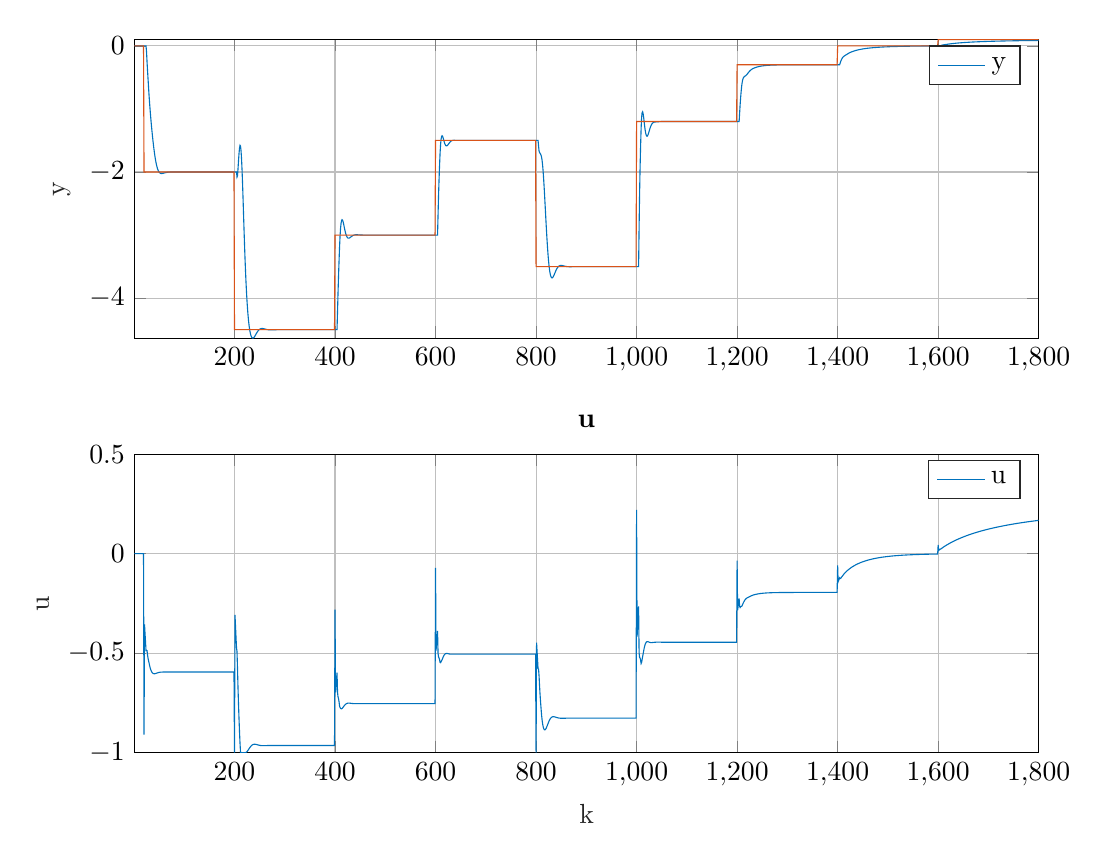
\begin{tikzpicture}

\begin{axis}[%
width=4.521in,
height=1.493in,
at={(0.758in,2.554in)},
scale only axis,
xmin=1,
xmax=1800,
ymin=-4.6335,
ymax=0.1,
ylabel style={font=\color{white!15!black}},
ylabel={y},
axis background/.style={fill=white},
xmajorgrids,
ymajorgrids,
legend style={legend cell align=left, align=left, draw=white!15!black}
]
\addplot [color=mycolor1]
  table[row sep=crcr]{%
1	0\\
2	0\\
3	0\\
4	0\\
5	0\\
6	0\\
7	0\\
8	0\\
9	0\\
10	0\\
11	0\\
12	0\\
13	0\\
14	0\\
15	0\\
16	0\\
17	0\\
18	0\\
19	0\\
20	0\\
21	0\\
22	0\\
23	0\\
24	0\\
25	-0.098378\\
26	-0.25368\\
27	-0.39312\\
28	-0.52557\\
29	-0.65731\\
30	-0.78382\\
31	-0.89914\\
32	-1.0051\\
33	-1.1044\\
34	-1.1976\\
35	-1.2852\\
36	-1.3679\\
37	-1.4461\\
38	-1.5199\\
39	-1.589\\
40	-1.6533\\
41	-1.7125\\
42	-1.7662\\
43	-1.8144\\
44	-1.8568\\
45	-1.8936\\
46	-1.9249\\
47	-1.951\\
48	-1.9721\\
49	-1.9889\\
50	-2.0016\\
51	-2.011\\
52	-2.0174\\
53	-2.0215\\
54	-2.0236\\
55	-2.0242\\
56	-2.0237\\
57	-2.0225\\
58	-2.0207\\
59	-2.0186\\
60	-2.0164\\
61	-2.0142\\
62	-2.0121\\
63	-2.0102\\
64	-2.0085\\
65	-2.0069\\
66	-2.0056\\
67	-2.0044\\
68	-2.0034\\
69	-2.0026\\
70	-2.002\\
71	-2.0014\\
72	-2.001\\
73	-2.0006\\
74	-2.0004\\
75	-2.0002\\
76	-2\\
77	-1.9999\\
78	-1.9998\\
79	-1.9998\\
80	-1.9997\\
81	-1.9997\\
82	-1.9997\\
83	-1.9997\\
84	-1.9997\\
85	-1.9997\\
86	-1.9998\\
87	-1.9998\\
88	-1.9998\\
89	-1.9998\\
90	-1.9999\\
91	-1.9999\\
92	-1.9999\\
93	-1.9999\\
94	-1.9999\\
95	-1.9999\\
96	-2\\
97	-2\\
98	-2\\
99	-2\\
100	-2\\
101	-2\\
102	-2\\
103	-2\\
104	-2\\
105	-2\\
106	-2\\
107	-2\\
108	-2\\
109	-2\\
110	-2\\
111	-2\\
112	-2\\
113	-2\\
114	-2\\
115	-2\\
116	-2\\
117	-2\\
118	-2\\
119	-2\\
120	-2\\
121	-2\\
122	-2\\
123	-2\\
124	-2\\
125	-2\\
126	-2\\
127	-2\\
128	-2\\
129	-2\\
130	-2\\
131	-2\\
132	-2\\
133	-2\\
134	-2\\
135	-2\\
136	-2\\
137	-2\\
138	-2\\
139	-2\\
140	-2\\
141	-2\\
142	-2\\
143	-2\\
144	-2\\
145	-2\\
146	-2\\
147	-2\\
148	-2\\
149	-2\\
150	-2\\
151	-2\\
152	-2\\
153	-2\\
154	-2\\
155	-2\\
156	-2\\
157	-2\\
158	-2\\
159	-2\\
160	-2\\
161	-2\\
162	-2\\
163	-2\\
164	-2\\
165	-2\\
166	-2\\
167	-2\\
168	-2\\
169	-2\\
170	-2\\
171	-2\\
172	-2\\
173	-2\\
174	-2\\
175	-2\\
176	-2\\
177	-2\\
178	-2\\
179	-2\\
180	-2\\
181	-2\\
182	-2\\
183	-2\\
184	-2\\
185	-2\\
186	-2\\
187	-2\\
188	-2\\
189	-2\\
190	-2\\
191	-2\\
192	-2\\
193	-2\\
194	-2\\
195	-2\\
196	-2\\
197	-2\\
198	-2\\
199	-2\\
200	-2\\
201	-2\\
202	-2\\
203	-2\\
204	-2\\
205	-2.0801\\
206	-2.0594\\
207	-1.9505\\
208	-1.8212\\
209	-1.7083\\
210	-1.6218\\
211	-1.578\\
212	-1.5904\\
213	-1.6617\\
214	-1.7873\\
215	-1.9604\\
216	-2.1727\\
217	-2.4144\\
218	-2.6692\\
219	-2.9216\\
220	-3.1617\\
221	-3.3836\\
222	-3.5845\\
223	-3.7634\\
224	-3.9207\\
225	-4.0574\\
226	-4.1752\\
227	-4.2758\\
228	-4.3608\\
229	-4.4317\\
230	-4.4898\\
231	-4.5363\\
232	-4.5724\\
233	-4.5992\\
234	-4.6177\\
235	-4.6288\\
236	-4.6335\\
237	-4.6329\\
238	-4.6279\\
239	-4.6195\\
240	-4.6084\\
241	-4.5957\\
242	-4.5819\\
243	-4.5677\\
244	-4.5538\\
245	-4.5405\\
246	-4.5283\\
247	-4.5174\\
248	-4.5078\\
249	-4.4999\\
250	-4.4934\\
251	-4.4884\\
252	-4.4849\\
253	-4.4826\\
254	-4.4814\\
255	-4.4811\\
256	-4.4817\\
257	-4.4828\\
258	-4.4844\\
259	-4.4863\\
260	-4.4883\\
261	-4.4904\\
262	-4.4925\\
263	-4.4944\\
264	-4.4962\\
265	-4.4978\\
266	-4.4992\\
267	-4.5003\\
268	-4.5012\\
269	-4.5019\\
270	-4.5024\\
271	-4.5027\\
272	-4.5028\\
273	-4.5028\\
274	-4.5027\\
275	-4.5025\\
276	-4.5022\\
277	-4.5019\\
278	-4.5016\\
279	-4.5013\\
280	-4.501\\
281	-4.5007\\
282	-4.5005\\
283	-4.5002\\
284	-4.5\\
285	-4.4999\\
286	-4.4998\\
287	-4.4997\\
288	-4.4996\\
289	-4.4996\\
290	-4.4996\\
291	-4.4996\\
292	-4.4996\\
293	-4.4996\\
294	-4.4997\\
295	-4.4997\\
296	-4.4998\\
297	-4.4998\\
298	-4.4999\\
299	-4.4999\\
300	-4.4999\\
301	-4.5\\
302	-4.5\\
303	-4.5\\
304	-4.5\\
305	-4.5001\\
306	-4.5001\\
307	-4.5001\\
308	-4.5001\\
309	-4.5001\\
310	-4.5001\\
311	-4.5001\\
312	-4.5\\
313	-4.5\\
314	-4.5\\
315	-4.5\\
316	-4.5\\
317	-4.5\\
318	-4.5\\
319	-4.5\\
320	-4.5\\
321	-4.5\\
322	-4.5\\
323	-4.5\\
324	-4.5\\
325	-4.5\\
326	-4.5\\
327	-4.5\\
328	-4.5\\
329	-4.5\\
330	-4.5\\
331	-4.5\\
332	-4.5\\
333	-4.5\\
334	-4.5\\
335	-4.5\\
336	-4.5\\
337	-4.5\\
338	-4.5\\
339	-4.5\\
340	-4.5\\
341	-4.5\\
342	-4.5\\
343	-4.5\\
344	-4.5\\
345	-4.5\\
346	-4.5\\
347	-4.5\\
348	-4.5\\
349	-4.5\\
350	-4.5\\
351	-4.5\\
352	-4.5\\
353	-4.5\\
354	-4.5\\
355	-4.5\\
356	-4.5\\
357	-4.5\\
358	-4.5\\
359	-4.5\\
360	-4.5\\
361	-4.5\\
362	-4.5\\
363	-4.5\\
364	-4.5\\
365	-4.5\\
366	-4.5\\
367	-4.5\\
368	-4.5\\
369	-4.5\\
370	-4.5\\
371	-4.5\\
372	-4.5\\
373	-4.5\\
374	-4.5\\
375	-4.5\\
376	-4.5\\
377	-4.5\\
378	-4.5\\
379	-4.5\\
380	-4.5\\
381	-4.5\\
382	-4.5\\
383	-4.5\\
384	-4.5\\
385	-4.5\\
386	-4.5\\
387	-4.5\\
388	-4.5\\
389	-4.5\\
390	-4.5\\
391	-4.5\\
392	-4.5\\
393	-4.5\\
394	-4.5\\
395	-4.5\\
396	-4.5\\
397	-4.5\\
398	-4.5\\
399	-4.5\\
400	-4.5\\
401	-4.5\\
402	-4.5\\
403	-4.5\\
404	-4.5\\
405	-4.2111\\
406	-3.9122\\
407	-3.6513\\
408	-3.4154\\
409	-3.1953\\
410	-3.0205\\
411	-2.8973\\
412	-2.8167\\
413	-2.7711\\
414	-2.7555\\
415	-2.7635\\
416	-2.7875\\
417	-2.8211\\
418	-2.8594\\
419	-2.8985\\
420	-2.9354\\
421	-2.968\\
422	-2.9952\\
423	-3.0166\\
424	-3.0322\\
425	-3.0424\\
426	-3.0479\\
427	-3.0495\\
428	-3.0481\\
429	-3.0444\\
430	-3.0392\\
431	-3.0333\\
432	-3.0271\\
433	-3.021\\
434	-3.0153\\
435	-3.0103\\
436	-3.006\\
437	-3.0025\\
438	-2.9998\\
439	-2.9977\\
440	-2.9964\\
441	-2.9955\\
442	-2.9951\\
443	-2.9951\\
444	-2.9953\\
445	-2.9957\\
446	-2.9962\\
447	-2.9967\\
448	-2.9973\\
449	-2.9978\\
450	-2.9983\\
451	-2.9988\\
452	-2.9992\\
453	-2.9995\\
454	-2.9997\\
455	-2.9999\\
456	-3.0001\\
457	-3.0002\\
458	-3.0003\\
459	-3.0003\\
460	-3.0003\\
461	-3.0003\\
462	-3.0003\\
463	-3.0003\\
464	-3.0002\\
465	-3.0002\\
466	-3.0002\\
467	-3.0001\\
468	-3.0001\\
469	-3.0001\\
470	-3.0001\\
471	-3\\
472	-3\\
473	-3\\
474	-3\\
475	-3\\
476	-3\\
477	-3\\
478	-3\\
479	-3\\
480	-3\\
481	-3\\
482	-3\\
483	-3\\
484	-3\\
485	-3\\
486	-3\\
487	-3\\
488	-3\\
489	-3\\
490	-3\\
491	-3\\
492	-3\\
493	-3\\
494	-3\\
495	-3\\
496	-3\\
497	-3\\
498	-3\\
499	-3\\
500	-3\\
501	-3\\
502	-3\\
503	-3\\
504	-3\\
505	-3\\
506	-3\\
507	-3\\
508	-3\\
509	-3\\
510	-3\\
511	-3\\
512	-3\\
513	-3\\
514	-3\\
515	-3\\
516	-3\\
517	-3\\
518	-3\\
519	-3\\
520	-3\\
521	-3\\
522	-3\\
523	-3\\
524	-3\\
525	-3\\
526	-3\\
527	-3\\
528	-3\\
529	-3\\
530	-3\\
531	-3\\
532	-3\\
533	-3\\
534	-3\\
535	-3\\
536	-3\\
537	-3\\
538	-3\\
539	-3\\
540	-3\\
541	-3\\
542	-3\\
543	-3\\
544	-3\\
545	-3\\
546	-3\\
547	-3\\
548	-3\\
549	-3\\
550	-3\\
551	-3\\
552	-3\\
553	-3\\
554	-3\\
555	-3\\
556	-3\\
557	-3\\
558	-3\\
559	-3\\
560	-3\\
561	-3\\
562	-3\\
563	-3\\
564	-3\\
565	-3\\
566	-3\\
567	-3\\
568	-3\\
569	-3\\
570	-3\\
571	-3\\
572	-3\\
573	-3\\
574	-3\\
575	-3\\
576	-3\\
577	-3\\
578	-3\\
579	-3\\
580	-3\\
581	-3\\
582	-3\\
583	-3\\
584	-3\\
585	-3\\
586	-3\\
587	-3\\
588	-3\\
589	-3\\
590	-3\\
591	-3\\
592	-3\\
593	-3\\
594	-3\\
595	-3\\
596	-3\\
597	-3\\
598	-3\\
599	-3\\
600	-3\\
601	-3\\
602	-3\\
603	-3\\
604	-3\\
605	-2.6784\\
606	-2.37\\
607	-2.1158\\
608	-1.8985\\
609	-1.706\\
610	-1.5671\\
611	-1.4829\\
612	-1.4393\\
613	-1.4251\\
614	-1.4334\\
615	-1.4562\\
616	-1.4855\\
617	-1.5153\\
618	-1.542\\
619	-1.5631\\
620	-1.5775\\
621	-1.5851\\
622	-1.5865\\
623	-1.5829\\
624	-1.5755\\
625	-1.5658\\
626	-1.5549\\
627	-1.5439\\
628	-1.5334\\
629	-1.5242\\
630	-1.5164\\
631	-1.5101\\
632	-1.5054\\
633	-1.502\\
634	-1.4998\\
635	-1.4985\\
636	-1.4979\\
637	-1.4977\\
638	-1.4979\\
639	-1.4982\\
640	-1.4986\\
641	-1.499\\
642	-1.4993\\
643	-1.4995\\
644	-1.4997\\
645	-1.4997\\
646	-1.4998\\
647	-1.4998\\
648	-1.4997\\
649	-1.4997\\
650	-1.4996\\
651	-1.4996\\
652	-1.4996\\
653	-1.4996\\
654	-1.4996\\
655	-1.4996\\
656	-1.4997\\
657	-1.4997\\
658	-1.4997\\
659	-1.4998\\
660	-1.4998\\
661	-1.4999\\
662	-1.4999\\
663	-1.4999\\
664	-1.4999\\
665	-1.5\\
666	-1.5\\
667	-1.5\\
668	-1.5\\
669	-1.5\\
670	-1.5\\
671	-1.5\\
672	-1.5\\
673	-1.5\\
674	-1.5\\
675	-1.5\\
676	-1.5\\
677	-1.5\\
678	-1.5\\
679	-1.5\\
680	-1.5\\
681	-1.5\\
682	-1.5\\
683	-1.5\\
684	-1.5\\
685	-1.5\\
686	-1.5\\
687	-1.5\\
688	-1.5\\
689	-1.5\\
690	-1.5\\
691	-1.5\\
692	-1.5\\
693	-1.5\\
694	-1.5\\
695	-1.5\\
696	-1.5\\
697	-1.5\\
698	-1.5\\
699	-1.5\\
700	-1.5\\
701	-1.5\\
702	-1.5\\
703	-1.5\\
704	-1.5\\
705	-1.5\\
706	-1.5\\
707	-1.5\\
708	-1.5\\
709	-1.5\\
710	-1.5\\
711	-1.5\\
712	-1.5\\
713	-1.5\\
714	-1.5\\
715	-1.5\\
716	-1.5\\
717	-1.5\\
718	-1.5\\
719	-1.5\\
720	-1.5\\
721	-1.5\\
722	-1.5\\
723	-1.5\\
724	-1.5\\
725	-1.5\\
726	-1.5\\
727	-1.5\\
728	-1.5\\
729	-1.5\\
730	-1.5\\
731	-1.5\\
732	-1.5\\
733	-1.5\\
734	-1.5\\
735	-1.5\\
736	-1.5\\
737	-1.5\\
738	-1.5\\
739	-1.5\\
740	-1.5\\
741	-1.5\\
742	-1.5\\
743	-1.5\\
744	-1.5\\
745	-1.5\\
746	-1.5\\
747	-1.5\\
748	-1.5\\
749	-1.5\\
750	-1.5\\
751	-1.5\\
752	-1.5\\
753	-1.5\\
754	-1.5\\
755	-1.5\\
756	-1.5\\
757	-1.5\\
758	-1.5\\
759	-1.5\\
760	-1.5\\
761	-1.5\\
762	-1.5\\
763	-1.5\\
764	-1.5\\
765	-1.5\\
766	-1.5\\
767	-1.5\\
768	-1.5\\
769	-1.5\\
770	-1.5\\
771	-1.5\\
772	-1.5\\
773	-1.5\\
774	-1.5\\
775	-1.5\\
776	-1.5\\
777	-1.5\\
778	-1.5\\
779	-1.5\\
780	-1.5\\
781	-1.5\\
782	-1.5\\
783	-1.5\\
784	-1.5\\
785	-1.5\\
786	-1.5\\
787	-1.5\\
788	-1.5\\
789	-1.5\\
790	-1.5\\
791	-1.5\\
792	-1.5\\
793	-1.5\\
794	-1.5\\
795	-1.5\\
796	-1.5\\
797	-1.5\\
798	-1.5\\
799	-1.5\\
800	-1.5\\
801	-1.5\\
802	-1.5\\
803	-1.5\\
804	-1.5\\
805	-1.593\\
806	-1.6684\\
807	-1.6941\\
808	-1.7035\\
809	-1.717\\
810	-1.7365\\
811	-1.7668\\
812	-1.8165\\
813	-1.8893\\
814	-1.9843\\
815	-2.0988\\
816	-2.2295\\
817	-2.3721\\
818	-2.5216\\
819	-2.6732\\
820	-2.8226\\
821	-2.9658\\
822	-3.0995\\
823	-3.2213\\
824	-3.3292\\
825	-3.4223\\
826	-3.4999\\
827	-3.5623\\
828	-3.6101\\
829	-3.6442\\
830	-3.666\\
831	-3.6771\\
832	-3.6791\\
833	-3.6737\\
834	-3.6627\\
835	-3.6476\\
836	-3.6298\\
837	-3.6107\\
838	-3.5912\\
839	-3.5723\\
840	-3.5545\\
841	-3.5385\\
842	-3.5244\\
843	-3.5124\\
844	-3.5026\\
845	-3.4949\\
846	-3.4892\\
847	-3.4852\\
848	-3.4827\\
849	-3.4815\\
850	-3.4813\\
851	-3.482\\
852	-3.4833\\
853	-3.4849\\
854	-3.4869\\
855	-3.4889\\
856	-3.4909\\
857	-3.4929\\
858	-3.4947\\
859	-3.4963\\
860	-3.4977\\
861	-3.4988\\
862	-3.4998\\
863	-3.5005\\
864	-3.5011\\
865	-3.5014\\
866	-3.5017\\
867	-3.5018\\
868	-3.5018\\
869	-3.5017\\
870	-3.5016\\
871	-3.5014\\
872	-3.5012\\
873	-3.5011\\
874	-3.5009\\
875	-3.5007\\
876	-3.5005\\
877	-3.5004\\
878	-3.5002\\
879	-3.5001\\
880	-3.5\\
881	-3.5\\
882	-3.4999\\
883	-3.4999\\
884	-3.4998\\
885	-3.4998\\
886	-3.4998\\
887	-3.4998\\
888	-3.4999\\
889	-3.4999\\
890	-3.4999\\
891	-3.4999\\
892	-3.4999\\
893	-3.4999\\
894	-3.5\\
895	-3.5\\
896	-3.5\\
897	-3.5\\
898	-3.5\\
899	-3.5\\
900	-3.5\\
901	-3.5\\
902	-3.5\\
903	-3.5\\
904	-3.5\\
905	-3.5\\
906	-3.5\\
907	-3.5\\
908	-3.5\\
909	-3.5\\
910	-3.5\\
911	-3.5\\
912	-3.5\\
913	-3.5\\
914	-3.5\\
915	-3.5\\
916	-3.5\\
917	-3.5\\
918	-3.5\\
919	-3.5\\
920	-3.5\\
921	-3.5\\
922	-3.5\\
923	-3.5\\
924	-3.5\\
925	-3.5\\
926	-3.5\\
927	-3.5\\
928	-3.5\\
929	-3.5\\
930	-3.5\\
931	-3.5\\
932	-3.5\\
933	-3.5\\
934	-3.5\\
935	-3.5\\
936	-3.5\\
937	-3.5\\
938	-3.5\\
939	-3.5\\
940	-3.5\\
941	-3.5\\
942	-3.5\\
943	-3.5\\
944	-3.5\\
945	-3.5\\
946	-3.5\\
947	-3.5\\
948	-3.5\\
949	-3.5\\
950	-3.5\\
951	-3.5\\
952	-3.5\\
953	-3.5\\
954	-3.5\\
955	-3.5\\
956	-3.5\\
957	-3.5\\
958	-3.5\\
959	-3.5\\
960	-3.5\\
961	-3.5\\
962	-3.5\\
963	-3.5\\
964	-3.5\\
965	-3.5\\
966	-3.5\\
967	-3.5\\
968	-3.5\\
969	-3.5\\
970	-3.5\\
971	-3.5\\
972	-3.5\\
973	-3.5\\
974	-3.5\\
975	-3.5\\
976	-3.5\\
977	-3.5\\
978	-3.5\\
979	-3.5\\
980	-3.5\\
981	-3.5\\
982	-3.5\\
983	-3.5\\
984	-3.5\\
985	-3.5\\
986	-3.5\\
987	-3.5\\
988	-3.5\\
989	-3.5\\
990	-3.5\\
991	-3.5\\
992	-3.5\\
993	-3.5\\
994	-3.5\\
995	-3.5\\
996	-3.5\\
997	-3.5\\
998	-3.5\\
999	-3.5\\
1000	-3.5\\
1001	-3.5\\
1002	-3.5\\
1003	-3.5\\
1004	-3.5\\
1005	-2.8781\\
1006	-2.3361\\
1007	-1.9185\\
1008	-1.5862\\
1009	-1.312\\
1010	-1.138\\
1011	-1.0595\\
1012	-1.0456\\
1013	-1.0737\\
1014	-1.1298\\
1015	-1.1999\\
1016	-1.2704\\
1017	-1.3323\\
1018	-1.3808\\
1019	-1.4136\\
1020	-1.4304\\
1021	-1.4326\\
1022	-1.4228\\
1023	-1.4044\\
1024	-1.3804\\
1025	-1.3538\\
1026	-1.3269\\
1027	-1.3017\\
1028	-1.2792\\
1029	-1.2602\\
1030	-1.2448\\
1031	-1.2328\\
1032	-1.2239\\
1033	-1.2176\\
1034	-1.2133\\
1035	-1.2105\\
1036	-1.2087\\
1037	-1.2076\\
1038	-1.2069\\
1039	-1.2063\\
1040	-1.2057\\
1041	-1.2051\\
1042	-1.2045\\
1043	-1.2038\\
1044	-1.2031\\
1045	-1.2024\\
1046	-1.2018\\
1047	-1.2012\\
1048	-1.2007\\
1049	-1.2003\\
1050	-1.2\\
1051	-1.1998\\
1052	-1.1997\\
1053	-1.1996\\
1054	-1.1995\\
1055	-1.1995\\
1056	-1.1995\\
1057	-1.1996\\
1058	-1.1996\\
1059	-1.1997\\
1060	-1.1997\\
1061	-1.1998\\
1062	-1.1998\\
1063	-1.1998\\
1064	-1.1999\\
1065	-1.1999\\
1066	-1.1999\\
1067	-1.1999\\
1068	-1.1999\\
1069	-1.1999\\
1070	-1.1999\\
1071	-1.1999\\
1072	-1.1999\\
1073	-1.2\\
1074	-1.2\\
1075	-1.2\\
1076	-1.2\\
1077	-1.2\\
1078	-1.2\\
1079	-1.2\\
1080	-1.2\\
1081	-1.2\\
1082	-1.2\\
1083	-1.2\\
1084	-1.2\\
1085	-1.2\\
1086	-1.2\\
1087	-1.2\\
1088	-1.2\\
1089	-1.2\\
1090	-1.2\\
1091	-1.2\\
1092	-1.2\\
1093	-1.2\\
1094	-1.2\\
1095	-1.2\\
1096	-1.2\\
1097	-1.2\\
1098	-1.2\\
1099	-1.2\\
1100	-1.2\\
1101	-1.2\\
1102	-1.2\\
1103	-1.2\\
1104	-1.2\\
1105	-1.2\\
1106	-1.2\\
1107	-1.2\\
1108	-1.2\\
1109	-1.2\\
1110	-1.2\\
1111	-1.2\\
1112	-1.2\\
1113	-1.2\\
1114	-1.2\\
1115	-1.2\\
1116	-1.2\\
1117	-1.2\\
1118	-1.2\\
1119	-1.2\\
1120	-1.2\\
1121	-1.2\\
1122	-1.2\\
1123	-1.2\\
1124	-1.2\\
1125	-1.2\\
1126	-1.2\\
1127	-1.2\\
1128	-1.2\\
1129	-1.2\\
1130	-1.2\\
1131	-1.2\\
1132	-1.2\\
1133	-1.2\\
1134	-1.2\\
1135	-1.2\\
1136	-1.2\\
1137	-1.2\\
1138	-1.2\\
1139	-1.2\\
1140	-1.2\\
1141	-1.2\\
1142	-1.2\\
1143	-1.2\\
1144	-1.2\\
1145	-1.2\\
1146	-1.2\\
1147	-1.2\\
1148	-1.2\\
1149	-1.2\\
1150	-1.2\\
1151	-1.2\\
1152	-1.2\\
1153	-1.2\\
1154	-1.2\\
1155	-1.2\\
1156	-1.2\\
1157	-1.2\\
1158	-1.2\\
1159	-1.2\\
1160	-1.2\\
1161	-1.2\\
1162	-1.2\\
1163	-1.2\\
1164	-1.2\\
1165	-1.2\\
1166	-1.2\\
1167	-1.2\\
1168	-1.2\\
1169	-1.2\\
1170	-1.2\\
1171	-1.2\\
1172	-1.2\\
1173	-1.2\\
1174	-1.2\\
1175	-1.2\\
1176	-1.2\\
1177	-1.2\\
1178	-1.2\\
1179	-1.2\\
1180	-1.2\\
1181	-1.2\\
1182	-1.2\\
1183	-1.2\\
1184	-1.2\\
1185	-1.2\\
1186	-1.2\\
1187	-1.2\\
1188	-1.2\\
1189	-1.2\\
1190	-1.2\\
1191	-1.2\\
1192	-1.2\\
1193	-1.2\\
1194	-1.2\\
1195	-1.2\\
1196	-1.2\\
1197	-1.2\\
1198	-1.2\\
1199	-1.2\\
1200	-1.2\\
1201	-1.2\\
1202	-1.2\\
1203	-1.2\\
1204	-1.2\\
1205	-1.0699\\
1206	-0.9347\\
1207	-0.82309\\
1208	-0.72852\\
1209	-0.64625\\
1210	-0.58455\\
1211	-0.5436\\
1212	-0.51734\\
1213	-0.5008\\
1214	-0.49082\\
1215	-0.4845\\
1216	-0.47924\\
1217	-0.47348\\
1218	-0.46657\\
1219	-0.45837\\
1220	-0.44907\\
1221	-0.43906\\
1222	-0.4288\\
1223	-0.41874\\
1224	-0.40918\\
1225	-0.40036\\
1226	-0.39236\\
1227	-0.38522\\
1228	-0.37887\\
1229	-0.37324\\
1230	-0.36821\\
1231	-0.36369\\
1232	-0.35958\\
1233	-0.3558\\
1234	-0.3523\\
1235	-0.34904\\
1236	-0.34597\\
1237	-0.3431\\
1238	-0.3404\\
1239	-0.33786\\
1240	-0.33549\\
1241	-0.33326\\
1242	-0.33118\\
1243	-0.32924\\
1244	-0.32743\\
1245	-0.32574\\
1246	-0.32417\\
1247	-0.3227\\
1248	-0.32132\\
1249	-0.32003\\
1250	-0.31883\\
1251	-0.3177\\
1252	-0.31664\\
1253	-0.31564\\
1254	-0.31471\\
1255	-0.31383\\
1256	-0.31301\\
1257	-0.31224\\
1258	-0.31151\\
1259	-0.31083\\
1260	-0.31019\\
1261	-0.30959\\
1262	-0.30903\\
1263	-0.30849\\
1264	-0.308\\
1265	-0.30753\\
1266	-0.30709\\
1267	-0.30667\\
1268	-0.30628\\
1269	-0.30591\\
1270	-0.30557\\
1271	-0.30524\\
1272	-0.30494\\
1273	-0.30465\\
1274	-0.30438\\
1275	-0.30412\\
1276	-0.30388\\
1277	-0.30366\\
1278	-0.30344\\
1279	-0.30324\\
1280	-0.30306\\
1281	-0.30288\\
1282	-0.30271\\
1283	-0.30255\\
1284	-0.30241\\
1285	-0.30227\\
1286	-0.30214\\
1287	-0.30201\\
1288	-0.30189\\
1289	-0.30179\\
1290	-0.30168\\
1291	-0.30158\\
1292	-0.30149\\
1293	-0.30141\\
1294	-0.30132\\
1295	-0.30125\\
1296	-0.30118\\
1297	-0.30111\\
1298	-0.30104\\
1299	-0.30098\\
1300	-0.30093\\
1301	-0.30087\\
1302	-0.30082\\
1303	-0.30078\\
1304	-0.30073\\
1305	-0.30069\\
1306	-0.30065\\
1307	-0.30061\\
1308	-0.30058\\
1309	-0.30054\\
1310	-0.30051\\
1311	-0.30048\\
1312	-0.30045\\
1313	-0.30043\\
1314	-0.3004\\
1315	-0.30038\\
1316	-0.30036\\
1317	-0.30034\\
1318	-0.30032\\
1319	-0.3003\\
1320	-0.30028\\
1321	-0.30027\\
1322	-0.30025\\
1323	-0.30024\\
1324	-0.30022\\
1325	-0.30021\\
1326	-0.3002\\
1327	-0.30019\\
1328	-0.30018\\
1329	-0.30017\\
1330	-0.30016\\
1331	-0.30015\\
1332	-0.30014\\
1333	-0.30013\\
1334	-0.30012\\
1335	-0.30012\\
1336	-0.30011\\
1337	-0.3001\\
1338	-0.3001\\
1339	-0.30009\\
1340	-0.30009\\
1341	-0.30008\\
1342	-0.30008\\
1343	-0.30007\\
1344	-0.30007\\
1345	-0.30006\\
1346	-0.30006\\
1347	-0.30006\\
1348	-0.30005\\
1349	-0.30005\\
1350	-0.30005\\
1351	-0.30004\\
1352	-0.30004\\
1353	-0.30004\\
1354	-0.30004\\
1355	-0.30004\\
1356	-0.30003\\
1357	-0.30003\\
1358	-0.30003\\
1359	-0.30003\\
1360	-0.30003\\
1361	-0.30002\\
1362	-0.30002\\
1363	-0.30002\\
1364	-0.30002\\
1365	-0.30002\\
1366	-0.30002\\
1367	-0.30002\\
1368	-0.30002\\
1369	-0.30002\\
1370	-0.30001\\
1371	-0.30001\\
1372	-0.30001\\
1373	-0.30001\\
1374	-0.30001\\
1375	-0.30001\\
1376	-0.30001\\
1377	-0.30001\\
1378	-0.30001\\
1379	-0.30001\\
1380	-0.30001\\
1381	-0.30001\\
1382	-0.30001\\
1383	-0.30001\\
1384	-0.30001\\
1385	-0.30001\\
1386	-0.30001\\
1387	-0.30001\\
1388	-0.3\\
1389	-0.3\\
1390	-0.3\\
1391	-0.3\\
1392	-0.3\\
1393	-0.3\\
1394	-0.3\\
1395	-0.3\\
1396	-0.3\\
1397	-0.3\\
1398	-0.3\\
1399	-0.3\\
1400	-0.3\\
1401	-0.3\\
1402	-0.3\\
1403	-0.3\\
1404	-0.3\\
1405	-0.2777\\
1406	-0.25099\\
1407	-0.22962\\
1408	-0.21197\\
1409	-0.19682\\
1410	-0.18468\\
1411	-0.17556\\
1412	-0.16843\\
1413	-0.16241\\
1414	-0.15703\\
1415	-0.15197\\
1416	-0.14699\\
1417	-0.14201\\
1418	-0.13702\\
1419	-0.13207\\
1420	-0.12722\\
1421	-0.12252\\
1422	-0.11802\\
1423	-0.11374\\
1424	-0.10968\\
1425	-0.10584\\
1426	-0.10221\\
1427	-0.098772\\
1428	-0.095507\\
1429	-0.092401\\
1430	-0.089439\\
1431	-0.086609\\
1432	-0.0839\\
1433	-0.081305\\
1434	-0.078818\\
1435	-0.076431\\
1436	-0.07414\\
1437	-0.07194\\
1438	-0.069826\\
1439	-0.067794\\
1440	-0.06584\\
1441	-0.063961\\
1442	-0.062151\\
1443	-0.060408\\
1444	-0.058729\\
1445	-0.05711\\
1446	-0.055548\\
1447	-0.054041\\
1448	-0.052586\\
1449	-0.051181\\
1450	-0.049823\\
1451	-0.04851\\
1452	-0.047241\\
1453	-0.046014\\
1454	-0.044826\\
1455	-0.043676\\
1456	-0.042563\\
1457	-0.041484\\
1458	-0.040439\\
1459	-0.039427\\
1460	-0.038445\\
1461	-0.037493\\
1462	-0.03657\\
1463	-0.035674\\
1464	-0.034804\\
1465	-0.03396\\
1466	-0.03314\\
1467	-0.032344\\
1468	-0.031571\\
1469	-0.030819\\
1470	-0.030089\\
1471	-0.029379\\
1472	-0.028689\\
1473	-0.028018\\
1474	-0.027365\\
1475	-0.02673\\
1476	-0.026112\\
1477	-0.02551\\
1478	-0.024925\\
1479	-0.024355\\
1480	-0.0238\\
1481	-0.02326\\
1482	-0.022733\\
1483	-0.02222\\
1484	-0.021721\\
1485	-0.021234\\
1486	-0.02076\\
1487	-0.020297\\
1488	-0.019846\\
1489	-0.019407\\
1490	-0.018978\\
1491	-0.01856\\
1492	-0.018153\\
1493	-0.017755\\
1494	-0.017367\\
1495	-0.016988\\
1496	-0.016619\\
1497	-0.016259\\
1498	-0.015907\\
1499	-0.015564\\
1500	-0.015228\\
1501	-0.014901\\
1502	-0.014582\\
1503	-0.01427\\
1504	-0.013965\\
1505	-0.013667\\
1506	-0.013377\\
1507	-0.013093\\
1508	-0.012815\\
1509	-0.012544\\
1510	-0.01228\\
1511	-0.012021\\
1512	-0.011768\\
1513	-0.011521\\
1514	-0.01128\\
1515	-0.011044\\
1516	-0.010813\\
1517	-0.010587\\
1518	-0.010367\\
1519	-0.010151\\
1520	-0.0099404\\
1521	-0.0097343\\
1522	-0.0095328\\
1523	-0.0093357\\
1524	-0.009143\\
1525	-0.0089545\\
1526	-0.0087701\\
1527	-0.0085897\\
1528	-0.0084133\\
1529	-0.0082407\\
1530	-0.0080719\\
1531	-0.0079067\\
1532	-0.0077451\\
1533	-0.0075869\\
1534	-0.0074322\\
1535	-0.0072808\\
1536	-0.0071326\\
1537	-0.0069876\\
1538	-0.0068457\\
1539	-0.0067068\\
1540	-0.0065709\\
1541	-0.0064378\\
1542	-0.0063076\\
1543	-0.0061801\\
1544	-0.0060553\\
1545	-0.0059332\\
1546	-0.0058136\\
1547	-0.0056965\\
1548	-0.0055819\\
1549	-0.0054696\\
1550	-0.0053597\\
1551	-0.0052521\\
1552	-0.0051468\\
1553	-0.0050436\\
1554	-0.0049426\\
1555	-0.0048437\\
1556	-0.0047468\\
1557	-0.004652\\
1558	-0.0045591\\
1559	-0.0044681\\
1560	-0.0043789\\
1561	-0.0042917\\
1562	-0.0042062\\
1563	-0.0041224\\
1564	-0.0040404\\
1565	-0.0039601\\
1566	-0.0038814\\
1567	-0.0038043\\
1568	-0.0037288\\
1569	-0.0036548\\
1570	-0.0035823\\
1571	-0.0035114\\
1572	-0.0034418\\
1573	-0.0033737\\
1574	-0.0033069\\
1575	-0.0032415\\
1576	-0.0031774\\
1577	-0.0031146\\
1578	-0.0030531\\
1579	-0.0029929\\
1580	-0.0029338\\
1581	-0.0028759\\
1582	-0.0028192\\
1583	-0.0027637\\
1584	-0.0027092\\
1585	-0.0026559\\
1586	-0.0026036\\
1587	-0.0025524\\
1588	-0.0025022\\
1589	-0.002453\\
1590	-0.0024048\\
1591	-0.0023575\\
1592	-0.0023112\\
1593	-0.0022659\\
1594	-0.0022214\\
1595	-0.0021778\\
1596	-0.0021351\\
1597	-0.0020932\\
1598	-0.0020522\\
1599	-0.002012\\
1600	-0.0019726\\
1601	-0.0019339\\
1602	-0.0018961\\
1603	-0.001859\\
1604	-0.0018226\\
1605	0.0010104\\
1606	0.0054261\\
1607	0.0085557\\
1608	0.010921\\
1609	0.012857\\
1610	0.014497\\
1611	0.015877\\
1612	0.017104\\
1613	0.018289\\
1614	0.019473\\
1615	0.020666\\
1616	0.021868\\
1617	0.02307\\
1618	0.024265\\
1619	0.025443\\
1620	0.026598\\
1621	0.027724\\
1622	0.028822\\
1623	0.02989\\
1624	0.03093\\
1625	0.031942\\
1626	0.032928\\
1627	0.033889\\
1628	0.034826\\
1629	0.035741\\
1630	0.036634\\
1631	0.037506\\
1632	0.038358\\
1633	0.03919\\
1634	0.040004\\
1635	0.040799\\
1636	0.041576\\
1637	0.042336\\
1638	0.043079\\
1639	0.043806\\
1640	0.044518\\
1641	0.045214\\
1642	0.045896\\
1643	0.046563\\
1644	0.047217\\
1645	0.047858\\
1646	0.048485\\
1647	0.0491\\
1648	0.049703\\
1649	0.050293\\
1650	0.050873\\
1651	0.051441\\
1652	0.051998\\
1653	0.052544\\
1654	0.05308\\
1655	0.053607\\
1656	0.054123\\
1657	0.05463\\
1658	0.055128\\
1659	0.055617\\
1660	0.056097\\
1661	0.056569\\
1662	0.057032\\
1663	0.057487\\
1664	0.057934\\
1665	0.058374\\
1666	0.058806\\
1667	0.059231\\
1668	0.059649\\
1669	0.060059\\
1670	0.060463\\
1671	0.060861\\
1672	0.061251\\
1673	0.061636\\
1674	0.062014\\
1675	0.062387\\
1676	0.062753\\
1677	0.063114\\
1678	0.063469\\
1679	0.063819\\
1680	0.064163\\
1681	0.064502\\
1682	0.064836\\
1683	0.065165\\
1684	0.065489\\
1685	0.065808\\
1686	0.066122\\
1687	0.066432\\
1688	0.066738\\
1689	0.067039\\
1690	0.067335\\
1691	0.067628\\
1692	0.067916\\
1693	0.0682\\
1694	0.068481\\
1695	0.068757\\
1696	0.069029\\
1697	0.069298\\
1698	0.069563\\
1699	0.069825\\
1700	0.070083\\
1701	0.070338\\
1702	0.070589\\
1703	0.070837\\
1704	0.071082\\
1705	0.071323\\
1706	0.071561\\
1707	0.071797\\
1708	0.072029\\
1709	0.072258\\
1710	0.072484\\
1711	0.072708\\
1712	0.072929\\
1713	0.073147\\
1714	0.073362\\
1715	0.073575\\
1716	0.073785\\
1717	0.073992\\
1718	0.074197\\
1719	0.074399\\
1720	0.074599\\
1721	0.074797\\
1722	0.074992\\
1723	0.075185\\
1724	0.075376\\
1725	0.075565\\
1726	0.075751\\
1727	0.075935\\
1728	0.076117\\
1729	0.076297\\
1730	0.076475\\
1731	0.076651\\
1732	0.076825\\
1733	0.076997\\
1734	0.077167\\
1735	0.077335\\
1736	0.077501\\
1737	0.077666\\
1738	0.077828\\
1739	0.077989\\
1740	0.078149\\
1741	0.078306\\
1742	0.078462\\
1743	0.078616\\
1744	0.078768\\
1745	0.078919\\
1746	0.079068\\
1747	0.079216\\
1748	0.079362\\
1749	0.079507\\
1750	0.07965\\
1751	0.079792\\
1752	0.079932\\
1753	0.080071\\
1754	0.080208\\
1755	0.080344\\
1756	0.080479\\
1757	0.080612\\
1758	0.080744\\
1759	0.080874\\
1760	0.081004\\
1761	0.081132\\
1762	0.081259\\
1763	0.081384\\
1764	0.081508\\
1765	0.081632\\
1766	0.081753\\
1767	0.081874\\
1768	0.081994\\
1769	0.082112\\
1770	0.08223\\
1771	0.082346\\
1772	0.082461\\
1773	0.082575\\
1774	0.082688\\
1775	0.0828\\
1776	0.082911\\
1777	0.083021\\
1778	0.08313\\
1779	0.083238\\
1780	0.083344\\
1781	0.08345\\
1782	0.083555\\
1783	0.083659\\
1784	0.083762\\
1785	0.083865\\
1786	0.083966\\
1787	0.084066\\
1788	0.084166\\
1789	0.084264\\
1790	0.084362\\
1791	0.084459\\
1792	0.084555\\
1793	0.08465\\
1794	0.084744\\
1795	0.084838\\
1796	0.08493\\
1797	0.085022\\
1798	0.085114\\
1799	0.085204\\
1800	0.085294\\
};
\addlegendentry{y}

\addplot [color=mycolor2, forget plot]
  table[row sep=crcr]{%
1	0\\
2	0\\
3	0\\
4	0\\
5	0\\
6	0\\
7	0\\
8	0\\
9	0\\
10	0\\
11	0\\
12	0\\
13	0\\
14	0\\
15	0\\
16	0\\
17	0\\
18	0\\
19	0\\
20	-2\\
21	-2\\
22	-2\\
23	-2\\
24	-2\\
25	-2\\
26	-2\\
27	-2\\
28	-2\\
29	-2\\
30	-2\\
31	-2\\
32	-2\\
33	-2\\
34	-2\\
35	-2\\
36	-2\\
37	-2\\
38	-2\\
39	-2\\
40	-2\\
41	-2\\
42	-2\\
43	-2\\
44	-2\\
45	-2\\
46	-2\\
47	-2\\
48	-2\\
49	-2\\
50	-2\\
51	-2\\
52	-2\\
53	-2\\
54	-2\\
55	-2\\
56	-2\\
57	-2\\
58	-2\\
59	-2\\
60	-2\\
61	-2\\
62	-2\\
63	-2\\
64	-2\\
65	-2\\
66	-2\\
67	-2\\
68	-2\\
69	-2\\
70	-2\\
71	-2\\
72	-2\\
73	-2\\
74	-2\\
75	-2\\
76	-2\\
77	-2\\
78	-2\\
79	-2\\
80	-2\\
81	-2\\
82	-2\\
83	-2\\
84	-2\\
85	-2\\
86	-2\\
87	-2\\
88	-2\\
89	-2\\
90	-2\\
91	-2\\
92	-2\\
93	-2\\
94	-2\\
95	-2\\
96	-2\\
97	-2\\
98	-2\\
99	-2\\
100	-2\\
101	-2\\
102	-2\\
103	-2\\
104	-2\\
105	-2\\
106	-2\\
107	-2\\
108	-2\\
109	-2\\
110	-2\\
111	-2\\
112	-2\\
113	-2\\
114	-2\\
115	-2\\
116	-2\\
117	-2\\
118	-2\\
119	-2\\
120	-2\\
121	-2\\
122	-2\\
123	-2\\
124	-2\\
125	-2\\
126	-2\\
127	-2\\
128	-2\\
129	-2\\
130	-2\\
131	-2\\
132	-2\\
133	-2\\
134	-2\\
135	-2\\
136	-2\\
137	-2\\
138	-2\\
139	-2\\
140	-2\\
141	-2\\
142	-2\\
143	-2\\
144	-2\\
145	-2\\
146	-2\\
147	-2\\
148	-2\\
149	-2\\
150	-2\\
151	-2\\
152	-2\\
153	-2\\
154	-2\\
155	-2\\
156	-2\\
157	-2\\
158	-2\\
159	-2\\
160	-2\\
161	-2\\
162	-2\\
163	-2\\
164	-2\\
165	-2\\
166	-2\\
167	-2\\
168	-2\\
169	-2\\
170	-2\\
171	-2\\
172	-2\\
173	-2\\
174	-2\\
175	-2\\
176	-2\\
177	-2\\
178	-2\\
179	-2\\
180	-2\\
181	-2\\
182	-2\\
183	-2\\
184	-2\\
185	-2\\
186	-2\\
187	-2\\
188	-2\\
189	-2\\
190	-2\\
191	-2\\
192	-2\\
193	-2\\
194	-2\\
195	-2\\
196	-2\\
197	-2\\
198	-2\\
199	-2\\
200	-4.5\\
201	-4.5\\
202	-4.5\\
203	-4.5\\
204	-4.5\\
205	-4.5\\
206	-4.5\\
207	-4.5\\
208	-4.5\\
209	-4.5\\
210	-4.5\\
211	-4.5\\
212	-4.5\\
213	-4.5\\
214	-4.5\\
215	-4.5\\
216	-4.5\\
217	-4.5\\
218	-4.5\\
219	-4.5\\
220	-4.5\\
221	-4.5\\
222	-4.5\\
223	-4.5\\
224	-4.5\\
225	-4.5\\
226	-4.5\\
227	-4.5\\
228	-4.5\\
229	-4.5\\
230	-4.5\\
231	-4.5\\
232	-4.5\\
233	-4.5\\
234	-4.5\\
235	-4.5\\
236	-4.5\\
237	-4.5\\
238	-4.5\\
239	-4.5\\
240	-4.5\\
241	-4.5\\
242	-4.5\\
243	-4.5\\
244	-4.5\\
245	-4.5\\
246	-4.5\\
247	-4.5\\
248	-4.5\\
249	-4.5\\
250	-4.5\\
251	-4.5\\
252	-4.5\\
253	-4.5\\
254	-4.5\\
255	-4.5\\
256	-4.5\\
257	-4.5\\
258	-4.5\\
259	-4.5\\
260	-4.5\\
261	-4.5\\
262	-4.5\\
263	-4.5\\
264	-4.5\\
265	-4.5\\
266	-4.5\\
267	-4.5\\
268	-4.5\\
269	-4.5\\
270	-4.5\\
271	-4.5\\
272	-4.5\\
273	-4.5\\
274	-4.5\\
275	-4.5\\
276	-4.5\\
277	-4.5\\
278	-4.5\\
279	-4.5\\
280	-4.5\\
281	-4.5\\
282	-4.5\\
283	-4.5\\
284	-4.5\\
285	-4.5\\
286	-4.5\\
287	-4.5\\
288	-4.5\\
289	-4.5\\
290	-4.5\\
291	-4.5\\
292	-4.5\\
293	-4.5\\
294	-4.5\\
295	-4.5\\
296	-4.5\\
297	-4.5\\
298	-4.5\\
299	-4.5\\
300	-4.5\\
301	-4.5\\
302	-4.5\\
303	-4.5\\
304	-4.5\\
305	-4.5\\
306	-4.5\\
307	-4.5\\
308	-4.5\\
309	-4.5\\
310	-4.5\\
311	-4.5\\
312	-4.5\\
313	-4.5\\
314	-4.5\\
315	-4.5\\
316	-4.5\\
317	-4.5\\
318	-4.5\\
319	-4.5\\
320	-4.5\\
321	-4.5\\
322	-4.5\\
323	-4.5\\
324	-4.5\\
325	-4.5\\
326	-4.5\\
327	-4.5\\
328	-4.5\\
329	-4.5\\
330	-4.5\\
331	-4.5\\
332	-4.5\\
333	-4.5\\
334	-4.5\\
335	-4.5\\
336	-4.5\\
337	-4.5\\
338	-4.5\\
339	-4.5\\
340	-4.5\\
341	-4.5\\
342	-4.5\\
343	-4.5\\
344	-4.5\\
345	-4.5\\
346	-4.5\\
347	-4.5\\
348	-4.5\\
349	-4.5\\
350	-4.5\\
351	-4.5\\
352	-4.5\\
353	-4.5\\
354	-4.5\\
355	-4.5\\
356	-4.5\\
357	-4.5\\
358	-4.5\\
359	-4.5\\
360	-4.5\\
361	-4.5\\
362	-4.5\\
363	-4.5\\
364	-4.5\\
365	-4.5\\
366	-4.5\\
367	-4.5\\
368	-4.5\\
369	-4.5\\
370	-4.5\\
371	-4.5\\
372	-4.5\\
373	-4.5\\
374	-4.5\\
375	-4.5\\
376	-4.5\\
377	-4.5\\
378	-4.5\\
379	-4.5\\
380	-4.5\\
381	-4.5\\
382	-4.5\\
383	-4.5\\
384	-4.5\\
385	-4.5\\
386	-4.5\\
387	-4.5\\
388	-4.5\\
389	-4.5\\
390	-4.5\\
391	-4.5\\
392	-4.5\\
393	-4.5\\
394	-4.5\\
395	-4.5\\
396	-4.5\\
397	-4.5\\
398	-4.5\\
399	-4.5\\
400	-3\\
401	-3\\
402	-3\\
403	-3\\
404	-3\\
405	-3\\
406	-3\\
407	-3\\
408	-3\\
409	-3\\
410	-3\\
411	-3\\
412	-3\\
413	-3\\
414	-3\\
415	-3\\
416	-3\\
417	-3\\
418	-3\\
419	-3\\
420	-3\\
421	-3\\
422	-3\\
423	-3\\
424	-3\\
425	-3\\
426	-3\\
427	-3\\
428	-3\\
429	-3\\
430	-3\\
431	-3\\
432	-3\\
433	-3\\
434	-3\\
435	-3\\
436	-3\\
437	-3\\
438	-3\\
439	-3\\
440	-3\\
441	-3\\
442	-3\\
443	-3\\
444	-3\\
445	-3\\
446	-3\\
447	-3\\
448	-3\\
449	-3\\
450	-3\\
451	-3\\
452	-3\\
453	-3\\
454	-3\\
455	-3\\
456	-3\\
457	-3\\
458	-3\\
459	-3\\
460	-3\\
461	-3\\
462	-3\\
463	-3\\
464	-3\\
465	-3\\
466	-3\\
467	-3\\
468	-3\\
469	-3\\
470	-3\\
471	-3\\
472	-3\\
473	-3\\
474	-3\\
475	-3\\
476	-3\\
477	-3\\
478	-3\\
479	-3\\
480	-3\\
481	-3\\
482	-3\\
483	-3\\
484	-3\\
485	-3\\
486	-3\\
487	-3\\
488	-3\\
489	-3\\
490	-3\\
491	-3\\
492	-3\\
493	-3\\
494	-3\\
495	-3\\
496	-3\\
497	-3\\
498	-3\\
499	-3\\
500	-3\\
501	-3\\
502	-3\\
503	-3\\
504	-3\\
505	-3\\
506	-3\\
507	-3\\
508	-3\\
509	-3\\
510	-3\\
511	-3\\
512	-3\\
513	-3\\
514	-3\\
515	-3\\
516	-3\\
517	-3\\
518	-3\\
519	-3\\
520	-3\\
521	-3\\
522	-3\\
523	-3\\
524	-3\\
525	-3\\
526	-3\\
527	-3\\
528	-3\\
529	-3\\
530	-3\\
531	-3\\
532	-3\\
533	-3\\
534	-3\\
535	-3\\
536	-3\\
537	-3\\
538	-3\\
539	-3\\
540	-3\\
541	-3\\
542	-3\\
543	-3\\
544	-3\\
545	-3\\
546	-3\\
547	-3\\
548	-3\\
549	-3\\
550	-3\\
551	-3\\
552	-3\\
553	-3\\
554	-3\\
555	-3\\
556	-3\\
557	-3\\
558	-3\\
559	-3\\
560	-3\\
561	-3\\
562	-3\\
563	-3\\
564	-3\\
565	-3\\
566	-3\\
567	-3\\
568	-3\\
569	-3\\
570	-3\\
571	-3\\
572	-3\\
573	-3\\
574	-3\\
575	-3\\
576	-3\\
577	-3\\
578	-3\\
579	-3\\
580	-3\\
581	-3\\
582	-3\\
583	-3\\
584	-3\\
585	-3\\
586	-3\\
587	-3\\
588	-3\\
589	-3\\
590	-3\\
591	-3\\
592	-3\\
593	-3\\
594	-3\\
595	-3\\
596	-3\\
597	-3\\
598	-3\\
599	-3\\
600	-1.5\\
601	-1.5\\
602	-1.5\\
603	-1.5\\
604	-1.5\\
605	-1.5\\
606	-1.5\\
607	-1.5\\
608	-1.5\\
609	-1.5\\
610	-1.5\\
611	-1.5\\
612	-1.5\\
613	-1.5\\
614	-1.5\\
615	-1.5\\
616	-1.5\\
617	-1.5\\
618	-1.5\\
619	-1.5\\
620	-1.5\\
621	-1.5\\
622	-1.5\\
623	-1.5\\
624	-1.5\\
625	-1.5\\
626	-1.5\\
627	-1.5\\
628	-1.5\\
629	-1.5\\
630	-1.5\\
631	-1.5\\
632	-1.5\\
633	-1.5\\
634	-1.5\\
635	-1.5\\
636	-1.5\\
637	-1.5\\
638	-1.5\\
639	-1.5\\
640	-1.5\\
641	-1.5\\
642	-1.5\\
643	-1.5\\
644	-1.5\\
645	-1.5\\
646	-1.5\\
647	-1.5\\
648	-1.5\\
649	-1.5\\
650	-1.5\\
651	-1.5\\
652	-1.5\\
653	-1.5\\
654	-1.5\\
655	-1.5\\
656	-1.5\\
657	-1.5\\
658	-1.5\\
659	-1.5\\
660	-1.5\\
661	-1.5\\
662	-1.5\\
663	-1.5\\
664	-1.5\\
665	-1.5\\
666	-1.5\\
667	-1.5\\
668	-1.5\\
669	-1.5\\
670	-1.5\\
671	-1.5\\
672	-1.5\\
673	-1.5\\
674	-1.5\\
675	-1.5\\
676	-1.5\\
677	-1.5\\
678	-1.5\\
679	-1.5\\
680	-1.5\\
681	-1.5\\
682	-1.5\\
683	-1.5\\
684	-1.5\\
685	-1.5\\
686	-1.5\\
687	-1.5\\
688	-1.5\\
689	-1.5\\
690	-1.5\\
691	-1.5\\
692	-1.5\\
693	-1.5\\
694	-1.5\\
695	-1.5\\
696	-1.5\\
697	-1.5\\
698	-1.5\\
699	-1.5\\
700	-1.5\\
701	-1.5\\
702	-1.5\\
703	-1.5\\
704	-1.5\\
705	-1.5\\
706	-1.5\\
707	-1.5\\
708	-1.5\\
709	-1.5\\
710	-1.5\\
711	-1.5\\
712	-1.5\\
713	-1.5\\
714	-1.5\\
715	-1.5\\
716	-1.5\\
717	-1.5\\
718	-1.5\\
719	-1.5\\
720	-1.5\\
721	-1.5\\
722	-1.5\\
723	-1.5\\
724	-1.5\\
725	-1.5\\
726	-1.5\\
727	-1.5\\
728	-1.5\\
729	-1.5\\
730	-1.5\\
731	-1.5\\
732	-1.5\\
733	-1.5\\
734	-1.5\\
735	-1.5\\
736	-1.5\\
737	-1.5\\
738	-1.5\\
739	-1.5\\
740	-1.5\\
741	-1.5\\
742	-1.5\\
743	-1.5\\
744	-1.5\\
745	-1.5\\
746	-1.5\\
747	-1.5\\
748	-1.5\\
749	-1.5\\
750	-1.5\\
751	-1.5\\
752	-1.5\\
753	-1.5\\
754	-1.5\\
755	-1.5\\
756	-1.5\\
757	-1.5\\
758	-1.5\\
759	-1.5\\
760	-1.5\\
761	-1.5\\
762	-1.5\\
763	-1.5\\
764	-1.5\\
765	-1.5\\
766	-1.5\\
767	-1.5\\
768	-1.5\\
769	-1.5\\
770	-1.5\\
771	-1.5\\
772	-1.5\\
773	-1.5\\
774	-1.5\\
775	-1.5\\
776	-1.5\\
777	-1.5\\
778	-1.5\\
779	-1.5\\
780	-1.5\\
781	-1.5\\
782	-1.5\\
783	-1.5\\
784	-1.5\\
785	-1.5\\
786	-1.5\\
787	-1.5\\
788	-1.5\\
789	-1.5\\
790	-1.5\\
791	-1.5\\
792	-1.5\\
793	-1.5\\
794	-1.5\\
795	-1.5\\
796	-1.5\\
797	-1.5\\
798	-1.5\\
799	-1.5\\
800	-3.5\\
801	-3.5\\
802	-3.5\\
803	-3.5\\
804	-3.5\\
805	-3.5\\
806	-3.5\\
807	-3.5\\
808	-3.5\\
809	-3.5\\
810	-3.5\\
811	-3.5\\
812	-3.5\\
813	-3.5\\
814	-3.5\\
815	-3.5\\
816	-3.5\\
817	-3.5\\
818	-3.5\\
819	-3.5\\
820	-3.5\\
821	-3.5\\
822	-3.5\\
823	-3.5\\
824	-3.5\\
825	-3.5\\
826	-3.5\\
827	-3.5\\
828	-3.5\\
829	-3.5\\
830	-3.5\\
831	-3.5\\
832	-3.5\\
833	-3.5\\
834	-3.5\\
835	-3.5\\
836	-3.5\\
837	-3.5\\
838	-3.5\\
839	-3.5\\
840	-3.5\\
841	-3.5\\
842	-3.5\\
843	-3.5\\
844	-3.5\\
845	-3.5\\
846	-3.5\\
847	-3.5\\
848	-3.5\\
849	-3.5\\
850	-3.5\\
851	-3.5\\
852	-3.5\\
853	-3.5\\
854	-3.5\\
855	-3.5\\
856	-3.5\\
857	-3.5\\
858	-3.5\\
859	-3.5\\
860	-3.5\\
861	-3.5\\
862	-3.5\\
863	-3.5\\
864	-3.5\\
865	-3.5\\
866	-3.5\\
867	-3.5\\
868	-3.5\\
869	-3.5\\
870	-3.5\\
871	-3.5\\
872	-3.5\\
873	-3.5\\
874	-3.5\\
875	-3.5\\
876	-3.5\\
877	-3.5\\
878	-3.5\\
879	-3.5\\
880	-3.5\\
881	-3.5\\
882	-3.5\\
883	-3.5\\
884	-3.5\\
885	-3.5\\
886	-3.5\\
887	-3.5\\
888	-3.5\\
889	-3.5\\
890	-3.5\\
891	-3.5\\
892	-3.5\\
893	-3.5\\
894	-3.5\\
895	-3.5\\
896	-3.5\\
897	-3.5\\
898	-3.5\\
899	-3.5\\
900	-3.5\\
901	-3.5\\
902	-3.5\\
903	-3.5\\
904	-3.5\\
905	-3.5\\
906	-3.5\\
907	-3.5\\
908	-3.5\\
909	-3.5\\
910	-3.5\\
911	-3.5\\
912	-3.5\\
913	-3.5\\
914	-3.5\\
915	-3.5\\
916	-3.5\\
917	-3.5\\
918	-3.5\\
919	-3.5\\
920	-3.5\\
921	-3.5\\
922	-3.5\\
923	-3.5\\
924	-3.5\\
925	-3.5\\
926	-3.5\\
927	-3.5\\
928	-3.5\\
929	-3.5\\
930	-3.5\\
931	-3.5\\
932	-3.5\\
933	-3.5\\
934	-3.5\\
935	-3.5\\
936	-3.5\\
937	-3.5\\
938	-3.5\\
939	-3.5\\
940	-3.5\\
941	-3.5\\
942	-3.5\\
943	-3.5\\
944	-3.5\\
945	-3.5\\
946	-3.5\\
947	-3.5\\
948	-3.5\\
949	-3.5\\
950	-3.5\\
951	-3.5\\
952	-3.5\\
953	-3.5\\
954	-3.5\\
955	-3.5\\
956	-3.5\\
957	-3.5\\
958	-3.5\\
959	-3.5\\
960	-3.5\\
961	-3.5\\
962	-3.5\\
963	-3.5\\
964	-3.5\\
965	-3.5\\
966	-3.5\\
967	-3.5\\
968	-3.5\\
969	-3.5\\
970	-3.5\\
971	-3.5\\
972	-3.5\\
973	-3.5\\
974	-3.5\\
975	-3.5\\
976	-3.5\\
977	-3.5\\
978	-3.5\\
979	-3.5\\
980	-3.5\\
981	-3.5\\
982	-3.5\\
983	-3.5\\
984	-3.5\\
985	-3.5\\
986	-3.5\\
987	-3.5\\
988	-3.5\\
989	-3.5\\
990	-3.5\\
991	-3.5\\
992	-3.5\\
993	-3.5\\
994	-3.5\\
995	-3.5\\
996	-3.5\\
997	-3.5\\
998	-3.5\\
999	-3.5\\
1000	-1.2\\
1001	-1.2\\
1002	-1.2\\
1003	-1.2\\
1004	-1.2\\
1005	-1.2\\
1006	-1.2\\
1007	-1.2\\
1008	-1.2\\
1009	-1.2\\
1010	-1.2\\
1011	-1.2\\
1012	-1.2\\
1013	-1.2\\
1014	-1.2\\
1015	-1.2\\
1016	-1.2\\
1017	-1.2\\
1018	-1.2\\
1019	-1.2\\
1020	-1.2\\
1021	-1.2\\
1022	-1.2\\
1023	-1.2\\
1024	-1.2\\
1025	-1.2\\
1026	-1.2\\
1027	-1.2\\
1028	-1.2\\
1029	-1.2\\
1030	-1.2\\
1031	-1.2\\
1032	-1.2\\
1033	-1.2\\
1034	-1.2\\
1035	-1.2\\
1036	-1.2\\
1037	-1.2\\
1038	-1.2\\
1039	-1.2\\
1040	-1.2\\
1041	-1.2\\
1042	-1.2\\
1043	-1.2\\
1044	-1.2\\
1045	-1.2\\
1046	-1.2\\
1047	-1.2\\
1048	-1.2\\
1049	-1.2\\
1050	-1.2\\
1051	-1.2\\
1052	-1.2\\
1053	-1.2\\
1054	-1.2\\
1055	-1.2\\
1056	-1.2\\
1057	-1.2\\
1058	-1.2\\
1059	-1.2\\
1060	-1.2\\
1061	-1.2\\
1062	-1.2\\
1063	-1.2\\
1064	-1.2\\
1065	-1.2\\
1066	-1.2\\
1067	-1.2\\
1068	-1.2\\
1069	-1.2\\
1070	-1.2\\
1071	-1.2\\
1072	-1.2\\
1073	-1.2\\
1074	-1.2\\
1075	-1.2\\
1076	-1.2\\
1077	-1.2\\
1078	-1.2\\
1079	-1.2\\
1080	-1.2\\
1081	-1.2\\
1082	-1.2\\
1083	-1.2\\
1084	-1.2\\
1085	-1.2\\
1086	-1.2\\
1087	-1.2\\
1088	-1.2\\
1089	-1.2\\
1090	-1.2\\
1091	-1.2\\
1092	-1.2\\
1093	-1.2\\
1094	-1.2\\
1095	-1.2\\
1096	-1.2\\
1097	-1.2\\
1098	-1.2\\
1099	-1.2\\
1100	-1.2\\
1101	-1.2\\
1102	-1.2\\
1103	-1.2\\
1104	-1.2\\
1105	-1.2\\
1106	-1.2\\
1107	-1.2\\
1108	-1.2\\
1109	-1.2\\
1110	-1.2\\
1111	-1.2\\
1112	-1.2\\
1113	-1.2\\
1114	-1.2\\
1115	-1.2\\
1116	-1.2\\
1117	-1.2\\
1118	-1.2\\
1119	-1.2\\
1120	-1.2\\
1121	-1.2\\
1122	-1.2\\
1123	-1.2\\
1124	-1.2\\
1125	-1.2\\
1126	-1.2\\
1127	-1.2\\
1128	-1.2\\
1129	-1.2\\
1130	-1.2\\
1131	-1.2\\
1132	-1.2\\
1133	-1.2\\
1134	-1.2\\
1135	-1.2\\
1136	-1.2\\
1137	-1.2\\
1138	-1.2\\
1139	-1.2\\
1140	-1.2\\
1141	-1.2\\
1142	-1.2\\
1143	-1.2\\
1144	-1.2\\
1145	-1.2\\
1146	-1.2\\
1147	-1.2\\
1148	-1.2\\
1149	-1.2\\
1150	-1.2\\
1151	-1.2\\
1152	-1.2\\
1153	-1.2\\
1154	-1.2\\
1155	-1.2\\
1156	-1.2\\
1157	-1.2\\
1158	-1.2\\
1159	-1.2\\
1160	-1.2\\
1161	-1.2\\
1162	-1.2\\
1163	-1.2\\
1164	-1.2\\
1165	-1.2\\
1166	-1.2\\
1167	-1.2\\
1168	-1.2\\
1169	-1.2\\
1170	-1.2\\
1171	-1.2\\
1172	-1.2\\
1173	-1.2\\
1174	-1.2\\
1175	-1.2\\
1176	-1.2\\
1177	-1.2\\
1178	-1.2\\
1179	-1.2\\
1180	-1.2\\
1181	-1.2\\
1182	-1.2\\
1183	-1.2\\
1184	-1.2\\
1185	-1.2\\
1186	-1.2\\
1187	-1.2\\
1188	-1.2\\
1189	-1.2\\
1190	-1.2\\
1191	-1.2\\
1192	-1.2\\
1193	-1.2\\
1194	-1.2\\
1195	-1.2\\
1196	-1.2\\
1197	-1.2\\
1198	-1.2\\
1199	-1.2\\
1200	-0.3\\
1201	-0.3\\
1202	-0.3\\
1203	-0.3\\
1204	-0.3\\
1205	-0.3\\
1206	-0.3\\
1207	-0.3\\
1208	-0.3\\
1209	-0.3\\
1210	-0.3\\
1211	-0.3\\
1212	-0.3\\
1213	-0.3\\
1214	-0.3\\
1215	-0.3\\
1216	-0.3\\
1217	-0.3\\
1218	-0.3\\
1219	-0.3\\
1220	-0.3\\
1221	-0.3\\
1222	-0.3\\
1223	-0.3\\
1224	-0.3\\
1225	-0.3\\
1226	-0.3\\
1227	-0.3\\
1228	-0.3\\
1229	-0.3\\
1230	-0.3\\
1231	-0.3\\
1232	-0.3\\
1233	-0.3\\
1234	-0.3\\
1235	-0.3\\
1236	-0.3\\
1237	-0.3\\
1238	-0.3\\
1239	-0.3\\
1240	-0.3\\
1241	-0.3\\
1242	-0.3\\
1243	-0.3\\
1244	-0.3\\
1245	-0.3\\
1246	-0.3\\
1247	-0.3\\
1248	-0.3\\
1249	-0.3\\
1250	-0.3\\
1251	-0.3\\
1252	-0.3\\
1253	-0.3\\
1254	-0.3\\
1255	-0.3\\
1256	-0.3\\
1257	-0.3\\
1258	-0.3\\
1259	-0.3\\
1260	-0.3\\
1261	-0.3\\
1262	-0.3\\
1263	-0.3\\
1264	-0.3\\
1265	-0.3\\
1266	-0.3\\
1267	-0.3\\
1268	-0.3\\
1269	-0.3\\
1270	-0.3\\
1271	-0.3\\
1272	-0.3\\
1273	-0.3\\
1274	-0.3\\
1275	-0.3\\
1276	-0.3\\
1277	-0.3\\
1278	-0.3\\
1279	-0.3\\
1280	-0.3\\
1281	-0.3\\
1282	-0.3\\
1283	-0.3\\
1284	-0.3\\
1285	-0.3\\
1286	-0.3\\
1287	-0.3\\
1288	-0.3\\
1289	-0.3\\
1290	-0.3\\
1291	-0.3\\
1292	-0.3\\
1293	-0.3\\
1294	-0.3\\
1295	-0.3\\
1296	-0.3\\
1297	-0.3\\
1298	-0.3\\
1299	-0.3\\
1300	-0.3\\
1301	-0.3\\
1302	-0.3\\
1303	-0.3\\
1304	-0.3\\
1305	-0.3\\
1306	-0.3\\
1307	-0.3\\
1308	-0.3\\
1309	-0.3\\
1310	-0.3\\
1311	-0.3\\
1312	-0.3\\
1313	-0.3\\
1314	-0.3\\
1315	-0.3\\
1316	-0.3\\
1317	-0.3\\
1318	-0.3\\
1319	-0.3\\
1320	-0.3\\
1321	-0.3\\
1322	-0.3\\
1323	-0.3\\
1324	-0.3\\
1325	-0.3\\
1326	-0.3\\
1327	-0.3\\
1328	-0.3\\
1329	-0.3\\
1330	-0.3\\
1331	-0.3\\
1332	-0.3\\
1333	-0.3\\
1334	-0.3\\
1335	-0.3\\
1336	-0.3\\
1337	-0.3\\
1338	-0.3\\
1339	-0.3\\
1340	-0.3\\
1341	-0.3\\
1342	-0.3\\
1343	-0.3\\
1344	-0.3\\
1345	-0.3\\
1346	-0.3\\
1347	-0.3\\
1348	-0.3\\
1349	-0.3\\
1350	-0.3\\
1351	-0.3\\
1352	-0.3\\
1353	-0.3\\
1354	-0.3\\
1355	-0.3\\
1356	-0.3\\
1357	-0.3\\
1358	-0.3\\
1359	-0.3\\
1360	-0.3\\
1361	-0.3\\
1362	-0.3\\
1363	-0.3\\
1364	-0.3\\
1365	-0.3\\
1366	-0.3\\
1367	-0.3\\
1368	-0.3\\
1369	-0.3\\
1370	-0.3\\
1371	-0.3\\
1372	-0.3\\
1373	-0.3\\
1374	-0.3\\
1375	-0.3\\
1376	-0.3\\
1377	-0.3\\
1378	-0.3\\
1379	-0.3\\
1380	-0.3\\
1381	-0.3\\
1382	-0.3\\
1383	-0.3\\
1384	-0.3\\
1385	-0.3\\
1386	-0.3\\
1387	-0.3\\
1388	-0.3\\
1389	-0.3\\
1390	-0.3\\
1391	-0.3\\
1392	-0.3\\
1393	-0.3\\
1394	-0.3\\
1395	-0.3\\
1396	-0.3\\
1397	-0.3\\
1398	-0.3\\
1399	-0.3\\
1400	0\\
1401	0\\
1402	0\\
1403	0\\
1404	0\\
1405	0\\
1406	0\\
1407	0\\
1408	0\\
1409	0\\
1410	0\\
1411	0\\
1412	0\\
1413	0\\
1414	0\\
1415	0\\
1416	0\\
1417	0\\
1418	0\\
1419	0\\
1420	0\\
1421	0\\
1422	0\\
1423	0\\
1424	0\\
1425	0\\
1426	0\\
1427	0\\
1428	0\\
1429	0\\
1430	0\\
1431	0\\
1432	0\\
1433	0\\
1434	0\\
1435	0\\
1436	0\\
1437	0\\
1438	0\\
1439	0\\
1440	0\\
1441	0\\
1442	0\\
1443	0\\
1444	0\\
1445	0\\
1446	0\\
1447	0\\
1448	0\\
1449	0\\
1450	0\\
1451	0\\
1452	0\\
1453	0\\
1454	0\\
1455	0\\
1456	0\\
1457	0\\
1458	0\\
1459	0\\
1460	0\\
1461	0\\
1462	0\\
1463	0\\
1464	0\\
1465	0\\
1466	0\\
1467	0\\
1468	0\\
1469	0\\
1470	0\\
1471	0\\
1472	0\\
1473	0\\
1474	0\\
1475	0\\
1476	0\\
1477	0\\
1478	0\\
1479	0\\
1480	0\\
1481	0\\
1482	0\\
1483	0\\
1484	0\\
1485	0\\
1486	0\\
1487	0\\
1488	0\\
1489	0\\
1490	0\\
1491	0\\
1492	0\\
1493	0\\
1494	0\\
1495	0\\
1496	0\\
1497	0\\
1498	0\\
1499	0\\
1500	0\\
1501	0\\
1502	0\\
1503	0\\
1504	0\\
1505	0\\
1506	0\\
1507	0\\
1508	0\\
1509	0\\
1510	0\\
1511	0\\
1512	0\\
1513	0\\
1514	0\\
1515	0\\
1516	0\\
1517	0\\
1518	0\\
1519	0\\
1520	0\\
1521	0\\
1522	0\\
1523	0\\
1524	0\\
1525	0\\
1526	0\\
1527	0\\
1528	0\\
1529	0\\
1530	0\\
1531	0\\
1532	0\\
1533	0\\
1534	0\\
1535	0\\
1536	0\\
1537	0\\
1538	0\\
1539	0\\
1540	0\\
1541	0\\
1542	0\\
1543	0\\
1544	0\\
1545	0\\
1546	0\\
1547	0\\
1548	0\\
1549	0\\
1550	0\\
1551	0\\
1552	0\\
1553	0\\
1554	0\\
1555	0\\
1556	0\\
1557	0\\
1558	0\\
1559	0\\
1560	0\\
1561	0\\
1562	0\\
1563	0\\
1564	0\\
1565	0\\
1566	0\\
1567	0\\
1568	0\\
1569	0\\
1570	0\\
1571	0\\
1572	0\\
1573	0\\
1574	0\\
1575	0\\
1576	0\\
1577	0\\
1578	0\\
1579	0\\
1580	0\\
1581	0\\
1582	0\\
1583	0\\
1584	0\\
1585	0\\
1586	0\\
1587	0\\
1588	0\\
1589	0\\
1590	0\\
1591	0\\
1592	0\\
1593	0\\
1594	0\\
1595	0\\
1596	0\\
1597	0\\
1598	0\\
1599	0\\
1600	0.1\\
1601	0.1\\
1602	0.1\\
1603	0.1\\
1604	0.1\\
1605	0.1\\
1606	0.1\\
1607	0.1\\
1608	0.1\\
1609	0.1\\
1610	0.1\\
1611	0.1\\
1612	0.1\\
1613	0.1\\
1614	0.1\\
1615	0.1\\
1616	0.1\\
1617	0.1\\
1618	0.1\\
1619	0.1\\
1620	0.1\\
1621	0.1\\
1622	0.1\\
1623	0.1\\
1624	0.1\\
1625	0.1\\
1626	0.1\\
1627	0.1\\
1628	0.1\\
1629	0.1\\
1630	0.1\\
1631	0.1\\
1632	0.1\\
1633	0.1\\
1634	0.1\\
1635	0.1\\
1636	0.1\\
1637	0.1\\
1638	0.1\\
1639	0.1\\
1640	0.1\\
1641	0.1\\
1642	0.1\\
1643	0.1\\
1644	0.1\\
1645	0.1\\
1646	0.1\\
1647	0.1\\
1648	0.1\\
1649	0.1\\
1650	0.1\\
1651	0.1\\
1652	0.1\\
1653	0.1\\
1654	0.1\\
1655	0.1\\
1656	0.1\\
1657	0.1\\
1658	0.1\\
1659	0.1\\
1660	0.1\\
1661	0.1\\
1662	0.1\\
1663	0.1\\
1664	0.1\\
1665	0.1\\
1666	0.1\\
1667	0.1\\
1668	0.1\\
1669	0.1\\
1670	0.1\\
1671	0.1\\
1672	0.1\\
1673	0.1\\
1674	0.1\\
1675	0.1\\
1676	0.1\\
1677	0.1\\
1678	0.1\\
1679	0.1\\
1680	0.1\\
1681	0.1\\
1682	0.1\\
1683	0.1\\
1684	0.1\\
1685	0.1\\
1686	0.1\\
1687	0.1\\
1688	0.1\\
1689	0.1\\
1690	0.1\\
1691	0.1\\
1692	0.1\\
1693	0.1\\
1694	0.1\\
1695	0.1\\
1696	0.1\\
1697	0.1\\
1698	0.1\\
1699	0.1\\
1700	0.1\\
1701	0.1\\
1702	0.1\\
1703	0.1\\
1704	0.1\\
1705	0.1\\
1706	0.1\\
1707	0.1\\
1708	0.1\\
1709	0.1\\
1710	0.1\\
1711	0.1\\
1712	0.1\\
1713	0.1\\
1714	0.1\\
1715	0.1\\
1716	0.1\\
1717	0.1\\
1718	0.1\\
1719	0.1\\
1720	0.1\\
1721	0.1\\
1722	0.1\\
1723	0.1\\
1724	0.1\\
1725	0.1\\
1726	0.1\\
1727	0.1\\
1728	0.1\\
1729	0.1\\
1730	0.1\\
1731	0.1\\
1732	0.1\\
1733	0.1\\
1734	0.1\\
1735	0.1\\
1736	0.1\\
1737	0.1\\
1738	0.1\\
1739	0.1\\
1740	0.1\\
1741	0.1\\
1742	0.1\\
1743	0.1\\
1744	0.1\\
1745	0.1\\
1746	0.1\\
1747	0.1\\
1748	0.1\\
1749	0.1\\
1750	0.1\\
1751	0.1\\
1752	0.1\\
1753	0.1\\
1754	0.1\\
1755	0.1\\
1756	0.1\\
1757	0.1\\
1758	0.1\\
1759	0.1\\
1760	0.1\\
1761	0.1\\
1762	0.1\\
1763	0.1\\
1764	0.1\\
1765	0.1\\
1766	0.1\\
1767	0.1\\
1768	0.1\\
1769	0.1\\
1770	0.1\\
1771	0.1\\
1772	0.1\\
1773	0.1\\
1774	0.1\\
1775	0.1\\
1776	0.1\\
1777	0.1\\
1778	0.1\\
1779	0.1\\
1780	0.1\\
1781	0.1\\
1782	0.1\\
1783	0.1\\
1784	0.1\\
1785	0.1\\
1786	0.1\\
1787	0.1\\
1788	0.1\\
1789	0.1\\
1790	0.1\\
1791	0.1\\
1792	0.1\\
1793	0.1\\
1794	0.1\\
1795	0.1\\
1796	0.1\\
1797	0.1\\
1798	0.1\\
1799	0.1\\
1800	0.1\\
};
\end{axis}

\begin{axis}[%
width=4.521in,
height=1.493in,
at={(0.758in,0.481in)},
scale only axis,
xmin=1,
xmax=1800,
xlabel style={font=\color{white!15!black}},
xlabel={k},
ymin=-1,
ymax=0.5,
ylabel style={font=\color{white!15!black}},
ylabel={u},
axis background/.style={fill=white},
title style={font=\bfseries},
title={u},
xmajorgrids,
ymajorgrids,
legend style={legend cell align=left, align=left, draw=white!15!black}
]
\addplot [color=mycolor1]
  table[row sep=crcr]{%
1	0\\
2	0\\
3	0\\
4	0\\
5	0\\
6	0\\
7	0\\
8	0\\
9	0\\
10	0\\
11	0\\
12	0\\
13	0\\
14	0\\
15	0\\
16	0\\
17	0\\
18	0\\
19	0\\
20	-0.90937\\
21	-0.35591\\
22	-0.39985\\
23	-0.44379\\
24	-0.48773\\
25	-0.48694\\
26	-0.48749\\
27	-0.50884\\
28	-0.52557\\
29	-0.53762\\
30	-0.54895\\
31	-0.56102\\
32	-0.57148\\
33	-0.57985\\
34	-0.58677\\
35	-0.59243\\
36	-0.59672\\
37	-0.59973\\
38	-0.60172\\
39	-0.60286\\
40	-0.60331\\
41	-0.60324\\
42	-0.60278\\
43	-0.60208\\
44	-0.60124\\
45	-0.60033\\
46	-0.59943\\
47	-0.59859\\
48	-0.59782\\
49	-0.59715\\
50	-0.59658\\
51	-0.59611\\
52	-0.59573\\
53	-0.59544\\
54	-0.59521\\
55	-0.59504\\
56	-0.59491\\
57	-0.59482\\
58	-0.59476\\
59	-0.59472\\
60	-0.59469\\
61	-0.59466\\
62	-0.59465\\
63	-0.59464\\
64	-0.59463\\
65	-0.59463\\
66	-0.59463\\
67	-0.59462\\
68	-0.59463\\
69	-0.59463\\
70	-0.59463\\
71	-0.59463\\
72	-0.59464\\
73	-0.59464\\
74	-0.59465\\
75	-0.59466\\
76	-0.59466\\
77	-0.59467\\
78	-0.59467\\
79	-0.59468\\
80	-0.59468\\
81	-0.59469\\
82	-0.59469\\
83	-0.59469\\
84	-0.59469\\
85	-0.5947\\
86	-0.5947\\
87	-0.5947\\
88	-0.5947\\
89	-0.5947\\
90	-0.5947\\
91	-0.5947\\
92	-0.5947\\
93	-0.5947\\
94	-0.5947\\
95	-0.5947\\
96	-0.5947\\
97	-0.5947\\
98	-0.5947\\
99	-0.5947\\
100	-0.5947\\
101	-0.5947\\
102	-0.5947\\
103	-0.5947\\
104	-0.5947\\
105	-0.5947\\
106	-0.5947\\
107	-0.5947\\
108	-0.5947\\
109	-0.5947\\
110	-0.5947\\
111	-0.5947\\
112	-0.5947\\
113	-0.5947\\
114	-0.5947\\
115	-0.5947\\
116	-0.5947\\
117	-0.5947\\
118	-0.5947\\
119	-0.5947\\
120	-0.5947\\
121	-0.5947\\
122	-0.5947\\
123	-0.5947\\
124	-0.5947\\
125	-0.5947\\
126	-0.5947\\
127	-0.5947\\
128	-0.5947\\
129	-0.5947\\
130	-0.5947\\
131	-0.5947\\
132	-0.5947\\
133	-0.5947\\
134	-0.5947\\
135	-0.5947\\
136	-0.5947\\
137	-0.5947\\
138	-0.5947\\
139	-0.5947\\
140	-0.5947\\
141	-0.5947\\
142	-0.5947\\
143	-0.5947\\
144	-0.5947\\
145	-0.5947\\
146	-0.5947\\
147	-0.5947\\
148	-0.5947\\
149	-0.5947\\
150	-0.5947\\
151	-0.5947\\
152	-0.5947\\
153	-0.5947\\
154	-0.5947\\
155	-0.5947\\
156	-0.5947\\
157	-0.5947\\
158	-0.5947\\
159	-0.5947\\
160	-0.5947\\
161	-0.5947\\
162	-0.5947\\
163	-0.5947\\
164	-0.5947\\
165	-0.5947\\
166	-0.5947\\
167	-0.5947\\
168	-0.5947\\
169	-0.5947\\
170	-0.5947\\
171	-0.5947\\
172	-0.5947\\
173	-0.5947\\
174	-0.5947\\
175	-0.5947\\
176	-0.5947\\
177	-0.5947\\
178	-0.5947\\
179	-0.5947\\
180	-0.5947\\
181	-0.5947\\
182	-0.5947\\
183	-0.5947\\
184	-0.5947\\
185	-0.5947\\
186	-0.5947\\
187	-0.5947\\
188	-0.5947\\
189	-0.5947\\
190	-0.5947\\
191	-0.5947\\
192	-0.5947\\
193	-0.5947\\
194	-0.5947\\
195	-0.5947\\
196	-0.5947\\
197	-0.5947\\
198	-0.5947\\
199	-0.5947\\
200	-1\\
201	-0.30817\\
202	-0.3631\\
203	-0.41802\\
204	-0.47295\\
205	-0.49144\\
206	-0.57797\\
207	-0.67489\\
208	-0.7572\\
209	-0.82874\\
210	-0.89566\\
211	-0.953\\
212	-0.99848\\
213	-1\\
214	-1\\
215	-1\\
216	-1\\
217	-1\\
218	-1\\
219	-1\\
220	-1\\
221	-1\\
222	-0.99947\\
223	-0.99824\\
224	-0.99637\\
225	-0.9939\\
226	-0.9909\\
227	-0.98749\\
228	-0.98382\\
229	-0.98004\\
230	-0.97629\\
231	-0.9727\\
232	-0.96938\\
233	-0.96641\\
234	-0.96385\\
235	-0.96172\\
236	-0.96004\\
237	-0.9588\\
238	-0.95798\\
239	-0.95752\\
240	-0.95738\\
241	-0.95752\\
242	-0.95787\\
243	-0.95838\\
244	-0.959\\
245	-0.95969\\
246	-0.9604\\
247	-0.9611\\
248	-0.96177\\
249	-0.96239\\
250	-0.96294\\
251	-0.96342\\
252	-0.96381\\
253	-0.96412\\
254	-0.96436\\
255	-0.96453\\
256	-0.96463\\
257	-0.96467\\
258	-0.96467\\
259	-0.96463\\
260	-0.96456\\
261	-0.96447\\
262	-0.96437\\
263	-0.96427\\
264	-0.96416\\
265	-0.96405\\
266	-0.96395\\
267	-0.96386\\
268	-0.96378\\
269	-0.96372\\
270	-0.96366\\
271	-0.96362\\
272	-0.96359\\
273	-0.96357\\
274	-0.96356\\
275	-0.96355\\
276	-0.96356\\
277	-0.96356\\
278	-0.96357\\
279	-0.96359\\
280	-0.9636\\
281	-0.96362\\
282	-0.96364\\
283	-0.96365\\
284	-0.96367\\
285	-0.96368\\
286	-0.96369\\
287	-0.9637\\
288	-0.96371\\
289	-0.96371\\
290	-0.96372\\
291	-0.96372\\
292	-0.96372\\
293	-0.96372\\
294	-0.96372\\
295	-0.96372\\
296	-0.96372\\
297	-0.96371\\
298	-0.96371\\
299	-0.96371\\
300	-0.96371\\
301	-0.96371\\
302	-0.9637\\
303	-0.9637\\
304	-0.9637\\
305	-0.9637\\
306	-0.9637\\
307	-0.9637\\
308	-0.9637\\
309	-0.9637\\
310	-0.9637\\
311	-0.9637\\
312	-0.9637\\
313	-0.9637\\
314	-0.9637\\
315	-0.9637\\
316	-0.9637\\
317	-0.9637\\
318	-0.9637\\
319	-0.9637\\
320	-0.9637\\
321	-0.9637\\
322	-0.9637\\
323	-0.9637\\
324	-0.9637\\
325	-0.9637\\
326	-0.9637\\
327	-0.9637\\
328	-0.9637\\
329	-0.9637\\
330	-0.9637\\
331	-0.9637\\
332	-0.9637\\
333	-0.9637\\
334	-0.9637\\
335	-0.9637\\
336	-0.9637\\
337	-0.9637\\
338	-0.9637\\
339	-0.9637\\
340	-0.9637\\
341	-0.9637\\
342	-0.9637\\
343	-0.9637\\
344	-0.9637\\
345	-0.9637\\
346	-0.9637\\
347	-0.9637\\
348	-0.9637\\
349	-0.9637\\
350	-0.9637\\
351	-0.9637\\
352	-0.9637\\
353	-0.9637\\
354	-0.9637\\
355	-0.9637\\
356	-0.9637\\
357	-0.9637\\
358	-0.9637\\
359	-0.9637\\
360	-0.9637\\
361	-0.9637\\
362	-0.9637\\
363	-0.9637\\
364	-0.9637\\
365	-0.9637\\
366	-0.9637\\
367	-0.9637\\
368	-0.9637\\
369	-0.9637\\
370	-0.9637\\
371	-0.9637\\
372	-0.9637\\
373	-0.9637\\
374	-0.9637\\
375	-0.9637\\
376	-0.9637\\
377	-0.9637\\
378	-0.9637\\
379	-0.9637\\
380	-0.9637\\
381	-0.9637\\
382	-0.9637\\
383	-0.9637\\
384	-0.9637\\
385	-0.9637\\
386	-0.9637\\
387	-0.9637\\
388	-0.9637\\
389	-0.9637\\
390	-0.9637\\
391	-0.9637\\
392	-0.9637\\
393	-0.9637\\
394	-0.9637\\
395	-0.9637\\
396	-0.9637\\
397	-0.9637\\
398	-0.9637\\
399	-0.9637\\
400	-0.28167\\
401	-0.69677\\
402	-0.66381\\
403	-0.63086\\
404	-0.5979\\
405	-0.6963\\
406	-0.7193\\
407	-0.72861\\
408	-0.74363\\
409	-0.76411\\
410	-0.77356\\
411	-0.77692\\
412	-0.77901\\
413	-0.77973\\
414	-0.7782\\
415	-0.77528\\
416	-0.77196\\
417	-0.76852\\
418	-0.76506\\
419	-0.76181\\
420	-0.75896\\
421	-0.75656\\
422	-0.75463\\
423	-0.75314\\
424	-0.75208\\
425	-0.75139\\
426	-0.751\\
427	-0.75087\\
428	-0.75091\\
429	-0.75109\\
430	-0.75136\\
431	-0.75167\\
432	-0.75199\\
433	-0.75231\\
434	-0.7526\\
435	-0.75286\\
436	-0.75308\\
437	-0.75326\\
438	-0.7534\\
439	-0.75351\\
440	-0.75359\\
441	-0.75363\\
442	-0.75366\\
443	-0.75367\\
444	-0.75367\\
445	-0.75366\\
446	-0.75365\\
447	-0.75363\\
448	-0.75361\\
449	-0.75359\\
450	-0.75357\\
451	-0.75356\\
452	-0.75354\\
453	-0.75353\\
454	-0.75352\\
455	-0.75351\\
456	-0.7535\\
457	-0.7535\\
458	-0.7535\\
459	-0.75349\\
460	-0.75349\\
461	-0.75349\\
462	-0.75349\\
463	-0.75349\\
464	-0.75349\\
465	-0.75349\\
466	-0.75349\\
467	-0.75349\\
468	-0.7535\\
469	-0.7535\\
470	-0.7535\\
471	-0.7535\\
472	-0.7535\\
473	-0.7535\\
474	-0.7535\\
475	-0.7535\\
476	-0.7535\\
477	-0.7535\\
478	-0.7535\\
479	-0.7535\\
480	-0.7535\\
481	-0.7535\\
482	-0.7535\\
483	-0.7535\\
484	-0.7535\\
485	-0.7535\\
486	-0.7535\\
487	-0.7535\\
488	-0.7535\\
489	-0.7535\\
490	-0.7535\\
491	-0.7535\\
492	-0.7535\\
493	-0.7535\\
494	-0.7535\\
495	-0.7535\\
496	-0.7535\\
497	-0.7535\\
498	-0.7535\\
499	-0.7535\\
500	-0.7535\\
501	-0.7535\\
502	-0.7535\\
503	-0.7535\\
504	-0.7535\\
505	-0.7535\\
506	-0.7535\\
507	-0.7535\\
508	-0.7535\\
509	-0.7535\\
510	-0.7535\\
511	-0.7535\\
512	-0.7535\\
513	-0.7535\\
514	-0.7535\\
515	-0.7535\\
516	-0.7535\\
517	-0.7535\\
518	-0.7535\\
519	-0.7535\\
520	-0.7535\\
521	-0.7535\\
522	-0.7535\\
523	-0.7535\\
524	-0.7535\\
525	-0.7535\\
526	-0.7535\\
527	-0.7535\\
528	-0.7535\\
529	-0.7535\\
530	-0.7535\\
531	-0.7535\\
532	-0.7535\\
533	-0.7535\\
534	-0.7535\\
535	-0.7535\\
536	-0.7535\\
537	-0.7535\\
538	-0.7535\\
539	-0.7535\\
540	-0.7535\\
541	-0.7535\\
542	-0.7535\\
543	-0.7535\\
544	-0.7535\\
545	-0.7535\\
546	-0.7535\\
547	-0.7535\\
548	-0.7535\\
549	-0.7535\\
550	-0.7535\\
551	-0.7535\\
552	-0.7535\\
553	-0.7535\\
554	-0.7535\\
555	-0.7535\\
556	-0.7535\\
557	-0.7535\\
558	-0.7535\\
559	-0.7535\\
560	-0.7535\\
561	-0.7535\\
562	-0.7535\\
563	-0.7535\\
564	-0.7535\\
565	-0.7535\\
566	-0.7535\\
567	-0.7535\\
568	-0.7535\\
569	-0.7535\\
570	-0.7535\\
571	-0.7535\\
572	-0.7535\\
573	-0.7535\\
574	-0.7535\\
575	-0.7535\\
576	-0.7535\\
577	-0.7535\\
578	-0.7535\\
579	-0.7535\\
580	-0.7535\\
581	-0.7535\\
582	-0.7535\\
583	-0.7535\\
584	-0.7535\\
585	-0.7535\\
586	-0.7535\\
587	-0.7535\\
588	-0.7535\\
589	-0.7535\\
590	-0.7535\\
591	-0.7535\\
592	-0.7535\\
593	-0.7535\\
594	-0.7535\\
595	-0.7535\\
596	-0.7535\\
597	-0.7535\\
598	-0.7535\\
599	-0.7535\\
600	-0.071472\\
601	-0.48657\\
602	-0.45361\\
603	-0.42066\\
604	-0.3877\\
605	-0.50095\\
606	-0.51926\\
607	-0.52362\\
608	-0.53294\\
609	-0.54681\\
610	-0.54792\\
611	-0.54325\\
612	-0.53833\\
613	-0.53307\\
614	-0.5267\\
615	-0.52026\\
616	-0.51474\\
617	-0.51024\\
618	-0.50669\\
619	-0.50412\\
620	-0.50249\\
621	-0.50165\\
622	-0.5014\\
623	-0.50157\\
624	-0.50201\\
625	-0.50258\\
626	-0.50319\\
627	-0.50374\\
628	-0.50422\\
629	-0.50458\\
630	-0.50483\\
631	-0.50498\\
632	-0.50505\\
633	-0.50505\\
634	-0.50501\\
635	-0.50495\\
636	-0.50487\\
637	-0.50479\\
638	-0.50473\\
639	-0.50468\\
640	-0.50464\\
641	-0.50462\\
642	-0.50461\\
643	-0.50461\\
644	-0.50462\\
645	-0.50464\\
646	-0.50465\\
647	-0.50467\\
648	-0.50469\\
649	-0.5047\\
650	-0.50472\\
651	-0.50473\\
652	-0.50473\\
653	-0.50474\\
654	-0.50474\\
655	-0.50474\\
656	-0.50474\\
657	-0.50474\\
658	-0.50474\\
659	-0.50474\\
660	-0.50474\\
661	-0.50474\\
662	-0.50474\\
663	-0.50474\\
664	-0.50474\\
665	-0.50474\\
666	-0.50474\\
667	-0.50474\\
668	-0.50474\\
669	-0.50474\\
670	-0.50474\\
671	-0.50474\\
672	-0.50474\\
673	-0.50474\\
674	-0.50474\\
675	-0.50474\\
676	-0.50474\\
677	-0.50474\\
678	-0.50474\\
679	-0.50474\\
680	-0.50474\\
681	-0.50474\\
682	-0.50474\\
683	-0.50474\\
684	-0.50474\\
685	-0.50474\\
686	-0.50474\\
687	-0.50474\\
688	-0.50474\\
689	-0.50474\\
690	-0.50474\\
691	-0.50474\\
692	-0.50474\\
693	-0.50474\\
694	-0.50474\\
695	-0.50474\\
696	-0.50474\\
697	-0.50474\\
698	-0.50474\\
699	-0.50474\\
700	-0.50474\\
701	-0.50474\\
702	-0.50474\\
703	-0.50474\\
704	-0.50474\\
705	-0.50474\\
706	-0.50474\\
707	-0.50474\\
708	-0.50474\\
709	-0.50474\\
710	-0.50474\\
711	-0.50474\\
712	-0.50474\\
713	-0.50474\\
714	-0.50474\\
715	-0.50474\\
716	-0.50474\\
717	-0.50474\\
718	-0.50474\\
719	-0.50474\\
720	-0.50474\\
721	-0.50474\\
722	-0.50474\\
723	-0.50474\\
724	-0.50474\\
725	-0.50474\\
726	-0.50474\\
727	-0.50474\\
728	-0.50474\\
729	-0.50474\\
730	-0.50474\\
731	-0.50474\\
732	-0.50474\\
733	-0.50474\\
734	-0.50474\\
735	-0.50474\\
736	-0.50474\\
737	-0.50474\\
738	-0.50474\\
739	-0.50474\\
740	-0.50474\\
741	-0.50474\\
742	-0.50474\\
743	-0.50474\\
744	-0.50474\\
745	-0.50474\\
746	-0.50474\\
747	-0.50474\\
748	-0.50474\\
749	-0.50474\\
750	-0.50474\\
751	-0.50474\\
752	-0.50474\\
753	-0.50474\\
754	-0.50474\\
755	-0.50474\\
756	-0.50474\\
757	-0.50474\\
758	-0.50474\\
759	-0.50474\\
760	-0.50474\\
761	-0.50474\\
762	-0.50474\\
763	-0.50474\\
764	-0.50474\\
765	-0.50474\\
766	-0.50474\\
767	-0.50474\\
768	-0.50474\\
769	-0.50474\\
770	-0.50474\\
771	-0.50474\\
772	-0.50474\\
773	-0.50474\\
774	-0.50474\\
775	-0.50474\\
776	-0.50474\\
777	-0.50474\\
778	-0.50474\\
779	-0.50474\\
780	-0.50474\\
781	-0.50474\\
782	-0.50474\\
783	-0.50474\\
784	-0.50474\\
785	-0.50474\\
786	-0.50474\\
787	-0.50474\\
788	-0.50474\\
789	-0.50474\\
790	-0.50474\\
791	-0.50474\\
792	-0.50474\\
793	-0.50474\\
794	-0.50474\\
795	-0.50474\\
796	-0.50474\\
797	-0.50474\\
798	-0.50474\\
799	-0.50474\\
800	-1\\
801	-0.44654\\
802	-0.49048\\
803	-0.53442\\
804	-0.57836\\
805	-0.58003\\
806	-0.61538\\
807	-0.66651\\
808	-0.70955\\
809	-0.74569\\
810	-0.78004\\
811	-0.81083\\
812	-0.83536\\
813	-0.85407\\
814	-0.86803\\
815	-0.87763\\
816	-0.8832\\
817	-0.88533\\
818	-0.88471\\
819	-0.88191\\
820	-0.87746\\
821	-0.87185\\
822	-0.86554\\
823	-0.85893\\
824	-0.85234\\
825	-0.84604\\
826	-0.84022\\
827	-0.83505\\
828	-0.83061\\
829	-0.82694\\
830	-0.82404\\
831	-0.82188\\
832	-0.82038\\
833	-0.81948\\
834	-0.81908\\
835	-0.81908\\
836	-0.8194\\
837	-0.81995\\
838	-0.82066\\
839	-0.82145\\
840	-0.82227\\
841	-0.82307\\
842	-0.82383\\
843	-0.82453\\
844	-0.82514\\
845	-0.82566\\
846	-0.82609\\
847	-0.82643\\
848	-0.82668\\
849	-0.82687\\
850	-0.82698\\
851	-0.82705\\
852	-0.82707\\
853	-0.82705\\
854	-0.82701\\
855	-0.82695\\
856	-0.82688\\
857	-0.8268\\
858	-0.82672\\
859	-0.82664\\
860	-0.82657\\
861	-0.82651\\
862	-0.82645\\
863	-0.8264\\
864	-0.82636\\
865	-0.82633\\
866	-0.82631\\
867	-0.82629\\
868	-0.82628\\
869	-0.82627\\
870	-0.82627\\
871	-0.82627\\
872	-0.82628\\
873	-0.82628\\
874	-0.82629\\
875	-0.8263\\
876	-0.8263\\
877	-0.82631\\
878	-0.82632\\
879	-0.82632\\
880	-0.82633\\
881	-0.82633\\
882	-0.82634\\
883	-0.82634\\
884	-0.82634\\
885	-0.82634\\
886	-0.82635\\
887	-0.82635\\
888	-0.82635\\
889	-0.82635\\
890	-0.82635\\
891	-0.82635\\
892	-0.82634\\
893	-0.82634\\
894	-0.82634\\
895	-0.82634\\
896	-0.82634\\
897	-0.82634\\
898	-0.82634\\
899	-0.82634\\
900	-0.82634\\
901	-0.82634\\
902	-0.82634\\
903	-0.82634\\
904	-0.82634\\
905	-0.82634\\
906	-0.82634\\
907	-0.82634\\
908	-0.82634\\
909	-0.82634\\
910	-0.82634\\
911	-0.82634\\
912	-0.82634\\
913	-0.82634\\
914	-0.82634\\
915	-0.82634\\
916	-0.82634\\
917	-0.82634\\
918	-0.82634\\
919	-0.82634\\
920	-0.82634\\
921	-0.82634\\
922	-0.82634\\
923	-0.82634\\
924	-0.82634\\
925	-0.82634\\
926	-0.82634\\
927	-0.82634\\
928	-0.82634\\
929	-0.82634\\
930	-0.82634\\
931	-0.82634\\
932	-0.82634\\
933	-0.82634\\
934	-0.82634\\
935	-0.82634\\
936	-0.82634\\
937	-0.82634\\
938	-0.82634\\
939	-0.82634\\
940	-0.82634\\
941	-0.82634\\
942	-0.82634\\
943	-0.82634\\
944	-0.82634\\
945	-0.82634\\
946	-0.82634\\
947	-0.82634\\
948	-0.82634\\
949	-0.82634\\
950	-0.82634\\
951	-0.82634\\
952	-0.82634\\
953	-0.82634\\
954	-0.82634\\
955	-0.82634\\
956	-0.82634\\
957	-0.82634\\
958	-0.82634\\
959	-0.82634\\
960	-0.82634\\
961	-0.82634\\
962	-0.82634\\
963	-0.82634\\
964	-0.82634\\
965	-0.82634\\
966	-0.82634\\
967	-0.82634\\
968	-0.82634\\
969	-0.82634\\
970	-0.82634\\
971	-0.82634\\
972	-0.82634\\
973	-0.82634\\
974	-0.82634\\
975	-0.82634\\
976	-0.82634\\
977	-0.82634\\
978	-0.82634\\
979	-0.82634\\
980	-0.82634\\
981	-0.82634\\
982	-0.82634\\
983	-0.82634\\
984	-0.82634\\
985	-0.82634\\
986	-0.82634\\
987	-0.82634\\
988	-0.82634\\
989	-0.82634\\
990	-0.82634\\
991	-0.82634\\
992	-0.82634\\
993	-0.82634\\
994	-0.82634\\
995	-0.82634\\
996	-0.82634\\
997	-0.82634\\
998	-0.82634\\
999	-0.82634\\
1000	0.21943\\
1001	-0.41704\\
1002	-0.36651\\
1003	-0.31598\\
1004	-0.26545\\
1005	-0.49768\\
1006	-0.52152\\
1007	-0.52453\\
1008	-0.53508\\
1009	-0.55205\\
1010	-0.54675\\
1011	-0.53188\\
1012	-0.51782\\
1013	-0.50426\\
1014	-0.48992\\
1015	-0.47638\\
1016	-0.46526\\
1017	-0.45661\\
1018	-0.45014\\
1019	-0.44575\\
1020	-0.44324\\
1021	-0.44218\\
1022	-0.44214\\
1023	-0.44273\\
1024	-0.44364\\
1025	-0.44462\\
1026	-0.44549\\
1027	-0.44617\\
1028	-0.4466\\
1029	-0.44681\\
1030	-0.44681\\
1031	-0.44666\\
1032	-0.44641\\
1033	-0.4461\\
1034	-0.44578\\
1035	-0.44548\\
1036	-0.44522\\
1037	-0.445\\
1038	-0.44485\\
1039	-0.44474\\
1040	-0.44468\\
1041	-0.44465\\
1042	-0.44465\\
1043	-0.44467\\
1044	-0.4447\\
1045	-0.44473\\
1046	-0.44477\\
1047	-0.4448\\
1048	-0.44482\\
1049	-0.44484\\
1050	-0.44486\\
1051	-0.44487\\
1052	-0.44487\\
1053	-0.44487\\
1054	-0.44487\\
1055	-0.44487\\
1056	-0.44487\\
1057	-0.44487\\
1058	-0.44487\\
1059	-0.44487\\
1060	-0.44487\\
1061	-0.44487\\
1062	-0.44487\\
1063	-0.44488\\
1064	-0.44488\\
1065	-0.44488\\
1066	-0.44488\\
1067	-0.44488\\
1068	-0.44488\\
1069	-0.44488\\
1070	-0.44489\\
1071	-0.44489\\
1072	-0.44489\\
1073	-0.44489\\
1074	-0.44489\\
1075	-0.44489\\
1076	-0.44489\\
1077	-0.44489\\
1078	-0.44489\\
1079	-0.44489\\
1080	-0.44489\\
1081	-0.44489\\
1082	-0.44489\\
1083	-0.44489\\
1084	-0.44489\\
1085	-0.44489\\
1086	-0.44489\\
1087	-0.44489\\
1088	-0.44489\\
1089	-0.44489\\
1090	-0.44489\\
1091	-0.44489\\
1092	-0.44489\\
1093	-0.44489\\
1094	-0.44489\\
1095	-0.44489\\
1096	-0.44489\\
1097	-0.44489\\
1098	-0.44489\\
1099	-0.44489\\
1100	-0.44489\\
1101	-0.44489\\
1102	-0.44489\\
1103	-0.44489\\
1104	-0.44489\\
1105	-0.44489\\
1106	-0.44489\\
1107	-0.44489\\
1108	-0.44489\\
1109	-0.44489\\
1110	-0.44489\\
1111	-0.44489\\
1112	-0.44489\\
1113	-0.44489\\
1114	-0.44489\\
1115	-0.44489\\
1116	-0.44489\\
1117	-0.44489\\
1118	-0.44489\\
1119	-0.44489\\
1120	-0.44489\\
1121	-0.44489\\
1122	-0.44489\\
1123	-0.44489\\
1124	-0.44489\\
1125	-0.44489\\
1126	-0.44489\\
1127	-0.44489\\
1128	-0.44489\\
1129	-0.44489\\
1130	-0.44489\\
1131	-0.44489\\
1132	-0.44489\\
1133	-0.44489\\
1134	-0.44489\\
1135	-0.44489\\
1136	-0.44489\\
1137	-0.44489\\
1138	-0.44489\\
1139	-0.44489\\
1140	-0.44489\\
1141	-0.44489\\
1142	-0.44489\\
1143	-0.44489\\
1144	-0.44489\\
1145	-0.44489\\
1146	-0.44489\\
1147	-0.44489\\
1148	-0.44489\\
1149	-0.44489\\
1150	-0.44489\\
1151	-0.44489\\
1152	-0.44489\\
1153	-0.44489\\
1154	-0.44489\\
1155	-0.44489\\
1156	-0.44489\\
1157	-0.44489\\
1158	-0.44489\\
1159	-0.44489\\
1160	-0.44489\\
1161	-0.44489\\
1162	-0.44489\\
1163	-0.44489\\
1164	-0.44489\\
1165	-0.44489\\
1166	-0.44489\\
1167	-0.44489\\
1168	-0.44489\\
1169	-0.44489\\
1170	-0.44489\\
1171	-0.44489\\
1172	-0.44489\\
1173	-0.44489\\
1174	-0.44489\\
1175	-0.44489\\
1176	-0.44489\\
1177	-0.44489\\
1178	-0.44489\\
1179	-0.44489\\
1180	-0.44489\\
1181	-0.44489\\
1182	-0.44489\\
1183	-0.44489\\
1184	-0.44489\\
1185	-0.44489\\
1186	-0.44489\\
1187	-0.44489\\
1188	-0.44489\\
1189	-0.44489\\
1190	-0.44489\\
1191	-0.44489\\
1192	-0.44489\\
1193	-0.44489\\
1194	-0.44489\\
1195	-0.44489\\
1196	-0.44489\\
1197	-0.44489\\
1198	-0.44489\\
1199	-0.44489\\
1200	-0.03567\\
1201	-0.28473\\
1202	-0.26495\\
1203	-0.24518\\
1204	-0.22541\\
1205	-0.26479\\
1206	-0.27049\\
1207	-0.26691\\
1208	-0.26508\\
1209	-0.26482\\
1210	-0.2607\\
1211	-0.25463\\
1212	-0.24899\\
1213	-0.24389\\
1214	-0.23907\\
1215	-0.23478\\
1216	-0.23123\\
1217	-0.22834\\
1218	-0.22595\\
1219	-0.22395\\
1220	-0.22225\\
1221	-0.22075\\
1222	-0.21937\\
1223	-0.21805\\
1224	-0.21678\\
1225	-0.21554\\
1226	-0.21434\\
1227	-0.21317\\
1228	-0.21205\\
1229	-0.21098\\
1230	-0.20997\\
1231	-0.20903\\
1232	-0.20815\\
1233	-0.20733\\
1234	-0.20657\\
1235	-0.20586\\
1236	-0.2052\\
1237	-0.20458\\
1238	-0.204\\
1239	-0.20346\\
1240	-0.20295\\
1241	-0.20247\\
1242	-0.20202\\
1243	-0.2016\\
1244	-0.2012\\
1245	-0.20083\\
1246	-0.20047\\
1247	-0.20014\\
1248	-0.19983\\
1249	-0.19953\\
1250	-0.19926\\
1251	-0.199\\
1252	-0.19875\\
1253	-0.19852\\
1254	-0.19831\\
1255	-0.1981\\
1256	-0.19791\\
1257	-0.19773\\
1258	-0.19756\\
1259	-0.1974\\
1260	-0.19725\\
1261	-0.19711\\
1262	-0.19697\\
1263	-0.19685\\
1264	-0.19673\\
1265	-0.19662\\
1266	-0.19651\\
1267	-0.19642\\
1268	-0.19632\\
1269	-0.19624\\
1270	-0.19615\\
1271	-0.19607\\
1272	-0.196\\
1273	-0.19593\\
1274	-0.19587\\
1275	-0.19581\\
1276	-0.19575\\
1277	-0.19569\\
1278	-0.19564\\
1279	-0.1956\\
1280	-0.19555\\
1281	-0.19551\\
1282	-0.19547\\
1283	-0.19543\\
1284	-0.19539\\
1285	-0.19536\\
1286	-0.19533\\
1287	-0.1953\\
1288	-0.19527\\
1289	-0.19524\\
1290	-0.19522\\
1291	-0.19519\\
1292	-0.19517\\
1293	-0.19515\\
1294	-0.19513\\
1295	-0.19511\\
1296	-0.1951\\
1297	-0.19508\\
1298	-0.19506\\
1299	-0.19505\\
1300	-0.19504\\
1301	-0.19502\\
1302	-0.19501\\
1303	-0.195\\
1304	-0.19499\\
1305	-0.19498\\
1306	-0.19497\\
1307	-0.19496\\
1308	-0.19495\\
1309	-0.19494\\
1310	-0.19493\\
1311	-0.19493\\
1312	-0.19492\\
1313	-0.19491\\
1314	-0.19491\\
1315	-0.1949\\
1316	-0.1949\\
1317	-0.19489\\
1318	-0.19489\\
1319	-0.19488\\
1320	-0.19488\\
1321	-0.19488\\
1322	-0.19487\\
1323	-0.19487\\
1324	-0.19486\\
1325	-0.19486\\
1326	-0.19486\\
1327	-0.19486\\
1328	-0.19485\\
1329	-0.19485\\
1330	-0.19485\\
1331	-0.19485\\
1332	-0.19484\\
1333	-0.19484\\
1334	-0.19484\\
1335	-0.19484\\
1336	-0.19484\\
1337	-0.19484\\
1338	-0.19483\\
1339	-0.19483\\
1340	-0.19483\\
1341	-0.19483\\
1342	-0.19483\\
1343	-0.19483\\
1344	-0.19483\\
1345	-0.19483\\
1346	-0.19483\\
1347	-0.19482\\
1348	-0.19482\\
1349	-0.19482\\
1350	-0.19482\\
1351	-0.19482\\
1352	-0.19482\\
1353	-0.19482\\
1354	-0.19482\\
1355	-0.19482\\
1356	-0.19482\\
1357	-0.19482\\
1358	-0.19482\\
1359	-0.19482\\
1360	-0.19482\\
1361	-0.19482\\
1362	-0.19482\\
1363	-0.19482\\
1364	-0.19482\\
1365	-0.19482\\
1366	-0.19481\\
1367	-0.19481\\
1368	-0.19481\\
1369	-0.19481\\
1370	-0.19481\\
1371	-0.19481\\
1372	-0.19481\\
1373	-0.19481\\
1374	-0.19481\\
1375	-0.19481\\
1376	-0.19481\\
1377	-0.19481\\
1378	-0.19481\\
1379	-0.19481\\
1380	-0.19481\\
1381	-0.19481\\
1382	-0.19481\\
1383	-0.19481\\
1384	-0.19481\\
1385	-0.19481\\
1386	-0.19481\\
1387	-0.19481\\
1388	-0.19481\\
1389	-0.19481\\
1390	-0.19481\\
1391	-0.19481\\
1392	-0.19481\\
1393	-0.19481\\
1394	-0.19481\\
1395	-0.19481\\
1396	-0.19481\\
1397	-0.19481\\
1398	-0.19481\\
1399	-0.19481\\
1400	-0.058406\\
1401	-0.14142\\
1402	-0.13483\\
1403	-0.12824\\
1404	-0.12165\\
1405	-0.1252\\
1406	-0.12459\\
1407	-0.12081\\
1408	-0.11741\\
1409	-0.11436\\
1410	-0.11103\\
1411	-0.1075\\
1412	-0.10416\\
1413	-0.10106\\
1414	-0.098146\\
1415	-0.095391\\
1416	-0.092801\\
1417	-0.090353\\
1418	-0.088013\\
1419	-0.085762\\
1420	-0.083587\\
1421	-0.081479\\
1422	-0.079431\\
1423	-0.077442\\
1424	-0.075509\\
1425	-0.073632\\
1426	-0.071811\\
1427	-0.070045\\
1428	-0.068332\\
1429	-0.066671\\
1430	-0.06506\\
1431	-0.063497\\
1432	-0.06198\\
1433	-0.060508\\
1434	-0.059078\\
1435	-0.057688\\
1436	-0.056338\\
1437	-0.055025\\
1438	-0.053748\\
1439	-0.052507\\
1440	-0.051299\\
1441	-0.050123\\
1442	-0.048979\\
1443	-0.047866\\
1444	-0.046782\\
1445	-0.045726\\
1446	-0.044698\\
1447	-0.043696\\
1448	-0.04272\\
1449	-0.041769\\
1450	-0.040843\\
1451	-0.039939\\
1452	-0.039058\\
1453	-0.0382\\
1454	-0.037362\\
1455	-0.036545\\
1456	-0.035749\\
1457	-0.034971\\
1458	-0.034213\\
1459	-0.033473\\
1460	-0.03275\\
1461	-0.032045\\
1462	-0.031357\\
1463	-0.030685\\
1464	-0.030029\\
1465	-0.029389\\
1466	-0.028763\\
1467	-0.028152\\
1468	-0.027556\\
1469	-0.026973\\
1470	-0.026403\\
1471	-0.025847\\
1472	-0.025303\\
1473	-0.024772\\
1474	-0.024253\\
1475	-0.023745\\
1476	-0.023249\\
1477	-0.022764\\
1478	-0.022291\\
1479	-0.021827\\
1480	-0.021374\\
1481	-0.020931\\
1482	-0.020498\\
1483	-0.020075\\
1484	-0.019661\\
1485	-0.019255\\
1486	-0.018859\\
1487	-0.018472\\
1488	-0.018093\\
1489	-0.017722\\
1490	-0.017359\\
1491	-0.017004\\
1492	-0.016657\\
1493	-0.016317\\
1494	-0.015985\\
1495	-0.015659\\
1496	-0.015341\\
1497	-0.015029\\
1498	-0.014725\\
1499	-0.014426\\
1500	-0.014134\\
1501	-0.013848\\
1502	-0.013568\\
1503	-0.013294\\
1504	-0.013026\\
1505	-0.012764\\
1506	-0.012507\\
1507	-0.012255\\
1508	-0.012009\\
1509	-0.011768\\
1510	-0.011531\\
1511	-0.0113\\
1512	-0.011074\\
1513	-0.010852\\
1514	-0.010635\\
1515	-0.010422\\
1516	-0.010214\\
1517	-0.01001\\
1518	-0.0098104\\
1519	-0.0096148\\
1520	-0.0094233\\
1521	-0.0092356\\
1522	-0.0090518\\
1523	-0.0088718\\
1524	-0.0086955\\
1525	-0.0085228\\
1526	-0.0083536\\
1527	-0.0081878\\
1528	-0.0080254\\
1529	-0.0078664\\
1530	-0.0077106\\
1531	-0.0075579\\
1532	-0.0074083\\
1533	-0.0072618\\
1534	-0.0071182\\
1535	-0.0069776\\
1536	-0.0068398\\
1537	-0.0067047\\
1538	-0.0065724\\
1539	-0.0064428\\
1540	-0.0063158\\
1541	-0.0061913\\
1542	-0.0060693\\
1543	-0.0059498\\
1544	-0.0058327\\
1545	-0.005718\\
1546	-0.0056055\\
1547	-0.0054953\\
1548	-0.0053873\\
1549	-0.0052814\\
1550	-0.0051777\\
1551	-0.0050761\\
1552	-0.0049764\\
1553	-0.0048788\\
1554	-0.0047831\\
1555	-0.0046893\\
1556	-0.0045974\\
1557	-0.0045073\\
1558	-0.004419\\
1559	-0.0043325\\
1560	-0.0042477\\
1561	-0.0041645\\
1562	-0.004083\\
1563	-0.0040032\\
1564	-0.0039249\\
1565	-0.0038481\\
1566	-0.0037729\\
1567	-0.0036992\\
1568	-0.0036269\\
1569	-0.0035561\\
1570	-0.0034866\\
1571	-0.0034186\\
1572	-0.0033518\\
1573	-0.0032864\\
1574	-0.0032223\\
1575	-0.0031595\\
1576	-0.0030979\\
1577	-0.0030374\\
1578	-0.0029782\\
1579	-0.0029202\\
1580	-0.0028633\\
1581	-0.0028075\\
1582	-0.0027528\\
1583	-0.0026992\\
1584	-0.0026466\\
1585	-0.0025951\\
1586	-0.0025446\\
1587	-0.0024951\\
1588	-0.0024465\\
1589	-0.0023989\\
1590	-0.0023523\\
1591	-0.0023065\\
1592	-0.0022617\\
1593	-0.0022177\\
1594	-0.0021746\\
1595	-0.0021323\\
1596	-0.0020909\\
1597	-0.0020502\\
1598	-0.0020104\\
1599	-0.0019713\\
1600	0.043535\\
1601	0.0159\\
1602	0.018134\\
1603	0.020367\\
1604	0.022599\\
1605	0.023559\\
1606	0.024572\\
1607	0.026546\\
1608	0.028414\\
1609	0.030198\\
1610	0.031945\\
1611	0.033685\\
1612	0.035388\\
1613	0.037037\\
1614	0.038648\\
1615	0.040228\\
1616	0.041781\\
1617	0.04331\\
1618	0.044816\\
1619	0.046301\\
1620	0.047766\\
1621	0.049211\\
1622	0.050636\\
1623	0.052042\\
1624	0.053429\\
1625	0.054797\\
1626	0.056146\\
1627	0.057477\\
1628	0.05879\\
1629	0.060086\\
1630	0.061365\\
1631	0.062627\\
1632	0.063874\\
1633	0.065104\\
1634	0.066319\\
1635	0.067518\\
1636	0.068703\\
1637	0.069873\\
1638	0.071029\\
1639	0.072171\\
1640	0.073299\\
1641	0.074414\\
1642	0.075516\\
1643	0.076604\\
1644	0.077681\\
1645	0.078744\\
1646	0.079796\\
1647	0.080835\\
1648	0.081863\\
1649	0.08288\\
1650	0.083885\\
1651	0.084879\\
1652	0.085862\\
1653	0.086835\\
1654	0.087797\\
1655	0.088748\\
1656	0.08969\\
1657	0.090622\\
1658	0.091543\\
1659	0.092456\\
1660	0.093359\\
1661	0.094252\\
1662	0.095136\\
1663	0.096012\\
1664	0.096878\\
1665	0.097736\\
1666	0.098586\\
1667	0.099427\\
1668	0.10026\\
1669	0.10108\\
1670	0.1019\\
1671	0.10271\\
1672	0.10351\\
1673	0.1043\\
1674	0.10509\\
1675	0.10587\\
1676	0.10664\\
1677	0.1074\\
1678	0.10816\\
1679	0.10891\\
1680	0.10965\\
1681	0.11039\\
1682	0.11112\\
1683	0.11184\\
1684	0.11256\\
1685	0.11326\\
1686	0.11397\\
1687	0.11467\\
1688	0.11536\\
1689	0.11604\\
1690	0.11672\\
1691	0.11739\\
1692	0.11806\\
1693	0.11872\\
1694	0.11938\\
1695	0.12003\\
1696	0.12068\\
1697	0.12131\\
1698	0.12195\\
1699	0.12258\\
1700	0.1232\\
1701	0.12382\\
1702	0.12443\\
1703	0.12504\\
1704	0.12565\\
1705	0.12624\\
1706	0.12684\\
1707	0.12743\\
1708	0.12801\\
1709	0.12859\\
1710	0.12917\\
1711	0.12974\\
1712	0.1303\\
1713	0.13086\\
1714	0.13142\\
1715	0.13197\\
1716	0.13252\\
1717	0.13307\\
1718	0.13361\\
1719	0.13414\\
1720	0.13468\\
1721	0.1352\\
1722	0.13573\\
1723	0.13625\\
1724	0.13676\\
1725	0.13728\\
1726	0.13778\\
1727	0.13829\\
1728	0.13879\\
1729	0.13929\\
1730	0.13978\\
1731	0.14027\\
1732	0.14076\\
1733	0.14124\\
1734	0.14172\\
1735	0.1422\\
1736	0.14267\\
1737	0.14314\\
1738	0.1436\\
1739	0.14407\\
1740	0.14452\\
1741	0.14498\\
1742	0.14543\\
1743	0.14588\\
1744	0.14633\\
1745	0.14677\\
1746	0.14721\\
1747	0.14765\\
1748	0.14809\\
1749	0.14852\\
1750	0.14894\\
1751	0.14937\\
1752	0.14979\\
1753	0.15021\\
1754	0.15063\\
1755	0.15104\\
1756	0.15145\\
1757	0.15186\\
1758	0.15227\\
1759	0.15267\\
1760	0.15307\\
1761	0.15347\\
1762	0.15387\\
1763	0.15426\\
1764	0.15465\\
1765	0.15503\\
1766	0.15542\\
1767	0.1558\\
1768	0.15618\\
1769	0.15656\\
1770	0.15693\\
1771	0.15731\\
1772	0.15768\\
1773	0.15805\\
1774	0.15841\\
1775	0.15877\\
1776	0.15913\\
1777	0.15949\\
1778	0.15985\\
1779	0.1602\\
1780	0.16056\\
1781	0.16091\\
1782	0.16125\\
1783	0.1616\\
1784	0.16194\\
1785	0.16228\\
1786	0.16262\\
1787	0.16296\\
1788	0.16329\\
1789	0.16363\\
1790	0.16396\\
1791	0.16429\\
1792	0.16461\\
1793	0.16494\\
1794	0.16526\\
1795	0.16558\\
1796	0.1659\\
1797	0.16622\\
1798	0.16653\\
1799	0.16684\\
1800	0.16716\\
};
\addlegendentry{u}

\end{axis}
\end{tikzpicture}%
    \caption{Regulator klasyczny PID pierwszy}
    \label{projekt:zad4::PID1:figure}
\end{figure}

\begin{figure}[H] 
    \centering
    % This file was created by matlab2tikz.
%
\definecolor{mycolor1}{rgb}{0.00000,0.44700,0.74100}%
\definecolor{mycolor2}{rgb}{0.85000,0.32500,0.09800}%
%
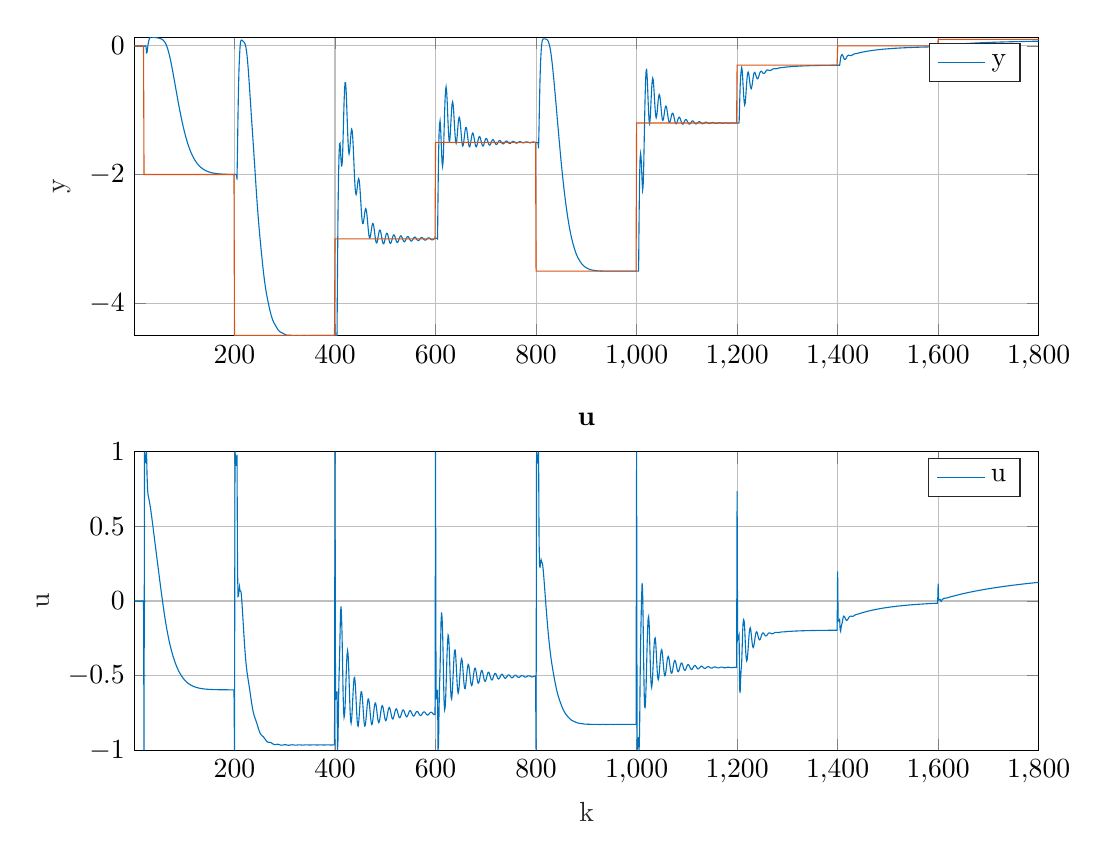
\begin{tikzpicture}

\begin{axis}[%
width=4.521in,
height=1.493in,
at={(0.758in,2.554in)},
scale only axis,
xmin=1,
xmax=1800,
ymin=-4.5047,
ymax=0.13473,
ylabel style={font=\color{white!15!black}},
ylabel={y},
axis background/.style={fill=white},
xmajorgrids,
ymajorgrids,
legend style={legend cell align=left, align=left, draw=white!15!black}
]
\addplot [color=mycolor1]
  table[row sep=crcr]{%
1	0\\
2	0\\
3	0\\
4	0\\
5	0\\
6	0\\
7	0\\
8	0\\
9	0\\
10	0\\
11	0\\
12	0\\
13	0\\
14	0\\
15	0\\
16	0\\
17	0\\
18	0\\
19	0\\
20	0\\
21	0\\
22	0\\
23	0\\
24	0\\
25	-0.10916\\
26	-0.10378\\
27	-0.042581\\
28	0.017678\\
29	0.063185\\
30	0.093814\\
31	0.11511\\
32	0.12717\\
33	0.13255\\
34	0.13443\\
35	0.13473\\
36	0.13441\\
37	0.13375\\
38	0.13296\\
39	0.13211\\
40	0.13121\\
41	0.13023\\
42	0.12918\\
43	0.12806\\
44	0.12688\\
45	0.12565\\
46	0.12436\\
47	0.123\\
48	0.12154\\
49	0.11996\\
50	0.11821\\
51	0.11624\\
52	0.11396\\
53	0.11131\\
54	0.10817\\
55	0.10443\\
56	0.099949\\
57	0.094575\\
58	0.088141\\
59	0.080466\\
60	0.071363\\
61	0.060642\\
62	0.048119\\
63	0.033621\\
64	0.016998\\
65	-0.0018695\\
66	-0.023067\\
67	-0.046636\\
68	-0.072575\\
69	-0.10084\\
70	-0.13133\\
71	-0.16394\\
72	-0.1985\\
73	-0.23483\\
74	-0.27274\\
75	-0.31205\\
76	-0.35255\\
77	-0.39406\\
78	-0.4364\\
79	-0.4794\\
80	-0.52291\\
81	-0.56678\\
82	-0.61087\\
83	-0.65505\\
84	-0.69917\\
85	-0.74313\\
86	-0.78679\\
87	-0.83004\\
88	-0.87278\\
89	-0.91492\\
90	-0.95637\\
91	-0.99705\\
92	-1.0369\\
93	-1.0759\\
94	-1.114\\
95	-1.1512\\
96	-1.1874\\
97	-1.2226\\
98	-1.2568\\
99	-1.29\\
100	-1.3222\\
101	-1.3533\\
102	-1.3834\\
103	-1.4124\\
104	-1.4403\\
105	-1.4673\\
106	-1.4932\\
107	-1.5181\\
108	-1.542\\
109	-1.5649\\
110	-1.587\\
111	-1.6081\\
112	-1.6283\\
113	-1.6476\\
114	-1.6661\\
115	-1.6838\\
116	-1.7006\\
117	-1.7167\\
118	-1.732\\
119	-1.7466\\
120	-1.7604\\
121	-1.7736\\
122	-1.7862\\
123	-1.7981\\
124	-1.8094\\
125	-1.8202\\
126	-1.8304\\
127	-1.8401\\
128	-1.8493\\
129	-1.8581\\
130	-1.8663\\
131	-1.8741\\
132	-1.8815\\
133	-1.8885\\
134	-1.895\\
135	-1.9013\\
136	-1.9071\\
137	-1.9127\\
138	-1.918\\
139	-1.9229\\
140	-1.9276\\
141	-1.932\\
142	-1.9362\\
143	-1.9401\\
144	-1.9438\\
145	-1.9473\\
146	-1.9505\\
147	-1.9536\\
148	-1.9565\\
149	-1.9592\\
150	-1.9618\\
151	-1.9642\\
152	-1.9664\\
153	-1.9686\\
154	-1.9706\\
155	-1.9724\\
156	-1.9742\\
157	-1.9759\\
158	-1.9774\\
159	-1.9789\\
160	-1.9802\\
161	-1.9815\\
162	-1.9827\\
163	-1.9838\\
164	-1.9849\\
165	-1.9858\\
166	-1.9868\\
167	-1.9876\\
168	-1.9885\\
169	-1.9892\\
170	-1.9899\\
171	-1.9906\\
172	-1.9912\\
173	-1.9918\\
174	-1.9923\\
175	-1.9928\\
176	-1.9933\\
177	-1.9938\\
178	-1.9942\\
179	-1.9946\\
180	-1.9949\\
181	-1.9953\\
182	-1.9956\\
183	-1.9959\\
184	-1.9962\\
185	-1.9964\\
186	-1.9967\\
187	-1.9969\\
188	-1.9971\\
189	-1.9973\\
190	-1.9975\\
191	-1.9977\\
192	-1.9978\\
193	-1.998\\
194	-1.9981\\
195	-1.9982\\
196	-1.9984\\
197	-1.9985\\
198	-1.9986\\
199	-1.9987\\
200	-1.9988\\
201	-1.9989\\
202	-1.9989\\
203	-1.999\\
204	-1.9991\\
205	-2.0793\\
206	-1.6006\\
207	-1.0685\\
208	-0.64917\\
209	-0.35704\\
210	-0.16617\\
211	-0.023205\\
212	0.05533\\
213	0.084477\\
214	0.089156\\
215	0.085415\\
216	0.079327\\
217	0.071835\\
218	0.064672\\
219	0.057084\\
220	0.046261\\
221	0.028904\\
222	0.0022199\\
223	-0.036168\\
224	-0.088165\\
225	-0.15464\\
226	-0.2352\\
227	-0.32845\\
228	-0.43223\\
229	-0.54389\\
230	-0.66062\\
231	-0.77989\\
232	-0.89973\\
233	-1.0189\\
234	-1.1368\\
235	-1.2537\\
236	-1.3702\\
237	-1.487\\
238	-1.6047\\
239	-1.7238\\
240	-1.8441\\
241	-1.9651\\
242	-2.0858\\
243	-2.205\\
244	-2.3214\\
245	-2.4338\\
246	-2.5413\\
247	-2.6437\\
248	-2.7407\\
249	-2.833\\
250	-2.9211\\
251	-3.006\\
252	-3.0883\\
253	-3.1687\\
254	-3.2474\\
255	-3.3244\\
256	-3.3992\\
257	-3.4713\\
258	-3.5401\\
259	-3.605\\
260	-3.6655\\
261	-3.7214\\
262	-3.773\\
263	-3.8206\\
264	-3.8649\\
265	-3.9065\\
266	-3.9462\\
267	-3.9845\\
268	-4.0217\\
269	-4.0578\\
270	-4.0928\\
271	-4.1263\\
272	-4.1578\\
273	-4.187\\
274	-4.2135\\
275	-4.2372\\
276	-4.2583\\
277	-4.277\\
278	-4.2938\\
279	-4.3092\\
280	-4.3237\\
281	-4.3377\\
282	-4.3516\\
283	-4.3654\\
284	-4.3789\\
285	-4.3919\\
286	-4.4042\\
287	-4.4153\\
288	-4.4251\\
289	-4.4333\\
290	-4.4401\\
291	-4.4456\\
292	-4.45\\
293	-4.4539\\
294	-4.4575\\
295	-4.4612\\
296	-4.4652\\
297	-4.4695\\
298	-4.474\\
299	-4.4786\\
300	-4.483\\
301	-4.4869\\
302	-4.4901\\
303	-4.4924\\
304	-4.494\\
305	-4.4947\\
306	-4.495\\
307	-4.495\\
308	-4.4949\\
309	-4.4952\\
310	-4.4958\\
311	-4.4968\\
312	-4.4982\\
313	-4.4999\\
314	-4.5015\\
315	-4.503\\
316	-4.5041\\
317	-4.5047\\
318	-4.5047\\
319	-4.5043\\
320	-4.5036\\
321	-4.5027\\
322	-4.5018\\
323	-4.5012\\
324	-4.501\\
325	-4.5011\\
326	-4.5016\\
327	-4.5023\\
328	-4.5032\\
329	-4.5039\\
330	-4.5045\\
331	-4.5046\\
332	-4.5045\\
333	-4.504\\
334	-4.5032\\
335	-4.5024\\
336	-4.5015\\
337	-4.5009\\
338	-4.5006\\
339	-4.5005\\
340	-4.5008\\
341	-4.5012\\
342	-4.5018\\
343	-4.5023\\
344	-4.5027\\
345	-4.5029\\
346	-4.5028\\
347	-4.5024\\
348	-4.5018\\
349	-4.5012\\
350	-4.5006\\
351	-4.5001\\
352	-4.4998\\
353	-4.4997\\
354	-4.4999\\
355	-4.5002\\
356	-4.5007\\
357	-4.5011\\
358	-4.5015\\
359	-4.5016\\
360	-4.5016\\
361	-4.5014\\
362	-4.501\\
363	-4.5005\\
364	-4.5001\\
365	-4.4997\\
366	-4.4994\\
367	-4.4994\\
368	-4.4995\\
369	-4.4998\\
370	-4.5002\\
371	-4.5005\\
372	-4.5008\\
373	-4.501\\
374	-4.501\\
375	-4.5008\\
376	-4.5006\\
377	-4.5002\\
378	-4.4999\\
379	-4.4996\\
380	-4.4994\\
381	-4.4994\\
382	-4.4995\\
383	-4.4997\\
384	-4.4999\\
385	-4.5002\\
386	-4.5005\\
387	-4.5006\\
388	-4.5007\\
389	-4.5006\\
390	-4.5004\\
391	-4.5001\\
392	-4.4999\\
393	-4.4997\\
394	-4.4995\\
395	-4.4995\\
396	-4.4995\\
397	-4.4997\\
398	-4.4999\\
399	-4.5001\\
400	-4.5003\\
401	-4.5004\\
402	-4.5005\\
403	-4.5004\\
404	-4.5003\\
405	-3.4284\\
406	-2.5636\\
407	-2.0198\\
408	-1.6976\\
409	-1.5235\\
410	-1.5141\\
411	-1.6356\\
412	-1.7793\\
413	-1.862\\
414	-1.8516\\
415	-1.7168\\
416	-1.4585\\
417	-1.1547\\
418	-0.88131\\
419	-0.67904\\
420	-0.57097\\
421	-0.57191\\
422	-0.67765\\
423	-0.86182\\
424	-1.0874\\
425	-1.3159\\
426	-1.5096\\
427	-1.6363\\
428	-1.6784\\
429	-1.6405\\
430	-1.5477\\
431	-1.4364\\
432	-1.3428\\
433	-1.2952\\
434	-1.3099\\
435	-1.3904\\
436	-1.528\\
437	-1.7036\\
438	-1.8921\\
439	-2.067\\
440	-2.2042\\
441	-2.287\\
442	-2.3098\\
443	-2.2799\\
444	-2.2161\\
445	-2.1435\\
446	-2.0862\\
447	-2.0632\\
448	-2.0848\\
449	-2.1521\\
450	-2.257\\
451	-2.3847\\
452	-2.5164\\
453	-2.6329\\
454	-2.7178\\
455	-2.7607\\
456	-2.7599\\
457	-2.7226\\
458	-2.6635\\
459	-2.6008\\
460	-2.552\\
461	-2.5305\\
462	-2.5432\\
463	-2.5898\\
464	-2.6634\\
465	-2.7523\\
466	-2.8417\\
467	-2.9174\\
468	-2.9676\\
469	-2.9856\\
470	-2.9713\\
471	-2.9312\\
472	-2.8769\\
473	-2.8223\\
474	-2.7802\\
475	-2.7604\\
476	-2.7673\\
477	-2.8002\\
478	-2.853\\
479	-2.9161\\
480	-2.9782\\
481	-3.0283\\
482	-3.0579\\
483	-3.0628\\
484	-3.0437\\
485	-3.0062\\
486	-2.9596\\
487	-2.9143\\
488	-2.8802\\
489	-2.8642\\
490	-2.8693\\
491	-2.8941\\
492	-2.9337\\
493	-2.9801\\
494	-3.0246\\
495	-3.0588\\
496	-3.0766\\
497	-3.0753\\
498	-3.0561\\
499	-3.0237\\
500	-2.9855\\
501	-2.9497\\
502	-2.9235\\
503	-2.9119\\
504	-2.9168\\
505	-2.9368\\
506	-2.9674\\
507	-3.0025\\
508	-3.0352\\
509	-3.0591\\
510	-3.0699\\
511	-3.0659\\
512	-3.0485\\
513	-3.0217\\
514	-2.9914\\
515	-2.9638\\
516	-2.9444\\
517	-2.9367\\
518	-2.9419\\
519	-2.9583\\
520	-2.9825\\
521	-3.0094\\
522	-3.0337\\
523	-3.0505\\
524	-3.0569\\
525	-3.0519\\
526	-3.0369\\
527	-3.0153\\
528	-2.9917\\
529	-2.9708\\
530	-2.9568\\
531	-2.9521\\
532	-2.9573\\
533	-2.971\\
534	-2.9903\\
535	-3.011\\
536	-3.029\\
537	-3.0409\\
538	-3.0445\\
539	-3.0393\\
540	-3.0267\\
541	-3.0094\\
542	-2.9912\\
543	-2.9756\\
544	-2.9656\\
545	-2.9631\\
546	-2.9681\\
547	-2.9795\\
548	-2.9948\\
549	-3.0107\\
550	-3.0241\\
551	-3.0324\\
552	-3.0342\\
553	-3.0292\\
554	-3.0188\\
555	-3.0051\\
556	-2.9911\\
557	-2.9795\\
558	-2.9726\\
559	-2.9715\\
560	-2.9762\\
561	-2.9856\\
562	-2.9976\\
563	-3.0098\\
564	-3.0197\\
565	-3.0255\\
566	-3.0261\\
567	-3.0215\\
568	-3.0129\\
569	-3.0022\\
570	-2.9915\\
571	-2.983\\
572	-2.9782\\
573	-2.9781\\
574	-2.9823\\
575	-2.99\\
576	-2.9995\\
577	-3.0088\\
578	-3.0161\\
579	-3.02\\
580	-3.0198\\
581	-3.0158\\
582	-3.0088\\
583	-3.0004\\
584	-2.9922\\
585	-2.986\\
586	-2.9828\\
587	-2.9832\\
588	-2.987\\
589	-2.9932\\
590	-3.0006\\
591	-3.0077\\
592	-3.013\\
593	-3.0156\\
594	-3.015\\
595	-3.0115\\
596	-3.0058\\
597	-2.9993\\
598	-2.9931\\
599	-2.9886\\
600	-2.9865\\
601	-2.9872\\
602	-2.9905\\
603	-2.9955\\
604	-3.0013\\
605	-2.2826\\
606	-1.6962\\
607	-1.3691\\
608	-1.2134\\
609	-1.1652\\
610	-1.2502\\
611	-1.4477\\
612	-1.6602\\
613	-1.8121\\
614	-1.8731\\
615	-1.8102\\
616	-1.6064\\
617	-1.3253\\
618	-1.0475\\
619	-0.8227\\
620	-0.67942\\
621	-0.63681\\
622	-0.69657\\
623	-0.83748\\
624	-1.0245\\
625	-1.219\\
626	-1.3821\\
627	-1.4785\\
628	-1.4867\\
629	-1.4095\\
630	-1.274\\
631	-1.1195\\
632	-0.98372\\
633	-0.89504\\
634	-0.86943\\
635	-0.90965\\
636	-1.0057\\
637	-1.1375\\
638	-1.2793\\
639	-1.4038\\
640	-1.4875\\
641	-1.5151\\
642	-1.4844\\
643	-1.4079\\
644	-1.3086\\
645	-1.2124\\
646	-1.1415\\
647	-1.1105\\
648	-1.1249\\
649	-1.1809\\
650	-1.2666\\
651	-1.3649\\
652	-1.4567\\
653	-1.5246\\
654	-1.556\\
655	-1.5469\\
656	-1.5023\\
657	-1.4357\\
658	-1.3644\\
659	-1.3052\\
660	-1.2709\\
661	-1.2681\\
662	-1.2965\\
663	-1.3496\\
664	-1.4163\\
665	-1.4831\\
666	-1.5369\\
667	-1.5675\\
668	-1.5698\\
669	-1.5452\\
670	-1.5012\\
671	-1.449\\
672	-1.401\\
673	-1.3678\\
674	-1.3558\\
675	-1.3669\\
676	-1.3981\\
677	-1.4423\\
678	-1.4903\\
679	-1.5323\\
680	-1.56\\
681	-1.5683\\
682	-1.5566\\
683	-1.5287\\
684	-1.4917\\
685	-1.4544\\
686	-1.425\\
687	-1.4094\\
688	-1.4105\\
689	-1.4273\\
690	-1.4558\\
691	-1.4896\\
692	-1.5217\\
693	-1.5455\\
694	-1.5565\\
695	-1.5529\\
696	-1.5363\\
697	-1.5111\\
698	-1.4832\\
699	-1.4589\\
700	-1.4431\\
701	-1.4389\\
702	-1.4466\\
703	-1.4641\\
704	-1.4874\\
705	-1.5113\\
706	-1.531\\
707	-1.5424\\
708	-1.5436\\
709	-1.5347\\
710	-1.5183\\
711	-1.4982\\
712	-1.479\\
713	-1.4648\\
714	-1.4583\\
715	-1.4605\\
716	-1.4705\\
717	-1.486\\
718	-1.5035\\
719	-1.5191\\
720	-1.5298\\
721	-1.5334\\
722	-1.5295\\
723	-1.5194\\
724	-1.5055\\
725	-1.491\\
726	-1.4789\\
727	-1.4719\\
728	-1.471\\
729	-1.4762\\
730	-1.4861\\
731	-1.4984\\
732	-1.5104\\
733	-1.5197\\
734	-1.5243\\
735	-1.5235\\
736	-1.5177\\
737	-1.5084\\
738	-1.4978\\
739	-1.4882\\
740	-1.4815\\
741	-1.4791\\
742	-1.4812\\
743	-1.4872\\
744	-1.4956\\
745	-1.5046\\
746	-1.5122\\
747	-1.5169\\
748	-1.5178\\
749	-1.5149\\
750	-1.509\\
751	-1.5015\\
752	-1.4941\\
753	-1.4883\\
754	-1.4853\\
755	-1.4856\\
756	-1.4889\\
757	-1.4945\\
758	-1.501\\
759	-1.507\\
760	-1.5113\\
761	-1.513\\
762	-1.5119\\
763	-1.5084\\
764	-1.5033\\
765	-1.4977\\
766	-1.493\\
767	-1.49\\
768	-1.4892\\
769	-1.4909\\
770	-1.4944\\
771	-1.4989\\
772	-1.5035\\
773	-1.5071\\
774	-1.5091\\
775	-1.5091\\
776	-1.5072\\
777	-1.5038\\
778	-1.4999\\
779	-1.4961\\
780	-1.4934\\
781	-1.4922\\
782	-1.4928\\
783	-1.4948\\
784	-1.4979\\
785	-1.5013\\
786	-1.5043\\
787	-1.5062\\
788	-1.5068\\
789	-1.5059\\
790	-1.5038\\
791	-1.501\\
792	-1.4982\\
793	-1.4959\\
794	-1.4946\\
795	-1.4945\\
796	-1.4956\\
797	-1.4976\\
798	-1.5\\
799	-1.5023\\
800	-1.504\\
801	-1.5048\\
802	-1.5046\\
803	-1.5034\\
804	-1.5015\\
805	-1.593\\
806	-1.2321\\
807	-0.81622\\
808	-0.48522\\
809	-0.25367\\
810	-0.10208\\
811	0.0057311\\
812	0.067006\\
813	0.094563\\
814	0.10473\\
815	0.10779\\
816	0.10866\\
817	0.10816\\
818	0.10726\\
819	0.10611\\
820	0.10418\\
821	0.10061\\
822	0.094558\\
823	0.085227\\
824	0.071735\\
825	0.053173\\
826	0.028705\\
827	-0.0023751\\
828	-0.040595\\
829	-0.086247\\
830	-0.13933\\
831	-0.19954\\
832	-0.2663\\
833	-0.33882\\
834	-0.41615\\
835	-0.4973\\
836	-0.58132\\
837	-0.66739\\
838	-0.75482\\
839	-0.84314\\
840	-0.932\\
841	-1.0212\\
842	-1.1106\\
843	-1.2002\\
844	-1.2897\\
845	-1.3789\\
846	-1.4676\\
847	-1.5553\\
848	-1.6418\\
849	-1.7265\\
850	-1.8091\\
851	-1.8893\\
852	-1.967\\
853	-2.042\\
854	-2.1145\\
855	-2.1844\\
856	-2.252\\
857	-2.3173\\
858	-2.3806\\
859	-2.4417\\
860	-2.5008\\
861	-2.5577\\
862	-2.6123\\
863	-2.6645\\
864	-2.7142\\
865	-2.7615\\
866	-2.8061\\
867	-2.8484\\
868	-2.8883\\
869	-2.9261\\
870	-2.9619\\
871	-2.996\\
872	-3.0285\\
873	-3.0595\\
874	-3.089\\
875	-3.117\\
876	-3.1436\\
877	-3.1686\\
878	-3.192\\
879	-3.2139\\
880	-3.2342\\
881	-3.2531\\
882	-3.2706\\
883	-3.2869\\
884	-3.3022\\
885	-3.3166\\
886	-3.3302\\
887	-3.3431\\
888	-3.3554\\
889	-3.3669\\
890	-3.3778\\
891	-3.3879\\
892	-3.3972\\
893	-3.4057\\
894	-3.4135\\
895	-3.4205\\
896	-3.4269\\
897	-3.4327\\
898	-3.4382\\
899	-3.4432\\
900	-3.448\\
901	-3.4526\\
902	-3.457\\
903	-3.4611\\
904	-3.465\\
905	-3.4686\\
906	-3.4718\\
907	-3.4746\\
908	-3.4771\\
909	-3.4793\\
910	-3.4812\\
911	-3.4828\\
912	-3.4844\\
913	-3.4858\\
914	-3.4872\\
915	-3.4886\\
916	-3.4899\\
917	-3.4913\\
918	-3.4925\\
919	-3.4937\\
920	-3.4947\\
921	-3.4955\\
922	-3.4961\\
923	-3.4966\\
924	-3.497\\
925	-3.4972\\
926	-3.4975\\
927	-3.4977\\
928	-3.498\\
929	-3.4983\\
930	-3.4987\\
931	-3.4991\\
932	-3.4995\\
933	-3.4999\\
934	-3.5002\\
935	-3.5004\\
936	-3.5005\\
937	-3.5005\\
938	-3.5004\\
939	-3.5003\\
940	-3.5002\\
941	-3.5002\\
942	-3.5002\\
943	-3.5002\\
944	-3.5003\\
945	-3.5005\\
946	-3.5006\\
947	-3.5008\\
948	-3.5009\\
949	-3.5009\\
950	-3.5009\\
951	-3.5008\\
952	-3.5007\\
953	-3.5005\\
954	-3.5004\\
955	-3.5003\\
956	-3.5002\\
957	-3.5003\\
958	-3.5003\\
959	-3.5004\\
960	-3.5005\\
961	-3.5006\\
962	-3.5006\\
963	-3.5006\\
964	-3.5006\\
965	-3.5005\\
966	-3.5004\\
967	-3.5003\\
968	-3.5002\\
969	-3.5001\\
970	-3.5001\\
971	-3.5001\\
972	-3.5001\\
973	-3.5002\\
974	-3.5002\\
975	-3.5003\\
976	-3.5004\\
977	-3.5004\\
978	-3.5003\\
979	-3.5003\\
980	-3.5002\\
981	-3.5001\\
982	-3.5\\
983	-3.5\\
984	-3.4999\\
985	-3.5\\
986	-3.5\\
987	-3.5\\
988	-3.5001\\
989	-3.5002\\
990	-3.5002\\
991	-3.5002\\
992	-3.5002\\
993	-3.5001\\
994	-3.5001\\
995	-3.5\\
996	-3.5\\
997	-3.4999\\
998	-3.4999\\
999	-3.4999\\
1000	-3.5\\
1001	-3.5\\
1002	-3.5001\\
1003	-3.5001\\
1004	-3.5001\\
1005	-2.6629\\
1006	-2.0298\\
1007	-1.7393\\
1008	-1.6721\\
1009	-1.742\\
1010	-1.9078\\
1011	-2.1128\\
1012	-2.2382\\
1013	-2.1847\\
1014	-1.9355\\
1015	-1.5503\\
1016	-1.1357\\
1017	-0.77948\\
1018	-0.52042\\
1019	-0.38047\\
1020	-0.36988\\
1021	-0.47391\\
1022	-0.65403\\
1023	-0.86292\\
1024	-1.0536\\
1025	-1.1809\\
1026	-1.2101\\
1027	-1.136\\
1028	-0.98901\\
1029	-0.81615\\
1030	-0.6595\\
1031	-0.54902\\
1032	-0.50296\\
1033	-0.52651\\
1034	-0.61062\\
1035	-0.73511\\
1036	-0.87376\\
1037	-0.99892\\
1038	-1.0858\\
1039	-1.118\\
1040	-1.0934\\
1041	-1.0245\\
1042	-0.93402\\
1043	-0.84656\\
1044	-0.78273\\
1045	-0.75581\\
1046	-0.77046\\
1047	-0.82266\\
1048	-0.90114\\
1049	-0.99002\\
1050	-1.072\\
1051	-1.1316\\
1052	-1.1585\\
1053	-1.1503\\
1054	-1.1129\\
1055	-1.0587\\
1056	-1.0028\\
1057	-0.95895\\
1058	-0.93712\\
1059	-0.94168\\
1060	-0.97129\\
1061	-1.0195\\
1062	-1.0765\\
1063	-1.1309\\
1064	-1.1723\\
1065	-1.1936\\
1066	-1.1922\\
1067	-1.1708\\
1068	-1.1365\\
1069	-1.0987\\
1070	-1.0668\\
1071	-1.0482\\
1072	-1.0466\\
1073	-1.0622\\
1074	-1.0913\\
1075	-1.1279\\
1076	-1.1643\\
1077	-1.1934\\
1078	-1.2101\\
1079	-1.2118\\
1080	-1.1996\\
1081	-1.1776\\
1082	-1.1518\\
1083	-1.1284\\
1084	-1.113\\
1085	-1.1086\\
1086	-1.116\\
1087	-1.1332\\
1088	-1.1566\\
1089	-1.181\\
1090	-1.2016\\
1091	-1.2145\\
1092	-1.2175\\
1093	-1.2109\\
1094	-1.197\\
1095	-1.1794\\
1096	-1.1626\\
1097	-1.1502\\
1098	-1.145\\
1099	-1.1478\\
1100	-1.1578\\
1101	-1.1726\\
1102	-1.189\\
1103	-1.2035\\
1104	-1.2134\\
1105	-1.2168\\
1106	-1.2136\\
1107	-1.2049\\
1108	-1.1931\\
1109	-1.1811\\
1110	-1.1716\\
1111	-1.1666\\
1112	-1.167\\
1113	-1.1726\\
1114	-1.1818\\
1115	-1.1928\\
1116	-1.203\\
1117	-1.2104\\
1118	-1.2137\\
1119	-1.2125\\
1120	-1.2072\\
1121	-1.1995\\
1122	-1.1911\\
1123	-1.184\\
1124	-1.1797\\
1125	-1.1789\\
1126	-1.1818\\
1127	-1.1875\\
1128	-1.1947\\
1129	-1.2018\\
1130	-1.2074\\
1131	-1.2103\\
1132	-1.2101\\
1133	-1.2071\\
1134	-1.2021\\
1135	-1.1963\\
1136	-1.1911\\
1137	-1.1876\\
1138	-1.1864\\
1139	-1.1878\\
1140	-1.1912\\
1141	-1.1959\\
1142	-1.2008\\
1143	-1.2049\\
1144	-1.2073\\
1145	-1.2077\\
1146	-1.206\\
1147	-1.2029\\
1148	-1.199\\
1149	-1.1952\\
1150	-1.1925\\
1151	-1.1912\\
1152	-1.1917\\
1153	-1.1937\\
1154	-1.1968\\
1155	-1.2001\\
1156	-1.2031\\
1157	-1.205\\
1158	-1.2056\\
1159	-1.2048\\
1160	-1.2028\\
1161	-1.2002\\
1162	-1.1976\\
1163	-1.1955\\
1164	-1.1943\\
1165	-1.1944\\
1166	-1.1955\\
1167	-1.1974\\
1168	-1.1997\\
1169	-1.2018\\
1170	-1.2033\\
1171	-1.2039\\
1172	-1.2036\\
1173	-1.2024\\
1174	-1.2007\\
1175	-1.1989\\
1176	-1.1973\\
1177	-1.1964\\
1178	-1.1962\\
1179	-1.1968\\
1180	-1.198\\
1181	-1.1995\\
1182	-1.201\\
1183	-1.2021\\
1184	-1.2027\\
1185	-1.2026\\
1186	-1.2019\\
1187	-1.2009\\
1188	-1.1996\\
1189	-1.1985\\
1190	-1.1977\\
1191	-1.1974\\
1192	-1.1977\\
1193	-1.1984\\
1194	-1.1994\\
1195	-1.2005\\
1196	-1.2013\\
1197	-1.2018\\
1198	-1.2019\\
1199	-1.2015\\
1200	-1.2008\\
1201	-1.2\\
1202	-1.1992\\
1203	-1.1986\\
1204	-1.1983\\
1205	-0.91371\\
1206	-0.64488\\
1207	-0.48251\\
1208	-0.38992\\
1209	-0.34075\\
1210	-0.37201\\
1211	-0.48658\\
1212	-0.63157\\
1213	-0.765\\
1214	-0.86828\\
1215	-0.91907\\
1216	-0.89628\\
1217	-0.81149\\
1218	-0.69674\\
1219	-0.58056\\
1220	-0.48427\\
1221	-0.42392\\
1222	-0.40734\\
1223	-0.43138\\
1224	-0.48443\\
1225	-0.5506\\
1226	-0.61254\\
1227	-0.65442\\
1228	-0.66608\\
1229	-0.64613\\
1230	-0.60156\\
1231	-0.54452\\
1232	-0.48815\\
1233	-0.44341\\
1234	-0.41716\\
1235	-0.41147\\
1236	-0.42382\\
1237	-0.44812\\
1238	-0.47631\\
1239	-0.50028\\
1240	-0.51374\\
1241	-0.51357\\
1242	-0.50035\\
1243	-0.47776\\
1244	-0.45121\\
1245	-0.42626\\
1246	-0.4073\\
1247	-0.39684\\
1248	-0.39518\\
1249	-0.40067\\
1250	-0.41029\\
1251	-0.42051\\
1252	-0.42808\\
1253	-0.43083\\
1254	-0.42799\\
1255	-0.42023\\
1256	-0.40931\\
1257	-0.39748\\
1258	-0.3869\\
1259	-0.37916\\
1260	-0.37498\\
1261	-0.37423\\
1262	-0.37603\\
1263	-0.37904\\
1264	-0.38188\\
1265	-0.38339\\
1266	-0.38289\\
1267	-0.38029\\
1268	-0.376\\
1269	-0.37079\\
1270	-0.36552\\
1271	-0.36097\\
1272	-0.35766\\
1273	-0.35574\\
1274	-0.35506\\
1275	-0.35522\\
1276	-0.35567\\
1277	-0.35591\\
1278	-0.35558\\
1279	-0.35448\\
1280	-0.35265\\
1281	-0.35029\\
1282	-0.34772\\
1283	-0.34525\\
1284	-0.34314\\
1285	-0.34153\\
1286	-0.34044\\
1287	-0.33977\\
1288	-0.33936\\
1289	-0.33901\\
1290	-0.33854\\
1291	-0.33784\\
1292	-0.33688\\
1293	-0.33568\\
1294	-0.33435\\
1295	-0.33299\\
1296	-0.33171\\
1297	-0.3306\\
1298	-0.32968\\
1299	-0.32895\\
1300	-0.32837\\
1301	-0.32786\\
1302	-0.32736\\
1303	-0.32681\\
1304	-0.32619\\
1305	-0.32548\\
1306	-0.3247\\
1307	-0.3239\\
1308	-0.32312\\
1309	-0.32238\\
1310	-0.32172\\
1311	-0.32113\\
1312	-0.32061\\
1313	-0.32014\\
1314	-0.3197\\
1315	-0.31926\\
1316	-0.3188\\
1317	-0.31833\\
1318	-0.31783\\
1319	-0.31732\\
1320	-0.31681\\
1321	-0.31632\\
1322	-0.31585\\
1323	-0.31542\\
1324	-0.31502\\
1325	-0.31464\\
1326	-0.31429\\
1327	-0.31395\\
1328	-0.3136\\
1329	-0.31326\\
1330	-0.31292\\
1331	-0.31257\\
1332	-0.31223\\
1333	-0.31189\\
1334	-0.31157\\
1335	-0.31125\\
1336	-0.31096\\
1337	-0.31067\\
1338	-0.3104\\
1339	-0.31014\\
1340	-0.30989\\
1341	-0.30964\\
1342	-0.30939\\
1343	-0.30915\\
1344	-0.30891\\
1345	-0.30867\\
1346	-0.30844\\
1347	-0.30821\\
1348	-0.308\\
1349	-0.30779\\
1350	-0.30759\\
1351	-0.3074\\
1352	-0.30721\\
1353	-0.30703\\
1354	-0.30685\\
1355	-0.30667\\
1356	-0.3065\\
1357	-0.30633\\
1358	-0.30616\\
1359	-0.306\\
1360	-0.30584\\
1361	-0.30569\\
1362	-0.30555\\
1363	-0.3054\\
1364	-0.30526\\
1365	-0.30513\\
1366	-0.305\\
1367	-0.30487\\
1368	-0.30474\\
1369	-0.30462\\
1370	-0.3045\\
1371	-0.30439\\
1372	-0.30427\\
1373	-0.30416\\
1374	-0.30405\\
1375	-0.30395\\
1376	-0.30385\\
1377	-0.30375\\
1378	-0.30365\\
1379	-0.30356\\
1380	-0.30347\\
1381	-0.30338\\
1382	-0.30329\\
1383	-0.30321\\
1384	-0.30312\\
1385	-0.30304\\
1386	-0.30297\\
1387	-0.30289\\
1388	-0.30281\\
1389	-0.30274\\
1390	-0.30267\\
1391	-0.3026\\
1392	-0.30254\\
1393	-0.30247\\
1394	-0.30241\\
1395	-0.30235\\
1396	-0.30229\\
1397	-0.30223\\
1398	-0.30217\\
1399	-0.30211\\
1400	-0.30206\\
1401	-0.30201\\
1402	-0.30196\\
1403	-0.30191\\
1404	-0.30186\\
1405	-0.2457\\
1406	-0.1876\\
1407	-0.15663\\
1408	-0.14195\\
1409	-0.13628\\
1410	-0.14432\\
1411	-0.16507\\
1412	-0.18716\\
1413	-0.20314\\
1414	-0.21149\\
1415	-0.21161\\
1416	-0.20357\\
1417	-0.19016\\
1418	-0.17539\\
1419	-0.16235\\
1420	-0.15274\\
1421	-0.14735\\
1422	-0.14592\\
1423	-0.14728\\
1424	-0.14977\\
1425	-0.15192\\
1426	-0.15265\\
1427	-0.15146\\
1428	-0.14843\\
1429	-0.14406\\
1430	-0.1391\\
1431	-0.13426\\
1432	-0.13006\\
1433	-0.12679\\
1434	-0.12446\\
1435	-0.12286\\
1436	-0.12168\\
1437	-0.12059\\
1438	-0.11932\\
1439	-0.11774\\
1440	-0.11581\\
1441	-0.11361\\
1442	-0.11127\\
1443	-0.10892\\
1444	-0.1067\\
1445	-0.10467\\
1446	-0.10284\\
1447	-0.10121\\
1448	-0.099697\\
1449	-0.098255\\
1450	-0.096825\\
1451	-0.095371\\
1452	-0.093881\\
1453	-0.09236\\
1454	-0.090828\\
1455	-0.08931\\
1456	-0.087828\\
1457	-0.086397\\
1458	-0.085023\\
1459	-0.083704\\
1460	-0.082431\\
1461	-0.081193\\
1462	-0.079981\\
1463	-0.078785\\
1464	-0.077602\\
1465	-0.076432\\
1466	-0.075276\\
1467	-0.074138\\
1468	-0.073022\\
1469	-0.071929\\
1470	-0.070862\\
1471	-0.069819\\
1472	-0.068799\\
1473	-0.067801\\
1474	-0.066821\\
1475	-0.065859\\
1476	-0.064914\\
1477	-0.063984\\
1478	-0.063069\\
1479	-0.06217\\
1480	-0.061287\\
1481	-0.06042\\
1482	-0.059569\\
1483	-0.058733\\
1484	-0.057913\\
1485	-0.057108\\
1486	-0.056317\\
1487	-0.055539\\
1488	-0.054775\\
1489	-0.054023\\
1490	-0.053284\\
1491	-0.052558\\
1492	-0.051844\\
1493	-0.051141\\
1494	-0.050451\\
1495	-0.049772\\
1496	-0.049104\\
1497	-0.048448\\
1498	-0.047802\\
1499	-0.047167\\
1500	-0.046542\\
1501	-0.045927\\
1502	-0.045322\\
1503	-0.044727\\
1504	-0.044141\\
1505	-0.043564\\
1506	-0.042997\\
1507	-0.042438\\
1508	-0.041889\\
1509	-0.041348\\
1510	-0.040815\\
1511	-0.04029\\
1512	-0.039774\\
1513	-0.039266\\
1514	-0.038765\\
1515	-0.038272\\
1516	-0.037786\\
1517	-0.037308\\
1518	-0.036837\\
1519	-0.036373\\
1520	-0.035916\\
1521	-0.035465\\
1522	-0.035022\\
1523	-0.034585\\
1524	-0.034154\\
1525	-0.03373\\
1526	-0.033311\\
1527	-0.032899\\
1528	-0.032493\\
1529	-0.032093\\
1530	-0.031698\\
1531	-0.03131\\
1532	-0.030926\\
1533	-0.030548\\
1534	-0.030176\\
1535	-0.029809\\
1536	-0.029447\\
1537	-0.02909\\
1538	-0.028738\\
1539	-0.028391\\
1540	-0.028049\\
1541	-0.027711\\
1542	-0.027379\\
1543	-0.027051\\
1544	-0.026727\\
1545	-0.026408\\
1546	-0.026093\\
1547	-0.025782\\
1548	-0.025476\\
1549	-0.025174\\
1550	-0.024876\\
1551	-0.024582\\
1552	-0.024292\\
1553	-0.024005\\
1554	-0.023723\\
1555	-0.023444\\
1556	-0.023169\\
1557	-0.022898\\
1558	-0.02263\\
1559	-0.022366\\
1560	-0.022105\\
1561	-0.021848\\
1562	-0.021594\\
1563	-0.021344\\
1564	-0.021096\\
1565	-0.020852\\
1566	-0.020611\\
1567	-0.020373\\
1568	-0.020138\\
1569	-0.019907\\
1570	-0.019678\\
1571	-0.019452\\
1572	-0.019229\\
1573	-0.019009\\
1574	-0.018791\\
1575	-0.018577\\
1576	-0.018365\\
1577	-0.018156\\
1578	-0.017949\\
1579	-0.017745\\
1580	-0.017544\\
1581	-0.017345\\
1582	-0.017149\\
1583	-0.016955\\
1584	-0.016763\\
1585	-0.016574\\
1586	-0.016387\\
1587	-0.016203\\
1588	-0.01602\\
1589	-0.01584\\
1590	-0.015663\\
1591	-0.015487\\
1592	-0.015314\\
1593	-0.015142\\
1594	-0.014973\\
1595	-0.014806\\
1596	-0.014641\\
1597	-0.014478\\
1598	-0.014317\\
1599	-0.014157\\
1600	-0.014\\
1601	-0.013845\\
1602	-0.013691\\
1603	-0.01354\\
1604	-0.01339\\
1605	-0.0054712\\
1606	0.0055205\\
1607	0.010407\\
1608	0.012081\\
1609	0.012269\\
1610	0.011327\\
1611	0.0092737\\
1612	0.007237\\
1613	0.0061559\\
1614	0.0060529\\
1615	0.0066931\\
1616	0.0078652\\
1617	0.009335\\
1618	0.010821\\
1619	0.012123\\
1620	0.013178\\
1621	0.014006\\
1622	0.014666\\
1623	0.015235\\
1624	0.015787\\
1625	0.016374\\
1626	0.017019\\
1627	0.017721\\
1628	0.018462\\
1629	0.019221\\
1630	0.019977\\
1631	0.020714\\
1632	0.021424\\
1633	0.022108\\
1634	0.022768\\
1635	0.023411\\
1636	0.024043\\
1637	0.024668\\
1638	0.025288\\
1639	0.025905\\
1640	0.026516\\
1641	0.027122\\
1642	0.027721\\
1643	0.028311\\
1644	0.028892\\
1645	0.029464\\
1646	0.030028\\
1647	0.030583\\
1648	0.031131\\
1649	0.031672\\
1650	0.032205\\
1651	0.032732\\
1652	0.033253\\
1653	0.033767\\
1654	0.034275\\
1655	0.034776\\
1656	0.035271\\
1657	0.035759\\
1658	0.036241\\
1659	0.036717\\
1660	0.037188\\
1661	0.037652\\
1662	0.038111\\
1663	0.038564\\
1664	0.039012\\
1665	0.039455\\
1666	0.039892\\
1667	0.040324\\
1668	0.04075\\
1669	0.041172\\
1670	0.041589\\
1671	0.042001\\
1672	0.042408\\
1673	0.04281\\
1674	0.043208\\
1675	0.043601\\
1676	0.04399\\
1677	0.044374\\
1678	0.044754\\
1679	0.04513\\
1680	0.045502\\
1681	0.045869\\
1682	0.046232\\
1683	0.046592\\
1684	0.046947\\
1685	0.047299\\
1686	0.047647\\
1687	0.047991\\
1688	0.048331\\
1689	0.048668\\
1690	0.049001\\
1691	0.04933\\
1692	0.049656\\
1693	0.049979\\
1694	0.050298\\
1695	0.050614\\
1696	0.050927\\
1697	0.051236\\
1698	0.051543\\
1699	0.051846\\
1700	0.052146\\
1701	0.052443\\
1702	0.052737\\
1703	0.053028\\
1704	0.053316\\
1705	0.053602\\
1706	0.053884\\
1707	0.054164\\
1708	0.054441\\
1709	0.054715\\
1710	0.054987\\
1711	0.055256\\
1712	0.055522\\
1713	0.055786\\
1714	0.056047\\
1715	0.056306\\
1716	0.056563\\
1717	0.056817\\
1718	0.057068\\
1719	0.057317\\
1720	0.057564\\
1721	0.057809\\
1722	0.058051\\
1723	0.058291\\
1724	0.058529\\
1725	0.058765\\
1726	0.058998\\
1727	0.05923\\
1728	0.059459\\
1729	0.059687\\
1730	0.059912\\
1731	0.060135\\
1732	0.060356\\
1733	0.060576\\
1734	0.060793\\
1735	0.061009\\
1736	0.061222\\
1737	0.061434\\
1738	0.061644\\
1739	0.061852\\
1740	0.062058\\
1741	0.062263\\
1742	0.062465\\
1743	0.062666\\
1744	0.062866\\
1745	0.063063\\
1746	0.063259\\
1747	0.063454\\
1748	0.063647\\
1749	0.063838\\
1750	0.064027\\
1751	0.064215\\
1752	0.064402\\
1753	0.064586\\
1754	0.06477\\
1755	0.064952\\
1756	0.065132\\
1757	0.065311\\
1758	0.065488\\
1759	0.065665\\
1760	0.065839\\
1761	0.066012\\
1762	0.066184\\
1763	0.066355\\
1764	0.066524\\
1765	0.066692\\
1766	0.066858\\
1767	0.067024\\
1768	0.067188\\
1769	0.06735\\
1770	0.067512\\
1771	0.067672\\
1772	0.067831\\
1773	0.067989\\
1774	0.068145\\
1775	0.0683\\
1776	0.068455\\
1777	0.068608\\
1778	0.068759\\
1779	0.06891\\
1780	0.06906\\
1781	0.069208\\
1782	0.069356\\
1783	0.069502\\
1784	0.069647\\
1785	0.069791\\
1786	0.069934\\
1787	0.070076\\
1788	0.070217\\
1789	0.070357\\
1790	0.070496\\
1791	0.070634\\
1792	0.070771\\
1793	0.070907\\
1794	0.071042\\
1795	0.071176\\
1796	0.071309\\
1797	0.071441\\
1798	0.071572\\
1799	0.071703\\
1800	0.071832\\
};
\addlegendentry{y}

\addplot [color=mycolor2, forget plot]
  table[row sep=crcr]{%
1	0\\
2	0\\
3	0\\
4	0\\
5	0\\
6	0\\
7	0\\
8	0\\
9	0\\
10	0\\
11	0\\
12	0\\
13	0\\
14	0\\
15	0\\
16	0\\
17	0\\
18	0\\
19	0\\
20	-2\\
21	-2\\
22	-2\\
23	-2\\
24	-2\\
25	-2\\
26	-2\\
27	-2\\
28	-2\\
29	-2\\
30	-2\\
31	-2\\
32	-2\\
33	-2\\
34	-2\\
35	-2\\
36	-2\\
37	-2\\
38	-2\\
39	-2\\
40	-2\\
41	-2\\
42	-2\\
43	-2\\
44	-2\\
45	-2\\
46	-2\\
47	-2\\
48	-2\\
49	-2\\
50	-2\\
51	-2\\
52	-2\\
53	-2\\
54	-2\\
55	-2\\
56	-2\\
57	-2\\
58	-2\\
59	-2\\
60	-2\\
61	-2\\
62	-2\\
63	-2\\
64	-2\\
65	-2\\
66	-2\\
67	-2\\
68	-2\\
69	-2\\
70	-2\\
71	-2\\
72	-2\\
73	-2\\
74	-2\\
75	-2\\
76	-2\\
77	-2\\
78	-2\\
79	-2\\
80	-2\\
81	-2\\
82	-2\\
83	-2\\
84	-2\\
85	-2\\
86	-2\\
87	-2\\
88	-2\\
89	-2\\
90	-2\\
91	-2\\
92	-2\\
93	-2\\
94	-2\\
95	-2\\
96	-2\\
97	-2\\
98	-2\\
99	-2\\
100	-2\\
101	-2\\
102	-2\\
103	-2\\
104	-2\\
105	-2\\
106	-2\\
107	-2\\
108	-2\\
109	-2\\
110	-2\\
111	-2\\
112	-2\\
113	-2\\
114	-2\\
115	-2\\
116	-2\\
117	-2\\
118	-2\\
119	-2\\
120	-2\\
121	-2\\
122	-2\\
123	-2\\
124	-2\\
125	-2\\
126	-2\\
127	-2\\
128	-2\\
129	-2\\
130	-2\\
131	-2\\
132	-2\\
133	-2\\
134	-2\\
135	-2\\
136	-2\\
137	-2\\
138	-2\\
139	-2\\
140	-2\\
141	-2\\
142	-2\\
143	-2\\
144	-2\\
145	-2\\
146	-2\\
147	-2\\
148	-2\\
149	-2\\
150	-2\\
151	-2\\
152	-2\\
153	-2\\
154	-2\\
155	-2\\
156	-2\\
157	-2\\
158	-2\\
159	-2\\
160	-2\\
161	-2\\
162	-2\\
163	-2\\
164	-2\\
165	-2\\
166	-2\\
167	-2\\
168	-2\\
169	-2\\
170	-2\\
171	-2\\
172	-2\\
173	-2\\
174	-2\\
175	-2\\
176	-2\\
177	-2\\
178	-2\\
179	-2\\
180	-2\\
181	-2\\
182	-2\\
183	-2\\
184	-2\\
185	-2\\
186	-2\\
187	-2\\
188	-2\\
189	-2\\
190	-2\\
191	-2\\
192	-2\\
193	-2\\
194	-2\\
195	-2\\
196	-2\\
197	-2\\
198	-2\\
199	-2\\
200	-4.5\\
201	-4.5\\
202	-4.5\\
203	-4.5\\
204	-4.5\\
205	-4.5\\
206	-4.5\\
207	-4.5\\
208	-4.5\\
209	-4.5\\
210	-4.5\\
211	-4.5\\
212	-4.5\\
213	-4.5\\
214	-4.5\\
215	-4.5\\
216	-4.5\\
217	-4.5\\
218	-4.5\\
219	-4.5\\
220	-4.5\\
221	-4.5\\
222	-4.5\\
223	-4.5\\
224	-4.5\\
225	-4.5\\
226	-4.5\\
227	-4.5\\
228	-4.5\\
229	-4.5\\
230	-4.5\\
231	-4.5\\
232	-4.5\\
233	-4.5\\
234	-4.5\\
235	-4.5\\
236	-4.5\\
237	-4.5\\
238	-4.5\\
239	-4.5\\
240	-4.5\\
241	-4.5\\
242	-4.5\\
243	-4.5\\
244	-4.5\\
245	-4.5\\
246	-4.5\\
247	-4.5\\
248	-4.5\\
249	-4.5\\
250	-4.5\\
251	-4.5\\
252	-4.5\\
253	-4.5\\
254	-4.5\\
255	-4.5\\
256	-4.5\\
257	-4.5\\
258	-4.5\\
259	-4.5\\
260	-4.5\\
261	-4.5\\
262	-4.5\\
263	-4.5\\
264	-4.5\\
265	-4.5\\
266	-4.5\\
267	-4.5\\
268	-4.5\\
269	-4.5\\
270	-4.5\\
271	-4.5\\
272	-4.5\\
273	-4.5\\
274	-4.5\\
275	-4.5\\
276	-4.5\\
277	-4.5\\
278	-4.5\\
279	-4.5\\
280	-4.5\\
281	-4.5\\
282	-4.5\\
283	-4.5\\
284	-4.5\\
285	-4.5\\
286	-4.5\\
287	-4.5\\
288	-4.5\\
289	-4.5\\
290	-4.5\\
291	-4.5\\
292	-4.5\\
293	-4.5\\
294	-4.5\\
295	-4.5\\
296	-4.5\\
297	-4.5\\
298	-4.5\\
299	-4.5\\
300	-4.5\\
301	-4.5\\
302	-4.5\\
303	-4.5\\
304	-4.5\\
305	-4.5\\
306	-4.5\\
307	-4.5\\
308	-4.5\\
309	-4.5\\
310	-4.5\\
311	-4.5\\
312	-4.5\\
313	-4.5\\
314	-4.5\\
315	-4.5\\
316	-4.5\\
317	-4.5\\
318	-4.5\\
319	-4.5\\
320	-4.5\\
321	-4.5\\
322	-4.5\\
323	-4.5\\
324	-4.5\\
325	-4.5\\
326	-4.5\\
327	-4.5\\
328	-4.5\\
329	-4.5\\
330	-4.5\\
331	-4.5\\
332	-4.5\\
333	-4.5\\
334	-4.5\\
335	-4.5\\
336	-4.5\\
337	-4.5\\
338	-4.5\\
339	-4.5\\
340	-4.5\\
341	-4.5\\
342	-4.5\\
343	-4.5\\
344	-4.5\\
345	-4.5\\
346	-4.5\\
347	-4.5\\
348	-4.5\\
349	-4.5\\
350	-4.5\\
351	-4.5\\
352	-4.5\\
353	-4.5\\
354	-4.5\\
355	-4.5\\
356	-4.5\\
357	-4.5\\
358	-4.5\\
359	-4.5\\
360	-4.5\\
361	-4.5\\
362	-4.5\\
363	-4.5\\
364	-4.5\\
365	-4.5\\
366	-4.5\\
367	-4.5\\
368	-4.5\\
369	-4.5\\
370	-4.5\\
371	-4.5\\
372	-4.5\\
373	-4.5\\
374	-4.5\\
375	-4.5\\
376	-4.5\\
377	-4.5\\
378	-4.5\\
379	-4.5\\
380	-4.5\\
381	-4.5\\
382	-4.5\\
383	-4.5\\
384	-4.5\\
385	-4.5\\
386	-4.5\\
387	-4.5\\
388	-4.5\\
389	-4.5\\
390	-4.5\\
391	-4.5\\
392	-4.5\\
393	-4.5\\
394	-4.5\\
395	-4.5\\
396	-4.5\\
397	-4.5\\
398	-4.5\\
399	-4.5\\
400	-3\\
401	-3\\
402	-3\\
403	-3\\
404	-3\\
405	-3\\
406	-3\\
407	-3\\
408	-3\\
409	-3\\
410	-3\\
411	-3\\
412	-3\\
413	-3\\
414	-3\\
415	-3\\
416	-3\\
417	-3\\
418	-3\\
419	-3\\
420	-3\\
421	-3\\
422	-3\\
423	-3\\
424	-3\\
425	-3\\
426	-3\\
427	-3\\
428	-3\\
429	-3\\
430	-3\\
431	-3\\
432	-3\\
433	-3\\
434	-3\\
435	-3\\
436	-3\\
437	-3\\
438	-3\\
439	-3\\
440	-3\\
441	-3\\
442	-3\\
443	-3\\
444	-3\\
445	-3\\
446	-3\\
447	-3\\
448	-3\\
449	-3\\
450	-3\\
451	-3\\
452	-3\\
453	-3\\
454	-3\\
455	-3\\
456	-3\\
457	-3\\
458	-3\\
459	-3\\
460	-3\\
461	-3\\
462	-3\\
463	-3\\
464	-3\\
465	-3\\
466	-3\\
467	-3\\
468	-3\\
469	-3\\
470	-3\\
471	-3\\
472	-3\\
473	-3\\
474	-3\\
475	-3\\
476	-3\\
477	-3\\
478	-3\\
479	-3\\
480	-3\\
481	-3\\
482	-3\\
483	-3\\
484	-3\\
485	-3\\
486	-3\\
487	-3\\
488	-3\\
489	-3\\
490	-3\\
491	-3\\
492	-3\\
493	-3\\
494	-3\\
495	-3\\
496	-3\\
497	-3\\
498	-3\\
499	-3\\
500	-3\\
501	-3\\
502	-3\\
503	-3\\
504	-3\\
505	-3\\
506	-3\\
507	-3\\
508	-3\\
509	-3\\
510	-3\\
511	-3\\
512	-3\\
513	-3\\
514	-3\\
515	-3\\
516	-3\\
517	-3\\
518	-3\\
519	-3\\
520	-3\\
521	-3\\
522	-3\\
523	-3\\
524	-3\\
525	-3\\
526	-3\\
527	-3\\
528	-3\\
529	-3\\
530	-3\\
531	-3\\
532	-3\\
533	-3\\
534	-3\\
535	-3\\
536	-3\\
537	-3\\
538	-3\\
539	-3\\
540	-3\\
541	-3\\
542	-3\\
543	-3\\
544	-3\\
545	-3\\
546	-3\\
547	-3\\
548	-3\\
549	-3\\
550	-3\\
551	-3\\
552	-3\\
553	-3\\
554	-3\\
555	-3\\
556	-3\\
557	-3\\
558	-3\\
559	-3\\
560	-3\\
561	-3\\
562	-3\\
563	-3\\
564	-3\\
565	-3\\
566	-3\\
567	-3\\
568	-3\\
569	-3\\
570	-3\\
571	-3\\
572	-3\\
573	-3\\
574	-3\\
575	-3\\
576	-3\\
577	-3\\
578	-3\\
579	-3\\
580	-3\\
581	-3\\
582	-3\\
583	-3\\
584	-3\\
585	-3\\
586	-3\\
587	-3\\
588	-3\\
589	-3\\
590	-3\\
591	-3\\
592	-3\\
593	-3\\
594	-3\\
595	-3\\
596	-3\\
597	-3\\
598	-3\\
599	-3\\
600	-1.5\\
601	-1.5\\
602	-1.5\\
603	-1.5\\
604	-1.5\\
605	-1.5\\
606	-1.5\\
607	-1.5\\
608	-1.5\\
609	-1.5\\
610	-1.5\\
611	-1.5\\
612	-1.5\\
613	-1.5\\
614	-1.5\\
615	-1.5\\
616	-1.5\\
617	-1.5\\
618	-1.5\\
619	-1.5\\
620	-1.5\\
621	-1.5\\
622	-1.5\\
623	-1.5\\
624	-1.5\\
625	-1.5\\
626	-1.5\\
627	-1.5\\
628	-1.5\\
629	-1.5\\
630	-1.5\\
631	-1.5\\
632	-1.5\\
633	-1.5\\
634	-1.5\\
635	-1.5\\
636	-1.5\\
637	-1.5\\
638	-1.5\\
639	-1.5\\
640	-1.5\\
641	-1.5\\
642	-1.5\\
643	-1.5\\
644	-1.5\\
645	-1.5\\
646	-1.5\\
647	-1.5\\
648	-1.5\\
649	-1.5\\
650	-1.5\\
651	-1.5\\
652	-1.5\\
653	-1.5\\
654	-1.5\\
655	-1.5\\
656	-1.5\\
657	-1.5\\
658	-1.5\\
659	-1.5\\
660	-1.5\\
661	-1.5\\
662	-1.5\\
663	-1.5\\
664	-1.5\\
665	-1.5\\
666	-1.5\\
667	-1.5\\
668	-1.5\\
669	-1.5\\
670	-1.5\\
671	-1.5\\
672	-1.5\\
673	-1.5\\
674	-1.5\\
675	-1.5\\
676	-1.5\\
677	-1.5\\
678	-1.5\\
679	-1.5\\
680	-1.5\\
681	-1.5\\
682	-1.5\\
683	-1.5\\
684	-1.5\\
685	-1.5\\
686	-1.5\\
687	-1.5\\
688	-1.5\\
689	-1.5\\
690	-1.5\\
691	-1.5\\
692	-1.5\\
693	-1.5\\
694	-1.5\\
695	-1.5\\
696	-1.5\\
697	-1.5\\
698	-1.5\\
699	-1.5\\
700	-1.5\\
701	-1.5\\
702	-1.5\\
703	-1.5\\
704	-1.5\\
705	-1.5\\
706	-1.5\\
707	-1.5\\
708	-1.5\\
709	-1.5\\
710	-1.5\\
711	-1.5\\
712	-1.5\\
713	-1.5\\
714	-1.5\\
715	-1.5\\
716	-1.5\\
717	-1.5\\
718	-1.5\\
719	-1.5\\
720	-1.5\\
721	-1.5\\
722	-1.5\\
723	-1.5\\
724	-1.5\\
725	-1.5\\
726	-1.5\\
727	-1.5\\
728	-1.5\\
729	-1.5\\
730	-1.5\\
731	-1.5\\
732	-1.5\\
733	-1.5\\
734	-1.5\\
735	-1.5\\
736	-1.5\\
737	-1.5\\
738	-1.5\\
739	-1.5\\
740	-1.5\\
741	-1.5\\
742	-1.5\\
743	-1.5\\
744	-1.5\\
745	-1.5\\
746	-1.5\\
747	-1.5\\
748	-1.5\\
749	-1.5\\
750	-1.5\\
751	-1.5\\
752	-1.5\\
753	-1.5\\
754	-1.5\\
755	-1.5\\
756	-1.5\\
757	-1.5\\
758	-1.5\\
759	-1.5\\
760	-1.5\\
761	-1.5\\
762	-1.5\\
763	-1.5\\
764	-1.5\\
765	-1.5\\
766	-1.5\\
767	-1.5\\
768	-1.5\\
769	-1.5\\
770	-1.5\\
771	-1.5\\
772	-1.5\\
773	-1.5\\
774	-1.5\\
775	-1.5\\
776	-1.5\\
777	-1.5\\
778	-1.5\\
779	-1.5\\
780	-1.5\\
781	-1.5\\
782	-1.5\\
783	-1.5\\
784	-1.5\\
785	-1.5\\
786	-1.5\\
787	-1.5\\
788	-1.5\\
789	-1.5\\
790	-1.5\\
791	-1.5\\
792	-1.5\\
793	-1.5\\
794	-1.5\\
795	-1.5\\
796	-1.5\\
797	-1.5\\
798	-1.5\\
799	-1.5\\
800	-3.5\\
801	-3.5\\
802	-3.5\\
803	-3.5\\
804	-3.5\\
805	-3.5\\
806	-3.5\\
807	-3.5\\
808	-3.5\\
809	-3.5\\
810	-3.5\\
811	-3.5\\
812	-3.5\\
813	-3.5\\
814	-3.5\\
815	-3.5\\
816	-3.5\\
817	-3.5\\
818	-3.5\\
819	-3.5\\
820	-3.5\\
821	-3.5\\
822	-3.5\\
823	-3.5\\
824	-3.5\\
825	-3.5\\
826	-3.5\\
827	-3.5\\
828	-3.5\\
829	-3.5\\
830	-3.5\\
831	-3.5\\
832	-3.5\\
833	-3.5\\
834	-3.5\\
835	-3.5\\
836	-3.5\\
837	-3.5\\
838	-3.5\\
839	-3.5\\
840	-3.5\\
841	-3.5\\
842	-3.5\\
843	-3.5\\
844	-3.5\\
845	-3.5\\
846	-3.5\\
847	-3.5\\
848	-3.5\\
849	-3.5\\
850	-3.5\\
851	-3.5\\
852	-3.5\\
853	-3.5\\
854	-3.5\\
855	-3.5\\
856	-3.5\\
857	-3.5\\
858	-3.5\\
859	-3.5\\
860	-3.5\\
861	-3.5\\
862	-3.5\\
863	-3.5\\
864	-3.5\\
865	-3.5\\
866	-3.5\\
867	-3.5\\
868	-3.5\\
869	-3.5\\
870	-3.5\\
871	-3.5\\
872	-3.5\\
873	-3.5\\
874	-3.5\\
875	-3.5\\
876	-3.5\\
877	-3.5\\
878	-3.5\\
879	-3.5\\
880	-3.5\\
881	-3.5\\
882	-3.5\\
883	-3.5\\
884	-3.5\\
885	-3.5\\
886	-3.5\\
887	-3.5\\
888	-3.5\\
889	-3.5\\
890	-3.5\\
891	-3.5\\
892	-3.5\\
893	-3.5\\
894	-3.5\\
895	-3.5\\
896	-3.5\\
897	-3.5\\
898	-3.5\\
899	-3.5\\
900	-3.5\\
901	-3.5\\
902	-3.5\\
903	-3.5\\
904	-3.5\\
905	-3.5\\
906	-3.5\\
907	-3.5\\
908	-3.5\\
909	-3.5\\
910	-3.5\\
911	-3.5\\
912	-3.5\\
913	-3.5\\
914	-3.5\\
915	-3.5\\
916	-3.5\\
917	-3.5\\
918	-3.5\\
919	-3.5\\
920	-3.5\\
921	-3.5\\
922	-3.5\\
923	-3.5\\
924	-3.5\\
925	-3.5\\
926	-3.5\\
927	-3.5\\
928	-3.5\\
929	-3.5\\
930	-3.5\\
931	-3.5\\
932	-3.5\\
933	-3.5\\
934	-3.5\\
935	-3.5\\
936	-3.5\\
937	-3.5\\
938	-3.5\\
939	-3.5\\
940	-3.5\\
941	-3.5\\
942	-3.5\\
943	-3.5\\
944	-3.5\\
945	-3.5\\
946	-3.5\\
947	-3.5\\
948	-3.5\\
949	-3.5\\
950	-3.5\\
951	-3.5\\
952	-3.5\\
953	-3.5\\
954	-3.5\\
955	-3.5\\
956	-3.5\\
957	-3.5\\
958	-3.5\\
959	-3.5\\
960	-3.5\\
961	-3.5\\
962	-3.5\\
963	-3.5\\
964	-3.5\\
965	-3.5\\
966	-3.5\\
967	-3.5\\
968	-3.5\\
969	-3.5\\
970	-3.5\\
971	-3.5\\
972	-3.5\\
973	-3.5\\
974	-3.5\\
975	-3.5\\
976	-3.5\\
977	-3.5\\
978	-3.5\\
979	-3.5\\
980	-3.5\\
981	-3.5\\
982	-3.5\\
983	-3.5\\
984	-3.5\\
985	-3.5\\
986	-3.5\\
987	-3.5\\
988	-3.5\\
989	-3.5\\
990	-3.5\\
991	-3.5\\
992	-3.5\\
993	-3.5\\
994	-3.5\\
995	-3.5\\
996	-3.5\\
997	-3.5\\
998	-3.5\\
999	-3.5\\
1000	-1.2\\
1001	-1.2\\
1002	-1.2\\
1003	-1.2\\
1004	-1.2\\
1005	-1.2\\
1006	-1.2\\
1007	-1.2\\
1008	-1.2\\
1009	-1.2\\
1010	-1.2\\
1011	-1.2\\
1012	-1.2\\
1013	-1.2\\
1014	-1.2\\
1015	-1.2\\
1016	-1.2\\
1017	-1.2\\
1018	-1.2\\
1019	-1.2\\
1020	-1.2\\
1021	-1.2\\
1022	-1.2\\
1023	-1.2\\
1024	-1.2\\
1025	-1.2\\
1026	-1.2\\
1027	-1.2\\
1028	-1.2\\
1029	-1.2\\
1030	-1.2\\
1031	-1.2\\
1032	-1.2\\
1033	-1.2\\
1034	-1.2\\
1035	-1.2\\
1036	-1.2\\
1037	-1.2\\
1038	-1.2\\
1039	-1.2\\
1040	-1.2\\
1041	-1.2\\
1042	-1.2\\
1043	-1.2\\
1044	-1.2\\
1045	-1.2\\
1046	-1.2\\
1047	-1.2\\
1048	-1.2\\
1049	-1.2\\
1050	-1.2\\
1051	-1.2\\
1052	-1.2\\
1053	-1.2\\
1054	-1.2\\
1055	-1.2\\
1056	-1.2\\
1057	-1.2\\
1058	-1.2\\
1059	-1.2\\
1060	-1.2\\
1061	-1.2\\
1062	-1.2\\
1063	-1.2\\
1064	-1.2\\
1065	-1.2\\
1066	-1.2\\
1067	-1.2\\
1068	-1.2\\
1069	-1.2\\
1070	-1.2\\
1071	-1.2\\
1072	-1.2\\
1073	-1.2\\
1074	-1.2\\
1075	-1.2\\
1076	-1.2\\
1077	-1.2\\
1078	-1.2\\
1079	-1.2\\
1080	-1.2\\
1081	-1.2\\
1082	-1.2\\
1083	-1.2\\
1084	-1.2\\
1085	-1.2\\
1086	-1.2\\
1087	-1.2\\
1088	-1.2\\
1089	-1.2\\
1090	-1.2\\
1091	-1.2\\
1092	-1.2\\
1093	-1.2\\
1094	-1.2\\
1095	-1.2\\
1096	-1.2\\
1097	-1.2\\
1098	-1.2\\
1099	-1.2\\
1100	-1.2\\
1101	-1.2\\
1102	-1.2\\
1103	-1.2\\
1104	-1.2\\
1105	-1.2\\
1106	-1.2\\
1107	-1.2\\
1108	-1.2\\
1109	-1.2\\
1110	-1.2\\
1111	-1.2\\
1112	-1.2\\
1113	-1.2\\
1114	-1.2\\
1115	-1.2\\
1116	-1.2\\
1117	-1.2\\
1118	-1.2\\
1119	-1.2\\
1120	-1.2\\
1121	-1.2\\
1122	-1.2\\
1123	-1.2\\
1124	-1.2\\
1125	-1.2\\
1126	-1.2\\
1127	-1.2\\
1128	-1.2\\
1129	-1.2\\
1130	-1.2\\
1131	-1.2\\
1132	-1.2\\
1133	-1.2\\
1134	-1.2\\
1135	-1.2\\
1136	-1.2\\
1137	-1.2\\
1138	-1.2\\
1139	-1.2\\
1140	-1.2\\
1141	-1.2\\
1142	-1.2\\
1143	-1.2\\
1144	-1.2\\
1145	-1.2\\
1146	-1.2\\
1147	-1.2\\
1148	-1.2\\
1149	-1.2\\
1150	-1.2\\
1151	-1.2\\
1152	-1.2\\
1153	-1.2\\
1154	-1.2\\
1155	-1.2\\
1156	-1.2\\
1157	-1.2\\
1158	-1.2\\
1159	-1.2\\
1160	-1.2\\
1161	-1.2\\
1162	-1.2\\
1163	-1.2\\
1164	-1.2\\
1165	-1.2\\
1166	-1.2\\
1167	-1.2\\
1168	-1.2\\
1169	-1.2\\
1170	-1.2\\
1171	-1.2\\
1172	-1.2\\
1173	-1.2\\
1174	-1.2\\
1175	-1.2\\
1176	-1.2\\
1177	-1.2\\
1178	-1.2\\
1179	-1.2\\
1180	-1.2\\
1181	-1.2\\
1182	-1.2\\
1183	-1.2\\
1184	-1.2\\
1185	-1.2\\
1186	-1.2\\
1187	-1.2\\
1188	-1.2\\
1189	-1.2\\
1190	-1.2\\
1191	-1.2\\
1192	-1.2\\
1193	-1.2\\
1194	-1.2\\
1195	-1.2\\
1196	-1.2\\
1197	-1.2\\
1198	-1.2\\
1199	-1.2\\
1200	-0.3\\
1201	-0.3\\
1202	-0.3\\
1203	-0.3\\
1204	-0.3\\
1205	-0.3\\
1206	-0.3\\
1207	-0.3\\
1208	-0.3\\
1209	-0.3\\
1210	-0.3\\
1211	-0.3\\
1212	-0.3\\
1213	-0.3\\
1214	-0.3\\
1215	-0.3\\
1216	-0.3\\
1217	-0.3\\
1218	-0.3\\
1219	-0.3\\
1220	-0.3\\
1221	-0.3\\
1222	-0.3\\
1223	-0.3\\
1224	-0.3\\
1225	-0.3\\
1226	-0.3\\
1227	-0.3\\
1228	-0.3\\
1229	-0.3\\
1230	-0.3\\
1231	-0.3\\
1232	-0.3\\
1233	-0.3\\
1234	-0.3\\
1235	-0.3\\
1236	-0.3\\
1237	-0.3\\
1238	-0.3\\
1239	-0.3\\
1240	-0.3\\
1241	-0.3\\
1242	-0.3\\
1243	-0.3\\
1244	-0.3\\
1245	-0.3\\
1246	-0.3\\
1247	-0.3\\
1248	-0.3\\
1249	-0.3\\
1250	-0.3\\
1251	-0.3\\
1252	-0.3\\
1253	-0.3\\
1254	-0.3\\
1255	-0.3\\
1256	-0.3\\
1257	-0.3\\
1258	-0.3\\
1259	-0.3\\
1260	-0.3\\
1261	-0.3\\
1262	-0.3\\
1263	-0.3\\
1264	-0.3\\
1265	-0.3\\
1266	-0.3\\
1267	-0.3\\
1268	-0.3\\
1269	-0.3\\
1270	-0.3\\
1271	-0.3\\
1272	-0.3\\
1273	-0.3\\
1274	-0.3\\
1275	-0.3\\
1276	-0.3\\
1277	-0.3\\
1278	-0.3\\
1279	-0.3\\
1280	-0.3\\
1281	-0.3\\
1282	-0.3\\
1283	-0.3\\
1284	-0.3\\
1285	-0.3\\
1286	-0.3\\
1287	-0.3\\
1288	-0.3\\
1289	-0.3\\
1290	-0.3\\
1291	-0.3\\
1292	-0.3\\
1293	-0.3\\
1294	-0.3\\
1295	-0.3\\
1296	-0.3\\
1297	-0.3\\
1298	-0.3\\
1299	-0.3\\
1300	-0.3\\
1301	-0.3\\
1302	-0.3\\
1303	-0.3\\
1304	-0.3\\
1305	-0.3\\
1306	-0.3\\
1307	-0.3\\
1308	-0.3\\
1309	-0.3\\
1310	-0.3\\
1311	-0.3\\
1312	-0.3\\
1313	-0.3\\
1314	-0.3\\
1315	-0.3\\
1316	-0.3\\
1317	-0.3\\
1318	-0.3\\
1319	-0.3\\
1320	-0.3\\
1321	-0.3\\
1322	-0.3\\
1323	-0.3\\
1324	-0.3\\
1325	-0.3\\
1326	-0.3\\
1327	-0.3\\
1328	-0.3\\
1329	-0.3\\
1330	-0.3\\
1331	-0.3\\
1332	-0.3\\
1333	-0.3\\
1334	-0.3\\
1335	-0.3\\
1336	-0.3\\
1337	-0.3\\
1338	-0.3\\
1339	-0.3\\
1340	-0.3\\
1341	-0.3\\
1342	-0.3\\
1343	-0.3\\
1344	-0.3\\
1345	-0.3\\
1346	-0.3\\
1347	-0.3\\
1348	-0.3\\
1349	-0.3\\
1350	-0.3\\
1351	-0.3\\
1352	-0.3\\
1353	-0.3\\
1354	-0.3\\
1355	-0.3\\
1356	-0.3\\
1357	-0.3\\
1358	-0.3\\
1359	-0.3\\
1360	-0.3\\
1361	-0.3\\
1362	-0.3\\
1363	-0.3\\
1364	-0.3\\
1365	-0.3\\
1366	-0.3\\
1367	-0.3\\
1368	-0.3\\
1369	-0.3\\
1370	-0.3\\
1371	-0.3\\
1372	-0.3\\
1373	-0.3\\
1374	-0.3\\
1375	-0.3\\
1376	-0.3\\
1377	-0.3\\
1378	-0.3\\
1379	-0.3\\
1380	-0.3\\
1381	-0.3\\
1382	-0.3\\
1383	-0.3\\
1384	-0.3\\
1385	-0.3\\
1386	-0.3\\
1387	-0.3\\
1388	-0.3\\
1389	-0.3\\
1390	-0.3\\
1391	-0.3\\
1392	-0.3\\
1393	-0.3\\
1394	-0.3\\
1395	-0.3\\
1396	-0.3\\
1397	-0.3\\
1398	-0.3\\
1399	-0.3\\
1400	0\\
1401	0\\
1402	0\\
1403	0\\
1404	0\\
1405	0\\
1406	0\\
1407	0\\
1408	0\\
1409	0\\
1410	0\\
1411	0\\
1412	0\\
1413	0\\
1414	0\\
1415	0\\
1416	0\\
1417	0\\
1418	0\\
1419	0\\
1420	0\\
1421	0\\
1422	0\\
1423	0\\
1424	0\\
1425	0\\
1426	0\\
1427	0\\
1428	0\\
1429	0\\
1430	0\\
1431	0\\
1432	0\\
1433	0\\
1434	0\\
1435	0\\
1436	0\\
1437	0\\
1438	0\\
1439	0\\
1440	0\\
1441	0\\
1442	0\\
1443	0\\
1444	0\\
1445	0\\
1446	0\\
1447	0\\
1448	0\\
1449	0\\
1450	0\\
1451	0\\
1452	0\\
1453	0\\
1454	0\\
1455	0\\
1456	0\\
1457	0\\
1458	0\\
1459	0\\
1460	0\\
1461	0\\
1462	0\\
1463	0\\
1464	0\\
1465	0\\
1466	0\\
1467	0\\
1468	0\\
1469	0\\
1470	0\\
1471	0\\
1472	0\\
1473	0\\
1474	0\\
1475	0\\
1476	0\\
1477	0\\
1478	0\\
1479	0\\
1480	0\\
1481	0\\
1482	0\\
1483	0\\
1484	0\\
1485	0\\
1486	0\\
1487	0\\
1488	0\\
1489	0\\
1490	0\\
1491	0\\
1492	0\\
1493	0\\
1494	0\\
1495	0\\
1496	0\\
1497	0\\
1498	0\\
1499	0\\
1500	0\\
1501	0\\
1502	0\\
1503	0\\
1504	0\\
1505	0\\
1506	0\\
1507	0\\
1508	0\\
1509	0\\
1510	0\\
1511	0\\
1512	0\\
1513	0\\
1514	0\\
1515	0\\
1516	0\\
1517	0\\
1518	0\\
1519	0\\
1520	0\\
1521	0\\
1522	0\\
1523	0\\
1524	0\\
1525	0\\
1526	0\\
1527	0\\
1528	0\\
1529	0\\
1530	0\\
1531	0\\
1532	0\\
1533	0\\
1534	0\\
1535	0\\
1536	0\\
1537	0\\
1538	0\\
1539	0\\
1540	0\\
1541	0\\
1542	0\\
1543	0\\
1544	0\\
1545	0\\
1546	0\\
1547	0\\
1548	0\\
1549	0\\
1550	0\\
1551	0\\
1552	0\\
1553	0\\
1554	0\\
1555	0\\
1556	0\\
1557	0\\
1558	0\\
1559	0\\
1560	0\\
1561	0\\
1562	0\\
1563	0\\
1564	0\\
1565	0\\
1566	0\\
1567	0\\
1568	0\\
1569	0\\
1570	0\\
1571	0\\
1572	0\\
1573	0\\
1574	0\\
1575	0\\
1576	0\\
1577	0\\
1578	0\\
1579	0\\
1580	0\\
1581	0\\
1582	0\\
1583	0\\
1584	0\\
1585	0\\
1586	0\\
1587	0\\
1588	0\\
1589	0\\
1590	0\\
1591	0\\
1592	0\\
1593	0\\
1594	0\\
1595	0\\
1596	0\\
1597	0\\
1598	0\\
1599	0\\
1600	0.1\\
1601	0.1\\
1602	0.1\\
1603	0.1\\
1604	0.1\\
1605	0.1\\
1606	0.1\\
1607	0.1\\
1608	0.1\\
1609	0.1\\
1610	0.1\\
1611	0.1\\
1612	0.1\\
1613	0.1\\
1614	0.1\\
1615	0.1\\
1616	0.1\\
1617	0.1\\
1618	0.1\\
1619	0.1\\
1620	0.1\\
1621	0.1\\
1622	0.1\\
1623	0.1\\
1624	0.1\\
1625	0.1\\
1626	0.1\\
1627	0.1\\
1628	0.1\\
1629	0.1\\
1630	0.1\\
1631	0.1\\
1632	0.1\\
1633	0.1\\
1634	0.1\\
1635	0.1\\
1636	0.1\\
1637	0.1\\
1638	0.1\\
1639	0.1\\
1640	0.1\\
1641	0.1\\
1642	0.1\\
1643	0.1\\
1644	0.1\\
1645	0.1\\
1646	0.1\\
1647	0.1\\
1648	0.1\\
1649	0.1\\
1650	0.1\\
1651	0.1\\
1652	0.1\\
1653	0.1\\
1654	0.1\\
1655	0.1\\
1656	0.1\\
1657	0.1\\
1658	0.1\\
1659	0.1\\
1660	0.1\\
1661	0.1\\
1662	0.1\\
1663	0.1\\
1664	0.1\\
1665	0.1\\
1666	0.1\\
1667	0.1\\
1668	0.1\\
1669	0.1\\
1670	0.1\\
1671	0.1\\
1672	0.1\\
1673	0.1\\
1674	0.1\\
1675	0.1\\
1676	0.1\\
1677	0.1\\
1678	0.1\\
1679	0.1\\
1680	0.1\\
1681	0.1\\
1682	0.1\\
1683	0.1\\
1684	0.1\\
1685	0.1\\
1686	0.1\\
1687	0.1\\
1688	0.1\\
1689	0.1\\
1690	0.1\\
1691	0.1\\
1692	0.1\\
1693	0.1\\
1694	0.1\\
1695	0.1\\
1696	0.1\\
1697	0.1\\
1698	0.1\\
1699	0.1\\
1700	0.1\\
1701	0.1\\
1702	0.1\\
1703	0.1\\
1704	0.1\\
1705	0.1\\
1706	0.1\\
1707	0.1\\
1708	0.1\\
1709	0.1\\
1710	0.1\\
1711	0.1\\
1712	0.1\\
1713	0.1\\
1714	0.1\\
1715	0.1\\
1716	0.1\\
1717	0.1\\
1718	0.1\\
1719	0.1\\
1720	0.1\\
1721	0.1\\
1722	0.1\\
1723	0.1\\
1724	0.1\\
1725	0.1\\
1726	0.1\\
1727	0.1\\
1728	0.1\\
1729	0.1\\
1730	0.1\\
1731	0.1\\
1732	0.1\\
1733	0.1\\
1734	0.1\\
1735	0.1\\
1736	0.1\\
1737	0.1\\
1738	0.1\\
1739	0.1\\
1740	0.1\\
1741	0.1\\
1742	0.1\\
1743	0.1\\
1744	0.1\\
1745	0.1\\
1746	0.1\\
1747	0.1\\
1748	0.1\\
1749	0.1\\
1750	0.1\\
1751	0.1\\
1752	0.1\\
1753	0.1\\
1754	0.1\\
1755	0.1\\
1756	0.1\\
1757	0.1\\
1758	0.1\\
1759	0.1\\
1760	0.1\\
1761	0.1\\
1762	0.1\\
1763	0.1\\
1764	0.1\\
1765	0.1\\
1766	0.1\\
1767	0.1\\
1768	0.1\\
1769	0.1\\
1770	0.1\\
1771	0.1\\
1772	0.1\\
1773	0.1\\
1774	0.1\\
1775	0.1\\
1776	0.1\\
1777	0.1\\
1778	0.1\\
1779	0.1\\
1780	0.1\\
1781	0.1\\
1782	0.1\\
1783	0.1\\
1784	0.1\\
1785	0.1\\
1786	0.1\\
1787	0.1\\
1788	0.1\\
1789	0.1\\
1790	0.1\\
1791	0.1\\
1792	0.1\\
1793	0.1\\
1794	0.1\\
1795	0.1\\
1796	0.1\\
1797	0.1\\
1798	0.1\\
1799	0.1\\
1800	0.1\\
};
\end{axis}

\begin{axis}[%
width=4.521in,
height=1.493in,
at={(0.758in,0.481in)},
scale only axis,
xmin=1,
xmax=1800,
xlabel style={font=\color{white!15!black}},
xlabel={k},
ymin=-1,
ymax=1,
ylabel style={font=\color{white!15!black}},
ylabel={u},
axis background/.style={fill=white},
title style={font=\bfseries},
title={u},
xmajorgrids,
ymajorgrids,
legend style={legend cell align=left, align=left, draw=white!15!black}
]
\addplot [color=mycolor1]
  table[row sep=crcr]{%
1	0\\
2	0\\
3	0\\
4	0\\
5	0\\
6	0\\
7	0\\
8	0\\
9	0\\
10	0\\
11	0\\
12	0\\
13	0\\
14	0\\
15	0\\
16	0\\
17	0\\
18	0\\
19	0\\
20	-1\\
21	1\\
22	0.97466\\
23	0.94932\\
24	0.92397\\
25	1\\
26	0.8466\\
27	0.74829\\
28	0.71301\\
29	0.69527\\
30	0.67995\\
31	0.6598\\
32	0.64106\\
33	0.62055\\
34	0.5971\\
35	0.57177\\
36	0.54548\\
37	0.51893\\
38	0.4922\\
39	0.46539\\
40	0.43861\\
41	0.41188\\
42	0.38517\\
43	0.35848\\
44	0.33181\\
45	0.30515\\
46	0.27853\\
47	0.25195\\
48	0.22544\\
49	0.199\\
50	0.17266\\
51	0.14645\\
52	0.1204\\
53	0.09455\\
54	0.06894\\
55	0.043619\\
56	0.01864\\
57	-0.0059402\\
58	-0.030061\\
59	-0.053661\\
60	-0.07668\\
61	-0.099061\\
62	-0.12076\\
63	-0.14172\\
64	-0.16193\\
65	-0.18136\\
66	-0.20001\\
67	-0.21789\\
68	-0.23502\\
69	-0.25143\\
70	-0.26716\\
71	-0.28223\\
72	-0.2967\\
73	-0.31058\\
74	-0.32392\\
75	-0.33673\\
76	-0.34903\\
77	-0.36083\\
78	-0.37215\\
79	-0.38299\\
80	-0.39336\\
81	-0.40328\\
82	-0.41276\\
83	-0.42182\\
84	-0.43047\\
85	-0.43873\\
86	-0.44664\\
87	-0.45419\\
88	-0.46141\\
89	-0.46831\\
90	-0.4749\\
91	-0.48119\\
92	-0.48719\\
93	-0.4929\\
94	-0.49833\\
95	-0.50349\\
96	-0.5084\\
97	-0.51306\\
98	-0.51749\\
99	-0.5217\\
100	-0.52571\\
101	-0.52951\\
102	-0.53313\\
103	-0.53658\\
104	-0.53984\\
105	-0.54295\\
106	-0.54589\\
107	-0.54867\\
108	-0.55131\\
109	-0.55379\\
110	-0.55615\\
111	-0.55837\\
112	-0.56047\\
113	-0.56246\\
114	-0.56434\\
115	-0.56612\\
116	-0.56781\\
117	-0.56941\\
118	-0.57092\\
119	-0.57235\\
120	-0.57369\\
121	-0.57496\\
122	-0.57615\\
123	-0.57727\\
124	-0.57833\\
125	-0.57932\\
126	-0.58025\\
127	-0.58113\\
128	-0.58196\\
129	-0.58274\\
130	-0.58349\\
131	-0.58419\\
132	-0.58485\\
133	-0.58547\\
134	-0.58605\\
135	-0.5866\\
136	-0.58711\\
137	-0.58758\\
138	-0.58803\\
139	-0.58845\\
140	-0.58884\\
141	-0.58921\\
142	-0.58956\\
143	-0.58989\\
144	-0.5902\\
145	-0.59049\\
146	-0.59077\\
147	-0.59103\\
148	-0.59127\\
149	-0.59149\\
150	-0.5917\\
151	-0.59189\\
152	-0.59207\\
153	-0.59224\\
154	-0.5924\\
155	-0.59255\\
156	-0.59269\\
157	-0.59282\\
158	-0.59295\\
159	-0.59307\\
160	-0.59318\\
161	-0.59328\\
162	-0.59338\\
163	-0.59347\\
164	-0.59355\\
165	-0.59362\\
166	-0.59369\\
167	-0.59376\\
168	-0.59382\\
169	-0.59388\\
170	-0.59393\\
171	-0.59398\\
172	-0.59403\\
173	-0.59408\\
174	-0.59413\\
175	-0.59417\\
176	-0.5942\\
177	-0.59424\\
178	-0.59427\\
179	-0.59429\\
180	-0.59432\\
181	-0.59434\\
182	-0.59437\\
183	-0.59439\\
184	-0.59441\\
185	-0.59443\\
186	-0.59445\\
187	-0.59447\\
188	-0.59449\\
189	-0.5945\\
190	-0.59452\\
191	-0.59453\\
192	-0.59454\\
193	-0.59455\\
194	-0.59456\\
195	-0.59457\\
196	-0.59457\\
197	-0.59458\\
198	-0.59459\\
199	-0.5946\\
200	-1\\
201	1\\
202	0.96832\\
203	0.93663\\
204	0.90495\\
205	0.97843\\
206	0.22961\\
207	0.031209\\
208	0.033891\\
209	0.071805\\
210	0.096319\\
211	0.06775\\
212	0.068231\\
213	0.060301\\
214	0.028746\\
215	-0.019249\\
216	-0.073555\\
217	-0.12857\\
218	-0.1855\\
219	-0.24141\\
220	-0.29346\\
221	-0.34042\\
222	-0.38225\\
223	-0.41883\\
224	-0.45018\\
225	-0.47714\\
226	-0.50099\\
227	-0.52297\\
228	-0.54416\\
229	-0.56551\\
230	-0.58761\\
231	-0.6106\\
232	-0.63417\\
233	-0.65776\\
234	-0.68065\\
235	-0.70207\\
236	-0.72143\\
237	-0.7384\\
238	-0.75296\\
239	-0.76536\\
240	-0.77612\\
241	-0.78586\\
242	-0.79521\\
243	-0.8047\\
244	-0.81467\\
245	-0.82523\\
246	-0.83624\\
247	-0.84738\\
248	-0.85819\\
249	-0.86823\\
250	-0.8771\\
251	-0.88456\\
252	-0.89057\\
253	-0.89527\\
254	-0.89897\\
255	-0.90207\\
256	-0.90502\\
257	-0.90818\\
258	-0.91181\\
259	-0.91599\\
260	-0.92066\\
261	-0.9256\\
262	-0.93051\\
263	-0.93505\\
264	-0.93894\\
265	-0.94196\\
266	-0.94408\\
267	-0.94535\\
268	-0.94599\\
269	-0.94627\\
270	-0.9465\\
271	-0.94696\\
272	-0.94785\\
273	-0.94925\\
274	-0.95112\\
275	-0.95331\\
276	-0.9556\\
277	-0.95775\\
278	-0.95952\\
279	-0.96075\\
280	-0.96137\\
281	-0.96142\\
282	-0.96104\\
283	-0.96042\\
284	-0.95978\\
285	-0.95935\\
286	-0.95926\\
287	-0.95961\\
288	-0.96036\\
289	-0.96143\\
290	-0.96264\\
291	-0.96381\\
292	-0.96475\\
293	-0.96533\\
294	-0.9655\\
295	-0.96525\\
296	-0.96468\\
297	-0.96393\\
298	-0.96318\\
299	-0.96257\\
300	-0.96224\\
301	-0.96224\\
302	-0.96258\\
303	-0.96319\\
304	-0.96394\\
305	-0.9647\\
306	-0.96531\\
307	-0.96568\\
308	-0.96575\\
309	-0.96551\\
310	-0.96502\\
311	-0.96439\\
312	-0.96374\\
313	-0.96319\\
314	-0.96285\\
315	-0.96277\\
316	-0.96295\\
317	-0.96334\\
318	-0.96387\\
319	-0.96442\\
320	-0.96488\\
321	-0.96517\\
322	-0.96523\\
323	-0.96507\\
324	-0.96471\\
325	-0.96423\\
326	-0.96372\\
327	-0.96328\\
328	-0.96299\\
329	-0.96289\\
330	-0.963\\
331	-0.96327\\
332	-0.96366\\
333	-0.96408\\
334	-0.96445\\
335	-0.96469\\
336	-0.96476\\
337	-0.96466\\
338	-0.96441\\
339	-0.96406\\
340	-0.96367\\
341	-0.96333\\
342	-0.96309\\
343	-0.963\\
344	-0.96306\\
345	-0.96326\\
346	-0.96355\\
347	-0.96387\\
348	-0.96416\\
349	-0.96436\\
350	-0.96444\\
351	-0.96439\\
352	-0.96422\\
353	-0.96396\\
354	-0.96367\\
355	-0.96341\\
356	-0.96322\\
357	-0.96313\\
358	-0.96316\\
359	-0.9633\\
360	-0.96352\\
361	-0.96376\\
362	-0.96399\\
363	-0.96416\\
364	-0.96423\\
365	-0.96421\\
366	-0.96409\\
367	-0.96391\\
368	-0.96369\\
369	-0.96348\\
370	-0.96333\\
371	-0.96326\\
372	-0.96327\\
373	-0.96336\\
374	-0.96352\\
375	-0.96371\\
376	-0.96389\\
377	-0.96402\\
378	-0.96409\\
379	-0.96409\\
380	-0.96401\\
381	-0.96387\\
382	-0.96371\\
383	-0.96355\\
384	-0.96343\\
385	-0.96336\\
386	-0.96336\\
387	-0.96343\\
388	-0.96354\\
389	-0.96368\\
390	-0.96382\\
391	-0.96393\\
392	-0.96399\\
393	-0.96399\\
394	-0.96394\\
395	-0.96384\\
396	-0.96372\\
397	-0.9636\\
398	-0.9635\\
399	-0.96345\\
400	1\\
401	-0.66269\\
402	-0.64376\\
403	-0.62486\\
404	-0.60596\\
405	-1\\
406	-0.92777\\
407	-0.67753\\
408	-0.50325\\
409	-0.38696\\
410	-0.22283\\
411	-0.071578\\
412	-0.036646\\
413	-0.10454\\
414	-0.22541\\
415	-0.40514\\
416	-0.60931\\
417	-0.73803\\
418	-0.77955\\
419	-0.7654\\
420	-0.70988\\
421	-0.61827\\
422	-0.51131\\
423	-0.41757\\
424	-0.35505\\
425	-0.33235\\
426	-0.35555\\
427	-0.42536\\
428	-0.52947\\
429	-0.64314\\
430	-0.7396\\
431	-0.80012\\
432	-0.81797\\
433	-0.79657\\
434	-0.74546\\
435	-0.67762\\
436	-0.60782\\
437	-0.55021\\
438	-0.51599\\
439	-0.51196\\
440	-0.53973\\
441	-0.59496\\
442	-0.667\\
443	-0.7405\\
444	-0.79973\\
445	-0.83358\\
446	-0.83809\\
447	-0.81569\\
448	-0.77339\\
449	-0.72101\\
450	-0.66944\\
451	-0.62883\\
452	-0.60688\\
453	-0.60783\\
454	-0.63173\\
455	-0.67409\\
456	-0.72631\\
457	-0.77739\\
458	-0.81671\\
459	-0.837\\
460	-0.83573\\
461	-0.81494\\
462	-0.78016\\
463	-0.739\\
464	-0.69979\\
465	-0.67004\\
466	-0.65533\\
467	-0.65834\\
468	-0.6784\\
469	-0.71142\\
470	-0.75051\\
471	-0.78744\\
472	-0.81464\\
473	-0.8271\\
474	-0.82325\\
475	-0.80493\\
476	-0.77659\\
477	-0.74425\\
478	-0.71433\\
479	-0.69253\\
480	-0.68285\\
481	-0.68696\\
482	-0.70386\\
483	-0.72995\\
484	-0.75973\\
485	-0.78695\\
486	-0.8061\\
487	-0.81367\\
488	-0.80878\\
489	-0.79308\\
490	-0.77021\\
491	-0.74494\\
492	-0.72225\\
493	-0.70644\\
494	-0.70038\\
495	-0.70503\\
496	-0.71926\\
497	-0.73999\\
498	-0.76283\\
499	-0.78302\\
500	-0.79654\\
501	-0.80095\\
502	-0.7958\\
503	-0.78259\\
504	-0.76429\\
505	-0.74467\\
506	-0.7276\\
507	-0.71629\\
508	-0.71278\\
509	-0.71756\\
510	-0.72947\\
511	-0.74592\\
512	-0.76345\\
513	-0.77844\\
514	-0.78794\\
515	-0.79026\\
516	-0.78527\\
517	-0.7743\\
518	-0.75975\\
519	-0.74462\\
520	-0.73186\\
521	-0.7239\\
522	-0.72214\\
523	-0.72674\\
524	-0.73662\\
525	-0.74964\\
526	-0.76306\\
527	-0.77415\\
528	-0.78075\\
529	-0.78172\\
530	-0.77711\\
531	-0.76807\\
532	-0.75658\\
533	-0.74497\\
534	-0.73552\\
535	-0.73\\
536	-0.72938\\
537	-0.73363\\
538	-0.74176\\
539	-0.75202\\
540	-0.76226\\
541	-0.77041\\
542	-0.77493\\
543	-0.77504\\
544	-0.77091\\
545	-0.76353\\
546	-0.75449\\
547	-0.74563\\
548	-0.73868\\
549	-0.73493\\
550	-0.73503\\
551	-0.73884\\
552	-0.74547\\
553	-0.75351\\
554	-0.76129\\
555	-0.76725\\
556	-0.77027\\
557	-0.76987\\
558	-0.76625\\
559	-0.76027\\
560	-0.75319\\
561	-0.74646\\
562	-0.74139\\
563	-0.73891\\
564	-0.73943\\
565	-0.74276\\
566	-0.74813\\
567	-0.7544\\
568	-0.76028\\
569	-0.76461\\
570	-0.76658\\
571	-0.76589\\
572	-0.76277\\
573	-0.75795\\
574	-0.75244\\
575	-0.74736\\
576	-0.74368\\
577	-0.7421\\
578	-0.74284\\
579	-0.74569\\
580	-0.75001\\
581	-0.75489\\
582	-0.75931\\
583	-0.76243\\
584	-0.76366\\
585	-0.76283\\
586	-0.76019\\
587	-0.75633\\
588	-0.75205\\
589	-0.74823\\
590	-0.7456\\
591	-0.74463\\
592	-0.74547\\
593	-0.74788\\
594	-0.75133\\
595	-0.7551\\
596	-0.75842\\
597	-0.76064\\
598	-0.76136\\
599	-0.7605\\
600	1\\
601	-0.65956\\
602	-0.63726\\
603	-0.61539\\
604	-0.59452\\
605	-1\\
606	-0.95395\\
607	-0.72327\\
608	-0.56273\\
609	-0.45496\\
610	-0.29353\\
611	-0.13292\\
612	-0.076038\\
613	-0.11292\\
614	-0.19918\\
615	-0.34546\\
616	-0.53832\\
617	-0.67764\\
618	-0.72914\\
619	-0.71851\\
620	-0.66312\\
621	-0.56881\\
622	-0.45354\\
623	-0.3458\\
624	-0.26668\\
625	-0.22712\\
626	-0.2347\\
627	-0.29249\\
628	-0.39011\\
629	-0.50075\\
630	-0.59321\\
631	-0.64698\\
632	-0.65674\\
633	-0.62746\\
634	-0.56931\\
635	-0.4958\\
636	-0.42232\\
637	-0.36326\\
638	-0.32962\\
639	-0.32783\\
640	-0.35886\\
641	-0.41667\\
642	-0.48764\\
643	-0.55379\\
644	-0.59957\\
645	-0.61697\\
646	-0.60581\\
647	-0.57148\\
648	-0.52275\\
649	-0.47023\\
650	-0.42457\\
651	-0.39459\\
652	-0.38598\\
653	-0.40042\\
654	-0.43487\\
655	-0.48147\\
656	-0.52905\\
657	-0.56653\\
658	-0.58626\\
659	-0.58568\\
660	-0.56681\\
661	-0.53499\\
662	-0.49752\\
663	-0.46222\\
664	-0.43612\\
665	-0.42423\\
666	-0.42874\\
667	-0.44847\\
668	-0.47887\\
669	-0.51285\\
670	-0.54255\\
671	-0.56162\\
672	-0.5667\\
673	-0.55784\\
674	-0.53792\\
675	-0.51176\\
676	-0.48502\\
677	-0.46317\\
678	-0.4505\\
679	-0.44934\\
680	-0.45968\\
681	-0.47901\\
682	-0.50283\\
683	-0.52567\\
684	-0.54254\\
685	-0.55014\\
686	-0.54748\\
687	-0.53582\\
688	-0.51816\\
689	-0.49847\\
690	-0.48088\\
691	-0.46892\\
692	-0.46487\\
693	-0.46932\\
694	-0.48107\\
695	-0.49734\\
696	-0.51439\\
697	-0.52845\\
698	-0.53663\\
699	-0.53754\\
700	-0.53144\\
701	-0.52003\\
702	-0.50597\\
703	-0.49231\\
704	-0.48186\\
705	-0.47664\\
706	-0.47757\\
707	-0.48423\\
708	-0.49498\\
709	-0.50733\\
710	-0.51853\\
711	-0.52622\\
712	-0.52894\\
713	-0.52639\\
714	-0.51943\\
715	-0.50974\\
716	-0.49948\\
717	-0.49082\\
718	-0.48549\\
719	-0.48446\\
720	-0.48779\\
721	-0.4946\\
722	-0.50327\\
723	-0.51187\\
724	-0.51854\\
725	-0.52195\\
726	-0.52155\\
727	-0.51763\\
728	-0.51121\\
729	-0.50376\\
730	-0.49689\\
731	-0.492\\
732	-0.49003\\
733	-0.49128\\
734	-0.49535\\
735	-0.50124\\
736	-0.50762\\
737	-0.5131\\
738	-0.51654\\
739	-0.51731\\
740	-0.5154\\
741	-0.51135\\
742	-0.50612\\
743	-0.50085\\
744	-0.49667\\
745	-0.4944\\
746	-0.49442\\
747	-0.49665\\
748	-0.5005\\
749	-0.50509\\
750	-0.50939\\
751	-0.51251\\
752	-0.51383\\
753	-0.51317\\
754	-0.51077\\
755	-0.50723\\
756	-0.50333\\
757	-0.49993\\
758	-0.49771\\
759	-0.49708\\
760	-0.49812\\
761	-0.50052\\
762	-0.50371\\
763	-0.50697\\
764	-0.50961\\
765	-0.5111\\
766	-0.51117\\
767	-0.50988\\
768	-0.50757\\
769	-0.50479\\
770	-0.50213\\
771	-0.50015\\
772	-0.49924\\
773	-0.49954\\
774	-0.50093\\
775	-0.50307\\
776	-0.50547\\
777	-0.5076\\
778	-0.50903\\
779	-0.50948\\
780	-0.50891\\
781	-0.50748\\
782	-0.50555\\
783	-0.50355\\
784	-0.50189\\
785	-0.50092\\
786	-0.5008\\
787	-0.50153\\
788	-0.5029\\
789	-0.5046\\
790	-0.50626\\
791	-0.50751\\
792	-0.50812\\
793	-0.50798\\
794	-0.50717\\
795	-0.50588\\
796	-0.50442\\
797	-0.50309\\
798	-0.50218\\
799	-0.50185\\
800	-1\\
801	1\\
802	0.97349\\
803	0.94691\\
804	0.92052\\
805	1\\
806	0.39975\\
807	0.22972\\
808	0.22756\\
809	0.25654\\
810	0.27604\\
811	0.26145\\
812	0.25747\\
813	0.2448\\
814	0.21681\\
815	0.17851\\
816	0.13508\\
817	0.090986\\
818	0.045898\\
819	0.00067134\\
820	-0.043759\\
821	-0.086921\\
822	-0.1286\\
823	-0.16869\\
824	-0.20687\\
825	-0.24289\\
826	-0.27661\\
827	-0.30797\\
828	-0.33697\\
829	-0.36374\\
830	-0.3885\\
831	-0.41158\\
832	-0.43328\\
833	-0.45393\\
834	-0.47379\\
835	-0.49306\\
836	-0.51181\\
837	-0.53003\\
838	-0.54766\\
839	-0.56457\\
840	-0.58061\\
841	-0.59569\\
842	-0.60974\\
843	-0.62277\\
844	-0.63483\\
845	-0.64606\\
846	-0.6566\\
847	-0.66659\\
848	-0.67619\\
849	-0.68547\\
850	-0.69448\\
851	-0.70322\\
852	-0.71163\\
853	-0.71964\\
854	-0.72717\\
855	-0.73414\\
856	-0.74053\\
857	-0.74634\\
858	-0.75161\\
859	-0.75643\\
860	-0.76089\\
861	-0.76509\\
862	-0.76913\\
863	-0.77307\\
864	-0.77692\\
865	-0.78069\\
866	-0.78433\\
867	-0.78778\\
868	-0.79098\\
869	-0.7939\\
870	-0.79649\\
871	-0.79876\\
872	-0.80074\\
873	-0.80248\\
874	-0.80406\\
875	-0.80554\\
876	-0.80699\\
877	-0.80844\\
878	-0.80992\\
879	-0.8114\\
880	-0.81286\\
881	-0.81426\\
882	-0.81553\\
883	-0.81665\\
884	-0.81759\\
885	-0.81835\\
886	-0.81895\\
887	-0.81942\\
888	-0.81983\\
889	-0.82021\\
890	-0.82061\\
891	-0.82107\\
892	-0.82158\\
893	-0.82214\\
894	-0.82272\\
895	-0.82328\\
896	-0.82378\\
897	-0.82419\\
898	-0.8245\\
899	-0.8247\\
900	-0.8248\\
901	-0.82483\\
902	-0.82483\\
903	-0.82484\\
904	-0.82489\\
905	-0.82499\\
906	-0.82516\\
907	-0.82538\\
908	-0.82563\\
909	-0.82588\\
910	-0.8261\\
911	-0.82626\\
912	-0.82635\\
913	-0.82637\\
914	-0.82633\\
915	-0.82624\\
916	-0.82614\\
917	-0.82605\\
918	-0.82601\\
919	-0.82601\\
920	-0.82607\\
921	-0.82618\\
922	-0.82631\\
923	-0.82645\\
924	-0.82657\\
925	-0.82665\\
926	-0.82667\\
927	-0.82665\\
928	-0.82658\\
929	-0.82648\\
930	-0.82637\\
931	-0.82628\\
932	-0.82622\\
933	-0.82621\\
934	-0.82624\\
935	-0.82631\\
936	-0.8264\\
937	-0.82649\\
938	-0.82657\\
939	-0.82662\\
940	-0.82663\\
941	-0.8266\\
942	-0.82654\\
943	-0.82645\\
944	-0.82637\\
945	-0.82629\\
946	-0.82625\\
947	-0.82623\\
948	-0.82625\\
949	-0.8263\\
950	-0.82637\\
951	-0.82644\\
952	-0.8265\\
953	-0.82654\\
954	-0.82654\\
955	-0.82652\\
956	-0.82647\\
957	-0.8264\\
958	-0.82634\\
959	-0.82628\\
960	-0.82625\\
961	-0.82624\\
962	-0.82625\\
963	-0.82629\\
964	-0.82635\\
965	-0.8264\\
966	-0.82645\\
967	-0.82647\\
968	-0.82648\\
969	-0.82646\\
970	-0.82642\\
971	-0.82637\\
972	-0.82632\\
973	-0.82628\\
974	-0.82625\\
975	-0.82625\\
976	-0.82626\\
977	-0.82629\\
978	-0.82634\\
979	-0.82638\\
980	-0.82641\\
981	-0.82644\\
982	-0.82644\\
983	-0.82642\\
984	-0.82639\\
985	-0.82636\\
986	-0.82632\\
987	-0.82629\\
988	-0.82627\\
989	-0.82626\\
990	-0.82628\\
991	-0.8263\\
992	-0.82633\\
993	-0.82637\\
994	-0.82639\\
995	-0.82641\\
996	-0.82641\\
997	-0.8264\\
998	-0.82638\\
999	-0.82635\\
1000	1\\
1001	-1\\
1002	-0.97084\\
1003	-0.9417\\
1004	-0.91256\\
1005	-1\\
1006	-0.87382\\
1007	-0.53469\\
1008	-0.2904\\
1009	-0.11741\\
1010	0.028783\\
1011	0.12082\\
1012	0.06723\\
1013	-0.13049\\
1014	-0.38505\\
1015	-0.60197\\
1016	-0.70971\\
1017	-0.71329\\
1018	-0.65924\\
1019	-0.56111\\
1020	-0.42849\\
1021	-0.29061\\
1022	-0.18003\\
1023	-0.11473\\
1024	-0.10298\\
1025	-0.15147\\
1026	-0.25605\\
1027	-0.38602\\
1028	-0.49664\\
1029	-0.56139\\
1030	-0.57805\\
1031	-0.55427\\
1032	-0.49912\\
1033	-0.42541\\
1034	-0.34994\\
1035	-0.28834\\
1036	-0.25181\\
1037	-0.24713\\
1038	-0.276\\
1039	-0.33248\\
1040	-0.40204\\
1041	-0.46614\\
1042	-0.50992\\
1043	-0.52662\\
1044	-0.51683\\
1045	-0.48588\\
1046	-0.4421\\
1047	-0.39547\\
1048	-0.35577\\
1049	-0.33088\\
1050	-0.32562\\
1051	-0.34093\\
1052	-0.37325\\
1053	-0.41474\\
1054	-0.45525\\
1055	-0.48555\\
1056	-0.5\\
1057	-0.4973\\
1058	-0.47988\\
1059	-0.45274\\
1060	-0.42228\\
1061	-0.39508\\
1062	-0.37669\\
1063	-0.37071\\
1064	-0.37813\\
1065	-0.39703\\
1066	-0.42284\\
1067	-0.44946\\
1068	-0.47087\\
1069	-0.48279\\
1070	-0.48354\\
1071	-0.47398\\
1072	-0.45702\\
1073	-0.43678\\
1074	-0.41774\\
1075	-0.40388\\
1076	-0.39793\\
1077	-0.40091\\
1078	-0.41189\\
1079	-0.42817\\
1080	-0.44591\\
1081	-0.46112\\
1082	-0.47066\\
1083	-0.47291\\
1084	-0.46799\\
1085	-0.4575\\
1086	-0.44406\\
1087	-0.43072\\
1088	-0.42032\\
1089	-0.41493\\
1090	-0.41553\\
1091	-0.42173\\
1092	-0.43197\\
1093	-0.44382\\
1094	-0.4546\\
1095	-0.46203\\
1096	-0.46475\\
1097	-0.46251\\
1098	-0.45616\\
1099	-0.44733\\
1100	-0.43805\\
1101	-0.43034\\
1102	-0.42577\\
1103	-0.42518\\
1104	-0.42852\\
1105	-0.43489\\
1106	-0.44276\\
1107	-0.45034\\
1108	-0.456\\
1109	-0.45865\\
1110	-0.45791\\
1111	-0.45419\\
1112	-0.44846\\
1113	-0.44209\\
1114	-0.43646\\
1115	-0.43276\\
1116	-0.43168\\
1117	-0.43332\\
1118	-0.43721\\
1119	-0.44239\\
1120	-0.44766\\
1121	-0.45189\\
1122	-0.45422\\
1123	-0.45427\\
1124	-0.45218\\
1125	-0.44854\\
1126	-0.44421\\
1127	-0.44017\\
1128	-0.43727\\
1129	-0.43607\\
1130	-0.43675\\
1131	-0.43907\\
1132	-0.44243\\
1133	-0.44606\\
1134	-0.44916\\
1135	-0.45109\\
1136	-0.4515\\
1137	-0.45041\\
1138	-0.44814\\
1139	-0.44524\\
1140	-0.44239\\
1141	-0.44018\\
1142	-0.43906\\
1143	-0.43921\\
1144	-0.44054\\
1145	-0.44269\\
1146	-0.44516\\
1147	-0.44739\\
1148	-0.44893\\
1149	-0.44947\\
1150	-0.44896\\
1151	-0.44758\\
1152	-0.44567\\
1153	-0.44368\\
1154	-0.44203\\
1155	-0.44107\\
1156	-0.44096\\
1157	-0.44168\\
1158	-0.44303\\
1159	-0.44469\\
1160	-0.44628\\
1161	-0.44746\\
1162	-0.448\\
1163	-0.44783\\
1164	-0.44702\\
1165	-0.44578\\
1166	-0.44441\\
1167	-0.4432\\
1168	-0.44242\\
1169	-0.4422\\
1170	-0.44256\\
1171	-0.44339\\
1172	-0.44449\\
1173	-0.4456\\
1174	-0.44649\\
1175	-0.44697\\
1176	-0.44697\\
1177	-0.44652\\
1178	-0.44573\\
1179	-0.4448\\
1180	-0.44393\\
1181	-0.44332\\
1182	-0.44307\\
1183	-0.44322\\
1184	-0.44372\\
1185	-0.44443\\
1186	-0.4452\\
1187	-0.44586\\
1188	-0.44626\\
1189	-0.44634\\
1190	-0.4461\\
1191	-0.44561\\
1192	-0.44499\\
1193	-0.44438\\
1194	-0.4439\\
1195	-0.44367\\
1196	-0.44371\\
1197	-0.44399\\
1198	-0.44445\\
1199	-0.44498\\
1200	0.73574\\
1201	-0.26217\\
1202	-0.25088\\
1203	-0.23936\\
1204	-0.22766\\
1205	-0.58948\\
1206	-0.61547\\
1207	-0.52282\\
1208	-0.45998\\
1209	-0.41958\\
1210	-0.32291\\
1211	-0.20669\\
1212	-0.14246\\
1213	-0.12571\\
1214	-0.13384\\
1215	-0.17578\\
1216	-0.25478\\
1217	-0.33296\\
1218	-0.38202\\
1219	-0.40082\\
1220	-0.3934\\
1221	-0.36231\\
1222	-0.31485\\
1223	-0.26334\\
1224	-0.21901\\
1225	-0.18931\\
1226	-0.17902\\
1227	-0.18954\\
1228	-0.21669\\
1229	-0.25131\\
1230	-0.28304\\
1231	-0.30413\\
1232	-0.31106\\
1233	-0.3042\\
1234	-0.28668\\
1235	-0.26323\\
1236	-0.23922\\
1237	-0.21962\\
1238	-0.20799\\
1239	-0.20589\\
1240	-0.21256\\
1241	-0.22516\\
1242	-0.23962\\
1243	-0.25191\\
1244	-0.25918\\
1245	-0.26025\\
1246	-0.25554\\
1247	-0.24667\\
1248	-0.23589\\
1249	-0.22562\\
1250	-0.21786\\
1251	-0.21385\\
1252	-0.21383\\
1253	-0.2171\\
1254	-0.22225\\
1255	-0.22762\\
1256	-0.23173\\
1257	-0.23363\\
1258	-0.23302\\
1259	-0.23023\\
1260	-0.22602\\
1261	-0.22137\\
1262	-0.21723\\
1263	-0.21432\\
1264	-0.21298\\
1265	-0.21315\\
1266	-0.21443\\
1267	-0.21624\\
1268	-0.21793\\
1269	-0.21901\\
1270	-0.21917\\
1271	-0.21841\\
1272	-0.21689\\
1273	-0.21495\\
1274	-0.21299\\
1275	-0.21133\\
1276	-0.21021\\
1277	-0.20969\\
1278	-0.2097\\
1279	-0.21006\\
1280	-0.21054\\
1281	-0.21091\\
1282	-0.21101\\
1283	-0.21076\\
1284	-0.21019\\
1285	-0.20939\\
1286	-0.20849\\
1287	-0.20763\\
1288	-0.20692\\
1289	-0.20642\\
1290	-0.20615\\
1291	-0.20605\\
1292	-0.20605\\
1293	-0.20607\\
1294	-0.20603\\
1295	-0.20589\\
1296	-0.20562\\
1297	-0.20525\\
1298	-0.20481\\
1299	-0.20437\\
1300	-0.20395\\
1301	-0.2036\\
1302	-0.20334\\
1303	-0.20315\\
1304	-0.20302\\
1305	-0.20291\\
1306	-0.20281\\
1307	-0.20268\\
1308	-0.20251\\
1309	-0.2023\\
1310	-0.20207\\
1311	-0.20182\\
1312	-0.20157\\
1313	-0.20134\\
1314	-0.20115\\
1315	-0.20098\\
1316	-0.20084\\
1317	-0.20071\\
1318	-0.2006\\
1319	-0.20048\\
1320	-0.20036\\
1321	-0.20022\\
1322	-0.20008\\
1323	-0.19992\\
1324	-0.19977\\
1325	-0.19962\\
1326	-0.19948\\
1327	-0.19935\\
1328	-0.19924\\
1329	-0.19913\\
1330	-0.19903\\
1331	-0.19894\\
1332	-0.19884\\
1333	-0.19874\\
1334	-0.19864\\
1335	-0.19854\\
1336	-0.19844\\
1337	-0.19834\\
1338	-0.19824\\
1339	-0.19815\\
1340	-0.19806\\
1341	-0.19798\\
1342	-0.1979\\
1343	-0.19782\\
1344	-0.19775\\
1345	-0.19768\\
1346	-0.19761\\
1347	-0.19753\\
1348	-0.19746\\
1349	-0.19739\\
1350	-0.19732\\
1351	-0.19725\\
1352	-0.19719\\
1353	-0.19713\\
1354	-0.19707\\
1355	-0.19701\\
1356	-0.19696\\
1357	-0.19691\\
1358	-0.19685\\
1359	-0.1968\\
1360	-0.19675\\
1361	-0.1967\\
1362	-0.19665\\
1363	-0.1966\\
1364	-0.19655\\
1365	-0.19651\\
1366	-0.19647\\
1367	-0.19642\\
1368	-0.19638\\
1369	-0.19634\\
1370	-0.1963\\
1371	-0.19627\\
1372	-0.19623\\
1373	-0.19619\\
1374	-0.19616\\
1375	-0.19612\\
1376	-0.19609\\
1377	-0.19605\\
1378	-0.19602\\
1379	-0.19599\\
1380	-0.19596\\
1381	-0.19593\\
1382	-0.1959\\
1383	-0.19588\\
1384	-0.19585\\
1385	-0.19582\\
1386	-0.1958\\
1387	-0.19577\\
1388	-0.19575\\
1389	-0.19572\\
1390	-0.1957\\
1391	-0.19568\\
1392	-0.19565\\
1393	-0.19563\\
1394	-0.19561\\
1395	-0.19559\\
1396	-0.19557\\
1397	-0.19555\\
1398	-0.19553\\
1399	-0.19551\\
1400	0.19824\\
1401	-0.13428\\
1402	-0.13046\\
1403	-0.12664\\
1404	-0.12282\\
1405	-0.19264\\
1406	-0.20283\\
1407	-0.17595\\
1408	-0.15853\\
1409	-0.1477\\
1410	-0.12908\\
1411	-0.10902\\
1412	-0.1012\\
1413	-0.10262\\
1414	-0.10701\\
1415	-0.11353\\
1416	-0.12153\\
1417	-0.12755\\
1418	-0.12947\\
1419	-0.12782\\
1420	-0.12375\\
1421	-0.11812\\
1422	-0.11207\\
1423	-0.10685\\
1424	-0.10323\\
1425	-0.10132\\
1426	-0.10083\\
1427	-0.10128\\
1428	-0.10201\\
1429	-0.10246\\
1430	-0.10225\\
1431	-0.10128\\
1432	-0.099655\\
1433	-0.097594\\
1434	-0.095386\\
1435	-0.093292\\
1436	-0.091493\\
1437	-0.090058\\
1438	-0.088964\\
1439	-0.088113\\
1440	-0.087378\\
1441	-0.086638\\
1442	-0.085807\\
1443	-0.084845\\
1444	-0.083756\\
1445	-0.082579\\
1446	-0.081366\\
1447	-0.08017\\
1448	-0.079031\\
1449	-0.077968\\
1450	-0.076983\\
1451	-0.076061\\
1452	-0.075179\\
1453	-0.074315\\
1454	-0.07345\\
1455	-0.072574\\
1456	-0.071685\\
1457	-0.070789\\
1458	-0.069893\\
1459	-0.069007\\
1460	-0.068138\\
1461	-0.06729\\
1462	-0.066466\\
1463	-0.065662\\
1464	-0.064876\\
1465	-0.064102\\
1466	-0.063339\\
1467	-0.062582\\
1468	-0.061832\\
1469	-0.061089\\
1470	-0.060354\\
1471	-0.059628\\
1472	-0.058913\\
1473	-0.058208\\
1474	-0.057515\\
1475	-0.056833\\
1476	-0.056161\\
1477	-0.055499\\
1478	-0.054846\\
1479	-0.054201\\
1480	-0.053565\\
1481	-0.052936\\
1482	-0.052315\\
1483	-0.051703\\
1484	-0.051098\\
1485	-0.050502\\
1486	-0.049914\\
1487	-0.049334\\
1488	-0.048761\\
1489	-0.048197\\
1490	-0.047639\\
1491	-0.047089\\
1492	-0.046546\\
1493	-0.04601\\
1494	-0.045481\\
1495	-0.044959\\
1496	-0.044443\\
1497	-0.043934\\
1498	-0.043432\\
1499	-0.042936\\
1500	-0.042446\\
1501	-0.041963\\
1502	-0.041486\\
1503	-0.041014\\
1504	-0.040549\\
1505	-0.04009\\
1506	-0.039636\\
1507	-0.039188\\
1508	-0.038746\\
1509	-0.038309\\
1510	-0.037877\\
1511	-0.037451\\
1512	-0.03703\\
1513	-0.036615\\
1514	-0.036204\\
1515	-0.035799\\
1516	-0.035399\\
1517	-0.035003\\
1518	-0.034612\\
1519	-0.034227\\
1520	-0.033845\\
1521	-0.033469\\
1522	-0.033097\\
1523	-0.032729\\
1524	-0.032366\\
1525	-0.032008\\
1526	-0.031653\\
1527	-0.031303\\
1528	-0.030957\\
1529	-0.030616\\
1530	-0.030278\\
1531	-0.029944\\
1532	-0.029615\\
1533	-0.029289\\
1534	-0.028967\\
1535	-0.028649\\
1536	-0.028335\\
1537	-0.028024\\
1538	-0.027718\\
1539	-0.027414\\
1540	-0.027115\\
1541	-0.026818\\
1542	-0.026526\\
1543	-0.026236\\
1544	-0.025951\\
1545	-0.025668\\
1546	-0.025389\\
1547	-0.025113\\
1548	-0.02484\\
1549	-0.02457\\
1550	-0.024304\\
1551	-0.02404\\
1552	-0.02378\\
1553	-0.023522\\
1554	-0.023268\\
1555	-0.023017\\
1556	-0.022768\\
1557	-0.022522\\
1558	-0.022279\\
1559	-0.022039\\
1560	-0.021802\\
1561	-0.021567\\
1562	-0.021335\\
1563	-0.021105\\
1564	-0.020879\\
1565	-0.020655\\
1566	-0.020433\\
1567	-0.020214\\
1568	-0.019997\\
1569	-0.019783\\
1570	-0.019571\\
1571	-0.019362\\
1572	-0.019155\\
1573	-0.01895\\
1574	-0.018747\\
1575	-0.018547\\
1576	-0.018349\\
1577	-0.018154\\
1578	-0.01796\\
1579	-0.017769\\
1580	-0.01758\\
1581	-0.017393\\
1582	-0.017208\\
1583	-0.017025\\
1584	-0.016844\\
1585	-0.016665\\
1586	-0.016488\\
1587	-0.016313\\
1588	-0.01614\\
1589	-0.015969\\
1590	-0.0158\\
1591	-0.015633\\
1592	-0.015467\\
1593	-0.015303\\
1594	-0.015142\\
1595	-0.014981\\
1596	-0.014823\\
1597	-0.014667\\
1598	-0.014512\\
1599	-0.014359\\
1600	0.11704\\
1601	0.0063433\\
1602	0.0077585\\
1603	0.0091722\\
1604	0.010584\\
1605	0.0017965\\
1606	-0.0024155\\
1607	0.0046914\\
1608	0.0091077\\
1609	0.011852\\
1610	0.014411\\
1611	0.017172\\
1612	0.018694\\
1613	0.019004\\
1614	0.019117\\
1615	0.019351\\
1616	0.019713\\
1617	0.020266\\
1618	0.021112\\
1619	0.022199\\
1620	0.023389\\
1621	0.024584\\
1622	0.025735\\
1623	0.02681\\
1624	0.027798\\
1625	0.028713\\
1626	0.029584\\
1627	0.030438\\
1628	0.031294\\
1629	0.032162\\
1630	0.033045\\
1631	0.033939\\
1632	0.034837\\
1633	0.035733\\
1634	0.036619\\
1635	0.037494\\
1636	0.038356\\
1637	0.039207\\
1638	0.040048\\
1639	0.040881\\
1640	0.041708\\
1641	0.04253\\
1642	0.043347\\
1643	0.04416\\
1644	0.044967\\
1645	0.045768\\
1646	0.046564\\
1647	0.047354\\
1648	0.048137\\
1649	0.048914\\
1650	0.049686\\
1651	0.050451\\
1652	0.051211\\
1653	0.051966\\
1654	0.052715\\
1655	0.05346\\
1656	0.054199\\
1657	0.054932\\
1658	0.055661\\
1659	0.056385\\
1660	0.057103\\
1661	0.057817\\
1662	0.058525\\
1663	0.059229\\
1664	0.059928\\
1665	0.060622\\
1666	0.061312\\
1667	0.061996\\
1668	0.062677\\
1669	0.063352\\
1670	0.064024\\
1671	0.06469\\
1672	0.065353\\
1673	0.066011\\
1674	0.066665\\
1675	0.067314\\
1676	0.067959\\
1677	0.0686\\
1678	0.069237\\
1679	0.06987\\
1680	0.070499\\
1681	0.071124\\
1682	0.071745\\
1683	0.072362\\
1684	0.072975\\
1685	0.073585\\
1686	0.07419\\
1687	0.074792\\
1688	0.07539\\
1689	0.075984\\
1690	0.076575\\
1691	0.077162\\
1692	0.077746\\
1693	0.078326\\
1694	0.078902\\
1695	0.079475\\
1696	0.080045\\
1697	0.080611\\
1698	0.081174\\
1699	0.081733\\
1700	0.08229\\
1701	0.082843\\
1702	0.083392\\
1703	0.083939\\
1704	0.084482\\
1705	0.085022\\
1706	0.085559\\
1707	0.086093\\
1708	0.086624\\
1709	0.087152\\
1710	0.087677\\
1711	0.088199\\
1712	0.088718\\
1713	0.089234\\
1714	0.089747\\
1715	0.090257\\
1716	0.090764\\
1717	0.091269\\
1718	0.09177\\
1719	0.092269\\
1720	0.092766\\
1721	0.093259\\
1722	0.09375\\
1723	0.094238\\
1724	0.094723\\
1725	0.095206\\
1726	0.095686\\
1727	0.096164\\
1728	0.096639\\
1729	0.097112\\
1730	0.097582\\
1731	0.098049\\
1732	0.098514\\
1733	0.098977\\
1734	0.099437\\
1735	0.099895\\
1736	0.10035\\
1737	0.1008\\
1738	0.10125\\
1739	0.1017\\
1740	0.10215\\
1741	0.10259\\
1742	0.10303\\
1743	0.10347\\
1744	0.10391\\
1745	0.10434\\
1746	0.10478\\
1747	0.10521\\
1748	0.10563\\
1749	0.10606\\
1750	0.10648\\
1751	0.1069\\
1752	0.10732\\
1753	0.10774\\
1754	0.10816\\
1755	0.10857\\
1756	0.10898\\
1757	0.10939\\
1758	0.1098\\
1759	0.1102\\
1760	0.11061\\
1761	0.11101\\
1762	0.11141\\
1763	0.1118\\
1764	0.1122\\
1765	0.11259\\
1766	0.11299\\
1767	0.11338\\
1768	0.11376\\
1769	0.11415\\
1770	0.11453\\
1771	0.11492\\
1772	0.1153\\
1773	0.11568\\
1774	0.11605\\
1775	0.11643\\
1776	0.1168\\
1777	0.11717\\
1778	0.11754\\
1779	0.11791\\
1780	0.11828\\
1781	0.11864\\
1782	0.11901\\
1783	0.11937\\
1784	0.11973\\
1785	0.12009\\
1786	0.12044\\
1787	0.1208\\
1788	0.12115\\
1789	0.1215\\
1790	0.12185\\
1791	0.1222\\
1792	0.12255\\
1793	0.12289\\
1794	0.12324\\
1795	0.12358\\
1796	0.12392\\
1797	0.12426\\
1798	0.1246\\
1799	0.12493\\
1800	0.12527\\
};
\addlegendentry{u}

\end{axis}
\end{tikzpicture}%
    \caption{Regulator klasyczny PID drugi}
    \label{projekt:zad4::PID2:figure}
\end{figure}

\begin{figure}[H] 
    \centering
    % This file was created by matlab2tikz.
%
\definecolor{mycolor1}{rgb}{0.00000,0.44700,0.74100}%
\definecolor{mycolor2}{rgb}{0.85000,0.32500,0.09800}%
%
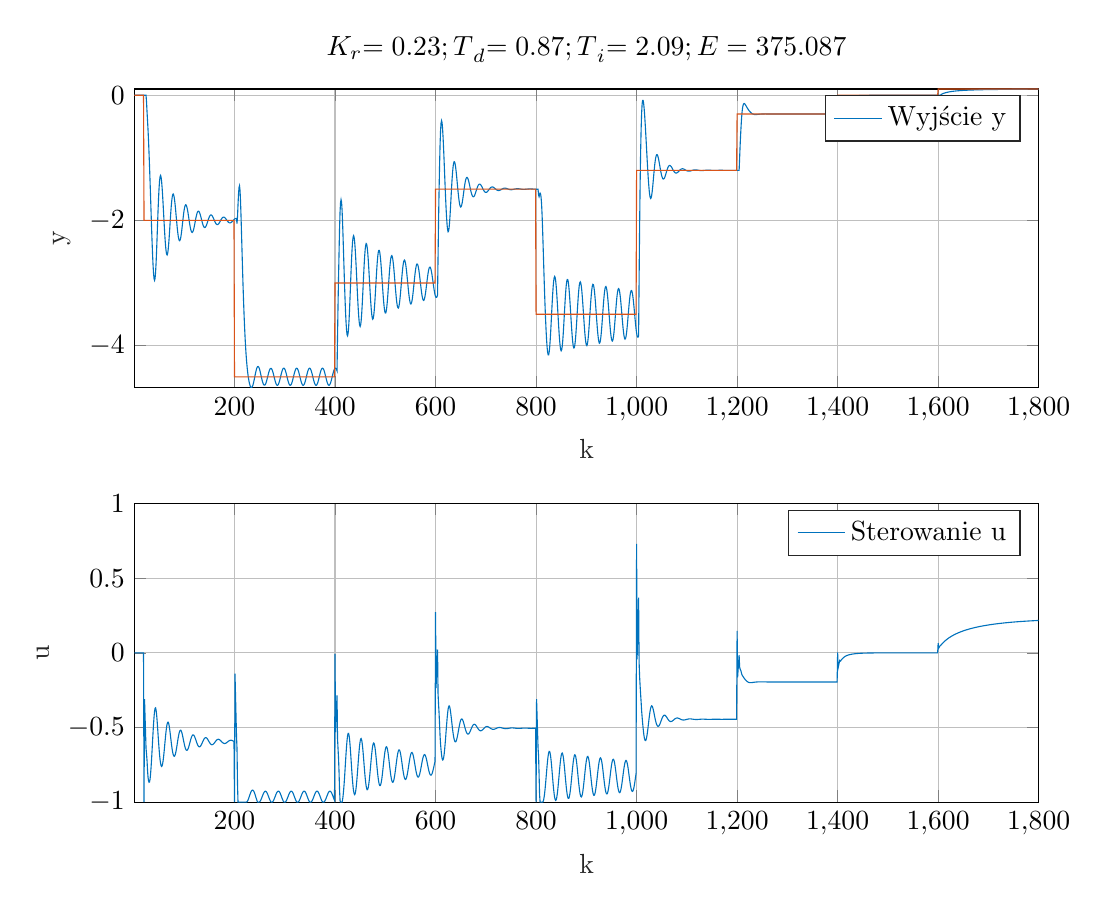
\begin{tikzpicture}

\begin{axis}[%
width=4.521in,
height=1.493in,
at={(0.758in,2.554in)},
scale only axis,
xmin=1,
xmax=1800,
xlabel style={font=\color{white!15!black}},
xlabel={k},
ymin=-4.6706,
ymax=0.1,
ylabel style={font=\color{white!15!black}},
ylabel={y},
axis background/.style={fill=white},
title style={font=\bfseries},
title={$\text{K}_\text{r}\text{=0.23; T}_\text{d}\text{=0.87; T}_\text{i}\text{=2.09; E=375.087}$},
xmajorgrids,
ymajorgrids,
legend style={legend cell align=left, align=left, draw=white!15!black}
]
\addplot [color=mycolor1]
  table[row sep=crcr]{%
1	0\\
2	0\\
3	0\\
4	0\\
5	0\\
6	0\\
7	0\\
8	0\\
9	0\\
10	0\\
11	0\\
12	0\\
13	0\\
14	0\\
15	0\\
16	0\\
17	0\\
18	0\\
19	0\\
20	0\\
21	0\\
22	0\\
23	0\\
24	0\\
25	-0.10916\\
26	-0.26768\\
27	-0.40783\\
28	-0.55718\\
29	-0.73243\\
30	-0.93086\\
31	-1.1447\\
32	-1.3737\\
33	-1.6159\\
34	-1.8637\\
35	-2.1077\\
36	-2.3384\\
37	-2.5461\\
38	-2.7207\\
39	-2.8524\\
40	-2.9335\\
41	-2.9578\\
42	-2.9224\\
43	-2.828\\
44	-2.6798\\
45	-2.4885\\
46	-2.2694\\
47	-2.0409\\
48	-1.8216\\
49	-1.6279\\
50	-1.4718\\
51	-1.3607\\
52	-1.2976\\
53	-1.282\\
54	-1.3106\\
55	-1.3781\\
56	-1.478\\
57	-1.6027\\
58	-1.7442\\
59	-1.8942\\
60	-2.0444\\
61	-2.1868\\
62	-2.3139\\
63	-2.419\\
64	-2.4964\\
65	-2.5418\\
66	-2.5527\\
67	-2.5287\\
68	-2.4714\\
69	-2.3851\\
70	-2.2762\\
71	-2.1531\\
72	-2.0249\\
73	-1.901\\
74	-1.7899\\
75	-1.6984\\
76	-1.6311\\
77	-1.5908\\
78	-1.578\\
79	-1.5917\\
80	-1.6292\\
81	-1.6869\\
82	-1.7604\\
83	-1.8448\\
84	-1.9347\\
85	-2.0249\\
86	-2.1103\\
87	-2.1861\\
88	-2.2484\\
89	-2.2937\\
90	-2.3197\\
91	-2.3251\\
92	-2.3102\\
93	-2.2761\\
94	-2.2257\\
95	-2.1626\\
96	-2.0915\\
97	-2.0174\\
98	-1.9455\\
99	-1.8804\\
100	-1.8259\\
101	-1.7851\\
102	-1.7597\\
103	-1.7504\\
104	-1.7569\\
105	-1.7778\\
106	-1.8112\\
107	-1.8545\\
108	-1.9046\\
109	-1.9583\\
110	-2.0124\\
111	-2.0637\\
112	-2.1092\\
113	-2.1465\\
114	-2.1735\\
115	-2.189\\
116	-2.1923\\
117	-2.1835\\
118	-2.1636\\
119	-2.1342\\
120	-2.0974\\
121	-2.0559\\
122	-2.0126\\
123	-1.9703\\
124	-1.9318\\
125	-1.8992\\
126	-1.8744\\
127	-1.8585\\
128	-1.8522\\
129	-1.8552\\
130	-1.8669\\
131	-1.8862\\
132	-1.9116\\
133	-1.9413\\
134	-1.9733\\
135	-2.0056\\
136	-2.0363\\
137	-2.0637\\
138	-2.0861\\
139	-2.1024\\
140	-2.1118\\
141	-2.114\\
142	-2.109\\
143	-2.0975\\
144	-2.0803\\
145	-2.0588\\
146	-2.0344\\
147	-2.0089\\
148	-1.984\\
149	-1.961\\
150	-1.9415\\
151	-1.9265\\
152	-1.9167\\
153	-1.9124\\
154	-1.9137\\
155	-1.9203\\
156	-1.9315\\
157	-1.9464\\
158	-1.9639\\
159	-1.9829\\
160	-2.0022\\
161	-2.0206\\
162	-2.037\\
163	-2.0505\\
164	-2.0603\\
165	-2.0661\\
166	-2.0676\\
167	-2.0648\\
168	-2.0582\\
169	-2.0482\\
170	-2.0356\\
171	-2.0213\\
172	-2.0062\\
173	-1.9914\\
174	-1.9777\\
175	-1.966\\
176	-1.9569\\
177	-1.9509\\
178	-1.9481\\
179	-1.9487\\
180	-1.9523\\
181	-1.9588\\
182	-1.9675\\
183	-1.9779\\
184	-1.9891\\
185	-2.0006\\
186	-2.0116\\
187	-2.0214\\
188	-2.0295\\
189	-2.0355\\
190	-2.0391\\
191	-2.0401\\
192	-2.0386\\
193	-2.0348\\
194	-2.0289\\
195	-2.0216\\
196	-2.0131\\
197	-2.0042\\
198	-1.9954\\
199	-1.9873\\
200	-1.9803\\
201	-1.9748\\
202	-1.9711\\
203	-1.9693\\
204	-1.9695\\
205	-2.0509\\
206	-1.9428\\
207	-1.7504\\
208	-1.5791\\
209	-1.475\\
210	-1.4472\\
211	-1.5185\\
212	-1.6916\\
213	-1.9337\\
214	-2.2095\\
215	-2.4948\\
216	-2.7741\\
217	-3.0377\\
218	-3.2799\\
219	-3.4981\\
220	-3.6918\\
221	-3.8615\\
222	-4.0087\\
223	-4.1352\\
224	-4.2432\\
225	-4.3348\\
226	-4.4119\\
227	-4.4766\\
228	-4.5306\\
229	-4.5753\\
230	-4.6116\\
231	-4.6395\\
232	-4.6589\\
233	-4.6693\\
234	-4.6706\\
235	-4.6628\\
236	-4.6461\\
237	-4.6214\\
238	-4.59\\
239	-4.5534\\
240	-4.5138\\
241	-4.4733\\
242	-4.4345\\
243	-4.3995\\
244	-4.3704\\
245	-4.349\\
246	-4.3365\\
247	-4.3336\\
248	-4.3406\\
249	-4.357\\
250	-4.3818\\
251	-4.4136\\
252	-4.4493\\
253	-4.4859\\
254	-4.5216\\
255	-4.5548\\
256	-4.5837\\
257	-4.6068\\
258	-4.6231\\
259	-4.6318\\
260	-4.6324\\
261	-4.625\\
262	-4.6101\\
263	-4.5884\\
264	-4.5614\\
265	-4.5306\\
266	-4.4978\\
267	-4.4649\\
268	-4.4341\\
269	-4.4072\\
270	-4.3856\\
271	-4.3709\\
272	-4.3638\\
273	-4.3647\\
274	-4.3737\\
275	-4.3901\\
276	-4.413\\
277	-4.4412\\
278	-4.4729\\
279	-4.506\\
280	-4.5385\\
281	-4.5686\\
282	-4.5948\\
283	-4.6153\\
284	-4.629\\
285	-4.6351\\
286	-4.6331\\
287	-4.6232\\
288	-4.6059\\
289	-4.5821\\
290	-4.5532\\
291	-4.521\\
292	-4.4873\\
293	-4.4543\\
294	-4.4238\\
295	-4.3978\\
296	-4.3778\\
297	-4.365\\
298	-4.3602\\
299	-4.3637\\
300	-4.3752\\
301	-4.3941\\
302	-4.4193\\
303	-4.4494\\
304	-4.4822\\
305	-4.5156\\
306	-4.5478\\
307	-4.577\\
308	-4.6015\\
309	-4.6199\\
310	-4.6312\\
311	-4.6346\\
312	-4.6301\\
313	-4.6177\\
314	-4.5982\\
315	-4.5727\\
316	-4.5426\\
317	-4.5099\\
318	-4.4764\\
319	-4.4441\\
320	-4.4151\\
321	-4.3911\\
322	-4.3735\\
323	-4.3633\\
324	-4.3612\\
325	-4.3674\\
326	-4.3813\\
327	-4.4024\\
328	-4.4292\\
329	-4.4603\\
330	-4.4934\\
331	-4.5266\\
332	-4.558\\
333	-4.5858\\
334	-4.6084\\
335	-4.6247\\
336	-4.6335\\
337	-4.6343\\
338	-4.6272\\
339	-4.6123\\
340	-4.5907\\
341	-4.5635\\
342	-4.5323\\
343	-4.499\\
344	-4.4656\\
345	-4.4341\\
346	-4.4065\\
347	-4.3843\\
348	-4.369\\
349	-4.3614\\
350	-4.362\\
351	-4.3708\\
352	-4.3872\\
353	-4.4103\\
354	-4.4387\\
355	-4.4709\\
356	-4.5043\\
357	-4.5372\\
358	-4.5676\\
359	-4.5941\\
360	-4.6148\\
361	-4.6288\\
362	-4.6351\\
363	-4.6333\\
364	-4.6236\\
365	-4.6064\\
366	-4.5827\\
367	-4.5539\\
368	-4.5218\\
369	-4.4881\\
370	-4.455\\
371	-4.4245\\
372	-4.3983\\
373	-4.3782\\
374	-4.3652\\
375	-4.3602\\
376	-4.3635\\
377	-4.3748\\
378	-4.3936\\
379	-4.4187\\
380	-4.4486\\
381	-4.4814\\
382	-4.5149\\
383	-4.5471\\
384	-4.5763\\
385	-4.601\\
386	-4.6195\\
387	-4.631\\
388	-4.6347\\
389	-4.6303\\
390	-4.6181\\
391	-4.5987\\
392	-4.5733\\
393	-4.5434\\
394	-4.5107\\
395	-4.4771\\
396	-4.4449\\
397	-4.4157\\
398	-4.3916\\
399	-4.3738\\
400	-4.3634\\
401	-4.3612\\
402	-4.3671\\
403	-4.3809\\
404	-4.4018\\
405	-3.8586\\
406	-3.3511\\
407	-2.9167\\
408	-2.5202\\
409	-2.1393\\
410	-1.8674\\
411	-1.717\\
412	-1.6678\\
413	-1.707\\
414	-1.8294\\
415	-2.0233\\
416	-2.2634\\
417	-2.5237\\
418	-2.7859\\
419	-3.0379\\
420	-3.2699\\
421	-3.4721\\
422	-3.6363\\
423	-3.7561\\
424	-3.8263\\
425	-3.8435\\
426	-3.8067\\
427	-3.7178\\
428	-3.582\\
429	-3.4083\\
430	-3.2088\\
431	-2.9983\\
432	-2.7924\\
433	-2.6057\\
434	-2.4503\\
435	-2.3353\\
436	-2.2659\\
437	-2.2439\\
438	-2.2682\\
439	-2.3352\\
440	-2.4393\\
441	-2.5734\\
442	-2.7292\\
443	-2.8979\\
444	-3.0702\\
445	-3.2366\\
446	-3.3882\\
447	-3.5164\\
448	-3.6139\\
449	-3.6747\\
450	-3.6944\\
451	-3.6713\\
452	-3.6058\\
453	-3.5015\\
454	-3.365\\
455	-3.2055\\
456	-3.0343\\
457	-2.8637\\
458	-2.7056\\
459	-2.5705\\
460	-2.4666\\
461	-2.399\\
462	-2.3705\\
463	-2.3809\\
464	-2.428\\
465	-2.5076\\
466	-2.6141\\
467	-2.7409\\
468	-2.8805\\
469	-3.025\\
470	-3.1664\\
471	-3.2968\\
472	-3.409\\
473	-3.4966\\
474	-3.5542\\
475	-3.5781\\
476	-3.5664\\
477	-3.5194\\
478	-3.4396\\
479	-3.3321\\
480	-3.2039\\
481	-3.0639\\
482	-2.9219\\
483	-2.7876\\
484	-2.67\\
485	-2.5762\\
486	-2.5113\\
487	-2.4784\\
488	-2.478\\
489	-2.509\\
490	-2.5684\\
491	-2.652\\
492	-2.7542\\
493	-2.869\\
494	-2.9896\\
495	-3.1094\\
496	-3.2215\\
497	-3.3197\\
498	-3.3984\\
499	-3.4528\\
500	-3.4796\\
501	-3.477\\
502	-3.4448\\
503	-3.3849\\
504	-3.3009\\
505	-3.1985\\
506	-3.0844\\
507	-2.9666\\
508	-2.8529\\
509	-2.7509\\
510	-2.6669\\
511	-2.6057\\
512	-2.5703\\
513	-2.562\\
514	-2.5804\\
515	-2.6234\\
516	-2.6879\\
517	-2.7695\\
518	-2.8632\\
519	-2.9634\\
520	-3.0645\\
521	-3.1606\\
522	-3.2463\\
523	-3.3167\\
524	-3.3677\\
525	-3.3962\\
526	-3.4004\\
527	-3.3799\\
528	-3.3358\\
529	-3.271\\
530	-3.1897\\
531	-3.0972\\
532	-2.9997\\
533	-2.9039\\
534	-2.8159\\
535	-2.7413\\
536	-2.6844\\
537	-2.6483\\
538	-2.6345\\
539	-2.6433\\
540	-2.6732\\
541	-2.7221\\
542	-2.7865\\
543	-2.8623\\
544	-2.9451\\
545	-3.03\\
546	-3.112\\
547	-3.1866\\
548	-3.2493\\
549	-3.2966\\
550	-3.3257\\
551	-3.3347\\
552	-3.3232\\
553	-3.2917\\
554	-3.2423\\
555	-3.1782\\
556	-3.1036\\
557	-3.0234\\
558	-2.9429\\
559	-2.8675\\
560	-2.8017\\
561	-2.7496\\
562	-2.7141\\
563	-2.6969\\
564	-2.6984\\
565	-2.7181\\
566	-2.7544\\
567	-2.8046\\
568	-2.8655\\
569	-2.9334\\
570	-3.0043\\
571	-3.074\\
572	-3.1385\\
573	-3.1941\\
574	-3.2375\\
575	-3.2662\\
576	-3.2785\\
577	-3.2737\\
578	-3.2521\\
579	-3.215\\
580	-3.1649\\
581	-3.1051\\
582	-3.0394\\
583	-2.9722\\
584	-2.9079\\
585	-2.8504\\
586	-2.8033\\
587	-2.7693\\
588	-2.7501\\
589	-2.7465\\
590	-2.7584\\
591	-2.7845\\
592	-2.8231\\
593	-2.8716\\
594	-2.9269\\
595	-2.9858\\
596	-3.0447\\
597	-3.1002\\
598	-3.1491\\
599	-3.1886\\
600	-3.2162\\
601	-3.2306\\
602	-3.2307\\
603	-3.2166\\
604	-3.1894\\
605	-2.5814\\
606	-2.015\\
607	-1.5371\\
608	-1.1314\\
609	-0.79407\\
610	-0.56257\\
611	-0.44143\\
612	-0.40677\\
613	-0.44144\\
614	-0.53462\\
615	-0.67436\\
616	-0.84664\\
617	-1.0392\\
618	-1.2415\\
619	-1.4438\\
620	-1.6364\\
621	-1.8104\\
622	-1.958\\
623	-2.0723\\
624	-2.1478\\
625	-2.1807\\
626	-2.1698\\
627	-2.1162\\
628	-2.0246\\
629	-1.9025\\
630	-1.7602\\
631	-1.6098\\
632	-1.463\\
633	-1.3304\\
634	-1.22\\
635	-1.1372\\
636	-1.0844\\
637	-1.0617\\
638	-1.0675\\
639	-1.0985\\
640	-1.1506\\
641	-1.2191\\
642	-1.299\\
643	-1.3851\\
644	-1.4722\\
645	-1.5556\\
646	-1.6309\\
647	-1.6941\\
648	-1.7423\\
649	-1.7733\\
650	-1.7859\\
651	-1.7801\\
652	-1.7571\\
653	-1.7191\\
654	-1.6695\\
655	-1.6121\\
656	-1.5512\\
657	-1.4911\\
658	-1.4358\\
659	-1.3885\\
660	-1.3517\\
661	-1.3267\\
662	-1.3143\\
663	-1.3142\\
664	-1.3253\\
665	-1.3462\\
666	-1.3749\\
667	-1.4091\\
668	-1.4465\\
669	-1.4847\\
670	-1.5214\\
671	-1.5545\\
672	-1.5823\\
673	-1.6035\\
674	-1.6171\\
675	-1.6226\\
676	-1.6203\\
677	-1.6107\\
678	-1.5948\\
679	-1.574\\
680	-1.5498\\
681	-1.5241\\
682	-1.4986\\
683	-1.4749\\
684	-1.4543\\
685	-1.438\\
686	-1.4266\\
687	-1.4205\\
688	-1.4197\\
689	-1.4239\\
690	-1.4324\\
691	-1.4445\\
692	-1.4591\\
693	-1.4753\\
694	-1.4919\\
695	-1.5079\\
696	-1.5225\\
697	-1.5347\\
698	-1.5441\\
699	-1.5502\\
700	-1.5528\\
701	-1.552\\
702	-1.548\\
703	-1.5414\\
704	-1.5326\\
705	-1.5223\\
706	-1.5114\\
707	-1.5004\\
708	-1.4901\\
709	-1.4812\\
710	-1.4739\\
711	-1.4688\\
712	-1.4659\\
713	-1.4653\\
714	-1.4669\\
715	-1.4704\\
716	-1.4755\\
717	-1.4817\\
718	-1.4887\\
719	-1.4959\\
720	-1.5028\\
721	-1.5092\\
722	-1.5146\\
723	-1.5187\\
724	-1.5215\\
725	-1.5227\\
726	-1.5225\\
727	-1.5209\\
728	-1.5181\\
729	-1.5144\\
730	-1.51\\
731	-1.5053\\
732	-1.5006\\
733	-1.4961\\
734	-1.4922\\
735	-1.489\\
736	-1.4867\\
737	-1.4854\\
738	-1.485\\
739	-1.4856\\
740	-1.4871\\
741	-1.4892\\
742	-1.4918\\
743	-1.4948\\
744	-1.4979\\
745	-1.501\\
746	-1.5037\\
747	-1.5061\\
748	-1.5079\\
749	-1.5092\\
750	-1.5098\\
751	-1.5097\\
752	-1.5091\\
753	-1.5079\\
754	-1.5064\\
755	-1.5045\\
756	-1.5025\\
757	-1.5004\\
758	-1.4985\\
759	-1.4968\\
760	-1.4954\\
761	-1.4944\\
762	-1.4937\\
763	-1.4935\\
764	-1.4938\\
765	-1.4943\\
766	-1.4952\\
767	-1.4964\\
768	-1.4976\\
769	-1.499\\
770	-1.5003\\
771	-1.5015\\
772	-1.5026\\
773	-1.5034\\
774	-1.5039\\
775	-1.5042\\
776	-1.5042\\
777	-1.504\\
778	-1.5035\\
779	-1.5028\\
780	-1.502\\
781	-1.5011\\
782	-1.5003\\
783	-1.4994\\
784	-1.4987\\
785	-1.4981\\
786	-1.4976\\
787	-1.4973\\
788	-1.4972\\
789	-1.4973\\
790	-1.4975\\
791	-1.4979\\
792	-1.4984\\
793	-1.4989\\
794	-1.4995\\
795	-1.5001\\
796	-1.5006\\
797	-1.5011\\
798	-1.5014\\
799	-1.5017\\
800	-1.5018\\
801	-1.5018\\
802	-1.5017\\
803	-1.5015\\
804	-1.5012\\
805	-1.5939\\
806	-1.6209\\
807	-1.5898\\
808	-1.5641\\
809	-1.5769\\
810	-1.6327\\
811	-1.7407\\
812	-1.9124\\
813	-2.1392\\
814	-2.3964\\
815	-2.662\\
816	-2.9215\\
817	-3.1662\\
818	-3.3908\\
819	-3.5924\\
820	-3.768\\
821	-3.9143\\
822	-4.0282\\
823	-4.1066\\
824	-4.1473\\
825	-4.1486\\
826	-4.1107\\
827	-4.0357\\
828	-3.9278\\
829	-3.7936\\
830	-3.6417\\
831	-3.4821\\
832	-3.3257\\
833	-3.1828\\
834	-3.0623\\
835	-2.9715\\
836	-2.915\\
837	-2.8951\\
838	-2.9118\\
839	-2.9631\\
840	-3.0451\\
841	-3.1524\\
842	-3.2786\\
843	-3.4164\\
844	-3.5582\\
845	-3.696\\
846	-3.8224\\
847	-3.93\\
848	-4.0126\\
849	-4.065\\
850	-4.0836\\
851	-4.0668\\
852	-4.0147\\
853	-3.9302\\
854	-3.8182\\
855	-3.6859\\
856	-3.5421\\
857	-3.3966\\
858	-3.2591\\
859	-3.1387\\
860	-3.0427\\
861	-2.9767\\
862	-2.9438\\
863	-2.9451\\
864	-2.9793\\
865	-3.0438\\
866	-3.134\\
867	-3.2445\\
868	-3.3687\\
869	-3.4996\\
870	-3.6299\\
871	-3.7523\\
872	-3.86\\
873	-3.9467\\
874	-4.0071\\
875	-4.0374\\
876	-4.0352\\
877	-4\\
878	-3.9337\\
879	-3.8399\\
880	-3.7245\\
881	-3.5951\\
882	-3.4603\\
883	-3.3291\\
884	-3.2103\\
885	-3.1112\\
886	-3.0379\\
887	-2.9941\\
888	-2.9817\\
889	-3.0006\\
890	-3.0488\\
891	-3.1228\\
892	-3.218\\
893	-3.3286\\
894	-3.4482\\
895	-3.5702\\
896	-3.6876\\
897	-3.794\\
898	-3.883\\
899	-3.9496\\
900	-3.9895\\
901	-4.0001\\
902	-3.9801\\
903	-3.9303\\
904	-3.8536\\
905	-3.7546\\
906	-3.6395\\
907	-3.5161\\
908	-3.3926\\
909	-3.277\\
910	-3.1769\\
911	-3.0983\\
912	-3.0456\\
913	-3.0214\\
914	-3.0264\\
915	-3.0596\\
916	-3.1184\\
917	-3.1988\\
918	-3.2959\\
919	-3.4041\\
920	-3.5171\\
921	-3.6285\\
922	-3.7322\\
923	-3.8222\\
924	-3.8932\\
925	-3.941\\
926	-3.9623\\
927	-3.9556\\
928	-3.921\\
929	-3.8601\\
930	-3.7767\\
931	-3.6759\\
932	-3.5643\\
933	-3.4493\\
934	-3.3384\\
935	-3.239\\
936	-3.157\\
937	-3.0974\\
938	-3.0633\\
939	-3.0562\\
940	-3.0757\\
941	-3.1201\\
942	-3.1864\\
943	-3.2703\\
944	-3.3669\\
945	-3.4705\\
946	-3.5752\\
947	-3.6752\\
948	-3.7646\\
949	-3.8385\\
950	-3.8923\\
951	-3.9227\\
952	-3.9276\\
953	-3.9064\\
954	-3.8601\\
955	-3.7914\\
956	-3.7044\\
957	-3.6048\\
958	-3.4991\\
959	-3.3942\\
960	-3.297\\
961	-3.2135\\
962	-3.1488\\
963	-3.1066\\
964	-3.0889\\
965	-3.0962\\
966	-3.1274\\
967	-3.1804\\
968	-3.2515\\
969	-3.3365\\
970	-3.4304\\
971	-3.5277\\
972	-3.623\\
973	-3.7107\\
974	-3.786\\
975	-3.8443\\
976	-3.882\\
977	-3.8968\\
978	-3.8876\\
979	-3.8545\\
980	-3.7995\\
981	-3.7258\\
982	-3.6382\\
983	-3.5422\\
984	-3.4442\\
985	-3.3505\\
986	-3.267\\
987	-3.1991\\
988	-3.1505\\
989	-3.1238\\
990	-3.1203\\
991	-3.1396\\
992	-3.18\\
993	-3.2389\\
994	-3.3126\\
995	-3.3966\\
996	-3.486\\
997	-3.5758\\
998	-3.6608\\
999	-3.7361\\
1000	-3.7974\\
1001	-3.841\\
1002	-3.8641\\
1003	-3.8652\\
1004	-3.844\\
1005	-2.9557\\
1006	-2.1213\\
1007	-1.4429\\
1008	-0.92373\\
1009	-0.55296\\
1010	-0.29126\\
1011	-0.14385\\
1012	-0.081951\\
1013	-0.082166\\
1014	-0.12771\\
1015	-0.20826\\
1016	-0.31501\\
1017	-0.44031\\
1018	-0.57855\\
1019	-0.72509\\
1020	-0.8753\\
1021	-1.0244\\
1022	-1.1675\\
1023	-1.2998\\
1024	-1.4164\\
1025	-1.513\\
1026	-1.5857\\
1027	-1.6318\\
1028	-1.6496\\
1029	-1.6392\\
1030	-1.6026\\
1031	-1.5433\\
1032	-1.4667\\
1033	-1.3792\\
1034	-1.2878\\
1035	-1.1992\\
1036	-1.1191\\
1037	-1.0522\\
1038	-1.0012\\
1039	-0.96755\\
1040	-0.95142\\
1041	-0.95179\\
1042	-0.96679\\
1043	-0.99401\\
1044	-1.0307\\
1045	-1.0738\\
1046	-1.1203\\
1047	-1.1675\\
1048	-1.2125\\
1049	-1.253\\
1050	-1.2871\\
1051	-1.3132\\
1052	-1.3305\\
1053	-1.3385\\
1054	-1.3374\\
1055	-1.328\\
1056	-1.3115\\
1057	-1.2895\\
1058	-1.2638\\
1059	-1.2364\\
1060	-1.2091\\
1061	-1.1837\\
1062	-1.1616\\
1063	-1.1439\\
1064	-1.1311\\
1065	-1.1238\\
1066	-1.1217\\
1067	-1.1245\\
1068	-1.1316\\
1069	-1.1422\\
1070	-1.1553\\
1071	-1.1699\\
1072	-1.185\\
1073	-1.1998\\
1074	-1.2132\\
1075	-1.2248\\
1076	-1.2338\\
1077	-1.2401\\
1078	-1.2434\\
1079	-1.2438\\
1080	-1.2414\\
1081	-1.2368\\
1082	-1.2303\\
1083	-1.2226\\
1084	-1.2141\\
1085	-1.2055\\
1086	-1.1973\\
1087	-1.19\\
1088	-1.184\\
1089	-1.1794\\
1090	-1.1765\\
1091	-1.1753\\
1092	-1.1757\\
1093	-1.1775\\
1094	-1.1805\\
1095	-1.1845\\
1096	-1.189\\
1097	-1.1938\\
1098	-1.1985\\
1099	-1.203\\
1100	-1.2068\\
1101	-1.2099\\
1102	-1.2122\\
1103	-1.2135\\
1104	-1.2139\\
1105	-1.2134\\
1106	-1.2121\\
1107	-1.2103\\
1108	-1.2079\\
1109	-1.2053\\
1110	-1.2026\\
1111	-1.1999\\
1112	-1.1975\\
1113	-1.1955\\
1114	-1.1939\\
1115	-1.1928\\
1116	-1.1923\\
1117	-1.1922\\
1118	-1.1927\\
1119	-1.1935\\
1120	-1.1947\\
1121	-1.1961\\
1122	-1.1976\\
1123	-1.1991\\
1124	-1.2005\\
1125	-1.2018\\
1126	-1.2029\\
1127	-1.2037\\
1128	-1.2042\\
1129	-1.2044\\
1130	-1.2043\\
1131	-1.204\\
1132	-1.2034\\
1133	-1.2027\\
1134	-1.2019\\
1135	-1.2011\\
1136	-1.2002\\
1137	-1.1994\\
1138	-1.1988\\
1139	-1.1982\\
1140	-1.1978\\
1141	-1.1976\\
1142	-1.1975\\
1143	-1.1976\\
1144	-1.1979\\
1145	-1.1982\\
1146	-1.1986\\
1147	-1.1991\\
1148	-1.1996\\
1149	-1.2\\
1150	-1.2005\\
1151	-1.2008\\
1152	-1.2011\\
1153	-1.2013\\
1154	-1.2014\\
1155	-1.2014\\
1156	-1.2013\\
1157	-1.2011\\
1158	-1.2009\\
1159	-1.2007\\
1160	-1.2004\\
1161	-1.2002\\
1162	-1.1999\\
1163	-1.1997\\
1164	-1.1995\\
1165	-1.1993\\
1166	-1.1993\\
1167	-1.1992\\
1168	-1.1992\\
1169	-1.1993\\
1170	-1.1994\\
1171	-1.1995\\
1172	-1.1997\\
1173	-1.1998\\
1174	-1.2\\
1175	-1.2001\\
1176	-1.2002\\
1177	-1.2003\\
1178	-1.2004\\
1179	-1.2004\\
1180	-1.2004\\
1181	-1.2004\\
1182	-1.2004\\
1183	-1.2003\\
1184	-1.2002\\
1185	-1.2002\\
1186	-1.2001\\
1187	-1.2\\
1188	-1.1999\\
1189	-1.1999\\
1190	-1.1998\\
1191	-1.1998\\
1192	-1.1998\\
1193	-1.1998\\
1194	-1.1998\\
1195	-1.1998\\
1196	-1.1998\\
1197	-1.1999\\
1198	-1.1999\\
1199	-1.2\\
1200	-1.2\\
1201	-1.2001\\
1202	-1.2001\\
1203	-1.2001\\
1204	-1.2001\\
1205	-1.0067\\
1206	-0.80456\\
1207	-0.63167\\
1208	-0.48242\\
1209	-0.35423\\
1210	-0.25777\\
1211	-0.19482\\
1212	-0.15721\\
1213	-0.13794\\
1214	-0.13238\\
1215	-0.13643\\
1216	-0.14619\\
1217	-0.15888\\
1218	-0.17284\\
1219	-0.18705\\
1220	-0.2009\\
1221	-0.21404\\
1222	-0.22639\\
1223	-0.23791\\
1224	-0.24861\\
1225	-0.25846\\
1226	-0.26746\\
1227	-0.2756\\
1228	-0.28282\\
1229	-0.28912\\
1230	-0.29449\\
1231	-0.29892\\
1232	-0.30246\\
1233	-0.30516\\
1234	-0.30708\\
1235	-0.30832\\
1236	-0.30897\\
1237	-0.30913\\
1238	-0.3089\\
1239	-0.30838\\
1240	-0.30764\\
1241	-0.30678\\
1242	-0.30585\\
1243	-0.30491\\
1244	-0.30399\\
1245	-0.30313\\
1246	-0.30235\\
1247	-0.30167\\
1248	-0.30107\\
1249	-0.30058\\
1250	-0.30018\\
1251	-0.29986\\
1252	-0.29962\\
1253	-0.29946\\
1254	-0.29935\\
1255	-0.29929\\
1256	-0.29927\\
1257	-0.29929\\
1258	-0.29932\\
1259	-0.29938\\
1260	-0.29944\\
1261	-0.29951\\
1262	-0.29959\\
1263	-0.29966\\
1264	-0.29973\\
1265	-0.29979\\
1266	-0.29984\\
1267	-0.29989\\
1268	-0.29994\\
1269	-0.29997\\
1270	-0.3\\
1271	-0.30002\\
1272	-0.30004\\
1273	-0.30005\\
1274	-0.30005\\
1275	-0.30006\\
1276	-0.30006\\
1277	-0.30005\\
1278	-0.30005\\
1279	-0.30005\\
1280	-0.30004\\
1281	-0.30004\\
1282	-0.30003\\
1283	-0.30002\\
1284	-0.30002\\
1285	-0.30001\\
1286	-0.30001\\
1287	-0.30001\\
1288	-0.3\\
1289	-0.3\\
1290	-0.3\\
1291	-0.3\\
1292	-0.3\\
1293	-0.3\\
1294	-0.3\\
1295	-0.3\\
1296	-0.3\\
1297	-0.3\\
1298	-0.3\\
1299	-0.3\\
1300	-0.3\\
1301	-0.3\\
1302	-0.3\\
1303	-0.3\\
1304	-0.3\\
1305	-0.3\\
1306	-0.3\\
1307	-0.3\\
1308	-0.3\\
1309	-0.3\\
1310	-0.3\\
1311	-0.3\\
1312	-0.3\\
1313	-0.3\\
1314	-0.3\\
1315	-0.3\\
1316	-0.3\\
1317	-0.3\\
1318	-0.3\\
1319	-0.3\\
1320	-0.3\\
1321	-0.3\\
1322	-0.3\\
1323	-0.3\\
1324	-0.3\\
1325	-0.3\\
1326	-0.3\\
1327	-0.3\\
1328	-0.3\\
1329	-0.3\\
1330	-0.3\\
1331	-0.3\\
1332	-0.3\\
1333	-0.3\\
1334	-0.3\\
1335	-0.3\\
1336	-0.3\\
1337	-0.3\\
1338	-0.3\\
1339	-0.3\\
1340	-0.3\\
1341	-0.3\\
1342	-0.3\\
1343	-0.3\\
1344	-0.3\\
1345	-0.3\\
1346	-0.3\\
1347	-0.3\\
1348	-0.3\\
1349	-0.3\\
1350	-0.3\\
1351	-0.3\\
1352	-0.3\\
1353	-0.3\\
1354	-0.3\\
1355	-0.3\\
1356	-0.3\\
1357	-0.3\\
1358	-0.3\\
1359	-0.3\\
1360	-0.3\\
1361	-0.3\\
1362	-0.3\\
1363	-0.3\\
1364	-0.3\\
1365	-0.3\\
1366	-0.3\\
1367	-0.3\\
1368	-0.3\\
1369	-0.3\\
1370	-0.3\\
1371	-0.3\\
1372	-0.3\\
1373	-0.3\\
1374	-0.3\\
1375	-0.3\\
1376	-0.3\\
1377	-0.3\\
1378	-0.3\\
1379	-0.3\\
1380	-0.3\\
1381	-0.3\\
1382	-0.3\\
1383	-0.3\\
1384	-0.3\\
1385	-0.3\\
1386	-0.3\\
1387	-0.3\\
1388	-0.3\\
1389	-0.3\\
1390	-0.3\\
1391	-0.3\\
1392	-0.3\\
1393	-0.3\\
1394	-0.3\\
1395	-0.3\\
1396	-0.3\\
1397	-0.3\\
1398	-0.3\\
1399	-0.3\\
1400	-0.3\\
1401	-0.3\\
1402	-0.3\\
1403	-0.3\\
1404	-0.3\\
1405	-0.26838\\
1406	-0.22873\\
1407	-0.19444\\
1408	-0.16398\\
1409	-0.1364\\
1410	-0.11314\\
1411	-0.094989\\
1412	-0.08092\\
1413	-0.069815\\
1414	-0.060998\\
1415	-0.053927\\
1416	-0.048097\\
1417	-0.043129\\
1418	-0.038805\\
1419	-0.034994\\
1420	-0.031611\\
1421	-0.028597\\
1422	-0.025917\\
1423	-0.023539\\
1424	-0.021433\\
1425	-0.01957\\
1426	-0.017919\\
1427	-0.016454\\
1428	-0.015147\\
1429	-0.013978\\
1430	-0.012925\\
1431	-0.011973\\
1432	-0.011107\\
1433	-0.010318\\
1434	-0.0095946\\
1435	-0.0089308\\
1436	-0.0083199\\
1437	-0.0077566\\
1438	-0.0072363\\
1439	-0.006755\\
1440	-0.0063092\\
1441	-0.0058958\\
1442	-0.0055121\\
1443	-0.0051555\\
1444	-0.0048238\\
1445	-0.004515\\
1446	-0.0042273\\
1447	-0.0039591\\
1448	-0.0037088\\
1449	-0.0034752\\
1450	-0.003257\\
1451	-0.003053\\
1452	-0.0028624\\
1453	-0.0026841\\
1454	-0.0025173\\
1455	-0.0023612\\
1456	-0.0022151\\
1457	-0.0020782\\
1458	-0.0019501\\
1459	-0.00183\\
1460	-0.0017175\\
1461	-0.0016121\\
1462	-0.0015132\\
1463	-0.0014205\\
1464	-0.0013336\\
1465	-0.0012521\\
1466	-0.0011757\\
1467	-0.001104\\
1468	-0.0010367\\
1469	-0.00097357\\
1470	-0.00091433\\
1471	-0.00085873\\
1472	-0.00080654\\
1473	-0.00075756\\
1474	-0.00071158\\
1475	-0.00066841\\
1476	-0.00062789\\
1477	-0.00058983\\
1478	-0.0005541\\
1479	-0.00052055\\
1480	-0.00048904\\
1481	-0.00045945\\
1482	-0.00043166\\
1483	-0.00040556\\
1484	-0.00038105\\
1485	-0.00035802\\
1486	-0.00033639\\
1487	-0.00031607\\
1488	-0.00029699\\
1489	-0.00027906\\
1490	-0.00026222\\
1491	-0.00024639\\
1492	-0.00023153\\
1493	-0.00021756\\
1494	-0.00020444\\
1495	-0.00019211\\
1496	-0.00018052\\
1497	-0.00016964\\
1498	-0.00015941\\
1499	-0.00014981\\
1500	-0.00014078\\
1501	-0.00013229\\
1502	-0.00012432\\
1503	-0.00011683\\
1504	-0.00010979\\
1505	-0.00010318\\
1506	-9.6964e-05\\
1507	-9.1123e-05\\
1508	-8.5635e-05\\
1509	-8.0478e-05\\
1510	-7.5632e-05\\
1511	-7.1077e-05\\
1512	-6.6797e-05\\
1513	-6.2775e-05\\
1514	-5.8996e-05\\
1515	-5.5444e-05\\
1516	-5.2106e-05\\
1517	-4.8969e-05\\
1518	-4.6021e-05\\
1519	-4.3251e-05\\
1520	-4.0648e-05\\
1521	-3.8201e-05\\
1522	-3.5902e-05\\
1523	-3.3741e-05\\
1524	-3.171e-05\\
1525	-2.9801e-05\\
1526	-2.8008e-05\\
1527	-2.6322e-05\\
1528	-2.4738e-05\\
1529	-2.3249e-05\\
1530	-2.185e-05\\
1531	-2.0535e-05\\
1532	-1.9299e-05\\
1533	-1.8138e-05\\
1534	-1.7047e-05\\
1535	-1.6021e-05\\
1536	-1.5057e-05\\
1537	-1.4151e-05\\
1538	-1.3299e-05\\
1539	-1.2499e-05\\
1540	-1.1747e-05\\
1541	-1.104e-05\\
1542	-1.0376e-05\\
1543	-9.7514e-06\\
1544	-9.1646e-06\\
1545	-8.6132e-06\\
1546	-8.0949e-06\\
1547	-7.6079e-06\\
1548	-7.1501e-06\\
1549	-6.7199e-06\\
1550	-6.3155e-06\\
1551	-5.9355e-06\\
1552	-5.5784e-06\\
1553	-5.2428e-06\\
1554	-4.9273e-06\\
1555	-4.6309e-06\\
1556	-4.3522e-06\\
1557	-4.0904e-06\\
1558	-3.8443e-06\\
1559	-3.613e-06\\
1560	-3.3956e-06\\
1561	-3.1913e-06\\
1562	-2.9993e-06\\
1563	-2.8188e-06\\
1564	-2.6492e-06\\
1565	-2.4898e-06\\
1566	-2.34e-06\\
1567	-2.1992e-06\\
1568	-2.0669e-06\\
1569	-1.9426e-06\\
1570	-1.8257e-06\\
1571	-1.7158e-06\\
1572	-1.6126e-06\\
1573	-1.5156e-06\\
1574	-1.4244e-06\\
1575	-1.3387e-06\\
1576	-1.2582e-06\\
1577	-1.1825e-06\\
1578	-1.1113e-06\\
1579	-1.0445e-06\\
1580	-9.8161e-07\\
1581	-9.2256e-07\\
1582	-8.6705e-07\\
1583	-8.1488e-07\\
1584	-7.6586e-07\\
1585	-7.1978e-07\\
1586	-6.7647e-07\\
1587	-6.3577e-07\\
1588	-5.9752e-07\\
1589	-5.6157e-07\\
1590	-5.2779e-07\\
1591	-4.9603e-07\\
1592	-4.6619e-07\\
1593	-4.3814e-07\\
1594	-4.1178e-07\\
1595	-3.87e-07\\
1596	-3.6372e-07\\
1597	-3.4184e-07\\
1598	-3.2127e-07\\
1599	-3.0194e-07\\
1600	-2.8378e-07\\
1601	-2.667e-07\\
1602	-2.5066e-07\\
1603	-2.3558e-07\\
1604	-2.214e-07\\
1605	0.0038545\\
1606	0.010289\\
1607	0.015376\\
1608	0.019686\\
1609	0.02356\\
1610	0.027078\\
1611	0.030176\\
1612	0.032934\\
1613	0.03549\\
1614	0.037901\\
1615	0.040185\\
1616	0.042352\\
1617	0.044411\\
1618	0.046366\\
1619	0.048217\\
1620	0.049967\\
1621	0.051618\\
1622	0.053178\\
1623	0.054651\\
1624	0.056044\\
1625	0.057363\\
1626	0.058613\\
1627	0.059801\\
1628	0.06093\\
1629	0.062006\\
1630	0.063032\\
1631	0.064011\\
1632	0.064947\\
1633	0.065843\\
1634	0.0667\\
1635	0.067523\\
1636	0.068311\\
1637	0.069069\\
1638	0.069797\\
1639	0.070497\\
1640	0.071172\\
1641	0.071821\\
1642	0.072447\\
1643	0.073051\\
1644	0.073634\\
1645	0.074197\\
1646	0.074741\\
1647	0.075267\\
1648	0.075776\\
1649	0.076269\\
1650	0.076746\\
1651	0.077208\\
1652	0.077656\\
1653	0.078091\\
1654	0.078513\\
1655	0.078922\\
1656	0.07932\\
1657	0.079706\\
1658	0.080082\\
1659	0.080447\\
1660	0.080802\\
1661	0.081147\\
1662	0.081484\\
1663	0.081811\\
1664	0.08213\\
1665	0.08244\\
1666	0.082743\\
1667	0.083038\\
1668	0.083326\\
1669	0.083607\\
1670	0.083881\\
1671	0.084148\\
1672	0.084409\\
1673	0.084663\\
1674	0.084912\\
1675	0.085155\\
1676	0.085393\\
1677	0.085625\\
1678	0.085852\\
1679	0.086074\\
1680	0.086291\\
1681	0.086503\\
1682	0.086711\\
1683	0.086914\\
1684	0.087113\\
1685	0.087308\\
1686	0.087498\\
1687	0.087685\\
1688	0.087868\\
1689	0.088047\\
1690	0.088223\\
1691	0.088395\\
1692	0.088564\\
1693	0.088729\\
1694	0.088891\\
1695	0.08905\\
1696	0.089206\\
1697	0.089359\\
1698	0.089509\\
1699	0.089656\\
1700	0.089801\\
1701	0.089943\\
1702	0.090082\\
1703	0.090218\\
1704	0.090353\\
1705	0.090484\\
1706	0.090614\\
1707	0.090741\\
1708	0.090866\\
1709	0.090989\\
1710	0.091109\\
1711	0.091228\\
1712	0.091344\\
1713	0.091458\\
1714	0.091571\\
1715	0.091682\\
1716	0.09179\\
1717	0.091897\\
1718	0.092002\\
1719	0.092106\\
1720	0.092207\\
1721	0.092307\\
1722	0.092406\\
1723	0.092503\\
1724	0.092598\\
1725	0.092692\\
1726	0.092784\\
1727	0.092875\\
1728	0.092964\\
1729	0.093052\\
1730	0.093139\\
1731	0.093224\\
1732	0.093308\\
1733	0.093391\\
1734	0.093472\\
1735	0.093552\\
1736	0.093631\\
1737	0.093709\\
1738	0.093786\\
1739	0.093861\\
1740	0.093935\\
1741	0.094009\\
1742	0.094081\\
1743	0.094152\\
1744	0.094222\\
1745	0.094291\\
1746	0.094359\\
1747	0.094426\\
1748	0.094492\\
1749	0.094558\\
1750	0.094622\\
1751	0.094685\\
1752	0.094748\\
1753	0.094809\\
1754	0.09487\\
1755	0.09493\\
1756	0.094989\\
1757	0.095047\\
1758	0.095105\\
1759	0.095161\\
1760	0.095217\\
1761	0.095272\\
1762	0.095327\\
1763	0.09538\\
1764	0.095433\\
1765	0.095485\\
1766	0.095537\\
1767	0.095588\\
1768	0.095638\\
1769	0.095687\\
1770	0.095736\\
1771	0.095784\\
1772	0.095832\\
1773	0.095879\\
1774	0.095925\\
1775	0.095971\\
1776	0.096016\\
1777	0.09606\\
1778	0.096104\\
1779	0.096148\\
1780	0.096191\\
1781	0.096233\\
1782	0.096275\\
1783	0.096316\\
1784	0.096357\\
1785	0.096397\\
1786	0.096436\\
1787	0.096476\\
1788	0.096514\\
1789	0.096553\\
1790	0.09659\\
1791	0.096628\\
1792	0.096664\\
1793	0.096701\\
1794	0.096737\\
1795	0.096772\\
1796	0.096807\\
1797	0.096842\\
1798	0.096876\\
1799	0.09691\\
1800	0.096943\\
};
\addlegendentry{Wyjście y}

\addplot [color=mycolor2, forget plot]
  table[row sep=crcr]{%
1	0\\
2	0\\
3	0\\
4	0\\
5	0\\
6	0\\
7	0\\
8	0\\
9	0\\
10	0\\
11	0\\
12	0\\
13	0\\
14	0\\
15	0\\
16	0\\
17	0\\
18	0\\
19	0\\
20	-2\\
21	-2\\
22	-2\\
23	-2\\
24	-2\\
25	-2\\
26	-2\\
27	-2\\
28	-2\\
29	-2\\
30	-2\\
31	-2\\
32	-2\\
33	-2\\
34	-2\\
35	-2\\
36	-2\\
37	-2\\
38	-2\\
39	-2\\
40	-2\\
41	-2\\
42	-2\\
43	-2\\
44	-2\\
45	-2\\
46	-2\\
47	-2\\
48	-2\\
49	-2\\
50	-2\\
51	-2\\
52	-2\\
53	-2\\
54	-2\\
55	-2\\
56	-2\\
57	-2\\
58	-2\\
59	-2\\
60	-2\\
61	-2\\
62	-2\\
63	-2\\
64	-2\\
65	-2\\
66	-2\\
67	-2\\
68	-2\\
69	-2\\
70	-2\\
71	-2\\
72	-2\\
73	-2\\
74	-2\\
75	-2\\
76	-2\\
77	-2\\
78	-2\\
79	-2\\
80	-2\\
81	-2\\
82	-2\\
83	-2\\
84	-2\\
85	-2\\
86	-2\\
87	-2\\
88	-2\\
89	-2\\
90	-2\\
91	-2\\
92	-2\\
93	-2\\
94	-2\\
95	-2\\
96	-2\\
97	-2\\
98	-2\\
99	-2\\
100	-2\\
101	-2\\
102	-2\\
103	-2\\
104	-2\\
105	-2\\
106	-2\\
107	-2\\
108	-2\\
109	-2\\
110	-2\\
111	-2\\
112	-2\\
113	-2\\
114	-2\\
115	-2\\
116	-2\\
117	-2\\
118	-2\\
119	-2\\
120	-2\\
121	-2\\
122	-2\\
123	-2\\
124	-2\\
125	-2\\
126	-2\\
127	-2\\
128	-2\\
129	-2\\
130	-2\\
131	-2\\
132	-2\\
133	-2\\
134	-2\\
135	-2\\
136	-2\\
137	-2\\
138	-2\\
139	-2\\
140	-2\\
141	-2\\
142	-2\\
143	-2\\
144	-2\\
145	-2\\
146	-2\\
147	-2\\
148	-2\\
149	-2\\
150	-2\\
151	-2\\
152	-2\\
153	-2\\
154	-2\\
155	-2\\
156	-2\\
157	-2\\
158	-2\\
159	-2\\
160	-2\\
161	-2\\
162	-2\\
163	-2\\
164	-2\\
165	-2\\
166	-2\\
167	-2\\
168	-2\\
169	-2\\
170	-2\\
171	-2\\
172	-2\\
173	-2\\
174	-2\\
175	-2\\
176	-2\\
177	-2\\
178	-2\\
179	-2\\
180	-2\\
181	-2\\
182	-2\\
183	-2\\
184	-2\\
185	-2\\
186	-2\\
187	-2\\
188	-2\\
189	-2\\
190	-2\\
191	-2\\
192	-2\\
193	-2\\
194	-2\\
195	-2\\
196	-2\\
197	-2\\
198	-2\\
199	-2\\
200	-4.5\\
201	-4.5\\
202	-4.5\\
203	-4.5\\
204	-4.5\\
205	-4.5\\
206	-4.5\\
207	-4.5\\
208	-4.5\\
209	-4.5\\
210	-4.5\\
211	-4.5\\
212	-4.5\\
213	-4.5\\
214	-4.5\\
215	-4.5\\
216	-4.5\\
217	-4.5\\
218	-4.5\\
219	-4.5\\
220	-4.5\\
221	-4.5\\
222	-4.5\\
223	-4.5\\
224	-4.5\\
225	-4.5\\
226	-4.5\\
227	-4.5\\
228	-4.5\\
229	-4.5\\
230	-4.5\\
231	-4.5\\
232	-4.5\\
233	-4.5\\
234	-4.5\\
235	-4.5\\
236	-4.5\\
237	-4.5\\
238	-4.5\\
239	-4.5\\
240	-4.5\\
241	-4.5\\
242	-4.5\\
243	-4.5\\
244	-4.5\\
245	-4.5\\
246	-4.5\\
247	-4.5\\
248	-4.5\\
249	-4.5\\
250	-4.5\\
251	-4.5\\
252	-4.5\\
253	-4.5\\
254	-4.5\\
255	-4.5\\
256	-4.5\\
257	-4.5\\
258	-4.5\\
259	-4.5\\
260	-4.5\\
261	-4.5\\
262	-4.5\\
263	-4.5\\
264	-4.5\\
265	-4.5\\
266	-4.5\\
267	-4.5\\
268	-4.5\\
269	-4.5\\
270	-4.5\\
271	-4.5\\
272	-4.5\\
273	-4.5\\
274	-4.5\\
275	-4.5\\
276	-4.5\\
277	-4.5\\
278	-4.5\\
279	-4.5\\
280	-4.5\\
281	-4.5\\
282	-4.5\\
283	-4.5\\
284	-4.5\\
285	-4.5\\
286	-4.5\\
287	-4.5\\
288	-4.5\\
289	-4.5\\
290	-4.5\\
291	-4.5\\
292	-4.5\\
293	-4.5\\
294	-4.5\\
295	-4.5\\
296	-4.5\\
297	-4.5\\
298	-4.5\\
299	-4.5\\
300	-4.5\\
301	-4.5\\
302	-4.5\\
303	-4.5\\
304	-4.5\\
305	-4.5\\
306	-4.5\\
307	-4.5\\
308	-4.5\\
309	-4.5\\
310	-4.5\\
311	-4.5\\
312	-4.5\\
313	-4.5\\
314	-4.5\\
315	-4.5\\
316	-4.5\\
317	-4.5\\
318	-4.5\\
319	-4.5\\
320	-4.5\\
321	-4.5\\
322	-4.5\\
323	-4.5\\
324	-4.5\\
325	-4.5\\
326	-4.5\\
327	-4.5\\
328	-4.5\\
329	-4.5\\
330	-4.5\\
331	-4.5\\
332	-4.5\\
333	-4.5\\
334	-4.5\\
335	-4.5\\
336	-4.5\\
337	-4.5\\
338	-4.5\\
339	-4.5\\
340	-4.5\\
341	-4.5\\
342	-4.5\\
343	-4.5\\
344	-4.5\\
345	-4.5\\
346	-4.5\\
347	-4.5\\
348	-4.5\\
349	-4.5\\
350	-4.5\\
351	-4.5\\
352	-4.5\\
353	-4.5\\
354	-4.5\\
355	-4.5\\
356	-4.5\\
357	-4.5\\
358	-4.5\\
359	-4.5\\
360	-4.5\\
361	-4.5\\
362	-4.5\\
363	-4.5\\
364	-4.5\\
365	-4.5\\
366	-4.5\\
367	-4.5\\
368	-4.5\\
369	-4.5\\
370	-4.5\\
371	-4.5\\
372	-4.5\\
373	-4.5\\
374	-4.5\\
375	-4.5\\
376	-4.5\\
377	-4.5\\
378	-4.5\\
379	-4.5\\
380	-4.5\\
381	-4.5\\
382	-4.5\\
383	-4.5\\
384	-4.5\\
385	-4.5\\
386	-4.5\\
387	-4.5\\
388	-4.5\\
389	-4.5\\
390	-4.5\\
391	-4.5\\
392	-4.5\\
393	-4.5\\
394	-4.5\\
395	-4.5\\
396	-4.5\\
397	-4.5\\
398	-4.5\\
399	-4.5\\
400	-3\\
401	-3\\
402	-3\\
403	-3\\
404	-3\\
405	-3\\
406	-3\\
407	-3\\
408	-3\\
409	-3\\
410	-3\\
411	-3\\
412	-3\\
413	-3\\
414	-3\\
415	-3\\
416	-3\\
417	-3\\
418	-3\\
419	-3\\
420	-3\\
421	-3\\
422	-3\\
423	-3\\
424	-3\\
425	-3\\
426	-3\\
427	-3\\
428	-3\\
429	-3\\
430	-3\\
431	-3\\
432	-3\\
433	-3\\
434	-3\\
435	-3\\
436	-3\\
437	-3\\
438	-3\\
439	-3\\
440	-3\\
441	-3\\
442	-3\\
443	-3\\
444	-3\\
445	-3\\
446	-3\\
447	-3\\
448	-3\\
449	-3\\
450	-3\\
451	-3\\
452	-3\\
453	-3\\
454	-3\\
455	-3\\
456	-3\\
457	-3\\
458	-3\\
459	-3\\
460	-3\\
461	-3\\
462	-3\\
463	-3\\
464	-3\\
465	-3\\
466	-3\\
467	-3\\
468	-3\\
469	-3\\
470	-3\\
471	-3\\
472	-3\\
473	-3\\
474	-3\\
475	-3\\
476	-3\\
477	-3\\
478	-3\\
479	-3\\
480	-3\\
481	-3\\
482	-3\\
483	-3\\
484	-3\\
485	-3\\
486	-3\\
487	-3\\
488	-3\\
489	-3\\
490	-3\\
491	-3\\
492	-3\\
493	-3\\
494	-3\\
495	-3\\
496	-3\\
497	-3\\
498	-3\\
499	-3\\
500	-3\\
501	-3\\
502	-3\\
503	-3\\
504	-3\\
505	-3\\
506	-3\\
507	-3\\
508	-3\\
509	-3\\
510	-3\\
511	-3\\
512	-3\\
513	-3\\
514	-3\\
515	-3\\
516	-3\\
517	-3\\
518	-3\\
519	-3\\
520	-3\\
521	-3\\
522	-3\\
523	-3\\
524	-3\\
525	-3\\
526	-3\\
527	-3\\
528	-3\\
529	-3\\
530	-3\\
531	-3\\
532	-3\\
533	-3\\
534	-3\\
535	-3\\
536	-3\\
537	-3\\
538	-3\\
539	-3\\
540	-3\\
541	-3\\
542	-3\\
543	-3\\
544	-3\\
545	-3\\
546	-3\\
547	-3\\
548	-3\\
549	-3\\
550	-3\\
551	-3\\
552	-3\\
553	-3\\
554	-3\\
555	-3\\
556	-3\\
557	-3\\
558	-3\\
559	-3\\
560	-3\\
561	-3\\
562	-3\\
563	-3\\
564	-3\\
565	-3\\
566	-3\\
567	-3\\
568	-3\\
569	-3\\
570	-3\\
571	-3\\
572	-3\\
573	-3\\
574	-3\\
575	-3\\
576	-3\\
577	-3\\
578	-3\\
579	-3\\
580	-3\\
581	-3\\
582	-3\\
583	-3\\
584	-3\\
585	-3\\
586	-3\\
587	-3\\
588	-3\\
589	-3\\
590	-3\\
591	-3\\
592	-3\\
593	-3\\
594	-3\\
595	-3\\
596	-3\\
597	-3\\
598	-3\\
599	-3\\
600	-1.5\\
601	-1.5\\
602	-1.5\\
603	-1.5\\
604	-1.5\\
605	-1.5\\
606	-1.5\\
607	-1.5\\
608	-1.5\\
609	-1.5\\
610	-1.5\\
611	-1.5\\
612	-1.5\\
613	-1.5\\
614	-1.5\\
615	-1.5\\
616	-1.5\\
617	-1.5\\
618	-1.5\\
619	-1.5\\
620	-1.5\\
621	-1.5\\
622	-1.5\\
623	-1.5\\
624	-1.5\\
625	-1.5\\
626	-1.5\\
627	-1.5\\
628	-1.5\\
629	-1.5\\
630	-1.5\\
631	-1.5\\
632	-1.5\\
633	-1.5\\
634	-1.5\\
635	-1.5\\
636	-1.5\\
637	-1.5\\
638	-1.5\\
639	-1.5\\
640	-1.5\\
641	-1.5\\
642	-1.5\\
643	-1.5\\
644	-1.5\\
645	-1.5\\
646	-1.5\\
647	-1.5\\
648	-1.5\\
649	-1.5\\
650	-1.5\\
651	-1.5\\
652	-1.5\\
653	-1.5\\
654	-1.5\\
655	-1.5\\
656	-1.5\\
657	-1.5\\
658	-1.5\\
659	-1.5\\
660	-1.5\\
661	-1.5\\
662	-1.5\\
663	-1.5\\
664	-1.5\\
665	-1.5\\
666	-1.5\\
667	-1.5\\
668	-1.5\\
669	-1.5\\
670	-1.5\\
671	-1.5\\
672	-1.5\\
673	-1.5\\
674	-1.5\\
675	-1.5\\
676	-1.5\\
677	-1.5\\
678	-1.5\\
679	-1.5\\
680	-1.5\\
681	-1.5\\
682	-1.5\\
683	-1.5\\
684	-1.5\\
685	-1.5\\
686	-1.5\\
687	-1.5\\
688	-1.5\\
689	-1.5\\
690	-1.5\\
691	-1.5\\
692	-1.5\\
693	-1.5\\
694	-1.5\\
695	-1.5\\
696	-1.5\\
697	-1.5\\
698	-1.5\\
699	-1.5\\
700	-1.5\\
701	-1.5\\
702	-1.5\\
703	-1.5\\
704	-1.5\\
705	-1.5\\
706	-1.5\\
707	-1.5\\
708	-1.5\\
709	-1.5\\
710	-1.5\\
711	-1.5\\
712	-1.5\\
713	-1.5\\
714	-1.5\\
715	-1.5\\
716	-1.5\\
717	-1.5\\
718	-1.5\\
719	-1.5\\
720	-1.5\\
721	-1.5\\
722	-1.5\\
723	-1.5\\
724	-1.5\\
725	-1.5\\
726	-1.5\\
727	-1.5\\
728	-1.5\\
729	-1.5\\
730	-1.5\\
731	-1.5\\
732	-1.5\\
733	-1.5\\
734	-1.5\\
735	-1.5\\
736	-1.5\\
737	-1.5\\
738	-1.5\\
739	-1.5\\
740	-1.5\\
741	-1.5\\
742	-1.5\\
743	-1.5\\
744	-1.5\\
745	-1.5\\
746	-1.5\\
747	-1.5\\
748	-1.5\\
749	-1.5\\
750	-1.5\\
751	-1.5\\
752	-1.5\\
753	-1.5\\
754	-1.5\\
755	-1.5\\
756	-1.5\\
757	-1.5\\
758	-1.5\\
759	-1.5\\
760	-1.5\\
761	-1.5\\
762	-1.5\\
763	-1.5\\
764	-1.5\\
765	-1.5\\
766	-1.5\\
767	-1.5\\
768	-1.5\\
769	-1.5\\
770	-1.5\\
771	-1.5\\
772	-1.5\\
773	-1.5\\
774	-1.5\\
775	-1.5\\
776	-1.5\\
777	-1.5\\
778	-1.5\\
779	-1.5\\
780	-1.5\\
781	-1.5\\
782	-1.5\\
783	-1.5\\
784	-1.5\\
785	-1.5\\
786	-1.5\\
787	-1.5\\
788	-1.5\\
789	-1.5\\
790	-1.5\\
791	-1.5\\
792	-1.5\\
793	-1.5\\
794	-1.5\\
795	-1.5\\
796	-1.5\\
797	-1.5\\
798	-1.5\\
799	-1.5\\
800	-3.5\\
801	-3.5\\
802	-3.5\\
803	-3.5\\
804	-3.5\\
805	-3.5\\
806	-3.5\\
807	-3.5\\
808	-3.5\\
809	-3.5\\
810	-3.5\\
811	-3.5\\
812	-3.5\\
813	-3.5\\
814	-3.5\\
815	-3.5\\
816	-3.5\\
817	-3.5\\
818	-3.5\\
819	-3.5\\
820	-3.5\\
821	-3.5\\
822	-3.5\\
823	-3.5\\
824	-3.5\\
825	-3.5\\
826	-3.5\\
827	-3.5\\
828	-3.5\\
829	-3.5\\
830	-3.5\\
831	-3.5\\
832	-3.5\\
833	-3.5\\
834	-3.5\\
835	-3.5\\
836	-3.5\\
837	-3.5\\
838	-3.5\\
839	-3.5\\
840	-3.5\\
841	-3.5\\
842	-3.5\\
843	-3.5\\
844	-3.5\\
845	-3.5\\
846	-3.5\\
847	-3.5\\
848	-3.5\\
849	-3.5\\
850	-3.5\\
851	-3.5\\
852	-3.5\\
853	-3.5\\
854	-3.5\\
855	-3.5\\
856	-3.5\\
857	-3.5\\
858	-3.5\\
859	-3.5\\
860	-3.5\\
861	-3.5\\
862	-3.5\\
863	-3.5\\
864	-3.5\\
865	-3.5\\
866	-3.5\\
867	-3.5\\
868	-3.5\\
869	-3.5\\
870	-3.5\\
871	-3.5\\
872	-3.5\\
873	-3.5\\
874	-3.5\\
875	-3.5\\
876	-3.5\\
877	-3.5\\
878	-3.5\\
879	-3.5\\
880	-3.5\\
881	-3.5\\
882	-3.5\\
883	-3.5\\
884	-3.5\\
885	-3.5\\
886	-3.5\\
887	-3.5\\
888	-3.5\\
889	-3.5\\
890	-3.5\\
891	-3.5\\
892	-3.5\\
893	-3.5\\
894	-3.5\\
895	-3.5\\
896	-3.5\\
897	-3.5\\
898	-3.5\\
899	-3.5\\
900	-3.5\\
901	-3.5\\
902	-3.5\\
903	-3.5\\
904	-3.5\\
905	-3.5\\
906	-3.5\\
907	-3.5\\
908	-3.5\\
909	-3.5\\
910	-3.5\\
911	-3.5\\
912	-3.5\\
913	-3.5\\
914	-3.5\\
915	-3.5\\
916	-3.5\\
917	-3.5\\
918	-3.5\\
919	-3.5\\
920	-3.5\\
921	-3.5\\
922	-3.5\\
923	-3.5\\
924	-3.5\\
925	-3.5\\
926	-3.5\\
927	-3.5\\
928	-3.5\\
929	-3.5\\
930	-3.5\\
931	-3.5\\
932	-3.5\\
933	-3.5\\
934	-3.5\\
935	-3.5\\
936	-3.5\\
937	-3.5\\
938	-3.5\\
939	-3.5\\
940	-3.5\\
941	-3.5\\
942	-3.5\\
943	-3.5\\
944	-3.5\\
945	-3.5\\
946	-3.5\\
947	-3.5\\
948	-3.5\\
949	-3.5\\
950	-3.5\\
951	-3.5\\
952	-3.5\\
953	-3.5\\
954	-3.5\\
955	-3.5\\
956	-3.5\\
957	-3.5\\
958	-3.5\\
959	-3.5\\
960	-3.5\\
961	-3.5\\
962	-3.5\\
963	-3.5\\
964	-3.5\\
965	-3.5\\
966	-3.5\\
967	-3.5\\
968	-3.5\\
969	-3.5\\
970	-3.5\\
971	-3.5\\
972	-3.5\\
973	-3.5\\
974	-3.5\\
975	-3.5\\
976	-3.5\\
977	-3.5\\
978	-3.5\\
979	-3.5\\
980	-3.5\\
981	-3.5\\
982	-3.5\\
983	-3.5\\
984	-3.5\\
985	-3.5\\
986	-3.5\\
987	-3.5\\
988	-3.5\\
989	-3.5\\
990	-3.5\\
991	-3.5\\
992	-3.5\\
993	-3.5\\
994	-3.5\\
995	-3.5\\
996	-3.5\\
997	-3.5\\
998	-3.5\\
999	-3.5\\
1000	-1.2\\
1001	-1.2\\
1002	-1.2\\
1003	-1.2\\
1004	-1.2\\
1005	-1.2\\
1006	-1.2\\
1007	-1.2\\
1008	-1.2\\
1009	-1.2\\
1010	-1.2\\
1011	-1.2\\
1012	-1.2\\
1013	-1.2\\
1014	-1.2\\
1015	-1.2\\
1016	-1.2\\
1017	-1.2\\
1018	-1.2\\
1019	-1.2\\
1020	-1.2\\
1021	-1.2\\
1022	-1.2\\
1023	-1.2\\
1024	-1.2\\
1025	-1.2\\
1026	-1.2\\
1027	-1.2\\
1028	-1.2\\
1029	-1.2\\
1030	-1.2\\
1031	-1.2\\
1032	-1.2\\
1033	-1.2\\
1034	-1.2\\
1035	-1.2\\
1036	-1.2\\
1037	-1.2\\
1038	-1.2\\
1039	-1.2\\
1040	-1.2\\
1041	-1.2\\
1042	-1.2\\
1043	-1.2\\
1044	-1.2\\
1045	-1.2\\
1046	-1.2\\
1047	-1.2\\
1048	-1.2\\
1049	-1.2\\
1050	-1.2\\
1051	-1.2\\
1052	-1.2\\
1053	-1.2\\
1054	-1.2\\
1055	-1.2\\
1056	-1.2\\
1057	-1.2\\
1058	-1.2\\
1059	-1.2\\
1060	-1.2\\
1061	-1.2\\
1062	-1.2\\
1063	-1.2\\
1064	-1.2\\
1065	-1.2\\
1066	-1.2\\
1067	-1.2\\
1068	-1.2\\
1069	-1.2\\
1070	-1.2\\
1071	-1.2\\
1072	-1.2\\
1073	-1.2\\
1074	-1.2\\
1075	-1.2\\
1076	-1.2\\
1077	-1.2\\
1078	-1.2\\
1079	-1.2\\
1080	-1.2\\
1081	-1.2\\
1082	-1.2\\
1083	-1.2\\
1084	-1.2\\
1085	-1.2\\
1086	-1.2\\
1087	-1.2\\
1088	-1.2\\
1089	-1.2\\
1090	-1.2\\
1091	-1.2\\
1092	-1.2\\
1093	-1.2\\
1094	-1.2\\
1095	-1.2\\
1096	-1.2\\
1097	-1.2\\
1098	-1.2\\
1099	-1.2\\
1100	-1.2\\
1101	-1.2\\
1102	-1.2\\
1103	-1.2\\
1104	-1.2\\
1105	-1.2\\
1106	-1.2\\
1107	-1.2\\
1108	-1.2\\
1109	-1.2\\
1110	-1.2\\
1111	-1.2\\
1112	-1.2\\
1113	-1.2\\
1114	-1.2\\
1115	-1.2\\
1116	-1.2\\
1117	-1.2\\
1118	-1.2\\
1119	-1.2\\
1120	-1.2\\
1121	-1.2\\
1122	-1.2\\
1123	-1.2\\
1124	-1.2\\
1125	-1.2\\
1126	-1.2\\
1127	-1.2\\
1128	-1.2\\
1129	-1.2\\
1130	-1.2\\
1131	-1.2\\
1132	-1.2\\
1133	-1.2\\
1134	-1.2\\
1135	-1.2\\
1136	-1.2\\
1137	-1.2\\
1138	-1.2\\
1139	-1.2\\
1140	-1.2\\
1141	-1.2\\
1142	-1.2\\
1143	-1.2\\
1144	-1.2\\
1145	-1.2\\
1146	-1.2\\
1147	-1.2\\
1148	-1.2\\
1149	-1.2\\
1150	-1.2\\
1151	-1.2\\
1152	-1.2\\
1153	-1.2\\
1154	-1.2\\
1155	-1.2\\
1156	-1.2\\
1157	-1.2\\
1158	-1.2\\
1159	-1.2\\
1160	-1.2\\
1161	-1.2\\
1162	-1.2\\
1163	-1.2\\
1164	-1.2\\
1165	-1.2\\
1166	-1.2\\
1167	-1.2\\
1168	-1.2\\
1169	-1.2\\
1170	-1.2\\
1171	-1.2\\
1172	-1.2\\
1173	-1.2\\
1174	-1.2\\
1175	-1.2\\
1176	-1.2\\
1177	-1.2\\
1178	-1.2\\
1179	-1.2\\
1180	-1.2\\
1181	-1.2\\
1182	-1.2\\
1183	-1.2\\
1184	-1.2\\
1185	-1.2\\
1186	-1.2\\
1187	-1.2\\
1188	-1.2\\
1189	-1.2\\
1190	-1.2\\
1191	-1.2\\
1192	-1.2\\
1193	-1.2\\
1194	-1.2\\
1195	-1.2\\
1196	-1.2\\
1197	-1.2\\
1198	-1.2\\
1199	-1.2\\
1200	-0.3\\
1201	-0.3\\
1202	-0.3\\
1203	-0.3\\
1204	-0.3\\
1205	-0.3\\
1206	-0.3\\
1207	-0.3\\
1208	-0.3\\
1209	-0.3\\
1210	-0.3\\
1211	-0.3\\
1212	-0.3\\
1213	-0.3\\
1214	-0.3\\
1215	-0.3\\
1216	-0.3\\
1217	-0.3\\
1218	-0.3\\
1219	-0.3\\
1220	-0.3\\
1221	-0.3\\
1222	-0.3\\
1223	-0.3\\
1224	-0.3\\
1225	-0.3\\
1226	-0.3\\
1227	-0.3\\
1228	-0.3\\
1229	-0.3\\
1230	-0.3\\
1231	-0.3\\
1232	-0.3\\
1233	-0.3\\
1234	-0.3\\
1235	-0.3\\
1236	-0.3\\
1237	-0.3\\
1238	-0.3\\
1239	-0.3\\
1240	-0.3\\
1241	-0.3\\
1242	-0.3\\
1243	-0.3\\
1244	-0.3\\
1245	-0.3\\
1246	-0.3\\
1247	-0.3\\
1248	-0.3\\
1249	-0.3\\
1250	-0.3\\
1251	-0.3\\
1252	-0.3\\
1253	-0.3\\
1254	-0.3\\
1255	-0.3\\
1256	-0.3\\
1257	-0.3\\
1258	-0.3\\
1259	-0.3\\
1260	-0.3\\
1261	-0.3\\
1262	-0.3\\
1263	-0.3\\
1264	-0.3\\
1265	-0.3\\
1266	-0.3\\
1267	-0.3\\
1268	-0.3\\
1269	-0.3\\
1270	-0.3\\
1271	-0.3\\
1272	-0.3\\
1273	-0.3\\
1274	-0.3\\
1275	-0.3\\
1276	-0.3\\
1277	-0.3\\
1278	-0.3\\
1279	-0.3\\
1280	-0.3\\
1281	-0.3\\
1282	-0.3\\
1283	-0.3\\
1284	-0.3\\
1285	-0.3\\
1286	-0.3\\
1287	-0.3\\
1288	-0.3\\
1289	-0.3\\
1290	-0.3\\
1291	-0.3\\
1292	-0.3\\
1293	-0.3\\
1294	-0.3\\
1295	-0.3\\
1296	-0.3\\
1297	-0.3\\
1298	-0.3\\
1299	-0.3\\
1300	-0.3\\
1301	-0.3\\
1302	-0.3\\
1303	-0.3\\
1304	-0.3\\
1305	-0.3\\
1306	-0.3\\
1307	-0.3\\
1308	-0.3\\
1309	-0.3\\
1310	-0.3\\
1311	-0.3\\
1312	-0.3\\
1313	-0.3\\
1314	-0.3\\
1315	-0.3\\
1316	-0.3\\
1317	-0.3\\
1318	-0.3\\
1319	-0.3\\
1320	-0.3\\
1321	-0.3\\
1322	-0.3\\
1323	-0.3\\
1324	-0.3\\
1325	-0.3\\
1326	-0.3\\
1327	-0.3\\
1328	-0.3\\
1329	-0.3\\
1330	-0.3\\
1331	-0.3\\
1332	-0.3\\
1333	-0.3\\
1334	-0.3\\
1335	-0.3\\
1336	-0.3\\
1337	-0.3\\
1338	-0.3\\
1339	-0.3\\
1340	-0.3\\
1341	-0.3\\
1342	-0.3\\
1343	-0.3\\
1344	-0.3\\
1345	-0.3\\
1346	-0.3\\
1347	-0.3\\
1348	-0.3\\
1349	-0.3\\
1350	-0.3\\
1351	-0.3\\
1352	-0.3\\
1353	-0.3\\
1354	-0.3\\
1355	-0.3\\
1356	-0.3\\
1357	-0.3\\
1358	-0.3\\
1359	-0.3\\
1360	-0.3\\
1361	-0.3\\
1362	-0.3\\
1363	-0.3\\
1364	-0.3\\
1365	-0.3\\
1366	-0.3\\
1367	-0.3\\
1368	-0.3\\
1369	-0.3\\
1370	-0.3\\
1371	-0.3\\
1372	-0.3\\
1373	-0.3\\
1374	-0.3\\
1375	-0.3\\
1376	-0.3\\
1377	-0.3\\
1378	-0.3\\
1379	-0.3\\
1380	-0.3\\
1381	-0.3\\
1382	-0.3\\
1383	-0.3\\
1384	-0.3\\
1385	-0.3\\
1386	-0.3\\
1387	-0.3\\
1388	-0.3\\
1389	-0.3\\
1390	-0.3\\
1391	-0.3\\
1392	-0.3\\
1393	-0.3\\
1394	-0.3\\
1395	-0.3\\
1396	-0.3\\
1397	-0.3\\
1398	-0.3\\
1399	-0.3\\
1400	0\\
1401	0\\
1402	0\\
1403	0\\
1404	0\\
1405	0\\
1406	0\\
1407	0\\
1408	0\\
1409	0\\
1410	0\\
1411	0\\
1412	0\\
1413	0\\
1414	0\\
1415	0\\
1416	0\\
1417	0\\
1418	0\\
1419	0\\
1420	0\\
1421	0\\
1422	0\\
1423	0\\
1424	0\\
1425	0\\
1426	0\\
1427	0\\
1428	0\\
1429	0\\
1430	0\\
1431	0\\
1432	0\\
1433	0\\
1434	0\\
1435	0\\
1436	0\\
1437	0\\
1438	0\\
1439	0\\
1440	0\\
1441	0\\
1442	0\\
1443	0\\
1444	0\\
1445	0\\
1446	0\\
1447	0\\
1448	0\\
1449	0\\
1450	0\\
1451	0\\
1452	0\\
1453	0\\
1454	0\\
1455	0\\
1456	0\\
1457	0\\
1458	0\\
1459	0\\
1460	0\\
1461	0\\
1462	0\\
1463	0\\
1464	0\\
1465	0\\
1466	0\\
1467	0\\
1468	0\\
1469	0\\
1470	0\\
1471	0\\
1472	0\\
1473	0\\
1474	0\\
1475	0\\
1476	0\\
1477	0\\
1478	0\\
1479	0\\
1480	0\\
1481	0\\
1482	0\\
1483	0\\
1484	0\\
1485	0\\
1486	0\\
1487	0\\
1488	0\\
1489	0\\
1490	0\\
1491	0\\
1492	0\\
1493	0\\
1494	0\\
1495	0\\
1496	0\\
1497	0\\
1498	0\\
1499	0\\
1500	0\\
1501	0\\
1502	0\\
1503	0\\
1504	0\\
1505	0\\
1506	0\\
1507	0\\
1508	0\\
1509	0\\
1510	0\\
1511	0\\
1512	0\\
1513	0\\
1514	0\\
1515	0\\
1516	0\\
1517	0\\
1518	0\\
1519	0\\
1520	0\\
1521	0\\
1522	0\\
1523	0\\
1524	0\\
1525	0\\
1526	0\\
1527	0\\
1528	0\\
1529	0\\
1530	0\\
1531	0\\
1532	0\\
1533	0\\
1534	0\\
1535	0\\
1536	0\\
1537	0\\
1538	0\\
1539	0\\
1540	0\\
1541	0\\
1542	0\\
1543	0\\
1544	0\\
1545	0\\
1546	0\\
1547	0\\
1548	0\\
1549	0\\
1550	0\\
1551	0\\
1552	0\\
1553	0\\
1554	0\\
1555	0\\
1556	0\\
1557	0\\
1558	0\\
1559	0\\
1560	0\\
1561	0\\
1562	0\\
1563	0\\
1564	0\\
1565	0\\
1566	0\\
1567	0\\
1568	0\\
1569	0\\
1570	0\\
1571	0\\
1572	0\\
1573	0\\
1574	0\\
1575	0\\
1576	0\\
1577	0\\
1578	0\\
1579	0\\
1580	0\\
1581	0\\
1582	0\\
1583	0\\
1584	0\\
1585	0\\
1586	0\\
1587	0\\
1588	0\\
1589	0\\
1590	0\\
1591	0\\
1592	0\\
1593	0\\
1594	0\\
1595	0\\
1596	0\\
1597	0\\
1598	0\\
1599	0\\
1600	0.1\\
1601	0.1\\
1602	0.1\\
1603	0.1\\
1604	0.1\\
1605	0.1\\
1606	0.1\\
1607	0.1\\
1608	0.1\\
1609	0.1\\
1610	0.1\\
1611	0.1\\
1612	0.1\\
1613	0.1\\
1614	0.1\\
1615	0.1\\
1616	0.1\\
1617	0.1\\
1618	0.1\\
1619	0.1\\
1620	0.1\\
1621	0.1\\
1622	0.1\\
1623	0.1\\
1624	0.1\\
1625	0.1\\
1626	0.1\\
1627	0.1\\
1628	0.1\\
1629	0.1\\
1630	0.1\\
1631	0.1\\
1632	0.1\\
1633	0.1\\
1634	0.1\\
1635	0.1\\
1636	0.1\\
1637	0.1\\
1638	0.1\\
1639	0.1\\
1640	0.1\\
1641	0.1\\
1642	0.1\\
1643	0.1\\
1644	0.1\\
1645	0.1\\
1646	0.1\\
1647	0.1\\
1648	0.1\\
1649	0.1\\
1650	0.1\\
1651	0.1\\
1652	0.1\\
1653	0.1\\
1654	0.1\\
1655	0.1\\
1656	0.1\\
1657	0.1\\
1658	0.1\\
1659	0.1\\
1660	0.1\\
1661	0.1\\
1662	0.1\\
1663	0.1\\
1664	0.1\\
1665	0.1\\
1666	0.1\\
1667	0.1\\
1668	0.1\\
1669	0.1\\
1670	0.1\\
1671	0.1\\
1672	0.1\\
1673	0.1\\
1674	0.1\\
1675	0.1\\
1676	0.1\\
1677	0.1\\
1678	0.1\\
1679	0.1\\
1680	0.1\\
1681	0.1\\
1682	0.1\\
1683	0.1\\
1684	0.1\\
1685	0.1\\
1686	0.1\\
1687	0.1\\
1688	0.1\\
1689	0.1\\
1690	0.1\\
1691	0.1\\
1692	0.1\\
1693	0.1\\
1694	0.1\\
1695	0.1\\
1696	0.1\\
1697	0.1\\
1698	0.1\\
1699	0.1\\
1700	0.1\\
1701	0.1\\
1702	0.1\\
1703	0.1\\
1704	0.1\\
1705	0.1\\
1706	0.1\\
1707	0.1\\
1708	0.1\\
1709	0.1\\
1710	0.1\\
1711	0.1\\
1712	0.1\\
1713	0.1\\
1714	0.1\\
1715	0.1\\
1716	0.1\\
1717	0.1\\
1718	0.1\\
1719	0.1\\
1720	0.1\\
1721	0.1\\
1722	0.1\\
1723	0.1\\
1724	0.1\\
1725	0.1\\
1726	0.1\\
1727	0.1\\
1728	0.1\\
1729	0.1\\
1730	0.1\\
1731	0.1\\
1732	0.1\\
1733	0.1\\
1734	0.1\\
1735	0.1\\
1736	0.1\\
1737	0.1\\
1738	0.1\\
1739	0.1\\
1740	0.1\\
1741	0.1\\
1742	0.1\\
1743	0.1\\
1744	0.1\\
1745	0.1\\
1746	0.1\\
1747	0.1\\
1748	0.1\\
1749	0.1\\
1750	0.1\\
1751	0.1\\
1752	0.1\\
1753	0.1\\
1754	0.1\\
1755	0.1\\
1756	0.1\\
1757	0.1\\
1758	0.1\\
1759	0.1\\
1760	0.1\\
1761	0.1\\
1762	0.1\\
1763	0.1\\
1764	0.1\\
1765	0.1\\
1766	0.1\\
1767	0.1\\
1768	0.1\\
1769	0.1\\
1770	0.1\\
1771	0.1\\
1772	0.1\\
1773	0.1\\
1774	0.1\\
1775	0.1\\
1776	0.1\\
1777	0.1\\
1778	0.1\\
1779	0.1\\
1780	0.1\\
1781	0.1\\
1782	0.1\\
1783	0.1\\
1784	0.1\\
1785	0.1\\
1786	0.1\\
1787	0.1\\
1788	0.1\\
1789	0.1\\
1790	0.1\\
1791	0.1\\
1792	0.1\\
1793	0.1\\
1794	0.1\\
1795	0.1\\
1796	0.1\\
1797	0.1\\
1798	0.1\\
1799	0.1\\
1800	0.1\\
};
\end{axis}

\begin{axis}[%
width=4.521in,
height=1.493in,
at={(0.758in,0.481in)},
scale only axis,
xmin=1,
xmax=1800,
xlabel style={font=\color{white!15!black}},
xlabel={k},
ymin=-1,
ymax=1,
ylabel style={font=\color{white!15!black}},
ylabel={u},
axis background/.style={fill=white},
xmajorgrids,
ymajorgrids,
legend style={legend cell align=left, align=left, draw=white!15!black}
]
\addplot [color=mycolor1]
  table[row sep=crcr]{%
1	0\\
2	0\\
3	0\\
4	0\\
5	0\\
6	0\\
7	0\\
8	0\\
9	0\\
10	0\\
11	0\\
12	0\\
13	0\\
14	0\\
15	0\\
16	0\\
17	0\\
18	0\\
19	0\\
20	-1\\
21	-0.30965\\
22	-0.4197\\
23	-0.52974\\
24	-0.63979\\
25	-0.67804\\
26	-0.72151\\
27	-0.78809\\
28	-0.83356\\
29	-0.85745\\
30	-0.86682\\
31	-0.86441\\
32	-0.84643\\
33	-0.81329\\
34	-0.76833\\
35	-0.71453\\
36	-0.65449\\
37	-0.59159\\
38	-0.52988\\
39	-0.47341\\
40	-0.42595\\
41	-0.39099\\
42	-0.3713\\
43	-0.36852\\
44	-0.38261\\
45	-0.41173\\
46	-0.4524\\
47	-0.50019\\
48	-0.55068\\
49	-0.60016\\
50	-0.64578\\
51	-0.68546\\
52	-0.71767\\
53	-0.74134\\
54	-0.75579\\
55	-0.76074\\
56	-0.75629\\
57	-0.74297\\
58	-0.72168\\
59	-0.69373\\
60	-0.66078\\
61	-0.62478\\
62	-0.5879\\
63	-0.55238\\
64	-0.52048\\
65	-0.49426\\
66	-0.47544\\
67	-0.46523\\
68	-0.46418\\
69	-0.47208\\
70	-0.48795\\
71	-0.51019\\
72	-0.53679\\
73	-0.56558\\
74	-0.59454\\
75	-0.62185\\
76	-0.64604\\
77	-0.66594\\
78	-0.68072\\
79	-0.68985\\
80	-0.6931\\
81	-0.69055\\
82	-0.68253\\
83	-0.66967\\
84	-0.65283\\
85	-0.63308\\
86	-0.61164\\
87	-0.58984\\
88	-0.56902\\
89	-0.55048\\
90	-0.53536\\
91	-0.52457\\
92	-0.51872\\
93	-0.51805\\
94	-0.52241\\
95	-0.53129\\
96	-0.54386\\
97	-0.55908\\
98	-0.5758\\
99	-0.59285\\
100	-0.60917\\
101	-0.62382\\
102	-0.63601\\
103	-0.64517\\
104	-0.65094\\
105	-0.65313\\
106	-0.65177\\
107	-0.64707\\
108	-0.63943\\
109	-0.62939\\
110	-0.61762\\
111	-0.60486\\
112	-0.59193\\
113	-0.57962\\
114	-0.56869\\
115	-0.55979\\
116	-0.55342\\
117	-0.54992\\
118	-0.5494\\
119	-0.5518\\
120	-0.55683\\
121	-0.56403\\
122	-0.57284\\
123	-0.58262\\
124	-0.5927\\
125	-0.60244\\
126	-0.61126\\
127	-0.61868\\
128	-0.62432\\
129	-0.62793\\
130	-0.62938\\
131	-0.6287\\
132	-0.62599\\
133	-0.62149\\
134	-0.61555\\
135	-0.60856\\
136	-0.60099\\
137	-0.59331\\
138	-0.586\\
139	-0.57951\\
140	-0.57421\\
141	-0.5704\\
142	-0.56826\\
143	-0.56787\\
144	-0.56918\\
145	-0.57204\\
146	-0.5762\\
147	-0.58133\\
148	-0.58707\\
149	-0.59304\\
150	-0.59884\\
151	-0.60414\\
152	-0.60863\\
153	-0.61207\\
154	-0.61432\\
155	-0.61528\\
156	-0.61494\\
157	-0.6134\\
158	-0.61077\\
159	-0.60727\\
160	-0.60313\\
161	-0.59864\\
162	-0.59408\\
163	-0.58973\\
164	-0.58586\\
165	-0.58269\\
166	-0.58039\\
167	-0.57908\\
168	-0.57879\\
169	-0.57951\\
170	-0.58114\\
171	-0.58355\\
172	-0.58655\\
173	-0.58992\\
174	-0.59345\\
175	-0.59691\\
176	-0.60008\\
177	-0.60279\\
178	-0.60489\\
179	-0.60628\\
180	-0.6069\\
181	-0.60675\\
182	-0.60587\\
183	-0.60434\\
184	-0.60228\\
185	-0.59984\\
186	-0.59718\\
187	-0.59447\\
188	-0.59188\\
189	-0.58957\\
190	-0.58767\\
191	-0.58628\\
192	-0.58547\\
193	-0.58526\\
194	-0.58565\\
195	-0.58658\\
196	-0.58798\\
197	-0.58974\\
198	-0.59173\\
199	-0.59382\\
200	-1\\
201	-0.13896\\
202	-0.27815\\
203	-0.41698\\
204	-0.5554\\
205	-0.64113\\
206	-0.87958\\
207	-1\\
208	-1\\
209	-1\\
210	-1\\
211	-1\\
212	-1\\
213	-1\\
214	-1\\
215	-1\\
216	-1\\
217	-1\\
218	-1\\
219	-1\\
220	-1\\
221	-1\\
222	-1\\
223	-1\\
224	-0.99969\\
225	-0.99683\\
226	-0.99181\\
227	-0.985\\
228	-0.97667\\
229	-0.96715\\
230	-0.95705\\
231	-0.94707\\
232	-0.93784\\
233	-0.92997\\
234	-0.92397\\
235	-0.92027\\
236	-0.91913\\
237	-0.92066\\
238	-0.9248\\
239	-0.9313\\
240	-0.93979\\
241	-0.94976\\
242	-0.96061\\
243	-0.97169\\
244	-0.98233\\
245	-0.99192\\
246	-0.99987\\
247	-1\\
248	-1\\
249	-1\\
250	-0.99811\\
251	-0.99362\\
252	-0.98763\\
253	-0.98059\\
254	-0.97255\\
255	-0.96385\\
256	-0.9551\\
257	-0.94684\\
258	-0.93951\\
259	-0.93355\\
260	-0.92935\\
261	-0.92717\\
262	-0.92717\\
263	-0.92936\\
264	-0.93362\\
265	-0.93971\\
266	-0.94726\\
267	-0.95583\\
268	-0.9649\\
269	-0.97394\\
270	-0.9824\\
271	-0.98979\\
272	-0.99567\\
273	-0.9997\\
274	-1\\
275	-0.99973\\
276	-0.99726\\
277	-0.99272\\
278	-0.98636\\
279	-0.97878\\
280	-0.97031\\
281	-0.96136\\
282	-0.95249\\
283	-0.94423\\
284	-0.93708\\
285	-0.93147\\
286	-0.92775\\
287	-0.92617\\
288	-0.92683\\
289	-0.92972\\
290	-0.93466\\
291	-0.94138\\
292	-0.94946\\
293	-0.95842\\
294	-0.96774\\
295	-0.97685\\
296	-0.98522\\
297	-0.99234\\
298	-0.99782\\
299	-1\\
300	-1\\
301	-0.99904\\
302	-0.99586\\
303	-0.99063\\
304	-0.98384\\
305	-0.97597\\
306	-0.96733\\
307	-0.95839\\
308	-0.94971\\
309	-0.94182\\
310	-0.93518\\
311	-0.93019\\
312	-0.92718\\
313	-0.92634\\
314	-0.92774\\
315	-0.93131\\
316	-0.93685\\
317	-0.94403\\
318	-0.95241\\
319	-0.96151\\
320	-0.97076\\
321	-0.97964\\
322	-0.9876\\
323	-0.99419\\
324	-0.99901\\
325	-1\\
326	-1\\
327	-0.9983\\
328	-0.99444\\
329	-0.98862\\
330	-0.98144\\
331	-0.97326\\
332	-0.96445\\
333	-0.95551\\
334	-0.94701\\
335	-0.93946\\
336	-0.9333\\
337	-0.92891\\
338	-0.92658\\
339	-0.92646\\
340	-0.92859\\
341	-0.93284\\
342	-0.93896\\
343	-0.9466\\
344	-0.95529\\
345	-0.96452\\
346	-0.97373\\
347	-0.98239\\
348	-0.98997\\
349	-0.99603\\
350	-1\\
351	-1\\
352	-0.99982\\
353	-0.9974\\
354	-0.99287\\
355	-0.9865\\
356	-0.97895\\
357	-0.9705\\
358	-0.96156\\
359	-0.95267\\
360	-0.94439\\
361	-0.93722\\
362	-0.93157\\
363	-0.9278\\
364	-0.92617\\
365	-0.92678\\
366	-0.92962\\
367	-0.93452\\
368	-0.9412\\
369	-0.94926\\
370	-0.95821\\
371	-0.96753\\
372	-0.97665\\
373	-0.98504\\
374	-0.9922\\
375	-0.99772\\
376	-1\\
377	-1\\
378	-0.99909\\
379	-0.99596\\
380	-0.99077\\
381	-0.98401\\
382	-0.97616\\
383	-0.96754\\
384	-0.9586\\
385	-0.94991\\
386	-0.94199\\
387	-0.93531\\
388	-0.93028\\
389	-0.92722\\
390	-0.92633\\
391	-0.92768\\
392	-0.9312\\
393	-0.9367\\
394	-0.94384\\
395	-0.95221\\
396	-0.96129\\
397	-0.97055\\
398	-0.97944\\
399	-0.98743\\
400	-0.007489\\
401	-0.53012\\
402	-0.45041\\
403	-0.36848\\
404	-0.2843\\
405	-0.57277\\
406	-0.64193\\
407	-0.70525\\
408	-0.79674\\
409	-0.91499\\
410	-0.98875\\
411	-1\\
412	-1\\
413	-1\\
414	-1\\
415	-0.98588\\
416	-0.9593\\
417	-0.92468\\
418	-0.88267\\
419	-0.83357\\
420	-0.77979\\
421	-0.72479\\
422	-0.67173\\
423	-0.62366\\
424	-0.58381\\
425	-0.55511\\
426	-0.53981\\
427	-0.53918\\
428	-0.55339\\
429	-0.5813\\
430	-0.62048\\
431	-0.6676\\
432	-0.71891\\
433	-0.77074\\
434	-0.81987\\
435	-0.86361\\
436	-0.89982\\
437	-0.92689\\
438	-0.9437\\
439	-0.94963\\
440	-0.94456\\
441	-0.92888\\
442	-0.9035\\
443	-0.86981\\
444	-0.82965\\
445	-0.78526\\
446	-0.73917\\
447	-0.69412\\
448	-0.6529\\
449	-0.61819\\
450	-0.59237\\
451	-0.57731\\
452	-0.57418\\
453	-0.58321\\
454	-0.60368\\
455	-0.63388\\
456	-0.67134\\
457	-0.71315\\
458	-0.75633\\
459	-0.79811\\
460	-0.83607\\
461	-0.86823\\
462	-0.89305\\
463	-0.90942\\
464	-0.91668\\
465	-0.91463\\
466	-0.90351\\
467	-0.88398\\
468	-0.85718\\
469	-0.82459\\
470	-0.78805\\
471	-0.74968\\
472	-0.71174\\
473	-0.67656\\
474	-0.64639\\
475	-0.62322\\
476	-0.60866\\
477	-0.60374\\
478	-0.60882\\
479	-0.62345\\
480	-0.64644\\
481	-0.67599\\
482	-0.70985\\
483	-0.74561\\
484	-0.78095\\
485	-0.81373\\
486	-0.84215\\
487	-0.86477\\
488	-0.88052\\
489	-0.8887\\
490	-0.88904\\
491	-0.88163\\
492	-0.86698\\
493	-0.84593\\
494	-0.8197\\
495	-0.7898\\
496	-0.75795\\
497	-0.72605\\
498	-0.69603\\
499	-0.66979\\
500	-0.64901\\
501	-0.63508\\
502	-0.62895\\
503	-0.63101\\
504	-0.64106\\
505	-0.6583\\
506	-0.68139\\
507	-0.70861\\
508	-0.73804\\
509	-0.76775\\
510	-0.79589\\
511	-0.82085\\
512	-0.84131\\
513	-0.85624\\
514	-0.86495\\
515	-0.86708\\
516	-0.86264\\
517	-0.85194\\
518	-0.83566\\
519	-0.81475\\
520	-0.79042\\
521	-0.76409\\
522	-0.73734\\
523	-0.71178\\
524	-0.68899\\
525	-0.67042\\
526	-0.65728\\
527	-0.65042\\
528	-0.65027\\
529	-0.65679\\
530	-0.66946\\
531	-0.6873\\
532	-0.70901\\
533	-0.73307\\
534	-0.75788\\
535	-0.78188\\
536	-0.80366\\
537	-0.822\\
538	-0.83595\\
539	-0.84483\\
540	-0.84824\\
541	-0.84609\\
542	-0.83858\\
543	-0.82619\\
544	-0.80968\\
545	-0.79002\\
546	-0.76836\\
547	-0.74601\\
548	-0.72431\\
549	-0.70459\\
550	-0.68808\\
551	-0.67584\\
552	-0.66865\\
553	-0.66693\\
554	-0.67078\\
555	-0.67985\\
556	-0.69347\\
557	-0.71064\\
558	-0.73017\\
559	-0.75076\\
560	-0.77109\\
561	-0.78995\\
562	-0.80625\\
563	-0.8191\\
564	-0.82786\\
565	-0.83211\\
566	-0.83168\\
567	-0.82668\\
568	-0.81745\\
569	-0.80456\\
570	-0.78878\\
571	-0.77107\\
572	-0.75247\\
573	-0.73412\\
574	-0.71712\\
575	-0.70254\\
576	-0.69129\\
577	-0.68406\\
578	-0.6813\\
579	-0.68315\\
580	-0.68943\\
581	-0.69967\\
582	-0.71312\\
583	-0.72886\\
584	-0.74583\\
585	-0.76294\\
586	-0.77915\\
587	-0.7935\\
588	-0.8052\\
589	-0.81362\\
590	-0.81835\\
591	-0.81918\\
592	-0.81612\\
593	-0.80941\\
594	-0.79948\\
595	-0.78693\\
596	-0.77252\\
597	-0.75713\\
598	-0.74167\\
599	-0.72709\\
600	0.27227\\
601	-0.23526\\
602	-0.14569\\
603	-0.059741\\
604	0.022395\\
605	-0.2736\\
606	-0.34329\\
607	-0.40264\\
608	-0.47617\\
609	-0.55594\\
610	-0.61205\\
611	-0.65066\\
612	-0.68323\\
613	-0.7067\\
614	-0.71754\\
615	-0.71604\\
616	-0.70408\\
617	-0.68236\\
618	-0.65168\\
619	-0.61383\\
620	-0.57121\\
621	-0.52632\\
622	-0.48182\\
623	-0.44051\\
624	-0.40512\\
625	-0.378\\
626	-0.36095\\
627	-0.35493\\
628	-0.35987\\
629	-0.37464\\
630	-0.39717\\
631	-0.4249\\
632	-0.45519\\
633	-0.4857\\
634	-0.51454\\
635	-0.54026\\
636	-0.56181\\
637	-0.57845\\
638	-0.58972\\
639	-0.59543\\
640	-0.59564\\
641	-0.59064\\
642	-0.58099\\
643	-0.56741\\
644	-0.55086\\
645	-0.53241\\
646	-0.51324\\
647	-0.49454\\
648	-0.47747\\
649	-0.46306\\
650	-0.45213\\
651	-0.44525\\
652	-0.44265\\
653	-0.44426\\
654	-0.44968\\
655	-0.45824\\
656	-0.46914\\
657	-0.48145\\
658	-0.49428\\
659	-0.50679\\
660	-0.51824\\
661	-0.52804\\
662	-0.53577\\
663	-0.54111\\
664	-0.54395\\
665	-0.54428\\
666	-0.54224\\
667	-0.53809\\
668	-0.53219\\
669	-0.52498\\
670	-0.51697\\
671	-0.50869\\
672	-0.50065\\
673	-0.49334\\
674	-0.48719\\
675	-0.48251\\
676	-0.47951\\
677	-0.4783\\
678	-0.47882\\
679	-0.48094\\
680	-0.4844\\
681	-0.4889\\
682	-0.49407\\
683	-0.49954\\
684	-0.50495\\
685	-0.50997\\
686	-0.51434\\
687	-0.51782\\
688	-0.52028\\
689	-0.52164\\
690	-0.52189\\
691	-0.52108\\
692	-0.51934\\
693	-0.51682\\
694	-0.51372\\
695	-0.51026\\
696	-0.50668\\
697	-0.5032\\
698	-0.50004\\
699	-0.49736\\
700	-0.49531\\
701	-0.49398\\
702	-0.4934\\
703	-0.49356\\
704	-0.4944\\
705	-0.49583\\
706	-0.49771\\
707	-0.4999\\
708	-0.50224\\
709	-0.50458\\
710	-0.50678\\
711	-0.5087\\
712	-0.51025\\
713	-0.51137\\
714	-0.51201\\
715	-0.51216\\
716	-0.51185\\
717	-0.51112\\
718	-0.51006\\
719	-0.50873\\
720	-0.50724\\
721	-0.5057\\
722	-0.50419\\
723	-0.50282\\
724	-0.50165\\
725	-0.50074\\
726	-0.50014\\
727	-0.49987\\
728	-0.49991\\
729	-0.50024\\
730	-0.50083\\
731	-0.50163\\
732	-0.50256\\
733	-0.50356\\
734	-0.50457\\
735	-0.50553\\
736	-0.50637\\
737	-0.50706\\
738	-0.50756\\
739	-0.50786\\
740	-0.50794\\
741	-0.50783\\
742	-0.50753\\
743	-0.50708\\
744	-0.50651\\
745	-0.50588\\
746	-0.50521\\
747	-0.50456\\
748	-0.50396\\
749	-0.50345\\
750	-0.50305\\
751	-0.50277\\
752	-0.50264\\
753	-0.50265\\
754	-0.50278\\
755	-0.50303\\
756	-0.50336\\
757	-0.50376\\
758	-0.50419\\
759	-0.50463\\
760	-0.50504\\
761	-0.50541\\
762	-0.50571\\
763	-0.50594\\
764	-0.50607\\
765	-0.50612\\
766	-0.50608\\
767	-0.50595\\
768	-0.50577\\
769	-0.50553\\
770	-0.50525\\
771	-0.50497\\
772	-0.50468\\
773	-0.50442\\
774	-0.5042\\
775	-0.50402\\
776	-0.5039\\
777	-0.50384\\
778	-0.50383\\
779	-0.50389\\
780	-0.50399\\
781	-0.50413\\
782	-0.5043\\
783	-0.50448\\
784	-0.50467\\
785	-0.50485\\
786	-0.50501\\
787	-0.50515\\
788	-0.50525\\
789	-0.50531\\
790	-0.50533\\
791	-0.50532\\
792	-0.50527\\
793	-0.50519\\
794	-0.50509\\
795	-0.50497\\
796	-0.50485\\
797	-0.50472\\
798	-0.50461\\
799	-0.50451\\
800	-1\\
801	-0.30959\\
802	-0.41961\\
803	-0.52966\\
804	-0.63972\\
805	-0.68862\\
806	-0.81286\\
807	-0.94755\\
808	-1\\
809	-1\\
810	-1\\
811	-1\\
812	-1\\
813	-1\\
814	-0.99649\\
815	-0.98547\\
816	-0.96715\\
817	-0.94196\\
818	-0.91047\\
819	-0.8738\\
820	-0.83393\\
821	-0.79321\\
822	-0.75406\\
823	-0.71896\\
824	-0.69026\\
825	-0.67003\\
826	-0.65978\\
827	-0.66036\\
828	-0.67183\\
829	-0.69339\\
830	-0.72345\\
831	-0.75977\\
832	-0.79978\\
833	-0.8408\\
834	-0.88026\\
835	-0.9159\\
836	-0.94579\\
837	-0.96844\\
838	-0.98275\\
839	-0.98808\\
840	-0.98424\\
841	-0.97151\\
842	-0.95058\\
843	-0.92262\\
844	-0.88913\\
845	-0.85198\\
846	-0.81329\\
847	-0.77533\\
848	-0.74042\\
849	-0.71078\\
850	-0.6884\\
851	-0.67485\\
852	-0.67114\\
853	-0.67758\\
854	-0.69373\\
855	-0.71842\\
856	-0.74983\\
857	-0.78569\\
858	-0.82355\\
859	-0.86099\\
860	-0.89578\\
861	-0.92596\\
862	-0.94997\\
863	-0.9666\\
864	-0.97509\\
865	-0.97507\\
866	-0.96661\\
867	-0.95021\\
868	-0.92678\\
869	-0.89762\\
870	-0.86433\\
871	-0.8288\\
872	-0.7931\\
873	-0.75938\\
874	-0.72974\\
875	-0.70611\\
876	-0.69011\\
877	-0.68287\\
878	-0.68495\\
879	-0.69621\\
880	-0.71587\\
881	-0.74247\\
882	-0.77411\\
883	-0.8086\\
884	-0.84368\\
885	-0.87719\\
886	-0.9072\\
887	-0.93207\\
888	-0.95054\\
889	-0.96169\\
890	-0.96503\\
891	-0.96044\\
892	-0.94823\\
893	-0.92909\\
894	-0.90409\\
895	-0.87461\\
896	-0.84231\\
897	-0.80906\\
898	-0.77684\\
899	-0.74762\\
900	-0.72327\\
901	-0.7054\\
902	-0.69524\\
903	-0.69353\\
904	-0.70041\\
905	-0.71539\\
906	-0.7374\\
907	-0.76486\\
908	-0.79586\\
909	-0.82832\\
910	-0.8602\\
911	-0.88961\\
912	-0.9149\\
913	-0.93472\\
914	-0.94808\\
915	-0.95432\\
916	-0.9532\\
917	-0.94482\\
918	-0.92969\\
919	-0.90866\\
920	-0.8829\\
921	-0.85386\\
922	-0.8232\\
923	-0.79274\\
924	-0.76432\\
925	-0.7397\\
926	-0.7205\\
927	-0.708\\
928	-0.70306\\
929	-0.70605\\
930	-0.71676\\
931	-0.73444\\
932	-0.75782\\
933	-0.78526\\
934	-0.81492\\
935	-0.84489\\
936	-0.87333\\
937	-0.89861\\
938	-0.91934\\
939	-0.93443\\
940	-0.94314\\
941	-0.94507\\
942	-0.94017\\
943	-0.92875\\
944	-0.91147\\
945	-0.8893\\
946	-0.8635\\
947	-0.83554\\
948	-0.80704\\
949	-0.77972\\
950	-0.75526\\
951	-0.73521\\
952	-0.72089\\
953	-0.71327\\
954	-0.71287\\
955	-0.71974\\
956	-0.73338\\
957	-0.75284\\
958	-0.77675\\
959	-0.80348\\
960	-0.83129\\
961	-0.85844\\
962	-0.88333\\
963	-0.90454\\
964	-0.92094\\
965	-0.93168\\
966	-0.93625\\
967	-0.93445\\
968	-0.92643\\
969	-0.91267\\
970	-0.89395\\
971	-0.87133\\
972	-0.8461\\
973	-0.81973\\
974	-0.79377\\
975	-0.76982\\
976	-0.74936\\
977	-0.73371\\
978	-0.7239\\
979	-0.72061\\
980	-0.72406\\
981	-0.73401\\
982	-0.74975\\
983	-0.7702\\
984	-0.79394\\
985	-0.81942\\
986	-0.84501\\
987	-0.86916\\
988	-0.89047\\
989	-0.90776\\
990	-0.92013\\
991	-0.92694\\
992	-0.92787\\
993	-0.92293\\
994	-0.91243\\
995	-0.89697\\
996	-0.87744\\
997	-0.85495\\
998	-0.83081\\
999	-0.80643\\
1000	0.72945\\
1001	-0.04396\\
1002	0.099132\\
1003	0.2372\\
1004	0.36947\\
1005	-0.060854\\
1006	-0.15752\\
1007	-0.21904\\
1008	-0.27571\\
1009	-0.32698\\
1010	-0.38632\\
1011	-0.42854\\
1012	-0.46838\\
1013	-0.50498\\
1014	-0.53662\\
1015	-0.56087\\
1016	-0.57747\\
1017	-0.58647\\
1018	-0.58749\\
1019	-0.58063\\
1020	-0.56661\\
1021	-0.54654\\
1022	-0.52174\\
1023	-0.4938\\
1024	-0.46452\\
1025	-0.43578\\
1026	-0.40938\\
1027	-0.38698\\
1028	-0.36993\\
1029	-0.35913\\
1030	-0.35492\\
1031	-0.35709\\
1032	-0.36487\\
1033	-0.37707\\
1034	-0.39232\\
1035	-0.40919\\
1036	-0.42641\\
1037	-0.44289\\
1038	-0.45776\\
1039	-0.4704\\
1040	-0.48034\\
1041	-0.48733\\
1042	-0.49126\\
1043	-0.49219\\
1044	-0.49032\\
1045	-0.48595\\
1046	-0.47952\\
1047	-0.47154\\
1048	-0.46259\\
1049	-0.45326\\
1050	-0.44416\\
1051	-0.43581\\
1052	-0.42869\\
1053	-0.42316\\
1054	-0.41944\\
1055	-0.41764\\
1056	-0.41768\\
1057	-0.41942\\
1058	-0.42258\\
1059	-0.42683\\
1060	-0.43178\\
1061	-0.43708\\
1062	-0.44235\\
1063	-0.44729\\
1064	-0.45163\\
1065	-0.45518\\
1066	-0.4578\\
1067	-0.45941\\
1068	-0.46002\\
1069	-0.45968\\
1070	-0.45848\\
1071	-0.45657\\
1072	-0.45412\\
1073	-0.45131\\
1074	-0.44836\\
1075	-0.44544\\
1076	-0.44273\\
1077	-0.44039\\
1078	-0.43852\\
1079	-0.43719\\
1080	-0.43646\\
1081	-0.4363\\
1082	-0.43668\\
1083	-0.43753\\
1084	-0.43875\\
1085	-0.44024\\
1086	-0.44187\\
1087	-0.44355\\
1088	-0.44515\\
1089	-0.4466\\
1090	-0.44782\\
1091	-0.44875\\
1092	-0.44937\\
1093	-0.44967\\
1094	-0.44965\\
1095	-0.44934\\
1096	-0.4488\\
1097	-0.44806\\
1098	-0.44719\\
1099	-0.44627\\
1100	-0.44533\\
1101	-0.44445\\
1102	-0.44367\\
1103	-0.44304\\
1104	-0.44257\\
1105	-0.44228\\
1106	-0.44218\\
1107	-0.44224\\
1108	-0.44247\\
1109	-0.44282\\
1110	-0.44326\\
1111	-0.44377\\
1112	-0.4443\\
1113	-0.44482\\
1114	-0.44529\\
1115	-0.4457\\
1116	-0.44603\\
1117	-0.44626\\
1118	-0.44638\\
1119	-0.44641\\
1120	-0.44634\\
1121	-0.44618\\
1122	-0.44597\\
1123	-0.4457\\
1124	-0.44541\\
1125	-0.44512\\
1126	-0.44483\\
1127	-0.44457\\
1128	-0.44436\\
1129	-0.44419\\
1130	-0.44408\\
1131	-0.44403\\
1132	-0.44404\\
1133	-0.4441\\
1134	-0.4442\\
1135	-0.44433\\
1136	-0.44448\\
1137	-0.44465\\
1138	-0.44481\\
1139	-0.44497\\
1140	-0.44511\\
1141	-0.44522\\
1142	-0.4453\\
1143	-0.44535\\
1144	-0.44537\\
1145	-0.44535\\
1146	-0.44531\\
1147	-0.44525\\
1148	-0.44517\\
1149	-0.44508\\
1150	-0.44499\\
1151	-0.4449\\
1152	-0.44481\\
1153	-0.44474\\
1154	-0.44468\\
1155	-0.44464\\
1156	-0.44462\\
1157	-0.44462\\
1158	-0.44463\\
1159	-0.44466\\
1160	-0.4447\\
1161	-0.44474\\
1162	-0.4448\\
1163	-0.44485\\
1164	-0.4449\\
1165	-0.44494\\
1166	-0.44498\\
1167	-0.44501\\
1168	-0.44503\\
1169	-0.44504\\
1170	-0.44504\\
1171	-0.44503\\
1172	-0.44501\\
1173	-0.44498\\
1174	-0.44496\\
1175	-0.44493\\
1176	-0.4449\\
1177	-0.44487\\
1178	-0.44485\\
1179	-0.44483\\
1180	-0.44481\\
1181	-0.4448\\
1182	-0.4448\\
1183	-0.4448\\
1184	-0.44481\\
1185	-0.44482\\
1186	-0.44484\\
1187	-0.44485\\
1188	-0.44487\\
1189	-0.44489\\
1190	-0.4449\\
1191	-0.44491\\
1192	-0.44492\\
1193	-0.44493\\
1194	-0.44493\\
1195	-0.44493\\
1196	-0.44493\\
1197	-0.44493\\
1198	-0.44492\\
1199	-0.44491\\
1200	0.14704\\
1201	-0.16361\\
1202	-0.11408\\
1203	-0.064551\\
1204	-0.015023\\
1205	-0.092706\\
1206	-0.10939\\
1207	-0.11443\\
1208	-0.12515\\
1209	-0.1397\\
1210	-0.14885\\
1211	-0.15398\\
1212	-0.1593\\
1213	-0.16479\\
1214	-0.16965\\
1215	-0.17398\\
1216	-0.17818\\
1217	-0.18221\\
1218	-0.18587\\
1219	-0.1891\\
1220	-0.1919\\
1221	-0.19425\\
1222	-0.19612\\
1223	-0.19753\\
1224	-0.19853\\
1225	-0.19915\\
1226	-0.19946\\
1227	-0.19951\\
1228	-0.19935\\
1229	-0.19904\\
1230	-0.19864\\
1231	-0.19817\\
1232	-0.19767\\
1233	-0.19718\\
1234	-0.19671\\
1235	-0.19628\\
1236	-0.19589\\
1237	-0.19555\\
1238	-0.19526\\
1239	-0.19503\\
1240	-0.19484\\
1241	-0.19469\\
1242	-0.19458\\
1243	-0.19451\\
1244	-0.19446\\
1245	-0.19444\\
1246	-0.19444\\
1247	-0.19445\\
1248	-0.19447\\
1249	-0.1945\\
1250	-0.19454\\
1251	-0.19457\\
1252	-0.19461\\
1253	-0.19465\\
1254	-0.19468\\
1255	-0.19471\\
1256	-0.19474\\
1257	-0.19476\\
1258	-0.19478\\
1259	-0.1948\\
1260	-0.19481\\
1261	-0.19482\\
1262	-0.19483\\
1263	-0.19484\\
1264	-0.19484\\
1265	-0.19484\\
1266	-0.19484\\
1267	-0.19484\\
1268	-0.19484\\
1269	-0.19483\\
1270	-0.19483\\
1271	-0.19483\\
1272	-0.19482\\
1273	-0.19482\\
1274	-0.19482\\
1275	-0.19482\\
1276	-0.19482\\
1277	-0.19481\\
1278	-0.19481\\
1279	-0.19481\\
1280	-0.19481\\
1281	-0.19481\\
1282	-0.19481\\
1283	-0.19481\\
1284	-0.19481\\
1285	-0.19481\\
1286	-0.19481\\
1287	-0.19481\\
1288	-0.19481\\
1289	-0.19481\\
1290	-0.19481\\
1291	-0.19481\\
1292	-0.19481\\
1293	-0.19481\\
1294	-0.19481\\
1295	-0.19481\\
1296	-0.19481\\
1297	-0.19481\\
1298	-0.19481\\
1299	-0.19481\\
1300	-0.19481\\
1301	-0.19481\\
1302	-0.19481\\
1303	-0.19481\\
1304	-0.19481\\
1305	-0.19481\\
1306	-0.19481\\
1307	-0.19481\\
1308	-0.19481\\
1309	-0.19481\\
1310	-0.19481\\
1311	-0.19481\\
1312	-0.19481\\
1313	-0.19481\\
1314	-0.19481\\
1315	-0.19481\\
1316	-0.19481\\
1317	-0.19481\\
1318	-0.19481\\
1319	-0.19481\\
1320	-0.19481\\
1321	-0.19481\\
1322	-0.19481\\
1323	-0.19481\\
1324	-0.19481\\
1325	-0.19481\\
1326	-0.19481\\
1327	-0.19481\\
1328	-0.19481\\
1329	-0.19481\\
1330	-0.19481\\
1331	-0.19481\\
1332	-0.19481\\
1333	-0.19481\\
1334	-0.19481\\
1335	-0.19481\\
1336	-0.19481\\
1337	-0.19481\\
1338	-0.19481\\
1339	-0.19481\\
1340	-0.19481\\
1341	-0.19481\\
1342	-0.19481\\
1343	-0.19481\\
1344	-0.19481\\
1345	-0.19481\\
1346	-0.19481\\
1347	-0.19481\\
1348	-0.19481\\
1349	-0.19481\\
1350	-0.19481\\
1351	-0.19481\\
1352	-0.19481\\
1353	-0.19481\\
1354	-0.19481\\
1355	-0.19481\\
1356	-0.19481\\
1357	-0.19481\\
1358	-0.19481\\
1359	-0.19481\\
1360	-0.19481\\
1361	-0.19481\\
1362	-0.19481\\
1363	-0.19481\\
1364	-0.19481\\
1365	-0.19481\\
1366	-0.19481\\
1367	-0.19481\\
1368	-0.19481\\
1369	-0.19481\\
1370	-0.19481\\
1371	-0.19481\\
1372	-0.19481\\
1373	-0.19481\\
1374	-0.19481\\
1375	-0.19481\\
1376	-0.19481\\
1377	-0.19481\\
1378	-0.19481\\
1379	-0.19481\\
1380	-0.19481\\
1381	-0.19481\\
1382	-0.19481\\
1383	-0.19481\\
1384	-0.19481\\
1385	-0.19481\\
1386	-0.19481\\
1387	-0.19481\\
1388	-0.19481\\
1389	-0.19481\\
1390	-0.19481\\
1391	-0.19481\\
1392	-0.19481\\
1393	-0.19481\\
1394	-0.19481\\
1395	-0.19481\\
1396	-0.19481\\
1397	-0.19481\\
1398	-0.19481\\
1399	-0.19481\\
1400	0.0025032\\
1401	-0.10105\\
1402	-0.084542\\
1403	-0.068035\\
1404	-0.051528\\
1405	-0.05582\\
1406	-0.05447\\
1407	-0.048573\\
1408	-0.044188\\
1409	-0.041115\\
1410	-0.037869\\
1411	-0.034271\\
1412	-0.031035\\
1413	-0.028256\\
1414	-0.02577\\
1415	-0.023535\\
1416	-0.021573\\
1417	-0.01986\\
1418	-0.018343\\
1419	-0.016984\\
1420	-0.015759\\
1421	-0.014647\\
1422	-0.01363\\
1423	-0.012696\\
1424	-0.011834\\
1425	-0.011037\\
1426	-0.0103\\
1427	-0.0096179\\
1428	-0.0089851\\
1429	-0.0083982\\
1430	-0.0078534\\
1431	-0.0073473\\
1432	-0.0068766\\
1433	-0.0064384\\
1434	-0.0060302\\
1435	-0.0056495\\
1436	-0.0052943\\
1437	-0.0049625\\
1438	-0.0046525\\
1439	-0.0043626\\
1440	-0.0040915\\
1441	-0.0038378\\
1442	-0.0036004\\
1443	-0.0033781\\
1444	-0.0031698\\
1445	-0.0029748\\
1446	-0.002792\\
1447	-0.0026206\\
1448	-0.0024601\\
1449	-0.0023095\\
1450	-0.0021683\\
1451	-0.0020359\\
1452	-0.0019117\\
1453	-0.0017951\\
1454	-0.0016858\\
1455	-0.0015832\\
1456	-0.0014869\\
1457	-0.0013965\\
1458	-0.0013117\\
1459	-0.0012321\\
1460	-0.0011574\\
1461	-0.0010872\\
1462	-0.0010213\\
1463	-0.00095943\\
1464	-0.00090133\\
1465	-0.00084677\\
1466	-0.00079554\\
1467	-0.00074742\\
1468	-0.00070223\\
1469	-0.00065978\\
1470	-0.00061991\\
1471	-0.00058246\\
1472	-0.00054728\\
1473	-0.00051423\\
1474	-0.00048319\\
1475	-0.00045403\\
1476	-0.00042663\\
1477	-0.00040089\\
1478	-0.0003767\\
1479	-0.00035398\\
1480	-0.00033263\\
1481	-0.00031258\\
1482	-0.00029373\\
1483	-0.00027603\\
1484	-0.00025939\\
1485	-0.00024376\\
1486	-0.00022907\\
1487	-0.00021526\\
1488	-0.00020229\\
1489	-0.00019011\\
1490	-0.00017866\\
1491	-0.00016789\\
1492	-0.00015778\\
1493	-0.00014828\\
1494	-0.00013935\\
1495	-0.00013096\\
1496	-0.00012307\\
1497	-0.00011566\\
1498	-0.0001087\\
1499	-0.00010215\\
1500	-9.6003e-05\\
1501	-9.0223e-05\\
1502	-8.4792e-05\\
1503	-7.9687e-05\\
1504	-7.489e-05\\
1505	-7.0382e-05\\
1506	-6.6146e-05\\
1507	-6.2165e-05\\
1508	-5.8423e-05\\
1509	-5.4907e-05\\
1510	-5.1602e-05\\
1511	-4.8496e-05\\
1512	-4.5578e-05\\
1513	-4.2835e-05\\
1514	-4.0257e-05\\
1515	-3.7834e-05\\
1516	-3.5557e-05\\
1517	-3.3418e-05\\
1518	-3.1407e-05\\
1519	-2.9517e-05\\
1520	-2.774e-05\\
1521	-2.6071e-05\\
1522	-2.4502e-05\\
1523	-2.3028e-05\\
1524	-2.1642e-05\\
1525	-2.034e-05\\
1526	-1.9116e-05\\
1527	-1.7966e-05\\
1528	-1.6885e-05\\
1529	-1.5869e-05\\
1530	-1.4914e-05\\
1531	-1.4017e-05\\
1532	-1.3173e-05\\
1533	-1.2381e-05\\
1534	-1.1636e-05\\
1535	-1.0936e-05\\
1536	-1.0278e-05\\
1537	-9.6592e-06\\
1538	-9.078e-06\\
1539	-8.5318e-06\\
1540	-8.0185e-06\\
1541	-7.536e-06\\
1542	-7.0826e-06\\
1543	-6.6565e-06\\
1544	-6.256e-06\\
1545	-5.8796e-06\\
1546	-5.5258e-06\\
1547	-5.1933e-06\\
1548	-4.8809e-06\\
1549	-4.5872e-06\\
1550	-4.3112e-06\\
1551	-4.0518e-06\\
1552	-3.808e-06\\
1553	-3.5789e-06\\
1554	-3.3636e-06\\
1555	-3.1612e-06\\
1556	-2.971e-06\\
1557	-2.7923e-06\\
1558	-2.6243e-06\\
1559	-2.4664e-06\\
1560	-2.318e-06\\
1561	-2.1785e-06\\
1562	-2.0475e-06\\
1563	-1.9243e-06\\
1564	-1.8085e-06\\
1565	-1.6997e-06\\
1566	-1.5974e-06\\
1567	-1.5013e-06\\
1568	-1.411e-06\\
1569	-1.3261e-06\\
1570	-1.2463e-06\\
1571	-1.1713e-06\\
1572	-1.1009e-06\\
1573	-1.0346e-06\\
1574	-9.7238e-07\\
1575	-9.1388e-07\\
1576	-8.5889e-07\\
1577	-8.0722e-07\\
1578	-7.5865e-07\\
1579	-7.1301e-07\\
1580	-6.7011e-07\\
1581	-6.2979e-07\\
1582	-5.919e-07\\
1583	-5.5629e-07\\
1584	-5.2282e-07\\
1585	-4.9137e-07\\
1586	-4.618e-07\\
1587	-4.3402e-07\\
1588	-4.0791e-07\\
1589	-3.8337e-07\\
1590	-3.603e-07\\
1591	-3.3862e-07\\
1592	-3.1825e-07\\
1593	-2.991e-07\\
1594	-2.8111e-07\\
1595	-2.642e-07\\
1596	-2.483e-07\\
1597	-2.3336e-07\\
1598	-2.1932e-07\\
1599	-2.0613e-07\\
1600	0.065771\\
1601	0.031253\\
1602	0.036756\\
1603	0.042258\\
1604	0.047761\\
1605	0.050728\\
1606	0.053329\\
1607	0.057494\\
1608	0.061352\\
1609	0.064948\\
1610	0.06839\\
1611	0.071773\\
1612	0.075041\\
1613	0.078153\\
1614	0.081141\\
1615	0.08402\\
1616	0.0868\\
1617	0.089485\\
1618	0.092082\\
1619	0.094598\\
1620	0.097038\\
1621	0.099404\\
1622	0.1017\\
1623	0.10393\\
1624	0.1061\\
1625	0.10821\\
1626	0.11026\\
1627	0.11226\\
1628	0.1142\\
1629	0.1161\\
1630	0.11794\\
1631	0.11974\\
1632	0.1215\\
1633	0.12322\\
1634	0.12489\\
1635	0.12652\\
1636	0.12812\\
1637	0.12968\\
1638	0.13121\\
1639	0.1327\\
1640	0.13416\\
1641	0.13559\\
1642	0.13699\\
1643	0.13836\\
1644	0.1397\\
1645	0.14101\\
1646	0.1423\\
1647	0.14356\\
1648	0.1448\\
1649	0.14601\\
1650	0.1472\\
1651	0.14837\\
1652	0.14951\\
1653	0.15063\\
1654	0.15174\\
1655	0.15282\\
1656	0.15388\\
1657	0.15492\\
1658	0.15595\\
1659	0.15695\\
1660	0.15794\\
1661	0.15891\\
1662	0.15987\\
1663	0.16081\\
1664	0.16173\\
1665	0.16263\\
1666	0.16353\\
1667	0.1644\\
1668	0.16526\\
1669	0.16611\\
1670	0.16695\\
1671	0.16777\\
1672	0.16857\\
1673	0.16937\\
1674	0.17015\\
1675	0.17092\\
1676	0.17168\\
1677	0.17243\\
1678	0.17316\\
1679	0.17388\\
1680	0.1746\\
1681	0.1753\\
1682	0.17599\\
1683	0.17667\\
1684	0.17734\\
1685	0.178\\
1686	0.17865\\
1687	0.17929\\
1688	0.17992\\
1689	0.18055\\
1690	0.18116\\
1691	0.18177\\
1692	0.18236\\
1693	0.18295\\
1694	0.18353\\
1695	0.1841\\
1696	0.18467\\
1697	0.18522\\
1698	0.18577\\
1699	0.18631\\
1700	0.18684\\
1701	0.18737\\
1702	0.18789\\
1703	0.1884\\
1704	0.1889\\
1705	0.1894\\
1706	0.18989\\
1707	0.19038\\
1708	0.19086\\
1709	0.19133\\
1710	0.19179\\
1711	0.19225\\
1712	0.19271\\
1713	0.19315\\
1714	0.1936\\
1715	0.19403\\
1716	0.19446\\
1717	0.19489\\
1718	0.19531\\
1719	0.19572\\
1720	0.19613\\
1721	0.19653\\
1722	0.19693\\
1723	0.19733\\
1724	0.19771\\
1725	0.1981\\
1726	0.19848\\
1727	0.19885\\
1728	0.19922\\
1729	0.19959\\
1730	0.19995\\
1731	0.2003\\
1732	0.20065\\
1733	0.201\\
1734	0.20135\\
1735	0.20168\\
1736	0.20202\\
1737	0.20235\\
1738	0.20268\\
1739	0.203\\
1740	0.20332\\
1741	0.20363\\
1742	0.20395\\
1743	0.20425\\
1744	0.20456\\
1745	0.20486\\
1746	0.20516\\
1747	0.20545\\
1748	0.20574\\
1749	0.20603\\
1750	0.20631\\
1751	0.20659\\
1752	0.20687\\
1753	0.20714\\
1754	0.20741\\
1755	0.20768\\
1756	0.20794\\
1757	0.2082\\
1758	0.20846\\
1759	0.20871\\
1760	0.20897\\
1761	0.20922\\
1762	0.20946\\
1763	0.20971\\
1764	0.20995\\
1765	0.21019\\
1766	0.21042\\
1767	0.21065\\
1768	0.21088\\
1769	0.21111\\
1770	0.21134\\
1771	0.21156\\
1772	0.21178\\
1773	0.212\\
1774	0.21221\\
1775	0.21242\\
1776	0.21263\\
1777	0.21284\\
1778	0.21305\\
1779	0.21325\\
1780	0.21345\\
1781	0.21365\\
1782	0.21385\\
1783	0.21404\\
1784	0.21423\\
1785	0.21443\\
1786	0.21461\\
1787	0.2148\\
1788	0.21498\\
1789	0.21517\\
1790	0.21535\\
1791	0.21552\\
1792	0.2157\\
1793	0.21587\\
1794	0.21605\\
1795	0.21622\\
1796	0.21639\\
1797	0.21655\\
1798	0.21672\\
1799	0.21688\\
1800	0.21704\\
};
\addlegendentry{Sterowanie u}

\end{axis}
\end{tikzpicture}%
    \caption{Regulator klasyczny PID trzeci}
    \label{projekt:zad4::PID3:figure}
\end{figure}


\subsection{Klasyczny algorytm DMC}
\label{projekt:zad4:DMC}

Do doboru nastaw algorytm DMC zastosowano metodę inżynierską, 
która polega na przeprowadzeniu doświadczeń i analizy uzyskanych wyników. 
Na podstawie wyciągniętych wniosków modyfikowane są nastawy regulatora. 
Parametry  dobierane są metodą prób i błędów, aż do osiągnięcia oczekiwanych wyników.

\indent Horyzont dynamiki $D$ jest to liczba współczynników odpowiedzi skokowej, 
tzn. liczbę kroków dyskretyzacji, po której można uznać odpowiedź skokową za stabilną równą $K_{stat}$. 
Wyznaczona ona została z odpowiedzi skokowej obiektu poprzez wyznaczenie z niej chwili, 
w której odpowiedź jest stabilna.

\indent Horyzont predykcji $N$ jest to wartość na podstawie, 
której prognozuje się zachowanie modelu. 
Zwiększając ten parametr uzyskaliśmy bardzo dobry czas regulacji oraz praktycznie zerowe przesterowanie.

\indent Horyzont sterowania $N_{u}$ tak jak horyzont predykcji jest parametrem dostrajania regulatora, 
zależnymi od szybkości dynamiki procesu, możliwości obliczeniowych oraz dokładności modelu, 
eksperymentalnie dobrano wartość tero parametru.

Ostatnim krokiem w dostrajaniu naszego regulatora było wyznaczenie współczynnika kary lambda, 
za pomocą którego można zapewnić kompromis pomiędzy szybkością regulacji, a postacią sygnału sterującego. 
Ponownie był on wyznaczany metodą testowania. 
Zwiększenie współczynnika kary pogorszyło wynik działania regulatora, został więc on zmniejszony.



\begin{figure}[H] 
    \centering
    % This file was created by matlab2tikz.
%
\definecolor{mycolor1}{rgb}{0.00000,0.44700,0.74100}%
\definecolor{mycolor2}{rgb}{0.85000,0.32500,0.09800}%
\definecolor{mycolor3}{rgb}{0.92900,0.69400,0.12500}%
\definecolor{mycolor4}{rgb}{0.49400,0.18400,0.55600}%
%
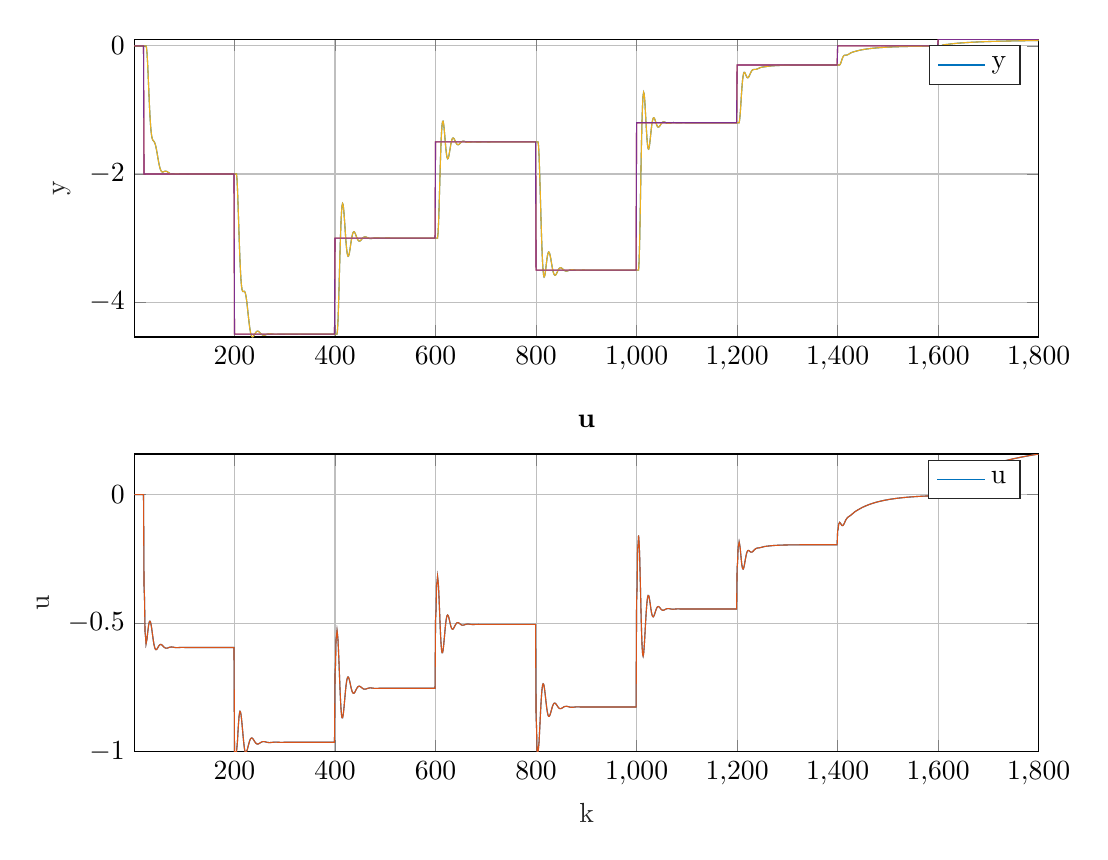
\begin{tikzpicture}

\begin{axis}[%
width=4.521in,
height=1.488in,
at={(0.758in,2.554in)},
scale only axis,
xmin=1,
xmax=1800,
ymin=-4.5439,
ymax=0.1,
ylabel style={font=\color{white!15!black}},
ylabel={y},
axis background/.style={fill=white},
xmajorgrids,
ymajorgrids,
legend style={legend cell align=left, align=left, draw=white!15!black}
]
\addplot [color=mycolor1]
  table[row sep=crcr]{%
1	0\\
2	0\\
3	0\\
4	0\\
5	0\\
6	0\\
7	0\\
8	0\\
9	0\\
10	0\\
11	0\\
12	0\\
13	0\\
14	0\\
15	0\\
16	0\\
17	0\\
18	0\\
19	0\\
20	0\\
21	0\\
22	0\\
23	0\\
24	0\\
25	-0.033091\\
26	-0.11817\\
27	-0.25132\\
28	-0.41963\\
29	-0.60589\\
30	-0.79286\\
31	-0.96661\\
32	-1.1171\\
33	-1.239\\
34	-1.3311\\
35	-1.3957\\
36	-1.4374\\
37	-1.4621\\
38	-1.4762\\
39	-1.4856\\
40	-1.4951\\
41	-1.5086\\
42	-1.5283\\
43	-1.5551\\
44	-1.5891\\
45	-1.629\\
46	-1.6733\\
47	-1.7197\\
48	-1.7661\\
49	-1.8104\\
50	-1.8508\\
51	-1.8859\\
52	-1.9148\\
53	-1.9371\\
54	-1.9531\\
55	-1.9632\\
56	-1.9684\\
57	-1.9697\\
58	-1.9683\\
59	-1.9654\\
60	-1.962\\
61	-1.9589\\
62	-1.9568\\
63	-1.9561\\
64	-1.957\\
65	-1.9595\\
66	-1.9633\\
67	-1.9681\\
68	-1.9736\\
69	-1.9794\\
70	-1.985\\
71	-1.9901\\
72	-1.9944\\
73	-1.9979\\
74	-2.0004\\
75	-2.0019\\
76	-2.0025\\
77	-2.0023\\
78	-2.0016\\
79	-2.0005\\
80	-1.9992\\
81	-1.9979\\
82	-1.9968\\
83	-1.9959\\
84	-1.9953\\
85	-1.9951\\
86	-1.9952\\
87	-1.9956\\
88	-1.9962\\
89	-1.9969\\
90	-1.9978\\
91	-1.9986\\
92	-1.9994\\
93	-2\\
94	-2.0005\\
95	-2.0009\\
96	-2.001\\
97	-2.0011\\
98	-2.001\\
99	-2.0008\\
100	-2.0005\\
101	-2.0002\\
102	-1.9999\\
103	-1.9997\\
104	-1.9995\\
105	-1.9994\\
106	-1.9993\\
107	-1.9993\\
108	-1.9993\\
109	-1.9994\\
110	-1.9996\\
111	-1.9997\\
112	-1.9998\\
113	-2\\
114	-2.0001\\
115	-2.0002\\
116	-2.0002\\
117	-2.0002\\
118	-2.0002\\
119	-2.0002\\
120	-2.0002\\
121	-2.0001\\
122	-2.0001\\
123	-2\\
124	-2\\
125	-1.9999\\
126	-1.9999\\
127	-1.9999\\
128	-1.9999\\
129	-1.9999\\
130	-1.9999\\
131	-1.9999\\
132	-2\\
133	-2\\
134	-2\\
135	-2\\
136	-2\\
137	-2\\
138	-2\\
139	-2\\
140	-2\\
141	-2\\
142	-2\\
143	-2\\
144	-2\\
145	-2\\
146	-2\\
147	-2\\
148	-2\\
149	-2\\
150	-2\\
151	-2\\
152	-2\\
153	-2\\
154	-2\\
155	-2\\
156	-2\\
157	-2\\
158	-2\\
159	-2\\
160	-2\\
161	-2\\
162	-2\\
163	-2\\
164	-2\\
165	-2\\
166	-2\\
167	-2\\
168	-2\\
169	-2\\
170	-2\\
171	-2\\
172	-2\\
173	-2\\
174	-2\\
175	-2\\
176	-2\\
177	-2\\
178	-2\\
179	-2\\
180	-2\\
181	-2\\
182	-2\\
183	-2\\
184	-2\\
185	-2\\
186	-2\\
187	-2\\
188	-2\\
189	-2\\
190	-2\\
191	-2\\
192	-2\\
193	-2\\
194	-2\\
195	-2\\
196	-2\\
197	-2\\
198	-2\\
199	-2\\
200	-2\\
201	-2\\
202	-2\\
203	-2\\
204	-2\\
205	-2.0801\\
206	-2.2463\\
207	-2.4603\\
208	-2.6956\\
209	-2.9345\\
210	-3.1613\\
211	-3.364\\
212	-3.5323\\
213	-3.6606\\
214	-3.7491\\
215	-3.8022\\
216	-3.8276\\
217	-3.8347\\
218	-3.8326\\
219	-3.8296\\
220	-3.8324\\
221	-3.8457\\
222	-3.8721\\
223	-3.9124\\
224	-3.9656\\
225	-4.0297\\
226	-4.1014\\
227	-4.1759\\
228	-4.249\\
229	-4.3177\\
230	-4.3797\\
231	-4.4329\\
232	-4.4759\\
233	-4.5081\\
234	-4.5296\\
235	-4.5411\\
236	-4.5439\\
237	-4.5397\\
238	-4.5303\\
239	-4.5176\\
240	-4.5034\\
241	-4.4891\\
242	-4.4762\\
243	-4.4656\\
244	-4.4579\\
245	-4.4535\\
246	-4.4523\\
247	-4.4541\\
248	-4.4584\\
249	-4.4647\\
250	-4.4723\\
251	-4.4806\\
252	-4.4888\\
253	-4.4966\\
254	-4.5033\\
255	-4.5088\\
256	-4.5128\\
257	-4.5153\\
258	-4.5163\\
259	-4.516\\
260	-4.5146\\
261	-4.5123\\
262	-4.5095\\
263	-4.5064\\
264	-4.5032\\
265	-4.5003\\
266	-4.4977\\
267	-4.4957\\
268	-4.4943\\
269	-4.4934\\
270	-4.4932\\
271	-4.4934\\
272	-4.4941\\
273	-4.4951\\
274	-4.4963\\
275	-4.4976\\
276	-4.4989\\
277	-4.5001\\
278	-4.5011\\
279	-4.5019\\
280	-4.5024\\
281	-4.5027\\
282	-4.5028\\
283	-4.5026\\
284	-4.5023\\
285	-4.5019\\
286	-4.5014\\
287	-4.5009\\
288	-4.5004\\
289	-4.4999\\
290	-4.4995\\
291	-4.4992\\
292	-4.499\\
293	-4.4989\\
294	-4.4989\\
295	-4.4989\\
296	-4.4991\\
297	-4.4993\\
298	-4.4995\\
299	-4.4997\\
300	-4.4999\\
301	-4.5001\\
302	-4.5002\\
303	-4.5003\\
304	-4.5004\\
305	-4.5005\\
306	-4.5005\\
307	-4.5004\\
308	-4.5004\\
309	-4.5003\\
310	-4.5002\\
311	-4.5001\\
312	-4.5\\
313	-4.5\\
314	-4.4999\\
315	-4.4999\\
316	-4.4998\\
317	-4.4998\\
318	-4.4998\\
319	-4.4998\\
320	-4.4999\\
321	-4.4999\\
322	-4.4999\\
323	-4.5\\
324	-4.5\\
325	-4.5\\
326	-4.5\\
327	-4.5001\\
328	-4.5001\\
329	-4.5001\\
330	-4.5001\\
331	-4.5001\\
332	-4.5001\\
333	-4.5\\
334	-4.5\\
335	-4.5\\
336	-4.5\\
337	-4.5\\
338	-4.5\\
339	-4.5\\
340	-4.5\\
341	-4.5\\
342	-4.5\\
343	-4.5\\
344	-4.5\\
345	-4.5\\
346	-4.5\\
347	-4.5\\
348	-4.5\\
349	-4.5\\
350	-4.5\\
351	-4.5\\
352	-4.5\\
353	-4.5\\
354	-4.5\\
355	-4.5\\
356	-4.5\\
357	-4.5\\
358	-4.5\\
359	-4.5\\
360	-4.5\\
361	-4.5\\
362	-4.5\\
363	-4.5\\
364	-4.5\\
365	-4.5\\
366	-4.5\\
367	-4.5\\
368	-4.5\\
369	-4.5\\
370	-4.5\\
371	-4.5\\
372	-4.5\\
373	-4.5\\
374	-4.5\\
375	-4.5\\
376	-4.5\\
377	-4.5\\
378	-4.5\\
379	-4.5\\
380	-4.5\\
381	-4.5\\
382	-4.5\\
383	-4.5\\
384	-4.5\\
385	-4.5\\
386	-4.5\\
387	-4.5\\
388	-4.5\\
389	-4.5\\
390	-4.5\\
391	-4.5\\
392	-4.5\\
393	-4.5\\
394	-4.5\\
395	-4.5\\
396	-4.5\\
397	-4.5\\
398	-4.5\\
399	-4.5\\
400	-4.5\\
401	-4.5\\
402	-4.5\\
403	-4.5\\
404	-4.5\\
405	-4.4276\\
406	-4.2775\\
407	-4.0508\\
408	-3.7775\\
409	-3.4837\\
410	-3.199\\
411	-2.9452\\
412	-2.7384\\
413	-2.5876\\
414	-2.4958\\
415	-2.4608\\
416	-2.4768\\
417	-2.5349\\
418	-2.6243\\
419	-2.7338\\
420	-2.8519\\
421	-2.9682\\
422	-3.0738\\
423	-3.1618\\
424	-3.2275\\
425	-3.2686\\
426	-3.2851\\
427	-3.2789\\
428	-3.2535\\
429	-3.2133\\
430	-3.1637\\
431	-3.1096\\
432	-3.056\\
433	-3.007\\
434	-2.9656\\
435	-2.9339\\
436	-2.9129\\
437	-2.9026\\
438	-2.9021\\
439	-2.9101\\
440	-2.9245\\
441	-2.9433\\
442	-2.9644\\
443	-2.9855\\
444	-3.0052\\
445	-3.0219\\
446	-3.0348\\
447	-3.0433\\
448	-3.0473\\
449	-3.0473\\
450	-3.0436\\
451	-3.0372\\
452	-3.0289\\
453	-3.0196\\
454	-3.0102\\
455	-3.0014\\
456	-2.9938\\
457	-2.9879\\
458	-2.9838\\
459	-2.9817\\
460	-2.9814\\
461	-2.9826\\
462	-2.985\\
463	-2.9883\\
464	-2.9921\\
465	-2.996\\
466	-2.9996\\
467	-3.0028\\
468	-3.0053\\
469	-3.0071\\
470	-3.008\\
471	-3.0082\\
472	-3.0077\\
473	-3.0067\\
474	-3.0053\\
475	-3.0037\\
476	-3.002\\
477	-3.0005\\
478	-2.9991\\
479	-2.998\\
480	-2.9972\\
481	-2.9967\\
482	-2.9966\\
483	-2.9968\\
484	-2.9972\\
485	-2.9977\\
486	-2.9984\\
487	-2.9991\\
488	-2.9998\\
489	-3.0004\\
490	-3.0008\\
491	-3.0012\\
492	-3.0014\\
493	-3.0014\\
494	-3.0014\\
495	-3.0012\\
496	-3.001\\
497	-3.0007\\
498	-3.0004\\
499	-3.0001\\
500	-2.9999\\
501	-2.9997\\
502	-2.9995\\
503	-2.9994\\
504	-2.9994\\
505	-2.9994\\
506	-2.9995\\
507	-2.9996\\
508	-2.9997\\
509	-2.9998\\
510	-2.9999\\
511	-3\\
512	-3.0001\\
513	-3.0002\\
514	-3.0002\\
515	-3.0003\\
516	-3.0003\\
517	-3.0002\\
518	-3.0002\\
519	-3.0001\\
520	-3.0001\\
521	-3\\
522	-3\\
523	-2.9999\\
524	-2.9999\\
525	-2.9999\\
526	-2.9999\\
527	-2.9999\\
528	-2.9999\\
529	-2.9999\\
530	-2.9999\\
531	-3\\
532	-3\\
533	-3\\
534	-3\\
535	-3\\
536	-3\\
537	-3\\
538	-3\\
539	-3\\
540	-3\\
541	-3\\
542	-3\\
543	-3\\
544	-3\\
545	-3\\
546	-3\\
547	-3\\
548	-3\\
549	-3\\
550	-3\\
551	-3\\
552	-3\\
553	-3\\
554	-3\\
555	-3\\
556	-3\\
557	-3\\
558	-3\\
559	-3\\
560	-3\\
561	-3\\
562	-3\\
563	-3\\
564	-3\\
565	-3\\
566	-3\\
567	-3\\
568	-3\\
569	-3\\
570	-3\\
571	-3\\
572	-3\\
573	-3\\
574	-3\\
575	-3\\
576	-3\\
577	-3\\
578	-3\\
579	-3\\
580	-3\\
581	-3\\
582	-3\\
583	-3\\
584	-3\\
585	-3\\
586	-3\\
587	-3\\
588	-3\\
589	-3\\
590	-3\\
591	-3\\
592	-3\\
593	-3\\
594	-3\\
595	-3\\
596	-3\\
597	-3\\
598	-3\\
599	-3\\
600	-3\\
601	-3\\
602	-3\\
603	-3\\
604	-3\\
605	-2.9213\\
606	-2.7643\\
607	-2.5318\\
608	-2.2611\\
609	-1.9817\\
610	-1.7237\\
611	-1.5062\\
612	-1.3411\\
613	-1.2326\\
614	-1.1795\\
615	-1.1761\\
616	-1.2141\\
617	-1.2827\\
618	-1.3706\\
619	-1.4661\\
620	-1.5589\\
621	-1.64\\
622	-1.7031\\
623	-1.7443\\
624	-1.7622\\
625	-1.7582\\
626	-1.7353\\
627	-1.6983\\
628	-1.6525\\
629	-1.6033\\
630	-1.5557\\
631	-1.5135\\
632	-1.4796\\
633	-1.4556\\
634	-1.4419\\
635	-1.4379\\
636	-1.4423\\
637	-1.4531\\
638	-1.4681\\
639	-1.4852\\
640	-1.5023\\
641	-1.5177\\
642	-1.53\\
643	-1.5385\\
644	-1.5428\\
645	-1.5432\\
646	-1.5401\\
647	-1.5343\\
648	-1.5268\\
649	-1.5183\\
650	-1.5099\\
651	-1.5023\\
652	-1.4961\\
653	-1.4915\\
654	-1.4887\\
655	-1.4877\\
656	-1.4882\\
657	-1.49\\
658	-1.4926\\
659	-1.4957\\
660	-1.4988\\
661	-1.5017\\
662	-1.5041\\
663	-1.5059\\
664	-1.5069\\
665	-1.5072\\
666	-1.5068\\
667	-1.5059\\
668	-1.5047\\
669	-1.5033\\
670	-1.5018\\
671	-1.5004\\
672	-1.4993\\
673	-1.4984\\
674	-1.4979\\
675	-1.4976\\
676	-1.4977\\
677	-1.498\\
678	-1.4984\\
679	-1.499\\
680	-1.4996\\
681	-1.5001\\
682	-1.5006\\
683	-1.5009\\
684	-1.5011\\
685	-1.5012\\
686	-1.5012\\
687	-1.501\\
688	-1.5008\\
689	-1.5006\\
690	-1.5003\\
691	-1.5001\\
692	-1.4999\\
693	-1.4997\\
694	-1.4996\\
695	-1.4996\\
696	-1.4996\\
697	-1.4996\\
698	-1.4997\\
699	-1.4998\\
700	-1.4999\\
701	-1.5\\
702	-1.5001\\
703	-1.5001\\
704	-1.5002\\
705	-1.5002\\
706	-1.5002\\
707	-1.5002\\
708	-1.5002\\
709	-1.5001\\
710	-1.5001\\
711	-1.5\\
712	-1.5\\
713	-1.5\\
714	-1.4999\\
715	-1.4999\\
716	-1.4999\\
717	-1.4999\\
718	-1.4999\\
719	-1.5\\
720	-1.5\\
721	-1.5\\
722	-1.5\\
723	-1.5\\
724	-1.5\\
725	-1.5\\
726	-1.5\\
727	-1.5\\
728	-1.5\\
729	-1.5\\
730	-1.5\\
731	-1.5\\
732	-1.5\\
733	-1.5\\
734	-1.5\\
735	-1.5\\
736	-1.5\\
737	-1.5\\
738	-1.5\\
739	-1.5\\
740	-1.5\\
741	-1.5\\
742	-1.5\\
743	-1.5\\
744	-1.5\\
745	-1.5\\
746	-1.5\\
747	-1.5\\
748	-1.5\\
749	-1.5\\
750	-1.5\\
751	-1.5\\
752	-1.5\\
753	-1.5\\
754	-1.5\\
755	-1.5\\
756	-1.5\\
757	-1.5\\
758	-1.5\\
759	-1.5\\
760	-1.5\\
761	-1.5\\
762	-1.5\\
763	-1.5\\
764	-1.5\\
765	-1.5\\
766	-1.5\\
767	-1.5\\
768	-1.5\\
769	-1.5\\
770	-1.5\\
771	-1.5\\
772	-1.5\\
773	-1.5\\
774	-1.5\\
775	-1.5\\
776	-1.5\\
777	-1.5\\
778	-1.5\\
779	-1.5\\
780	-1.5\\
781	-1.5\\
782	-1.5\\
783	-1.5\\
784	-1.5\\
785	-1.5\\
786	-1.5\\
787	-1.5\\
788	-1.5\\
789	-1.5\\
790	-1.5\\
791	-1.5\\
792	-1.5\\
793	-1.5\\
794	-1.5\\
795	-1.5\\
796	-1.5\\
797	-1.5\\
798	-1.5\\
799	-1.5\\
800	-1.5\\
801	-1.5\\
802	-1.5\\
803	-1.5\\
804	-1.5\\
805	-1.57\\
806	-1.723\\
807	-1.9423\\
808	-2.2031\\
809	-2.4793\\
810	-2.7501\\
811	-2.9998\\
812	-3.2147\\
813	-3.3855\\
814	-3.5072\\
815	-3.5798\\
816	-3.6073\\
817	-3.5969\\
818	-3.5577\\
819	-3.4999\\
820	-3.4332\\
821	-3.3667\\
822	-3.3074\\
823	-3.2608\\
824	-3.2301\\
825	-3.2167\\
826	-3.2202\\
827	-3.239\\
828	-3.2703\\
829	-3.3106\\
830	-3.3562\\
831	-3.4036\\
832	-3.4493\\
833	-3.4906\\
834	-3.5252\\
835	-3.5517\\
836	-3.5696\\
837	-3.5788\\
838	-3.5801\\
839	-3.5745\\
840	-3.5636\\
841	-3.5491\\
842	-3.5326\\
843	-3.5158\\
844	-3.4999\\
845	-3.4862\\
846	-3.4754\\
847	-3.4679\\
848	-3.4638\\
849	-3.463\\
850	-3.465\\
851	-3.4694\\
852	-3.4754\\
853	-3.4825\\
854	-3.4898\\
855	-3.4969\\
856	-3.5032\\
857	-3.5083\\
858	-3.5121\\
859	-3.5144\\
860	-3.5153\\
861	-3.515\\
862	-3.5135\\
863	-3.5112\\
864	-3.5084\\
865	-3.5054\\
866	-3.5024\\
867	-3.4996\\
868	-3.4973\\
869	-3.4955\\
870	-3.4943\\
871	-3.4937\\
872	-3.4937\\
873	-3.4941\\
874	-3.4949\\
875	-3.4961\\
876	-3.4973\\
877	-3.4986\\
878	-3.4998\\
879	-3.5008\\
880	-3.5017\\
881	-3.5023\\
882	-3.5026\\
883	-3.5027\\
884	-3.5026\\
885	-3.5023\\
886	-3.5018\\
887	-3.5013\\
888	-3.5008\\
889	-3.5003\\
890	-3.4998\\
891	-3.4994\\
892	-3.4991\\
893	-3.499\\
894	-3.4989\\
895	-3.4989\\
896	-3.499\\
897	-3.4992\\
898	-3.4994\\
899	-3.4996\\
900	-3.4998\\
901	-3.5\\
902	-3.5002\\
903	-3.5003\\
904	-3.5004\\
905	-3.5005\\
906	-3.5005\\
907	-3.5004\\
908	-3.5004\\
909	-3.5003\\
910	-3.5002\\
911	-3.5001\\
912	-3.5\\
913	-3.4999\\
914	-3.4999\\
915	-3.4998\\
916	-3.4998\\
917	-3.4998\\
918	-3.4998\\
919	-3.4998\\
920	-3.4999\\
921	-3.4999\\
922	-3.4999\\
923	-3.5\\
924	-3.5\\
925	-3.5\\
926	-3.5001\\
927	-3.5001\\
928	-3.5001\\
929	-3.5001\\
930	-3.5001\\
931	-3.5001\\
932	-3.5\\
933	-3.5\\
934	-3.5\\
935	-3.5\\
936	-3.5\\
937	-3.5\\
938	-3.5\\
939	-3.5\\
940	-3.5\\
941	-3.5\\
942	-3.5\\
943	-3.5\\
944	-3.5\\
945	-3.5\\
946	-3.5\\
947	-3.5\\
948	-3.5\\
949	-3.5\\
950	-3.5\\
951	-3.5\\
952	-3.5\\
953	-3.5\\
954	-3.5\\
955	-3.5\\
956	-3.5\\
957	-3.5\\
958	-3.5\\
959	-3.5\\
960	-3.5\\
961	-3.5\\
962	-3.5\\
963	-3.5\\
964	-3.5\\
965	-3.5\\
966	-3.5\\
967	-3.5\\
968	-3.5\\
969	-3.5\\
970	-3.5\\
971	-3.5\\
972	-3.5\\
973	-3.5\\
974	-3.5\\
975	-3.5\\
976	-3.5\\
977	-3.5\\
978	-3.5\\
979	-3.5\\
980	-3.5\\
981	-3.5\\
982	-3.5\\
983	-3.5\\
984	-3.5\\
985	-3.5\\
986	-3.5\\
987	-3.5\\
988	-3.5\\
989	-3.5\\
990	-3.5\\
991	-3.5\\
992	-3.5\\
993	-3.5\\
994	-3.5\\
995	-3.5\\
996	-3.5\\
997	-3.5\\
998	-3.5\\
999	-3.5\\
1000	-3.5\\
1001	-3.5\\
1002	-3.5\\
1003	-3.5\\
1004	-3.5\\
1005	-3.365\\
1006	-3.0998\\
1007	-2.7034\\
1008	-2.2557\\
1009	-1.8131\\
1010	-1.426\\
1011	-1.1185\\
1012	-0.90054\\
1013	-0.77118\\
1014	-0.72397\\
1015	-0.74789\\
1016	-0.82844\\
1017	-0.94867\\
1018	-1.0906\\
1019	-1.2368\\
1020	-1.3717\\
1021	-1.483\\
1022	-1.5622\\
1023	-1.6051\\
1024	-1.6117\\
1025	-1.5861\\
1026	-1.5351\\
1027	-1.4673\\
1028	-1.3918\\
1029	-1.317\\
1030	-1.2498\\
1031	-1.1949\\
1032	-1.1551\\
1033	-1.1314\\
1034	-1.1228\\
1035	-1.1273\\
1036	-1.1421\\
1037	-1.1635\\
1038	-1.1883\\
1039	-1.213\\
1040	-1.2351\\
1041	-1.2525\\
1042	-1.2641\\
1043	-1.2694\\
1044	-1.2687\\
1045	-1.2629\\
1046	-1.2533\\
1047	-1.2413\\
1048	-1.2284\\
1049	-1.216\\
1050	-1.205\\
1051	-1.1963\\
1052	-1.1902\\
1053	-1.1868\\
1054	-1.186\\
1055	-1.1874\\
1056	-1.1903\\
1057	-1.1943\\
1058	-1.1986\\
1059	-1.2028\\
1060	-1.2064\\
1061	-1.2091\\
1062	-1.2108\\
1063	-1.2114\\
1064	-1.211\\
1065	-1.2099\\
1066	-1.2081\\
1067	-1.206\\
1068	-1.2039\\
1069	-1.2018\\
1070	-1.2001\\
1071	-1.1988\\
1072	-1.1979\\
1073	-1.1975\\
1074	-1.1975\\
1075	-1.1978\\
1076	-1.1984\\
1077	-1.1991\\
1078	-1.1999\\
1079	-1.2006\\
1080	-1.2011\\
1081	-1.2016\\
1082	-1.2018\\
1083	-1.2019\\
1084	-1.2018\\
1085	-1.2015\\
1086	-1.2012\\
1087	-1.2009\\
1088	-1.2005\\
1089	-1.2002\\
1090	-1.1999\\
1091	-1.1997\\
1092	-1.1996\\
1093	-1.1995\\
1094	-1.1996\\
1095	-1.1996\\
1096	-1.1997\\
1097	-1.1999\\
1098	-1.2\\
1099	-1.2001\\
1100	-1.2002\\
1101	-1.2003\\
1102	-1.2003\\
1103	-1.2003\\
1104	-1.2003\\
1105	-1.2002\\
1106	-1.2002\\
1107	-1.2001\\
1108	-1.2001\\
1109	-1.2\\
1110	-1.2\\
1111	-1.1999\\
1112	-1.1999\\
1113	-1.1999\\
1114	-1.1999\\
1115	-1.1999\\
1116	-1.2\\
1117	-1.2\\
1118	-1.2\\
1119	-1.2\\
1120	-1.2\\
1121	-1.2\\
1122	-1.2\\
1123	-1.2\\
1124	-1.2\\
1125	-1.2\\
1126	-1.2\\
1127	-1.2\\
1128	-1.2\\
1129	-1.2\\
1130	-1.2\\
1131	-1.2\\
1132	-1.2\\
1133	-1.2\\
1134	-1.2\\
1135	-1.2\\
1136	-1.2\\
1137	-1.2\\
1138	-1.2\\
1139	-1.2\\
1140	-1.2\\
1141	-1.2\\
1142	-1.2\\
1143	-1.2\\
1144	-1.2\\
1145	-1.2\\
1146	-1.2\\
1147	-1.2\\
1148	-1.2\\
1149	-1.2\\
1150	-1.2\\
1151	-1.2\\
1152	-1.2\\
1153	-1.2\\
1154	-1.2\\
1155	-1.2\\
1156	-1.2\\
1157	-1.2\\
1158	-1.2\\
1159	-1.2\\
1160	-1.2\\
1161	-1.2\\
1162	-1.2\\
1163	-1.2\\
1164	-1.2\\
1165	-1.2\\
1166	-1.2\\
1167	-1.2\\
1168	-1.2\\
1169	-1.2\\
1170	-1.2\\
1171	-1.2\\
1172	-1.2\\
1173	-1.2\\
1174	-1.2\\
1175	-1.2\\
1176	-1.2\\
1177	-1.2\\
1178	-1.2\\
1179	-1.2\\
1180	-1.2\\
1181	-1.2\\
1182	-1.2\\
1183	-1.2\\
1184	-1.2\\
1185	-1.2\\
1186	-1.2\\
1187	-1.2\\
1188	-1.2\\
1189	-1.2\\
1190	-1.2\\
1191	-1.2\\
1192	-1.2\\
1193	-1.2\\
1194	-1.2\\
1195	-1.2\\
1196	-1.2\\
1197	-1.2\\
1198	-1.2\\
1199	-1.2\\
1200	-1.2\\
1201	-1.2\\
1202	-1.2\\
1203	-1.2\\
1204	-1.2\\
1205	-1.1571\\
1206	-1.0755\\
1207	-0.96297\\
1208	-0.83898\\
1209	-0.71797\\
1210	-0.61185\\
1211	-0.52709\\
1212	-0.46647\\
1213	-0.42953\\
1214	-0.4136\\
1215	-0.41445\\
1216	-0.42698\\
1217	-0.44584\\
1218	-0.46602\\
1219	-0.48342\\
1220	-0.49513\\
1221	-0.49961\\
1222	-0.49668\\
1223	-0.48722\\
1224	-0.47285\\
1225	-0.45555\\
1226	-0.4373\\
1227	-0.41979\\
1228	-0.40431\\
1229	-0.39164\\
1230	-0.38208\\
1231	-0.3755\\
1232	-0.37149\\
1233	-0.36942\\
1234	-0.3686\\
1235	-0.36837\\
1236	-0.36814\\
1237	-0.36749\\
1238	-0.36619\\
1239	-0.36414\\
1240	-0.3614\\
1241	-0.35812\\
1242	-0.3545\\
1243	-0.35078\\
1244	-0.34715\\
1245	-0.34378\\
1246	-0.34077\\
1247	-0.33817\\
1248	-0.33598\\
1249	-0.33417\\
1250	-0.33265\\
1251	-0.33136\\
1252	-0.3302\\
1253	-0.32912\\
1254	-0.32804\\
1255	-0.32695\\
1256	-0.32583\\
1257	-0.32466\\
1258	-0.32348\\
1259	-0.32229\\
1260	-0.32113\\
1261	-0.32001\\
1262	-0.31895\\
1263	-0.31795\\
1264	-0.31704\\
1265	-0.31619\\
1266	-0.31542\\
1267	-0.31471\\
1268	-0.31405\\
1269	-0.31343\\
1270	-0.31284\\
1271	-0.31228\\
1272	-0.31173\\
1273	-0.3112\\
1274	-0.31069\\
1275	-0.31019\\
1276	-0.30971\\
1277	-0.30925\\
1278	-0.30881\\
1279	-0.30838\\
1280	-0.30798\\
1281	-0.30761\\
1282	-0.30725\\
1283	-0.30691\\
1284	-0.30659\\
1285	-0.30629\\
1286	-0.306\\
1287	-0.30573\\
1288	-0.30547\\
1289	-0.30522\\
1290	-0.30498\\
1291	-0.30475\\
1292	-0.30453\\
1293	-0.30432\\
1294	-0.30412\\
1295	-0.30393\\
1296	-0.30375\\
1297	-0.30358\\
1298	-0.30341\\
1299	-0.30325\\
1300	-0.3031\\
1301	-0.30296\\
1302	-0.30283\\
1303	-0.3027\\
1304	-0.30257\\
1305	-0.30245\\
1306	-0.30234\\
1307	-0.30223\\
1308	-0.30213\\
1309	-0.30203\\
1310	-0.30194\\
1311	-0.30185\\
1312	-0.30177\\
1313	-0.30169\\
1314	-0.30161\\
1315	-0.30153\\
1316	-0.30146\\
1317	-0.3014\\
1318	-0.30133\\
1319	-0.30127\\
1320	-0.30121\\
1321	-0.30116\\
1322	-0.3011\\
1323	-0.30105\\
1324	-0.30101\\
1325	-0.30096\\
1326	-0.30092\\
1327	-0.30087\\
1328	-0.30083\\
1329	-0.3008\\
1330	-0.30076\\
1331	-0.30072\\
1332	-0.30069\\
1333	-0.30066\\
1334	-0.30063\\
1335	-0.3006\\
1336	-0.30057\\
1337	-0.30055\\
1338	-0.30052\\
1339	-0.3005\\
1340	-0.30048\\
1341	-0.30045\\
1342	-0.30043\\
1343	-0.30041\\
1344	-0.30039\\
1345	-0.30038\\
1346	-0.30036\\
1347	-0.30034\\
1348	-0.30033\\
1349	-0.30031\\
1350	-0.3003\\
1351	-0.30028\\
1352	-0.30027\\
1353	-0.30026\\
1354	-0.30025\\
1355	-0.30024\\
1356	-0.30022\\
1357	-0.30021\\
1358	-0.3002\\
1359	-0.3002\\
1360	-0.30019\\
1361	-0.30018\\
1362	-0.30017\\
1363	-0.30016\\
1364	-0.30015\\
1365	-0.30015\\
1366	-0.30014\\
1367	-0.30013\\
1368	-0.30013\\
1369	-0.30012\\
1370	-0.30012\\
1371	-0.30011\\
1372	-0.30011\\
1373	-0.3001\\
1374	-0.3001\\
1375	-0.30009\\
1376	-0.30009\\
1377	-0.30008\\
1378	-0.30008\\
1379	-0.30008\\
1380	-0.30007\\
1381	-0.30007\\
1382	-0.30007\\
1383	-0.30006\\
1384	-0.30006\\
1385	-0.30006\\
1386	-0.30006\\
1387	-0.30005\\
1388	-0.30005\\
1389	-0.30005\\
1390	-0.30005\\
1391	-0.30004\\
1392	-0.30004\\
1393	-0.30004\\
1394	-0.30004\\
1395	-0.30004\\
1396	-0.30003\\
1397	-0.30003\\
1398	-0.30003\\
1399	-0.30003\\
1400	-0.30003\\
1401	-0.30003\\
1402	-0.30003\\
1403	-0.30002\\
1404	-0.30002\\
1405	-0.29124\\
1406	-0.27427\\
1407	-0.25175\\
1408	-0.22747\\
1409	-0.20438\\
1410	-0.18458\\
1411	-0.1691\\
1412	-0.15815\\
1413	-0.15125\\
1414	-0.14753\\
1415	-0.14592\\
1416	-0.14536\\
1417	-0.14493\\
1418	-0.14397\\
1419	-0.14209\\
1420	-0.13918\\
1421	-0.13535\\
1422	-0.13084\\
1423	-0.12596\\
1424	-0.121\\
1425	-0.11622\\
1426	-0.1118\\
1427	-0.10782\\
1428	-0.10432\\
1429	-0.10124\\
1430	-0.098511\\
1431	-0.096042\\
1432	-0.09374\\
1433	-0.091528\\
1434	-0.089352\\
1435	-0.087177\\
1436	-0.084995\\
1437	-0.082811\\
1438	-0.080641\\
1439	-0.078506\\
1440	-0.076424\\
1441	-0.074414\\
1442	-0.072483\\
1443	-0.070637\\
1444	-0.068874\\
1445	-0.067187\\
1446	-0.06557\\
1447	-0.064013\\
1448	-0.062508\\
1449	-0.061048\\
1450	-0.059628\\
1451	-0.058244\\
1452	-0.056896\\
1453	-0.055582\\
1454	-0.054303\\
1455	-0.053058\\
1456	-0.051848\\
1457	-0.050673\\
1458	-0.049532\\
1459	-0.048425\\
1460	-0.04735\\
1461	-0.046305\\
1462	-0.04529\\
1463	-0.044303\\
1464	-0.043342\\
1465	-0.042407\\
1466	-0.041496\\
1467	-0.040608\\
1468	-0.039743\\
1469	-0.0389\\
1470	-0.038078\\
1471	-0.037277\\
1472	-0.036497\\
1473	-0.035735\\
1474	-0.034993\\
1475	-0.03427\\
1476	-0.033564\\
1477	-0.032875\\
1478	-0.032203\\
1479	-0.031548\\
1480	-0.030908\\
1481	-0.030283\\
1482	-0.029673\\
1483	-0.029078\\
1484	-0.028496\\
1485	-0.027928\\
1486	-0.027373\\
1487	-0.02683\\
1488	-0.0263\\
1489	-0.025783\\
1490	-0.025277\\
1491	-0.024782\\
1492	-0.024298\\
1493	-0.023826\\
1494	-0.023363\\
1495	-0.022911\\
1496	-0.022469\\
1497	-0.022037\\
1498	-0.021614\\
1499	-0.0212\\
1500	-0.020795\\
1501	-0.020399\\
1502	-0.020011\\
1503	-0.019631\\
1504	-0.01926\\
1505	-0.018897\\
1506	-0.018541\\
1507	-0.018192\\
1508	-0.017851\\
1509	-0.017517\\
1510	-0.01719\\
1511	-0.01687\\
1512	-0.016556\\
1513	-0.016249\\
1514	-0.015948\\
1515	-0.015653\\
1516	-0.015364\\
1517	-0.015081\\
1518	-0.014804\\
1519	-0.014532\\
1520	-0.014266\\
1521	-0.014005\\
1522	-0.013749\\
1523	-0.013498\\
1524	-0.013253\\
1525	-0.013012\\
1526	-0.012776\\
1527	-0.012544\\
1528	-0.012317\\
1529	-0.012095\\
1530	-0.011877\\
1531	-0.011663\\
1532	-0.011453\\
1533	-0.011247\\
1534	-0.011046\\
1535	-0.010848\\
1536	-0.010654\\
1537	-0.010463\\
1538	-0.010277\\
1539	-0.010094\\
1540	-0.0099138\\
1541	-0.0097376\\
1542	-0.0095647\\
1543	-0.009395\\
1544	-0.0092285\\
1545	-0.0090652\\
1546	-0.0089049\\
1547	-0.0087477\\
1548	-0.0085934\\
1549	-0.0084419\\
1550	-0.0082933\\
1551	-0.0081474\\
1552	-0.0080043\\
1553	-0.0078638\\
1554	-0.0077259\\
1555	-0.0075905\\
1556	-0.0074577\\
1557	-0.0073272\\
1558	-0.0071992\\
1559	-0.0070735\\
1560	-0.0069502\\
1561	-0.006829\\
1562	-0.0067101\\
1563	-0.0065934\\
1564	-0.0064787\\
1565	-0.0063662\\
1566	-0.0062557\\
1567	-0.0061472\\
1568	-0.0060406\\
1569	-0.005936\\
1570	-0.0058333\\
1571	-0.0057324\\
1572	-0.0056333\\
1573	-0.005536\\
1574	-0.0054405\\
1575	-0.0053466\\
1576	-0.0052545\\
1577	-0.005164\\
1578	-0.0050751\\
1579	-0.0049877\\
1580	-0.004902\\
1581	-0.0048178\\
1582	-0.004735\\
1583	-0.0046537\\
1584	-0.0045739\\
1585	-0.0044955\\
1586	-0.0044185\\
1587	-0.0043428\\
1588	-0.0042685\\
1589	-0.0041954\\
1590	-0.0041237\\
1591	-0.0040532\\
1592	-0.003984\\
1593	-0.0039159\\
1594	-0.0038491\\
1595	-0.0037835\\
1596	-0.0037189\\
1597	-0.0036556\\
1598	-0.0035933\\
1599	-0.0035321\\
1600	-0.003472\\
1601	-0.0034129\\
1602	-0.0033549\\
1603	-0.0032979\\
1604	-0.0032418\\
1605	-0.0020376\\
1606	0.00060101\\
1607	0.0040024\\
1608	0.0076369\\
1609	0.010979\\
1610	0.013768\\
1611	0.015888\\
1612	0.017394\\
1613	0.018417\\
1614	0.019134\\
1615	0.019715\\
1616	0.020298\\
1617	0.020972\\
1618	0.021779\\
1619	0.022719\\
1620	0.023764\\
1621	0.024874\\
1622	0.026005\\
1623	0.02712\\
1624	0.028194\\
1625	0.029212\\
1626	0.030171\\
1627	0.031076\\
1628	0.031937\\
1629	0.032765\\
1630	0.033569\\
1631	0.034359\\
1632	0.035139\\
1633	0.03591\\
1634	0.036675\\
1635	0.03743\\
1636	0.038175\\
1637	0.038907\\
1638	0.039625\\
1639	0.040327\\
1640	0.041014\\
1641	0.041686\\
1642	0.042343\\
1643	0.042987\\
1644	0.043619\\
1645	0.044238\\
1646	0.044846\\
1647	0.045444\\
1648	0.046031\\
1649	0.046608\\
1650	0.047175\\
1651	0.047733\\
1652	0.04828\\
1653	0.048819\\
1654	0.049347\\
1655	0.049867\\
1656	0.050378\\
1657	0.05088\\
1658	0.051374\\
1659	0.051859\\
1660	0.052337\\
1661	0.052807\\
1662	0.053269\\
1663	0.053724\\
1664	0.054171\\
1665	0.054612\\
1666	0.055045\\
1667	0.055472\\
1668	0.055892\\
1669	0.056306\\
1670	0.056713\\
1671	0.057115\\
1672	0.05751\\
1673	0.057899\\
1674	0.058282\\
1675	0.05866\\
1676	0.059033\\
1677	0.059399\\
1678	0.059761\\
1679	0.060117\\
1680	0.060468\\
1681	0.060815\\
1682	0.061156\\
1683	0.061493\\
1684	0.061825\\
1685	0.062152\\
1686	0.062475\\
1687	0.062793\\
1688	0.063107\\
1689	0.063417\\
1690	0.063723\\
1691	0.064024\\
1692	0.064322\\
1693	0.064615\\
1694	0.064905\\
1695	0.065191\\
1696	0.065474\\
1697	0.065752\\
1698	0.066028\\
1699	0.066299\\
1700	0.066568\\
1701	0.066832\\
1702	0.067094\\
1703	0.067352\\
1704	0.067607\\
1705	0.067859\\
1706	0.068108\\
1707	0.068354\\
1708	0.068597\\
1709	0.068837\\
1710	0.069074\\
1711	0.069308\\
1712	0.06954\\
1713	0.069768\\
1714	0.069995\\
1715	0.070218\\
1716	0.070439\\
1717	0.070657\\
1718	0.070873\\
1719	0.071086\\
1720	0.071297\\
1721	0.071506\\
1722	0.071712\\
1723	0.071916\\
1724	0.072118\\
1725	0.072317\\
1726	0.072514\\
1727	0.072709\\
1728	0.072902\\
1729	0.073093\\
1730	0.073282\\
1731	0.073469\\
1732	0.073653\\
1733	0.073836\\
1734	0.074017\\
1735	0.074196\\
1736	0.074373\\
1737	0.074548\\
1738	0.074722\\
1739	0.074893\\
1740	0.075063\\
1741	0.075231\\
1742	0.075397\\
1743	0.075562\\
1744	0.075725\\
1745	0.075886\\
1746	0.076046\\
1747	0.076204\\
1748	0.076361\\
1749	0.076516\\
1750	0.076669\\
1751	0.076821\\
1752	0.076972\\
1753	0.077121\\
1754	0.077269\\
1755	0.077415\\
1756	0.07756\\
1757	0.077703\\
1758	0.077845\\
1759	0.077986\\
1760	0.078125\\
1761	0.078263\\
1762	0.0784\\
1763	0.078535\\
1764	0.078669\\
1765	0.078802\\
1766	0.078934\\
1767	0.079065\\
1768	0.079194\\
1769	0.079322\\
1770	0.079449\\
1771	0.079575\\
1772	0.0797\\
1773	0.079823\\
1774	0.079946\\
1775	0.080067\\
1776	0.080187\\
1777	0.080307\\
1778	0.080425\\
1779	0.080542\\
1780	0.080658\\
1781	0.080773\\
1782	0.080887\\
1783	0.081\\
1784	0.081113\\
1785	0.081224\\
1786	0.081334\\
1787	0.081443\\
1788	0.081552\\
1789	0.081659\\
1790	0.081766\\
1791	0.081872\\
1792	0.081976\\
1793	0.08208\\
1794	0.082183\\
1795	0.082286\\
1796	0.082387\\
1797	0.082487\\
1798	0.082587\\
1799	0.082686\\
1800	0.082784\\
};
\addlegendentry{y}

\addplot [color=mycolor2, forget plot]
  table[row sep=crcr]{%
1	0\\
2	0\\
3	0\\
4	0\\
5	0\\
6	0\\
7	0\\
8	0\\
9	0\\
10	0\\
11	0\\
12	0\\
13	0\\
14	0\\
15	0\\
16	0\\
17	0\\
18	0\\
19	0\\
20	-2\\
21	-2\\
22	-2\\
23	-2\\
24	-2\\
25	-2\\
26	-2\\
27	-2\\
28	-2\\
29	-2\\
30	-2\\
31	-2\\
32	-2\\
33	-2\\
34	-2\\
35	-2\\
36	-2\\
37	-2\\
38	-2\\
39	-2\\
40	-2\\
41	-2\\
42	-2\\
43	-2\\
44	-2\\
45	-2\\
46	-2\\
47	-2\\
48	-2\\
49	-2\\
50	-2\\
51	-2\\
52	-2\\
53	-2\\
54	-2\\
55	-2\\
56	-2\\
57	-2\\
58	-2\\
59	-2\\
60	-2\\
61	-2\\
62	-2\\
63	-2\\
64	-2\\
65	-2\\
66	-2\\
67	-2\\
68	-2\\
69	-2\\
70	-2\\
71	-2\\
72	-2\\
73	-2\\
74	-2\\
75	-2\\
76	-2\\
77	-2\\
78	-2\\
79	-2\\
80	-2\\
81	-2\\
82	-2\\
83	-2\\
84	-2\\
85	-2\\
86	-2\\
87	-2\\
88	-2\\
89	-2\\
90	-2\\
91	-2\\
92	-2\\
93	-2\\
94	-2\\
95	-2\\
96	-2\\
97	-2\\
98	-2\\
99	-2\\
100	-2\\
101	-2\\
102	-2\\
103	-2\\
104	-2\\
105	-2\\
106	-2\\
107	-2\\
108	-2\\
109	-2\\
110	-2\\
111	-2\\
112	-2\\
113	-2\\
114	-2\\
115	-2\\
116	-2\\
117	-2\\
118	-2\\
119	-2\\
120	-2\\
121	-2\\
122	-2\\
123	-2\\
124	-2\\
125	-2\\
126	-2\\
127	-2\\
128	-2\\
129	-2\\
130	-2\\
131	-2\\
132	-2\\
133	-2\\
134	-2\\
135	-2\\
136	-2\\
137	-2\\
138	-2\\
139	-2\\
140	-2\\
141	-2\\
142	-2\\
143	-2\\
144	-2\\
145	-2\\
146	-2\\
147	-2\\
148	-2\\
149	-2\\
150	-2\\
151	-2\\
152	-2\\
153	-2\\
154	-2\\
155	-2\\
156	-2\\
157	-2\\
158	-2\\
159	-2\\
160	-2\\
161	-2\\
162	-2\\
163	-2\\
164	-2\\
165	-2\\
166	-2\\
167	-2\\
168	-2\\
169	-2\\
170	-2\\
171	-2\\
172	-2\\
173	-2\\
174	-2\\
175	-2\\
176	-2\\
177	-2\\
178	-2\\
179	-2\\
180	-2\\
181	-2\\
182	-2\\
183	-2\\
184	-2\\
185	-2\\
186	-2\\
187	-2\\
188	-2\\
189	-2\\
190	-2\\
191	-2\\
192	-2\\
193	-2\\
194	-2\\
195	-2\\
196	-2\\
197	-2\\
198	-2\\
199	-2\\
200	-4.5\\
201	-4.5\\
202	-4.5\\
203	-4.5\\
204	-4.5\\
205	-4.5\\
206	-4.5\\
207	-4.5\\
208	-4.5\\
209	-4.5\\
210	-4.5\\
211	-4.5\\
212	-4.5\\
213	-4.5\\
214	-4.5\\
215	-4.5\\
216	-4.5\\
217	-4.5\\
218	-4.5\\
219	-4.5\\
220	-4.5\\
221	-4.5\\
222	-4.5\\
223	-4.5\\
224	-4.5\\
225	-4.5\\
226	-4.5\\
227	-4.5\\
228	-4.5\\
229	-4.5\\
230	-4.5\\
231	-4.5\\
232	-4.5\\
233	-4.5\\
234	-4.5\\
235	-4.5\\
236	-4.5\\
237	-4.5\\
238	-4.5\\
239	-4.5\\
240	-4.5\\
241	-4.5\\
242	-4.5\\
243	-4.5\\
244	-4.5\\
245	-4.5\\
246	-4.5\\
247	-4.5\\
248	-4.5\\
249	-4.5\\
250	-4.5\\
251	-4.5\\
252	-4.5\\
253	-4.5\\
254	-4.5\\
255	-4.5\\
256	-4.5\\
257	-4.5\\
258	-4.5\\
259	-4.5\\
260	-4.5\\
261	-4.5\\
262	-4.5\\
263	-4.5\\
264	-4.5\\
265	-4.5\\
266	-4.5\\
267	-4.5\\
268	-4.5\\
269	-4.5\\
270	-4.5\\
271	-4.5\\
272	-4.5\\
273	-4.5\\
274	-4.5\\
275	-4.5\\
276	-4.5\\
277	-4.5\\
278	-4.5\\
279	-4.5\\
280	-4.5\\
281	-4.5\\
282	-4.5\\
283	-4.5\\
284	-4.5\\
285	-4.5\\
286	-4.5\\
287	-4.5\\
288	-4.5\\
289	-4.5\\
290	-4.5\\
291	-4.5\\
292	-4.5\\
293	-4.5\\
294	-4.5\\
295	-4.5\\
296	-4.5\\
297	-4.5\\
298	-4.5\\
299	-4.5\\
300	-4.5\\
301	-4.5\\
302	-4.5\\
303	-4.5\\
304	-4.5\\
305	-4.5\\
306	-4.5\\
307	-4.5\\
308	-4.5\\
309	-4.5\\
310	-4.5\\
311	-4.5\\
312	-4.5\\
313	-4.5\\
314	-4.5\\
315	-4.5\\
316	-4.5\\
317	-4.5\\
318	-4.5\\
319	-4.5\\
320	-4.5\\
321	-4.5\\
322	-4.5\\
323	-4.5\\
324	-4.5\\
325	-4.5\\
326	-4.5\\
327	-4.5\\
328	-4.5\\
329	-4.5\\
330	-4.5\\
331	-4.5\\
332	-4.5\\
333	-4.5\\
334	-4.5\\
335	-4.5\\
336	-4.5\\
337	-4.5\\
338	-4.5\\
339	-4.5\\
340	-4.5\\
341	-4.5\\
342	-4.5\\
343	-4.5\\
344	-4.5\\
345	-4.5\\
346	-4.5\\
347	-4.5\\
348	-4.5\\
349	-4.5\\
350	-4.5\\
351	-4.5\\
352	-4.5\\
353	-4.5\\
354	-4.5\\
355	-4.5\\
356	-4.5\\
357	-4.5\\
358	-4.5\\
359	-4.5\\
360	-4.5\\
361	-4.5\\
362	-4.5\\
363	-4.5\\
364	-4.5\\
365	-4.5\\
366	-4.5\\
367	-4.5\\
368	-4.5\\
369	-4.5\\
370	-4.5\\
371	-4.5\\
372	-4.5\\
373	-4.5\\
374	-4.5\\
375	-4.5\\
376	-4.5\\
377	-4.5\\
378	-4.5\\
379	-4.5\\
380	-4.5\\
381	-4.5\\
382	-4.5\\
383	-4.5\\
384	-4.5\\
385	-4.5\\
386	-4.5\\
387	-4.5\\
388	-4.5\\
389	-4.5\\
390	-4.5\\
391	-4.5\\
392	-4.5\\
393	-4.5\\
394	-4.5\\
395	-4.5\\
396	-4.5\\
397	-4.5\\
398	-4.5\\
399	-4.5\\
400	-3\\
401	-3\\
402	-3\\
403	-3\\
404	-3\\
405	-3\\
406	-3\\
407	-3\\
408	-3\\
409	-3\\
410	-3\\
411	-3\\
412	-3\\
413	-3\\
414	-3\\
415	-3\\
416	-3\\
417	-3\\
418	-3\\
419	-3\\
420	-3\\
421	-3\\
422	-3\\
423	-3\\
424	-3\\
425	-3\\
426	-3\\
427	-3\\
428	-3\\
429	-3\\
430	-3\\
431	-3\\
432	-3\\
433	-3\\
434	-3\\
435	-3\\
436	-3\\
437	-3\\
438	-3\\
439	-3\\
440	-3\\
441	-3\\
442	-3\\
443	-3\\
444	-3\\
445	-3\\
446	-3\\
447	-3\\
448	-3\\
449	-3\\
450	-3\\
451	-3\\
452	-3\\
453	-3\\
454	-3\\
455	-3\\
456	-3\\
457	-3\\
458	-3\\
459	-3\\
460	-3\\
461	-3\\
462	-3\\
463	-3\\
464	-3\\
465	-3\\
466	-3\\
467	-3\\
468	-3\\
469	-3\\
470	-3\\
471	-3\\
472	-3\\
473	-3\\
474	-3\\
475	-3\\
476	-3\\
477	-3\\
478	-3\\
479	-3\\
480	-3\\
481	-3\\
482	-3\\
483	-3\\
484	-3\\
485	-3\\
486	-3\\
487	-3\\
488	-3\\
489	-3\\
490	-3\\
491	-3\\
492	-3\\
493	-3\\
494	-3\\
495	-3\\
496	-3\\
497	-3\\
498	-3\\
499	-3\\
500	-3\\
501	-3\\
502	-3\\
503	-3\\
504	-3\\
505	-3\\
506	-3\\
507	-3\\
508	-3\\
509	-3\\
510	-3\\
511	-3\\
512	-3\\
513	-3\\
514	-3\\
515	-3\\
516	-3\\
517	-3\\
518	-3\\
519	-3\\
520	-3\\
521	-3\\
522	-3\\
523	-3\\
524	-3\\
525	-3\\
526	-3\\
527	-3\\
528	-3\\
529	-3\\
530	-3\\
531	-3\\
532	-3\\
533	-3\\
534	-3\\
535	-3\\
536	-3\\
537	-3\\
538	-3\\
539	-3\\
540	-3\\
541	-3\\
542	-3\\
543	-3\\
544	-3\\
545	-3\\
546	-3\\
547	-3\\
548	-3\\
549	-3\\
550	-3\\
551	-3\\
552	-3\\
553	-3\\
554	-3\\
555	-3\\
556	-3\\
557	-3\\
558	-3\\
559	-3\\
560	-3\\
561	-3\\
562	-3\\
563	-3\\
564	-3\\
565	-3\\
566	-3\\
567	-3\\
568	-3\\
569	-3\\
570	-3\\
571	-3\\
572	-3\\
573	-3\\
574	-3\\
575	-3\\
576	-3\\
577	-3\\
578	-3\\
579	-3\\
580	-3\\
581	-3\\
582	-3\\
583	-3\\
584	-3\\
585	-3\\
586	-3\\
587	-3\\
588	-3\\
589	-3\\
590	-3\\
591	-3\\
592	-3\\
593	-3\\
594	-3\\
595	-3\\
596	-3\\
597	-3\\
598	-3\\
599	-3\\
600	-1.5\\
601	-1.5\\
602	-1.5\\
603	-1.5\\
604	-1.5\\
605	-1.5\\
606	-1.5\\
607	-1.5\\
608	-1.5\\
609	-1.5\\
610	-1.5\\
611	-1.5\\
612	-1.5\\
613	-1.5\\
614	-1.5\\
615	-1.5\\
616	-1.5\\
617	-1.5\\
618	-1.5\\
619	-1.5\\
620	-1.5\\
621	-1.5\\
622	-1.5\\
623	-1.5\\
624	-1.5\\
625	-1.5\\
626	-1.5\\
627	-1.5\\
628	-1.5\\
629	-1.5\\
630	-1.5\\
631	-1.5\\
632	-1.5\\
633	-1.5\\
634	-1.5\\
635	-1.5\\
636	-1.5\\
637	-1.5\\
638	-1.5\\
639	-1.5\\
640	-1.5\\
641	-1.5\\
642	-1.5\\
643	-1.5\\
644	-1.5\\
645	-1.5\\
646	-1.5\\
647	-1.5\\
648	-1.5\\
649	-1.5\\
650	-1.5\\
651	-1.5\\
652	-1.5\\
653	-1.5\\
654	-1.5\\
655	-1.5\\
656	-1.5\\
657	-1.5\\
658	-1.5\\
659	-1.5\\
660	-1.5\\
661	-1.5\\
662	-1.5\\
663	-1.5\\
664	-1.5\\
665	-1.5\\
666	-1.5\\
667	-1.5\\
668	-1.5\\
669	-1.5\\
670	-1.5\\
671	-1.5\\
672	-1.5\\
673	-1.5\\
674	-1.5\\
675	-1.5\\
676	-1.5\\
677	-1.5\\
678	-1.5\\
679	-1.5\\
680	-1.5\\
681	-1.5\\
682	-1.5\\
683	-1.5\\
684	-1.5\\
685	-1.5\\
686	-1.5\\
687	-1.5\\
688	-1.5\\
689	-1.5\\
690	-1.5\\
691	-1.5\\
692	-1.5\\
693	-1.5\\
694	-1.5\\
695	-1.5\\
696	-1.5\\
697	-1.5\\
698	-1.5\\
699	-1.5\\
700	-1.5\\
701	-1.5\\
702	-1.5\\
703	-1.5\\
704	-1.5\\
705	-1.5\\
706	-1.5\\
707	-1.5\\
708	-1.5\\
709	-1.5\\
710	-1.5\\
711	-1.5\\
712	-1.5\\
713	-1.5\\
714	-1.5\\
715	-1.5\\
716	-1.5\\
717	-1.5\\
718	-1.5\\
719	-1.5\\
720	-1.5\\
721	-1.5\\
722	-1.5\\
723	-1.5\\
724	-1.5\\
725	-1.5\\
726	-1.5\\
727	-1.5\\
728	-1.5\\
729	-1.5\\
730	-1.5\\
731	-1.5\\
732	-1.5\\
733	-1.5\\
734	-1.5\\
735	-1.5\\
736	-1.5\\
737	-1.5\\
738	-1.5\\
739	-1.5\\
740	-1.5\\
741	-1.5\\
742	-1.5\\
743	-1.5\\
744	-1.5\\
745	-1.5\\
746	-1.5\\
747	-1.5\\
748	-1.5\\
749	-1.5\\
750	-1.5\\
751	-1.5\\
752	-1.5\\
753	-1.5\\
754	-1.5\\
755	-1.5\\
756	-1.5\\
757	-1.5\\
758	-1.5\\
759	-1.5\\
760	-1.5\\
761	-1.5\\
762	-1.5\\
763	-1.5\\
764	-1.5\\
765	-1.5\\
766	-1.5\\
767	-1.5\\
768	-1.5\\
769	-1.5\\
770	-1.5\\
771	-1.5\\
772	-1.5\\
773	-1.5\\
774	-1.5\\
775	-1.5\\
776	-1.5\\
777	-1.5\\
778	-1.5\\
779	-1.5\\
780	-1.5\\
781	-1.5\\
782	-1.5\\
783	-1.5\\
784	-1.5\\
785	-1.5\\
786	-1.5\\
787	-1.5\\
788	-1.5\\
789	-1.5\\
790	-1.5\\
791	-1.5\\
792	-1.5\\
793	-1.5\\
794	-1.5\\
795	-1.5\\
796	-1.5\\
797	-1.5\\
798	-1.5\\
799	-1.5\\
800	-3.5\\
801	-3.5\\
802	-3.5\\
803	-3.5\\
804	-3.5\\
805	-3.5\\
806	-3.5\\
807	-3.5\\
808	-3.5\\
809	-3.5\\
810	-3.5\\
811	-3.5\\
812	-3.5\\
813	-3.5\\
814	-3.5\\
815	-3.5\\
816	-3.5\\
817	-3.5\\
818	-3.5\\
819	-3.5\\
820	-3.5\\
821	-3.5\\
822	-3.5\\
823	-3.5\\
824	-3.5\\
825	-3.5\\
826	-3.5\\
827	-3.5\\
828	-3.5\\
829	-3.5\\
830	-3.5\\
831	-3.5\\
832	-3.5\\
833	-3.5\\
834	-3.5\\
835	-3.5\\
836	-3.5\\
837	-3.5\\
838	-3.5\\
839	-3.5\\
840	-3.5\\
841	-3.5\\
842	-3.5\\
843	-3.5\\
844	-3.5\\
845	-3.5\\
846	-3.5\\
847	-3.5\\
848	-3.5\\
849	-3.5\\
850	-3.5\\
851	-3.5\\
852	-3.5\\
853	-3.5\\
854	-3.5\\
855	-3.5\\
856	-3.5\\
857	-3.5\\
858	-3.5\\
859	-3.5\\
860	-3.5\\
861	-3.5\\
862	-3.5\\
863	-3.5\\
864	-3.5\\
865	-3.5\\
866	-3.5\\
867	-3.5\\
868	-3.5\\
869	-3.5\\
870	-3.5\\
871	-3.5\\
872	-3.5\\
873	-3.5\\
874	-3.5\\
875	-3.5\\
876	-3.5\\
877	-3.5\\
878	-3.5\\
879	-3.5\\
880	-3.5\\
881	-3.5\\
882	-3.5\\
883	-3.5\\
884	-3.5\\
885	-3.5\\
886	-3.5\\
887	-3.5\\
888	-3.5\\
889	-3.5\\
890	-3.5\\
891	-3.5\\
892	-3.5\\
893	-3.5\\
894	-3.5\\
895	-3.5\\
896	-3.5\\
897	-3.5\\
898	-3.5\\
899	-3.5\\
900	-3.5\\
901	-3.5\\
902	-3.5\\
903	-3.5\\
904	-3.5\\
905	-3.5\\
906	-3.5\\
907	-3.5\\
908	-3.5\\
909	-3.5\\
910	-3.5\\
911	-3.5\\
912	-3.5\\
913	-3.5\\
914	-3.5\\
915	-3.5\\
916	-3.5\\
917	-3.5\\
918	-3.5\\
919	-3.5\\
920	-3.5\\
921	-3.5\\
922	-3.5\\
923	-3.5\\
924	-3.5\\
925	-3.5\\
926	-3.5\\
927	-3.5\\
928	-3.5\\
929	-3.5\\
930	-3.5\\
931	-3.5\\
932	-3.5\\
933	-3.5\\
934	-3.5\\
935	-3.5\\
936	-3.5\\
937	-3.5\\
938	-3.5\\
939	-3.5\\
940	-3.5\\
941	-3.5\\
942	-3.5\\
943	-3.5\\
944	-3.5\\
945	-3.5\\
946	-3.5\\
947	-3.5\\
948	-3.5\\
949	-3.5\\
950	-3.5\\
951	-3.5\\
952	-3.5\\
953	-3.5\\
954	-3.5\\
955	-3.5\\
956	-3.5\\
957	-3.5\\
958	-3.5\\
959	-3.5\\
960	-3.5\\
961	-3.5\\
962	-3.5\\
963	-3.5\\
964	-3.5\\
965	-3.5\\
966	-3.5\\
967	-3.5\\
968	-3.5\\
969	-3.5\\
970	-3.5\\
971	-3.5\\
972	-3.5\\
973	-3.5\\
974	-3.5\\
975	-3.5\\
976	-3.5\\
977	-3.5\\
978	-3.5\\
979	-3.5\\
980	-3.5\\
981	-3.5\\
982	-3.5\\
983	-3.5\\
984	-3.5\\
985	-3.5\\
986	-3.5\\
987	-3.5\\
988	-3.5\\
989	-3.5\\
990	-3.5\\
991	-3.5\\
992	-3.5\\
993	-3.5\\
994	-3.5\\
995	-3.5\\
996	-3.5\\
997	-3.5\\
998	-3.5\\
999	-3.5\\
1000	-1.2\\
1001	-1.2\\
1002	-1.2\\
1003	-1.2\\
1004	-1.2\\
1005	-1.2\\
1006	-1.2\\
1007	-1.2\\
1008	-1.2\\
1009	-1.2\\
1010	-1.2\\
1011	-1.2\\
1012	-1.2\\
1013	-1.2\\
1014	-1.2\\
1015	-1.2\\
1016	-1.2\\
1017	-1.2\\
1018	-1.2\\
1019	-1.2\\
1020	-1.2\\
1021	-1.2\\
1022	-1.2\\
1023	-1.2\\
1024	-1.2\\
1025	-1.2\\
1026	-1.2\\
1027	-1.2\\
1028	-1.2\\
1029	-1.2\\
1030	-1.2\\
1031	-1.2\\
1032	-1.2\\
1033	-1.2\\
1034	-1.2\\
1035	-1.2\\
1036	-1.2\\
1037	-1.2\\
1038	-1.2\\
1039	-1.2\\
1040	-1.2\\
1041	-1.2\\
1042	-1.2\\
1043	-1.2\\
1044	-1.2\\
1045	-1.2\\
1046	-1.2\\
1047	-1.2\\
1048	-1.2\\
1049	-1.2\\
1050	-1.2\\
1051	-1.2\\
1052	-1.2\\
1053	-1.2\\
1054	-1.2\\
1055	-1.2\\
1056	-1.2\\
1057	-1.2\\
1058	-1.2\\
1059	-1.2\\
1060	-1.2\\
1061	-1.2\\
1062	-1.2\\
1063	-1.2\\
1064	-1.2\\
1065	-1.2\\
1066	-1.2\\
1067	-1.2\\
1068	-1.2\\
1069	-1.2\\
1070	-1.2\\
1071	-1.2\\
1072	-1.2\\
1073	-1.2\\
1074	-1.2\\
1075	-1.2\\
1076	-1.2\\
1077	-1.2\\
1078	-1.2\\
1079	-1.2\\
1080	-1.2\\
1081	-1.2\\
1082	-1.2\\
1083	-1.2\\
1084	-1.2\\
1085	-1.2\\
1086	-1.2\\
1087	-1.2\\
1088	-1.2\\
1089	-1.2\\
1090	-1.2\\
1091	-1.2\\
1092	-1.2\\
1093	-1.2\\
1094	-1.2\\
1095	-1.2\\
1096	-1.2\\
1097	-1.2\\
1098	-1.2\\
1099	-1.2\\
1100	-1.2\\
1101	-1.2\\
1102	-1.2\\
1103	-1.2\\
1104	-1.2\\
1105	-1.2\\
1106	-1.2\\
1107	-1.2\\
1108	-1.2\\
1109	-1.2\\
1110	-1.2\\
1111	-1.2\\
1112	-1.2\\
1113	-1.2\\
1114	-1.2\\
1115	-1.2\\
1116	-1.2\\
1117	-1.2\\
1118	-1.2\\
1119	-1.2\\
1120	-1.2\\
1121	-1.2\\
1122	-1.2\\
1123	-1.2\\
1124	-1.2\\
1125	-1.2\\
1126	-1.2\\
1127	-1.2\\
1128	-1.2\\
1129	-1.2\\
1130	-1.2\\
1131	-1.2\\
1132	-1.2\\
1133	-1.2\\
1134	-1.2\\
1135	-1.2\\
1136	-1.2\\
1137	-1.2\\
1138	-1.2\\
1139	-1.2\\
1140	-1.2\\
1141	-1.2\\
1142	-1.2\\
1143	-1.2\\
1144	-1.2\\
1145	-1.2\\
1146	-1.2\\
1147	-1.2\\
1148	-1.2\\
1149	-1.2\\
1150	-1.2\\
1151	-1.2\\
1152	-1.2\\
1153	-1.2\\
1154	-1.2\\
1155	-1.2\\
1156	-1.2\\
1157	-1.2\\
1158	-1.2\\
1159	-1.2\\
1160	-1.2\\
1161	-1.2\\
1162	-1.2\\
1163	-1.2\\
1164	-1.2\\
1165	-1.2\\
1166	-1.2\\
1167	-1.2\\
1168	-1.2\\
1169	-1.2\\
1170	-1.2\\
1171	-1.2\\
1172	-1.2\\
1173	-1.2\\
1174	-1.2\\
1175	-1.2\\
1176	-1.2\\
1177	-1.2\\
1178	-1.2\\
1179	-1.2\\
1180	-1.2\\
1181	-1.2\\
1182	-1.2\\
1183	-1.2\\
1184	-1.2\\
1185	-1.2\\
1186	-1.2\\
1187	-1.2\\
1188	-1.2\\
1189	-1.2\\
1190	-1.2\\
1191	-1.2\\
1192	-1.2\\
1193	-1.2\\
1194	-1.2\\
1195	-1.2\\
1196	-1.2\\
1197	-1.2\\
1198	-1.2\\
1199	-1.2\\
1200	-0.3\\
1201	-0.3\\
1202	-0.3\\
1203	-0.3\\
1204	-0.3\\
1205	-0.3\\
1206	-0.3\\
1207	-0.3\\
1208	-0.3\\
1209	-0.3\\
1210	-0.3\\
1211	-0.3\\
1212	-0.3\\
1213	-0.3\\
1214	-0.3\\
1215	-0.3\\
1216	-0.3\\
1217	-0.3\\
1218	-0.3\\
1219	-0.3\\
1220	-0.3\\
1221	-0.3\\
1222	-0.3\\
1223	-0.3\\
1224	-0.3\\
1225	-0.3\\
1226	-0.3\\
1227	-0.3\\
1228	-0.3\\
1229	-0.3\\
1230	-0.3\\
1231	-0.3\\
1232	-0.3\\
1233	-0.3\\
1234	-0.3\\
1235	-0.3\\
1236	-0.3\\
1237	-0.3\\
1238	-0.3\\
1239	-0.3\\
1240	-0.3\\
1241	-0.3\\
1242	-0.3\\
1243	-0.3\\
1244	-0.3\\
1245	-0.3\\
1246	-0.3\\
1247	-0.3\\
1248	-0.3\\
1249	-0.3\\
1250	-0.3\\
1251	-0.3\\
1252	-0.3\\
1253	-0.3\\
1254	-0.3\\
1255	-0.3\\
1256	-0.3\\
1257	-0.3\\
1258	-0.3\\
1259	-0.3\\
1260	-0.3\\
1261	-0.3\\
1262	-0.3\\
1263	-0.3\\
1264	-0.3\\
1265	-0.3\\
1266	-0.3\\
1267	-0.3\\
1268	-0.3\\
1269	-0.3\\
1270	-0.3\\
1271	-0.3\\
1272	-0.3\\
1273	-0.3\\
1274	-0.3\\
1275	-0.3\\
1276	-0.3\\
1277	-0.3\\
1278	-0.3\\
1279	-0.3\\
1280	-0.3\\
1281	-0.3\\
1282	-0.3\\
1283	-0.3\\
1284	-0.3\\
1285	-0.3\\
1286	-0.3\\
1287	-0.3\\
1288	-0.3\\
1289	-0.3\\
1290	-0.3\\
1291	-0.3\\
1292	-0.3\\
1293	-0.3\\
1294	-0.3\\
1295	-0.3\\
1296	-0.3\\
1297	-0.3\\
1298	-0.3\\
1299	-0.3\\
1300	-0.3\\
1301	-0.3\\
1302	-0.3\\
1303	-0.3\\
1304	-0.3\\
1305	-0.3\\
1306	-0.3\\
1307	-0.3\\
1308	-0.3\\
1309	-0.3\\
1310	-0.3\\
1311	-0.3\\
1312	-0.3\\
1313	-0.3\\
1314	-0.3\\
1315	-0.3\\
1316	-0.3\\
1317	-0.3\\
1318	-0.3\\
1319	-0.3\\
1320	-0.3\\
1321	-0.3\\
1322	-0.3\\
1323	-0.3\\
1324	-0.3\\
1325	-0.3\\
1326	-0.3\\
1327	-0.3\\
1328	-0.3\\
1329	-0.3\\
1330	-0.3\\
1331	-0.3\\
1332	-0.3\\
1333	-0.3\\
1334	-0.3\\
1335	-0.3\\
1336	-0.3\\
1337	-0.3\\
1338	-0.3\\
1339	-0.3\\
1340	-0.3\\
1341	-0.3\\
1342	-0.3\\
1343	-0.3\\
1344	-0.3\\
1345	-0.3\\
1346	-0.3\\
1347	-0.3\\
1348	-0.3\\
1349	-0.3\\
1350	-0.3\\
1351	-0.3\\
1352	-0.3\\
1353	-0.3\\
1354	-0.3\\
1355	-0.3\\
1356	-0.3\\
1357	-0.3\\
1358	-0.3\\
1359	-0.3\\
1360	-0.3\\
1361	-0.3\\
1362	-0.3\\
1363	-0.3\\
1364	-0.3\\
1365	-0.3\\
1366	-0.3\\
1367	-0.3\\
1368	-0.3\\
1369	-0.3\\
1370	-0.3\\
1371	-0.3\\
1372	-0.3\\
1373	-0.3\\
1374	-0.3\\
1375	-0.3\\
1376	-0.3\\
1377	-0.3\\
1378	-0.3\\
1379	-0.3\\
1380	-0.3\\
1381	-0.3\\
1382	-0.3\\
1383	-0.3\\
1384	-0.3\\
1385	-0.3\\
1386	-0.3\\
1387	-0.3\\
1388	-0.3\\
1389	-0.3\\
1390	-0.3\\
1391	-0.3\\
1392	-0.3\\
1393	-0.3\\
1394	-0.3\\
1395	-0.3\\
1396	-0.3\\
1397	-0.3\\
1398	-0.3\\
1399	-0.3\\
1400	0\\
1401	0\\
1402	0\\
1403	0\\
1404	0\\
1405	0\\
1406	0\\
1407	0\\
1408	0\\
1409	0\\
1410	0\\
1411	0\\
1412	0\\
1413	0\\
1414	0\\
1415	0\\
1416	0\\
1417	0\\
1418	0\\
1419	0\\
1420	0\\
1421	0\\
1422	0\\
1423	0\\
1424	0\\
1425	0\\
1426	0\\
1427	0\\
1428	0\\
1429	0\\
1430	0\\
1431	0\\
1432	0\\
1433	0\\
1434	0\\
1435	0\\
1436	0\\
1437	0\\
1438	0\\
1439	0\\
1440	0\\
1441	0\\
1442	0\\
1443	0\\
1444	0\\
1445	0\\
1446	0\\
1447	0\\
1448	0\\
1449	0\\
1450	0\\
1451	0\\
1452	0\\
1453	0\\
1454	0\\
1455	0\\
1456	0\\
1457	0\\
1458	0\\
1459	0\\
1460	0\\
1461	0\\
1462	0\\
1463	0\\
1464	0\\
1465	0\\
1466	0\\
1467	0\\
1468	0\\
1469	0\\
1470	0\\
1471	0\\
1472	0\\
1473	0\\
1474	0\\
1475	0\\
1476	0\\
1477	0\\
1478	0\\
1479	0\\
1480	0\\
1481	0\\
1482	0\\
1483	0\\
1484	0\\
1485	0\\
1486	0\\
1487	0\\
1488	0\\
1489	0\\
1490	0\\
1491	0\\
1492	0\\
1493	0\\
1494	0\\
1495	0\\
1496	0\\
1497	0\\
1498	0\\
1499	0\\
1500	0\\
1501	0\\
1502	0\\
1503	0\\
1504	0\\
1505	0\\
1506	0\\
1507	0\\
1508	0\\
1509	0\\
1510	0\\
1511	0\\
1512	0\\
1513	0\\
1514	0\\
1515	0\\
1516	0\\
1517	0\\
1518	0\\
1519	0\\
1520	0\\
1521	0\\
1522	0\\
1523	0\\
1524	0\\
1525	0\\
1526	0\\
1527	0\\
1528	0\\
1529	0\\
1530	0\\
1531	0\\
1532	0\\
1533	0\\
1534	0\\
1535	0\\
1536	0\\
1537	0\\
1538	0\\
1539	0\\
1540	0\\
1541	0\\
1542	0\\
1543	0\\
1544	0\\
1545	0\\
1546	0\\
1547	0\\
1548	0\\
1549	0\\
1550	0\\
1551	0\\
1552	0\\
1553	0\\
1554	0\\
1555	0\\
1556	0\\
1557	0\\
1558	0\\
1559	0\\
1560	0\\
1561	0\\
1562	0\\
1563	0\\
1564	0\\
1565	0\\
1566	0\\
1567	0\\
1568	0\\
1569	0\\
1570	0\\
1571	0\\
1572	0\\
1573	0\\
1574	0\\
1575	0\\
1576	0\\
1577	0\\
1578	0\\
1579	0\\
1580	0\\
1581	0\\
1582	0\\
1583	0\\
1584	0\\
1585	0\\
1586	0\\
1587	0\\
1588	0\\
1589	0\\
1590	0\\
1591	0\\
1592	0\\
1593	0\\
1594	0\\
1595	0\\
1596	0\\
1597	0\\
1598	0\\
1599	0\\
1600	0.1\\
1601	0.1\\
1602	0.1\\
1603	0.1\\
1604	0.1\\
1605	0.1\\
1606	0.1\\
1607	0.1\\
1608	0.1\\
1609	0.1\\
1610	0.1\\
1611	0.1\\
1612	0.1\\
1613	0.1\\
1614	0.1\\
1615	0.1\\
1616	0.1\\
1617	0.1\\
1618	0.1\\
1619	0.1\\
1620	0.1\\
1621	0.1\\
1622	0.1\\
1623	0.1\\
1624	0.1\\
1625	0.1\\
1626	0.1\\
1627	0.1\\
1628	0.1\\
1629	0.1\\
1630	0.1\\
1631	0.1\\
1632	0.1\\
1633	0.1\\
1634	0.1\\
1635	0.1\\
1636	0.1\\
1637	0.1\\
1638	0.1\\
1639	0.1\\
1640	0.1\\
1641	0.1\\
1642	0.1\\
1643	0.1\\
1644	0.1\\
1645	0.1\\
1646	0.1\\
1647	0.1\\
1648	0.1\\
1649	0.1\\
1650	0.1\\
1651	0.1\\
1652	0.1\\
1653	0.1\\
1654	0.1\\
1655	0.1\\
1656	0.1\\
1657	0.1\\
1658	0.1\\
1659	0.1\\
1660	0.1\\
1661	0.1\\
1662	0.1\\
1663	0.1\\
1664	0.1\\
1665	0.1\\
1666	0.1\\
1667	0.1\\
1668	0.1\\
1669	0.1\\
1670	0.1\\
1671	0.1\\
1672	0.1\\
1673	0.1\\
1674	0.1\\
1675	0.1\\
1676	0.1\\
1677	0.1\\
1678	0.1\\
1679	0.1\\
1680	0.1\\
1681	0.1\\
1682	0.1\\
1683	0.1\\
1684	0.1\\
1685	0.1\\
1686	0.1\\
1687	0.1\\
1688	0.1\\
1689	0.1\\
1690	0.1\\
1691	0.1\\
1692	0.1\\
1693	0.1\\
1694	0.1\\
1695	0.1\\
1696	0.1\\
1697	0.1\\
1698	0.1\\
1699	0.1\\
1700	0.1\\
1701	0.1\\
1702	0.1\\
1703	0.1\\
1704	0.1\\
1705	0.1\\
1706	0.1\\
1707	0.1\\
1708	0.1\\
1709	0.1\\
1710	0.1\\
1711	0.1\\
1712	0.1\\
1713	0.1\\
1714	0.1\\
1715	0.1\\
1716	0.1\\
1717	0.1\\
1718	0.1\\
1719	0.1\\
1720	0.1\\
1721	0.1\\
1722	0.1\\
1723	0.1\\
1724	0.1\\
1725	0.1\\
1726	0.1\\
1727	0.1\\
1728	0.1\\
1729	0.1\\
1730	0.1\\
1731	0.1\\
1732	0.1\\
1733	0.1\\
1734	0.1\\
1735	0.1\\
1736	0.1\\
1737	0.1\\
1738	0.1\\
1739	0.1\\
1740	0.1\\
1741	0.1\\
1742	0.1\\
1743	0.1\\
1744	0.1\\
1745	0.1\\
1746	0.1\\
1747	0.1\\
1748	0.1\\
1749	0.1\\
1750	0.1\\
1751	0.1\\
1752	0.1\\
1753	0.1\\
1754	0.1\\
1755	0.1\\
1756	0.1\\
1757	0.1\\
1758	0.1\\
1759	0.1\\
1760	0.1\\
1761	0.1\\
1762	0.1\\
1763	0.1\\
1764	0.1\\
1765	0.1\\
1766	0.1\\
1767	0.1\\
1768	0.1\\
1769	0.1\\
1770	0.1\\
1771	0.1\\
1772	0.1\\
1773	0.1\\
1774	0.1\\
1775	0.1\\
1776	0.1\\
1777	0.1\\
1778	0.1\\
1779	0.1\\
1780	0.1\\
1781	0.1\\
1782	0.1\\
1783	0.1\\
1784	0.1\\
1785	0.1\\
1786	0.1\\
1787	0.1\\
1788	0.1\\
1789	0.1\\
1790	0.1\\
1791	0.1\\
1792	0.1\\
1793	0.1\\
1794	0.1\\
1795	0.1\\
1796	0.1\\
1797	0.1\\
1798	0.1\\
1799	0.1\\
1800	0.1\\
};
\addplot [color=mycolor3, forget plot]
  table[row sep=crcr]{%
1	0\\
2	0\\
3	0\\
4	0\\
5	0\\
6	0\\
7	0\\
8	0\\
9	0\\
10	0\\
11	0\\
12	0\\
13	0\\
14	0\\
15	0\\
16	0\\
17	0\\
18	0\\
19	0\\
20	0\\
21	0\\
22	0\\
23	0\\
24	0\\
25	-0.033091\\
26	-0.11817\\
27	-0.25132\\
28	-0.41963\\
29	-0.60589\\
30	-0.79286\\
31	-0.96661\\
32	-1.1171\\
33	-1.239\\
34	-1.3311\\
35	-1.3957\\
36	-1.4374\\
37	-1.4621\\
38	-1.4762\\
39	-1.4856\\
40	-1.4951\\
41	-1.5086\\
42	-1.5283\\
43	-1.5551\\
44	-1.5891\\
45	-1.629\\
46	-1.6733\\
47	-1.7197\\
48	-1.7661\\
49	-1.8104\\
50	-1.8508\\
51	-1.8859\\
52	-1.9148\\
53	-1.9371\\
54	-1.9531\\
55	-1.9632\\
56	-1.9684\\
57	-1.9697\\
58	-1.9683\\
59	-1.9654\\
60	-1.962\\
61	-1.9589\\
62	-1.9568\\
63	-1.9561\\
64	-1.957\\
65	-1.9595\\
66	-1.9633\\
67	-1.9681\\
68	-1.9736\\
69	-1.9794\\
70	-1.985\\
71	-1.9901\\
72	-1.9944\\
73	-1.9979\\
74	-2.0004\\
75	-2.0019\\
76	-2.0025\\
77	-2.0023\\
78	-2.0016\\
79	-2.0005\\
80	-1.9992\\
81	-1.9979\\
82	-1.9968\\
83	-1.9959\\
84	-1.9953\\
85	-1.9951\\
86	-1.9952\\
87	-1.9956\\
88	-1.9962\\
89	-1.9969\\
90	-1.9978\\
91	-1.9986\\
92	-1.9994\\
93	-2\\
94	-2.0005\\
95	-2.0009\\
96	-2.001\\
97	-2.0011\\
98	-2.001\\
99	-2.0008\\
100	-2.0005\\
101	-2.0002\\
102	-1.9999\\
103	-1.9997\\
104	-1.9995\\
105	-1.9994\\
106	-1.9993\\
107	-1.9993\\
108	-1.9993\\
109	-1.9994\\
110	-1.9996\\
111	-1.9997\\
112	-1.9998\\
113	-2\\
114	-2.0001\\
115	-2.0002\\
116	-2.0002\\
117	-2.0002\\
118	-2.0002\\
119	-2.0002\\
120	-2.0002\\
121	-2.0001\\
122	-2.0001\\
123	-2\\
124	-2\\
125	-1.9999\\
126	-1.9999\\
127	-1.9999\\
128	-1.9999\\
129	-1.9999\\
130	-1.9999\\
131	-1.9999\\
132	-2\\
133	-2\\
134	-2\\
135	-2\\
136	-2\\
137	-2\\
138	-2\\
139	-2\\
140	-2\\
141	-2\\
142	-2\\
143	-2\\
144	-2\\
145	-2\\
146	-2\\
147	-2\\
148	-2\\
149	-2\\
150	-2\\
151	-2\\
152	-2\\
153	-2\\
154	-2\\
155	-2\\
156	-2\\
157	-2\\
158	-2\\
159	-2\\
160	-2\\
161	-2\\
162	-2\\
163	-2\\
164	-2\\
165	-2\\
166	-2\\
167	-2\\
168	-2\\
169	-2\\
170	-2\\
171	-2\\
172	-2\\
173	-2\\
174	-2\\
175	-2\\
176	-2\\
177	-2\\
178	-2\\
179	-2\\
180	-2\\
181	-2\\
182	-2\\
183	-2\\
184	-2\\
185	-2\\
186	-2\\
187	-2\\
188	-2\\
189	-2\\
190	-2\\
191	-2\\
192	-2\\
193	-2\\
194	-2\\
195	-2\\
196	-2\\
197	-2\\
198	-2\\
199	-2\\
200	-2\\
201	-2\\
202	-2\\
203	-2\\
204	-2\\
205	-2.0801\\
206	-2.2463\\
207	-2.4603\\
208	-2.6956\\
209	-2.9345\\
210	-3.1613\\
211	-3.364\\
212	-3.5323\\
213	-3.6606\\
214	-3.7491\\
215	-3.8022\\
216	-3.8276\\
217	-3.8347\\
218	-3.8326\\
219	-3.8296\\
220	-3.8324\\
221	-3.8457\\
222	-3.8721\\
223	-3.9124\\
224	-3.9656\\
225	-4.0297\\
226	-4.1014\\
227	-4.1759\\
228	-4.249\\
229	-4.3177\\
230	-4.3797\\
231	-4.4329\\
232	-4.4759\\
233	-4.5081\\
234	-4.5296\\
235	-4.5411\\
236	-4.5439\\
237	-4.5397\\
238	-4.5303\\
239	-4.5176\\
240	-4.5034\\
241	-4.4891\\
242	-4.4762\\
243	-4.4656\\
244	-4.4579\\
245	-4.4535\\
246	-4.4523\\
247	-4.4541\\
248	-4.4584\\
249	-4.4647\\
250	-4.4723\\
251	-4.4806\\
252	-4.4888\\
253	-4.4966\\
254	-4.5033\\
255	-4.5088\\
256	-4.5128\\
257	-4.5153\\
258	-4.5163\\
259	-4.516\\
260	-4.5146\\
261	-4.5123\\
262	-4.5095\\
263	-4.5064\\
264	-4.5032\\
265	-4.5003\\
266	-4.4977\\
267	-4.4957\\
268	-4.4943\\
269	-4.4934\\
270	-4.4932\\
271	-4.4934\\
272	-4.4941\\
273	-4.4951\\
274	-4.4963\\
275	-4.4976\\
276	-4.4989\\
277	-4.5001\\
278	-4.5011\\
279	-4.5019\\
280	-4.5024\\
281	-4.5027\\
282	-4.5028\\
283	-4.5026\\
284	-4.5023\\
285	-4.5019\\
286	-4.5014\\
287	-4.5009\\
288	-4.5004\\
289	-4.4999\\
290	-4.4995\\
291	-4.4992\\
292	-4.499\\
293	-4.4989\\
294	-4.4989\\
295	-4.4989\\
296	-4.4991\\
297	-4.4993\\
298	-4.4995\\
299	-4.4997\\
300	-4.4999\\
301	-4.5001\\
302	-4.5002\\
303	-4.5003\\
304	-4.5004\\
305	-4.5005\\
306	-4.5005\\
307	-4.5004\\
308	-4.5004\\
309	-4.5003\\
310	-4.5002\\
311	-4.5001\\
312	-4.5\\
313	-4.5\\
314	-4.4999\\
315	-4.4999\\
316	-4.4998\\
317	-4.4998\\
318	-4.4998\\
319	-4.4998\\
320	-4.4999\\
321	-4.4999\\
322	-4.4999\\
323	-4.5\\
324	-4.5\\
325	-4.5\\
326	-4.5\\
327	-4.5001\\
328	-4.5001\\
329	-4.5001\\
330	-4.5001\\
331	-4.5001\\
332	-4.5001\\
333	-4.5\\
334	-4.5\\
335	-4.5\\
336	-4.5\\
337	-4.5\\
338	-4.5\\
339	-4.5\\
340	-4.5\\
341	-4.5\\
342	-4.5\\
343	-4.5\\
344	-4.5\\
345	-4.5\\
346	-4.5\\
347	-4.5\\
348	-4.5\\
349	-4.5\\
350	-4.5\\
351	-4.5\\
352	-4.5\\
353	-4.5\\
354	-4.5\\
355	-4.5\\
356	-4.5\\
357	-4.5\\
358	-4.5\\
359	-4.5\\
360	-4.5\\
361	-4.5\\
362	-4.5\\
363	-4.5\\
364	-4.5\\
365	-4.5\\
366	-4.5\\
367	-4.5\\
368	-4.5\\
369	-4.5\\
370	-4.5\\
371	-4.5\\
372	-4.5\\
373	-4.5\\
374	-4.5\\
375	-4.5\\
376	-4.5\\
377	-4.5\\
378	-4.5\\
379	-4.5\\
380	-4.5\\
381	-4.5\\
382	-4.5\\
383	-4.5\\
384	-4.5\\
385	-4.5\\
386	-4.5\\
387	-4.5\\
388	-4.5\\
389	-4.5\\
390	-4.5\\
391	-4.5\\
392	-4.5\\
393	-4.5\\
394	-4.5\\
395	-4.5\\
396	-4.5\\
397	-4.5\\
398	-4.5\\
399	-4.5\\
400	-4.5\\
401	-4.5\\
402	-4.5\\
403	-4.5\\
404	-4.5\\
405	-4.4276\\
406	-4.2775\\
407	-4.0508\\
408	-3.7775\\
409	-3.4837\\
410	-3.199\\
411	-2.9452\\
412	-2.7384\\
413	-2.5876\\
414	-2.4958\\
415	-2.4608\\
416	-2.4768\\
417	-2.5349\\
418	-2.6243\\
419	-2.7338\\
420	-2.8519\\
421	-2.9682\\
422	-3.0738\\
423	-3.1618\\
424	-3.2275\\
425	-3.2686\\
426	-3.2851\\
427	-3.2789\\
428	-3.2535\\
429	-3.2133\\
430	-3.1637\\
431	-3.1096\\
432	-3.056\\
433	-3.007\\
434	-2.9656\\
435	-2.9339\\
436	-2.9129\\
437	-2.9026\\
438	-2.9021\\
439	-2.9101\\
440	-2.9245\\
441	-2.9433\\
442	-2.9644\\
443	-2.9855\\
444	-3.0052\\
445	-3.0219\\
446	-3.0348\\
447	-3.0433\\
448	-3.0473\\
449	-3.0473\\
450	-3.0436\\
451	-3.0372\\
452	-3.0289\\
453	-3.0196\\
454	-3.0102\\
455	-3.0014\\
456	-2.9938\\
457	-2.9879\\
458	-2.9838\\
459	-2.9817\\
460	-2.9814\\
461	-2.9826\\
462	-2.985\\
463	-2.9883\\
464	-2.9921\\
465	-2.996\\
466	-2.9996\\
467	-3.0028\\
468	-3.0053\\
469	-3.0071\\
470	-3.008\\
471	-3.0082\\
472	-3.0077\\
473	-3.0067\\
474	-3.0053\\
475	-3.0037\\
476	-3.002\\
477	-3.0005\\
478	-2.9991\\
479	-2.998\\
480	-2.9972\\
481	-2.9967\\
482	-2.9966\\
483	-2.9968\\
484	-2.9972\\
485	-2.9977\\
486	-2.9984\\
487	-2.9991\\
488	-2.9998\\
489	-3.0004\\
490	-3.0008\\
491	-3.0012\\
492	-3.0014\\
493	-3.0014\\
494	-3.0014\\
495	-3.0012\\
496	-3.001\\
497	-3.0007\\
498	-3.0004\\
499	-3.0001\\
500	-2.9999\\
501	-2.9997\\
502	-2.9995\\
503	-2.9994\\
504	-2.9994\\
505	-2.9994\\
506	-2.9995\\
507	-2.9996\\
508	-2.9997\\
509	-2.9998\\
510	-2.9999\\
511	-3\\
512	-3.0001\\
513	-3.0002\\
514	-3.0002\\
515	-3.0003\\
516	-3.0003\\
517	-3.0002\\
518	-3.0002\\
519	-3.0001\\
520	-3.0001\\
521	-3\\
522	-3\\
523	-2.9999\\
524	-2.9999\\
525	-2.9999\\
526	-2.9999\\
527	-2.9999\\
528	-2.9999\\
529	-2.9999\\
530	-2.9999\\
531	-3\\
532	-3\\
533	-3\\
534	-3\\
535	-3\\
536	-3\\
537	-3\\
538	-3\\
539	-3\\
540	-3\\
541	-3\\
542	-3\\
543	-3\\
544	-3\\
545	-3\\
546	-3\\
547	-3\\
548	-3\\
549	-3\\
550	-3\\
551	-3\\
552	-3\\
553	-3\\
554	-3\\
555	-3\\
556	-3\\
557	-3\\
558	-3\\
559	-3\\
560	-3\\
561	-3\\
562	-3\\
563	-3\\
564	-3\\
565	-3\\
566	-3\\
567	-3\\
568	-3\\
569	-3\\
570	-3\\
571	-3\\
572	-3\\
573	-3\\
574	-3\\
575	-3\\
576	-3\\
577	-3\\
578	-3\\
579	-3\\
580	-3\\
581	-3\\
582	-3\\
583	-3\\
584	-3\\
585	-3\\
586	-3\\
587	-3\\
588	-3\\
589	-3\\
590	-3\\
591	-3\\
592	-3\\
593	-3\\
594	-3\\
595	-3\\
596	-3\\
597	-3\\
598	-3\\
599	-3\\
600	-3\\
601	-3\\
602	-3\\
603	-3\\
604	-3\\
605	-2.9213\\
606	-2.7643\\
607	-2.5318\\
608	-2.2611\\
609	-1.9817\\
610	-1.7237\\
611	-1.5062\\
612	-1.3411\\
613	-1.2326\\
614	-1.1795\\
615	-1.1761\\
616	-1.2141\\
617	-1.2827\\
618	-1.3706\\
619	-1.4661\\
620	-1.5589\\
621	-1.64\\
622	-1.7031\\
623	-1.7443\\
624	-1.7622\\
625	-1.7582\\
626	-1.7353\\
627	-1.6983\\
628	-1.6525\\
629	-1.6033\\
630	-1.5557\\
631	-1.5135\\
632	-1.4796\\
633	-1.4556\\
634	-1.4419\\
635	-1.4379\\
636	-1.4423\\
637	-1.4531\\
638	-1.4681\\
639	-1.4852\\
640	-1.5023\\
641	-1.5177\\
642	-1.53\\
643	-1.5385\\
644	-1.5428\\
645	-1.5432\\
646	-1.5401\\
647	-1.5343\\
648	-1.5268\\
649	-1.5183\\
650	-1.5099\\
651	-1.5023\\
652	-1.4961\\
653	-1.4915\\
654	-1.4887\\
655	-1.4877\\
656	-1.4882\\
657	-1.49\\
658	-1.4926\\
659	-1.4957\\
660	-1.4988\\
661	-1.5017\\
662	-1.5041\\
663	-1.5059\\
664	-1.5069\\
665	-1.5072\\
666	-1.5068\\
667	-1.5059\\
668	-1.5047\\
669	-1.5033\\
670	-1.5018\\
671	-1.5004\\
672	-1.4993\\
673	-1.4984\\
674	-1.4979\\
675	-1.4976\\
676	-1.4977\\
677	-1.498\\
678	-1.4984\\
679	-1.499\\
680	-1.4996\\
681	-1.5001\\
682	-1.5006\\
683	-1.5009\\
684	-1.5011\\
685	-1.5012\\
686	-1.5012\\
687	-1.501\\
688	-1.5008\\
689	-1.5006\\
690	-1.5003\\
691	-1.5001\\
692	-1.4999\\
693	-1.4997\\
694	-1.4996\\
695	-1.4996\\
696	-1.4996\\
697	-1.4996\\
698	-1.4997\\
699	-1.4998\\
700	-1.4999\\
701	-1.5\\
702	-1.5001\\
703	-1.5001\\
704	-1.5002\\
705	-1.5002\\
706	-1.5002\\
707	-1.5002\\
708	-1.5002\\
709	-1.5001\\
710	-1.5001\\
711	-1.5\\
712	-1.5\\
713	-1.5\\
714	-1.4999\\
715	-1.4999\\
716	-1.4999\\
717	-1.4999\\
718	-1.4999\\
719	-1.5\\
720	-1.5\\
721	-1.5\\
722	-1.5\\
723	-1.5\\
724	-1.5\\
725	-1.5\\
726	-1.5\\
727	-1.5\\
728	-1.5\\
729	-1.5\\
730	-1.5\\
731	-1.5\\
732	-1.5\\
733	-1.5\\
734	-1.5\\
735	-1.5\\
736	-1.5\\
737	-1.5\\
738	-1.5\\
739	-1.5\\
740	-1.5\\
741	-1.5\\
742	-1.5\\
743	-1.5\\
744	-1.5\\
745	-1.5\\
746	-1.5\\
747	-1.5\\
748	-1.5\\
749	-1.5\\
750	-1.5\\
751	-1.5\\
752	-1.5\\
753	-1.5\\
754	-1.5\\
755	-1.5\\
756	-1.5\\
757	-1.5\\
758	-1.5\\
759	-1.5\\
760	-1.5\\
761	-1.5\\
762	-1.5\\
763	-1.5\\
764	-1.5\\
765	-1.5\\
766	-1.5\\
767	-1.5\\
768	-1.5\\
769	-1.5\\
770	-1.5\\
771	-1.5\\
772	-1.5\\
773	-1.5\\
774	-1.5\\
775	-1.5\\
776	-1.5\\
777	-1.5\\
778	-1.5\\
779	-1.5\\
780	-1.5\\
781	-1.5\\
782	-1.5\\
783	-1.5\\
784	-1.5\\
785	-1.5\\
786	-1.5\\
787	-1.5\\
788	-1.5\\
789	-1.5\\
790	-1.5\\
791	-1.5\\
792	-1.5\\
793	-1.5\\
794	-1.5\\
795	-1.5\\
796	-1.5\\
797	-1.5\\
798	-1.5\\
799	-1.5\\
800	-1.5\\
801	-1.5\\
802	-1.5\\
803	-1.5\\
804	-1.5\\
805	-1.57\\
806	-1.723\\
807	-1.9423\\
808	-2.2031\\
809	-2.4793\\
810	-2.7501\\
811	-2.9998\\
812	-3.2147\\
813	-3.3855\\
814	-3.5072\\
815	-3.5798\\
816	-3.6073\\
817	-3.5969\\
818	-3.5577\\
819	-3.4999\\
820	-3.4332\\
821	-3.3667\\
822	-3.3074\\
823	-3.2608\\
824	-3.2301\\
825	-3.2167\\
826	-3.2202\\
827	-3.239\\
828	-3.2703\\
829	-3.3106\\
830	-3.3562\\
831	-3.4036\\
832	-3.4493\\
833	-3.4906\\
834	-3.5252\\
835	-3.5517\\
836	-3.5696\\
837	-3.5788\\
838	-3.5801\\
839	-3.5745\\
840	-3.5636\\
841	-3.5491\\
842	-3.5326\\
843	-3.5158\\
844	-3.4999\\
845	-3.4862\\
846	-3.4754\\
847	-3.4679\\
848	-3.4638\\
849	-3.463\\
850	-3.465\\
851	-3.4694\\
852	-3.4754\\
853	-3.4825\\
854	-3.4898\\
855	-3.4969\\
856	-3.5032\\
857	-3.5083\\
858	-3.5121\\
859	-3.5144\\
860	-3.5153\\
861	-3.515\\
862	-3.5135\\
863	-3.5112\\
864	-3.5084\\
865	-3.5054\\
866	-3.5024\\
867	-3.4996\\
868	-3.4973\\
869	-3.4955\\
870	-3.4943\\
871	-3.4937\\
872	-3.4937\\
873	-3.4941\\
874	-3.4949\\
875	-3.4961\\
876	-3.4973\\
877	-3.4986\\
878	-3.4998\\
879	-3.5008\\
880	-3.5017\\
881	-3.5023\\
882	-3.5026\\
883	-3.5027\\
884	-3.5026\\
885	-3.5023\\
886	-3.5018\\
887	-3.5013\\
888	-3.5008\\
889	-3.5003\\
890	-3.4998\\
891	-3.4994\\
892	-3.4991\\
893	-3.499\\
894	-3.4989\\
895	-3.4989\\
896	-3.499\\
897	-3.4992\\
898	-3.4994\\
899	-3.4996\\
900	-3.4998\\
901	-3.5\\
902	-3.5002\\
903	-3.5003\\
904	-3.5004\\
905	-3.5005\\
906	-3.5005\\
907	-3.5004\\
908	-3.5004\\
909	-3.5003\\
910	-3.5002\\
911	-3.5001\\
912	-3.5\\
913	-3.4999\\
914	-3.4999\\
915	-3.4998\\
916	-3.4998\\
917	-3.4998\\
918	-3.4998\\
919	-3.4998\\
920	-3.4999\\
921	-3.4999\\
922	-3.4999\\
923	-3.5\\
924	-3.5\\
925	-3.5\\
926	-3.5001\\
927	-3.5001\\
928	-3.5001\\
929	-3.5001\\
930	-3.5001\\
931	-3.5001\\
932	-3.5\\
933	-3.5\\
934	-3.5\\
935	-3.5\\
936	-3.5\\
937	-3.5\\
938	-3.5\\
939	-3.5\\
940	-3.5\\
941	-3.5\\
942	-3.5\\
943	-3.5\\
944	-3.5\\
945	-3.5\\
946	-3.5\\
947	-3.5\\
948	-3.5\\
949	-3.5\\
950	-3.5\\
951	-3.5\\
952	-3.5\\
953	-3.5\\
954	-3.5\\
955	-3.5\\
956	-3.5\\
957	-3.5\\
958	-3.5\\
959	-3.5\\
960	-3.5\\
961	-3.5\\
962	-3.5\\
963	-3.5\\
964	-3.5\\
965	-3.5\\
966	-3.5\\
967	-3.5\\
968	-3.5\\
969	-3.5\\
970	-3.5\\
971	-3.5\\
972	-3.5\\
973	-3.5\\
974	-3.5\\
975	-3.5\\
976	-3.5\\
977	-3.5\\
978	-3.5\\
979	-3.5\\
980	-3.5\\
981	-3.5\\
982	-3.5\\
983	-3.5\\
984	-3.5\\
985	-3.5\\
986	-3.5\\
987	-3.5\\
988	-3.5\\
989	-3.5\\
990	-3.5\\
991	-3.5\\
992	-3.5\\
993	-3.5\\
994	-3.5\\
995	-3.5\\
996	-3.5\\
997	-3.5\\
998	-3.5\\
999	-3.5\\
1000	-3.5\\
1001	-3.5\\
1002	-3.5\\
1003	-3.5\\
1004	-3.5\\
1005	-3.365\\
1006	-3.0998\\
1007	-2.7034\\
1008	-2.2557\\
1009	-1.8131\\
1010	-1.426\\
1011	-1.1185\\
1012	-0.90054\\
1013	-0.77118\\
1014	-0.72397\\
1015	-0.74789\\
1016	-0.82844\\
1017	-0.94867\\
1018	-1.0906\\
1019	-1.2368\\
1020	-1.3717\\
1021	-1.483\\
1022	-1.5622\\
1023	-1.6051\\
1024	-1.6117\\
1025	-1.5861\\
1026	-1.5351\\
1027	-1.4673\\
1028	-1.3918\\
1029	-1.317\\
1030	-1.2498\\
1031	-1.1949\\
1032	-1.1551\\
1033	-1.1314\\
1034	-1.1228\\
1035	-1.1273\\
1036	-1.1421\\
1037	-1.1635\\
1038	-1.1883\\
1039	-1.213\\
1040	-1.2351\\
1041	-1.2525\\
1042	-1.2641\\
1043	-1.2694\\
1044	-1.2687\\
1045	-1.2629\\
1046	-1.2533\\
1047	-1.2413\\
1048	-1.2284\\
1049	-1.216\\
1050	-1.205\\
1051	-1.1963\\
1052	-1.1902\\
1053	-1.1868\\
1054	-1.186\\
1055	-1.1874\\
1056	-1.1903\\
1057	-1.1943\\
1058	-1.1986\\
1059	-1.2028\\
1060	-1.2064\\
1061	-1.2091\\
1062	-1.2108\\
1063	-1.2114\\
1064	-1.211\\
1065	-1.2099\\
1066	-1.2081\\
1067	-1.206\\
1068	-1.2039\\
1069	-1.2018\\
1070	-1.2001\\
1071	-1.1988\\
1072	-1.1979\\
1073	-1.1975\\
1074	-1.1975\\
1075	-1.1978\\
1076	-1.1984\\
1077	-1.1991\\
1078	-1.1999\\
1079	-1.2006\\
1080	-1.2011\\
1081	-1.2016\\
1082	-1.2018\\
1083	-1.2019\\
1084	-1.2018\\
1085	-1.2015\\
1086	-1.2012\\
1087	-1.2009\\
1088	-1.2005\\
1089	-1.2002\\
1090	-1.1999\\
1091	-1.1997\\
1092	-1.1996\\
1093	-1.1995\\
1094	-1.1996\\
1095	-1.1996\\
1096	-1.1997\\
1097	-1.1999\\
1098	-1.2\\
1099	-1.2001\\
1100	-1.2002\\
1101	-1.2003\\
1102	-1.2003\\
1103	-1.2003\\
1104	-1.2003\\
1105	-1.2002\\
1106	-1.2002\\
1107	-1.2001\\
1108	-1.2001\\
1109	-1.2\\
1110	-1.2\\
1111	-1.1999\\
1112	-1.1999\\
1113	-1.1999\\
1114	-1.1999\\
1115	-1.1999\\
1116	-1.2\\
1117	-1.2\\
1118	-1.2\\
1119	-1.2\\
1120	-1.2\\
1121	-1.2\\
1122	-1.2\\
1123	-1.2\\
1124	-1.2\\
1125	-1.2\\
1126	-1.2\\
1127	-1.2\\
1128	-1.2\\
1129	-1.2\\
1130	-1.2\\
1131	-1.2\\
1132	-1.2\\
1133	-1.2\\
1134	-1.2\\
1135	-1.2\\
1136	-1.2\\
1137	-1.2\\
1138	-1.2\\
1139	-1.2\\
1140	-1.2\\
1141	-1.2\\
1142	-1.2\\
1143	-1.2\\
1144	-1.2\\
1145	-1.2\\
1146	-1.2\\
1147	-1.2\\
1148	-1.2\\
1149	-1.2\\
1150	-1.2\\
1151	-1.2\\
1152	-1.2\\
1153	-1.2\\
1154	-1.2\\
1155	-1.2\\
1156	-1.2\\
1157	-1.2\\
1158	-1.2\\
1159	-1.2\\
1160	-1.2\\
1161	-1.2\\
1162	-1.2\\
1163	-1.2\\
1164	-1.2\\
1165	-1.2\\
1166	-1.2\\
1167	-1.2\\
1168	-1.2\\
1169	-1.2\\
1170	-1.2\\
1171	-1.2\\
1172	-1.2\\
1173	-1.2\\
1174	-1.2\\
1175	-1.2\\
1176	-1.2\\
1177	-1.2\\
1178	-1.2\\
1179	-1.2\\
1180	-1.2\\
1181	-1.2\\
1182	-1.2\\
1183	-1.2\\
1184	-1.2\\
1185	-1.2\\
1186	-1.2\\
1187	-1.2\\
1188	-1.2\\
1189	-1.2\\
1190	-1.2\\
1191	-1.2\\
1192	-1.2\\
1193	-1.2\\
1194	-1.2\\
1195	-1.2\\
1196	-1.2\\
1197	-1.2\\
1198	-1.2\\
1199	-1.2\\
1200	-1.2\\
1201	-1.2\\
1202	-1.2\\
1203	-1.2\\
1204	-1.2\\
1205	-1.1571\\
1206	-1.0755\\
1207	-0.96297\\
1208	-0.83898\\
1209	-0.71797\\
1210	-0.61185\\
1211	-0.52709\\
1212	-0.46647\\
1213	-0.42953\\
1214	-0.4136\\
1215	-0.41445\\
1216	-0.42698\\
1217	-0.44584\\
1218	-0.46602\\
1219	-0.48342\\
1220	-0.49513\\
1221	-0.49961\\
1222	-0.49668\\
1223	-0.48722\\
1224	-0.47285\\
1225	-0.45555\\
1226	-0.4373\\
1227	-0.41979\\
1228	-0.40431\\
1229	-0.39164\\
1230	-0.38208\\
1231	-0.3755\\
1232	-0.37149\\
1233	-0.36942\\
1234	-0.3686\\
1235	-0.36837\\
1236	-0.36814\\
1237	-0.36749\\
1238	-0.36619\\
1239	-0.36414\\
1240	-0.3614\\
1241	-0.35812\\
1242	-0.3545\\
1243	-0.35078\\
1244	-0.34715\\
1245	-0.34378\\
1246	-0.34077\\
1247	-0.33817\\
1248	-0.33598\\
1249	-0.33417\\
1250	-0.33265\\
1251	-0.33136\\
1252	-0.3302\\
1253	-0.32912\\
1254	-0.32804\\
1255	-0.32695\\
1256	-0.32583\\
1257	-0.32466\\
1258	-0.32348\\
1259	-0.32229\\
1260	-0.32113\\
1261	-0.32001\\
1262	-0.31895\\
1263	-0.31795\\
1264	-0.31704\\
1265	-0.31619\\
1266	-0.31542\\
1267	-0.31471\\
1268	-0.31405\\
1269	-0.31343\\
1270	-0.31284\\
1271	-0.31228\\
1272	-0.31173\\
1273	-0.3112\\
1274	-0.31069\\
1275	-0.31019\\
1276	-0.30971\\
1277	-0.30925\\
1278	-0.30881\\
1279	-0.30838\\
1280	-0.30798\\
1281	-0.30761\\
1282	-0.30725\\
1283	-0.30691\\
1284	-0.30659\\
1285	-0.30629\\
1286	-0.306\\
1287	-0.30573\\
1288	-0.30547\\
1289	-0.30522\\
1290	-0.30498\\
1291	-0.30475\\
1292	-0.30453\\
1293	-0.30432\\
1294	-0.30412\\
1295	-0.30393\\
1296	-0.30375\\
1297	-0.30358\\
1298	-0.30341\\
1299	-0.30325\\
1300	-0.3031\\
1301	-0.30296\\
1302	-0.30283\\
1303	-0.3027\\
1304	-0.30257\\
1305	-0.30245\\
1306	-0.30234\\
1307	-0.30223\\
1308	-0.30213\\
1309	-0.30203\\
1310	-0.30194\\
1311	-0.30185\\
1312	-0.30177\\
1313	-0.30169\\
1314	-0.30161\\
1315	-0.30153\\
1316	-0.30146\\
1317	-0.3014\\
1318	-0.30133\\
1319	-0.30127\\
1320	-0.30121\\
1321	-0.30116\\
1322	-0.3011\\
1323	-0.30105\\
1324	-0.30101\\
1325	-0.30096\\
1326	-0.30092\\
1327	-0.30087\\
1328	-0.30083\\
1329	-0.3008\\
1330	-0.30076\\
1331	-0.30072\\
1332	-0.30069\\
1333	-0.30066\\
1334	-0.30063\\
1335	-0.3006\\
1336	-0.30057\\
1337	-0.30055\\
1338	-0.30052\\
1339	-0.3005\\
1340	-0.30048\\
1341	-0.30045\\
1342	-0.30043\\
1343	-0.30041\\
1344	-0.30039\\
1345	-0.30038\\
1346	-0.30036\\
1347	-0.30034\\
1348	-0.30033\\
1349	-0.30031\\
1350	-0.3003\\
1351	-0.30028\\
1352	-0.30027\\
1353	-0.30026\\
1354	-0.30025\\
1355	-0.30024\\
1356	-0.30022\\
1357	-0.30021\\
1358	-0.3002\\
1359	-0.3002\\
1360	-0.30019\\
1361	-0.30018\\
1362	-0.30017\\
1363	-0.30016\\
1364	-0.30015\\
1365	-0.30015\\
1366	-0.30014\\
1367	-0.30013\\
1368	-0.30013\\
1369	-0.30012\\
1370	-0.30012\\
1371	-0.30011\\
1372	-0.30011\\
1373	-0.3001\\
1374	-0.3001\\
1375	-0.30009\\
1376	-0.30009\\
1377	-0.30008\\
1378	-0.30008\\
1379	-0.30008\\
1380	-0.30007\\
1381	-0.30007\\
1382	-0.30007\\
1383	-0.30006\\
1384	-0.30006\\
1385	-0.30006\\
1386	-0.30006\\
1387	-0.30005\\
1388	-0.30005\\
1389	-0.30005\\
1390	-0.30005\\
1391	-0.30004\\
1392	-0.30004\\
1393	-0.30004\\
1394	-0.30004\\
1395	-0.30004\\
1396	-0.30003\\
1397	-0.30003\\
1398	-0.30003\\
1399	-0.30003\\
1400	-0.30003\\
1401	-0.30003\\
1402	-0.30003\\
1403	-0.30002\\
1404	-0.30002\\
1405	-0.29124\\
1406	-0.27427\\
1407	-0.25175\\
1408	-0.22747\\
1409	-0.20438\\
1410	-0.18458\\
1411	-0.1691\\
1412	-0.15815\\
1413	-0.15125\\
1414	-0.14753\\
1415	-0.14592\\
1416	-0.14536\\
1417	-0.14493\\
1418	-0.14397\\
1419	-0.14209\\
1420	-0.13918\\
1421	-0.13535\\
1422	-0.13084\\
1423	-0.12596\\
1424	-0.121\\
1425	-0.11622\\
1426	-0.1118\\
1427	-0.10782\\
1428	-0.10432\\
1429	-0.10124\\
1430	-0.098511\\
1431	-0.096042\\
1432	-0.09374\\
1433	-0.091528\\
1434	-0.089352\\
1435	-0.087177\\
1436	-0.084995\\
1437	-0.082811\\
1438	-0.080641\\
1439	-0.078506\\
1440	-0.076424\\
1441	-0.074414\\
1442	-0.072483\\
1443	-0.070637\\
1444	-0.068874\\
1445	-0.067187\\
1446	-0.06557\\
1447	-0.064013\\
1448	-0.062508\\
1449	-0.061048\\
1450	-0.059628\\
1451	-0.058244\\
1452	-0.056896\\
1453	-0.055582\\
1454	-0.054303\\
1455	-0.053058\\
1456	-0.051848\\
1457	-0.050673\\
1458	-0.049532\\
1459	-0.048425\\
1460	-0.04735\\
1461	-0.046305\\
1462	-0.04529\\
1463	-0.044303\\
1464	-0.043342\\
1465	-0.042407\\
1466	-0.041496\\
1467	-0.040608\\
1468	-0.039743\\
1469	-0.0389\\
1470	-0.038078\\
1471	-0.037277\\
1472	-0.036497\\
1473	-0.035735\\
1474	-0.034993\\
1475	-0.03427\\
1476	-0.033564\\
1477	-0.032875\\
1478	-0.032203\\
1479	-0.031548\\
1480	-0.030908\\
1481	-0.030283\\
1482	-0.029673\\
1483	-0.029078\\
1484	-0.028496\\
1485	-0.027928\\
1486	-0.027373\\
1487	-0.02683\\
1488	-0.0263\\
1489	-0.025783\\
1490	-0.025277\\
1491	-0.024782\\
1492	-0.024298\\
1493	-0.023826\\
1494	-0.023363\\
1495	-0.022911\\
1496	-0.022469\\
1497	-0.022037\\
1498	-0.021614\\
1499	-0.0212\\
1500	-0.020795\\
1501	-0.020399\\
1502	-0.020011\\
1503	-0.019631\\
1504	-0.01926\\
1505	-0.018897\\
1506	-0.018541\\
1507	-0.018192\\
1508	-0.017851\\
1509	-0.017517\\
1510	-0.01719\\
1511	-0.01687\\
1512	-0.016556\\
1513	-0.016249\\
1514	-0.015948\\
1515	-0.015653\\
1516	-0.015364\\
1517	-0.015081\\
1518	-0.014804\\
1519	-0.014532\\
1520	-0.014266\\
1521	-0.014005\\
1522	-0.013749\\
1523	-0.013498\\
1524	-0.013253\\
1525	-0.013012\\
1526	-0.012776\\
1527	-0.012544\\
1528	-0.012317\\
1529	-0.012095\\
1530	-0.011877\\
1531	-0.011663\\
1532	-0.011453\\
1533	-0.011247\\
1534	-0.011046\\
1535	-0.010848\\
1536	-0.010654\\
1537	-0.010463\\
1538	-0.010277\\
1539	-0.010094\\
1540	-0.0099138\\
1541	-0.0097376\\
1542	-0.0095647\\
1543	-0.009395\\
1544	-0.0092285\\
1545	-0.0090652\\
1546	-0.0089049\\
1547	-0.0087477\\
1548	-0.0085934\\
1549	-0.0084419\\
1550	-0.0082933\\
1551	-0.0081474\\
1552	-0.0080043\\
1553	-0.0078638\\
1554	-0.0077259\\
1555	-0.0075905\\
1556	-0.0074577\\
1557	-0.0073272\\
1558	-0.0071992\\
1559	-0.0070735\\
1560	-0.0069502\\
1561	-0.006829\\
1562	-0.0067101\\
1563	-0.0065934\\
1564	-0.0064787\\
1565	-0.0063662\\
1566	-0.0062557\\
1567	-0.0061472\\
1568	-0.0060406\\
1569	-0.005936\\
1570	-0.0058333\\
1571	-0.0057324\\
1572	-0.0056333\\
1573	-0.005536\\
1574	-0.0054405\\
1575	-0.0053466\\
1576	-0.0052545\\
1577	-0.005164\\
1578	-0.0050751\\
1579	-0.0049877\\
1580	-0.004902\\
1581	-0.0048178\\
1582	-0.004735\\
1583	-0.0046537\\
1584	-0.0045739\\
1585	-0.0044955\\
1586	-0.0044185\\
1587	-0.0043428\\
1588	-0.0042685\\
1589	-0.0041954\\
1590	-0.0041237\\
1591	-0.0040532\\
1592	-0.003984\\
1593	-0.0039159\\
1594	-0.0038491\\
1595	-0.0037835\\
1596	-0.0037189\\
1597	-0.0036556\\
1598	-0.0035933\\
1599	-0.0035321\\
1600	-0.003472\\
1601	-0.0034129\\
1602	-0.0033549\\
1603	-0.0032979\\
1604	-0.0032418\\
1605	-0.0020376\\
1606	0.00060101\\
1607	0.0040024\\
1608	0.0076369\\
1609	0.010979\\
1610	0.013768\\
1611	0.015888\\
1612	0.017394\\
1613	0.018417\\
1614	0.019134\\
1615	0.019715\\
1616	0.020298\\
1617	0.020972\\
1618	0.021779\\
1619	0.022719\\
1620	0.023764\\
1621	0.024874\\
1622	0.026005\\
1623	0.02712\\
1624	0.028194\\
1625	0.029212\\
1626	0.030171\\
1627	0.031076\\
1628	0.031937\\
1629	0.032765\\
1630	0.033569\\
1631	0.034359\\
1632	0.035139\\
1633	0.03591\\
1634	0.036675\\
1635	0.03743\\
1636	0.038175\\
1637	0.038907\\
1638	0.039625\\
1639	0.040327\\
1640	0.041014\\
1641	0.041686\\
1642	0.042343\\
1643	0.042987\\
1644	0.043619\\
1645	0.044238\\
1646	0.044846\\
1647	0.045444\\
1648	0.046031\\
1649	0.046608\\
1650	0.047175\\
1651	0.047733\\
1652	0.04828\\
1653	0.048819\\
1654	0.049347\\
1655	0.049867\\
1656	0.050378\\
1657	0.05088\\
1658	0.051374\\
1659	0.051859\\
1660	0.052337\\
1661	0.052807\\
1662	0.053269\\
1663	0.053724\\
1664	0.054171\\
1665	0.054612\\
1666	0.055045\\
1667	0.055472\\
1668	0.055892\\
1669	0.056306\\
1670	0.056713\\
1671	0.057115\\
1672	0.05751\\
1673	0.057899\\
1674	0.058282\\
1675	0.05866\\
1676	0.059033\\
1677	0.059399\\
1678	0.059761\\
1679	0.060117\\
1680	0.060468\\
1681	0.060815\\
1682	0.061156\\
1683	0.061493\\
1684	0.061825\\
1685	0.062152\\
1686	0.062475\\
1687	0.062793\\
1688	0.063107\\
1689	0.063417\\
1690	0.063723\\
1691	0.064024\\
1692	0.064322\\
1693	0.064615\\
1694	0.064905\\
1695	0.065191\\
1696	0.065474\\
1697	0.065752\\
1698	0.066028\\
1699	0.066299\\
1700	0.066568\\
1701	0.066832\\
1702	0.067094\\
1703	0.067352\\
1704	0.067607\\
1705	0.067859\\
1706	0.068108\\
1707	0.068354\\
1708	0.068597\\
1709	0.068837\\
1710	0.069074\\
1711	0.069308\\
1712	0.06954\\
1713	0.069768\\
1714	0.069995\\
1715	0.070218\\
1716	0.070439\\
1717	0.070657\\
1718	0.070873\\
1719	0.071086\\
1720	0.071297\\
1721	0.071506\\
1722	0.071712\\
1723	0.071916\\
1724	0.072118\\
1725	0.072317\\
1726	0.072514\\
1727	0.072709\\
1728	0.072902\\
1729	0.073093\\
1730	0.073282\\
1731	0.073469\\
1732	0.073653\\
1733	0.073836\\
1734	0.074017\\
1735	0.074196\\
1736	0.074373\\
1737	0.074548\\
1738	0.074722\\
1739	0.074893\\
1740	0.075063\\
1741	0.075231\\
1742	0.075397\\
1743	0.075562\\
1744	0.075725\\
1745	0.075886\\
1746	0.076046\\
1747	0.076204\\
1748	0.076361\\
1749	0.076516\\
1750	0.076669\\
1751	0.076821\\
1752	0.076972\\
1753	0.077121\\
1754	0.077269\\
1755	0.077415\\
1756	0.07756\\
1757	0.077703\\
1758	0.077845\\
1759	0.077986\\
1760	0.078125\\
1761	0.078263\\
1762	0.0784\\
1763	0.078535\\
1764	0.078669\\
1765	0.078802\\
1766	0.078934\\
1767	0.079065\\
1768	0.079194\\
1769	0.079322\\
1770	0.079449\\
1771	0.079575\\
1772	0.0797\\
1773	0.079823\\
1774	0.079946\\
1775	0.080067\\
1776	0.080187\\
1777	0.080307\\
1778	0.080425\\
1779	0.080542\\
1780	0.080658\\
1781	0.080773\\
1782	0.080887\\
1783	0.081\\
1784	0.081113\\
1785	0.081224\\
1786	0.081334\\
1787	0.081443\\
1788	0.081552\\
1789	0.081659\\
1790	0.081766\\
1791	0.081872\\
1792	0.081976\\
1793	0.08208\\
1794	0.082183\\
1795	0.082286\\
1796	0.082387\\
1797	0.082487\\
1798	0.082587\\
1799	0.082686\\
1800	0.082784\\
};
\addplot [color=mycolor4, forget plot]
  table[row sep=crcr]{%
1	0\\
2	0\\
3	0\\
4	0\\
5	0\\
6	0\\
7	0\\
8	0\\
9	0\\
10	0\\
11	0\\
12	0\\
13	0\\
14	0\\
15	0\\
16	0\\
17	0\\
18	0\\
19	0\\
20	-2\\
21	-2\\
22	-2\\
23	-2\\
24	-2\\
25	-2\\
26	-2\\
27	-2\\
28	-2\\
29	-2\\
30	-2\\
31	-2\\
32	-2\\
33	-2\\
34	-2\\
35	-2\\
36	-2\\
37	-2\\
38	-2\\
39	-2\\
40	-2\\
41	-2\\
42	-2\\
43	-2\\
44	-2\\
45	-2\\
46	-2\\
47	-2\\
48	-2\\
49	-2\\
50	-2\\
51	-2\\
52	-2\\
53	-2\\
54	-2\\
55	-2\\
56	-2\\
57	-2\\
58	-2\\
59	-2\\
60	-2\\
61	-2\\
62	-2\\
63	-2\\
64	-2\\
65	-2\\
66	-2\\
67	-2\\
68	-2\\
69	-2\\
70	-2\\
71	-2\\
72	-2\\
73	-2\\
74	-2\\
75	-2\\
76	-2\\
77	-2\\
78	-2\\
79	-2\\
80	-2\\
81	-2\\
82	-2\\
83	-2\\
84	-2\\
85	-2\\
86	-2\\
87	-2\\
88	-2\\
89	-2\\
90	-2\\
91	-2\\
92	-2\\
93	-2\\
94	-2\\
95	-2\\
96	-2\\
97	-2\\
98	-2\\
99	-2\\
100	-2\\
101	-2\\
102	-2\\
103	-2\\
104	-2\\
105	-2\\
106	-2\\
107	-2\\
108	-2\\
109	-2\\
110	-2\\
111	-2\\
112	-2\\
113	-2\\
114	-2\\
115	-2\\
116	-2\\
117	-2\\
118	-2\\
119	-2\\
120	-2\\
121	-2\\
122	-2\\
123	-2\\
124	-2\\
125	-2\\
126	-2\\
127	-2\\
128	-2\\
129	-2\\
130	-2\\
131	-2\\
132	-2\\
133	-2\\
134	-2\\
135	-2\\
136	-2\\
137	-2\\
138	-2\\
139	-2\\
140	-2\\
141	-2\\
142	-2\\
143	-2\\
144	-2\\
145	-2\\
146	-2\\
147	-2\\
148	-2\\
149	-2\\
150	-2\\
151	-2\\
152	-2\\
153	-2\\
154	-2\\
155	-2\\
156	-2\\
157	-2\\
158	-2\\
159	-2\\
160	-2\\
161	-2\\
162	-2\\
163	-2\\
164	-2\\
165	-2\\
166	-2\\
167	-2\\
168	-2\\
169	-2\\
170	-2\\
171	-2\\
172	-2\\
173	-2\\
174	-2\\
175	-2\\
176	-2\\
177	-2\\
178	-2\\
179	-2\\
180	-2\\
181	-2\\
182	-2\\
183	-2\\
184	-2\\
185	-2\\
186	-2\\
187	-2\\
188	-2\\
189	-2\\
190	-2\\
191	-2\\
192	-2\\
193	-2\\
194	-2\\
195	-2\\
196	-2\\
197	-2\\
198	-2\\
199	-2\\
200	-4.5\\
201	-4.5\\
202	-4.5\\
203	-4.5\\
204	-4.5\\
205	-4.5\\
206	-4.5\\
207	-4.5\\
208	-4.5\\
209	-4.5\\
210	-4.5\\
211	-4.5\\
212	-4.5\\
213	-4.5\\
214	-4.5\\
215	-4.5\\
216	-4.5\\
217	-4.5\\
218	-4.5\\
219	-4.5\\
220	-4.5\\
221	-4.5\\
222	-4.5\\
223	-4.5\\
224	-4.5\\
225	-4.5\\
226	-4.5\\
227	-4.5\\
228	-4.5\\
229	-4.5\\
230	-4.5\\
231	-4.5\\
232	-4.5\\
233	-4.5\\
234	-4.5\\
235	-4.5\\
236	-4.5\\
237	-4.5\\
238	-4.5\\
239	-4.5\\
240	-4.5\\
241	-4.5\\
242	-4.5\\
243	-4.5\\
244	-4.5\\
245	-4.5\\
246	-4.5\\
247	-4.5\\
248	-4.5\\
249	-4.5\\
250	-4.5\\
251	-4.5\\
252	-4.5\\
253	-4.5\\
254	-4.5\\
255	-4.5\\
256	-4.5\\
257	-4.5\\
258	-4.5\\
259	-4.5\\
260	-4.5\\
261	-4.5\\
262	-4.5\\
263	-4.5\\
264	-4.5\\
265	-4.5\\
266	-4.5\\
267	-4.5\\
268	-4.5\\
269	-4.5\\
270	-4.5\\
271	-4.5\\
272	-4.5\\
273	-4.5\\
274	-4.5\\
275	-4.5\\
276	-4.5\\
277	-4.5\\
278	-4.5\\
279	-4.5\\
280	-4.5\\
281	-4.5\\
282	-4.5\\
283	-4.5\\
284	-4.5\\
285	-4.5\\
286	-4.5\\
287	-4.5\\
288	-4.5\\
289	-4.5\\
290	-4.5\\
291	-4.5\\
292	-4.5\\
293	-4.5\\
294	-4.5\\
295	-4.5\\
296	-4.5\\
297	-4.5\\
298	-4.5\\
299	-4.5\\
300	-4.5\\
301	-4.5\\
302	-4.5\\
303	-4.5\\
304	-4.5\\
305	-4.5\\
306	-4.5\\
307	-4.5\\
308	-4.5\\
309	-4.5\\
310	-4.5\\
311	-4.5\\
312	-4.5\\
313	-4.5\\
314	-4.5\\
315	-4.5\\
316	-4.5\\
317	-4.5\\
318	-4.5\\
319	-4.5\\
320	-4.5\\
321	-4.5\\
322	-4.5\\
323	-4.5\\
324	-4.5\\
325	-4.5\\
326	-4.5\\
327	-4.5\\
328	-4.5\\
329	-4.5\\
330	-4.5\\
331	-4.5\\
332	-4.5\\
333	-4.5\\
334	-4.5\\
335	-4.5\\
336	-4.5\\
337	-4.5\\
338	-4.5\\
339	-4.5\\
340	-4.5\\
341	-4.5\\
342	-4.5\\
343	-4.5\\
344	-4.5\\
345	-4.5\\
346	-4.5\\
347	-4.5\\
348	-4.5\\
349	-4.5\\
350	-4.5\\
351	-4.5\\
352	-4.5\\
353	-4.5\\
354	-4.5\\
355	-4.5\\
356	-4.5\\
357	-4.5\\
358	-4.5\\
359	-4.5\\
360	-4.5\\
361	-4.5\\
362	-4.5\\
363	-4.5\\
364	-4.5\\
365	-4.5\\
366	-4.5\\
367	-4.5\\
368	-4.5\\
369	-4.5\\
370	-4.5\\
371	-4.5\\
372	-4.5\\
373	-4.5\\
374	-4.5\\
375	-4.5\\
376	-4.5\\
377	-4.5\\
378	-4.5\\
379	-4.5\\
380	-4.5\\
381	-4.5\\
382	-4.5\\
383	-4.5\\
384	-4.5\\
385	-4.5\\
386	-4.5\\
387	-4.5\\
388	-4.5\\
389	-4.5\\
390	-4.5\\
391	-4.5\\
392	-4.5\\
393	-4.5\\
394	-4.5\\
395	-4.5\\
396	-4.5\\
397	-4.5\\
398	-4.5\\
399	-4.5\\
400	-3\\
401	-3\\
402	-3\\
403	-3\\
404	-3\\
405	-3\\
406	-3\\
407	-3\\
408	-3\\
409	-3\\
410	-3\\
411	-3\\
412	-3\\
413	-3\\
414	-3\\
415	-3\\
416	-3\\
417	-3\\
418	-3\\
419	-3\\
420	-3\\
421	-3\\
422	-3\\
423	-3\\
424	-3\\
425	-3\\
426	-3\\
427	-3\\
428	-3\\
429	-3\\
430	-3\\
431	-3\\
432	-3\\
433	-3\\
434	-3\\
435	-3\\
436	-3\\
437	-3\\
438	-3\\
439	-3\\
440	-3\\
441	-3\\
442	-3\\
443	-3\\
444	-3\\
445	-3\\
446	-3\\
447	-3\\
448	-3\\
449	-3\\
450	-3\\
451	-3\\
452	-3\\
453	-3\\
454	-3\\
455	-3\\
456	-3\\
457	-3\\
458	-3\\
459	-3\\
460	-3\\
461	-3\\
462	-3\\
463	-3\\
464	-3\\
465	-3\\
466	-3\\
467	-3\\
468	-3\\
469	-3\\
470	-3\\
471	-3\\
472	-3\\
473	-3\\
474	-3\\
475	-3\\
476	-3\\
477	-3\\
478	-3\\
479	-3\\
480	-3\\
481	-3\\
482	-3\\
483	-3\\
484	-3\\
485	-3\\
486	-3\\
487	-3\\
488	-3\\
489	-3\\
490	-3\\
491	-3\\
492	-3\\
493	-3\\
494	-3\\
495	-3\\
496	-3\\
497	-3\\
498	-3\\
499	-3\\
500	-3\\
501	-3\\
502	-3\\
503	-3\\
504	-3\\
505	-3\\
506	-3\\
507	-3\\
508	-3\\
509	-3\\
510	-3\\
511	-3\\
512	-3\\
513	-3\\
514	-3\\
515	-3\\
516	-3\\
517	-3\\
518	-3\\
519	-3\\
520	-3\\
521	-3\\
522	-3\\
523	-3\\
524	-3\\
525	-3\\
526	-3\\
527	-3\\
528	-3\\
529	-3\\
530	-3\\
531	-3\\
532	-3\\
533	-3\\
534	-3\\
535	-3\\
536	-3\\
537	-3\\
538	-3\\
539	-3\\
540	-3\\
541	-3\\
542	-3\\
543	-3\\
544	-3\\
545	-3\\
546	-3\\
547	-3\\
548	-3\\
549	-3\\
550	-3\\
551	-3\\
552	-3\\
553	-3\\
554	-3\\
555	-3\\
556	-3\\
557	-3\\
558	-3\\
559	-3\\
560	-3\\
561	-3\\
562	-3\\
563	-3\\
564	-3\\
565	-3\\
566	-3\\
567	-3\\
568	-3\\
569	-3\\
570	-3\\
571	-3\\
572	-3\\
573	-3\\
574	-3\\
575	-3\\
576	-3\\
577	-3\\
578	-3\\
579	-3\\
580	-3\\
581	-3\\
582	-3\\
583	-3\\
584	-3\\
585	-3\\
586	-3\\
587	-3\\
588	-3\\
589	-3\\
590	-3\\
591	-3\\
592	-3\\
593	-3\\
594	-3\\
595	-3\\
596	-3\\
597	-3\\
598	-3\\
599	-3\\
600	-1.5\\
601	-1.5\\
602	-1.5\\
603	-1.5\\
604	-1.5\\
605	-1.5\\
606	-1.5\\
607	-1.5\\
608	-1.5\\
609	-1.5\\
610	-1.5\\
611	-1.5\\
612	-1.5\\
613	-1.5\\
614	-1.5\\
615	-1.5\\
616	-1.5\\
617	-1.5\\
618	-1.5\\
619	-1.5\\
620	-1.5\\
621	-1.5\\
622	-1.5\\
623	-1.5\\
624	-1.5\\
625	-1.5\\
626	-1.5\\
627	-1.5\\
628	-1.5\\
629	-1.5\\
630	-1.5\\
631	-1.5\\
632	-1.5\\
633	-1.5\\
634	-1.5\\
635	-1.5\\
636	-1.5\\
637	-1.5\\
638	-1.5\\
639	-1.5\\
640	-1.5\\
641	-1.5\\
642	-1.5\\
643	-1.5\\
644	-1.5\\
645	-1.5\\
646	-1.5\\
647	-1.5\\
648	-1.5\\
649	-1.5\\
650	-1.5\\
651	-1.5\\
652	-1.5\\
653	-1.5\\
654	-1.5\\
655	-1.5\\
656	-1.5\\
657	-1.5\\
658	-1.5\\
659	-1.5\\
660	-1.5\\
661	-1.5\\
662	-1.5\\
663	-1.5\\
664	-1.5\\
665	-1.5\\
666	-1.5\\
667	-1.5\\
668	-1.5\\
669	-1.5\\
670	-1.5\\
671	-1.5\\
672	-1.5\\
673	-1.5\\
674	-1.5\\
675	-1.5\\
676	-1.5\\
677	-1.5\\
678	-1.5\\
679	-1.5\\
680	-1.5\\
681	-1.5\\
682	-1.5\\
683	-1.5\\
684	-1.5\\
685	-1.5\\
686	-1.5\\
687	-1.5\\
688	-1.5\\
689	-1.5\\
690	-1.5\\
691	-1.5\\
692	-1.5\\
693	-1.5\\
694	-1.5\\
695	-1.5\\
696	-1.5\\
697	-1.5\\
698	-1.5\\
699	-1.5\\
700	-1.5\\
701	-1.5\\
702	-1.5\\
703	-1.5\\
704	-1.5\\
705	-1.5\\
706	-1.5\\
707	-1.5\\
708	-1.5\\
709	-1.5\\
710	-1.5\\
711	-1.5\\
712	-1.5\\
713	-1.5\\
714	-1.5\\
715	-1.5\\
716	-1.5\\
717	-1.5\\
718	-1.5\\
719	-1.5\\
720	-1.5\\
721	-1.5\\
722	-1.5\\
723	-1.5\\
724	-1.5\\
725	-1.5\\
726	-1.5\\
727	-1.5\\
728	-1.5\\
729	-1.5\\
730	-1.5\\
731	-1.5\\
732	-1.5\\
733	-1.5\\
734	-1.5\\
735	-1.5\\
736	-1.5\\
737	-1.5\\
738	-1.5\\
739	-1.5\\
740	-1.5\\
741	-1.5\\
742	-1.5\\
743	-1.5\\
744	-1.5\\
745	-1.5\\
746	-1.5\\
747	-1.5\\
748	-1.5\\
749	-1.5\\
750	-1.5\\
751	-1.5\\
752	-1.5\\
753	-1.5\\
754	-1.5\\
755	-1.5\\
756	-1.5\\
757	-1.5\\
758	-1.5\\
759	-1.5\\
760	-1.5\\
761	-1.5\\
762	-1.5\\
763	-1.5\\
764	-1.5\\
765	-1.5\\
766	-1.5\\
767	-1.5\\
768	-1.5\\
769	-1.5\\
770	-1.5\\
771	-1.5\\
772	-1.5\\
773	-1.5\\
774	-1.5\\
775	-1.5\\
776	-1.5\\
777	-1.5\\
778	-1.5\\
779	-1.5\\
780	-1.5\\
781	-1.5\\
782	-1.5\\
783	-1.5\\
784	-1.5\\
785	-1.5\\
786	-1.5\\
787	-1.5\\
788	-1.5\\
789	-1.5\\
790	-1.5\\
791	-1.5\\
792	-1.5\\
793	-1.5\\
794	-1.5\\
795	-1.5\\
796	-1.5\\
797	-1.5\\
798	-1.5\\
799	-1.5\\
800	-3.5\\
801	-3.5\\
802	-3.5\\
803	-3.5\\
804	-3.5\\
805	-3.5\\
806	-3.5\\
807	-3.5\\
808	-3.5\\
809	-3.5\\
810	-3.5\\
811	-3.5\\
812	-3.5\\
813	-3.5\\
814	-3.5\\
815	-3.5\\
816	-3.5\\
817	-3.5\\
818	-3.5\\
819	-3.5\\
820	-3.5\\
821	-3.5\\
822	-3.5\\
823	-3.5\\
824	-3.5\\
825	-3.5\\
826	-3.5\\
827	-3.5\\
828	-3.5\\
829	-3.5\\
830	-3.5\\
831	-3.5\\
832	-3.5\\
833	-3.5\\
834	-3.5\\
835	-3.5\\
836	-3.5\\
837	-3.5\\
838	-3.5\\
839	-3.5\\
840	-3.5\\
841	-3.5\\
842	-3.5\\
843	-3.5\\
844	-3.5\\
845	-3.5\\
846	-3.5\\
847	-3.5\\
848	-3.5\\
849	-3.5\\
850	-3.5\\
851	-3.5\\
852	-3.5\\
853	-3.5\\
854	-3.5\\
855	-3.5\\
856	-3.5\\
857	-3.5\\
858	-3.5\\
859	-3.5\\
860	-3.5\\
861	-3.5\\
862	-3.5\\
863	-3.5\\
864	-3.5\\
865	-3.5\\
866	-3.5\\
867	-3.5\\
868	-3.5\\
869	-3.5\\
870	-3.5\\
871	-3.5\\
872	-3.5\\
873	-3.5\\
874	-3.5\\
875	-3.5\\
876	-3.5\\
877	-3.5\\
878	-3.5\\
879	-3.5\\
880	-3.5\\
881	-3.5\\
882	-3.5\\
883	-3.5\\
884	-3.5\\
885	-3.5\\
886	-3.5\\
887	-3.5\\
888	-3.5\\
889	-3.5\\
890	-3.5\\
891	-3.5\\
892	-3.5\\
893	-3.5\\
894	-3.5\\
895	-3.5\\
896	-3.5\\
897	-3.5\\
898	-3.5\\
899	-3.5\\
900	-3.5\\
901	-3.5\\
902	-3.5\\
903	-3.5\\
904	-3.5\\
905	-3.5\\
906	-3.5\\
907	-3.5\\
908	-3.5\\
909	-3.5\\
910	-3.5\\
911	-3.5\\
912	-3.5\\
913	-3.5\\
914	-3.5\\
915	-3.5\\
916	-3.5\\
917	-3.5\\
918	-3.5\\
919	-3.5\\
920	-3.5\\
921	-3.5\\
922	-3.5\\
923	-3.5\\
924	-3.5\\
925	-3.5\\
926	-3.5\\
927	-3.5\\
928	-3.5\\
929	-3.5\\
930	-3.5\\
931	-3.5\\
932	-3.5\\
933	-3.5\\
934	-3.5\\
935	-3.5\\
936	-3.5\\
937	-3.5\\
938	-3.5\\
939	-3.5\\
940	-3.5\\
941	-3.5\\
942	-3.5\\
943	-3.5\\
944	-3.5\\
945	-3.5\\
946	-3.5\\
947	-3.5\\
948	-3.5\\
949	-3.5\\
950	-3.5\\
951	-3.5\\
952	-3.5\\
953	-3.5\\
954	-3.5\\
955	-3.5\\
956	-3.5\\
957	-3.5\\
958	-3.5\\
959	-3.5\\
960	-3.5\\
961	-3.5\\
962	-3.5\\
963	-3.5\\
964	-3.5\\
965	-3.5\\
966	-3.5\\
967	-3.5\\
968	-3.5\\
969	-3.5\\
970	-3.5\\
971	-3.5\\
972	-3.5\\
973	-3.5\\
974	-3.5\\
975	-3.5\\
976	-3.5\\
977	-3.5\\
978	-3.5\\
979	-3.5\\
980	-3.5\\
981	-3.5\\
982	-3.5\\
983	-3.5\\
984	-3.5\\
985	-3.5\\
986	-3.5\\
987	-3.5\\
988	-3.5\\
989	-3.5\\
990	-3.5\\
991	-3.5\\
992	-3.5\\
993	-3.5\\
994	-3.5\\
995	-3.5\\
996	-3.5\\
997	-3.5\\
998	-3.5\\
999	-3.5\\
1000	-1.2\\
1001	-1.2\\
1002	-1.2\\
1003	-1.2\\
1004	-1.2\\
1005	-1.2\\
1006	-1.2\\
1007	-1.2\\
1008	-1.2\\
1009	-1.2\\
1010	-1.2\\
1011	-1.2\\
1012	-1.2\\
1013	-1.2\\
1014	-1.2\\
1015	-1.2\\
1016	-1.2\\
1017	-1.2\\
1018	-1.2\\
1019	-1.2\\
1020	-1.2\\
1021	-1.2\\
1022	-1.2\\
1023	-1.2\\
1024	-1.2\\
1025	-1.2\\
1026	-1.2\\
1027	-1.2\\
1028	-1.2\\
1029	-1.2\\
1030	-1.2\\
1031	-1.2\\
1032	-1.2\\
1033	-1.2\\
1034	-1.2\\
1035	-1.2\\
1036	-1.2\\
1037	-1.2\\
1038	-1.2\\
1039	-1.2\\
1040	-1.2\\
1041	-1.2\\
1042	-1.2\\
1043	-1.2\\
1044	-1.2\\
1045	-1.2\\
1046	-1.2\\
1047	-1.2\\
1048	-1.2\\
1049	-1.2\\
1050	-1.2\\
1051	-1.2\\
1052	-1.2\\
1053	-1.2\\
1054	-1.2\\
1055	-1.2\\
1056	-1.2\\
1057	-1.2\\
1058	-1.2\\
1059	-1.2\\
1060	-1.2\\
1061	-1.2\\
1062	-1.2\\
1063	-1.2\\
1064	-1.2\\
1065	-1.2\\
1066	-1.2\\
1067	-1.2\\
1068	-1.2\\
1069	-1.2\\
1070	-1.2\\
1071	-1.2\\
1072	-1.2\\
1073	-1.2\\
1074	-1.2\\
1075	-1.2\\
1076	-1.2\\
1077	-1.2\\
1078	-1.2\\
1079	-1.2\\
1080	-1.2\\
1081	-1.2\\
1082	-1.2\\
1083	-1.2\\
1084	-1.2\\
1085	-1.2\\
1086	-1.2\\
1087	-1.2\\
1088	-1.2\\
1089	-1.2\\
1090	-1.2\\
1091	-1.2\\
1092	-1.2\\
1093	-1.2\\
1094	-1.2\\
1095	-1.2\\
1096	-1.2\\
1097	-1.2\\
1098	-1.2\\
1099	-1.2\\
1100	-1.2\\
1101	-1.2\\
1102	-1.2\\
1103	-1.2\\
1104	-1.2\\
1105	-1.2\\
1106	-1.2\\
1107	-1.2\\
1108	-1.2\\
1109	-1.2\\
1110	-1.2\\
1111	-1.2\\
1112	-1.2\\
1113	-1.2\\
1114	-1.2\\
1115	-1.2\\
1116	-1.2\\
1117	-1.2\\
1118	-1.2\\
1119	-1.2\\
1120	-1.2\\
1121	-1.2\\
1122	-1.2\\
1123	-1.2\\
1124	-1.2\\
1125	-1.2\\
1126	-1.2\\
1127	-1.2\\
1128	-1.2\\
1129	-1.2\\
1130	-1.2\\
1131	-1.2\\
1132	-1.2\\
1133	-1.2\\
1134	-1.2\\
1135	-1.2\\
1136	-1.2\\
1137	-1.2\\
1138	-1.2\\
1139	-1.2\\
1140	-1.2\\
1141	-1.2\\
1142	-1.2\\
1143	-1.2\\
1144	-1.2\\
1145	-1.2\\
1146	-1.2\\
1147	-1.2\\
1148	-1.2\\
1149	-1.2\\
1150	-1.2\\
1151	-1.2\\
1152	-1.2\\
1153	-1.2\\
1154	-1.2\\
1155	-1.2\\
1156	-1.2\\
1157	-1.2\\
1158	-1.2\\
1159	-1.2\\
1160	-1.2\\
1161	-1.2\\
1162	-1.2\\
1163	-1.2\\
1164	-1.2\\
1165	-1.2\\
1166	-1.2\\
1167	-1.2\\
1168	-1.2\\
1169	-1.2\\
1170	-1.2\\
1171	-1.2\\
1172	-1.2\\
1173	-1.2\\
1174	-1.2\\
1175	-1.2\\
1176	-1.2\\
1177	-1.2\\
1178	-1.2\\
1179	-1.2\\
1180	-1.2\\
1181	-1.2\\
1182	-1.2\\
1183	-1.2\\
1184	-1.2\\
1185	-1.2\\
1186	-1.2\\
1187	-1.2\\
1188	-1.2\\
1189	-1.2\\
1190	-1.2\\
1191	-1.2\\
1192	-1.2\\
1193	-1.2\\
1194	-1.2\\
1195	-1.2\\
1196	-1.2\\
1197	-1.2\\
1198	-1.2\\
1199	-1.2\\
1200	-0.3\\
1201	-0.3\\
1202	-0.3\\
1203	-0.3\\
1204	-0.3\\
1205	-0.3\\
1206	-0.3\\
1207	-0.3\\
1208	-0.3\\
1209	-0.3\\
1210	-0.3\\
1211	-0.3\\
1212	-0.3\\
1213	-0.3\\
1214	-0.3\\
1215	-0.3\\
1216	-0.3\\
1217	-0.3\\
1218	-0.3\\
1219	-0.3\\
1220	-0.3\\
1221	-0.3\\
1222	-0.3\\
1223	-0.3\\
1224	-0.3\\
1225	-0.3\\
1226	-0.3\\
1227	-0.3\\
1228	-0.3\\
1229	-0.3\\
1230	-0.3\\
1231	-0.3\\
1232	-0.3\\
1233	-0.3\\
1234	-0.3\\
1235	-0.3\\
1236	-0.3\\
1237	-0.3\\
1238	-0.3\\
1239	-0.3\\
1240	-0.3\\
1241	-0.3\\
1242	-0.3\\
1243	-0.3\\
1244	-0.3\\
1245	-0.3\\
1246	-0.3\\
1247	-0.3\\
1248	-0.3\\
1249	-0.3\\
1250	-0.3\\
1251	-0.3\\
1252	-0.3\\
1253	-0.3\\
1254	-0.3\\
1255	-0.3\\
1256	-0.3\\
1257	-0.3\\
1258	-0.3\\
1259	-0.3\\
1260	-0.3\\
1261	-0.3\\
1262	-0.3\\
1263	-0.3\\
1264	-0.3\\
1265	-0.3\\
1266	-0.3\\
1267	-0.3\\
1268	-0.3\\
1269	-0.3\\
1270	-0.3\\
1271	-0.3\\
1272	-0.3\\
1273	-0.3\\
1274	-0.3\\
1275	-0.3\\
1276	-0.3\\
1277	-0.3\\
1278	-0.3\\
1279	-0.3\\
1280	-0.3\\
1281	-0.3\\
1282	-0.3\\
1283	-0.3\\
1284	-0.3\\
1285	-0.3\\
1286	-0.3\\
1287	-0.3\\
1288	-0.3\\
1289	-0.3\\
1290	-0.3\\
1291	-0.3\\
1292	-0.3\\
1293	-0.3\\
1294	-0.3\\
1295	-0.3\\
1296	-0.3\\
1297	-0.3\\
1298	-0.3\\
1299	-0.3\\
1300	-0.3\\
1301	-0.3\\
1302	-0.3\\
1303	-0.3\\
1304	-0.3\\
1305	-0.3\\
1306	-0.3\\
1307	-0.3\\
1308	-0.3\\
1309	-0.3\\
1310	-0.3\\
1311	-0.3\\
1312	-0.3\\
1313	-0.3\\
1314	-0.3\\
1315	-0.3\\
1316	-0.3\\
1317	-0.3\\
1318	-0.3\\
1319	-0.3\\
1320	-0.3\\
1321	-0.3\\
1322	-0.3\\
1323	-0.3\\
1324	-0.3\\
1325	-0.3\\
1326	-0.3\\
1327	-0.3\\
1328	-0.3\\
1329	-0.3\\
1330	-0.3\\
1331	-0.3\\
1332	-0.3\\
1333	-0.3\\
1334	-0.3\\
1335	-0.3\\
1336	-0.3\\
1337	-0.3\\
1338	-0.3\\
1339	-0.3\\
1340	-0.3\\
1341	-0.3\\
1342	-0.3\\
1343	-0.3\\
1344	-0.3\\
1345	-0.3\\
1346	-0.3\\
1347	-0.3\\
1348	-0.3\\
1349	-0.3\\
1350	-0.3\\
1351	-0.3\\
1352	-0.3\\
1353	-0.3\\
1354	-0.3\\
1355	-0.3\\
1356	-0.3\\
1357	-0.3\\
1358	-0.3\\
1359	-0.3\\
1360	-0.3\\
1361	-0.3\\
1362	-0.3\\
1363	-0.3\\
1364	-0.3\\
1365	-0.3\\
1366	-0.3\\
1367	-0.3\\
1368	-0.3\\
1369	-0.3\\
1370	-0.3\\
1371	-0.3\\
1372	-0.3\\
1373	-0.3\\
1374	-0.3\\
1375	-0.3\\
1376	-0.3\\
1377	-0.3\\
1378	-0.3\\
1379	-0.3\\
1380	-0.3\\
1381	-0.3\\
1382	-0.3\\
1383	-0.3\\
1384	-0.3\\
1385	-0.3\\
1386	-0.3\\
1387	-0.3\\
1388	-0.3\\
1389	-0.3\\
1390	-0.3\\
1391	-0.3\\
1392	-0.3\\
1393	-0.3\\
1394	-0.3\\
1395	-0.3\\
1396	-0.3\\
1397	-0.3\\
1398	-0.3\\
1399	-0.3\\
1400	0\\
1401	0\\
1402	0\\
1403	0\\
1404	0\\
1405	0\\
1406	0\\
1407	0\\
1408	0\\
1409	0\\
1410	0\\
1411	0\\
1412	0\\
1413	0\\
1414	0\\
1415	0\\
1416	0\\
1417	0\\
1418	0\\
1419	0\\
1420	0\\
1421	0\\
1422	0\\
1423	0\\
1424	0\\
1425	0\\
1426	0\\
1427	0\\
1428	0\\
1429	0\\
1430	0\\
1431	0\\
1432	0\\
1433	0\\
1434	0\\
1435	0\\
1436	0\\
1437	0\\
1438	0\\
1439	0\\
1440	0\\
1441	0\\
1442	0\\
1443	0\\
1444	0\\
1445	0\\
1446	0\\
1447	0\\
1448	0\\
1449	0\\
1450	0\\
1451	0\\
1452	0\\
1453	0\\
1454	0\\
1455	0\\
1456	0\\
1457	0\\
1458	0\\
1459	0\\
1460	0\\
1461	0\\
1462	0\\
1463	0\\
1464	0\\
1465	0\\
1466	0\\
1467	0\\
1468	0\\
1469	0\\
1470	0\\
1471	0\\
1472	0\\
1473	0\\
1474	0\\
1475	0\\
1476	0\\
1477	0\\
1478	0\\
1479	0\\
1480	0\\
1481	0\\
1482	0\\
1483	0\\
1484	0\\
1485	0\\
1486	0\\
1487	0\\
1488	0\\
1489	0\\
1490	0\\
1491	0\\
1492	0\\
1493	0\\
1494	0\\
1495	0\\
1496	0\\
1497	0\\
1498	0\\
1499	0\\
1500	0\\
1501	0\\
1502	0\\
1503	0\\
1504	0\\
1505	0\\
1506	0\\
1507	0\\
1508	0\\
1509	0\\
1510	0\\
1511	0\\
1512	0\\
1513	0\\
1514	0\\
1515	0\\
1516	0\\
1517	0\\
1518	0\\
1519	0\\
1520	0\\
1521	0\\
1522	0\\
1523	0\\
1524	0\\
1525	0\\
1526	0\\
1527	0\\
1528	0\\
1529	0\\
1530	0\\
1531	0\\
1532	0\\
1533	0\\
1534	0\\
1535	0\\
1536	0\\
1537	0\\
1538	0\\
1539	0\\
1540	0\\
1541	0\\
1542	0\\
1543	0\\
1544	0\\
1545	0\\
1546	0\\
1547	0\\
1548	0\\
1549	0\\
1550	0\\
1551	0\\
1552	0\\
1553	0\\
1554	0\\
1555	0\\
1556	0\\
1557	0\\
1558	0\\
1559	0\\
1560	0\\
1561	0\\
1562	0\\
1563	0\\
1564	0\\
1565	0\\
1566	0\\
1567	0\\
1568	0\\
1569	0\\
1570	0\\
1571	0\\
1572	0\\
1573	0\\
1574	0\\
1575	0\\
1576	0\\
1577	0\\
1578	0\\
1579	0\\
1580	0\\
1581	0\\
1582	0\\
1583	0\\
1584	0\\
1585	0\\
1586	0\\
1587	0\\
1588	0\\
1589	0\\
1590	0\\
1591	0\\
1592	0\\
1593	0\\
1594	0\\
1595	0\\
1596	0\\
1597	0\\
1598	0\\
1599	0\\
1600	0.1\\
1601	0.1\\
1602	0.1\\
1603	0.1\\
1604	0.1\\
1605	0.1\\
1606	0.1\\
1607	0.1\\
1608	0.1\\
1609	0.1\\
1610	0.1\\
1611	0.1\\
1612	0.1\\
1613	0.1\\
1614	0.1\\
1615	0.1\\
1616	0.1\\
1617	0.1\\
1618	0.1\\
1619	0.1\\
1620	0.1\\
1621	0.1\\
1622	0.1\\
1623	0.1\\
1624	0.1\\
1625	0.1\\
1626	0.1\\
1627	0.1\\
1628	0.1\\
1629	0.1\\
1630	0.1\\
1631	0.1\\
1632	0.1\\
1633	0.1\\
1634	0.1\\
1635	0.1\\
1636	0.1\\
1637	0.1\\
1638	0.1\\
1639	0.1\\
1640	0.1\\
1641	0.1\\
1642	0.1\\
1643	0.1\\
1644	0.1\\
1645	0.1\\
1646	0.1\\
1647	0.1\\
1648	0.1\\
1649	0.1\\
1650	0.1\\
1651	0.1\\
1652	0.1\\
1653	0.1\\
1654	0.1\\
1655	0.1\\
1656	0.1\\
1657	0.1\\
1658	0.1\\
1659	0.1\\
1660	0.1\\
1661	0.1\\
1662	0.1\\
1663	0.1\\
1664	0.1\\
1665	0.1\\
1666	0.1\\
1667	0.1\\
1668	0.1\\
1669	0.1\\
1670	0.1\\
1671	0.1\\
1672	0.1\\
1673	0.1\\
1674	0.1\\
1675	0.1\\
1676	0.1\\
1677	0.1\\
1678	0.1\\
1679	0.1\\
1680	0.1\\
1681	0.1\\
1682	0.1\\
1683	0.1\\
1684	0.1\\
1685	0.1\\
1686	0.1\\
1687	0.1\\
1688	0.1\\
1689	0.1\\
1690	0.1\\
1691	0.1\\
1692	0.1\\
1693	0.1\\
1694	0.1\\
1695	0.1\\
1696	0.1\\
1697	0.1\\
1698	0.1\\
1699	0.1\\
1700	0.1\\
1701	0.1\\
1702	0.1\\
1703	0.1\\
1704	0.1\\
1705	0.1\\
1706	0.1\\
1707	0.1\\
1708	0.1\\
1709	0.1\\
1710	0.1\\
1711	0.1\\
1712	0.1\\
1713	0.1\\
1714	0.1\\
1715	0.1\\
1716	0.1\\
1717	0.1\\
1718	0.1\\
1719	0.1\\
1720	0.1\\
1721	0.1\\
1722	0.1\\
1723	0.1\\
1724	0.1\\
1725	0.1\\
1726	0.1\\
1727	0.1\\
1728	0.1\\
1729	0.1\\
1730	0.1\\
1731	0.1\\
1732	0.1\\
1733	0.1\\
1734	0.1\\
1735	0.1\\
1736	0.1\\
1737	0.1\\
1738	0.1\\
1739	0.1\\
1740	0.1\\
1741	0.1\\
1742	0.1\\
1743	0.1\\
1744	0.1\\
1745	0.1\\
1746	0.1\\
1747	0.1\\
1748	0.1\\
1749	0.1\\
1750	0.1\\
1751	0.1\\
1752	0.1\\
1753	0.1\\
1754	0.1\\
1755	0.1\\
1756	0.1\\
1757	0.1\\
1758	0.1\\
1759	0.1\\
1760	0.1\\
1761	0.1\\
1762	0.1\\
1763	0.1\\
1764	0.1\\
1765	0.1\\
1766	0.1\\
1767	0.1\\
1768	0.1\\
1769	0.1\\
1770	0.1\\
1771	0.1\\
1772	0.1\\
1773	0.1\\
1774	0.1\\
1775	0.1\\
1776	0.1\\
1777	0.1\\
1778	0.1\\
1779	0.1\\
1780	0.1\\
1781	0.1\\
1782	0.1\\
1783	0.1\\
1784	0.1\\
1785	0.1\\
1786	0.1\\
1787	0.1\\
1788	0.1\\
1789	0.1\\
1790	0.1\\
1791	0.1\\
1792	0.1\\
1793	0.1\\
1794	0.1\\
1795	0.1\\
1796	0.1\\
1797	0.1\\
1798	0.1\\
1799	0.1\\
1800	0.1\\
};
\end{axis}

\begin{axis}[%
width=4.521in,
height=1.488in,
at={(0.758in,0.481in)},
scale only axis,
xmin=1,
xmax=1800,
xlabel style={font=\color{white!15!black}},
xlabel={k},
ymin=-1,
ymax=0.15834,
ylabel style={font=\color{white!15!black}},
ylabel={u},
axis background/.style={fill=white},
title style={font=\bfseries},
title={u},
xmajorgrids,
ymajorgrids,
legend style={legend cell align=left, align=left, draw=white!15!black}
]
\addplot [color=mycolor1]
  table[row sep=crcr]{%
1	0\\
2	0\\
3	0\\
4	0\\
5	0\\
6	0\\
7	0\\
8	0\\
9	0\\
10	0\\
11	0\\
12	0\\
13	0\\
14	0\\
15	0\\
16	0\\
17	0\\
18	0\\
19	0\\
20	-0.35352\\
21	-0.4048\\
22	-0.53319\\
23	-0.55195\\
24	-0.58071\\
25	-0.57033\\
26	-0.56142\\
27	-0.54172\\
28	-0.52537\\
29	-0.50952\\
30	-0.49897\\
31	-0.49284\\
32	-0.49236\\
33	-0.49666\\
34	-0.50536\\
35	-0.51727\\
36	-0.53127\\
37	-0.54608\\
38	-0.56055\\
39	-0.57367\\
40	-0.58472\\
41	-0.59325\\
42	-0.5991\\
43	-0.60237\\
44	-0.60333\\
45	-0.60242\\
46	-0.60014\\
47	-0.59701\\
48	-0.59352\\
49	-0.59011\\
50	-0.58714\\
51	-0.58486\\
52	-0.5834\\
53	-0.58282\\
54	-0.58308\\
55	-0.58407\\
56	-0.58561\\
57	-0.58753\\
58	-0.58961\\
59	-0.59167\\
60	-0.59356\\
61	-0.59514\\
62	-0.59633\\
63	-0.59711\\
64	-0.59748\\
65	-0.59748\\
66	-0.59717\\
67	-0.59663\\
68	-0.59596\\
69	-0.59524\\
70	-0.59454\\
71	-0.59393\\
72	-0.59344\\
73	-0.59312\\
74	-0.59296\\
75	-0.59296\\
76	-0.5931\\
77	-0.59334\\
78	-0.59365\\
79	-0.59399\\
80	-0.59434\\
81	-0.59465\\
82	-0.59492\\
83	-0.59512\\
84	-0.59524\\
85	-0.5953\\
86	-0.59529\\
87	-0.59522\\
88	-0.59511\\
89	-0.59499\\
90	-0.59485\\
91	-0.59471\\
92	-0.5946\\
93	-0.59451\\
94	-0.59444\\
95	-0.59441\\
96	-0.59441\\
97	-0.59443\\
98	-0.59447\\
99	-0.59452\\
100	-0.59458\\
101	-0.59464\\
102	-0.5947\\
103	-0.59475\\
104	-0.59478\\
105	-0.5948\\
106	-0.59481\\
107	-0.59481\\
108	-0.5948\\
109	-0.59478\\
110	-0.59475\\
111	-0.59473\\
112	-0.5947\\
113	-0.59468\\
114	-0.59467\\
115	-0.59465\\
116	-0.59465\\
117	-0.59465\\
118	-0.59465\\
119	-0.59466\\
120	-0.59467\\
121	-0.59468\\
122	-0.59469\\
123	-0.5947\\
124	-0.59471\\
125	-0.59471\\
126	-0.59472\\
127	-0.59472\\
128	-0.59472\\
129	-0.59472\\
130	-0.59471\\
131	-0.59471\\
132	-0.5947\\
133	-0.5947\\
134	-0.5947\\
135	-0.59469\\
136	-0.59469\\
137	-0.59469\\
138	-0.59469\\
139	-0.59469\\
140	-0.59469\\
141	-0.59469\\
142	-0.59469\\
143	-0.5947\\
144	-0.5947\\
145	-0.5947\\
146	-0.5947\\
147	-0.5947\\
148	-0.5947\\
149	-0.5947\\
150	-0.5947\\
151	-0.5947\\
152	-0.5947\\
153	-0.5947\\
154	-0.5947\\
155	-0.5947\\
156	-0.5947\\
157	-0.5947\\
158	-0.5947\\
159	-0.5947\\
160	-0.5947\\
161	-0.5947\\
162	-0.5947\\
163	-0.5947\\
164	-0.5947\\
165	-0.5947\\
166	-0.5947\\
167	-0.5947\\
168	-0.5947\\
169	-0.5947\\
170	-0.5947\\
171	-0.5947\\
172	-0.5947\\
173	-0.5947\\
174	-0.5947\\
175	-0.5947\\
176	-0.5947\\
177	-0.5947\\
178	-0.5947\\
179	-0.5947\\
180	-0.5947\\
181	-0.5947\\
182	-0.5947\\
183	-0.5947\\
184	-0.5947\\
185	-0.5947\\
186	-0.5947\\
187	-0.5947\\
188	-0.5947\\
189	-0.5947\\
190	-0.5947\\
191	-0.5947\\
192	-0.5947\\
193	-0.5947\\
194	-0.5947\\
195	-0.5947\\
196	-0.5947\\
197	-0.5947\\
198	-0.5947\\
199	-0.5947\\
200	-1\\
201	-1\\
202	-1\\
203	-1\\
204	-1\\
205	-0.98017\\
206	-0.95745\\
207	-0.9204\\
208	-0.89013\\
209	-0.86444\\
210	-0.8495\\
211	-0.84328\\
212	-0.84632\\
213	-0.85656\\
214	-0.87274\\
215	-0.89273\\
216	-0.91474\\
217	-0.9369\\
218	-0.95763\\
219	-0.97565\\
220	-0.9901\\
221	-1\\
222	-1\\
223	-1\\
224	-0.9987\\
225	-0.99451\\
226	-0.98819\\
227	-0.98074\\
228	-0.97303\\
229	-0.96571\\
230	-0.95928\\
231	-0.95405\\
232	-0.95023\\
233	-0.94788\\
234	-0.94697\\
235	-0.94735\\
236	-0.94883\\
237	-0.95115\\
238	-0.95403\\
239	-0.95719\\
240	-0.96037\\
241	-0.96333\\
242	-0.9659\\
243	-0.96795\\
244	-0.96942\\
245	-0.97027\\
246	-0.97054\\
247	-0.97029\\
248	-0.96961\\
249	-0.96861\\
250	-0.96741\\
251	-0.96612\\
252	-0.96484\\
253	-0.96366\\
254	-0.96265\\
255	-0.96185\\
256	-0.9613\\
257	-0.961\\
258	-0.96092\\
259	-0.96106\\
260	-0.96136\\
261	-0.96178\\
262	-0.96228\\
263	-0.96281\\
264	-0.96333\\
265	-0.9638\\
266	-0.96419\\
267	-0.9645\\
268	-0.96471\\
269	-0.96482\\
270	-0.96483\\
271	-0.96476\\
272	-0.96463\\
273	-0.96445\\
274	-0.96424\\
275	-0.96402\\
276	-0.96382\\
277	-0.96363\\
278	-0.96347\\
279	-0.96335\\
280	-0.96328\\
281	-0.96324\\
282	-0.96324\\
283	-0.96327\\
284	-0.96333\\
285	-0.96341\\
286	-0.96349\\
287	-0.96358\\
288	-0.96367\\
289	-0.96374\\
290	-0.9638\\
291	-0.96385\\
292	-0.96387\\
293	-0.96389\\
294	-0.96388\\
295	-0.96387\\
296	-0.96384\\
297	-0.96381\\
298	-0.96378\\
299	-0.96374\\
300	-0.96371\\
301	-0.96368\\
302	-0.96365\\
303	-0.96364\\
304	-0.96363\\
305	-0.96362\\
306	-0.96362\\
307	-0.96363\\
308	-0.96364\\
309	-0.96366\\
310	-0.96367\\
311	-0.96368\\
312	-0.9637\\
313	-0.96371\\
314	-0.96372\\
315	-0.96373\\
316	-0.96373\\
317	-0.96373\\
318	-0.96373\\
319	-0.96373\\
320	-0.96372\\
321	-0.96372\\
322	-0.96371\\
323	-0.9637\\
324	-0.9637\\
325	-0.96369\\
326	-0.96369\\
327	-0.96369\\
328	-0.96369\\
329	-0.96369\\
330	-0.96369\\
331	-0.96369\\
332	-0.96369\\
333	-0.96369\\
334	-0.9637\\
335	-0.9637\\
336	-0.9637\\
337	-0.9637\\
338	-0.9637\\
339	-0.9637\\
340	-0.9637\\
341	-0.9637\\
342	-0.9637\\
343	-0.9637\\
344	-0.9637\\
345	-0.9637\\
346	-0.9637\\
347	-0.9637\\
348	-0.9637\\
349	-0.9637\\
350	-0.9637\\
351	-0.9637\\
352	-0.9637\\
353	-0.9637\\
354	-0.9637\\
355	-0.9637\\
356	-0.9637\\
357	-0.9637\\
358	-0.9637\\
359	-0.9637\\
360	-0.9637\\
361	-0.9637\\
362	-0.9637\\
363	-0.9637\\
364	-0.9637\\
365	-0.9637\\
366	-0.9637\\
367	-0.9637\\
368	-0.9637\\
369	-0.9637\\
370	-0.9637\\
371	-0.9637\\
372	-0.9637\\
373	-0.9637\\
374	-0.9637\\
375	-0.9637\\
376	-0.9637\\
377	-0.9637\\
378	-0.9637\\
379	-0.9637\\
380	-0.9637\\
381	-0.9637\\
382	-0.9637\\
383	-0.9637\\
384	-0.9637\\
385	-0.9637\\
386	-0.9637\\
387	-0.9637\\
388	-0.9637\\
389	-0.9637\\
390	-0.9637\\
391	-0.9637\\
392	-0.9637\\
393	-0.9637\\
394	-0.9637\\
395	-0.9637\\
396	-0.9637\\
397	-0.9637\\
398	-0.9637\\
399	-0.9637\\
400	-0.69856\\
401	-0.6601\\
402	-0.56381\\
403	-0.54974\\
404	-0.52816\\
405	-0.54437\\
406	-0.56752\\
407	-0.60998\\
408	-0.65748\\
409	-0.71\\
410	-0.75917\\
411	-0.80237\\
412	-0.83555\\
413	-0.85772\\
414	-0.8684\\
415	-0.86869\\
416	-0.86016\\
417	-0.84496\\
418	-0.82528\\
419	-0.80334\\
420	-0.78108\\
421	-0.76019\\
422	-0.74199\\
423	-0.72742\\
424	-0.71705\\
425	-0.71108\\
426	-0.70936\\
427	-0.71144\\
428	-0.71666\\
429	-0.72416\\
430	-0.73303\\
431	-0.74235\\
432	-0.7513\\
433	-0.75919\\
434	-0.76554\\
435	-0.77004\\
436	-0.77259\\
437	-0.77329\\
438	-0.77234\\
439	-0.77006\\
440	-0.76682\\
441	-0.76302\\
442	-0.75904\\
443	-0.75521\\
444	-0.7518\\
445	-0.74903\\
446	-0.74701\\
447	-0.7458\\
448	-0.74538\\
449	-0.74566\\
450	-0.74652\\
451	-0.74782\\
452	-0.74939\\
453	-0.75105\\
454	-0.75268\\
455	-0.75414\\
456	-0.75534\\
457	-0.75622\\
458	-0.75677\\
459	-0.75697\\
460	-0.75688\\
461	-0.75653\\
462	-0.75599\\
463	-0.75533\\
464	-0.75463\\
465	-0.75394\\
466	-0.75331\\
467	-0.75279\\
468	-0.7524\\
469	-0.75215\\
470	-0.75205\\
471	-0.75207\\
472	-0.75221\\
473	-0.75242\\
474	-0.7527\\
475	-0.75299\\
476	-0.75329\\
477	-0.75355\\
478	-0.75378\\
479	-0.75395\\
480	-0.75406\\
481	-0.75411\\
482	-0.75411\\
483	-0.75405\\
484	-0.75397\\
485	-0.75385\\
486	-0.75373\\
487	-0.7536\\
488	-0.75349\\
489	-0.75339\\
490	-0.75332\\
491	-0.75327\\
492	-0.75324\\
493	-0.75324\\
494	-0.75326\\
495	-0.7533\\
496	-0.75334\\
497	-0.7534\\
498	-0.75345\\
499	-0.7535\\
500	-0.75354\\
501	-0.75357\\
502	-0.7536\\
503	-0.75361\\
504	-0.75361\\
505	-0.7536\\
506	-0.75359\\
507	-0.75357\\
508	-0.75355\\
509	-0.75352\\
510	-0.7535\\
511	-0.75348\\
512	-0.75347\\
513	-0.75346\\
514	-0.75345\\
515	-0.75345\\
516	-0.75346\\
517	-0.75346\\
518	-0.75347\\
519	-0.75348\\
520	-0.75349\\
521	-0.7535\\
522	-0.75351\\
523	-0.75351\\
524	-0.75352\\
525	-0.75352\\
526	-0.75352\\
527	-0.75352\\
528	-0.75352\\
529	-0.75351\\
530	-0.75351\\
531	-0.7535\\
532	-0.7535\\
533	-0.7535\\
534	-0.75349\\
535	-0.75349\\
536	-0.75349\\
537	-0.75349\\
538	-0.75349\\
539	-0.75349\\
540	-0.75349\\
541	-0.7535\\
542	-0.7535\\
543	-0.7535\\
544	-0.7535\\
545	-0.7535\\
546	-0.7535\\
547	-0.7535\\
548	-0.7535\\
549	-0.7535\\
550	-0.7535\\
551	-0.7535\\
552	-0.7535\\
553	-0.7535\\
554	-0.7535\\
555	-0.7535\\
556	-0.7535\\
557	-0.7535\\
558	-0.7535\\
559	-0.7535\\
560	-0.7535\\
561	-0.7535\\
562	-0.7535\\
563	-0.7535\\
564	-0.7535\\
565	-0.7535\\
566	-0.7535\\
567	-0.7535\\
568	-0.7535\\
569	-0.7535\\
570	-0.7535\\
571	-0.7535\\
572	-0.7535\\
573	-0.7535\\
574	-0.7535\\
575	-0.7535\\
576	-0.7535\\
577	-0.7535\\
578	-0.7535\\
579	-0.7535\\
580	-0.7535\\
581	-0.7535\\
582	-0.7535\\
583	-0.7535\\
584	-0.7535\\
585	-0.7535\\
586	-0.7535\\
587	-0.7535\\
588	-0.7535\\
589	-0.7535\\
590	-0.7535\\
591	-0.7535\\
592	-0.7535\\
593	-0.7535\\
594	-0.7535\\
595	-0.7535\\
596	-0.7535\\
597	-0.7535\\
598	-0.7535\\
599	-0.7535\\
600	-0.48836\\
601	-0.4499\\
602	-0.35361\\
603	-0.33954\\
604	-0.31797\\
605	-0.33527\\
606	-0.35981\\
607	-0.40388\\
608	-0.45157\\
609	-0.50202\\
610	-0.54607\\
611	-0.58131\\
612	-0.60433\\
613	-0.61529\\
614	-0.61487\\
615	-0.60525\\
616	-0.58882\\
617	-0.56825\\
618	-0.546\\
619	-0.52425\\
620	-0.50475\\
621	-0.4888\\
622	-0.47721\\
623	-0.47034\\
624	-0.46809\\
625	-0.46997\\
626	-0.47519\\
627	-0.48273\\
628	-0.4915\\
629	-0.50044\\
630	-0.50862\\
631	-0.51535\\
632	-0.52018\\
633	-0.52292\\
634	-0.52365\\
635	-0.52259\\
636	-0.52013\\
637	-0.51672\\
638	-0.51281\\
639	-0.50884\\
640	-0.50519\\
641	-0.50213\\
642	-0.49985\\
643	-0.49844\\
644	-0.49789\\
645	-0.49811\\
646	-0.49896\\
647	-0.50026\\
648	-0.50181\\
649	-0.50342\\
650	-0.50493\\
651	-0.5062\\
652	-0.50716\\
653	-0.50775\\
654	-0.50798\\
655	-0.50788\\
656	-0.50751\\
657	-0.50695\\
658	-0.50628\\
659	-0.50558\\
660	-0.50491\\
661	-0.50435\\
662	-0.50391\\
663	-0.50363\\
664	-0.5035\\
665	-0.50351\\
666	-0.50364\\
667	-0.50386\\
668	-0.50413\\
669	-0.50442\\
670	-0.50469\\
671	-0.50493\\
672	-0.50512\\
673	-0.50524\\
674	-0.50529\\
675	-0.50529\\
676	-0.50524\\
677	-0.50515\\
678	-0.50503\\
679	-0.50491\\
680	-0.50479\\
681	-0.50468\\
682	-0.5046\\
683	-0.50455\\
684	-0.50452\\
685	-0.50451\\
686	-0.50453\\
687	-0.50457\\
688	-0.50461\\
689	-0.50467\\
690	-0.50472\\
691	-0.50476\\
692	-0.5048\\
693	-0.50482\\
694	-0.50483\\
695	-0.50483\\
696	-0.50483\\
697	-0.50481\\
698	-0.50479\\
699	-0.50477\\
700	-0.50475\\
701	-0.50473\\
702	-0.50472\\
703	-0.5047\\
704	-0.5047\\
705	-0.5047\\
706	-0.5047\\
707	-0.5047\\
708	-0.50471\\
709	-0.50472\\
710	-0.50473\\
711	-0.50474\\
712	-0.50475\\
713	-0.50475\\
714	-0.50475\\
715	-0.50475\\
716	-0.50475\\
717	-0.50475\\
718	-0.50475\\
719	-0.50474\\
720	-0.50474\\
721	-0.50474\\
722	-0.50473\\
723	-0.50473\\
724	-0.50473\\
725	-0.50473\\
726	-0.50473\\
727	-0.50473\\
728	-0.50473\\
729	-0.50473\\
730	-0.50474\\
731	-0.50474\\
732	-0.50474\\
733	-0.50474\\
734	-0.50474\\
735	-0.50474\\
736	-0.50474\\
737	-0.50474\\
738	-0.50474\\
739	-0.50474\\
740	-0.50474\\
741	-0.50474\\
742	-0.50474\\
743	-0.50474\\
744	-0.50474\\
745	-0.50474\\
746	-0.50474\\
747	-0.50474\\
748	-0.50474\\
749	-0.50474\\
750	-0.50474\\
751	-0.50474\\
752	-0.50474\\
753	-0.50474\\
754	-0.50474\\
755	-0.50474\\
756	-0.50474\\
757	-0.50474\\
758	-0.50474\\
759	-0.50474\\
760	-0.50474\\
761	-0.50474\\
762	-0.50474\\
763	-0.50474\\
764	-0.50474\\
765	-0.50474\\
766	-0.50474\\
767	-0.50474\\
768	-0.50474\\
769	-0.50474\\
770	-0.50474\\
771	-0.50474\\
772	-0.50474\\
773	-0.50474\\
774	-0.50474\\
775	-0.50474\\
776	-0.50474\\
777	-0.50474\\
778	-0.50474\\
779	-0.50474\\
780	-0.50474\\
781	-0.50474\\
782	-0.50474\\
783	-0.50474\\
784	-0.50474\\
785	-0.50474\\
786	-0.50474\\
787	-0.50474\\
788	-0.50474\\
789	-0.50474\\
790	-0.50474\\
791	-0.50474\\
792	-0.50474\\
793	-0.50474\\
794	-0.50474\\
795	-0.50474\\
796	-0.50474\\
797	-0.50474\\
798	-0.50474\\
799	-0.50474\\
800	-0.85825\\
801	-0.90954\\
802	-1\\
803	-1\\
804	-1\\
805	-0.98309\\
806	-0.96123\\
807	-0.9222\\
808	-0.88257\\
809	-0.84177\\
810	-0.80645\\
811	-0.7769\\
812	-0.75532\\
813	-0.74159\\
814	-0.73593\\
815	-0.73754\\
816	-0.74549\\
817	-0.75834\\
818	-0.77453\\
819	-0.79235\\
820	-0.81021\\
821	-0.82671\\
822	-0.84075\\
823	-0.85159\\
824	-0.85887\\
825	-0.86255\\
826	-0.86292\\
827	-0.86043\\
828	-0.85573\\
829	-0.84949\\
830	-0.84241\\
831	-0.83515\\
832	-0.82827\\
833	-0.82223\\
834	-0.81735\\
835	-0.81384\\
836	-0.81177\\
837	-0.81109\\
838	-0.81166\\
839	-0.81326\\
840	-0.81563\\
841	-0.81848\\
842	-0.82153\\
843	-0.82451\\
844	-0.82721\\
845	-0.82947\\
846	-0.83116\\
847	-0.83225\\
848	-0.83273\\
849	-0.83266\\
850	-0.83213\\
851	-0.83123\\
852	-0.83009\\
853	-0.82883\\
854	-0.82757\\
855	-0.82639\\
856	-0.82537\\
857	-0.82457\\
858	-0.82402\\
859	-0.82373\\
860	-0.82367\\
861	-0.82383\\
862	-0.82415\\
863	-0.82459\\
864	-0.8251\\
865	-0.82564\\
866	-0.82615\\
867	-0.8266\\
868	-0.82697\\
869	-0.82724\\
870	-0.8274\\
871	-0.82746\\
872	-0.82743\\
873	-0.82732\\
874	-0.82715\\
875	-0.82694\\
876	-0.82672\\
877	-0.8265\\
878	-0.8263\\
879	-0.82613\\
880	-0.826\\
881	-0.82592\\
882	-0.82588\\
883	-0.82588\\
884	-0.82591\\
885	-0.82598\\
886	-0.82606\\
887	-0.82615\\
888	-0.82624\\
889	-0.82633\\
890	-0.8264\\
891	-0.82646\\
892	-0.82651\\
893	-0.82653\\
894	-0.82654\\
895	-0.82653\\
896	-0.8265\\
897	-0.82647\\
898	-0.82644\\
899	-0.8264\\
900	-0.82636\\
901	-0.82632\\
902	-0.8263\\
903	-0.82628\\
904	-0.82626\\
905	-0.82626\\
906	-0.82626\\
907	-0.82627\\
908	-0.82628\\
909	-0.82629\\
910	-0.82631\\
911	-0.82633\\
912	-0.82634\\
913	-0.82635\\
914	-0.82636\\
915	-0.82637\\
916	-0.82637\\
917	-0.82637\\
918	-0.82637\\
919	-0.82637\\
920	-0.82636\\
921	-0.82636\\
922	-0.82635\\
923	-0.82634\\
924	-0.82634\\
925	-0.82633\\
926	-0.82633\\
927	-0.82633\\
928	-0.82633\\
929	-0.82633\\
930	-0.82633\\
931	-0.82633\\
932	-0.82633\\
933	-0.82634\\
934	-0.82634\\
935	-0.82634\\
936	-0.82634\\
937	-0.82634\\
938	-0.82635\\
939	-0.82635\\
940	-0.82635\\
941	-0.82635\\
942	-0.82634\\
943	-0.82634\\
944	-0.82634\\
945	-0.82634\\
946	-0.82634\\
947	-0.82634\\
948	-0.82634\\
949	-0.82634\\
950	-0.82634\\
951	-0.82634\\
952	-0.82634\\
953	-0.82634\\
954	-0.82634\\
955	-0.82634\\
956	-0.82634\\
957	-0.82634\\
958	-0.82634\\
959	-0.82634\\
960	-0.82634\\
961	-0.82634\\
962	-0.82634\\
963	-0.82634\\
964	-0.82634\\
965	-0.82634\\
966	-0.82634\\
967	-0.82634\\
968	-0.82634\\
969	-0.82634\\
970	-0.82634\\
971	-0.82634\\
972	-0.82634\\
973	-0.82634\\
974	-0.82634\\
975	-0.82634\\
976	-0.82634\\
977	-0.82634\\
978	-0.82634\\
979	-0.82634\\
980	-0.82634\\
981	-0.82634\\
982	-0.82634\\
983	-0.82634\\
984	-0.82634\\
985	-0.82634\\
986	-0.82634\\
987	-0.82634\\
988	-0.82634\\
989	-0.82634\\
990	-0.82634\\
991	-0.82634\\
992	-0.82634\\
993	-0.82634\\
994	-0.82634\\
995	-0.82634\\
996	-0.82634\\
997	-0.82634\\
998	-0.82634\\
999	-0.82634\\
1000	-0.4198\\
1001	-0.36082\\
1002	-0.21317\\
1003	-0.1916\\
1004	-0.15852\\
1005	-0.1876\\
1006	-0.22991\\
1007	-0.30608\\
1008	-0.3877\\
1009	-0.4714\\
1010	-0.54059\\
1011	-0.59157\\
1012	-0.62012\\
1013	-0.62826\\
1014	-0.61873\\
1015	-0.59622\\
1016	-0.56516\\
1017	-0.53001\\
1018	-0.49446\\
1019	-0.4616\\
1020	-0.43373\\
1021	-0.4124\\
1022	-0.39847\\
1023	-0.39207\\
1024	-0.39269\\
1025	-0.39922\\
1026	-0.4101\\
1027	-0.42354\\
1028	-0.43767\\
1029	-0.45087\\
1030	-0.46183\\
1031	-0.46975\\
1032	-0.47427\\
1033	-0.47547\\
1034	-0.47378\\
1035	-0.46982\\
1036	-0.46435\\
1037	-0.45813\\
1038	-0.45187\\
1039	-0.44617\\
1040	-0.44146\\
1041	-0.43803\\
1042	-0.436\\
1043	-0.43532\\
1044	-0.43583\\
1045	-0.43728\\
1046	-0.43937\\
1047	-0.44176\\
1048	-0.44416\\
1049	-0.44632\\
1050	-0.44806\\
1051	-0.44926\\
1052	-0.44988\\
1053	-0.44996\\
1054	-0.44956\\
1055	-0.44881\\
1056	-0.44784\\
1057	-0.44677\\
1058	-0.44572\\
1059	-0.44479\\
1060	-0.44405\\
1061	-0.44354\\
1062	-0.44327\\
1063	-0.44322\\
1064	-0.44337\\
1065	-0.44366\\
1066	-0.44404\\
1067	-0.44446\\
1068	-0.44486\\
1069	-0.44521\\
1070	-0.44548\\
1071	-0.44565\\
1072	-0.44573\\
1073	-0.44572\\
1074	-0.44563\\
1075	-0.44549\\
1076	-0.44532\\
1077	-0.44514\\
1078	-0.44497\\
1079	-0.44482\\
1080	-0.4447\\
1081	-0.44463\\
1082	-0.4446\\
1083	-0.4446\\
1084	-0.44464\\
1085	-0.44469\\
1086	-0.44476\\
1087	-0.44483\\
1088	-0.4449\\
1089	-0.44495\\
1090	-0.445\\
1091	-0.44502\\
1092	-0.44503\\
1093	-0.44502\\
1094	-0.44501\\
1095	-0.44498\\
1096	-0.44495\\
1097	-0.44492\\
1098	-0.44489\\
1099	-0.44487\\
1100	-0.44485\\
1101	-0.44484\\
1102	-0.44484\\
1103	-0.44484\\
1104	-0.44485\\
1105	-0.44486\\
1106	-0.44487\\
1107	-0.44488\\
1108	-0.44489\\
1109	-0.4449\\
1110	-0.44491\\
1111	-0.44491\\
1112	-0.44491\\
1113	-0.44491\\
1114	-0.44491\\
1115	-0.4449\\
1116	-0.4449\\
1117	-0.44489\\
1118	-0.44489\\
1119	-0.44488\\
1120	-0.44488\\
1121	-0.44488\\
1122	-0.44488\\
1123	-0.44488\\
1124	-0.44488\\
1125	-0.44488\\
1126	-0.44488\\
1127	-0.44489\\
1128	-0.44489\\
1129	-0.44489\\
1130	-0.44489\\
1131	-0.44489\\
1132	-0.44489\\
1133	-0.44489\\
1134	-0.44489\\
1135	-0.44489\\
1136	-0.44489\\
1137	-0.44489\\
1138	-0.44489\\
1139	-0.44489\\
1140	-0.44489\\
1141	-0.44489\\
1142	-0.44489\\
1143	-0.44489\\
1144	-0.44489\\
1145	-0.44489\\
1146	-0.44489\\
1147	-0.44489\\
1148	-0.44489\\
1149	-0.44489\\
1150	-0.44489\\
1151	-0.44489\\
1152	-0.44489\\
1153	-0.44489\\
1154	-0.44489\\
1155	-0.44489\\
1156	-0.44489\\
1157	-0.44489\\
1158	-0.44489\\
1159	-0.44489\\
1160	-0.44489\\
1161	-0.44489\\
1162	-0.44489\\
1163	-0.44489\\
1164	-0.44489\\
1165	-0.44489\\
1166	-0.44489\\
1167	-0.44489\\
1168	-0.44489\\
1169	-0.44489\\
1170	-0.44489\\
1171	-0.44489\\
1172	-0.44489\\
1173	-0.44489\\
1174	-0.44489\\
1175	-0.44489\\
1176	-0.44489\\
1177	-0.44489\\
1178	-0.44489\\
1179	-0.44489\\
1180	-0.44489\\
1181	-0.44489\\
1182	-0.44489\\
1183	-0.44489\\
1184	-0.44489\\
1185	-0.44489\\
1186	-0.44489\\
1187	-0.44489\\
1188	-0.44489\\
1189	-0.44489\\
1190	-0.44489\\
1191	-0.44489\\
1192	-0.44489\\
1193	-0.44489\\
1194	-0.44489\\
1195	-0.44489\\
1196	-0.44489\\
1197	-0.44489\\
1198	-0.44489\\
1199	-0.44489\\
1200	-0.2858\\
1201	-0.26273\\
1202	-0.20495\\
1203	-0.19651\\
1204	-0.18357\\
1205	-0.19318\\
1206	-0.20557\\
1207	-0.22664\\
1208	-0.24692\\
1209	-0.26606\\
1210	-0.27979\\
1211	-0.28787\\
1212	-0.2896\\
1213	-0.28605\\
1214	-0.27831\\
1215	-0.268\\
1216	-0.25658\\
1217	-0.24538\\
1218	-0.23544\\
1219	-0.22746\\
1220	-0.22176\\
1221	-0.21836\\
1222	-0.21701\\
1223	-0.21724\\
1224	-0.21851\\
1225	-0.22024\\
1226	-0.22193\\
1227	-0.22319\\
1228	-0.2238\\
1229	-0.22365\\
1230	-0.22279\\
1231	-0.22134\\
1232	-0.21947\\
1233	-0.2174\\
1234	-0.21532\\
1235	-0.21337\\
1236	-0.21167\\
1237	-0.21028\\
1238	-0.20922\\
1239	-0.20844\\
1240	-0.20791\\
1241	-0.20754\\
1242	-0.20727\\
1243	-0.20704\\
1244	-0.20678\\
1245	-0.20647\\
1246	-0.20609\\
1247	-0.20565\\
1248	-0.20514\\
1249	-0.20461\\
1250	-0.20405\\
1251	-0.20351\\
1252	-0.20299\\
1253	-0.20251\\
1254	-0.20208\\
1255	-0.2017\\
1256	-0.20137\\
1257	-0.20107\\
1258	-0.20081\\
1259	-0.20057\\
1260	-0.20034\\
1261	-0.20012\\
1262	-0.1999\\
1263	-0.19969\\
1264	-0.19947\\
1265	-0.19926\\
1266	-0.19905\\
1267	-0.19884\\
1268	-0.19865\\
1269	-0.19846\\
1270	-0.19828\\
1271	-0.19811\\
1272	-0.19795\\
1273	-0.19781\\
1274	-0.19767\\
1275	-0.19754\\
1276	-0.19742\\
1277	-0.1973\\
1278	-0.19719\\
1279	-0.19709\\
1280	-0.19698\\
1281	-0.19689\\
1282	-0.19679\\
1283	-0.1967\\
1284	-0.19661\\
1285	-0.19653\\
1286	-0.19645\\
1287	-0.19637\\
1288	-0.1963\\
1289	-0.19623\\
1290	-0.19616\\
1291	-0.1961\\
1292	-0.19604\\
1293	-0.19599\\
1294	-0.19593\\
1295	-0.19588\\
1296	-0.19583\\
1297	-0.19579\\
1298	-0.19574\\
1299	-0.1957\\
1300	-0.19566\\
1301	-0.19562\\
1302	-0.19558\\
1303	-0.19555\\
1304	-0.19551\\
1305	-0.19548\\
1306	-0.19545\\
1307	-0.19542\\
1308	-0.19539\\
1309	-0.19537\\
1310	-0.19534\\
1311	-0.19532\\
1312	-0.19529\\
1313	-0.19527\\
1314	-0.19525\\
1315	-0.19523\\
1316	-0.19521\\
1317	-0.19519\\
1318	-0.19518\\
1319	-0.19516\\
1320	-0.19514\\
1321	-0.19513\\
1322	-0.19511\\
1323	-0.1951\\
1324	-0.19509\\
1325	-0.19507\\
1326	-0.19506\\
1327	-0.19505\\
1328	-0.19504\\
1329	-0.19503\\
1330	-0.19502\\
1331	-0.19501\\
1332	-0.195\\
1333	-0.19499\\
1334	-0.19498\\
1335	-0.19497\\
1336	-0.19497\\
1337	-0.19496\\
1338	-0.19495\\
1339	-0.19495\\
1340	-0.19494\\
1341	-0.19493\\
1342	-0.19493\\
1343	-0.19492\\
1344	-0.19492\\
1345	-0.19491\\
1346	-0.19491\\
1347	-0.1949\\
1348	-0.1949\\
1349	-0.1949\\
1350	-0.19489\\
1351	-0.19489\\
1352	-0.19488\\
1353	-0.19488\\
1354	-0.19488\\
1355	-0.19487\\
1356	-0.19487\\
1357	-0.19487\\
1358	-0.19487\\
1359	-0.19486\\
1360	-0.19486\\
1361	-0.19486\\
1362	-0.19486\\
1363	-0.19485\\
1364	-0.19485\\
1365	-0.19485\\
1366	-0.19485\\
1367	-0.19485\\
1368	-0.19485\\
1369	-0.19484\\
1370	-0.19484\\
1371	-0.19484\\
1372	-0.19484\\
1373	-0.19484\\
1374	-0.19484\\
1375	-0.19484\\
1376	-0.19483\\
1377	-0.19483\\
1378	-0.19483\\
1379	-0.19483\\
1380	-0.19483\\
1381	-0.19483\\
1382	-0.19483\\
1383	-0.19483\\
1384	-0.19483\\
1385	-0.19483\\
1386	-0.19483\\
1387	-0.19482\\
1388	-0.19482\\
1389	-0.19482\\
1390	-0.19482\\
1391	-0.19482\\
1392	-0.19482\\
1393	-0.19482\\
1394	-0.19482\\
1395	-0.19482\\
1396	-0.19482\\
1397	-0.19482\\
1398	-0.19482\\
1399	-0.19482\\
1400	-0.14179\\
1401	-0.1341\\
1402	-0.11484\\
1403	-0.11202\\
1404	-0.10771\\
1405	-0.10994\\
1406	-0.11212\\
1407	-0.11588\\
1408	-0.11853\\
1409	-0.12028\\
1410	-0.1203\\
1411	-0.11885\\
1412	-0.11604\\
1413	-0.11233\\
1414	-0.10811\\
1415	-0.10381\\
1416	-0.099747\\
1417	-0.096143\\
1418	-0.093096\\
1419	-0.090611\\
1420	-0.088613\\
1421	-0.086982\\
1422	-0.085583\\
1423	-0.084286\\
1424	-0.082988\\
1425	-0.08162\\
1426	-0.080151\\
1427	-0.078578\\
1428	-0.076923\\
1429	-0.075221\\
1430	-0.073511\\
1431	-0.071828\\
1432	-0.0702\\
1433	-0.068644\\
1434	-0.067168\\
1435	-0.065769\\
1436	-0.064438\\
1437	-0.063164\\
1438	-0.061935\\
1439	-0.060737\\
1440	-0.059564\\
1441	-0.058408\\
1442	-0.057268\\
1443	-0.056142\\
1444	-0.055034\\
1445	-0.053944\\
1446	-0.052876\\
1447	-0.051832\\
1448	-0.050814\\
1449	-0.049821\\
1450	-0.048853\\
1451	-0.04791\\
1452	-0.04699\\
1453	-0.046092\\
1454	-0.045214\\
1455	-0.044356\\
1456	-0.043515\\
1457	-0.042692\\
1458	-0.041885\\
1459	-0.041095\\
1460	-0.04032\\
1461	-0.039562\\
1462	-0.03882\\
1463	-0.038093\\
1464	-0.037382\\
1465	-0.036686\\
1466	-0.036004\\
1467	-0.035336\\
1468	-0.034683\\
1469	-0.034043\\
1470	-0.033416\\
1471	-0.032801\\
1472	-0.032199\\
1473	-0.031609\\
1474	-0.031031\\
1475	-0.030465\\
1476	-0.029909\\
1477	-0.029365\\
1478	-0.028831\\
1479	-0.028308\\
1480	-0.027796\\
1481	-0.027293\\
1482	-0.026801\\
1483	-0.026318\\
1484	-0.025844\\
1485	-0.02538\\
1486	-0.024924\\
1487	-0.024477\\
1488	-0.024039\\
1489	-0.02361\\
1490	-0.023188\\
1491	-0.022775\\
1492	-0.02237\\
1493	-0.021972\\
1494	-0.021582\\
1495	-0.021199\\
1496	-0.020823\\
1497	-0.020455\\
1498	-0.020093\\
1499	-0.019738\\
1500	-0.01939\\
1501	-0.019049\\
1502	-0.018713\\
1503	-0.018384\\
1504	-0.018061\\
1505	-0.017745\\
1506	-0.017433\\
1507	-0.017128\\
1508	-0.016828\\
1509	-0.016534\\
1510	-0.016246\\
1511	-0.015962\\
1512	-0.015684\\
1513	-0.015411\\
1514	-0.015142\\
1515	-0.014879\\
1516	-0.014621\\
1517	-0.014367\\
1518	-0.014117\\
1519	-0.013873\\
1520	-0.013632\\
1521	-0.013396\\
1522	-0.013165\\
1523	-0.012937\\
1524	-0.012714\\
1525	-0.012494\\
1526	-0.012279\\
1527	-0.012067\\
1528	-0.011859\\
1529	-0.011655\\
1530	-0.011455\\
1531	-0.011258\\
1532	-0.011064\\
1533	-0.010874\\
1534	-0.010688\\
1535	-0.010504\\
1536	-0.010324\\
1537	-0.010147\\
1538	-0.0099735\\
1539	-0.0098028\\
1540	-0.0096351\\
1541	-0.0094704\\
1542	-0.0093086\\
1543	-0.0091496\\
1544	-0.0089934\\
1545	-0.0088399\\
1546	-0.0086891\\
1547	-0.008541\\
1548	-0.0083955\\
1549	-0.0082525\\
1550	-0.008112\\
1551	-0.007974\\
1552	-0.0078383\\
1553	-0.007705\\
1554	-0.0075741\\
1555	-0.0074454\\
1556	-0.007319\\
1557	-0.0071947\\
1558	-0.0070726\\
1559	-0.0069527\\
1560	-0.0068348\\
1561	-0.0067189\\
1562	-0.0066051\\
1563	-0.0064932\\
1564	-0.0063833\\
1565	-0.0062752\\
1566	-0.006169\\
1567	-0.0060647\\
1568	-0.0059621\\
1569	-0.0058613\\
1570	-0.0057623\\
1571	-0.0056649\\
1572	-0.0055693\\
1573	-0.0054752\\
1574	-0.0053828\\
1575	-0.005292\\
1576	-0.0052027\\
1577	-0.005115\\
1578	-0.0050287\\
1579	-0.004944\\
1580	-0.0048606\\
1581	-0.0047788\\
1582	-0.0046983\\
1583	-0.0046192\\
1584	-0.0045414\\
1585	-0.004465\\
1586	-0.0043898\\
1587	-0.004316\\
1588	-0.0042434\\
1589	-0.004172\\
1590	-0.0041019\\
1591	-0.004033\\
1592	-0.0039652\\
1593	-0.0038986\\
1594	-0.0038331\\
1595	-0.0037687\\
1596	-0.0037054\\
1597	-0.0036432\\
1598	-0.0035821\\
1599	-0.003522\\
1600	0.014213\\
1601	0.016835\\
1602	0.023312\\
1603	0.024306\\
1604	0.025799\\
1605	0.025424\\
1606	0.025339\\
1607	0.025067\\
1608	0.025352\\
1609	0.026034\\
1610	0.027243\\
1611	0.028803\\
1612	0.030619\\
1613	0.032529\\
1614	0.034427\\
1615	0.036225\\
1616	0.037885\\
1617	0.039396\\
1618	0.040777\\
1619	0.04206\\
1620	0.043281\\
1621	0.044473\\
1622	0.045662\\
1623	0.046861\\
1624	0.048078\\
1625	0.049311\\
1626	0.050551\\
1627	0.051792\\
1628	0.053024\\
1629	0.054241\\
1630	0.055439\\
1631	0.056615\\
1632	0.05777\\
1633	0.058905\\
1634	0.060023\\
1635	0.061127\\
1636	0.062218\\
1637	0.063298\\
1638	0.064368\\
1639	0.065428\\
1640	0.066478\\
1641	0.067519\\
1642	0.068549\\
1643	0.069569\\
1644	0.070577\\
1645	0.071575\\
1646	0.072563\\
1647	0.073539\\
1648	0.074505\\
1649	0.075462\\
1650	0.076408\\
1651	0.077345\\
1652	0.078273\\
1653	0.079192\\
1654	0.080102\\
1655	0.081004\\
1656	0.081896\\
1657	0.08278\\
1658	0.083656\\
1659	0.084523\\
1660	0.085382\\
1661	0.086233\\
1662	0.087076\\
1663	0.087911\\
1664	0.088739\\
1665	0.089559\\
1666	0.090371\\
1667	0.091176\\
1668	0.091974\\
1669	0.092765\\
1670	0.093549\\
1671	0.094325\\
1672	0.095095\\
1673	0.095859\\
1674	0.096615\\
1675	0.097365\\
1676	0.098108\\
1677	0.098846\\
1678	0.099576\\
1679	0.1003\\
1680	0.10102\\
1681	0.10173\\
1682	0.10244\\
1683	0.10314\\
1684	0.10383\\
1685	0.10452\\
1686	0.10521\\
1687	0.10588\\
1688	0.10656\\
1689	0.10722\\
1690	0.10789\\
1691	0.10854\\
1692	0.10919\\
1693	0.10984\\
1694	0.11048\\
1695	0.11112\\
1696	0.11175\\
1697	0.11237\\
1698	0.11299\\
1699	0.11361\\
1700	0.11422\\
1701	0.11483\\
1702	0.11543\\
1703	0.11603\\
1704	0.11662\\
1705	0.11721\\
1706	0.11779\\
1707	0.11837\\
1708	0.11895\\
1709	0.11952\\
1710	0.12009\\
1711	0.12065\\
1712	0.12121\\
1713	0.12176\\
1714	0.12232\\
1715	0.12286\\
1716	0.12341\\
1717	0.12394\\
1718	0.12448\\
1719	0.12501\\
1720	0.12554\\
1721	0.12606\\
1722	0.12658\\
1723	0.1271\\
1724	0.12761\\
1725	0.12812\\
1726	0.12863\\
1727	0.12913\\
1728	0.12963\\
1729	0.13012\\
1730	0.13062\\
1731	0.13111\\
1732	0.13159\\
1733	0.13207\\
1734	0.13255\\
1735	0.13303\\
1736	0.1335\\
1737	0.13397\\
1738	0.13444\\
1739	0.1349\\
1740	0.13536\\
1741	0.13582\\
1742	0.13627\\
1743	0.13672\\
1744	0.13717\\
1745	0.13762\\
1746	0.13806\\
1747	0.1385\\
1748	0.13894\\
1749	0.13937\\
1750	0.1398\\
1751	0.14023\\
1752	0.14066\\
1753	0.14108\\
1754	0.1415\\
1755	0.14192\\
1756	0.14233\\
1757	0.14275\\
1758	0.14316\\
1759	0.14356\\
1760	0.14397\\
1761	0.14437\\
1762	0.14477\\
1763	0.14517\\
1764	0.14556\\
1765	0.14596\\
1766	0.14635\\
1767	0.14674\\
1768	0.14712\\
1769	0.1475\\
1770	0.14789\\
1771	0.14826\\
1772	0.14864\\
1773	0.14901\\
1774	0.14939\\
1775	0.14976\\
1776	0.15012\\
1777	0.15049\\
1778	0.15085\\
1779	0.15121\\
1780	0.15157\\
1781	0.15193\\
1782	0.15229\\
1783	0.15264\\
1784	0.15299\\
1785	0.15334\\
1786	0.15369\\
1787	0.15403\\
1788	0.15437\\
1789	0.15471\\
1790	0.15505\\
1791	0.15539\\
1792	0.15572\\
1793	0.15606\\
1794	0.15639\\
1795	0.15672\\
1796	0.15705\\
1797	0.15737\\
1798	0.1577\\
1799	0.15802\\
1800	0.15834\\
};
\addlegendentry{u}

\addplot [color=mycolor2, forget plot]
  table[row sep=crcr]{%
1	0\\
2	0\\
3	0\\
4	0\\
5	0\\
6	0\\
7	0\\
8	0\\
9	0\\
10	0\\
11	0\\
12	0\\
13	0\\
14	0\\
15	0\\
16	0\\
17	0\\
18	0\\
19	0\\
20	-0.35352\\
21	-0.4048\\
22	-0.53319\\
23	-0.55195\\
24	-0.58071\\
25	-0.57033\\
26	-0.56142\\
27	-0.54172\\
28	-0.52537\\
29	-0.50952\\
30	-0.49897\\
31	-0.49284\\
32	-0.49236\\
33	-0.49666\\
34	-0.50536\\
35	-0.51727\\
36	-0.53127\\
37	-0.54608\\
38	-0.56055\\
39	-0.57367\\
40	-0.58472\\
41	-0.59325\\
42	-0.5991\\
43	-0.60237\\
44	-0.60333\\
45	-0.60242\\
46	-0.60014\\
47	-0.59701\\
48	-0.59352\\
49	-0.59011\\
50	-0.58714\\
51	-0.58486\\
52	-0.5834\\
53	-0.58282\\
54	-0.58308\\
55	-0.58407\\
56	-0.58561\\
57	-0.58753\\
58	-0.58961\\
59	-0.59167\\
60	-0.59356\\
61	-0.59514\\
62	-0.59633\\
63	-0.59711\\
64	-0.59748\\
65	-0.59748\\
66	-0.59717\\
67	-0.59663\\
68	-0.59596\\
69	-0.59524\\
70	-0.59454\\
71	-0.59393\\
72	-0.59344\\
73	-0.59312\\
74	-0.59296\\
75	-0.59296\\
76	-0.5931\\
77	-0.59334\\
78	-0.59365\\
79	-0.59399\\
80	-0.59434\\
81	-0.59465\\
82	-0.59492\\
83	-0.59512\\
84	-0.59524\\
85	-0.5953\\
86	-0.59529\\
87	-0.59522\\
88	-0.59511\\
89	-0.59499\\
90	-0.59485\\
91	-0.59471\\
92	-0.5946\\
93	-0.59451\\
94	-0.59444\\
95	-0.59441\\
96	-0.59441\\
97	-0.59443\\
98	-0.59447\\
99	-0.59452\\
100	-0.59458\\
101	-0.59464\\
102	-0.5947\\
103	-0.59475\\
104	-0.59478\\
105	-0.5948\\
106	-0.59481\\
107	-0.59481\\
108	-0.5948\\
109	-0.59478\\
110	-0.59475\\
111	-0.59473\\
112	-0.5947\\
113	-0.59468\\
114	-0.59467\\
115	-0.59465\\
116	-0.59465\\
117	-0.59465\\
118	-0.59465\\
119	-0.59466\\
120	-0.59467\\
121	-0.59468\\
122	-0.59469\\
123	-0.5947\\
124	-0.59471\\
125	-0.59471\\
126	-0.59472\\
127	-0.59472\\
128	-0.59472\\
129	-0.59472\\
130	-0.59471\\
131	-0.59471\\
132	-0.5947\\
133	-0.5947\\
134	-0.5947\\
135	-0.59469\\
136	-0.59469\\
137	-0.59469\\
138	-0.59469\\
139	-0.59469\\
140	-0.59469\\
141	-0.59469\\
142	-0.59469\\
143	-0.5947\\
144	-0.5947\\
145	-0.5947\\
146	-0.5947\\
147	-0.5947\\
148	-0.5947\\
149	-0.5947\\
150	-0.5947\\
151	-0.5947\\
152	-0.5947\\
153	-0.5947\\
154	-0.5947\\
155	-0.5947\\
156	-0.5947\\
157	-0.5947\\
158	-0.5947\\
159	-0.5947\\
160	-0.5947\\
161	-0.5947\\
162	-0.5947\\
163	-0.5947\\
164	-0.5947\\
165	-0.5947\\
166	-0.5947\\
167	-0.5947\\
168	-0.5947\\
169	-0.5947\\
170	-0.5947\\
171	-0.5947\\
172	-0.5947\\
173	-0.5947\\
174	-0.5947\\
175	-0.5947\\
176	-0.5947\\
177	-0.5947\\
178	-0.5947\\
179	-0.5947\\
180	-0.5947\\
181	-0.5947\\
182	-0.5947\\
183	-0.5947\\
184	-0.5947\\
185	-0.5947\\
186	-0.5947\\
187	-0.5947\\
188	-0.5947\\
189	-0.5947\\
190	-0.5947\\
191	-0.5947\\
192	-0.5947\\
193	-0.5947\\
194	-0.5947\\
195	-0.5947\\
196	-0.5947\\
197	-0.5947\\
198	-0.5947\\
199	-0.5947\\
200	-1\\
201	-1\\
202	-1\\
203	-1\\
204	-1\\
205	-0.98017\\
206	-0.95745\\
207	-0.9204\\
208	-0.89013\\
209	-0.86444\\
210	-0.8495\\
211	-0.84328\\
212	-0.84632\\
213	-0.85656\\
214	-0.87274\\
215	-0.89273\\
216	-0.91474\\
217	-0.9369\\
218	-0.95763\\
219	-0.97565\\
220	-0.9901\\
221	-1\\
222	-1\\
223	-1\\
224	-0.9987\\
225	-0.99451\\
226	-0.98819\\
227	-0.98074\\
228	-0.97303\\
229	-0.96571\\
230	-0.95928\\
231	-0.95405\\
232	-0.95023\\
233	-0.94788\\
234	-0.94697\\
235	-0.94735\\
236	-0.94883\\
237	-0.95115\\
238	-0.95403\\
239	-0.95719\\
240	-0.96037\\
241	-0.96333\\
242	-0.9659\\
243	-0.96795\\
244	-0.96942\\
245	-0.97027\\
246	-0.97054\\
247	-0.97029\\
248	-0.96961\\
249	-0.96861\\
250	-0.96741\\
251	-0.96612\\
252	-0.96484\\
253	-0.96366\\
254	-0.96265\\
255	-0.96185\\
256	-0.9613\\
257	-0.961\\
258	-0.96092\\
259	-0.96106\\
260	-0.96136\\
261	-0.96178\\
262	-0.96228\\
263	-0.96281\\
264	-0.96333\\
265	-0.9638\\
266	-0.96419\\
267	-0.9645\\
268	-0.96471\\
269	-0.96482\\
270	-0.96483\\
271	-0.96476\\
272	-0.96463\\
273	-0.96445\\
274	-0.96424\\
275	-0.96402\\
276	-0.96382\\
277	-0.96363\\
278	-0.96347\\
279	-0.96335\\
280	-0.96328\\
281	-0.96324\\
282	-0.96324\\
283	-0.96327\\
284	-0.96333\\
285	-0.96341\\
286	-0.96349\\
287	-0.96358\\
288	-0.96367\\
289	-0.96374\\
290	-0.9638\\
291	-0.96385\\
292	-0.96387\\
293	-0.96389\\
294	-0.96388\\
295	-0.96387\\
296	-0.96384\\
297	-0.96381\\
298	-0.96378\\
299	-0.96374\\
300	-0.96371\\
301	-0.96368\\
302	-0.96365\\
303	-0.96364\\
304	-0.96363\\
305	-0.96362\\
306	-0.96362\\
307	-0.96363\\
308	-0.96364\\
309	-0.96366\\
310	-0.96367\\
311	-0.96368\\
312	-0.9637\\
313	-0.96371\\
314	-0.96372\\
315	-0.96373\\
316	-0.96373\\
317	-0.96373\\
318	-0.96373\\
319	-0.96373\\
320	-0.96372\\
321	-0.96372\\
322	-0.96371\\
323	-0.9637\\
324	-0.9637\\
325	-0.96369\\
326	-0.96369\\
327	-0.96369\\
328	-0.96369\\
329	-0.96369\\
330	-0.96369\\
331	-0.96369\\
332	-0.96369\\
333	-0.96369\\
334	-0.9637\\
335	-0.9637\\
336	-0.9637\\
337	-0.9637\\
338	-0.9637\\
339	-0.9637\\
340	-0.9637\\
341	-0.9637\\
342	-0.9637\\
343	-0.9637\\
344	-0.9637\\
345	-0.9637\\
346	-0.9637\\
347	-0.9637\\
348	-0.9637\\
349	-0.9637\\
350	-0.9637\\
351	-0.9637\\
352	-0.9637\\
353	-0.9637\\
354	-0.9637\\
355	-0.9637\\
356	-0.9637\\
357	-0.9637\\
358	-0.9637\\
359	-0.9637\\
360	-0.9637\\
361	-0.9637\\
362	-0.9637\\
363	-0.9637\\
364	-0.9637\\
365	-0.9637\\
366	-0.9637\\
367	-0.9637\\
368	-0.9637\\
369	-0.9637\\
370	-0.9637\\
371	-0.9637\\
372	-0.9637\\
373	-0.9637\\
374	-0.9637\\
375	-0.9637\\
376	-0.9637\\
377	-0.9637\\
378	-0.9637\\
379	-0.9637\\
380	-0.9637\\
381	-0.9637\\
382	-0.9637\\
383	-0.9637\\
384	-0.9637\\
385	-0.9637\\
386	-0.9637\\
387	-0.9637\\
388	-0.9637\\
389	-0.9637\\
390	-0.9637\\
391	-0.9637\\
392	-0.9637\\
393	-0.9637\\
394	-0.9637\\
395	-0.9637\\
396	-0.9637\\
397	-0.9637\\
398	-0.9637\\
399	-0.9637\\
400	-0.69856\\
401	-0.6601\\
402	-0.56381\\
403	-0.54974\\
404	-0.52816\\
405	-0.54437\\
406	-0.56752\\
407	-0.60998\\
408	-0.65748\\
409	-0.71\\
410	-0.75917\\
411	-0.80237\\
412	-0.83555\\
413	-0.85772\\
414	-0.8684\\
415	-0.86869\\
416	-0.86016\\
417	-0.84496\\
418	-0.82528\\
419	-0.80334\\
420	-0.78108\\
421	-0.76019\\
422	-0.74199\\
423	-0.72742\\
424	-0.71705\\
425	-0.71108\\
426	-0.70936\\
427	-0.71144\\
428	-0.71666\\
429	-0.72416\\
430	-0.73303\\
431	-0.74235\\
432	-0.7513\\
433	-0.75919\\
434	-0.76554\\
435	-0.77004\\
436	-0.77259\\
437	-0.77329\\
438	-0.77234\\
439	-0.77006\\
440	-0.76682\\
441	-0.76302\\
442	-0.75904\\
443	-0.75521\\
444	-0.7518\\
445	-0.74903\\
446	-0.74701\\
447	-0.7458\\
448	-0.74538\\
449	-0.74566\\
450	-0.74652\\
451	-0.74782\\
452	-0.74939\\
453	-0.75105\\
454	-0.75268\\
455	-0.75414\\
456	-0.75534\\
457	-0.75622\\
458	-0.75677\\
459	-0.75697\\
460	-0.75688\\
461	-0.75653\\
462	-0.75599\\
463	-0.75533\\
464	-0.75463\\
465	-0.75394\\
466	-0.75331\\
467	-0.75279\\
468	-0.7524\\
469	-0.75215\\
470	-0.75205\\
471	-0.75207\\
472	-0.75221\\
473	-0.75242\\
474	-0.7527\\
475	-0.75299\\
476	-0.75329\\
477	-0.75355\\
478	-0.75378\\
479	-0.75395\\
480	-0.75406\\
481	-0.75411\\
482	-0.75411\\
483	-0.75405\\
484	-0.75397\\
485	-0.75385\\
486	-0.75373\\
487	-0.7536\\
488	-0.75349\\
489	-0.75339\\
490	-0.75332\\
491	-0.75327\\
492	-0.75324\\
493	-0.75324\\
494	-0.75326\\
495	-0.7533\\
496	-0.75334\\
497	-0.7534\\
498	-0.75345\\
499	-0.7535\\
500	-0.75354\\
501	-0.75357\\
502	-0.7536\\
503	-0.75361\\
504	-0.75361\\
505	-0.7536\\
506	-0.75359\\
507	-0.75357\\
508	-0.75355\\
509	-0.75352\\
510	-0.7535\\
511	-0.75348\\
512	-0.75347\\
513	-0.75346\\
514	-0.75345\\
515	-0.75345\\
516	-0.75346\\
517	-0.75346\\
518	-0.75347\\
519	-0.75348\\
520	-0.75349\\
521	-0.7535\\
522	-0.75351\\
523	-0.75351\\
524	-0.75352\\
525	-0.75352\\
526	-0.75352\\
527	-0.75352\\
528	-0.75352\\
529	-0.75351\\
530	-0.75351\\
531	-0.7535\\
532	-0.7535\\
533	-0.7535\\
534	-0.75349\\
535	-0.75349\\
536	-0.75349\\
537	-0.75349\\
538	-0.75349\\
539	-0.75349\\
540	-0.75349\\
541	-0.7535\\
542	-0.7535\\
543	-0.7535\\
544	-0.7535\\
545	-0.7535\\
546	-0.7535\\
547	-0.7535\\
548	-0.7535\\
549	-0.7535\\
550	-0.7535\\
551	-0.7535\\
552	-0.7535\\
553	-0.7535\\
554	-0.7535\\
555	-0.7535\\
556	-0.7535\\
557	-0.7535\\
558	-0.7535\\
559	-0.7535\\
560	-0.7535\\
561	-0.7535\\
562	-0.7535\\
563	-0.7535\\
564	-0.7535\\
565	-0.7535\\
566	-0.7535\\
567	-0.7535\\
568	-0.7535\\
569	-0.7535\\
570	-0.7535\\
571	-0.7535\\
572	-0.7535\\
573	-0.7535\\
574	-0.7535\\
575	-0.7535\\
576	-0.7535\\
577	-0.7535\\
578	-0.7535\\
579	-0.7535\\
580	-0.7535\\
581	-0.7535\\
582	-0.7535\\
583	-0.7535\\
584	-0.7535\\
585	-0.7535\\
586	-0.7535\\
587	-0.7535\\
588	-0.7535\\
589	-0.7535\\
590	-0.7535\\
591	-0.7535\\
592	-0.7535\\
593	-0.7535\\
594	-0.7535\\
595	-0.7535\\
596	-0.7535\\
597	-0.7535\\
598	-0.7535\\
599	-0.7535\\
600	-0.48836\\
601	-0.4499\\
602	-0.35361\\
603	-0.33954\\
604	-0.31797\\
605	-0.33527\\
606	-0.35981\\
607	-0.40388\\
608	-0.45157\\
609	-0.50202\\
610	-0.54607\\
611	-0.58131\\
612	-0.60433\\
613	-0.61529\\
614	-0.61487\\
615	-0.60525\\
616	-0.58882\\
617	-0.56825\\
618	-0.546\\
619	-0.52425\\
620	-0.50475\\
621	-0.4888\\
622	-0.47721\\
623	-0.47034\\
624	-0.46809\\
625	-0.46997\\
626	-0.47519\\
627	-0.48273\\
628	-0.4915\\
629	-0.50044\\
630	-0.50862\\
631	-0.51535\\
632	-0.52018\\
633	-0.52292\\
634	-0.52365\\
635	-0.52259\\
636	-0.52013\\
637	-0.51672\\
638	-0.51281\\
639	-0.50884\\
640	-0.50519\\
641	-0.50213\\
642	-0.49985\\
643	-0.49844\\
644	-0.49789\\
645	-0.49811\\
646	-0.49896\\
647	-0.50026\\
648	-0.50181\\
649	-0.50342\\
650	-0.50493\\
651	-0.5062\\
652	-0.50716\\
653	-0.50775\\
654	-0.50798\\
655	-0.50788\\
656	-0.50751\\
657	-0.50695\\
658	-0.50628\\
659	-0.50558\\
660	-0.50491\\
661	-0.50435\\
662	-0.50391\\
663	-0.50363\\
664	-0.5035\\
665	-0.50351\\
666	-0.50364\\
667	-0.50386\\
668	-0.50413\\
669	-0.50442\\
670	-0.50469\\
671	-0.50493\\
672	-0.50512\\
673	-0.50524\\
674	-0.50529\\
675	-0.50529\\
676	-0.50524\\
677	-0.50515\\
678	-0.50503\\
679	-0.50491\\
680	-0.50479\\
681	-0.50468\\
682	-0.5046\\
683	-0.50455\\
684	-0.50452\\
685	-0.50451\\
686	-0.50453\\
687	-0.50457\\
688	-0.50461\\
689	-0.50467\\
690	-0.50472\\
691	-0.50476\\
692	-0.5048\\
693	-0.50482\\
694	-0.50483\\
695	-0.50483\\
696	-0.50483\\
697	-0.50481\\
698	-0.50479\\
699	-0.50477\\
700	-0.50475\\
701	-0.50473\\
702	-0.50472\\
703	-0.5047\\
704	-0.5047\\
705	-0.5047\\
706	-0.5047\\
707	-0.5047\\
708	-0.50471\\
709	-0.50472\\
710	-0.50473\\
711	-0.50474\\
712	-0.50475\\
713	-0.50475\\
714	-0.50475\\
715	-0.50475\\
716	-0.50475\\
717	-0.50475\\
718	-0.50475\\
719	-0.50474\\
720	-0.50474\\
721	-0.50474\\
722	-0.50473\\
723	-0.50473\\
724	-0.50473\\
725	-0.50473\\
726	-0.50473\\
727	-0.50473\\
728	-0.50473\\
729	-0.50473\\
730	-0.50474\\
731	-0.50474\\
732	-0.50474\\
733	-0.50474\\
734	-0.50474\\
735	-0.50474\\
736	-0.50474\\
737	-0.50474\\
738	-0.50474\\
739	-0.50474\\
740	-0.50474\\
741	-0.50474\\
742	-0.50474\\
743	-0.50474\\
744	-0.50474\\
745	-0.50474\\
746	-0.50474\\
747	-0.50474\\
748	-0.50474\\
749	-0.50474\\
750	-0.50474\\
751	-0.50474\\
752	-0.50474\\
753	-0.50474\\
754	-0.50474\\
755	-0.50474\\
756	-0.50474\\
757	-0.50474\\
758	-0.50474\\
759	-0.50474\\
760	-0.50474\\
761	-0.50474\\
762	-0.50474\\
763	-0.50474\\
764	-0.50474\\
765	-0.50474\\
766	-0.50474\\
767	-0.50474\\
768	-0.50474\\
769	-0.50474\\
770	-0.50474\\
771	-0.50474\\
772	-0.50474\\
773	-0.50474\\
774	-0.50474\\
775	-0.50474\\
776	-0.50474\\
777	-0.50474\\
778	-0.50474\\
779	-0.50474\\
780	-0.50474\\
781	-0.50474\\
782	-0.50474\\
783	-0.50474\\
784	-0.50474\\
785	-0.50474\\
786	-0.50474\\
787	-0.50474\\
788	-0.50474\\
789	-0.50474\\
790	-0.50474\\
791	-0.50474\\
792	-0.50474\\
793	-0.50474\\
794	-0.50474\\
795	-0.50474\\
796	-0.50474\\
797	-0.50474\\
798	-0.50474\\
799	-0.50474\\
800	-0.85825\\
801	-0.90954\\
802	-1\\
803	-1\\
804	-1\\
805	-0.98309\\
806	-0.96123\\
807	-0.9222\\
808	-0.88257\\
809	-0.84177\\
810	-0.80645\\
811	-0.7769\\
812	-0.75532\\
813	-0.74159\\
814	-0.73593\\
815	-0.73754\\
816	-0.74549\\
817	-0.75834\\
818	-0.77453\\
819	-0.79235\\
820	-0.81021\\
821	-0.82671\\
822	-0.84075\\
823	-0.85159\\
824	-0.85887\\
825	-0.86255\\
826	-0.86292\\
827	-0.86043\\
828	-0.85573\\
829	-0.84949\\
830	-0.84241\\
831	-0.83515\\
832	-0.82827\\
833	-0.82223\\
834	-0.81735\\
835	-0.81384\\
836	-0.81177\\
837	-0.81109\\
838	-0.81166\\
839	-0.81326\\
840	-0.81563\\
841	-0.81848\\
842	-0.82153\\
843	-0.82451\\
844	-0.82721\\
845	-0.82947\\
846	-0.83116\\
847	-0.83225\\
848	-0.83273\\
849	-0.83266\\
850	-0.83213\\
851	-0.83123\\
852	-0.83009\\
853	-0.82883\\
854	-0.82757\\
855	-0.82639\\
856	-0.82537\\
857	-0.82457\\
858	-0.82402\\
859	-0.82373\\
860	-0.82367\\
861	-0.82383\\
862	-0.82415\\
863	-0.82459\\
864	-0.8251\\
865	-0.82564\\
866	-0.82615\\
867	-0.8266\\
868	-0.82697\\
869	-0.82724\\
870	-0.8274\\
871	-0.82746\\
872	-0.82743\\
873	-0.82732\\
874	-0.82715\\
875	-0.82694\\
876	-0.82672\\
877	-0.8265\\
878	-0.8263\\
879	-0.82613\\
880	-0.826\\
881	-0.82592\\
882	-0.82588\\
883	-0.82588\\
884	-0.82591\\
885	-0.82598\\
886	-0.82606\\
887	-0.82615\\
888	-0.82624\\
889	-0.82633\\
890	-0.8264\\
891	-0.82646\\
892	-0.82651\\
893	-0.82653\\
894	-0.82654\\
895	-0.82653\\
896	-0.8265\\
897	-0.82647\\
898	-0.82644\\
899	-0.8264\\
900	-0.82636\\
901	-0.82632\\
902	-0.8263\\
903	-0.82628\\
904	-0.82626\\
905	-0.82626\\
906	-0.82626\\
907	-0.82627\\
908	-0.82628\\
909	-0.82629\\
910	-0.82631\\
911	-0.82633\\
912	-0.82634\\
913	-0.82635\\
914	-0.82636\\
915	-0.82637\\
916	-0.82637\\
917	-0.82637\\
918	-0.82637\\
919	-0.82637\\
920	-0.82636\\
921	-0.82636\\
922	-0.82635\\
923	-0.82634\\
924	-0.82634\\
925	-0.82633\\
926	-0.82633\\
927	-0.82633\\
928	-0.82633\\
929	-0.82633\\
930	-0.82633\\
931	-0.82633\\
932	-0.82633\\
933	-0.82634\\
934	-0.82634\\
935	-0.82634\\
936	-0.82634\\
937	-0.82634\\
938	-0.82635\\
939	-0.82635\\
940	-0.82635\\
941	-0.82635\\
942	-0.82634\\
943	-0.82634\\
944	-0.82634\\
945	-0.82634\\
946	-0.82634\\
947	-0.82634\\
948	-0.82634\\
949	-0.82634\\
950	-0.82634\\
951	-0.82634\\
952	-0.82634\\
953	-0.82634\\
954	-0.82634\\
955	-0.82634\\
956	-0.82634\\
957	-0.82634\\
958	-0.82634\\
959	-0.82634\\
960	-0.82634\\
961	-0.82634\\
962	-0.82634\\
963	-0.82634\\
964	-0.82634\\
965	-0.82634\\
966	-0.82634\\
967	-0.82634\\
968	-0.82634\\
969	-0.82634\\
970	-0.82634\\
971	-0.82634\\
972	-0.82634\\
973	-0.82634\\
974	-0.82634\\
975	-0.82634\\
976	-0.82634\\
977	-0.82634\\
978	-0.82634\\
979	-0.82634\\
980	-0.82634\\
981	-0.82634\\
982	-0.82634\\
983	-0.82634\\
984	-0.82634\\
985	-0.82634\\
986	-0.82634\\
987	-0.82634\\
988	-0.82634\\
989	-0.82634\\
990	-0.82634\\
991	-0.82634\\
992	-0.82634\\
993	-0.82634\\
994	-0.82634\\
995	-0.82634\\
996	-0.82634\\
997	-0.82634\\
998	-0.82634\\
999	-0.82634\\
1000	-0.4198\\
1001	-0.36082\\
1002	-0.21317\\
1003	-0.1916\\
1004	-0.15852\\
1005	-0.1876\\
1006	-0.22991\\
1007	-0.30608\\
1008	-0.3877\\
1009	-0.4714\\
1010	-0.54059\\
1011	-0.59157\\
1012	-0.62012\\
1013	-0.62826\\
1014	-0.61873\\
1015	-0.59622\\
1016	-0.56516\\
1017	-0.53001\\
1018	-0.49446\\
1019	-0.4616\\
1020	-0.43373\\
1021	-0.4124\\
1022	-0.39847\\
1023	-0.39207\\
1024	-0.39269\\
1025	-0.39922\\
1026	-0.4101\\
1027	-0.42354\\
1028	-0.43767\\
1029	-0.45087\\
1030	-0.46183\\
1031	-0.46975\\
1032	-0.47427\\
1033	-0.47547\\
1034	-0.47378\\
1035	-0.46982\\
1036	-0.46435\\
1037	-0.45813\\
1038	-0.45187\\
1039	-0.44617\\
1040	-0.44146\\
1041	-0.43803\\
1042	-0.436\\
1043	-0.43532\\
1044	-0.43583\\
1045	-0.43728\\
1046	-0.43937\\
1047	-0.44176\\
1048	-0.44416\\
1049	-0.44632\\
1050	-0.44806\\
1051	-0.44926\\
1052	-0.44988\\
1053	-0.44996\\
1054	-0.44956\\
1055	-0.44881\\
1056	-0.44784\\
1057	-0.44677\\
1058	-0.44572\\
1059	-0.44479\\
1060	-0.44405\\
1061	-0.44354\\
1062	-0.44327\\
1063	-0.44322\\
1064	-0.44337\\
1065	-0.44366\\
1066	-0.44404\\
1067	-0.44446\\
1068	-0.44486\\
1069	-0.44521\\
1070	-0.44548\\
1071	-0.44565\\
1072	-0.44573\\
1073	-0.44572\\
1074	-0.44563\\
1075	-0.44549\\
1076	-0.44532\\
1077	-0.44514\\
1078	-0.44497\\
1079	-0.44482\\
1080	-0.4447\\
1081	-0.44463\\
1082	-0.4446\\
1083	-0.4446\\
1084	-0.44464\\
1085	-0.44469\\
1086	-0.44476\\
1087	-0.44483\\
1088	-0.4449\\
1089	-0.44495\\
1090	-0.445\\
1091	-0.44502\\
1092	-0.44503\\
1093	-0.44502\\
1094	-0.44501\\
1095	-0.44498\\
1096	-0.44495\\
1097	-0.44492\\
1098	-0.44489\\
1099	-0.44487\\
1100	-0.44485\\
1101	-0.44484\\
1102	-0.44484\\
1103	-0.44484\\
1104	-0.44485\\
1105	-0.44486\\
1106	-0.44487\\
1107	-0.44488\\
1108	-0.44489\\
1109	-0.4449\\
1110	-0.44491\\
1111	-0.44491\\
1112	-0.44491\\
1113	-0.44491\\
1114	-0.44491\\
1115	-0.4449\\
1116	-0.4449\\
1117	-0.44489\\
1118	-0.44489\\
1119	-0.44488\\
1120	-0.44488\\
1121	-0.44488\\
1122	-0.44488\\
1123	-0.44488\\
1124	-0.44488\\
1125	-0.44488\\
1126	-0.44488\\
1127	-0.44489\\
1128	-0.44489\\
1129	-0.44489\\
1130	-0.44489\\
1131	-0.44489\\
1132	-0.44489\\
1133	-0.44489\\
1134	-0.44489\\
1135	-0.44489\\
1136	-0.44489\\
1137	-0.44489\\
1138	-0.44489\\
1139	-0.44489\\
1140	-0.44489\\
1141	-0.44489\\
1142	-0.44489\\
1143	-0.44489\\
1144	-0.44489\\
1145	-0.44489\\
1146	-0.44489\\
1147	-0.44489\\
1148	-0.44489\\
1149	-0.44489\\
1150	-0.44489\\
1151	-0.44489\\
1152	-0.44489\\
1153	-0.44489\\
1154	-0.44489\\
1155	-0.44489\\
1156	-0.44489\\
1157	-0.44489\\
1158	-0.44489\\
1159	-0.44489\\
1160	-0.44489\\
1161	-0.44489\\
1162	-0.44489\\
1163	-0.44489\\
1164	-0.44489\\
1165	-0.44489\\
1166	-0.44489\\
1167	-0.44489\\
1168	-0.44489\\
1169	-0.44489\\
1170	-0.44489\\
1171	-0.44489\\
1172	-0.44489\\
1173	-0.44489\\
1174	-0.44489\\
1175	-0.44489\\
1176	-0.44489\\
1177	-0.44489\\
1178	-0.44489\\
1179	-0.44489\\
1180	-0.44489\\
1181	-0.44489\\
1182	-0.44489\\
1183	-0.44489\\
1184	-0.44489\\
1185	-0.44489\\
1186	-0.44489\\
1187	-0.44489\\
1188	-0.44489\\
1189	-0.44489\\
1190	-0.44489\\
1191	-0.44489\\
1192	-0.44489\\
1193	-0.44489\\
1194	-0.44489\\
1195	-0.44489\\
1196	-0.44489\\
1197	-0.44489\\
1198	-0.44489\\
1199	-0.44489\\
1200	-0.2858\\
1201	-0.26273\\
1202	-0.20495\\
1203	-0.19651\\
1204	-0.18357\\
1205	-0.19318\\
1206	-0.20557\\
1207	-0.22664\\
1208	-0.24692\\
1209	-0.26606\\
1210	-0.27979\\
1211	-0.28787\\
1212	-0.2896\\
1213	-0.28605\\
1214	-0.27831\\
1215	-0.268\\
1216	-0.25658\\
1217	-0.24538\\
1218	-0.23544\\
1219	-0.22746\\
1220	-0.22176\\
1221	-0.21836\\
1222	-0.21701\\
1223	-0.21724\\
1224	-0.21851\\
1225	-0.22024\\
1226	-0.22193\\
1227	-0.22319\\
1228	-0.2238\\
1229	-0.22365\\
1230	-0.22279\\
1231	-0.22134\\
1232	-0.21947\\
1233	-0.2174\\
1234	-0.21532\\
1235	-0.21337\\
1236	-0.21167\\
1237	-0.21028\\
1238	-0.20922\\
1239	-0.20844\\
1240	-0.20791\\
1241	-0.20754\\
1242	-0.20727\\
1243	-0.20704\\
1244	-0.20678\\
1245	-0.20647\\
1246	-0.20609\\
1247	-0.20565\\
1248	-0.20514\\
1249	-0.20461\\
1250	-0.20405\\
1251	-0.20351\\
1252	-0.20299\\
1253	-0.20251\\
1254	-0.20208\\
1255	-0.2017\\
1256	-0.20137\\
1257	-0.20107\\
1258	-0.20081\\
1259	-0.20057\\
1260	-0.20034\\
1261	-0.20012\\
1262	-0.1999\\
1263	-0.19969\\
1264	-0.19947\\
1265	-0.19926\\
1266	-0.19905\\
1267	-0.19884\\
1268	-0.19865\\
1269	-0.19846\\
1270	-0.19828\\
1271	-0.19811\\
1272	-0.19795\\
1273	-0.19781\\
1274	-0.19767\\
1275	-0.19754\\
1276	-0.19742\\
1277	-0.1973\\
1278	-0.19719\\
1279	-0.19709\\
1280	-0.19698\\
1281	-0.19689\\
1282	-0.19679\\
1283	-0.1967\\
1284	-0.19661\\
1285	-0.19653\\
1286	-0.19645\\
1287	-0.19637\\
1288	-0.1963\\
1289	-0.19623\\
1290	-0.19616\\
1291	-0.1961\\
1292	-0.19604\\
1293	-0.19599\\
1294	-0.19593\\
1295	-0.19588\\
1296	-0.19583\\
1297	-0.19579\\
1298	-0.19574\\
1299	-0.1957\\
1300	-0.19566\\
1301	-0.19562\\
1302	-0.19558\\
1303	-0.19555\\
1304	-0.19551\\
1305	-0.19548\\
1306	-0.19545\\
1307	-0.19542\\
1308	-0.19539\\
1309	-0.19537\\
1310	-0.19534\\
1311	-0.19532\\
1312	-0.19529\\
1313	-0.19527\\
1314	-0.19525\\
1315	-0.19523\\
1316	-0.19521\\
1317	-0.19519\\
1318	-0.19518\\
1319	-0.19516\\
1320	-0.19514\\
1321	-0.19513\\
1322	-0.19511\\
1323	-0.1951\\
1324	-0.19509\\
1325	-0.19507\\
1326	-0.19506\\
1327	-0.19505\\
1328	-0.19504\\
1329	-0.19503\\
1330	-0.19502\\
1331	-0.19501\\
1332	-0.195\\
1333	-0.19499\\
1334	-0.19498\\
1335	-0.19497\\
1336	-0.19497\\
1337	-0.19496\\
1338	-0.19495\\
1339	-0.19495\\
1340	-0.19494\\
1341	-0.19493\\
1342	-0.19493\\
1343	-0.19492\\
1344	-0.19492\\
1345	-0.19491\\
1346	-0.19491\\
1347	-0.1949\\
1348	-0.1949\\
1349	-0.1949\\
1350	-0.19489\\
1351	-0.19489\\
1352	-0.19488\\
1353	-0.19488\\
1354	-0.19488\\
1355	-0.19487\\
1356	-0.19487\\
1357	-0.19487\\
1358	-0.19487\\
1359	-0.19486\\
1360	-0.19486\\
1361	-0.19486\\
1362	-0.19486\\
1363	-0.19485\\
1364	-0.19485\\
1365	-0.19485\\
1366	-0.19485\\
1367	-0.19485\\
1368	-0.19485\\
1369	-0.19484\\
1370	-0.19484\\
1371	-0.19484\\
1372	-0.19484\\
1373	-0.19484\\
1374	-0.19484\\
1375	-0.19484\\
1376	-0.19483\\
1377	-0.19483\\
1378	-0.19483\\
1379	-0.19483\\
1380	-0.19483\\
1381	-0.19483\\
1382	-0.19483\\
1383	-0.19483\\
1384	-0.19483\\
1385	-0.19483\\
1386	-0.19483\\
1387	-0.19482\\
1388	-0.19482\\
1389	-0.19482\\
1390	-0.19482\\
1391	-0.19482\\
1392	-0.19482\\
1393	-0.19482\\
1394	-0.19482\\
1395	-0.19482\\
1396	-0.19482\\
1397	-0.19482\\
1398	-0.19482\\
1399	-0.19482\\
1400	-0.14179\\
1401	-0.1341\\
1402	-0.11484\\
1403	-0.11202\\
1404	-0.10771\\
1405	-0.10994\\
1406	-0.11212\\
1407	-0.11588\\
1408	-0.11853\\
1409	-0.12028\\
1410	-0.1203\\
1411	-0.11885\\
1412	-0.11604\\
1413	-0.11233\\
1414	-0.10811\\
1415	-0.10381\\
1416	-0.099747\\
1417	-0.096143\\
1418	-0.093096\\
1419	-0.090611\\
1420	-0.088613\\
1421	-0.086982\\
1422	-0.085583\\
1423	-0.084286\\
1424	-0.082988\\
1425	-0.08162\\
1426	-0.080151\\
1427	-0.078578\\
1428	-0.076923\\
1429	-0.075221\\
1430	-0.073511\\
1431	-0.071828\\
1432	-0.0702\\
1433	-0.068644\\
1434	-0.067168\\
1435	-0.065769\\
1436	-0.064438\\
1437	-0.063164\\
1438	-0.061935\\
1439	-0.060737\\
1440	-0.059564\\
1441	-0.058408\\
1442	-0.057268\\
1443	-0.056142\\
1444	-0.055034\\
1445	-0.053944\\
1446	-0.052876\\
1447	-0.051832\\
1448	-0.050814\\
1449	-0.049821\\
1450	-0.048853\\
1451	-0.04791\\
1452	-0.04699\\
1453	-0.046092\\
1454	-0.045214\\
1455	-0.044356\\
1456	-0.043515\\
1457	-0.042692\\
1458	-0.041885\\
1459	-0.041095\\
1460	-0.04032\\
1461	-0.039562\\
1462	-0.03882\\
1463	-0.038093\\
1464	-0.037382\\
1465	-0.036686\\
1466	-0.036004\\
1467	-0.035336\\
1468	-0.034683\\
1469	-0.034043\\
1470	-0.033416\\
1471	-0.032801\\
1472	-0.032199\\
1473	-0.031609\\
1474	-0.031031\\
1475	-0.030465\\
1476	-0.029909\\
1477	-0.029365\\
1478	-0.028831\\
1479	-0.028308\\
1480	-0.027796\\
1481	-0.027293\\
1482	-0.026801\\
1483	-0.026318\\
1484	-0.025844\\
1485	-0.02538\\
1486	-0.024924\\
1487	-0.024477\\
1488	-0.024039\\
1489	-0.02361\\
1490	-0.023188\\
1491	-0.022775\\
1492	-0.02237\\
1493	-0.021972\\
1494	-0.021582\\
1495	-0.021199\\
1496	-0.020823\\
1497	-0.020455\\
1498	-0.020093\\
1499	-0.019738\\
1500	-0.01939\\
1501	-0.019049\\
1502	-0.018713\\
1503	-0.018384\\
1504	-0.018061\\
1505	-0.017745\\
1506	-0.017433\\
1507	-0.017128\\
1508	-0.016828\\
1509	-0.016534\\
1510	-0.016246\\
1511	-0.015962\\
1512	-0.015684\\
1513	-0.015411\\
1514	-0.015142\\
1515	-0.014879\\
1516	-0.014621\\
1517	-0.014367\\
1518	-0.014117\\
1519	-0.013873\\
1520	-0.013632\\
1521	-0.013396\\
1522	-0.013165\\
1523	-0.012937\\
1524	-0.012714\\
1525	-0.012494\\
1526	-0.012279\\
1527	-0.012067\\
1528	-0.011859\\
1529	-0.011655\\
1530	-0.011455\\
1531	-0.011258\\
1532	-0.011064\\
1533	-0.010874\\
1534	-0.010688\\
1535	-0.010504\\
1536	-0.010324\\
1537	-0.010147\\
1538	-0.0099735\\
1539	-0.0098028\\
1540	-0.0096351\\
1541	-0.0094704\\
1542	-0.0093086\\
1543	-0.0091496\\
1544	-0.0089934\\
1545	-0.0088399\\
1546	-0.0086891\\
1547	-0.008541\\
1548	-0.0083955\\
1549	-0.0082525\\
1550	-0.008112\\
1551	-0.007974\\
1552	-0.0078383\\
1553	-0.007705\\
1554	-0.0075741\\
1555	-0.0074454\\
1556	-0.007319\\
1557	-0.0071947\\
1558	-0.0070726\\
1559	-0.0069527\\
1560	-0.0068348\\
1561	-0.0067189\\
1562	-0.0066051\\
1563	-0.0064932\\
1564	-0.0063833\\
1565	-0.0062752\\
1566	-0.006169\\
1567	-0.0060647\\
1568	-0.0059621\\
1569	-0.0058613\\
1570	-0.0057623\\
1571	-0.0056649\\
1572	-0.0055693\\
1573	-0.0054752\\
1574	-0.0053828\\
1575	-0.005292\\
1576	-0.0052027\\
1577	-0.005115\\
1578	-0.0050287\\
1579	-0.004944\\
1580	-0.0048606\\
1581	-0.0047788\\
1582	-0.0046983\\
1583	-0.0046192\\
1584	-0.0045414\\
1585	-0.004465\\
1586	-0.0043898\\
1587	-0.004316\\
1588	-0.0042434\\
1589	-0.004172\\
1590	-0.0041019\\
1591	-0.004033\\
1592	-0.0039652\\
1593	-0.0038986\\
1594	-0.0038331\\
1595	-0.0037687\\
1596	-0.0037054\\
1597	-0.0036432\\
1598	-0.0035821\\
1599	-0.003522\\
1600	0.014213\\
1601	0.016835\\
1602	0.023312\\
1603	0.024306\\
1604	0.025799\\
1605	0.025424\\
1606	0.025339\\
1607	0.025067\\
1608	0.025352\\
1609	0.026034\\
1610	0.027243\\
1611	0.028803\\
1612	0.030619\\
1613	0.032529\\
1614	0.034427\\
1615	0.036225\\
1616	0.037885\\
1617	0.039396\\
1618	0.040777\\
1619	0.04206\\
1620	0.043281\\
1621	0.044473\\
1622	0.045662\\
1623	0.046861\\
1624	0.048078\\
1625	0.049311\\
1626	0.050551\\
1627	0.051792\\
1628	0.053024\\
1629	0.054241\\
1630	0.055439\\
1631	0.056615\\
1632	0.05777\\
1633	0.058905\\
1634	0.060023\\
1635	0.061127\\
1636	0.062218\\
1637	0.063298\\
1638	0.064368\\
1639	0.065428\\
1640	0.066478\\
1641	0.067519\\
1642	0.068549\\
1643	0.069569\\
1644	0.070577\\
1645	0.071575\\
1646	0.072563\\
1647	0.073539\\
1648	0.074505\\
1649	0.075462\\
1650	0.076408\\
1651	0.077345\\
1652	0.078273\\
1653	0.079192\\
1654	0.080102\\
1655	0.081004\\
1656	0.081896\\
1657	0.08278\\
1658	0.083656\\
1659	0.084523\\
1660	0.085382\\
1661	0.086233\\
1662	0.087076\\
1663	0.087911\\
1664	0.088739\\
1665	0.089559\\
1666	0.090371\\
1667	0.091176\\
1668	0.091974\\
1669	0.092765\\
1670	0.093549\\
1671	0.094325\\
1672	0.095095\\
1673	0.095859\\
1674	0.096615\\
1675	0.097365\\
1676	0.098108\\
1677	0.098846\\
1678	0.099576\\
1679	0.1003\\
1680	0.10102\\
1681	0.10173\\
1682	0.10244\\
1683	0.10314\\
1684	0.10383\\
1685	0.10452\\
1686	0.10521\\
1687	0.10588\\
1688	0.10656\\
1689	0.10722\\
1690	0.10789\\
1691	0.10854\\
1692	0.10919\\
1693	0.10984\\
1694	0.11048\\
1695	0.11112\\
1696	0.11175\\
1697	0.11237\\
1698	0.11299\\
1699	0.11361\\
1700	0.11422\\
1701	0.11483\\
1702	0.11543\\
1703	0.11603\\
1704	0.11662\\
1705	0.11721\\
1706	0.11779\\
1707	0.11837\\
1708	0.11895\\
1709	0.11952\\
1710	0.12009\\
1711	0.12065\\
1712	0.12121\\
1713	0.12176\\
1714	0.12232\\
1715	0.12286\\
1716	0.12341\\
1717	0.12394\\
1718	0.12448\\
1719	0.12501\\
1720	0.12554\\
1721	0.12606\\
1722	0.12658\\
1723	0.1271\\
1724	0.12761\\
1725	0.12812\\
1726	0.12863\\
1727	0.12913\\
1728	0.12963\\
1729	0.13012\\
1730	0.13062\\
1731	0.13111\\
1732	0.13159\\
1733	0.13207\\
1734	0.13255\\
1735	0.13303\\
1736	0.1335\\
1737	0.13397\\
1738	0.13444\\
1739	0.1349\\
1740	0.13536\\
1741	0.13582\\
1742	0.13627\\
1743	0.13672\\
1744	0.13717\\
1745	0.13762\\
1746	0.13806\\
1747	0.1385\\
1748	0.13894\\
1749	0.13937\\
1750	0.1398\\
1751	0.14023\\
1752	0.14066\\
1753	0.14108\\
1754	0.1415\\
1755	0.14192\\
1756	0.14233\\
1757	0.14275\\
1758	0.14316\\
1759	0.14356\\
1760	0.14397\\
1761	0.14437\\
1762	0.14477\\
1763	0.14517\\
1764	0.14556\\
1765	0.14596\\
1766	0.14635\\
1767	0.14674\\
1768	0.14712\\
1769	0.1475\\
1770	0.14789\\
1771	0.14826\\
1772	0.14864\\
1773	0.14901\\
1774	0.14939\\
1775	0.14976\\
1776	0.15012\\
1777	0.15049\\
1778	0.15085\\
1779	0.15121\\
1780	0.15157\\
1781	0.15193\\
1782	0.15229\\
1783	0.15264\\
1784	0.15299\\
1785	0.15334\\
1786	0.15369\\
1787	0.15403\\
1788	0.15437\\
1789	0.15471\\
1790	0.15505\\
1791	0.15539\\
1792	0.15572\\
1793	0.15606\\
1794	0.15639\\
1795	0.15672\\
1796	0.15705\\
1797	0.15737\\
1798	0.1577\\
1799	0.15802\\
1800	0.15834\\
};
\end{axis}
\end{tikzpicture}%
    \caption{Regulator klasyczny DMC}
    \label{projekt:zad4::DMC1:figure}
\end{figure}


% \begin{figure}[H] 
%     \centering
%     % This file was created by matlab2tikz.
%
\definecolor{mycolor1}{rgb}{0.00000,0.44700,0.74100}%
\definecolor{mycolor2}{rgb}{0.85000,0.32500,0.09800}%
%
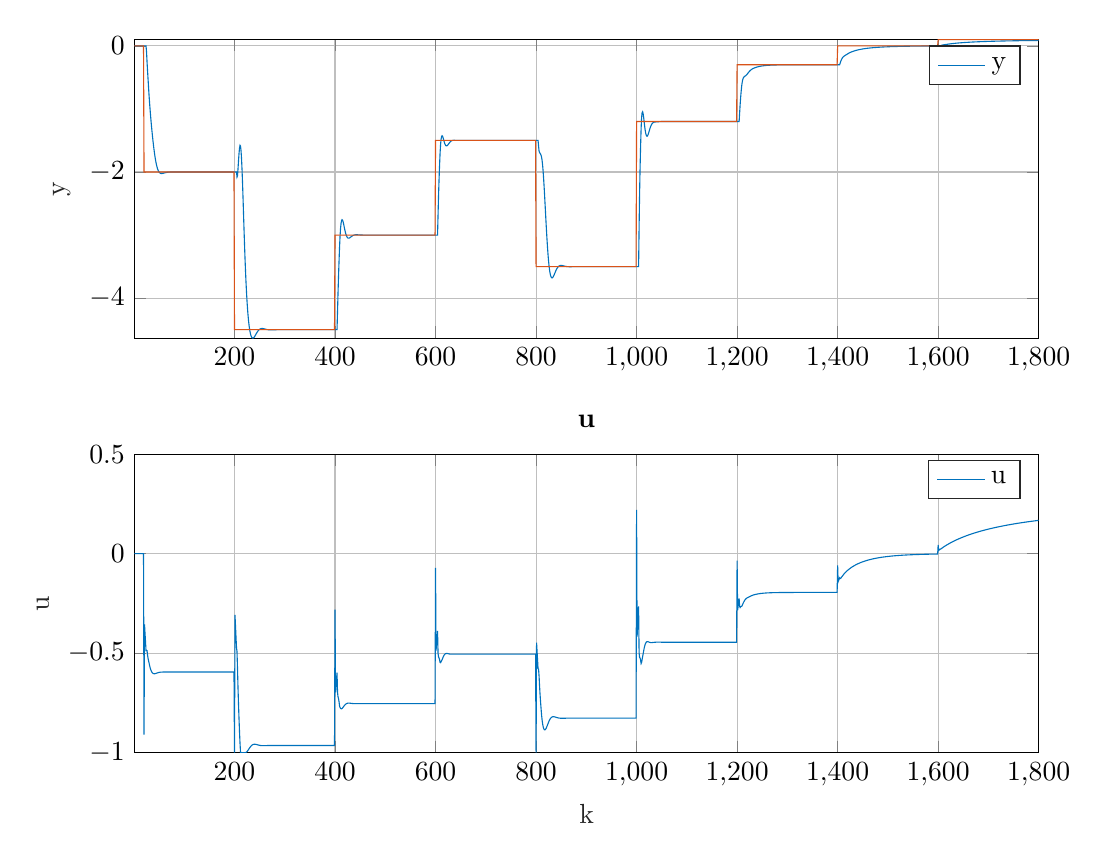
\begin{tikzpicture}

\begin{axis}[%
width=4.521in,
height=1.493in,
at={(0.758in,2.554in)},
scale only axis,
xmin=1,
xmax=1800,
ymin=-4.6335,
ymax=0.1,
ylabel style={font=\color{white!15!black}},
ylabel={y},
axis background/.style={fill=white},
xmajorgrids,
ymajorgrids,
legend style={legend cell align=left, align=left, draw=white!15!black}
]
\addplot [color=mycolor1]
  table[row sep=crcr]{%
1	0\\
2	0\\
3	0\\
4	0\\
5	0\\
6	0\\
7	0\\
8	0\\
9	0\\
10	0\\
11	0\\
12	0\\
13	0\\
14	0\\
15	0\\
16	0\\
17	0\\
18	0\\
19	0\\
20	0\\
21	0\\
22	0\\
23	0\\
24	0\\
25	-0.098378\\
26	-0.25368\\
27	-0.39312\\
28	-0.52557\\
29	-0.65731\\
30	-0.78382\\
31	-0.89914\\
32	-1.0051\\
33	-1.1044\\
34	-1.1976\\
35	-1.2852\\
36	-1.3679\\
37	-1.4461\\
38	-1.5199\\
39	-1.589\\
40	-1.6533\\
41	-1.7125\\
42	-1.7662\\
43	-1.8144\\
44	-1.8568\\
45	-1.8936\\
46	-1.9249\\
47	-1.951\\
48	-1.9721\\
49	-1.9889\\
50	-2.0016\\
51	-2.011\\
52	-2.0174\\
53	-2.0215\\
54	-2.0236\\
55	-2.0242\\
56	-2.0237\\
57	-2.0225\\
58	-2.0207\\
59	-2.0186\\
60	-2.0164\\
61	-2.0142\\
62	-2.0121\\
63	-2.0102\\
64	-2.0085\\
65	-2.0069\\
66	-2.0056\\
67	-2.0044\\
68	-2.0034\\
69	-2.0026\\
70	-2.002\\
71	-2.0014\\
72	-2.001\\
73	-2.0006\\
74	-2.0004\\
75	-2.0002\\
76	-2\\
77	-1.9999\\
78	-1.9998\\
79	-1.9998\\
80	-1.9997\\
81	-1.9997\\
82	-1.9997\\
83	-1.9997\\
84	-1.9997\\
85	-1.9997\\
86	-1.9998\\
87	-1.9998\\
88	-1.9998\\
89	-1.9998\\
90	-1.9999\\
91	-1.9999\\
92	-1.9999\\
93	-1.9999\\
94	-1.9999\\
95	-1.9999\\
96	-2\\
97	-2\\
98	-2\\
99	-2\\
100	-2\\
101	-2\\
102	-2\\
103	-2\\
104	-2\\
105	-2\\
106	-2\\
107	-2\\
108	-2\\
109	-2\\
110	-2\\
111	-2\\
112	-2\\
113	-2\\
114	-2\\
115	-2\\
116	-2\\
117	-2\\
118	-2\\
119	-2\\
120	-2\\
121	-2\\
122	-2\\
123	-2\\
124	-2\\
125	-2\\
126	-2\\
127	-2\\
128	-2\\
129	-2\\
130	-2\\
131	-2\\
132	-2\\
133	-2\\
134	-2\\
135	-2\\
136	-2\\
137	-2\\
138	-2\\
139	-2\\
140	-2\\
141	-2\\
142	-2\\
143	-2\\
144	-2\\
145	-2\\
146	-2\\
147	-2\\
148	-2\\
149	-2\\
150	-2\\
151	-2\\
152	-2\\
153	-2\\
154	-2\\
155	-2\\
156	-2\\
157	-2\\
158	-2\\
159	-2\\
160	-2\\
161	-2\\
162	-2\\
163	-2\\
164	-2\\
165	-2\\
166	-2\\
167	-2\\
168	-2\\
169	-2\\
170	-2\\
171	-2\\
172	-2\\
173	-2\\
174	-2\\
175	-2\\
176	-2\\
177	-2\\
178	-2\\
179	-2\\
180	-2\\
181	-2\\
182	-2\\
183	-2\\
184	-2\\
185	-2\\
186	-2\\
187	-2\\
188	-2\\
189	-2\\
190	-2\\
191	-2\\
192	-2\\
193	-2\\
194	-2\\
195	-2\\
196	-2\\
197	-2\\
198	-2\\
199	-2\\
200	-2\\
201	-2\\
202	-2\\
203	-2\\
204	-2\\
205	-2.0801\\
206	-2.0594\\
207	-1.9505\\
208	-1.8212\\
209	-1.7083\\
210	-1.6218\\
211	-1.578\\
212	-1.5904\\
213	-1.6617\\
214	-1.7873\\
215	-1.9604\\
216	-2.1727\\
217	-2.4144\\
218	-2.6692\\
219	-2.9216\\
220	-3.1617\\
221	-3.3836\\
222	-3.5845\\
223	-3.7634\\
224	-3.9207\\
225	-4.0574\\
226	-4.1752\\
227	-4.2758\\
228	-4.3608\\
229	-4.4317\\
230	-4.4898\\
231	-4.5363\\
232	-4.5724\\
233	-4.5992\\
234	-4.6177\\
235	-4.6288\\
236	-4.6335\\
237	-4.6329\\
238	-4.6279\\
239	-4.6195\\
240	-4.6084\\
241	-4.5957\\
242	-4.5819\\
243	-4.5677\\
244	-4.5538\\
245	-4.5405\\
246	-4.5283\\
247	-4.5174\\
248	-4.5078\\
249	-4.4999\\
250	-4.4934\\
251	-4.4884\\
252	-4.4849\\
253	-4.4826\\
254	-4.4814\\
255	-4.4811\\
256	-4.4817\\
257	-4.4828\\
258	-4.4844\\
259	-4.4863\\
260	-4.4883\\
261	-4.4904\\
262	-4.4925\\
263	-4.4944\\
264	-4.4962\\
265	-4.4978\\
266	-4.4992\\
267	-4.5003\\
268	-4.5012\\
269	-4.5019\\
270	-4.5024\\
271	-4.5027\\
272	-4.5028\\
273	-4.5028\\
274	-4.5027\\
275	-4.5025\\
276	-4.5022\\
277	-4.5019\\
278	-4.5016\\
279	-4.5013\\
280	-4.501\\
281	-4.5007\\
282	-4.5005\\
283	-4.5002\\
284	-4.5\\
285	-4.4999\\
286	-4.4998\\
287	-4.4997\\
288	-4.4996\\
289	-4.4996\\
290	-4.4996\\
291	-4.4996\\
292	-4.4996\\
293	-4.4996\\
294	-4.4997\\
295	-4.4997\\
296	-4.4998\\
297	-4.4998\\
298	-4.4999\\
299	-4.4999\\
300	-4.4999\\
301	-4.5\\
302	-4.5\\
303	-4.5\\
304	-4.5\\
305	-4.5001\\
306	-4.5001\\
307	-4.5001\\
308	-4.5001\\
309	-4.5001\\
310	-4.5001\\
311	-4.5001\\
312	-4.5\\
313	-4.5\\
314	-4.5\\
315	-4.5\\
316	-4.5\\
317	-4.5\\
318	-4.5\\
319	-4.5\\
320	-4.5\\
321	-4.5\\
322	-4.5\\
323	-4.5\\
324	-4.5\\
325	-4.5\\
326	-4.5\\
327	-4.5\\
328	-4.5\\
329	-4.5\\
330	-4.5\\
331	-4.5\\
332	-4.5\\
333	-4.5\\
334	-4.5\\
335	-4.5\\
336	-4.5\\
337	-4.5\\
338	-4.5\\
339	-4.5\\
340	-4.5\\
341	-4.5\\
342	-4.5\\
343	-4.5\\
344	-4.5\\
345	-4.5\\
346	-4.5\\
347	-4.5\\
348	-4.5\\
349	-4.5\\
350	-4.5\\
351	-4.5\\
352	-4.5\\
353	-4.5\\
354	-4.5\\
355	-4.5\\
356	-4.5\\
357	-4.5\\
358	-4.5\\
359	-4.5\\
360	-4.5\\
361	-4.5\\
362	-4.5\\
363	-4.5\\
364	-4.5\\
365	-4.5\\
366	-4.5\\
367	-4.5\\
368	-4.5\\
369	-4.5\\
370	-4.5\\
371	-4.5\\
372	-4.5\\
373	-4.5\\
374	-4.5\\
375	-4.5\\
376	-4.5\\
377	-4.5\\
378	-4.5\\
379	-4.5\\
380	-4.5\\
381	-4.5\\
382	-4.5\\
383	-4.5\\
384	-4.5\\
385	-4.5\\
386	-4.5\\
387	-4.5\\
388	-4.5\\
389	-4.5\\
390	-4.5\\
391	-4.5\\
392	-4.5\\
393	-4.5\\
394	-4.5\\
395	-4.5\\
396	-4.5\\
397	-4.5\\
398	-4.5\\
399	-4.5\\
400	-4.5\\
401	-4.5\\
402	-4.5\\
403	-4.5\\
404	-4.5\\
405	-4.2111\\
406	-3.9122\\
407	-3.6513\\
408	-3.4154\\
409	-3.1953\\
410	-3.0205\\
411	-2.8973\\
412	-2.8167\\
413	-2.7711\\
414	-2.7555\\
415	-2.7635\\
416	-2.7875\\
417	-2.8211\\
418	-2.8594\\
419	-2.8985\\
420	-2.9354\\
421	-2.968\\
422	-2.9952\\
423	-3.0166\\
424	-3.0322\\
425	-3.0424\\
426	-3.0479\\
427	-3.0495\\
428	-3.0481\\
429	-3.0444\\
430	-3.0392\\
431	-3.0333\\
432	-3.0271\\
433	-3.021\\
434	-3.0153\\
435	-3.0103\\
436	-3.006\\
437	-3.0025\\
438	-2.9998\\
439	-2.9977\\
440	-2.9964\\
441	-2.9955\\
442	-2.9951\\
443	-2.9951\\
444	-2.9953\\
445	-2.9957\\
446	-2.9962\\
447	-2.9967\\
448	-2.9973\\
449	-2.9978\\
450	-2.9983\\
451	-2.9988\\
452	-2.9992\\
453	-2.9995\\
454	-2.9997\\
455	-2.9999\\
456	-3.0001\\
457	-3.0002\\
458	-3.0003\\
459	-3.0003\\
460	-3.0003\\
461	-3.0003\\
462	-3.0003\\
463	-3.0003\\
464	-3.0002\\
465	-3.0002\\
466	-3.0002\\
467	-3.0001\\
468	-3.0001\\
469	-3.0001\\
470	-3.0001\\
471	-3\\
472	-3\\
473	-3\\
474	-3\\
475	-3\\
476	-3\\
477	-3\\
478	-3\\
479	-3\\
480	-3\\
481	-3\\
482	-3\\
483	-3\\
484	-3\\
485	-3\\
486	-3\\
487	-3\\
488	-3\\
489	-3\\
490	-3\\
491	-3\\
492	-3\\
493	-3\\
494	-3\\
495	-3\\
496	-3\\
497	-3\\
498	-3\\
499	-3\\
500	-3\\
501	-3\\
502	-3\\
503	-3\\
504	-3\\
505	-3\\
506	-3\\
507	-3\\
508	-3\\
509	-3\\
510	-3\\
511	-3\\
512	-3\\
513	-3\\
514	-3\\
515	-3\\
516	-3\\
517	-3\\
518	-3\\
519	-3\\
520	-3\\
521	-3\\
522	-3\\
523	-3\\
524	-3\\
525	-3\\
526	-3\\
527	-3\\
528	-3\\
529	-3\\
530	-3\\
531	-3\\
532	-3\\
533	-3\\
534	-3\\
535	-3\\
536	-3\\
537	-3\\
538	-3\\
539	-3\\
540	-3\\
541	-3\\
542	-3\\
543	-3\\
544	-3\\
545	-3\\
546	-3\\
547	-3\\
548	-3\\
549	-3\\
550	-3\\
551	-3\\
552	-3\\
553	-3\\
554	-3\\
555	-3\\
556	-3\\
557	-3\\
558	-3\\
559	-3\\
560	-3\\
561	-3\\
562	-3\\
563	-3\\
564	-3\\
565	-3\\
566	-3\\
567	-3\\
568	-3\\
569	-3\\
570	-3\\
571	-3\\
572	-3\\
573	-3\\
574	-3\\
575	-3\\
576	-3\\
577	-3\\
578	-3\\
579	-3\\
580	-3\\
581	-3\\
582	-3\\
583	-3\\
584	-3\\
585	-3\\
586	-3\\
587	-3\\
588	-3\\
589	-3\\
590	-3\\
591	-3\\
592	-3\\
593	-3\\
594	-3\\
595	-3\\
596	-3\\
597	-3\\
598	-3\\
599	-3\\
600	-3\\
601	-3\\
602	-3\\
603	-3\\
604	-3\\
605	-2.6784\\
606	-2.37\\
607	-2.1158\\
608	-1.8985\\
609	-1.706\\
610	-1.5671\\
611	-1.4829\\
612	-1.4393\\
613	-1.4251\\
614	-1.4334\\
615	-1.4562\\
616	-1.4855\\
617	-1.5153\\
618	-1.542\\
619	-1.5631\\
620	-1.5775\\
621	-1.5851\\
622	-1.5865\\
623	-1.5829\\
624	-1.5755\\
625	-1.5658\\
626	-1.5549\\
627	-1.5439\\
628	-1.5334\\
629	-1.5242\\
630	-1.5164\\
631	-1.5101\\
632	-1.5054\\
633	-1.502\\
634	-1.4998\\
635	-1.4985\\
636	-1.4979\\
637	-1.4977\\
638	-1.4979\\
639	-1.4982\\
640	-1.4986\\
641	-1.499\\
642	-1.4993\\
643	-1.4995\\
644	-1.4997\\
645	-1.4997\\
646	-1.4998\\
647	-1.4998\\
648	-1.4997\\
649	-1.4997\\
650	-1.4996\\
651	-1.4996\\
652	-1.4996\\
653	-1.4996\\
654	-1.4996\\
655	-1.4996\\
656	-1.4997\\
657	-1.4997\\
658	-1.4997\\
659	-1.4998\\
660	-1.4998\\
661	-1.4999\\
662	-1.4999\\
663	-1.4999\\
664	-1.4999\\
665	-1.5\\
666	-1.5\\
667	-1.5\\
668	-1.5\\
669	-1.5\\
670	-1.5\\
671	-1.5\\
672	-1.5\\
673	-1.5\\
674	-1.5\\
675	-1.5\\
676	-1.5\\
677	-1.5\\
678	-1.5\\
679	-1.5\\
680	-1.5\\
681	-1.5\\
682	-1.5\\
683	-1.5\\
684	-1.5\\
685	-1.5\\
686	-1.5\\
687	-1.5\\
688	-1.5\\
689	-1.5\\
690	-1.5\\
691	-1.5\\
692	-1.5\\
693	-1.5\\
694	-1.5\\
695	-1.5\\
696	-1.5\\
697	-1.5\\
698	-1.5\\
699	-1.5\\
700	-1.5\\
701	-1.5\\
702	-1.5\\
703	-1.5\\
704	-1.5\\
705	-1.5\\
706	-1.5\\
707	-1.5\\
708	-1.5\\
709	-1.5\\
710	-1.5\\
711	-1.5\\
712	-1.5\\
713	-1.5\\
714	-1.5\\
715	-1.5\\
716	-1.5\\
717	-1.5\\
718	-1.5\\
719	-1.5\\
720	-1.5\\
721	-1.5\\
722	-1.5\\
723	-1.5\\
724	-1.5\\
725	-1.5\\
726	-1.5\\
727	-1.5\\
728	-1.5\\
729	-1.5\\
730	-1.5\\
731	-1.5\\
732	-1.5\\
733	-1.5\\
734	-1.5\\
735	-1.5\\
736	-1.5\\
737	-1.5\\
738	-1.5\\
739	-1.5\\
740	-1.5\\
741	-1.5\\
742	-1.5\\
743	-1.5\\
744	-1.5\\
745	-1.5\\
746	-1.5\\
747	-1.5\\
748	-1.5\\
749	-1.5\\
750	-1.5\\
751	-1.5\\
752	-1.5\\
753	-1.5\\
754	-1.5\\
755	-1.5\\
756	-1.5\\
757	-1.5\\
758	-1.5\\
759	-1.5\\
760	-1.5\\
761	-1.5\\
762	-1.5\\
763	-1.5\\
764	-1.5\\
765	-1.5\\
766	-1.5\\
767	-1.5\\
768	-1.5\\
769	-1.5\\
770	-1.5\\
771	-1.5\\
772	-1.5\\
773	-1.5\\
774	-1.5\\
775	-1.5\\
776	-1.5\\
777	-1.5\\
778	-1.5\\
779	-1.5\\
780	-1.5\\
781	-1.5\\
782	-1.5\\
783	-1.5\\
784	-1.5\\
785	-1.5\\
786	-1.5\\
787	-1.5\\
788	-1.5\\
789	-1.5\\
790	-1.5\\
791	-1.5\\
792	-1.5\\
793	-1.5\\
794	-1.5\\
795	-1.5\\
796	-1.5\\
797	-1.5\\
798	-1.5\\
799	-1.5\\
800	-1.5\\
801	-1.5\\
802	-1.5\\
803	-1.5\\
804	-1.5\\
805	-1.593\\
806	-1.6684\\
807	-1.6941\\
808	-1.7035\\
809	-1.717\\
810	-1.7365\\
811	-1.7668\\
812	-1.8165\\
813	-1.8893\\
814	-1.9843\\
815	-2.0988\\
816	-2.2295\\
817	-2.3721\\
818	-2.5216\\
819	-2.6732\\
820	-2.8226\\
821	-2.9658\\
822	-3.0995\\
823	-3.2213\\
824	-3.3292\\
825	-3.4223\\
826	-3.4999\\
827	-3.5623\\
828	-3.6101\\
829	-3.6442\\
830	-3.666\\
831	-3.6771\\
832	-3.6791\\
833	-3.6737\\
834	-3.6627\\
835	-3.6476\\
836	-3.6298\\
837	-3.6107\\
838	-3.5912\\
839	-3.5723\\
840	-3.5545\\
841	-3.5385\\
842	-3.5244\\
843	-3.5124\\
844	-3.5026\\
845	-3.4949\\
846	-3.4892\\
847	-3.4852\\
848	-3.4827\\
849	-3.4815\\
850	-3.4813\\
851	-3.482\\
852	-3.4833\\
853	-3.4849\\
854	-3.4869\\
855	-3.4889\\
856	-3.4909\\
857	-3.4929\\
858	-3.4947\\
859	-3.4963\\
860	-3.4977\\
861	-3.4988\\
862	-3.4998\\
863	-3.5005\\
864	-3.5011\\
865	-3.5014\\
866	-3.5017\\
867	-3.5018\\
868	-3.5018\\
869	-3.5017\\
870	-3.5016\\
871	-3.5014\\
872	-3.5012\\
873	-3.5011\\
874	-3.5009\\
875	-3.5007\\
876	-3.5005\\
877	-3.5004\\
878	-3.5002\\
879	-3.5001\\
880	-3.5\\
881	-3.5\\
882	-3.4999\\
883	-3.4999\\
884	-3.4998\\
885	-3.4998\\
886	-3.4998\\
887	-3.4998\\
888	-3.4999\\
889	-3.4999\\
890	-3.4999\\
891	-3.4999\\
892	-3.4999\\
893	-3.4999\\
894	-3.5\\
895	-3.5\\
896	-3.5\\
897	-3.5\\
898	-3.5\\
899	-3.5\\
900	-3.5\\
901	-3.5\\
902	-3.5\\
903	-3.5\\
904	-3.5\\
905	-3.5\\
906	-3.5\\
907	-3.5\\
908	-3.5\\
909	-3.5\\
910	-3.5\\
911	-3.5\\
912	-3.5\\
913	-3.5\\
914	-3.5\\
915	-3.5\\
916	-3.5\\
917	-3.5\\
918	-3.5\\
919	-3.5\\
920	-3.5\\
921	-3.5\\
922	-3.5\\
923	-3.5\\
924	-3.5\\
925	-3.5\\
926	-3.5\\
927	-3.5\\
928	-3.5\\
929	-3.5\\
930	-3.5\\
931	-3.5\\
932	-3.5\\
933	-3.5\\
934	-3.5\\
935	-3.5\\
936	-3.5\\
937	-3.5\\
938	-3.5\\
939	-3.5\\
940	-3.5\\
941	-3.5\\
942	-3.5\\
943	-3.5\\
944	-3.5\\
945	-3.5\\
946	-3.5\\
947	-3.5\\
948	-3.5\\
949	-3.5\\
950	-3.5\\
951	-3.5\\
952	-3.5\\
953	-3.5\\
954	-3.5\\
955	-3.5\\
956	-3.5\\
957	-3.5\\
958	-3.5\\
959	-3.5\\
960	-3.5\\
961	-3.5\\
962	-3.5\\
963	-3.5\\
964	-3.5\\
965	-3.5\\
966	-3.5\\
967	-3.5\\
968	-3.5\\
969	-3.5\\
970	-3.5\\
971	-3.5\\
972	-3.5\\
973	-3.5\\
974	-3.5\\
975	-3.5\\
976	-3.5\\
977	-3.5\\
978	-3.5\\
979	-3.5\\
980	-3.5\\
981	-3.5\\
982	-3.5\\
983	-3.5\\
984	-3.5\\
985	-3.5\\
986	-3.5\\
987	-3.5\\
988	-3.5\\
989	-3.5\\
990	-3.5\\
991	-3.5\\
992	-3.5\\
993	-3.5\\
994	-3.5\\
995	-3.5\\
996	-3.5\\
997	-3.5\\
998	-3.5\\
999	-3.5\\
1000	-3.5\\
1001	-3.5\\
1002	-3.5\\
1003	-3.5\\
1004	-3.5\\
1005	-2.8781\\
1006	-2.3361\\
1007	-1.9185\\
1008	-1.5862\\
1009	-1.312\\
1010	-1.138\\
1011	-1.0595\\
1012	-1.0456\\
1013	-1.0737\\
1014	-1.1298\\
1015	-1.1999\\
1016	-1.2704\\
1017	-1.3323\\
1018	-1.3808\\
1019	-1.4136\\
1020	-1.4304\\
1021	-1.4326\\
1022	-1.4228\\
1023	-1.4044\\
1024	-1.3804\\
1025	-1.3538\\
1026	-1.3269\\
1027	-1.3017\\
1028	-1.2792\\
1029	-1.2602\\
1030	-1.2448\\
1031	-1.2328\\
1032	-1.2239\\
1033	-1.2176\\
1034	-1.2133\\
1035	-1.2105\\
1036	-1.2087\\
1037	-1.2076\\
1038	-1.2069\\
1039	-1.2063\\
1040	-1.2057\\
1041	-1.2051\\
1042	-1.2045\\
1043	-1.2038\\
1044	-1.2031\\
1045	-1.2024\\
1046	-1.2018\\
1047	-1.2012\\
1048	-1.2007\\
1049	-1.2003\\
1050	-1.2\\
1051	-1.1998\\
1052	-1.1997\\
1053	-1.1996\\
1054	-1.1995\\
1055	-1.1995\\
1056	-1.1995\\
1057	-1.1996\\
1058	-1.1996\\
1059	-1.1997\\
1060	-1.1997\\
1061	-1.1998\\
1062	-1.1998\\
1063	-1.1998\\
1064	-1.1999\\
1065	-1.1999\\
1066	-1.1999\\
1067	-1.1999\\
1068	-1.1999\\
1069	-1.1999\\
1070	-1.1999\\
1071	-1.1999\\
1072	-1.1999\\
1073	-1.2\\
1074	-1.2\\
1075	-1.2\\
1076	-1.2\\
1077	-1.2\\
1078	-1.2\\
1079	-1.2\\
1080	-1.2\\
1081	-1.2\\
1082	-1.2\\
1083	-1.2\\
1084	-1.2\\
1085	-1.2\\
1086	-1.2\\
1087	-1.2\\
1088	-1.2\\
1089	-1.2\\
1090	-1.2\\
1091	-1.2\\
1092	-1.2\\
1093	-1.2\\
1094	-1.2\\
1095	-1.2\\
1096	-1.2\\
1097	-1.2\\
1098	-1.2\\
1099	-1.2\\
1100	-1.2\\
1101	-1.2\\
1102	-1.2\\
1103	-1.2\\
1104	-1.2\\
1105	-1.2\\
1106	-1.2\\
1107	-1.2\\
1108	-1.2\\
1109	-1.2\\
1110	-1.2\\
1111	-1.2\\
1112	-1.2\\
1113	-1.2\\
1114	-1.2\\
1115	-1.2\\
1116	-1.2\\
1117	-1.2\\
1118	-1.2\\
1119	-1.2\\
1120	-1.2\\
1121	-1.2\\
1122	-1.2\\
1123	-1.2\\
1124	-1.2\\
1125	-1.2\\
1126	-1.2\\
1127	-1.2\\
1128	-1.2\\
1129	-1.2\\
1130	-1.2\\
1131	-1.2\\
1132	-1.2\\
1133	-1.2\\
1134	-1.2\\
1135	-1.2\\
1136	-1.2\\
1137	-1.2\\
1138	-1.2\\
1139	-1.2\\
1140	-1.2\\
1141	-1.2\\
1142	-1.2\\
1143	-1.2\\
1144	-1.2\\
1145	-1.2\\
1146	-1.2\\
1147	-1.2\\
1148	-1.2\\
1149	-1.2\\
1150	-1.2\\
1151	-1.2\\
1152	-1.2\\
1153	-1.2\\
1154	-1.2\\
1155	-1.2\\
1156	-1.2\\
1157	-1.2\\
1158	-1.2\\
1159	-1.2\\
1160	-1.2\\
1161	-1.2\\
1162	-1.2\\
1163	-1.2\\
1164	-1.2\\
1165	-1.2\\
1166	-1.2\\
1167	-1.2\\
1168	-1.2\\
1169	-1.2\\
1170	-1.2\\
1171	-1.2\\
1172	-1.2\\
1173	-1.2\\
1174	-1.2\\
1175	-1.2\\
1176	-1.2\\
1177	-1.2\\
1178	-1.2\\
1179	-1.2\\
1180	-1.2\\
1181	-1.2\\
1182	-1.2\\
1183	-1.2\\
1184	-1.2\\
1185	-1.2\\
1186	-1.2\\
1187	-1.2\\
1188	-1.2\\
1189	-1.2\\
1190	-1.2\\
1191	-1.2\\
1192	-1.2\\
1193	-1.2\\
1194	-1.2\\
1195	-1.2\\
1196	-1.2\\
1197	-1.2\\
1198	-1.2\\
1199	-1.2\\
1200	-1.2\\
1201	-1.2\\
1202	-1.2\\
1203	-1.2\\
1204	-1.2\\
1205	-1.0699\\
1206	-0.9347\\
1207	-0.82309\\
1208	-0.72852\\
1209	-0.64625\\
1210	-0.58455\\
1211	-0.5436\\
1212	-0.51734\\
1213	-0.5008\\
1214	-0.49082\\
1215	-0.4845\\
1216	-0.47924\\
1217	-0.47348\\
1218	-0.46657\\
1219	-0.45837\\
1220	-0.44907\\
1221	-0.43906\\
1222	-0.4288\\
1223	-0.41874\\
1224	-0.40918\\
1225	-0.40036\\
1226	-0.39236\\
1227	-0.38522\\
1228	-0.37887\\
1229	-0.37324\\
1230	-0.36821\\
1231	-0.36369\\
1232	-0.35958\\
1233	-0.3558\\
1234	-0.3523\\
1235	-0.34904\\
1236	-0.34597\\
1237	-0.3431\\
1238	-0.3404\\
1239	-0.33786\\
1240	-0.33549\\
1241	-0.33326\\
1242	-0.33118\\
1243	-0.32924\\
1244	-0.32743\\
1245	-0.32574\\
1246	-0.32417\\
1247	-0.3227\\
1248	-0.32132\\
1249	-0.32003\\
1250	-0.31883\\
1251	-0.3177\\
1252	-0.31664\\
1253	-0.31564\\
1254	-0.31471\\
1255	-0.31383\\
1256	-0.31301\\
1257	-0.31224\\
1258	-0.31151\\
1259	-0.31083\\
1260	-0.31019\\
1261	-0.30959\\
1262	-0.30903\\
1263	-0.30849\\
1264	-0.308\\
1265	-0.30753\\
1266	-0.30709\\
1267	-0.30667\\
1268	-0.30628\\
1269	-0.30591\\
1270	-0.30557\\
1271	-0.30524\\
1272	-0.30494\\
1273	-0.30465\\
1274	-0.30438\\
1275	-0.30412\\
1276	-0.30388\\
1277	-0.30366\\
1278	-0.30344\\
1279	-0.30324\\
1280	-0.30306\\
1281	-0.30288\\
1282	-0.30271\\
1283	-0.30255\\
1284	-0.30241\\
1285	-0.30227\\
1286	-0.30214\\
1287	-0.30201\\
1288	-0.30189\\
1289	-0.30179\\
1290	-0.30168\\
1291	-0.30158\\
1292	-0.30149\\
1293	-0.30141\\
1294	-0.30132\\
1295	-0.30125\\
1296	-0.30118\\
1297	-0.30111\\
1298	-0.30104\\
1299	-0.30098\\
1300	-0.30093\\
1301	-0.30087\\
1302	-0.30082\\
1303	-0.30078\\
1304	-0.30073\\
1305	-0.30069\\
1306	-0.30065\\
1307	-0.30061\\
1308	-0.30058\\
1309	-0.30054\\
1310	-0.30051\\
1311	-0.30048\\
1312	-0.30045\\
1313	-0.30043\\
1314	-0.3004\\
1315	-0.30038\\
1316	-0.30036\\
1317	-0.30034\\
1318	-0.30032\\
1319	-0.3003\\
1320	-0.30028\\
1321	-0.30027\\
1322	-0.30025\\
1323	-0.30024\\
1324	-0.30022\\
1325	-0.30021\\
1326	-0.3002\\
1327	-0.30019\\
1328	-0.30018\\
1329	-0.30017\\
1330	-0.30016\\
1331	-0.30015\\
1332	-0.30014\\
1333	-0.30013\\
1334	-0.30012\\
1335	-0.30012\\
1336	-0.30011\\
1337	-0.3001\\
1338	-0.3001\\
1339	-0.30009\\
1340	-0.30009\\
1341	-0.30008\\
1342	-0.30008\\
1343	-0.30007\\
1344	-0.30007\\
1345	-0.30006\\
1346	-0.30006\\
1347	-0.30006\\
1348	-0.30005\\
1349	-0.30005\\
1350	-0.30005\\
1351	-0.30004\\
1352	-0.30004\\
1353	-0.30004\\
1354	-0.30004\\
1355	-0.30004\\
1356	-0.30003\\
1357	-0.30003\\
1358	-0.30003\\
1359	-0.30003\\
1360	-0.30003\\
1361	-0.30002\\
1362	-0.30002\\
1363	-0.30002\\
1364	-0.30002\\
1365	-0.30002\\
1366	-0.30002\\
1367	-0.30002\\
1368	-0.30002\\
1369	-0.30002\\
1370	-0.30001\\
1371	-0.30001\\
1372	-0.30001\\
1373	-0.30001\\
1374	-0.30001\\
1375	-0.30001\\
1376	-0.30001\\
1377	-0.30001\\
1378	-0.30001\\
1379	-0.30001\\
1380	-0.30001\\
1381	-0.30001\\
1382	-0.30001\\
1383	-0.30001\\
1384	-0.30001\\
1385	-0.30001\\
1386	-0.30001\\
1387	-0.30001\\
1388	-0.3\\
1389	-0.3\\
1390	-0.3\\
1391	-0.3\\
1392	-0.3\\
1393	-0.3\\
1394	-0.3\\
1395	-0.3\\
1396	-0.3\\
1397	-0.3\\
1398	-0.3\\
1399	-0.3\\
1400	-0.3\\
1401	-0.3\\
1402	-0.3\\
1403	-0.3\\
1404	-0.3\\
1405	-0.2777\\
1406	-0.25099\\
1407	-0.22962\\
1408	-0.21197\\
1409	-0.19682\\
1410	-0.18468\\
1411	-0.17556\\
1412	-0.16843\\
1413	-0.16241\\
1414	-0.15703\\
1415	-0.15197\\
1416	-0.14699\\
1417	-0.14201\\
1418	-0.13702\\
1419	-0.13207\\
1420	-0.12722\\
1421	-0.12252\\
1422	-0.11802\\
1423	-0.11374\\
1424	-0.10968\\
1425	-0.10584\\
1426	-0.10221\\
1427	-0.098772\\
1428	-0.095507\\
1429	-0.092401\\
1430	-0.089439\\
1431	-0.086609\\
1432	-0.0839\\
1433	-0.081305\\
1434	-0.078818\\
1435	-0.076431\\
1436	-0.07414\\
1437	-0.07194\\
1438	-0.069826\\
1439	-0.067794\\
1440	-0.06584\\
1441	-0.063961\\
1442	-0.062151\\
1443	-0.060408\\
1444	-0.058729\\
1445	-0.05711\\
1446	-0.055548\\
1447	-0.054041\\
1448	-0.052586\\
1449	-0.051181\\
1450	-0.049823\\
1451	-0.04851\\
1452	-0.047241\\
1453	-0.046014\\
1454	-0.044826\\
1455	-0.043676\\
1456	-0.042563\\
1457	-0.041484\\
1458	-0.040439\\
1459	-0.039427\\
1460	-0.038445\\
1461	-0.037493\\
1462	-0.03657\\
1463	-0.035674\\
1464	-0.034804\\
1465	-0.03396\\
1466	-0.03314\\
1467	-0.032344\\
1468	-0.031571\\
1469	-0.030819\\
1470	-0.030089\\
1471	-0.029379\\
1472	-0.028689\\
1473	-0.028018\\
1474	-0.027365\\
1475	-0.02673\\
1476	-0.026112\\
1477	-0.02551\\
1478	-0.024925\\
1479	-0.024355\\
1480	-0.0238\\
1481	-0.02326\\
1482	-0.022733\\
1483	-0.02222\\
1484	-0.021721\\
1485	-0.021234\\
1486	-0.02076\\
1487	-0.020297\\
1488	-0.019846\\
1489	-0.019407\\
1490	-0.018978\\
1491	-0.01856\\
1492	-0.018153\\
1493	-0.017755\\
1494	-0.017367\\
1495	-0.016988\\
1496	-0.016619\\
1497	-0.016259\\
1498	-0.015907\\
1499	-0.015564\\
1500	-0.015228\\
1501	-0.014901\\
1502	-0.014582\\
1503	-0.01427\\
1504	-0.013965\\
1505	-0.013667\\
1506	-0.013377\\
1507	-0.013093\\
1508	-0.012815\\
1509	-0.012544\\
1510	-0.01228\\
1511	-0.012021\\
1512	-0.011768\\
1513	-0.011521\\
1514	-0.01128\\
1515	-0.011044\\
1516	-0.010813\\
1517	-0.010587\\
1518	-0.010367\\
1519	-0.010151\\
1520	-0.0099404\\
1521	-0.0097343\\
1522	-0.0095328\\
1523	-0.0093357\\
1524	-0.009143\\
1525	-0.0089545\\
1526	-0.0087701\\
1527	-0.0085897\\
1528	-0.0084133\\
1529	-0.0082407\\
1530	-0.0080719\\
1531	-0.0079067\\
1532	-0.0077451\\
1533	-0.0075869\\
1534	-0.0074322\\
1535	-0.0072808\\
1536	-0.0071326\\
1537	-0.0069876\\
1538	-0.0068457\\
1539	-0.0067068\\
1540	-0.0065709\\
1541	-0.0064378\\
1542	-0.0063076\\
1543	-0.0061801\\
1544	-0.0060553\\
1545	-0.0059332\\
1546	-0.0058136\\
1547	-0.0056965\\
1548	-0.0055819\\
1549	-0.0054696\\
1550	-0.0053597\\
1551	-0.0052521\\
1552	-0.0051468\\
1553	-0.0050436\\
1554	-0.0049426\\
1555	-0.0048437\\
1556	-0.0047468\\
1557	-0.004652\\
1558	-0.0045591\\
1559	-0.0044681\\
1560	-0.0043789\\
1561	-0.0042917\\
1562	-0.0042062\\
1563	-0.0041224\\
1564	-0.0040404\\
1565	-0.0039601\\
1566	-0.0038814\\
1567	-0.0038043\\
1568	-0.0037288\\
1569	-0.0036548\\
1570	-0.0035823\\
1571	-0.0035114\\
1572	-0.0034418\\
1573	-0.0033737\\
1574	-0.0033069\\
1575	-0.0032415\\
1576	-0.0031774\\
1577	-0.0031146\\
1578	-0.0030531\\
1579	-0.0029929\\
1580	-0.0029338\\
1581	-0.0028759\\
1582	-0.0028192\\
1583	-0.0027637\\
1584	-0.0027092\\
1585	-0.0026559\\
1586	-0.0026036\\
1587	-0.0025524\\
1588	-0.0025022\\
1589	-0.002453\\
1590	-0.0024048\\
1591	-0.0023575\\
1592	-0.0023112\\
1593	-0.0022659\\
1594	-0.0022214\\
1595	-0.0021778\\
1596	-0.0021351\\
1597	-0.0020932\\
1598	-0.0020522\\
1599	-0.002012\\
1600	-0.0019726\\
1601	-0.0019339\\
1602	-0.0018961\\
1603	-0.001859\\
1604	-0.0018226\\
1605	0.0010104\\
1606	0.0054261\\
1607	0.0085557\\
1608	0.010921\\
1609	0.012857\\
1610	0.014497\\
1611	0.015877\\
1612	0.017104\\
1613	0.018289\\
1614	0.019473\\
1615	0.020666\\
1616	0.021868\\
1617	0.02307\\
1618	0.024265\\
1619	0.025443\\
1620	0.026598\\
1621	0.027724\\
1622	0.028822\\
1623	0.02989\\
1624	0.03093\\
1625	0.031942\\
1626	0.032928\\
1627	0.033889\\
1628	0.034826\\
1629	0.035741\\
1630	0.036634\\
1631	0.037506\\
1632	0.038358\\
1633	0.03919\\
1634	0.040004\\
1635	0.040799\\
1636	0.041576\\
1637	0.042336\\
1638	0.043079\\
1639	0.043806\\
1640	0.044518\\
1641	0.045214\\
1642	0.045896\\
1643	0.046563\\
1644	0.047217\\
1645	0.047858\\
1646	0.048485\\
1647	0.0491\\
1648	0.049703\\
1649	0.050293\\
1650	0.050873\\
1651	0.051441\\
1652	0.051998\\
1653	0.052544\\
1654	0.05308\\
1655	0.053607\\
1656	0.054123\\
1657	0.05463\\
1658	0.055128\\
1659	0.055617\\
1660	0.056097\\
1661	0.056569\\
1662	0.057032\\
1663	0.057487\\
1664	0.057934\\
1665	0.058374\\
1666	0.058806\\
1667	0.059231\\
1668	0.059649\\
1669	0.060059\\
1670	0.060463\\
1671	0.060861\\
1672	0.061251\\
1673	0.061636\\
1674	0.062014\\
1675	0.062387\\
1676	0.062753\\
1677	0.063114\\
1678	0.063469\\
1679	0.063819\\
1680	0.064163\\
1681	0.064502\\
1682	0.064836\\
1683	0.065165\\
1684	0.065489\\
1685	0.065808\\
1686	0.066122\\
1687	0.066432\\
1688	0.066738\\
1689	0.067039\\
1690	0.067335\\
1691	0.067628\\
1692	0.067916\\
1693	0.0682\\
1694	0.068481\\
1695	0.068757\\
1696	0.069029\\
1697	0.069298\\
1698	0.069563\\
1699	0.069825\\
1700	0.070083\\
1701	0.070338\\
1702	0.070589\\
1703	0.070837\\
1704	0.071082\\
1705	0.071323\\
1706	0.071561\\
1707	0.071797\\
1708	0.072029\\
1709	0.072258\\
1710	0.072484\\
1711	0.072708\\
1712	0.072929\\
1713	0.073147\\
1714	0.073362\\
1715	0.073575\\
1716	0.073785\\
1717	0.073992\\
1718	0.074197\\
1719	0.074399\\
1720	0.074599\\
1721	0.074797\\
1722	0.074992\\
1723	0.075185\\
1724	0.075376\\
1725	0.075565\\
1726	0.075751\\
1727	0.075935\\
1728	0.076117\\
1729	0.076297\\
1730	0.076475\\
1731	0.076651\\
1732	0.076825\\
1733	0.076997\\
1734	0.077167\\
1735	0.077335\\
1736	0.077501\\
1737	0.077666\\
1738	0.077828\\
1739	0.077989\\
1740	0.078149\\
1741	0.078306\\
1742	0.078462\\
1743	0.078616\\
1744	0.078768\\
1745	0.078919\\
1746	0.079068\\
1747	0.079216\\
1748	0.079362\\
1749	0.079507\\
1750	0.07965\\
1751	0.079792\\
1752	0.079932\\
1753	0.080071\\
1754	0.080208\\
1755	0.080344\\
1756	0.080479\\
1757	0.080612\\
1758	0.080744\\
1759	0.080874\\
1760	0.081004\\
1761	0.081132\\
1762	0.081259\\
1763	0.081384\\
1764	0.081508\\
1765	0.081632\\
1766	0.081753\\
1767	0.081874\\
1768	0.081994\\
1769	0.082112\\
1770	0.08223\\
1771	0.082346\\
1772	0.082461\\
1773	0.082575\\
1774	0.082688\\
1775	0.0828\\
1776	0.082911\\
1777	0.083021\\
1778	0.08313\\
1779	0.083238\\
1780	0.083344\\
1781	0.08345\\
1782	0.083555\\
1783	0.083659\\
1784	0.083762\\
1785	0.083865\\
1786	0.083966\\
1787	0.084066\\
1788	0.084166\\
1789	0.084264\\
1790	0.084362\\
1791	0.084459\\
1792	0.084555\\
1793	0.08465\\
1794	0.084744\\
1795	0.084838\\
1796	0.08493\\
1797	0.085022\\
1798	0.085114\\
1799	0.085204\\
1800	0.085294\\
};
\addlegendentry{y}

\addplot [color=mycolor2, forget plot]
  table[row sep=crcr]{%
1	0\\
2	0\\
3	0\\
4	0\\
5	0\\
6	0\\
7	0\\
8	0\\
9	0\\
10	0\\
11	0\\
12	0\\
13	0\\
14	0\\
15	0\\
16	0\\
17	0\\
18	0\\
19	0\\
20	-2\\
21	-2\\
22	-2\\
23	-2\\
24	-2\\
25	-2\\
26	-2\\
27	-2\\
28	-2\\
29	-2\\
30	-2\\
31	-2\\
32	-2\\
33	-2\\
34	-2\\
35	-2\\
36	-2\\
37	-2\\
38	-2\\
39	-2\\
40	-2\\
41	-2\\
42	-2\\
43	-2\\
44	-2\\
45	-2\\
46	-2\\
47	-2\\
48	-2\\
49	-2\\
50	-2\\
51	-2\\
52	-2\\
53	-2\\
54	-2\\
55	-2\\
56	-2\\
57	-2\\
58	-2\\
59	-2\\
60	-2\\
61	-2\\
62	-2\\
63	-2\\
64	-2\\
65	-2\\
66	-2\\
67	-2\\
68	-2\\
69	-2\\
70	-2\\
71	-2\\
72	-2\\
73	-2\\
74	-2\\
75	-2\\
76	-2\\
77	-2\\
78	-2\\
79	-2\\
80	-2\\
81	-2\\
82	-2\\
83	-2\\
84	-2\\
85	-2\\
86	-2\\
87	-2\\
88	-2\\
89	-2\\
90	-2\\
91	-2\\
92	-2\\
93	-2\\
94	-2\\
95	-2\\
96	-2\\
97	-2\\
98	-2\\
99	-2\\
100	-2\\
101	-2\\
102	-2\\
103	-2\\
104	-2\\
105	-2\\
106	-2\\
107	-2\\
108	-2\\
109	-2\\
110	-2\\
111	-2\\
112	-2\\
113	-2\\
114	-2\\
115	-2\\
116	-2\\
117	-2\\
118	-2\\
119	-2\\
120	-2\\
121	-2\\
122	-2\\
123	-2\\
124	-2\\
125	-2\\
126	-2\\
127	-2\\
128	-2\\
129	-2\\
130	-2\\
131	-2\\
132	-2\\
133	-2\\
134	-2\\
135	-2\\
136	-2\\
137	-2\\
138	-2\\
139	-2\\
140	-2\\
141	-2\\
142	-2\\
143	-2\\
144	-2\\
145	-2\\
146	-2\\
147	-2\\
148	-2\\
149	-2\\
150	-2\\
151	-2\\
152	-2\\
153	-2\\
154	-2\\
155	-2\\
156	-2\\
157	-2\\
158	-2\\
159	-2\\
160	-2\\
161	-2\\
162	-2\\
163	-2\\
164	-2\\
165	-2\\
166	-2\\
167	-2\\
168	-2\\
169	-2\\
170	-2\\
171	-2\\
172	-2\\
173	-2\\
174	-2\\
175	-2\\
176	-2\\
177	-2\\
178	-2\\
179	-2\\
180	-2\\
181	-2\\
182	-2\\
183	-2\\
184	-2\\
185	-2\\
186	-2\\
187	-2\\
188	-2\\
189	-2\\
190	-2\\
191	-2\\
192	-2\\
193	-2\\
194	-2\\
195	-2\\
196	-2\\
197	-2\\
198	-2\\
199	-2\\
200	-4.5\\
201	-4.5\\
202	-4.5\\
203	-4.5\\
204	-4.5\\
205	-4.5\\
206	-4.5\\
207	-4.5\\
208	-4.5\\
209	-4.5\\
210	-4.5\\
211	-4.5\\
212	-4.5\\
213	-4.5\\
214	-4.5\\
215	-4.5\\
216	-4.5\\
217	-4.5\\
218	-4.5\\
219	-4.5\\
220	-4.5\\
221	-4.5\\
222	-4.5\\
223	-4.5\\
224	-4.5\\
225	-4.5\\
226	-4.5\\
227	-4.5\\
228	-4.5\\
229	-4.5\\
230	-4.5\\
231	-4.5\\
232	-4.5\\
233	-4.5\\
234	-4.5\\
235	-4.5\\
236	-4.5\\
237	-4.5\\
238	-4.5\\
239	-4.5\\
240	-4.5\\
241	-4.5\\
242	-4.5\\
243	-4.5\\
244	-4.5\\
245	-4.5\\
246	-4.5\\
247	-4.5\\
248	-4.5\\
249	-4.5\\
250	-4.5\\
251	-4.5\\
252	-4.5\\
253	-4.5\\
254	-4.5\\
255	-4.5\\
256	-4.5\\
257	-4.5\\
258	-4.5\\
259	-4.5\\
260	-4.5\\
261	-4.5\\
262	-4.5\\
263	-4.5\\
264	-4.5\\
265	-4.5\\
266	-4.5\\
267	-4.5\\
268	-4.5\\
269	-4.5\\
270	-4.5\\
271	-4.5\\
272	-4.5\\
273	-4.5\\
274	-4.5\\
275	-4.5\\
276	-4.5\\
277	-4.5\\
278	-4.5\\
279	-4.5\\
280	-4.5\\
281	-4.5\\
282	-4.5\\
283	-4.5\\
284	-4.5\\
285	-4.5\\
286	-4.5\\
287	-4.5\\
288	-4.5\\
289	-4.5\\
290	-4.5\\
291	-4.5\\
292	-4.5\\
293	-4.5\\
294	-4.5\\
295	-4.5\\
296	-4.5\\
297	-4.5\\
298	-4.5\\
299	-4.5\\
300	-4.5\\
301	-4.5\\
302	-4.5\\
303	-4.5\\
304	-4.5\\
305	-4.5\\
306	-4.5\\
307	-4.5\\
308	-4.5\\
309	-4.5\\
310	-4.5\\
311	-4.5\\
312	-4.5\\
313	-4.5\\
314	-4.5\\
315	-4.5\\
316	-4.5\\
317	-4.5\\
318	-4.5\\
319	-4.5\\
320	-4.5\\
321	-4.5\\
322	-4.5\\
323	-4.5\\
324	-4.5\\
325	-4.5\\
326	-4.5\\
327	-4.5\\
328	-4.5\\
329	-4.5\\
330	-4.5\\
331	-4.5\\
332	-4.5\\
333	-4.5\\
334	-4.5\\
335	-4.5\\
336	-4.5\\
337	-4.5\\
338	-4.5\\
339	-4.5\\
340	-4.5\\
341	-4.5\\
342	-4.5\\
343	-4.5\\
344	-4.5\\
345	-4.5\\
346	-4.5\\
347	-4.5\\
348	-4.5\\
349	-4.5\\
350	-4.5\\
351	-4.5\\
352	-4.5\\
353	-4.5\\
354	-4.5\\
355	-4.5\\
356	-4.5\\
357	-4.5\\
358	-4.5\\
359	-4.5\\
360	-4.5\\
361	-4.5\\
362	-4.5\\
363	-4.5\\
364	-4.5\\
365	-4.5\\
366	-4.5\\
367	-4.5\\
368	-4.5\\
369	-4.5\\
370	-4.5\\
371	-4.5\\
372	-4.5\\
373	-4.5\\
374	-4.5\\
375	-4.5\\
376	-4.5\\
377	-4.5\\
378	-4.5\\
379	-4.5\\
380	-4.5\\
381	-4.5\\
382	-4.5\\
383	-4.5\\
384	-4.5\\
385	-4.5\\
386	-4.5\\
387	-4.5\\
388	-4.5\\
389	-4.5\\
390	-4.5\\
391	-4.5\\
392	-4.5\\
393	-4.5\\
394	-4.5\\
395	-4.5\\
396	-4.5\\
397	-4.5\\
398	-4.5\\
399	-4.5\\
400	-3\\
401	-3\\
402	-3\\
403	-3\\
404	-3\\
405	-3\\
406	-3\\
407	-3\\
408	-3\\
409	-3\\
410	-3\\
411	-3\\
412	-3\\
413	-3\\
414	-3\\
415	-3\\
416	-3\\
417	-3\\
418	-3\\
419	-3\\
420	-3\\
421	-3\\
422	-3\\
423	-3\\
424	-3\\
425	-3\\
426	-3\\
427	-3\\
428	-3\\
429	-3\\
430	-3\\
431	-3\\
432	-3\\
433	-3\\
434	-3\\
435	-3\\
436	-3\\
437	-3\\
438	-3\\
439	-3\\
440	-3\\
441	-3\\
442	-3\\
443	-3\\
444	-3\\
445	-3\\
446	-3\\
447	-3\\
448	-3\\
449	-3\\
450	-3\\
451	-3\\
452	-3\\
453	-3\\
454	-3\\
455	-3\\
456	-3\\
457	-3\\
458	-3\\
459	-3\\
460	-3\\
461	-3\\
462	-3\\
463	-3\\
464	-3\\
465	-3\\
466	-3\\
467	-3\\
468	-3\\
469	-3\\
470	-3\\
471	-3\\
472	-3\\
473	-3\\
474	-3\\
475	-3\\
476	-3\\
477	-3\\
478	-3\\
479	-3\\
480	-3\\
481	-3\\
482	-3\\
483	-3\\
484	-3\\
485	-3\\
486	-3\\
487	-3\\
488	-3\\
489	-3\\
490	-3\\
491	-3\\
492	-3\\
493	-3\\
494	-3\\
495	-3\\
496	-3\\
497	-3\\
498	-3\\
499	-3\\
500	-3\\
501	-3\\
502	-3\\
503	-3\\
504	-3\\
505	-3\\
506	-3\\
507	-3\\
508	-3\\
509	-3\\
510	-3\\
511	-3\\
512	-3\\
513	-3\\
514	-3\\
515	-3\\
516	-3\\
517	-3\\
518	-3\\
519	-3\\
520	-3\\
521	-3\\
522	-3\\
523	-3\\
524	-3\\
525	-3\\
526	-3\\
527	-3\\
528	-3\\
529	-3\\
530	-3\\
531	-3\\
532	-3\\
533	-3\\
534	-3\\
535	-3\\
536	-3\\
537	-3\\
538	-3\\
539	-3\\
540	-3\\
541	-3\\
542	-3\\
543	-3\\
544	-3\\
545	-3\\
546	-3\\
547	-3\\
548	-3\\
549	-3\\
550	-3\\
551	-3\\
552	-3\\
553	-3\\
554	-3\\
555	-3\\
556	-3\\
557	-3\\
558	-3\\
559	-3\\
560	-3\\
561	-3\\
562	-3\\
563	-3\\
564	-3\\
565	-3\\
566	-3\\
567	-3\\
568	-3\\
569	-3\\
570	-3\\
571	-3\\
572	-3\\
573	-3\\
574	-3\\
575	-3\\
576	-3\\
577	-3\\
578	-3\\
579	-3\\
580	-3\\
581	-3\\
582	-3\\
583	-3\\
584	-3\\
585	-3\\
586	-3\\
587	-3\\
588	-3\\
589	-3\\
590	-3\\
591	-3\\
592	-3\\
593	-3\\
594	-3\\
595	-3\\
596	-3\\
597	-3\\
598	-3\\
599	-3\\
600	-1.5\\
601	-1.5\\
602	-1.5\\
603	-1.5\\
604	-1.5\\
605	-1.5\\
606	-1.5\\
607	-1.5\\
608	-1.5\\
609	-1.5\\
610	-1.5\\
611	-1.5\\
612	-1.5\\
613	-1.5\\
614	-1.5\\
615	-1.5\\
616	-1.5\\
617	-1.5\\
618	-1.5\\
619	-1.5\\
620	-1.5\\
621	-1.5\\
622	-1.5\\
623	-1.5\\
624	-1.5\\
625	-1.5\\
626	-1.5\\
627	-1.5\\
628	-1.5\\
629	-1.5\\
630	-1.5\\
631	-1.5\\
632	-1.5\\
633	-1.5\\
634	-1.5\\
635	-1.5\\
636	-1.5\\
637	-1.5\\
638	-1.5\\
639	-1.5\\
640	-1.5\\
641	-1.5\\
642	-1.5\\
643	-1.5\\
644	-1.5\\
645	-1.5\\
646	-1.5\\
647	-1.5\\
648	-1.5\\
649	-1.5\\
650	-1.5\\
651	-1.5\\
652	-1.5\\
653	-1.5\\
654	-1.5\\
655	-1.5\\
656	-1.5\\
657	-1.5\\
658	-1.5\\
659	-1.5\\
660	-1.5\\
661	-1.5\\
662	-1.5\\
663	-1.5\\
664	-1.5\\
665	-1.5\\
666	-1.5\\
667	-1.5\\
668	-1.5\\
669	-1.5\\
670	-1.5\\
671	-1.5\\
672	-1.5\\
673	-1.5\\
674	-1.5\\
675	-1.5\\
676	-1.5\\
677	-1.5\\
678	-1.5\\
679	-1.5\\
680	-1.5\\
681	-1.5\\
682	-1.5\\
683	-1.5\\
684	-1.5\\
685	-1.5\\
686	-1.5\\
687	-1.5\\
688	-1.5\\
689	-1.5\\
690	-1.5\\
691	-1.5\\
692	-1.5\\
693	-1.5\\
694	-1.5\\
695	-1.5\\
696	-1.5\\
697	-1.5\\
698	-1.5\\
699	-1.5\\
700	-1.5\\
701	-1.5\\
702	-1.5\\
703	-1.5\\
704	-1.5\\
705	-1.5\\
706	-1.5\\
707	-1.5\\
708	-1.5\\
709	-1.5\\
710	-1.5\\
711	-1.5\\
712	-1.5\\
713	-1.5\\
714	-1.5\\
715	-1.5\\
716	-1.5\\
717	-1.5\\
718	-1.5\\
719	-1.5\\
720	-1.5\\
721	-1.5\\
722	-1.5\\
723	-1.5\\
724	-1.5\\
725	-1.5\\
726	-1.5\\
727	-1.5\\
728	-1.5\\
729	-1.5\\
730	-1.5\\
731	-1.5\\
732	-1.5\\
733	-1.5\\
734	-1.5\\
735	-1.5\\
736	-1.5\\
737	-1.5\\
738	-1.5\\
739	-1.5\\
740	-1.5\\
741	-1.5\\
742	-1.5\\
743	-1.5\\
744	-1.5\\
745	-1.5\\
746	-1.5\\
747	-1.5\\
748	-1.5\\
749	-1.5\\
750	-1.5\\
751	-1.5\\
752	-1.5\\
753	-1.5\\
754	-1.5\\
755	-1.5\\
756	-1.5\\
757	-1.5\\
758	-1.5\\
759	-1.5\\
760	-1.5\\
761	-1.5\\
762	-1.5\\
763	-1.5\\
764	-1.5\\
765	-1.5\\
766	-1.5\\
767	-1.5\\
768	-1.5\\
769	-1.5\\
770	-1.5\\
771	-1.5\\
772	-1.5\\
773	-1.5\\
774	-1.5\\
775	-1.5\\
776	-1.5\\
777	-1.5\\
778	-1.5\\
779	-1.5\\
780	-1.5\\
781	-1.5\\
782	-1.5\\
783	-1.5\\
784	-1.5\\
785	-1.5\\
786	-1.5\\
787	-1.5\\
788	-1.5\\
789	-1.5\\
790	-1.5\\
791	-1.5\\
792	-1.5\\
793	-1.5\\
794	-1.5\\
795	-1.5\\
796	-1.5\\
797	-1.5\\
798	-1.5\\
799	-1.5\\
800	-3.5\\
801	-3.5\\
802	-3.5\\
803	-3.5\\
804	-3.5\\
805	-3.5\\
806	-3.5\\
807	-3.5\\
808	-3.5\\
809	-3.5\\
810	-3.5\\
811	-3.5\\
812	-3.5\\
813	-3.5\\
814	-3.5\\
815	-3.5\\
816	-3.5\\
817	-3.5\\
818	-3.5\\
819	-3.5\\
820	-3.5\\
821	-3.5\\
822	-3.5\\
823	-3.5\\
824	-3.5\\
825	-3.5\\
826	-3.5\\
827	-3.5\\
828	-3.5\\
829	-3.5\\
830	-3.5\\
831	-3.5\\
832	-3.5\\
833	-3.5\\
834	-3.5\\
835	-3.5\\
836	-3.5\\
837	-3.5\\
838	-3.5\\
839	-3.5\\
840	-3.5\\
841	-3.5\\
842	-3.5\\
843	-3.5\\
844	-3.5\\
845	-3.5\\
846	-3.5\\
847	-3.5\\
848	-3.5\\
849	-3.5\\
850	-3.5\\
851	-3.5\\
852	-3.5\\
853	-3.5\\
854	-3.5\\
855	-3.5\\
856	-3.5\\
857	-3.5\\
858	-3.5\\
859	-3.5\\
860	-3.5\\
861	-3.5\\
862	-3.5\\
863	-3.5\\
864	-3.5\\
865	-3.5\\
866	-3.5\\
867	-3.5\\
868	-3.5\\
869	-3.5\\
870	-3.5\\
871	-3.5\\
872	-3.5\\
873	-3.5\\
874	-3.5\\
875	-3.5\\
876	-3.5\\
877	-3.5\\
878	-3.5\\
879	-3.5\\
880	-3.5\\
881	-3.5\\
882	-3.5\\
883	-3.5\\
884	-3.5\\
885	-3.5\\
886	-3.5\\
887	-3.5\\
888	-3.5\\
889	-3.5\\
890	-3.5\\
891	-3.5\\
892	-3.5\\
893	-3.5\\
894	-3.5\\
895	-3.5\\
896	-3.5\\
897	-3.5\\
898	-3.5\\
899	-3.5\\
900	-3.5\\
901	-3.5\\
902	-3.5\\
903	-3.5\\
904	-3.5\\
905	-3.5\\
906	-3.5\\
907	-3.5\\
908	-3.5\\
909	-3.5\\
910	-3.5\\
911	-3.5\\
912	-3.5\\
913	-3.5\\
914	-3.5\\
915	-3.5\\
916	-3.5\\
917	-3.5\\
918	-3.5\\
919	-3.5\\
920	-3.5\\
921	-3.5\\
922	-3.5\\
923	-3.5\\
924	-3.5\\
925	-3.5\\
926	-3.5\\
927	-3.5\\
928	-3.5\\
929	-3.5\\
930	-3.5\\
931	-3.5\\
932	-3.5\\
933	-3.5\\
934	-3.5\\
935	-3.5\\
936	-3.5\\
937	-3.5\\
938	-3.5\\
939	-3.5\\
940	-3.5\\
941	-3.5\\
942	-3.5\\
943	-3.5\\
944	-3.5\\
945	-3.5\\
946	-3.5\\
947	-3.5\\
948	-3.5\\
949	-3.5\\
950	-3.5\\
951	-3.5\\
952	-3.5\\
953	-3.5\\
954	-3.5\\
955	-3.5\\
956	-3.5\\
957	-3.5\\
958	-3.5\\
959	-3.5\\
960	-3.5\\
961	-3.5\\
962	-3.5\\
963	-3.5\\
964	-3.5\\
965	-3.5\\
966	-3.5\\
967	-3.5\\
968	-3.5\\
969	-3.5\\
970	-3.5\\
971	-3.5\\
972	-3.5\\
973	-3.5\\
974	-3.5\\
975	-3.5\\
976	-3.5\\
977	-3.5\\
978	-3.5\\
979	-3.5\\
980	-3.5\\
981	-3.5\\
982	-3.5\\
983	-3.5\\
984	-3.5\\
985	-3.5\\
986	-3.5\\
987	-3.5\\
988	-3.5\\
989	-3.5\\
990	-3.5\\
991	-3.5\\
992	-3.5\\
993	-3.5\\
994	-3.5\\
995	-3.5\\
996	-3.5\\
997	-3.5\\
998	-3.5\\
999	-3.5\\
1000	-1.2\\
1001	-1.2\\
1002	-1.2\\
1003	-1.2\\
1004	-1.2\\
1005	-1.2\\
1006	-1.2\\
1007	-1.2\\
1008	-1.2\\
1009	-1.2\\
1010	-1.2\\
1011	-1.2\\
1012	-1.2\\
1013	-1.2\\
1014	-1.2\\
1015	-1.2\\
1016	-1.2\\
1017	-1.2\\
1018	-1.2\\
1019	-1.2\\
1020	-1.2\\
1021	-1.2\\
1022	-1.2\\
1023	-1.2\\
1024	-1.2\\
1025	-1.2\\
1026	-1.2\\
1027	-1.2\\
1028	-1.2\\
1029	-1.2\\
1030	-1.2\\
1031	-1.2\\
1032	-1.2\\
1033	-1.2\\
1034	-1.2\\
1035	-1.2\\
1036	-1.2\\
1037	-1.2\\
1038	-1.2\\
1039	-1.2\\
1040	-1.2\\
1041	-1.2\\
1042	-1.2\\
1043	-1.2\\
1044	-1.2\\
1045	-1.2\\
1046	-1.2\\
1047	-1.2\\
1048	-1.2\\
1049	-1.2\\
1050	-1.2\\
1051	-1.2\\
1052	-1.2\\
1053	-1.2\\
1054	-1.2\\
1055	-1.2\\
1056	-1.2\\
1057	-1.2\\
1058	-1.2\\
1059	-1.2\\
1060	-1.2\\
1061	-1.2\\
1062	-1.2\\
1063	-1.2\\
1064	-1.2\\
1065	-1.2\\
1066	-1.2\\
1067	-1.2\\
1068	-1.2\\
1069	-1.2\\
1070	-1.2\\
1071	-1.2\\
1072	-1.2\\
1073	-1.2\\
1074	-1.2\\
1075	-1.2\\
1076	-1.2\\
1077	-1.2\\
1078	-1.2\\
1079	-1.2\\
1080	-1.2\\
1081	-1.2\\
1082	-1.2\\
1083	-1.2\\
1084	-1.2\\
1085	-1.2\\
1086	-1.2\\
1087	-1.2\\
1088	-1.2\\
1089	-1.2\\
1090	-1.2\\
1091	-1.2\\
1092	-1.2\\
1093	-1.2\\
1094	-1.2\\
1095	-1.2\\
1096	-1.2\\
1097	-1.2\\
1098	-1.2\\
1099	-1.2\\
1100	-1.2\\
1101	-1.2\\
1102	-1.2\\
1103	-1.2\\
1104	-1.2\\
1105	-1.2\\
1106	-1.2\\
1107	-1.2\\
1108	-1.2\\
1109	-1.2\\
1110	-1.2\\
1111	-1.2\\
1112	-1.2\\
1113	-1.2\\
1114	-1.2\\
1115	-1.2\\
1116	-1.2\\
1117	-1.2\\
1118	-1.2\\
1119	-1.2\\
1120	-1.2\\
1121	-1.2\\
1122	-1.2\\
1123	-1.2\\
1124	-1.2\\
1125	-1.2\\
1126	-1.2\\
1127	-1.2\\
1128	-1.2\\
1129	-1.2\\
1130	-1.2\\
1131	-1.2\\
1132	-1.2\\
1133	-1.2\\
1134	-1.2\\
1135	-1.2\\
1136	-1.2\\
1137	-1.2\\
1138	-1.2\\
1139	-1.2\\
1140	-1.2\\
1141	-1.2\\
1142	-1.2\\
1143	-1.2\\
1144	-1.2\\
1145	-1.2\\
1146	-1.2\\
1147	-1.2\\
1148	-1.2\\
1149	-1.2\\
1150	-1.2\\
1151	-1.2\\
1152	-1.2\\
1153	-1.2\\
1154	-1.2\\
1155	-1.2\\
1156	-1.2\\
1157	-1.2\\
1158	-1.2\\
1159	-1.2\\
1160	-1.2\\
1161	-1.2\\
1162	-1.2\\
1163	-1.2\\
1164	-1.2\\
1165	-1.2\\
1166	-1.2\\
1167	-1.2\\
1168	-1.2\\
1169	-1.2\\
1170	-1.2\\
1171	-1.2\\
1172	-1.2\\
1173	-1.2\\
1174	-1.2\\
1175	-1.2\\
1176	-1.2\\
1177	-1.2\\
1178	-1.2\\
1179	-1.2\\
1180	-1.2\\
1181	-1.2\\
1182	-1.2\\
1183	-1.2\\
1184	-1.2\\
1185	-1.2\\
1186	-1.2\\
1187	-1.2\\
1188	-1.2\\
1189	-1.2\\
1190	-1.2\\
1191	-1.2\\
1192	-1.2\\
1193	-1.2\\
1194	-1.2\\
1195	-1.2\\
1196	-1.2\\
1197	-1.2\\
1198	-1.2\\
1199	-1.2\\
1200	-0.3\\
1201	-0.3\\
1202	-0.3\\
1203	-0.3\\
1204	-0.3\\
1205	-0.3\\
1206	-0.3\\
1207	-0.3\\
1208	-0.3\\
1209	-0.3\\
1210	-0.3\\
1211	-0.3\\
1212	-0.3\\
1213	-0.3\\
1214	-0.3\\
1215	-0.3\\
1216	-0.3\\
1217	-0.3\\
1218	-0.3\\
1219	-0.3\\
1220	-0.3\\
1221	-0.3\\
1222	-0.3\\
1223	-0.3\\
1224	-0.3\\
1225	-0.3\\
1226	-0.3\\
1227	-0.3\\
1228	-0.3\\
1229	-0.3\\
1230	-0.3\\
1231	-0.3\\
1232	-0.3\\
1233	-0.3\\
1234	-0.3\\
1235	-0.3\\
1236	-0.3\\
1237	-0.3\\
1238	-0.3\\
1239	-0.3\\
1240	-0.3\\
1241	-0.3\\
1242	-0.3\\
1243	-0.3\\
1244	-0.3\\
1245	-0.3\\
1246	-0.3\\
1247	-0.3\\
1248	-0.3\\
1249	-0.3\\
1250	-0.3\\
1251	-0.3\\
1252	-0.3\\
1253	-0.3\\
1254	-0.3\\
1255	-0.3\\
1256	-0.3\\
1257	-0.3\\
1258	-0.3\\
1259	-0.3\\
1260	-0.3\\
1261	-0.3\\
1262	-0.3\\
1263	-0.3\\
1264	-0.3\\
1265	-0.3\\
1266	-0.3\\
1267	-0.3\\
1268	-0.3\\
1269	-0.3\\
1270	-0.3\\
1271	-0.3\\
1272	-0.3\\
1273	-0.3\\
1274	-0.3\\
1275	-0.3\\
1276	-0.3\\
1277	-0.3\\
1278	-0.3\\
1279	-0.3\\
1280	-0.3\\
1281	-0.3\\
1282	-0.3\\
1283	-0.3\\
1284	-0.3\\
1285	-0.3\\
1286	-0.3\\
1287	-0.3\\
1288	-0.3\\
1289	-0.3\\
1290	-0.3\\
1291	-0.3\\
1292	-0.3\\
1293	-0.3\\
1294	-0.3\\
1295	-0.3\\
1296	-0.3\\
1297	-0.3\\
1298	-0.3\\
1299	-0.3\\
1300	-0.3\\
1301	-0.3\\
1302	-0.3\\
1303	-0.3\\
1304	-0.3\\
1305	-0.3\\
1306	-0.3\\
1307	-0.3\\
1308	-0.3\\
1309	-0.3\\
1310	-0.3\\
1311	-0.3\\
1312	-0.3\\
1313	-0.3\\
1314	-0.3\\
1315	-0.3\\
1316	-0.3\\
1317	-0.3\\
1318	-0.3\\
1319	-0.3\\
1320	-0.3\\
1321	-0.3\\
1322	-0.3\\
1323	-0.3\\
1324	-0.3\\
1325	-0.3\\
1326	-0.3\\
1327	-0.3\\
1328	-0.3\\
1329	-0.3\\
1330	-0.3\\
1331	-0.3\\
1332	-0.3\\
1333	-0.3\\
1334	-0.3\\
1335	-0.3\\
1336	-0.3\\
1337	-0.3\\
1338	-0.3\\
1339	-0.3\\
1340	-0.3\\
1341	-0.3\\
1342	-0.3\\
1343	-0.3\\
1344	-0.3\\
1345	-0.3\\
1346	-0.3\\
1347	-0.3\\
1348	-0.3\\
1349	-0.3\\
1350	-0.3\\
1351	-0.3\\
1352	-0.3\\
1353	-0.3\\
1354	-0.3\\
1355	-0.3\\
1356	-0.3\\
1357	-0.3\\
1358	-0.3\\
1359	-0.3\\
1360	-0.3\\
1361	-0.3\\
1362	-0.3\\
1363	-0.3\\
1364	-0.3\\
1365	-0.3\\
1366	-0.3\\
1367	-0.3\\
1368	-0.3\\
1369	-0.3\\
1370	-0.3\\
1371	-0.3\\
1372	-0.3\\
1373	-0.3\\
1374	-0.3\\
1375	-0.3\\
1376	-0.3\\
1377	-0.3\\
1378	-0.3\\
1379	-0.3\\
1380	-0.3\\
1381	-0.3\\
1382	-0.3\\
1383	-0.3\\
1384	-0.3\\
1385	-0.3\\
1386	-0.3\\
1387	-0.3\\
1388	-0.3\\
1389	-0.3\\
1390	-0.3\\
1391	-0.3\\
1392	-0.3\\
1393	-0.3\\
1394	-0.3\\
1395	-0.3\\
1396	-0.3\\
1397	-0.3\\
1398	-0.3\\
1399	-0.3\\
1400	0\\
1401	0\\
1402	0\\
1403	0\\
1404	0\\
1405	0\\
1406	0\\
1407	0\\
1408	0\\
1409	0\\
1410	0\\
1411	0\\
1412	0\\
1413	0\\
1414	0\\
1415	0\\
1416	0\\
1417	0\\
1418	0\\
1419	0\\
1420	0\\
1421	0\\
1422	0\\
1423	0\\
1424	0\\
1425	0\\
1426	0\\
1427	0\\
1428	0\\
1429	0\\
1430	0\\
1431	0\\
1432	0\\
1433	0\\
1434	0\\
1435	0\\
1436	0\\
1437	0\\
1438	0\\
1439	0\\
1440	0\\
1441	0\\
1442	0\\
1443	0\\
1444	0\\
1445	0\\
1446	0\\
1447	0\\
1448	0\\
1449	0\\
1450	0\\
1451	0\\
1452	0\\
1453	0\\
1454	0\\
1455	0\\
1456	0\\
1457	0\\
1458	0\\
1459	0\\
1460	0\\
1461	0\\
1462	0\\
1463	0\\
1464	0\\
1465	0\\
1466	0\\
1467	0\\
1468	0\\
1469	0\\
1470	0\\
1471	0\\
1472	0\\
1473	0\\
1474	0\\
1475	0\\
1476	0\\
1477	0\\
1478	0\\
1479	0\\
1480	0\\
1481	0\\
1482	0\\
1483	0\\
1484	0\\
1485	0\\
1486	0\\
1487	0\\
1488	0\\
1489	0\\
1490	0\\
1491	0\\
1492	0\\
1493	0\\
1494	0\\
1495	0\\
1496	0\\
1497	0\\
1498	0\\
1499	0\\
1500	0\\
1501	0\\
1502	0\\
1503	0\\
1504	0\\
1505	0\\
1506	0\\
1507	0\\
1508	0\\
1509	0\\
1510	0\\
1511	0\\
1512	0\\
1513	0\\
1514	0\\
1515	0\\
1516	0\\
1517	0\\
1518	0\\
1519	0\\
1520	0\\
1521	0\\
1522	0\\
1523	0\\
1524	0\\
1525	0\\
1526	0\\
1527	0\\
1528	0\\
1529	0\\
1530	0\\
1531	0\\
1532	0\\
1533	0\\
1534	0\\
1535	0\\
1536	0\\
1537	0\\
1538	0\\
1539	0\\
1540	0\\
1541	0\\
1542	0\\
1543	0\\
1544	0\\
1545	0\\
1546	0\\
1547	0\\
1548	0\\
1549	0\\
1550	0\\
1551	0\\
1552	0\\
1553	0\\
1554	0\\
1555	0\\
1556	0\\
1557	0\\
1558	0\\
1559	0\\
1560	0\\
1561	0\\
1562	0\\
1563	0\\
1564	0\\
1565	0\\
1566	0\\
1567	0\\
1568	0\\
1569	0\\
1570	0\\
1571	0\\
1572	0\\
1573	0\\
1574	0\\
1575	0\\
1576	0\\
1577	0\\
1578	0\\
1579	0\\
1580	0\\
1581	0\\
1582	0\\
1583	0\\
1584	0\\
1585	0\\
1586	0\\
1587	0\\
1588	0\\
1589	0\\
1590	0\\
1591	0\\
1592	0\\
1593	0\\
1594	0\\
1595	0\\
1596	0\\
1597	0\\
1598	0\\
1599	0\\
1600	0.1\\
1601	0.1\\
1602	0.1\\
1603	0.1\\
1604	0.1\\
1605	0.1\\
1606	0.1\\
1607	0.1\\
1608	0.1\\
1609	0.1\\
1610	0.1\\
1611	0.1\\
1612	0.1\\
1613	0.1\\
1614	0.1\\
1615	0.1\\
1616	0.1\\
1617	0.1\\
1618	0.1\\
1619	0.1\\
1620	0.1\\
1621	0.1\\
1622	0.1\\
1623	0.1\\
1624	0.1\\
1625	0.1\\
1626	0.1\\
1627	0.1\\
1628	0.1\\
1629	0.1\\
1630	0.1\\
1631	0.1\\
1632	0.1\\
1633	0.1\\
1634	0.1\\
1635	0.1\\
1636	0.1\\
1637	0.1\\
1638	0.1\\
1639	0.1\\
1640	0.1\\
1641	0.1\\
1642	0.1\\
1643	0.1\\
1644	0.1\\
1645	0.1\\
1646	0.1\\
1647	0.1\\
1648	0.1\\
1649	0.1\\
1650	0.1\\
1651	0.1\\
1652	0.1\\
1653	0.1\\
1654	0.1\\
1655	0.1\\
1656	0.1\\
1657	0.1\\
1658	0.1\\
1659	0.1\\
1660	0.1\\
1661	0.1\\
1662	0.1\\
1663	0.1\\
1664	0.1\\
1665	0.1\\
1666	0.1\\
1667	0.1\\
1668	0.1\\
1669	0.1\\
1670	0.1\\
1671	0.1\\
1672	0.1\\
1673	0.1\\
1674	0.1\\
1675	0.1\\
1676	0.1\\
1677	0.1\\
1678	0.1\\
1679	0.1\\
1680	0.1\\
1681	0.1\\
1682	0.1\\
1683	0.1\\
1684	0.1\\
1685	0.1\\
1686	0.1\\
1687	0.1\\
1688	0.1\\
1689	0.1\\
1690	0.1\\
1691	0.1\\
1692	0.1\\
1693	0.1\\
1694	0.1\\
1695	0.1\\
1696	0.1\\
1697	0.1\\
1698	0.1\\
1699	0.1\\
1700	0.1\\
1701	0.1\\
1702	0.1\\
1703	0.1\\
1704	0.1\\
1705	0.1\\
1706	0.1\\
1707	0.1\\
1708	0.1\\
1709	0.1\\
1710	0.1\\
1711	0.1\\
1712	0.1\\
1713	0.1\\
1714	0.1\\
1715	0.1\\
1716	0.1\\
1717	0.1\\
1718	0.1\\
1719	0.1\\
1720	0.1\\
1721	0.1\\
1722	0.1\\
1723	0.1\\
1724	0.1\\
1725	0.1\\
1726	0.1\\
1727	0.1\\
1728	0.1\\
1729	0.1\\
1730	0.1\\
1731	0.1\\
1732	0.1\\
1733	0.1\\
1734	0.1\\
1735	0.1\\
1736	0.1\\
1737	0.1\\
1738	0.1\\
1739	0.1\\
1740	0.1\\
1741	0.1\\
1742	0.1\\
1743	0.1\\
1744	0.1\\
1745	0.1\\
1746	0.1\\
1747	0.1\\
1748	0.1\\
1749	0.1\\
1750	0.1\\
1751	0.1\\
1752	0.1\\
1753	0.1\\
1754	0.1\\
1755	0.1\\
1756	0.1\\
1757	0.1\\
1758	0.1\\
1759	0.1\\
1760	0.1\\
1761	0.1\\
1762	0.1\\
1763	0.1\\
1764	0.1\\
1765	0.1\\
1766	0.1\\
1767	0.1\\
1768	0.1\\
1769	0.1\\
1770	0.1\\
1771	0.1\\
1772	0.1\\
1773	0.1\\
1774	0.1\\
1775	0.1\\
1776	0.1\\
1777	0.1\\
1778	0.1\\
1779	0.1\\
1780	0.1\\
1781	0.1\\
1782	0.1\\
1783	0.1\\
1784	0.1\\
1785	0.1\\
1786	0.1\\
1787	0.1\\
1788	0.1\\
1789	0.1\\
1790	0.1\\
1791	0.1\\
1792	0.1\\
1793	0.1\\
1794	0.1\\
1795	0.1\\
1796	0.1\\
1797	0.1\\
1798	0.1\\
1799	0.1\\
1800	0.1\\
};
\end{axis}

\begin{axis}[%
width=4.521in,
height=1.493in,
at={(0.758in,0.481in)},
scale only axis,
xmin=1,
xmax=1800,
xlabel style={font=\color{white!15!black}},
xlabel={k},
ymin=-1,
ymax=0.5,
ylabel style={font=\color{white!15!black}},
ylabel={u},
axis background/.style={fill=white},
title style={font=\bfseries},
title={u},
xmajorgrids,
ymajorgrids,
legend style={legend cell align=left, align=left, draw=white!15!black}
]
\addplot [color=mycolor1]
  table[row sep=crcr]{%
1	0\\
2	0\\
3	0\\
4	0\\
5	0\\
6	0\\
7	0\\
8	0\\
9	0\\
10	0\\
11	0\\
12	0\\
13	0\\
14	0\\
15	0\\
16	0\\
17	0\\
18	0\\
19	0\\
20	-0.90937\\
21	-0.35591\\
22	-0.39985\\
23	-0.44379\\
24	-0.48773\\
25	-0.48694\\
26	-0.48749\\
27	-0.50884\\
28	-0.52557\\
29	-0.53762\\
30	-0.54895\\
31	-0.56102\\
32	-0.57148\\
33	-0.57985\\
34	-0.58677\\
35	-0.59243\\
36	-0.59672\\
37	-0.59973\\
38	-0.60172\\
39	-0.60286\\
40	-0.60331\\
41	-0.60324\\
42	-0.60278\\
43	-0.60208\\
44	-0.60124\\
45	-0.60033\\
46	-0.59943\\
47	-0.59859\\
48	-0.59782\\
49	-0.59715\\
50	-0.59658\\
51	-0.59611\\
52	-0.59573\\
53	-0.59544\\
54	-0.59521\\
55	-0.59504\\
56	-0.59491\\
57	-0.59482\\
58	-0.59476\\
59	-0.59472\\
60	-0.59469\\
61	-0.59466\\
62	-0.59465\\
63	-0.59464\\
64	-0.59463\\
65	-0.59463\\
66	-0.59463\\
67	-0.59462\\
68	-0.59463\\
69	-0.59463\\
70	-0.59463\\
71	-0.59463\\
72	-0.59464\\
73	-0.59464\\
74	-0.59465\\
75	-0.59466\\
76	-0.59466\\
77	-0.59467\\
78	-0.59467\\
79	-0.59468\\
80	-0.59468\\
81	-0.59469\\
82	-0.59469\\
83	-0.59469\\
84	-0.59469\\
85	-0.5947\\
86	-0.5947\\
87	-0.5947\\
88	-0.5947\\
89	-0.5947\\
90	-0.5947\\
91	-0.5947\\
92	-0.5947\\
93	-0.5947\\
94	-0.5947\\
95	-0.5947\\
96	-0.5947\\
97	-0.5947\\
98	-0.5947\\
99	-0.5947\\
100	-0.5947\\
101	-0.5947\\
102	-0.5947\\
103	-0.5947\\
104	-0.5947\\
105	-0.5947\\
106	-0.5947\\
107	-0.5947\\
108	-0.5947\\
109	-0.5947\\
110	-0.5947\\
111	-0.5947\\
112	-0.5947\\
113	-0.5947\\
114	-0.5947\\
115	-0.5947\\
116	-0.5947\\
117	-0.5947\\
118	-0.5947\\
119	-0.5947\\
120	-0.5947\\
121	-0.5947\\
122	-0.5947\\
123	-0.5947\\
124	-0.5947\\
125	-0.5947\\
126	-0.5947\\
127	-0.5947\\
128	-0.5947\\
129	-0.5947\\
130	-0.5947\\
131	-0.5947\\
132	-0.5947\\
133	-0.5947\\
134	-0.5947\\
135	-0.5947\\
136	-0.5947\\
137	-0.5947\\
138	-0.5947\\
139	-0.5947\\
140	-0.5947\\
141	-0.5947\\
142	-0.5947\\
143	-0.5947\\
144	-0.5947\\
145	-0.5947\\
146	-0.5947\\
147	-0.5947\\
148	-0.5947\\
149	-0.5947\\
150	-0.5947\\
151	-0.5947\\
152	-0.5947\\
153	-0.5947\\
154	-0.5947\\
155	-0.5947\\
156	-0.5947\\
157	-0.5947\\
158	-0.5947\\
159	-0.5947\\
160	-0.5947\\
161	-0.5947\\
162	-0.5947\\
163	-0.5947\\
164	-0.5947\\
165	-0.5947\\
166	-0.5947\\
167	-0.5947\\
168	-0.5947\\
169	-0.5947\\
170	-0.5947\\
171	-0.5947\\
172	-0.5947\\
173	-0.5947\\
174	-0.5947\\
175	-0.5947\\
176	-0.5947\\
177	-0.5947\\
178	-0.5947\\
179	-0.5947\\
180	-0.5947\\
181	-0.5947\\
182	-0.5947\\
183	-0.5947\\
184	-0.5947\\
185	-0.5947\\
186	-0.5947\\
187	-0.5947\\
188	-0.5947\\
189	-0.5947\\
190	-0.5947\\
191	-0.5947\\
192	-0.5947\\
193	-0.5947\\
194	-0.5947\\
195	-0.5947\\
196	-0.5947\\
197	-0.5947\\
198	-0.5947\\
199	-0.5947\\
200	-1\\
201	-0.30817\\
202	-0.3631\\
203	-0.41802\\
204	-0.47295\\
205	-0.49144\\
206	-0.57797\\
207	-0.67489\\
208	-0.7572\\
209	-0.82874\\
210	-0.89566\\
211	-0.953\\
212	-0.99848\\
213	-1\\
214	-1\\
215	-1\\
216	-1\\
217	-1\\
218	-1\\
219	-1\\
220	-1\\
221	-1\\
222	-0.99947\\
223	-0.99824\\
224	-0.99637\\
225	-0.9939\\
226	-0.9909\\
227	-0.98749\\
228	-0.98382\\
229	-0.98004\\
230	-0.97629\\
231	-0.9727\\
232	-0.96938\\
233	-0.96641\\
234	-0.96385\\
235	-0.96172\\
236	-0.96004\\
237	-0.9588\\
238	-0.95798\\
239	-0.95752\\
240	-0.95738\\
241	-0.95752\\
242	-0.95787\\
243	-0.95838\\
244	-0.959\\
245	-0.95969\\
246	-0.9604\\
247	-0.9611\\
248	-0.96177\\
249	-0.96239\\
250	-0.96294\\
251	-0.96342\\
252	-0.96381\\
253	-0.96412\\
254	-0.96436\\
255	-0.96453\\
256	-0.96463\\
257	-0.96467\\
258	-0.96467\\
259	-0.96463\\
260	-0.96456\\
261	-0.96447\\
262	-0.96437\\
263	-0.96427\\
264	-0.96416\\
265	-0.96405\\
266	-0.96395\\
267	-0.96386\\
268	-0.96378\\
269	-0.96372\\
270	-0.96366\\
271	-0.96362\\
272	-0.96359\\
273	-0.96357\\
274	-0.96356\\
275	-0.96355\\
276	-0.96356\\
277	-0.96356\\
278	-0.96357\\
279	-0.96359\\
280	-0.9636\\
281	-0.96362\\
282	-0.96364\\
283	-0.96365\\
284	-0.96367\\
285	-0.96368\\
286	-0.96369\\
287	-0.9637\\
288	-0.96371\\
289	-0.96371\\
290	-0.96372\\
291	-0.96372\\
292	-0.96372\\
293	-0.96372\\
294	-0.96372\\
295	-0.96372\\
296	-0.96372\\
297	-0.96371\\
298	-0.96371\\
299	-0.96371\\
300	-0.96371\\
301	-0.96371\\
302	-0.9637\\
303	-0.9637\\
304	-0.9637\\
305	-0.9637\\
306	-0.9637\\
307	-0.9637\\
308	-0.9637\\
309	-0.9637\\
310	-0.9637\\
311	-0.9637\\
312	-0.9637\\
313	-0.9637\\
314	-0.9637\\
315	-0.9637\\
316	-0.9637\\
317	-0.9637\\
318	-0.9637\\
319	-0.9637\\
320	-0.9637\\
321	-0.9637\\
322	-0.9637\\
323	-0.9637\\
324	-0.9637\\
325	-0.9637\\
326	-0.9637\\
327	-0.9637\\
328	-0.9637\\
329	-0.9637\\
330	-0.9637\\
331	-0.9637\\
332	-0.9637\\
333	-0.9637\\
334	-0.9637\\
335	-0.9637\\
336	-0.9637\\
337	-0.9637\\
338	-0.9637\\
339	-0.9637\\
340	-0.9637\\
341	-0.9637\\
342	-0.9637\\
343	-0.9637\\
344	-0.9637\\
345	-0.9637\\
346	-0.9637\\
347	-0.9637\\
348	-0.9637\\
349	-0.9637\\
350	-0.9637\\
351	-0.9637\\
352	-0.9637\\
353	-0.9637\\
354	-0.9637\\
355	-0.9637\\
356	-0.9637\\
357	-0.9637\\
358	-0.9637\\
359	-0.9637\\
360	-0.9637\\
361	-0.9637\\
362	-0.9637\\
363	-0.9637\\
364	-0.9637\\
365	-0.9637\\
366	-0.9637\\
367	-0.9637\\
368	-0.9637\\
369	-0.9637\\
370	-0.9637\\
371	-0.9637\\
372	-0.9637\\
373	-0.9637\\
374	-0.9637\\
375	-0.9637\\
376	-0.9637\\
377	-0.9637\\
378	-0.9637\\
379	-0.9637\\
380	-0.9637\\
381	-0.9637\\
382	-0.9637\\
383	-0.9637\\
384	-0.9637\\
385	-0.9637\\
386	-0.9637\\
387	-0.9637\\
388	-0.9637\\
389	-0.9637\\
390	-0.9637\\
391	-0.9637\\
392	-0.9637\\
393	-0.9637\\
394	-0.9637\\
395	-0.9637\\
396	-0.9637\\
397	-0.9637\\
398	-0.9637\\
399	-0.9637\\
400	-0.28167\\
401	-0.69677\\
402	-0.66381\\
403	-0.63086\\
404	-0.5979\\
405	-0.6963\\
406	-0.7193\\
407	-0.72861\\
408	-0.74363\\
409	-0.76411\\
410	-0.77356\\
411	-0.77692\\
412	-0.77901\\
413	-0.77973\\
414	-0.7782\\
415	-0.77528\\
416	-0.77196\\
417	-0.76852\\
418	-0.76506\\
419	-0.76181\\
420	-0.75896\\
421	-0.75656\\
422	-0.75463\\
423	-0.75314\\
424	-0.75208\\
425	-0.75139\\
426	-0.751\\
427	-0.75087\\
428	-0.75091\\
429	-0.75109\\
430	-0.75136\\
431	-0.75167\\
432	-0.75199\\
433	-0.75231\\
434	-0.7526\\
435	-0.75286\\
436	-0.75308\\
437	-0.75326\\
438	-0.7534\\
439	-0.75351\\
440	-0.75359\\
441	-0.75363\\
442	-0.75366\\
443	-0.75367\\
444	-0.75367\\
445	-0.75366\\
446	-0.75365\\
447	-0.75363\\
448	-0.75361\\
449	-0.75359\\
450	-0.75357\\
451	-0.75356\\
452	-0.75354\\
453	-0.75353\\
454	-0.75352\\
455	-0.75351\\
456	-0.7535\\
457	-0.7535\\
458	-0.7535\\
459	-0.75349\\
460	-0.75349\\
461	-0.75349\\
462	-0.75349\\
463	-0.75349\\
464	-0.75349\\
465	-0.75349\\
466	-0.75349\\
467	-0.75349\\
468	-0.7535\\
469	-0.7535\\
470	-0.7535\\
471	-0.7535\\
472	-0.7535\\
473	-0.7535\\
474	-0.7535\\
475	-0.7535\\
476	-0.7535\\
477	-0.7535\\
478	-0.7535\\
479	-0.7535\\
480	-0.7535\\
481	-0.7535\\
482	-0.7535\\
483	-0.7535\\
484	-0.7535\\
485	-0.7535\\
486	-0.7535\\
487	-0.7535\\
488	-0.7535\\
489	-0.7535\\
490	-0.7535\\
491	-0.7535\\
492	-0.7535\\
493	-0.7535\\
494	-0.7535\\
495	-0.7535\\
496	-0.7535\\
497	-0.7535\\
498	-0.7535\\
499	-0.7535\\
500	-0.7535\\
501	-0.7535\\
502	-0.7535\\
503	-0.7535\\
504	-0.7535\\
505	-0.7535\\
506	-0.7535\\
507	-0.7535\\
508	-0.7535\\
509	-0.7535\\
510	-0.7535\\
511	-0.7535\\
512	-0.7535\\
513	-0.7535\\
514	-0.7535\\
515	-0.7535\\
516	-0.7535\\
517	-0.7535\\
518	-0.7535\\
519	-0.7535\\
520	-0.7535\\
521	-0.7535\\
522	-0.7535\\
523	-0.7535\\
524	-0.7535\\
525	-0.7535\\
526	-0.7535\\
527	-0.7535\\
528	-0.7535\\
529	-0.7535\\
530	-0.7535\\
531	-0.7535\\
532	-0.7535\\
533	-0.7535\\
534	-0.7535\\
535	-0.7535\\
536	-0.7535\\
537	-0.7535\\
538	-0.7535\\
539	-0.7535\\
540	-0.7535\\
541	-0.7535\\
542	-0.7535\\
543	-0.7535\\
544	-0.7535\\
545	-0.7535\\
546	-0.7535\\
547	-0.7535\\
548	-0.7535\\
549	-0.7535\\
550	-0.7535\\
551	-0.7535\\
552	-0.7535\\
553	-0.7535\\
554	-0.7535\\
555	-0.7535\\
556	-0.7535\\
557	-0.7535\\
558	-0.7535\\
559	-0.7535\\
560	-0.7535\\
561	-0.7535\\
562	-0.7535\\
563	-0.7535\\
564	-0.7535\\
565	-0.7535\\
566	-0.7535\\
567	-0.7535\\
568	-0.7535\\
569	-0.7535\\
570	-0.7535\\
571	-0.7535\\
572	-0.7535\\
573	-0.7535\\
574	-0.7535\\
575	-0.7535\\
576	-0.7535\\
577	-0.7535\\
578	-0.7535\\
579	-0.7535\\
580	-0.7535\\
581	-0.7535\\
582	-0.7535\\
583	-0.7535\\
584	-0.7535\\
585	-0.7535\\
586	-0.7535\\
587	-0.7535\\
588	-0.7535\\
589	-0.7535\\
590	-0.7535\\
591	-0.7535\\
592	-0.7535\\
593	-0.7535\\
594	-0.7535\\
595	-0.7535\\
596	-0.7535\\
597	-0.7535\\
598	-0.7535\\
599	-0.7535\\
600	-0.071472\\
601	-0.48657\\
602	-0.45361\\
603	-0.42066\\
604	-0.3877\\
605	-0.50095\\
606	-0.51926\\
607	-0.52362\\
608	-0.53294\\
609	-0.54681\\
610	-0.54792\\
611	-0.54325\\
612	-0.53833\\
613	-0.53307\\
614	-0.5267\\
615	-0.52026\\
616	-0.51474\\
617	-0.51024\\
618	-0.50669\\
619	-0.50412\\
620	-0.50249\\
621	-0.50165\\
622	-0.5014\\
623	-0.50157\\
624	-0.50201\\
625	-0.50258\\
626	-0.50319\\
627	-0.50374\\
628	-0.50422\\
629	-0.50458\\
630	-0.50483\\
631	-0.50498\\
632	-0.50505\\
633	-0.50505\\
634	-0.50501\\
635	-0.50495\\
636	-0.50487\\
637	-0.50479\\
638	-0.50473\\
639	-0.50468\\
640	-0.50464\\
641	-0.50462\\
642	-0.50461\\
643	-0.50461\\
644	-0.50462\\
645	-0.50464\\
646	-0.50465\\
647	-0.50467\\
648	-0.50469\\
649	-0.5047\\
650	-0.50472\\
651	-0.50473\\
652	-0.50473\\
653	-0.50474\\
654	-0.50474\\
655	-0.50474\\
656	-0.50474\\
657	-0.50474\\
658	-0.50474\\
659	-0.50474\\
660	-0.50474\\
661	-0.50474\\
662	-0.50474\\
663	-0.50474\\
664	-0.50474\\
665	-0.50474\\
666	-0.50474\\
667	-0.50474\\
668	-0.50474\\
669	-0.50474\\
670	-0.50474\\
671	-0.50474\\
672	-0.50474\\
673	-0.50474\\
674	-0.50474\\
675	-0.50474\\
676	-0.50474\\
677	-0.50474\\
678	-0.50474\\
679	-0.50474\\
680	-0.50474\\
681	-0.50474\\
682	-0.50474\\
683	-0.50474\\
684	-0.50474\\
685	-0.50474\\
686	-0.50474\\
687	-0.50474\\
688	-0.50474\\
689	-0.50474\\
690	-0.50474\\
691	-0.50474\\
692	-0.50474\\
693	-0.50474\\
694	-0.50474\\
695	-0.50474\\
696	-0.50474\\
697	-0.50474\\
698	-0.50474\\
699	-0.50474\\
700	-0.50474\\
701	-0.50474\\
702	-0.50474\\
703	-0.50474\\
704	-0.50474\\
705	-0.50474\\
706	-0.50474\\
707	-0.50474\\
708	-0.50474\\
709	-0.50474\\
710	-0.50474\\
711	-0.50474\\
712	-0.50474\\
713	-0.50474\\
714	-0.50474\\
715	-0.50474\\
716	-0.50474\\
717	-0.50474\\
718	-0.50474\\
719	-0.50474\\
720	-0.50474\\
721	-0.50474\\
722	-0.50474\\
723	-0.50474\\
724	-0.50474\\
725	-0.50474\\
726	-0.50474\\
727	-0.50474\\
728	-0.50474\\
729	-0.50474\\
730	-0.50474\\
731	-0.50474\\
732	-0.50474\\
733	-0.50474\\
734	-0.50474\\
735	-0.50474\\
736	-0.50474\\
737	-0.50474\\
738	-0.50474\\
739	-0.50474\\
740	-0.50474\\
741	-0.50474\\
742	-0.50474\\
743	-0.50474\\
744	-0.50474\\
745	-0.50474\\
746	-0.50474\\
747	-0.50474\\
748	-0.50474\\
749	-0.50474\\
750	-0.50474\\
751	-0.50474\\
752	-0.50474\\
753	-0.50474\\
754	-0.50474\\
755	-0.50474\\
756	-0.50474\\
757	-0.50474\\
758	-0.50474\\
759	-0.50474\\
760	-0.50474\\
761	-0.50474\\
762	-0.50474\\
763	-0.50474\\
764	-0.50474\\
765	-0.50474\\
766	-0.50474\\
767	-0.50474\\
768	-0.50474\\
769	-0.50474\\
770	-0.50474\\
771	-0.50474\\
772	-0.50474\\
773	-0.50474\\
774	-0.50474\\
775	-0.50474\\
776	-0.50474\\
777	-0.50474\\
778	-0.50474\\
779	-0.50474\\
780	-0.50474\\
781	-0.50474\\
782	-0.50474\\
783	-0.50474\\
784	-0.50474\\
785	-0.50474\\
786	-0.50474\\
787	-0.50474\\
788	-0.50474\\
789	-0.50474\\
790	-0.50474\\
791	-0.50474\\
792	-0.50474\\
793	-0.50474\\
794	-0.50474\\
795	-0.50474\\
796	-0.50474\\
797	-0.50474\\
798	-0.50474\\
799	-0.50474\\
800	-1\\
801	-0.44654\\
802	-0.49048\\
803	-0.53442\\
804	-0.57836\\
805	-0.58003\\
806	-0.61538\\
807	-0.66651\\
808	-0.70955\\
809	-0.74569\\
810	-0.78004\\
811	-0.81083\\
812	-0.83536\\
813	-0.85407\\
814	-0.86803\\
815	-0.87763\\
816	-0.8832\\
817	-0.88533\\
818	-0.88471\\
819	-0.88191\\
820	-0.87746\\
821	-0.87185\\
822	-0.86554\\
823	-0.85893\\
824	-0.85234\\
825	-0.84604\\
826	-0.84022\\
827	-0.83505\\
828	-0.83061\\
829	-0.82694\\
830	-0.82404\\
831	-0.82188\\
832	-0.82038\\
833	-0.81948\\
834	-0.81908\\
835	-0.81908\\
836	-0.8194\\
837	-0.81995\\
838	-0.82066\\
839	-0.82145\\
840	-0.82227\\
841	-0.82307\\
842	-0.82383\\
843	-0.82453\\
844	-0.82514\\
845	-0.82566\\
846	-0.82609\\
847	-0.82643\\
848	-0.82668\\
849	-0.82687\\
850	-0.82698\\
851	-0.82705\\
852	-0.82707\\
853	-0.82705\\
854	-0.82701\\
855	-0.82695\\
856	-0.82688\\
857	-0.8268\\
858	-0.82672\\
859	-0.82664\\
860	-0.82657\\
861	-0.82651\\
862	-0.82645\\
863	-0.8264\\
864	-0.82636\\
865	-0.82633\\
866	-0.82631\\
867	-0.82629\\
868	-0.82628\\
869	-0.82627\\
870	-0.82627\\
871	-0.82627\\
872	-0.82628\\
873	-0.82628\\
874	-0.82629\\
875	-0.8263\\
876	-0.8263\\
877	-0.82631\\
878	-0.82632\\
879	-0.82632\\
880	-0.82633\\
881	-0.82633\\
882	-0.82634\\
883	-0.82634\\
884	-0.82634\\
885	-0.82634\\
886	-0.82635\\
887	-0.82635\\
888	-0.82635\\
889	-0.82635\\
890	-0.82635\\
891	-0.82635\\
892	-0.82634\\
893	-0.82634\\
894	-0.82634\\
895	-0.82634\\
896	-0.82634\\
897	-0.82634\\
898	-0.82634\\
899	-0.82634\\
900	-0.82634\\
901	-0.82634\\
902	-0.82634\\
903	-0.82634\\
904	-0.82634\\
905	-0.82634\\
906	-0.82634\\
907	-0.82634\\
908	-0.82634\\
909	-0.82634\\
910	-0.82634\\
911	-0.82634\\
912	-0.82634\\
913	-0.82634\\
914	-0.82634\\
915	-0.82634\\
916	-0.82634\\
917	-0.82634\\
918	-0.82634\\
919	-0.82634\\
920	-0.82634\\
921	-0.82634\\
922	-0.82634\\
923	-0.82634\\
924	-0.82634\\
925	-0.82634\\
926	-0.82634\\
927	-0.82634\\
928	-0.82634\\
929	-0.82634\\
930	-0.82634\\
931	-0.82634\\
932	-0.82634\\
933	-0.82634\\
934	-0.82634\\
935	-0.82634\\
936	-0.82634\\
937	-0.82634\\
938	-0.82634\\
939	-0.82634\\
940	-0.82634\\
941	-0.82634\\
942	-0.82634\\
943	-0.82634\\
944	-0.82634\\
945	-0.82634\\
946	-0.82634\\
947	-0.82634\\
948	-0.82634\\
949	-0.82634\\
950	-0.82634\\
951	-0.82634\\
952	-0.82634\\
953	-0.82634\\
954	-0.82634\\
955	-0.82634\\
956	-0.82634\\
957	-0.82634\\
958	-0.82634\\
959	-0.82634\\
960	-0.82634\\
961	-0.82634\\
962	-0.82634\\
963	-0.82634\\
964	-0.82634\\
965	-0.82634\\
966	-0.82634\\
967	-0.82634\\
968	-0.82634\\
969	-0.82634\\
970	-0.82634\\
971	-0.82634\\
972	-0.82634\\
973	-0.82634\\
974	-0.82634\\
975	-0.82634\\
976	-0.82634\\
977	-0.82634\\
978	-0.82634\\
979	-0.82634\\
980	-0.82634\\
981	-0.82634\\
982	-0.82634\\
983	-0.82634\\
984	-0.82634\\
985	-0.82634\\
986	-0.82634\\
987	-0.82634\\
988	-0.82634\\
989	-0.82634\\
990	-0.82634\\
991	-0.82634\\
992	-0.82634\\
993	-0.82634\\
994	-0.82634\\
995	-0.82634\\
996	-0.82634\\
997	-0.82634\\
998	-0.82634\\
999	-0.82634\\
1000	0.21943\\
1001	-0.41704\\
1002	-0.36651\\
1003	-0.31598\\
1004	-0.26545\\
1005	-0.49768\\
1006	-0.52152\\
1007	-0.52453\\
1008	-0.53508\\
1009	-0.55205\\
1010	-0.54675\\
1011	-0.53188\\
1012	-0.51782\\
1013	-0.50426\\
1014	-0.48992\\
1015	-0.47638\\
1016	-0.46526\\
1017	-0.45661\\
1018	-0.45014\\
1019	-0.44575\\
1020	-0.44324\\
1021	-0.44218\\
1022	-0.44214\\
1023	-0.44273\\
1024	-0.44364\\
1025	-0.44462\\
1026	-0.44549\\
1027	-0.44617\\
1028	-0.4466\\
1029	-0.44681\\
1030	-0.44681\\
1031	-0.44666\\
1032	-0.44641\\
1033	-0.4461\\
1034	-0.44578\\
1035	-0.44548\\
1036	-0.44522\\
1037	-0.445\\
1038	-0.44485\\
1039	-0.44474\\
1040	-0.44468\\
1041	-0.44465\\
1042	-0.44465\\
1043	-0.44467\\
1044	-0.4447\\
1045	-0.44473\\
1046	-0.44477\\
1047	-0.4448\\
1048	-0.44482\\
1049	-0.44484\\
1050	-0.44486\\
1051	-0.44487\\
1052	-0.44487\\
1053	-0.44487\\
1054	-0.44487\\
1055	-0.44487\\
1056	-0.44487\\
1057	-0.44487\\
1058	-0.44487\\
1059	-0.44487\\
1060	-0.44487\\
1061	-0.44487\\
1062	-0.44487\\
1063	-0.44488\\
1064	-0.44488\\
1065	-0.44488\\
1066	-0.44488\\
1067	-0.44488\\
1068	-0.44488\\
1069	-0.44488\\
1070	-0.44489\\
1071	-0.44489\\
1072	-0.44489\\
1073	-0.44489\\
1074	-0.44489\\
1075	-0.44489\\
1076	-0.44489\\
1077	-0.44489\\
1078	-0.44489\\
1079	-0.44489\\
1080	-0.44489\\
1081	-0.44489\\
1082	-0.44489\\
1083	-0.44489\\
1084	-0.44489\\
1085	-0.44489\\
1086	-0.44489\\
1087	-0.44489\\
1088	-0.44489\\
1089	-0.44489\\
1090	-0.44489\\
1091	-0.44489\\
1092	-0.44489\\
1093	-0.44489\\
1094	-0.44489\\
1095	-0.44489\\
1096	-0.44489\\
1097	-0.44489\\
1098	-0.44489\\
1099	-0.44489\\
1100	-0.44489\\
1101	-0.44489\\
1102	-0.44489\\
1103	-0.44489\\
1104	-0.44489\\
1105	-0.44489\\
1106	-0.44489\\
1107	-0.44489\\
1108	-0.44489\\
1109	-0.44489\\
1110	-0.44489\\
1111	-0.44489\\
1112	-0.44489\\
1113	-0.44489\\
1114	-0.44489\\
1115	-0.44489\\
1116	-0.44489\\
1117	-0.44489\\
1118	-0.44489\\
1119	-0.44489\\
1120	-0.44489\\
1121	-0.44489\\
1122	-0.44489\\
1123	-0.44489\\
1124	-0.44489\\
1125	-0.44489\\
1126	-0.44489\\
1127	-0.44489\\
1128	-0.44489\\
1129	-0.44489\\
1130	-0.44489\\
1131	-0.44489\\
1132	-0.44489\\
1133	-0.44489\\
1134	-0.44489\\
1135	-0.44489\\
1136	-0.44489\\
1137	-0.44489\\
1138	-0.44489\\
1139	-0.44489\\
1140	-0.44489\\
1141	-0.44489\\
1142	-0.44489\\
1143	-0.44489\\
1144	-0.44489\\
1145	-0.44489\\
1146	-0.44489\\
1147	-0.44489\\
1148	-0.44489\\
1149	-0.44489\\
1150	-0.44489\\
1151	-0.44489\\
1152	-0.44489\\
1153	-0.44489\\
1154	-0.44489\\
1155	-0.44489\\
1156	-0.44489\\
1157	-0.44489\\
1158	-0.44489\\
1159	-0.44489\\
1160	-0.44489\\
1161	-0.44489\\
1162	-0.44489\\
1163	-0.44489\\
1164	-0.44489\\
1165	-0.44489\\
1166	-0.44489\\
1167	-0.44489\\
1168	-0.44489\\
1169	-0.44489\\
1170	-0.44489\\
1171	-0.44489\\
1172	-0.44489\\
1173	-0.44489\\
1174	-0.44489\\
1175	-0.44489\\
1176	-0.44489\\
1177	-0.44489\\
1178	-0.44489\\
1179	-0.44489\\
1180	-0.44489\\
1181	-0.44489\\
1182	-0.44489\\
1183	-0.44489\\
1184	-0.44489\\
1185	-0.44489\\
1186	-0.44489\\
1187	-0.44489\\
1188	-0.44489\\
1189	-0.44489\\
1190	-0.44489\\
1191	-0.44489\\
1192	-0.44489\\
1193	-0.44489\\
1194	-0.44489\\
1195	-0.44489\\
1196	-0.44489\\
1197	-0.44489\\
1198	-0.44489\\
1199	-0.44489\\
1200	-0.03567\\
1201	-0.28473\\
1202	-0.26495\\
1203	-0.24518\\
1204	-0.22541\\
1205	-0.26479\\
1206	-0.27049\\
1207	-0.26691\\
1208	-0.26508\\
1209	-0.26482\\
1210	-0.2607\\
1211	-0.25463\\
1212	-0.24899\\
1213	-0.24389\\
1214	-0.23907\\
1215	-0.23478\\
1216	-0.23123\\
1217	-0.22834\\
1218	-0.22595\\
1219	-0.22395\\
1220	-0.22225\\
1221	-0.22075\\
1222	-0.21937\\
1223	-0.21805\\
1224	-0.21678\\
1225	-0.21554\\
1226	-0.21434\\
1227	-0.21317\\
1228	-0.21205\\
1229	-0.21098\\
1230	-0.20997\\
1231	-0.20903\\
1232	-0.20815\\
1233	-0.20733\\
1234	-0.20657\\
1235	-0.20586\\
1236	-0.2052\\
1237	-0.20458\\
1238	-0.204\\
1239	-0.20346\\
1240	-0.20295\\
1241	-0.20247\\
1242	-0.20202\\
1243	-0.2016\\
1244	-0.2012\\
1245	-0.20083\\
1246	-0.20047\\
1247	-0.20014\\
1248	-0.19983\\
1249	-0.19953\\
1250	-0.19926\\
1251	-0.199\\
1252	-0.19875\\
1253	-0.19852\\
1254	-0.19831\\
1255	-0.1981\\
1256	-0.19791\\
1257	-0.19773\\
1258	-0.19756\\
1259	-0.1974\\
1260	-0.19725\\
1261	-0.19711\\
1262	-0.19697\\
1263	-0.19685\\
1264	-0.19673\\
1265	-0.19662\\
1266	-0.19651\\
1267	-0.19642\\
1268	-0.19632\\
1269	-0.19624\\
1270	-0.19615\\
1271	-0.19607\\
1272	-0.196\\
1273	-0.19593\\
1274	-0.19587\\
1275	-0.19581\\
1276	-0.19575\\
1277	-0.19569\\
1278	-0.19564\\
1279	-0.1956\\
1280	-0.19555\\
1281	-0.19551\\
1282	-0.19547\\
1283	-0.19543\\
1284	-0.19539\\
1285	-0.19536\\
1286	-0.19533\\
1287	-0.1953\\
1288	-0.19527\\
1289	-0.19524\\
1290	-0.19522\\
1291	-0.19519\\
1292	-0.19517\\
1293	-0.19515\\
1294	-0.19513\\
1295	-0.19511\\
1296	-0.1951\\
1297	-0.19508\\
1298	-0.19506\\
1299	-0.19505\\
1300	-0.19504\\
1301	-0.19502\\
1302	-0.19501\\
1303	-0.195\\
1304	-0.19499\\
1305	-0.19498\\
1306	-0.19497\\
1307	-0.19496\\
1308	-0.19495\\
1309	-0.19494\\
1310	-0.19493\\
1311	-0.19493\\
1312	-0.19492\\
1313	-0.19491\\
1314	-0.19491\\
1315	-0.1949\\
1316	-0.1949\\
1317	-0.19489\\
1318	-0.19489\\
1319	-0.19488\\
1320	-0.19488\\
1321	-0.19488\\
1322	-0.19487\\
1323	-0.19487\\
1324	-0.19486\\
1325	-0.19486\\
1326	-0.19486\\
1327	-0.19486\\
1328	-0.19485\\
1329	-0.19485\\
1330	-0.19485\\
1331	-0.19485\\
1332	-0.19484\\
1333	-0.19484\\
1334	-0.19484\\
1335	-0.19484\\
1336	-0.19484\\
1337	-0.19484\\
1338	-0.19483\\
1339	-0.19483\\
1340	-0.19483\\
1341	-0.19483\\
1342	-0.19483\\
1343	-0.19483\\
1344	-0.19483\\
1345	-0.19483\\
1346	-0.19483\\
1347	-0.19482\\
1348	-0.19482\\
1349	-0.19482\\
1350	-0.19482\\
1351	-0.19482\\
1352	-0.19482\\
1353	-0.19482\\
1354	-0.19482\\
1355	-0.19482\\
1356	-0.19482\\
1357	-0.19482\\
1358	-0.19482\\
1359	-0.19482\\
1360	-0.19482\\
1361	-0.19482\\
1362	-0.19482\\
1363	-0.19482\\
1364	-0.19482\\
1365	-0.19482\\
1366	-0.19481\\
1367	-0.19481\\
1368	-0.19481\\
1369	-0.19481\\
1370	-0.19481\\
1371	-0.19481\\
1372	-0.19481\\
1373	-0.19481\\
1374	-0.19481\\
1375	-0.19481\\
1376	-0.19481\\
1377	-0.19481\\
1378	-0.19481\\
1379	-0.19481\\
1380	-0.19481\\
1381	-0.19481\\
1382	-0.19481\\
1383	-0.19481\\
1384	-0.19481\\
1385	-0.19481\\
1386	-0.19481\\
1387	-0.19481\\
1388	-0.19481\\
1389	-0.19481\\
1390	-0.19481\\
1391	-0.19481\\
1392	-0.19481\\
1393	-0.19481\\
1394	-0.19481\\
1395	-0.19481\\
1396	-0.19481\\
1397	-0.19481\\
1398	-0.19481\\
1399	-0.19481\\
1400	-0.058406\\
1401	-0.14142\\
1402	-0.13483\\
1403	-0.12824\\
1404	-0.12165\\
1405	-0.1252\\
1406	-0.12459\\
1407	-0.12081\\
1408	-0.11741\\
1409	-0.11436\\
1410	-0.11103\\
1411	-0.1075\\
1412	-0.10416\\
1413	-0.10106\\
1414	-0.098146\\
1415	-0.095391\\
1416	-0.092801\\
1417	-0.090353\\
1418	-0.088013\\
1419	-0.085762\\
1420	-0.083587\\
1421	-0.081479\\
1422	-0.079431\\
1423	-0.077442\\
1424	-0.075509\\
1425	-0.073632\\
1426	-0.071811\\
1427	-0.070045\\
1428	-0.068332\\
1429	-0.066671\\
1430	-0.06506\\
1431	-0.063497\\
1432	-0.06198\\
1433	-0.060508\\
1434	-0.059078\\
1435	-0.057688\\
1436	-0.056338\\
1437	-0.055025\\
1438	-0.053748\\
1439	-0.052507\\
1440	-0.051299\\
1441	-0.050123\\
1442	-0.048979\\
1443	-0.047866\\
1444	-0.046782\\
1445	-0.045726\\
1446	-0.044698\\
1447	-0.043696\\
1448	-0.04272\\
1449	-0.041769\\
1450	-0.040843\\
1451	-0.039939\\
1452	-0.039058\\
1453	-0.0382\\
1454	-0.037362\\
1455	-0.036545\\
1456	-0.035749\\
1457	-0.034971\\
1458	-0.034213\\
1459	-0.033473\\
1460	-0.03275\\
1461	-0.032045\\
1462	-0.031357\\
1463	-0.030685\\
1464	-0.030029\\
1465	-0.029389\\
1466	-0.028763\\
1467	-0.028152\\
1468	-0.027556\\
1469	-0.026973\\
1470	-0.026403\\
1471	-0.025847\\
1472	-0.025303\\
1473	-0.024772\\
1474	-0.024253\\
1475	-0.023745\\
1476	-0.023249\\
1477	-0.022764\\
1478	-0.022291\\
1479	-0.021827\\
1480	-0.021374\\
1481	-0.020931\\
1482	-0.020498\\
1483	-0.020075\\
1484	-0.019661\\
1485	-0.019255\\
1486	-0.018859\\
1487	-0.018472\\
1488	-0.018093\\
1489	-0.017722\\
1490	-0.017359\\
1491	-0.017004\\
1492	-0.016657\\
1493	-0.016317\\
1494	-0.015985\\
1495	-0.015659\\
1496	-0.015341\\
1497	-0.015029\\
1498	-0.014725\\
1499	-0.014426\\
1500	-0.014134\\
1501	-0.013848\\
1502	-0.013568\\
1503	-0.013294\\
1504	-0.013026\\
1505	-0.012764\\
1506	-0.012507\\
1507	-0.012255\\
1508	-0.012009\\
1509	-0.011768\\
1510	-0.011531\\
1511	-0.0113\\
1512	-0.011074\\
1513	-0.010852\\
1514	-0.010635\\
1515	-0.010422\\
1516	-0.010214\\
1517	-0.01001\\
1518	-0.0098104\\
1519	-0.0096148\\
1520	-0.0094233\\
1521	-0.0092356\\
1522	-0.0090518\\
1523	-0.0088718\\
1524	-0.0086955\\
1525	-0.0085228\\
1526	-0.0083536\\
1527	-0.0081878\\
1528	-0.0080254\\
1529	-0.0078664\\
1530	-0.0077106\\
1531	-0.0075579\\
1532	-0.0074083\\
1533	-0.0072618\\
1534	-0.0071182\\
1535	-0.0069776\\
1536	-0.0068398\\
1537	-0.0067047\\
1538	-0.0065724\\
1539	-0.0064428\\
1540	-0.0063158\\
1541	-0.0061913\\
1542	-0.0060693\\
1543	-0.0059498\\
1544	-0.0058327\\
1545	-0.005718\\
1546	-0.0056055\\
1547	-0.0054953\\
1548	-0.0053873\\
1549	-0.0052814\\
1550	-0.0051777\\
1551	-0.0050761\\
1552	-0.0049764\\
1553	-0.0048788\\
1554	-0.0047831\\
1555	-0.0046893\\
1556	-0.0045974\\
1557	-0.0045073\\
1558	-0.004419\\
1559	-0.0043325\\
1560	-0.0042477\\
1561	-0.0041645\\
1562	-0.004083\\
1563	-0.0040032\\
1564	-0.0039249\\
1565	-0.0038481\\
1566	-0.0037729\\
1567	-0.0036992\\
1568	-0.0036269\\
1569	-0.0035561\\
1570	-0.0034866\\
1571	-0.0034186\\
1572	-0.0033518\\
1573	-0.0032864\\
1574	-0.0032223\\
1575	-0.0031595\\
1576	-0.0030979\\
1577	-0.0030374\\
1578	-0.0029782\\
1579	-0.0029202\\
1580	-0.0028633\\
1581	-0.0028075\\
1582	-0.0027528\\
1583	-0.0026992\\
1584	-0.0026466\\
1585	-0.0025951\\
1586	-0.0025446\\
1587	-0.0024951\\
1588	-0.0024465\\
1589	-0.0023989\\
1590	-0.0023523\\
1591	-0.0023065\\
1592	-0.0022617\\
1593	-0.0022177\\
1594	-0.0021746\\
1595	-0.0021323\\
1596	-0.0020909\\
1597	-0.0020502\\
1598	-0.0020104\\
1599	-0.0019713\\
1600	0.043535\\
1601	0.0159\\
1602	0.018134\\
1603	0.020367\\
1604	0.022599\\
1605	0.023559\\
1606	0.024572\\
1607	0.026546\\
1608	0.028414\\
1609	0.030198\\
1610	0.031945\\
1611	0.033685\\
1612	0.035388\\
1613	0.037037\\
1614	0.038648\\
1615	0.040228\\
1616	0.041781\\
1617	0.04331\\
1618	0.044816\\
1619	0.046301\\
1620	0.047766\\
1621	0.049211\\
1622	0.050636\\
1623	0.052042\\
1624	0.053429\\
1625	0.054797\\
1626	0.056146\\
1627	0.057477\\
1628	0.05879\\
1629	0.060086\\
1630	0.061365\\
1631	0.062627\\
1632	0.063874\\
1633	0.065104\\
1634	0.066319\\
1635	0.067518\\
1636	0.068703\\
1637	0.069873\\
1638	0.071029\\
1639	0.072171\\
1640	0.073299\\
1641	0.074414\\
1642	0.075516\\
1643	0.076604\\
1644	0.077681\\
1645	0.078744\\
1646	0.079796\\
1647	0.080835\\
1648	0.081863\\
1649	0.08288\\
1650	0.083885\\
1651	0.084879\\
1652	0.085862\\
1653	0.086835\\
1654	0.087797\\
1655	0.088748\\
1656	0.08969\\
1657	0.090622\\
1658	0.091543\\
1659	0.092456\\
1660	0.093359\\
1661	0.094252\\
1662	0.095136\\
1663	0.096012\\
1664	0.096878\\
1665	0.097736\\
1666	0.098586\\
1667	0.099427\\
1668	0.10026\\
1669	0.10108\\
1670	0.1019\\
1671	0.10271\\
1672	0.10351\\
1673	0.1043\\
1674	0.10509\\
1675	0.10587\\
1676	0.10664\\
1677	0.1074\\
1678	0.10816\\
1679	0.10891\\
1680	0.10965\\
1681	0.11039\\
1682	0.11112\\
1683	0.11184\\
1684	0.11256\\
1685	0.11326\\
1686	0.11397\\
1687	0.11467\\
1688	0.11536\\
1689	0.11604\\
1690	0.11672\\
1691	0.11739\\
1692	0.11806\\
1693	0.11872\\
1694	0.11938\\
1695	0.12003\\
1696	0.12068\\
1697	0.12131\\
1698	0.12195\\
1699	0.12258\\
1700	0.1232\\
1701	0.12382\\
1702	0.12443\\
1703	0.12504\\
1704	0.12565\\
1705	0.12624\\
1706	0.12684\\
1707	0.12743\\
1708	0.12801\\
1709	0.12859\\
1710	0.12917\\
1711	0.12974\\
1712	0.1303\\
1713	0.13086\\
1714	0.13142\\
1715	0.13197\\
1716	0.13252\\
1717	0.13307\\
1718	0.13361\\
1719	0.13414\\
1720	0.13468\\
1721	0.1352\\
1722	0.13573\\
1723	0.13625\\
1724	0.13676\\
1725	0.13728\\
1726	0.13778\\
1727	0.13829\\
1728	0.13879\\
1729	0.13929\\
1730	0.13978\\
1731	0.14027\\
1732	0.14076\\
1733	0.14124\\
1734	0.14172\\
1735	0.1422\\
1736	0.14267\\
1737	0.14314\\
1738	0.1436\\
1739	0.14407\\
1740	0.14452\\
1741	0.14498\\
1742	0.14543\\
1743	0.14588\\
1744	0.14633\\
1745	0.14677\\
1746	0.14721\\
1747	0.14765\\
1748	0.14809\\
1749	0.14852\\
1750	0.14894\\
1751	0.14937\\
1752	0.14979\\
1753	0.15021\\
1754	0.15063\\
1755	0.15104\\
1756	0.15145\\
1757	0.15186\\
1758	0.15227\\
1759	0.15267\\
1760	0.15307\\
1761	0.15347\\
1762	0.15387\\
1763	0.15426\\
1764	0.15465\\
1765	0.15503\\
1766	0.15542\\
1767	0.1558\\
1768	0.15618\\
1769	0.15656\\
1770	0.15693\\
1771	0.15731\\
1772	0.15768\\
1773	0.15805\\
1774	0.15841\\
1775	0.15877\\
1776	0.15913\\
1777	0.15949\\
1778	0.15985\\
1779	0.1602\\
1780	0.16056\\
1781	0.16091\\
1782	0.16125\\
1783	0.1616\\
1784	0.16194\\
1785	0.16228\\
1786	0.16262\\
1787	0.16296\\
1788	0.16329\\
1789	0.16363\\
1790	0.16396\\
1791	0.16429\\
1792	0.16461\\
1793	0.16494\\
1794	0.16526\\
1795	0.16558\\
1796	0.1659\\
1797	0.16622\\
1798	0.16653\\
1799	0.16684\\
1800	0.16716\\
};
\addlegendentry{u}

\end{axis}
\end{tikzpicture}%
%     \caption{Regulator PID pierwszy}
%     \label{projekt:zad4::PID1:figure}
% \end{figure}

% \begin{figure}[H] 
%     \centering
%     % This file was created by matlab2tikz.
%
\definecolor{mycolor1}{rgb}{0.00000,0.44700,0.74100}%
\definecolor{mycolor2}{rgb}{0.85000,0.32500,0.09800}%
%
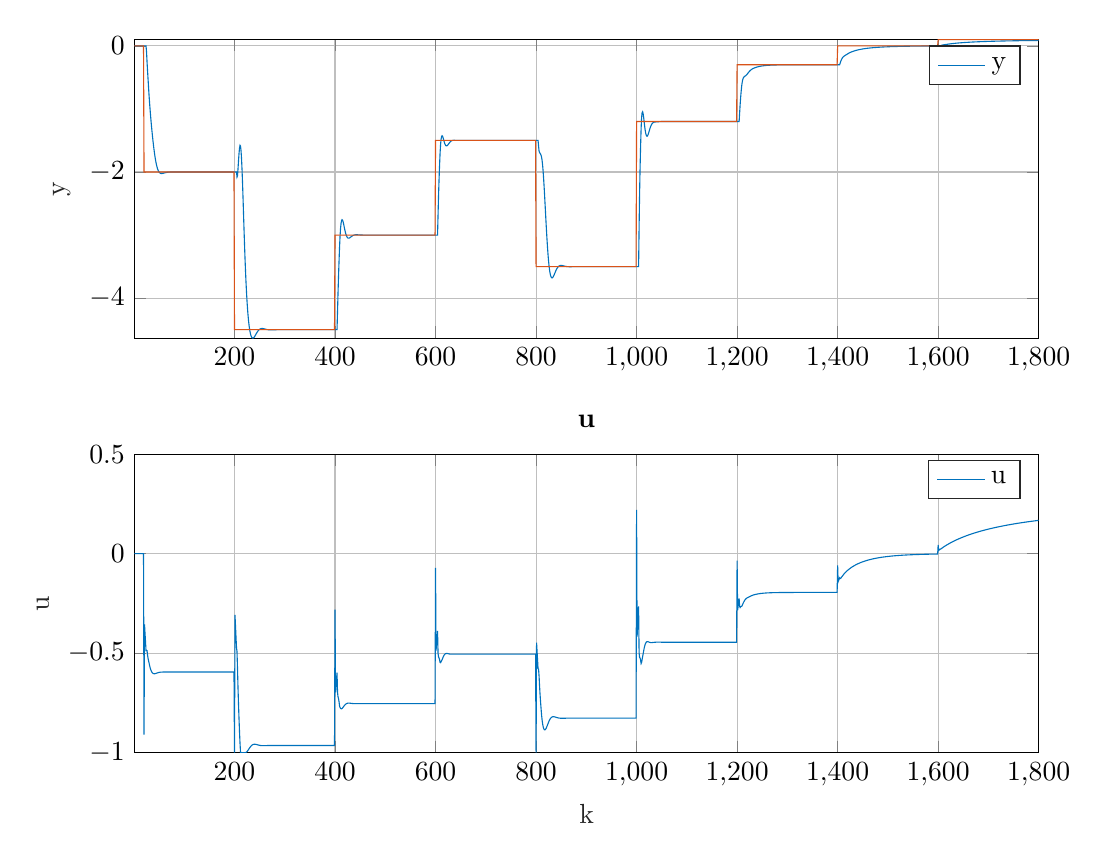
\begin{tikzpicture}

\begin{axis}[%
width=4.521in,
height=1.493in,
at={(0.758in,2.554in)},
scale only axis,
xmin=1,
xmax=1800,
ymin=-4.6335,
ymax=0.1,
ylabel style={font=\color{white!15!black}},
ylabel={y},
axis background/.style={fill=white},
xmajorgrids,
ymajorgrids,
legend style={legend cell align=left, align=left, draw=white!15!black}
]
\addplot [color=mycolor1]
  table[row sep=crcr]{%
1	0\\
2	0\\
3	0\\
4	0\\
5	0\\
6	0\\
7	0\\
8	0\\
9	0\\
10	0\\
11	0\\
12	0\\
13	0\\
14	0\\
15	0\\
16	0\\
17	0\\
18	0\\
19	0\\
20	0\\
21	0\\
22	0\\
23	0\\
24	0\\
25	-0.098378\\
26	-0.25368\\
27	-0.39312\\
28	-0.52557\\
29	-0.65731\\
30	-0.78382\\
31	-0.89914\\
32	-1.0051\\
33	-1.1044\\
34	-1.1976\\
35	-1.2852\\
36	-1.3679\\
37	-1.4461\\
38	-1.5199\\
39	-1.589\\
40	-1.6533\\
41	-1.7125\\
42	-1.7662\\
43	-1.8144\\
44	-1.8568\\
45	-1.8936\\
46	-1.9249\\
47	-1.951\\
48	-1.9721\\
49	-1.9889\\
50	-2.0016\\
51	-2.011\\
52	-2.0174\\
53	-2.0215\\
54	-2.0236\\
55	-2.0242\\
56	-2.0237\\
57	-2.0225\\
58	-2.0207\\
59	-2.0186\\
60	-2.0164\\
61	-2.0142\\
62	-2.0121\\
63	-2.0102\\
64	-2.0085\\
65	-2.0069\\
66	-2.0056\\
67	-2.0044\\
68	-2.0034\\
69	-2.0026\\
70	-2.002\\
71	-2.0014\\
72	-2.001\\
73	-2.0006\\
74	-2.0004\\
75	-2.0002\\
76	-2\\
77	-1.9999\\
78	-1.9998\\
79	-1.9998\\
80	-1.9997\\
81	-1.9997\\
82	-1.9997\\
83	-1.9997\\
84	-1.9997\\
85	-1.9997\\
86	-1.9998\\
87	-1.9998\\
88	-1.9998\\
89	-1.9998\\
90	-1.9999\\
91	-1.9999\\
92	-1.9999\\
93	-1.9999\\
94	-1.9999\\
95	-1.9999\\
96	-2\\
97	-2\\
98	-2\\
99	-2\\
100	-2\\
101	-2\\
102	-2\\
103	-2\\
104	-2\\
105	-2\\
106	-2\\
107	-2\\
108	-2\\
109	-2\\
110	-2\\
111	-2\\
112	-2\\
113	-2\\
114	-2\\
115	-2\\
116	-2\\
117	-2\\
118	-2\\
119	-2\\
120	-2\\
121	-2\\
122	-2\\
123	-2\\
124	-2\\
125	-2\\
126	-2\\
127	-2\\
128	-2\\
129	-2\\
130	-2\\
131	-2\\
132	-2\\
133	-2\\
134	-2\\
135	-2\\
136	-2\\
137	-2\\
138	-2\\
139	-2\\
140	-2\\
141	-2\\
142	-2\\
143	-2\\
144	-2\\
145	-2\\
146	-2\\
147	-2\\
148	-2\\
149	-2\\
150	-2\\
151	-2\\
152	-2\\
153	-2\\
154	-2\\
155	-2\\
156	-2\\
157	-2\\
158	-2\\
159	-2\\
160	-2\\
161	-2\\
162	-2\\
163	-2\\
164	-2\\
165	-2\\
166	-2\\
167	-2\\
168	-2\\
169	-2\\
170	-2\\
171	-2\\
172	-2\\
173	-2\\
174	-2\\
175	-2\\
176	-2\\
177	-2\\
178	-2\\
179	-2\\
180	-2\\
181	-2\\
182	-2\\
183	-2\\
184	-2\\
185	-2\\
186	-2\\
187	-2\\
188	-2\\
189	-2\\
190	-2\\
191	-2\\
192	-2\\
193	-2\\
194	-2\\
195	-2\\
196	-2\\
197	-2\\
198	-2\\
199	-2\\
200	-2\\
201	-2\\
202	-2\\
203	-2\\
204	-2\\
205	-2.0801\\
206	-2.0594\\
207	-1.9505\\
208	-1.8212\\
209	-1.7083\\
210	-1.6218\\
211	-1.578\\
212	-1.5904\\
213	-1.6617\\
214	-1.7873\\
215	-1.9604\\
216	-2.1727\\
217	-2.4144\\
218	-2.6692\\
219	-2.9216\\
220	-3.1617\\
221	-3.3836\\
222	-3.5845\\
223	-3.7634\\
224	-3.9207\\
225	-4.0574\\
226	-4.1752\\
227	-4.2758\\
228	-4.3608\\
229	-4.4317\\
230	-4.4898\\
231	-4.5363\\
232	-4.5724\\
233	-4.5992\\
234	-4.6177\\
235	-4.6288\\
236	-4.6335\\
237	-4.6329\\
238	-4.6279\\
239	-4.6195\\
240	-4.6084\\
241	-4.5957\\
242	-4.5819\\
243	-4.5677\\
244	-4.5538\\
245	-4.5405\\
246	-4.5283\\
247	-4.5174\\
248	-4.5078\\
249	-4.4999\\
250	-4.4934\\
251	-4.4884\\
252	-4.4849\\
253	-4.4826\\
254	-4.4814\\
255	-4.4811\\
256	-4.4817\\
257	-4.4828\\
258	-4.4844\\
259	-4.4863\\
260	-4.4883\\
261	-4.4904\\
262	-4.4925\\
263	-4.4944\\
264	-4.4962\\
265	-4.4978\\
266	-4.4992\\
267	-4.5003\\
268	-4.5012\\
269	-4.5019\\
270	-4.5024\\
271	-4.5027\\
272	-4.5028\\
273	-4.5028\\
274	-4.5027\\
275	-4.5025\\
276	-4.5022\\
277	-4.5019\\
278	-4.5016\\
279	-4.5013\\
280	-4.501\\
281	-4.5007\\
282	-4.5005\\
283	-4.5002\\
284	-4.5\\
285	-4.4999\\
286	-4.4998\\
287	-4.4997\\
288	-4.4996\\
289	-4.4996\\
290	-4.4996\\
291	-4.4996\\
292	-4.4996\\
293	-4.4996\\
294	-4.4997\\
295	-4.4997\\
296	-4.4998\\
297	-4.4998\\
298	-4.4999\\
299	-4.4999\\
300	-4.4999\\
301	-4.5\\
302	-4.5\\
303	-4.5\\
304	-4.5\\
305	-4.5001\\
306	-4.5001\\
307	-4.5001\\
308	-4.5001\\
309	-4.5001\\
310	-4.5001\\
311	-4.5001\\
312	-4.5\\
313	-4.5\\
314	-4.5\\
315	-4.5\\
316	-4.5\\
317	-4.5\\
318	-4.5\\
319	-4.5\\
320	-4.5\\
321	-4.5\\
322	-4.5\\
323	-4.5\\
324	-4.5\\
325	-4.5\\
326	-4.5\\
327	-4.5\\
328	-4.5\\
329	-4.5\\
330	-4.5\\
331	-4.5\\
332	-4.5\\
333	-4.5\\
334	-4.5\\
335	-4.5\\
336	-4.5\\
337	-4.5\\
338	-4.5\\
339	-4.5\\
340	-4.5\\
341	-4.5\\
342	-4.5\\
343	-4.5\\
344	-4.5\\
345	-4.5\\
346	-4.5\\
347	-4.5\\
348	-4.5\\
349	-4.5\\
350	-4.5\\
351	-4.5\\
352	-4.5\\
353	-4.5\\
354	-4.5\\
355	-4.5\\
356	-4.5\\
357	-4.5\\
358	-4.5\\
359	-4.5\\
360	-4.5\\
361	-4.5\\
362	-4.5\\
363	-4.5\\
364	-4.5\\
365	-4.5\\
366	-4.5\\
367	-4.5\\
368	-4.5\\
369	-4.5\\
370	-4.5\\
371	-4.5\\
372	-4.5\\
373	-4.5\\
374	-4.5\\
375	-4.5\\
376	-4.5\\
377	-4.5\\
378	-4.5\\
379	-4.5\\
380	-4.5\\
381	-4.5\\
382	-4.5\\
383	-4.5\\
384	-4.5\\
385	-4.5\\
386	-4.5\\
387	-4.5\\
388	-4.5\\
389	-4.5\\
390	-4.5\\
391	-4.5\\
392	-4.5\\
393	-4.5\\
394	-4.5\\
395	-4.5\\
396	-4.5\\
397	-4.5\\
398	-4.5\\
399	-4.5\\
400	-4.5\\
401	-4.5\\
402	-4.5\\
403	-4.5\\
404	-4.5\\
405	-4.2111\\
406	-3.9122\\
407	-3.6513\\
408	-3.4154\\
409	-3.1953\\
410	-3.0205\\
411	-2.8973\\
412	-2.8167\\
413	-2.7711\\
414	-2.7555\\
415	-2.7635\\
416	-2.7875\\
417	-2.8211\\
418	-2.8594\\
419	-2.8985\\
420	-2.9354\\
421	-2.968\\
422	-2.9952\\
423	-3.0166\\
424	-3.0322\\
425	-3.0424\\
426	-3.0479\\
427	-3.0495\\
428	-3.0481\\
429	-3.0444\\
430	-3.0392\\
431	-3.0333\\
432	-3.0271\\
433	-3.021\\
434	-3.0153\\
435	-3.0103\\
436	-3.006\\
437	-3.0025\\
438	-2.9998\\
439	-2.9977\\
440	-2.9964\\
441	-2.9955\\
442	-2.9951\\
443	-2.9951\\
444	-2.9953\\
445	-2.9957\\
446	-2.9962\\
447	-2.9967\\
448	-2.9973\\
449	-2.9978\\
450	-2.9983\\
451	-2.9988\\
452	-2.9992\\
453	-2.9995\\
454	-2.9997\\
455	-2.9999\\
456	-3.0001\\
457	-3.0002\\
458	-3.0003\\
459	-3.0003\\
460	-3.0003\\
461	-3.0003\\
462	-3.0003\\
463	-3.0003\\
464	-3.0002\\
465	-3.0002\\
466	-3.0002\\
467	-3.0001\\
468	-3.0001\\
469	-3.0001\\
470	-3.0001\\
471	-3\\
472	-3\\
473	-3\\
474	-3\\
475	-3\\
476	-3\\
477	-3\\
478	-3\\
479	-3\\
480	-3\\
481	-3\\
482	-3\\
483	-3\\
484	-3\\
485	-3\\
486	-3\\
487	-3\\
488	-3\\
489	-3\\
490	-3\\
491	-3\\
492	-3\\
493	-3\\
494	-3\\
495	-3\\
496	-3\\
497	-3\\
498	-3\\
499	-3\\
500	-3\\
501	-3\\
502	-3\\
503	-3\\
504	-3\\
505	-3\\
506	-3\\
507	-3\\
508	-3\\
509	-3\\
510	-3\\
511	-3\\
512	-3\\
513	-3\\
514	-3\\
515	-3\\
516	-3\\
517	-3\\
518	-3\\
519	-3\\
520	-3\\
521	-3\\
522	-3\\
523	-3\\
524	-3\\
525	-3\\
526	-3\\
527	-3\\
528	-3\\
529	-3\\
530	-3\\
531	-3\\
532	-3\\
533	-3\\
534	-3\\
535	-3\\
536	-3\\
537	-3\\
538	-3\\
539	-3\\
540	-3\\
541	-3\\
542	-3\\
543	-3\\
544	-3\\
545	-3\\
546	-3\\
547	-3\\
548	-3\\
549	-3\\
550	-3\\
551	-3\\
552	-3\\
553	-3\\
554	-3\\
555	-3\\
556	-3\\
557	-3\\
558	-3\\
559	-3\\
560	-3\\
561	-3\\
562	-3\\
563	-3\\
564	-3\\
565	-3\\
566	-3\\
567	-3\\
568	-3\\
569	-3\\
570	-3\\
571	-3\\
572	-3\\
573	-3\\
574	-3\\
575	-3\\
576	-3\\
577	-3\\
578	-3\\
579	-3\\
580	-3\\
581	-3\\
582	-3\\
583	-3\\
584	-3\\
585	-3\\
586	-3\\
587	-3\\
588	-3\\
589	-3\\
590	-3\\
591	-3\\
592	-3\\
593	-3\\
594	-3\\
595	-3\\
596	-3\\
597	-3\\
598	-3\\
599	-3\\
600	-3\\
601	-3\\
602	-3\\
603	-3\\
604	-3\\
605	-2.6784\\
606	-2.37\\
607	-2.1158\\
608	-1.8985\\
609	-1.706\\
610	-1.5671\\
611	-1.4829\\
612	-1.4393\\
613	-1.4251\\
614	-1.4334\\
615	-1.4562\\
616	-1.4855\\
617	-1.5153\\
618	-1.542\\
619	-1.5631\\
620	-1.5775\\
621	-1.5851\\
622	-1.5865\\
623	-1.5829\\
624	-1.5755\\
625	-1.5658\\
626	-1.5549\\
627	-1.5439\\
628	-1.5334\\
629	-1.5242\\
630	-1.5164\\
631	-1.5101\\
632	-1.5054\\
633	-1.502\\
634	-1.4998\\
635	-1.4985\\
636	-1.4979\\
637	-1.4977\\
638	-1.4979\\
639	-1.4982\\
640	-1.4986\\
641	-1.499\\
642	-1.4993\\
643	-1.4995\\
644	-1.4997\\
645	-1.4997\\
646	-1.4998\\
647	-1.4998\\
648	-1.4997\\
649	-1.4997\\
650	-1.4996\\
651	-1.4996\\
652	-1.4996\\
653	-1.4996\\
654	-1.4996\\
655	-1.4996\\
656	-1.4997\\
657	-1.4997\\
658	-1.4997\\
659	-1.4998\\
660	-1.4998\\
661	-1.4999\\
662	-1.4999\\
663	-1.4999\\
664	-1.4999\\
665	-1.5\\
666	-1.5\\
667	-1.5\\
668	-1.5\\
669	-1.5\\
670	-1.5\\
671	-1.5\\
672	-1.5\\
673	-1.5\\
674	-1.5\\
675	-1.5\\
676	-1.5\\
677	-1.5\\
678	-1.5\\
679	-1.5\\
680	-1.5\\
681	-1.5\\
682	-1.5\\
683	-1.5\\
684	-1.5\\
685	-1.5\\
686	-1.5\\
687	-1.5\\
688	-1.5\\
689	-1.5\\
690	-1.5\\
691	-1.5\\
692	-1.5\\
693	-1.5\\
694	-1.5\\
695	-1.5\\
696	-1.5\\
697	-1.5\\
698	-1.5\\
699	-1.5\\
700	-1.5\\
701	-1.5\\
702	-1.5\\
703	-1.5\\
704	-1.5\\
705	-1.5\\
706	-1.5\\
707	-1.5\\
708	-1.5\\
709	-1.5\\
710	-1.5\\
711	-1.5\\
712	-1.5\\
713	-1.5\\
714	-1.5\\
715	-1.5\\
716	-1.5\\
717	-1.5\\
718	-1.5\\
719	-1.5\\
720	-1.5\\
721	-1.5\\
722	-1.5\\
723	-1.5\\
724	-1.5\\
725	-1.5\\
726	-1.5\\
727	-1.5\\
728	-1.5\\
729	-1.5\\
730	-1.5\\
731	-1.5\\
732	-1.5\\
733	-1.5\\
734	-1.5\\
735	-1.5\\
736	-1.5\\
737	-1.5\\
738	-1.5\\
739	-1.5\\
740	-1.5\\
741	-1.5\\
742	-1.5\\
743	-1.5\\
744	-1.5\\
745	-1.5\\
746	-1.5\\
747	-1.5\\
748	-1.5\\
749	-1.5\\
750	-1.5\\
751	-1.5\\
752	-1.5\\
753	-1.5\\
754	-1.5\\
755	-1.5\\
756	-1.5\\
757	-1.5\\
758	-1.5\\
759	-1.5\\
760	-1.5\\
761	-1.5\\
762	-1.5\\
763	-1.5\\
764	-1.5\\
765	-1.5\\
766	-1.5\\
767	-1.5\\
768	-1.5\\
769	-1.5\\
770	-1.5\\
771	-1.5\\
772	-1.5\\
773	-1.5\\
774	-1.5\\
775	-1.5\\
776	-1.5\\
777	-1.5\\
778	-1.5\\
779	-1.5\\
780	-1.5\\
781	-1.5\\
782	-1.5\\
783	-1.5\\
784	-1.5\\
785	-1.5\\
786	-1.5\\
787	-1.5\\
788	-1.5\\
789	-1.5\\
790	-1.5\\
791	-1.5\\
792	-1.5\\
793	-1.5\\
794	-1.5\\
795	-1.5\\
796	-1.5\\
797	-1.5\\
798	-1.5\\
799	-1.5\\
800	-1.5\\
801	-1.5\\
802	-1.5\\
803	-1.5\\
804	-1.5\\
805	-1.593\\
806	-1.6684\\
807	-1.6941\\
808	-1.7035\\
809	-1.717\\
810	-1.7365\\
811	-1.7668\\
812	-1.8165\\
813	-1.8893\\
814	-1.9843\\
815	-2.0988\\
816	-2.2295\\
817	-2.3721\\
818	-2.5216\\
819	-2.6732\\
820	-2.8226\\
821	-2.9658\\
822	-3.0995\\
823	-3.2213\\
824	-3.3292\\
825	-3.4223\\
826	-3.4999\\
827	-3.5623\\
828	-3.6101\\
829	-3.6442\\
830	-3.666\\
831	-3.6771\\
832	-3.6791\\
833	-3.6737\\
834	-3.6627\\
835	-3.6476\\
836	-3.6298\\
837	-3.6107\\
838	-3.5912\\
839	-3.5723\\
840	-3.5545\\
841	-3.5385\\
842	-3.5244\\
843	-3.5124\\
844	-3.5026\\
845	-3.4949\\
846	-3.4892\\
847	-3.4852\\
848	-3.4827\\
849	-3.4815\\
850	-3.4813\\
851	-3.482\\
852	-3.4833\\
853	-3.4849\\
854	-3.4869\\
855	-3.4889\\
856	-3.4909\\
857	-3.4929\\
858	-3.4947\\
859	-3.4963\\
860	-3.4977\\
861	-3.4988\\
862	-3.4998\\
863	-3.5005\\
864	-3.5011\\
865	-3.5014\\
866	-3.5017\\
867	-3.5018\\
868	-3.5018\\
869	-3.5017\\
870	-3.5016\\
871	-3.5014\\
872	-3.5012\\
873	-3.5011\\
874	-3.5009\\
875	-3.5007\\
876	-3.5005\\
877	-3.5004\\
878	-3.5002\\
879	-3.5001\\
880	-3.5\\
881	-3.5\\
882	-3.4999\\
883	-3.4999\\
884	-3.4998\\
885	-3.4998\\
886	-3.4998\\
887	-3.4998\\
888	-3.4999\\
889	-3.4999\\
890	-3.4999\\
891	-3.4999\\
892	-3.4999\\
893	-3.4999\\
894	-3.5\\
895	-3.5\\
896	-3.5\\
897	-3.5\\
898	-3.5\\
899	-3.5\\
900	-3.5\\
901	-3.5\\
902	-3.5\\
903	-3.5\\
904	-3.5\\
905	-3.5\\
906	-3.5\\
907	-3.5\\
908	-3.5\\
909	-3.5\\
910	-3.5\\
911	-3.5\\
912	-3.5\\
913	-3.5\\
914	-3.5\\
915	-3.5\\
916	-3.5\\
917	-3.5\\
918	-3.5\\
919	-3.5\\
920	-3.5\\
921	-3.5\\
922	-3.5\\
923	-3.5\\
924	-3.5\\
925	-3.5\\
926	-3.5\\
927	-3.5\\
928	-3.5\\
929	-3.5\\
930	-3.5\\
931	-3.5\\
932	-3.5\\
933	-3.5\\
934	-3.5\\
935	-3.5\\
936	-3.5\\
937	-3.5\\
938	-3.5\\
939	-3.5\\
940	-3.5\\
941	-3.5\\
942	-3.5\\
943	-3.5\\
944	-3.5\\
945	-3.5\\
946	-3.5\\
947	-3.5\\
948	-3.5\\
949	-3.5\\
950	-3.5\\
951	-3.5\\
952	-3.5\\
953	-3.5\\
954	-3.5\\
955	-3.5\\
956	-3.5\\
957	-3.5\\
958	-3.5\\
959	-3.5\\
960	-3.5\\
961	-3.5\\
962	-3.5\\
963	-3.5\\
964	-3.5\\
965	-3.5\\
966	-3.5\\
967	-3.5\\
968	-3.5\\
969	-3.5\\
970	-3.5\\
971	-3.5\\
972	-3.5\\
973	-3.5\\
974	-3.5\\
975	-3.5\\
976	-3.5\\
977	-3.5\\
978	-3.5\\
979	-3.5\\
980	-3.5\\
981	-3.5\\
982	-3.5\\
983	-3.5\\
984	-3.5\\
985	-3.5\\
986	-3.5\\
987	-3.5\\
988	-3.5\\
989	-3.5\\
990	-3.5\\
991	-3.5\\
992	-3.5\\
993	-3.5\\
994	-3.5\\
995	-3.5\\
996	-3.5\\
997	-3.5\\
998	-3.5\\
999	-3.5\\
1000	-3.5\\
1001	-3.5\\
1002	-3.5\\
1003	-3.5\\
1004	-3.5\\
1005	-2.8781\\
1006	-2.3361\\
1007	-1.9185\\
1008	-1.5862\\
1009	-1.312\\
1010	-1.138\\
1011	-1.0595\\
1012	-1.0456\\
1013	-1.0737\\
1014	-1.1298\\
1015	-1.1999\\
1016	-1.2704\\
1017	-1.3323\\
1018	-1.3808\\
1019	-1.4136\\
1020	-1.4304\\
1021	-1.4326\\
1022	-1.4228\\
1023	-1.4044\\
1024	-1.3804\\
1025	-1.3538\\
1026	-1.3269\\
1027	-1.3017\\
1028	-1.2792\\
1029	-1.2602\\
1030	-1.2448\\
1031	-1.2328\\
1032	-1.2239\\
1033	-1.2176\\
1034	-1.2133\\
1035	-1.2105\\
1036	-1.2087\\
1037	-1.2076\\
1038	-1.2069\\
1039	-1.2063\\
1040	-1.2057\\
1041	-1.2051\\
1042	-1.2045\\
1043	-1.2038\\
1044	-1.2031\\
1045	-1.2024\\
1046	-1.2018\\
1047	-1.2012\\
1048	-1.2007\\
1049	-1.2003\\
1050	-1.2\\
1051	-1.1998\\
1052	-1.1997\\
1053	-1.1996\\
1054	-1.1995\\
1055	-1.1995\\
1056	-1.1995\\
1057	-1.1996\\
1058	-1.1996\\
1059	-1.1997\\
1060	-1.1997\\
1061	-1.1998\\
1062	-1.1998\\
1063	-1.1998\\
1064	-1.1999\\
1065	-1.1999\\
1066	-1.1999\\
1067	-1.1999\\
1068	-1.1999\\
1069	-1.1999\\
1070	-1.1999\\
1071	-1.1999\\
1072	-1.1999\\
1073	-1.2\\
1074	-1.2\\
1075	-1.2\\
1076	-1.2\\
1077	-1.2\\
1078	-1.2\\
1079	-1.2\\
1080	-1.2\\
1081	-1.2\\
1082	-1.2\\
1083	-1.2\\
1084	-1.2\\
1085	-1.2\\
1086	-1.2\\
1087	-1.2\\
1088	-1.2\\
1089	-1.2\\
1090	-1.2\\
1091	-1.2\\
1092	-1.2\\
1093	-1.2\\
1094	-1.2\\
1095	-1.2\\
1096	-1.2\\
1097	-1.2\\
1098	-1.2\\
1099	-1.2\\
1100	-1.2\\
1101	-1.2\\
1102	-1.2\\
1103	-1.2\\
1104	-1.2\\
1105	-1.2\\
1106	-1.2\\
1107	-1.2\\
1108	-1.2\\
1109	-1.2\\
1110	-1.2\\
1111	-1.2\\
1112	-1.2\\
1113	-1.2\\
1114	-1.2\\
1115	-1.2\\
1116	-1.2\\
1117	-1.2\\
1118	-1.2\\
1119	-1.2\\
1120	-1.2\\
1121	-1.2\\
1122	-1.2\\
1123	-1.2\\
1124	-1.2\\
1125	-1.2\\
1126	-1.2\\
1127	-1.2\\
1128	-1.2\\
1129	-1.2\\
1130	-1.2\\
1131	-1.2\\
1132	-1.2\\
1133	-1.2\\
1134	-1.2\\
1135	-1.2\\
1136	-1.2\\
1137	-1.2\\
1138	-1.2\\
1139	-1.2\\
1140	-1.2\\
1141	-1.2\\
1142	-1.2\\
1143	-1.2\\
1144	-1.2\\
1145	-1.2\\
1146	-1.2\\
1147	-1.2\\
1148	-1.2\\
1149	-1.2\\
1150	-1.2\\
1151	-1.2\\
1152	-1.2\\
1153	-1.2\\
1154	-1.2\\
1155	-1.2\\
1156	-1.2\\
1157	-1.2\\
1158	-1.2\\
1159	-1.2\\
1160	-1.2\\
1161	-1.2\\
1162	-1.2\\
1163	-1.2\\
1164	-1.2\\
1165	-1.2\\
1166	-1.2\\
1167	-1.2\\
1168	-1.2\\
1169	-1.2\\
1170	-1.2\\
1171	-1.2\\
1172	-1.2\\
1173	-1.2\\
1174	-1.2\\
1175	-1.2\\
1176	-1.2\\
1177	-1.2\\
1178	-1.2\\
1179	-1.2\\
1180	-1.2\\
1181	-1.2\\
1182	-1.2\\
1183	-1.2\\
1184	-1.2\\
1185	-1.2\\
1186	-1.2\\
1187	-1.2\\
1188	-1.2\\
1189	-1.2\\
1190	-1.2\\
1191	-1.2\\
1192	-1.2\\
1193	-1.2\\
1194	-1.2\\
1195	-1.2\\
1196	-1.2\\
1197	-1.2\\
1198	-1.2\\
1199	-1.2\\
1200	-1.2\\
1201	-1.2\\
1202	-1.2\\
1203	-1.2\\
1204	-1.2\\
1205	-1.0699\\
1206	-0.9347\\
1207	-0.82309\\
1208	-0.72852\\
1209	-0.64625\\
1210	-0.58455\\
1211	-0.5436\\
1212	-0.51734\\
1213	-0.5008\\
1214	-0.49082\\
1215	-0.4845\\
1216	-0.47924\\
1217	-0.47348\\
1218	-0.46657\\
1219	-0.45837\\
1220	-0.44907\\
1221	-0.43906\\
1222	-0.4288\\
1223	-0.41874\\
1224	-0.40918\\
1225	-0.40036\\
1226	-0.39236\\
1227	-0.38522\\
1228	-0.37887\\
1229	-0.37324\\
1230	-0.36821\\
1231	-0.36369\\
1232	-0.35958\\
1233	-0.3558\\
1234	-0.3523\\
1235	-0.34904\\
1236	-0.34597\\
1237	-0.3431\\
1238	-0.3404\\
1239	-0.33786\\
1240	-0.33549\\
1241	-0.33326\\
1242	-0.33118\\
1243	-0.32924\\
1244	-0.32743\\
1245	-0.32574\\
1246	-0.32417\\
1247	-0.3227\\
1248	-0.32132\\
1249	-0.32003\\
1250	-0.31883\\
1251	-0.3177\\
1252	-0.31664\\
1253	-0.31564\\
1254	-0.31471\\
1255	-0.31383\\
1256	-0.31301\\
1257	-0.31224\\
1258	-0.31151\\
1259	-0.31083\\
1260	-0.31019\\
1261	-0.30959\\
1262	-0.30903\\
1263	-0.30849\\
1264	-0.308\\
1265	-0.30753\\
1266	-0.30709\\
1267	-0.30667\\
1268	-0.30628\\
1269	-0.30591\\
1270	-0.30557\\
1271	-0.30524\\
1272	-0.30494\\
1273	-0.30465\\
1274	-0.30438\\
1275	-0.30412\\
1276	-0.30388\\
1277	-0.30366\\
1278	-0.30344\\
1279	-0.30324\\
1280	-0.30306\\
1281	-0.30288\\
1282	-0.30271\\
1283	-0.30255\\
1284	-0.30241\\
1285	-0.30227\\
1286	-0.30214\\
1287	-0.30201\\
1288	-0.30189\\
1289	-0.30179\\
1290	-0.30168\\
1291	-0.30158\\
1292	-0.30149\\
1293	-0.30141\\
1294	-0.30132\\
1295	-0.30125\\
1296	-0.30118\\
1297	-0.30111\\
1298	-0.30104\\
1299	-0.30098\\
1300	-0.30093\\
1301	-0.30087\\
1302	-0.30082\\
1303	-0.30078\\
1304	-0.30073\\
1305	-0.30069\\
1306	-0.30065\\
1307	-0.30061\\
1308	-0.30058\\
1309	-0.30054\\
1310	-0.30051\\
1311	-0.30048\\
1312	-0.30045\\
1313	-0.30043\\
1314	-0.3004\\
1315	-0.30038\\
1316	-0.30036\\
1317	-0.30034\\
1318	-0.30032\\
1319	-0.3003\\
1320	-0.30028\\
1321	-0.30027\\
1322	-0.30025\\
1323	-0.30024\\
1324	-0.30022\\
1325	-0.30021\\
1326	-0.3002\\
1327	-0.30019\\
1328	-0.30018\\
1329	-0.30017\\
1330	-0.30016\\
1331	-0.30015\\
1332	-0.30014\\
1333	-0.30013\\
1334	-0.30012\\
1335	-0.30012\\
1336	-0.30011\\
1337	-0.3001\\
1338	-0.3001\\
1339	-0.30009\\
1340	-0.30009\\
1341	-0.30008\\
1342	-0.30008\\
1343	-0.30007\\
1344	-0.30007\\
1345	-0.30006\\
1346	-0.30006\\
1347	-0.30006\\
1348	-0.30005\\
1349	-0.30005\\
1350	-0.30005\\
1351	-0.30004\\
1352	-0.30004\\
1353	-0.30004\\
1354	-0.30004\\
1355	-0.30004\\
1356	-0.30003\\
1357	-0.30003\\
1358	-0.30003\\
1359	-0.30003\\
1360	-0.30003\\
1361	-0.30002\\
1362	-0.30002\\
1363	-0.30002\\
1364	-0.30002\\
1365	-0.30002\\
1366	-0.30002\\
1367	-0.30002\\
1368	-0.30002\\
1369	-0.30002\\
1370	-0.30001\\
1371	-0.30001\\
1372	-0.30001\\
1373	-0.30001\\
1374	-0.30001\\
1375	-0.30001\\
1376	-0.30001\\
1377	-0.30001\\
1378	-0.30001\\
1379	-0.30001\\
1380	-0.30001\\
1381	-0.30001\\
1382	-0.30001\\
1383	-0.30001\\
1384	-0.30001\\
1385	-0.30001\\
1386	-0.30001\\
1387	-0.30001\\
1388	-0.3\\
1389	-0.3\\
1390	-0.3\\
1391	-0.3\\
1392	-0.3\\
1393	-0.3\\
1394	-0.3\\
1395	-0.3\\
1396	-0.3\\
1397	-0.3\\
1398	-0.3\\
1399	-0.3\\
1400	-0.3\\
1401	-0.3\\
1402	-0.3\\
1403	-0.3\\
1404	-0.3\\
1405	-0.2777\\
1406	-0.25099\\
1407	-0.22962\\
1408	-0.21197\\
1409	-0.19682\\
1410	-0.18468\\
1411	-0.17556\\
1412	-0.16843\\
1413	-0.16241\\
1414	-0.15703\\
1415	-0.15197\\
1416	-0.14699\\
1417	-0.14201\\
1418	-0.13702\\
1419	-0.13207\\
1420	-0.12722\\
1421	-0.12252\\
1422	-0.11802\\
1423	-0.11374\\
1424	-0.10968\\
1425	-0.10584\\
1426	-0.10221\\
1427	-0.098772\\
1428	-0.095507\\
1429	-0.092401\\
1430	-0.089439\\
1431	-0.086609\\
1432	-0.0839\\
1433	-0.081305\\
1434	-0.078818\\
1435	-0.076431\\
1436	-0.07414\\
1437	-0.07194\\
1438	-0.069826\\
1439	-0.067794\\
1440	-0.06584\\
1441	-0.063961\\
1442	-0.062151\\
1443	-0.060408\\
1444	-0.058729\\
1445	-0.05711\\
1446	-0.055548\\
1447	-0.054041\\
1448	-0.052586\\
1449	-0.051181\\
1450	-0.049823\\
1451	-0.04851\\
1452	-0.047241\\
1453	-0.046014\\
1454	-0.044826\\
1455	-0.043676\\
1456	-0.042563\\
1457	-0.041484\\
1458	-0.040439\\
1459	-0.039427\\
1460	-0.038445\\
1461	-0.037493\\
1462	-0.03657\\
1463	-0.035674\\
1464	-0.034804\\
1465	-0.03396\\
1466	-0.03314\\
1467	-0.032344\\
1468	-0.031571\\
1469	-0.030819\\
1470	-0.030089\\
1471	-0.029379\\
1472	-0.028689\\
1473	-0.028018\\
1474	-0.027365\\
1475	-0.02673\\
1476	-0.026112\\
1477	-0.02551\\
1478	-0.024925\\
1479	-0.024355\\
1480	-0.0238\\
1481	-0.02326\\
1482	-0.022733\\
1483	-0.02222\\
1484	-0.021721\\
1485	-0.021234\\
1486	-0.02076\\
1487	-0.020297\\
1488	-0.019846\\
1489	-0.019407\\
1490	-0.018978\\
1491	-0.01856\\
1492	-0.018153\\
1493	-0.017755\\
1494	-0.017367\\
1495	-0.016988\\
1496	-0.016619\\
1497	-0.016259\\
1498	-0.015907\\
1499	-0.015564\\
1500	-0.015228\\
1501	-0.014901\\
1502	-0.014582\\
1503	-0.01427\\
1504	-0.013965\\
1505	-0.013667\\
1506	-0.013377\\
1507	-0.013093\\
1508	-0.012815\\
1509	-0.012544\\
1510	-0.01228\\
1511	-0.012021\\
1512	-0.011768\\
1513	-0.011521\\
1514	-0.01128\\
1515	-0.011044\\
1516	-0.010813\\
1517	-0.010587\\
1518	-0.010367\\
1519	-0.010151\\
1520	-0.0099404\\
1521	-0.0097343\\
1522	-0.0095328\\
1523	-0.0093357\\
1524	-0.009143\\
1525	-0.0089545\\
1526	-0.0087701\\
1527	-0.0085897\\
1528	-0.0084133\\
1529	-0.0082407\\
1530	-0.0080719\\
1531	-0.0079067\\
1532	-0.0077451\\
1533	-0.0075869\\
1534	-0.0074322\\
1535	-0.0072808\\
1536	-0.0071326\\
1537	-0.0069876\\
1538	-0.0068457\\
1539	-0.0067068\\
1540	-0.0065709\\
1541	-0.0064378\\
1542	-0.0063076\\
1543	-0.0061801\\
1544	-0.0060553\\
1545	-0.0059332\\
1546	-0.0058136\\
1547	-0.0056965\\
1548	-0.0055819\\
1549	-0.0054696\\
1550	-0.0053597\\
1551	-0.0052521\\
1552	-0.0051468\\
1553	-0.0050436\\
1554	-0.0049426\\
1555	-0.0048437\\
1556	-0.0047468\\
1557	-0.004652\\
1558	-0.0045591\\
1559	-0.0044681\\
1560	-0.0043789\\
1561	-0.0042917\\
1562	-0.0042062\\
1563	-0.0041224\\
1564	-0.0040404\\
1565	-0.0039601\\
1566	-0.0038814\\
1567	-0.0038043\\
1568	-0.0037288\\
1569	-0.0036548\\
1570	-0.0035823\\
1571	-0.0035114\\
1572	-0.0034418\\
1573	-0.0033737\\
1574	-0.0033069\\
1575	-0.0032415\\
1576	-0.0031774\\
1577	-0.0031146\\
1578	-0.0030531\\
1579	-0.0029929\\
1580	-0.0029338\\
1581	-0.0028759\\
1582	-0.0028192\\
1583	-0.0027637\\
1584	-0.0027092\\
1585	-0.0026559\\
1586	-0.0026036\\
1587	-0.0025524\\
1588	-0.0025022\\
1589	-0.002453\\
1590	-0.0024048\\
1591	-0.0023575\\
1592	-0.0023112\\
1593	-0.0022659\\
1594	-0.0022214\\
1595	-0.0021778\\
1596	-0.0021351\\
1597	-0.0020932\\
1598	-0.0020522\\
1599	-0.002012\\
1600	-0.0019726\\
1601	-0.0019339\\
1602	-0.0018961\\
1603	-0.001859\\
1604	-0.0018226\\
1605	0.0010104\\
1606	0.0054261\\
1607	0.0085557\\
1608	0.010921\\
1609	0.012857\\
1610	0.014497\\
1611	0.015877\\
1612	0.017104\\
1613	0.018289\\
1614	0.019473\\
1615	0.020666\\
1616	0.021868\\
1617	0.02307\\
1618	0.024265\\
1619	0.025443\\
1620	0.026598\\
1621	0.027724\\
1622	0.028822\\
1623	0.02989\\
1624	0.03093\\
1625	0.031942\\
1626	0.032928\\
1627	0.033889\\
1628	0.034826\\
1629	0.035741\\
1630	0.036634\\
1631	0.037506\\
1632	0.038358\\
1633	0.03919\\
1634	0.040004\\
1635	0.040799\\
1636	0.041576\\
1637	0.042336\\
1638	0.043079\\
1639	0.043806\\
1640	0.044518\\
1641	0.045214\\
1642	0.045896\\
1643	0.046563\\
1644	0.047217\\
1645	0.047858\\
1646	0.048485\\
1647	0.0491\\
1648	0.049703\\
1649	0.050293\\
1650	0.050873\\
1651	0.051441\\
1652	0.051998\\
1653	0.052544\\
1654	0.05308\\
1655	0.053607\\
1656	0.054123\\
1657	0.05463\\
1658	0.055128\\
1659	0.055617\\
1660	0.056097\\
1661	0.056569\\
1662	0.057032\\
1663	0.057487\\
1664	0.057934\\
1665	0.058374\\
1666	0.058806\\
1667	0.059231\\
1668	0.059649\\
1669	0.060059\\
1670	0.060463\\
1671	0.060861\\
1672	0.061251\\
1673	0.061636\\
1674	0.062014\\
1675	0.062387\\
1676	0.062753\\
1677	0.063114\\
1678	0.063469\\
1679	0.063819\\
1680	0.064163\\
1681	0.064502\\
1682	0.064836\\
1683	0.065165\\
1684	0.065489\\
1685	0.065808\\
1686	0.066122\\
1687	0.066432\\
1688	0.066738\\
1689	0.067039\\
1690	0.067335\\
1691	0.067628\\
1692	0.067916\\
1693	0.0682\\
1694	0.068481\\
1695	0.068757\\
1696	0.069029\\
1697	0.069298\\
1698	0.069563\\
1699	0.069825\\
1700	0.070083\\
1701	0.070338\\
1702	0.070589\\
1703	0.070837\\
1704	0.071082\\
1705	0.071323\\
1706	0.071561\\
1707	0.071797\\
1708	0.072029\\
1709	0.072258\\
1710	0.072484\\
1711	0.072708\\
1712	0.072929\\
1713	0.073147\\
1714	0.073362\\
1715	0.073575\\
1716	0.073785\\
1717	0.073992\\
1718	0.074197\\
1719	0.074399\\
1720	0.074599\\
1721	0.074797\\
1722	0.074992\\
1723	0.075185\\
1724	0.075376\\
1725	0.075565\\
1726	0.075751\\
1727	0.075935\\
1728	0.076117\\
1729	0.076297\\
1730	0.076475\\
1731	0.076651\\
1732	0.076825\\
1733	0.076997\\
1734	0.077167\\
1735	0.077335\\
1736	0.077501\\
1737	0.077666\\
1738	0.077828\\
1739	0.077989\\
1740	0.078149\\
1741	0.078306\\
1742	0.078462\\
1743	0.078616\\
1744	0.078768\\
1745	0.078919\\
1746	0.079068\\
1747	0.079216\\
1748	0.079362\\
1749	0.079507\\
1750	0.07965\\
1751	0.079792\\
1752	0.079932\\
1753	0.080071\\
1754	0.080208\\
1755	0.080344\\
1756	0.080479\\
1757	0.080612\\
1758	0.080744\\
1759	0.080874\\
1760	0.081004\\
1761	0.081132\\
1762	0.081259\\
1763	0.081384\\
1764	0.081508\\
1765	0.081632\\
1766	0.081753\\
1767	0.081874\\
1768	0.081994\\
1769	0.082112\\
1770	0.08223\\
1771	0.082346\\
1772	0.082461\\
1773	0.082575\\
1774	0.082688\\
1775	0.0828\\
1776	0.082911\\
1777	0.083021\\
1778	0.08313\\
1779	0.083238\\
1780	0.083344\\
1781	0.08345\\
1782	0.083555\\
1783	0.083659\\
1784	0.083762\\
1785	0.083865\\
1786	0.083966\\
1787	0.084066\\
1788	0.084166\\
1789	0.084264\\
1790	0.084362\\
1791	0.084459\\
1792	0.084555\\
1793	0.08465\\
1794	0.084744\\
1795	0.084838\\
1796	0.08493\\
1797	0.085022\\
1798	0.085114\\
1799	0.085204\\
1800	0.085294\\
};
\addlegendentry{y}

\addplot [color=mycolor2, forget plot]
  table[row sep=crcr]{%
1	0\\
2	0\\
3	0\\
4	0\\
5	0\\
6	0\\
7	0\\
8	0\\
9	0\\
10	0\\
11	0\\
12	0\\
13	0\\
14	0\\
15	0\\
16	0\\
17	0\\
18	0\\
19	0\\
20	-2\\
21	-2\\
22	-2\\
23	-2\\
24	-2\\
25	-2\\
26	-2\\
27	-2\\
28	-2\\
29	-2\\
30	-2\\
31	-2\\
32	-2\\
33	-2\\
34	-2\\
35	-2\\
36	-2\\
37	-2\\
38	-2\\
39	-2\\
40	-2\\
41	-2\\
42	-2\\
43	-2\\
44	-2\\
45	-2\\
46	-2\\
47	-2\\
48	-2\\
49	-2\\
50	-2\\
51	-2\\
52	-2\\
53	-2\\
54	-2\\
55	-2\\
56	-2\\
57	-2\\
58	-2\\
59	-2\\
60	-2\\
61	-2\\
62	-2\\
63	-2\\
64	-2\\
65	-2\\
66	-2\\
67	-2\\
68	-2\\
69	-2\\
70	-2\\
71	-2\\
72	-2\\
73	-2\\
74	-2\\
75	-2\\
76	-2\\
77	-2\\
78	-2\\
79	-2\\
80	-2\\
81	-2\\
82	-2\\
83	-2\\
84	-2\\
85	-2\\
86	-2\\
87	-2\\
88	-2\\
89	-2\\
90	-2\\
91	-2\\
92	-2\\
93	-2\\
94	-2\\
95	-2\\
96	-2\\
97	-2\\
98	-2\\
99	-2\\
100	-2\\
101	-2\\
102	-2\\
103	-2\\
104	-2\\
105	-2\\
106	-2\\
107	-2\\
108	-2\\
109	-2\\
110	-2\\
111	-2\\
112	-2\\
113	-2\\
114	-2\\
115	-2\\
116	-2\\
117	-2\\
118	-2\\
119	-2\\
120	-2\\
121	-2\\
122	-2\\
123	-2\\
124	-2\\
125	-2\\
126	-2\\
127	-2\\
128	-2\\
129	-2\\
130	-2\\
131	-2\\
132	-2\\
133	-2\\
134	-2\\
135	-2\\
136	-2\\
137	-2\\
138	-2\\
139	-2\\
140	-2\\
141	-2\\
142	-2\\
143	-2\\
144	-2\\
145	-2\\
146	-2\\
147	-2\\
148	-2\\
149	-2\\
150	-2\\
151	-2\\
152	-2\\
153	-2\\
154	-2\\
155	-2\\
156	-2\\
157	-2\\
158	-2\\
159	-2\\
160	-2\\
161	-2\\
162	-2\\
163	-2\\
164	-2\\
165	-2\\
166	-2\\
167	-2\\
168	-2\\
169	-2\\
170	-2\\
171	-2\\
172	-2\\
173	-2\\
174	-2\\
175	-2\\
176	-2\\
177	-2\\
178	-2\\
179	-2\\
180	-2\\
181	-2\\
182	-2\\
183	-2\\
184	-2\\
185	-2\\
186	-2\\
187	-2\\
188	-2\\
189	-2\\
190	-2\\
191	-2\\
192	-2\\
193	-2\\
194	-2\\
195	-2\\
196	-2\\
197	-2\\
198	-2\\
199	-2\\
200	-4.5\\
201	-4.5\\
202	-4.5\\
203	-4.5\\
204	-4.5\\
205	-4.5\\
206	-4.5\\
207	-4.5\\
208	-4.5\\
209	-4.5\\
210	-4.5\\
211	-4.5\\
212	-4.5\\
213	-4.5\\
214	-4.5\\
215	-4.5\\
216	-4.5\\
217	-4.5\\
218	-4.5\\
219	-4.5\\
220	-4.5\\
221	-4.5\\
222	-4.5\\
223	-4.5\\
224	-4.5\\
225	-4.5\\
226	-4.5\\
227	-4.5\\
228	-4.5\\
229	-4.5\\
230	-4.5\\
231	-4.5\\
232	-4.5\\
233	-4.5\\
234	-4.5\\
235	-4.5\\
236	-4.5\\
237	-4.5\\
238	-4.5\\
239	-4.5\\
240	-4.5\\
241	-4.5\\
242	-4.5\\
243	-4.5\\
244	-4.5\\
245	-4.5\\
246	-4.5\\
247	-4.5\\
248	-4.5\\
249	-4.5\\
250	-4.5\\
251	-4.5\\
252	-4.5\\
253	-4.5\\
254	-4.5\\
255	-4.5\\
256	-4.5\\
257	-4.5\\
258	-4.5\\
259	-4.5\\
260	-4.5\\
261	-4.5\\
262	-4.5\\
263	-4.5\\
264	-4.5\\
265	-4.5\\
266	-4.5\\
267	-4.5\\
268	-4.5\\
269	-4.5\\
270	-4.5\\
271	-4.5\\
272	-4.5\\
273	-4.5\\
274	-4.5\\
275	-4.5\\
276	-4.5\\
277	-4.5\\
278	-4.5\\
279	-4.5\\
280	-4.5\\
281	-4.5\\
282	-4.5\\
283	-4.5\\
284	-4.5\\
285	-4.5\\
286	-4.5\\
287	-4.5\\
288	-4.5\\
289	-4.5\\
290	-4.5\\
291	-4.5\\
292	-4.5\\
293	-4.5\\
294	-4.5\\
295	-4.5\\
296	-4.5\\
297	-4.5\\
298	-4.5\\
299	-4.5\\
300	-4.5\\
301	-4.5\\
302	-4.5\\
303	-4.5\\
304	-4.5\\
305	-4.5\\
306	-4.5\\
307	-4.5\\
308	-4.5\\
309	-4.5\\
310	-4.5\\
311	-4.5\\
312	-4.5\\
313	-4.5\\
314	-4.5\\
315	-4.5\\
316	-4.5\\
317	-4.5\\
318	-4.5\\
319	-4.5\\
320	-4.5\\
321	-4.5\\
322	-4.5\\
323	-4.5\\
324	-4.5\\
325	-4.5\\
326	-4.5\\
327	-4.5\\
328	-4.5\\
329	-4.5\\
330	-4.5\\
331	-4.5\\
332	-4.5\\
333	-4.5\\
334	-4.5\\
335	-4.5\\
336	-4.5\\
337	-4.5\\
338	-4.5\\
339	-4.5\\
340	-4.5\\
341	-4.5\\
342	-4.5\\
343	-4.5\\
344	-4.5\\
345	-4.5\\
346	-4.5\\
347	-4.5\\
348	-4.5\\
349	-4.5\\
350	-4.5\\
351	-4.5\\
352	-4.5\\
353	-4.5\\
354	-4.5\\
355	-4.5\\
356	-4.5\\
357	-4.5\\
358	-4.5\\
359	-4.5\\
360	-4.5\\
361	-4.5\\
362	-4.5\\
363	-4.5\\
364	-4.5\\
365	-4.5\\
366	-4.5\\
367	-4.5\\
368	-4.5\\
369	-4.5\\
370	-4.5\\
371	-4.5\\
372	-4.5\\
373	-4.5\\
374	-4.5\\
375	-4.5\\
376	-4.5\\
377	-4.5\\
378	-4.5\\
379	-4.5\\
380	-4.5\\
381	-4.5\\
382	-4.5\\
383	-4.5\\
384	-4.5\\
385	-4.5\\
386	-4.5\\
387	-4.5\\
388	-4.5\\
389	-4.5\\
390	-4.5\\
391	-4.5\\
392	-4.5\\
393	-4.5\\
394	-4.5\\
395	-4.5\\
396	-4.5\\
397	-4.5\\
398	-4.5\\
399	-4.5\\
400	-3\\
401	-3\\
402	-3\\
403	-3\\
404	-3\\
405	-3\\
406	-3\\
407	-3\\
408	-3\\
409	-3\\
410	-3\\
411	-3\\
412	-3\\
413	-3\\
414	-3\\
415	-3\\
416	-3\\
417	-3\\
418	-3\\
419	-3\\
420	-3\\
421	-3\\
422	-3\\
423	-3\\
424	-3\\
425	-3\\
426	-3\\
427	-3\\
428	-3\\
429	-3\\
430	-3\\
431	-3\\
432	-3\\
433	-3\\
434	-3\\
435	-3\\
436	-3\\
437	-3\\
438	-3\\
439	-3\\
440	-3\\
441	-3\\
442	-3\\
443	-3\\
444	-3\\
445	-3\\
446	-3\\
447	-3\\
448	-3\\
449	-3\\
450	-3\\
451	-3\\
452	-3\\
453	-3\\
454	-3\\
455	-3\\
456	-3\\
457	-3\\
458	-3\\
459	-3\\
460	-3\\
461	-3\\
462	-3\\
463	-3\\
464	-3\\
465	-3\\
466	-3\\
467	-3\\
468	-3\\
469	-3\\
470	-3\\
471	-3\\
472	-3\\
473	-3\\
474	-3\\
475	-3\\
476	-3\\
477	-3\\
478	-3\\
479	-3\\
480	-3\\
481	-3\\
482	-3\\
483	-3\\
484	-3\\
485	-3\\
486	-3\\
487	-3\\
488	-3\\
489	-3\\
490	-3\\
491	-3\\
492	-3\\
493	-3\\
494	-3\\
495	-3\\
496	-3\\
497	-3\\
498	-3\\
499	-3\\
500	-3\\
501	-3\\
502	-3\\
503	-3\\
504	-3\\
505	-3\\
506	-3\\
507	-3\\
508	-3\\
509	-3\\
510	-3\\
511	-3\\
512	-3\\
513	-3\\
514	-3\\
515	-3\\
516	-3\\
517	-3\\
518	-3\\
519	-3\\
520	-3\\
521	-3\\
522	-3\\
523	-3\\
524	-3\\
525	-3\\
526	-3\\
527	-3\\
528	-3\\
529	-3\\
530	-3\\
531	-3\\
532	-3\\
533	-3\\
534	-3\\
535	-3\\
536	-3\\
537	-3\\
538	-3\\
539	-3\\
540	-3\\
541	-3\\
542	-3\\
543	-3\\
544	-3\\
545	-3\\
546	-3\\
547	-3\\
548	-3\\
549	-3\\
550	-3\\
551	-3\\
552	-3\\
553	-3\\
554	-3\\
555	-3\\
556	-3\\
557	-3\\
558	-3\\
559	-3\\
560	-3\\
561	-3\\
562	-3\\
563	-3\\
564	-3\\
565	-3\\
566	-3\\
567	-3\\
568	-3\\
569	-3\\
570	-3\\
571	-3\\
572	-3\\
573	-3\\
574	-3\\
575	-3\\
576	-3\\
577	-3\\
578	-3\\
579	-3\\
580	-3\\
581	-3\\
582	-3\\
583	-3\\
584	-3\\
585	-3\\
586	-3\\
587	-3\\
588	-3\\
589	-3\\
590	-3\\
591	-3\\
592	-3\\
593	-3\\
594	-3\\
595	-3\\
596	-3\\
597	-3\\
598	-3\\
599	-3\\
600	-1.5\\
601	-1.5\\
602	-1.5\\
603	-1.5\\
604	-1.5\\
605	-1.5\\
606	-1.5\\
607	-1.5\\
608	-1.5\\
609	-1.5\\
610	-1.5\\
611	-1.5\\
612	-1.5\\
613	-1.5\\
614	-1.5\\
615	-1.5\\
616	-1.5\\
617	-1.5\\
618	-1.5\\
619	-1.5\\
620	-1.5\\
621	-1.5\\
622	-1.5\\
623	-1.5\\
624	-1.5\\
625	-1.5\\
626	-1.5\\
627	-1.5\\
628	-1.5\\
629	-1.5\\
630	-1.5\\
631	-1.5\\
632	-1.5\\
633	-1.5\\
634	-1.5\\
635	-1.5\\
636	-1.5\\
637	-1.5\\
638	-1.5\\
639	-1.5\\
640	-1.5\\
641	-1.5\\
642	-1.5\\
643	-1.5\\
644	-1.5\\
645	-1.5\\
646	-1.5\\
647	-1.5\\
648	-1.5\\
649	-1.5\\
650	-1.5\\
651	-1.5\\
652	-1.5\\
653	-1.5\\
654	-1.5\\
655	-1.5\\
656	-1.5\\
657	-1.5\\
658	-1.5\\
659	-1.5\\
660	-1.5\\
661	-1.5\\
662	-1.5\\
663	-1.5\\
664	-1.5\\
665	-1.5\\
666	-1.5\\
667	-1.5\\
668	-1.5\\
669	-1.5\\
670	-1.5\\
671	-1.5\\
672	-1.5\\
673	-1.5\\
674	-1.5\\
675	-1.5\\
676	-1.5\\
677	-1.5\\
678	-1.5\\
679	-1.5\\
680	-1.5\\
681	-1.5\\
682	-1.5\\
683	-1.5\\
684	-1.5\\
685	-1.5\\
686	-1.5\\
687	-1.5\\
688	-1.5\\
689	-1.5\\
690	-1.5\\
691	-1.5\\
692	-1.5\\
693	-1.5\\
694	-1.5\\
695	-1.5\\
696	-1.5\\
697	-1.5\\
698	-1.5\\
699	-1.5\\
700	-1.5\\
701	-1.5\\
702	-1.5\\
703	-1.5\\
704	-1.5\\
705	-1.5\\
706	-1.5\\
707	-1.5\\
708	-1.5\\
709	-1.5\\
710	-1.5\\
711	-1.5\\
712	-1.5\\
713	-1.5\\
714	-1.5\\
715	-1.5\\
716	-1.5\\
717	-1.5\\
718	-1.5\\
719	-1.5\\
720	-1.5\\
721	-1.5\\
722	-1.5\\
723	-1.5\\
724	-1.5\\
725	-1.5\\
726	-1.5\\
727	-1.5\\
728	-1.5\\
729	-1.5\\
730	-1.5\\
731	-1.5\\
732	-1.5\\
733	-1.5\\
734	-1.5\\
735	-1.5\\
736	-1.5\\
737	-1.5\\
738	-1.5\\
739	-1.5\\
740	-1.5\\
741	-1.5\\
742	-1.5\\
743	-1.5\\
744	-1.5\\
745	-1.5\\
746	-1.5\\
747	-1.5\\
748	-1.5\\
749	-1.5\\
750	-1.5\\
751	-1.5\\
752	-1.5\\
753	-1.5\\
754	-1.5\\
755	-1.5\\
756	-1.5\\
757	-1.5\\
758	-1.5\\
759	-1.5\\
760	-1.5\\
761	-1.5\\
762	-1.5\\
763	-1.5\\
764	-1.5\\
765	-1.5\\
766	-1.5\\
767	-1.5\\
768	-1.5\\
769	-1.5\\
770	-1.5\\
771	-1.5\\
772	-1.5\\
773	-1.5\\
774	-1.5\\
775	-1.5\\
776	-1.5\\
777	-1.5\\
778	-1.5\\
779	-1.5\\
780	-1.5\\
781	-1.5\\
782	-1.5\\
783	-1.5\\
784	-1.5\\
785	-1.5\\
786	-1.5\\
787	-1.5\\
788	-1.5\\
789	-1.5\\
790	-1.5\\
791	-1.5\\
792	-1.5\\
793	-1.5\\
794	-1.5\\
795	-1.5\\
796	-1.5\\
797	-1.5\\
798	-1.5\\
799	-1.5\\
800	-3.5\\
801	-3.5\\
802	-3.5\\
803	-3.5\\
804	-3.5\\
805	-3.5\\
806	-3.5\\
807	-3.5\\
808	-3.5\\
809	-3.5\\
810	-3.5\\
811	-3.5\\
812	-3.5\\
813	-3.5\\
814	-3.5\\
815	-3.5\\
816	-3.5\\
817	-3.5\\
818	-3.5\\
819	-3.5\\
820	-3.5\\
821	-3.5\\
822	-3.5\\
823	-3.5\\
824	-3.5\\
825	-3.5\\
826	-3.5\\
827	-3.5\\
828	-3.5\\
829	-3.5\\
830	-3.5\\
831	-3.5\\
832	-3.5\\
833	-3.5\\
834	-3.5\\
835	-3.5\\
836	-3.5\\
837	-3.5\\
838	-3.5\\
839	-3.5\\
840	-3.5\\
841	-3.5\\
842	-3.5\\
843	-3.5\\
844	-3.5\\
845	-3.5\\
846	-3.5\\
847	-3.5\\
848	-3.5\\
849	-3.5\\
850	-3.5\\
851	-3.5\\
852	-3.5\\
853	-3.5\\
854	-3.5\\
855	-3.5\\
856	-3.5\\
857	-3.5\\
858	-3.5\\
859	-3.5\\
860	-3.5\\
861	-3.5\\
862	-3.5\\
863	-3.5\\
864	-3.5\\
865	-3.5\\
866	-3.5\\
867	-3.5\\
868	-3.5\\
869	-3.5\\
870	-3.5\\
871	-3.5\\
872	-3.5\\
873	-3.5\\
874	-3.5\\
875	-3.5\\
876	-3.5\\
877	-3.5\\
878	-3.5\\
879	-3.5\\
880	-3.5\\
881	-3.5\\
882	-3.5\\
883	-3.5\\
884	-3.5\\
885	-3.5\\
886	-3.5\\
887	-3.5\\
888	-3.5\\
889	-3.5\\
890	-3.5\\
891	-3.5\\
892	-3.5\\
893	-3.5\\
894	-3.5\\
895	-3.5\\
896	-3.5\\
897	-3.5\\
898	-3.5\\
899	-3.5\\
900	-3.5\\
901	-3.5\\
902	-3.5\\
903	-3.5\\
904	-3.5\\
905	-3.5\\
906	-3.5\\
907	-3.5\\
908	-3.5\\
909	-3.5\\
910	-3.5\\
911	-3.5\\
912	-3.5\\
913	-3.5\\
914	-3.5\\
915	-3.5\\
916	-3.5\\
917	-3.5\\
918	-3.5\\
919	-3.5\\
920	-3.5\\
921	-3.5\\
922	-3.5\\
923	-3.5\\
924	-3.5\\
925	-3.5\\
926	-3.5\\
927	-3.5\\
928	-3.5\\
929	-3.5\\
930	-3.5\\
931	-3.5\\
932	-3.5\\
933	-3.5\\
934	-3.5\\
935	-3.5\\
936	-3.5\\
937	-3.5\\
938	-3.5\\
939	-3.5\\
940	-3.5\\
941	-3.5\\
942	-3.5\\
943	-3.5\\
944	-3.5\\
945	-3.5\\
946	-3.5\\
947	-3.5\\
948	-3.5\\
949	-3.5\\
950	-3.5\\
951	-3.5\\
952	-3.5\\
953	-3.5\\
954	-3.5\\
955	-3.5\\
956	-3.5\\
957	-3.5\\
958	-3.5\\
959	-3.5\\
960	-3.5\\
961	-3.5\\
962	-3.5\\
963	-3.5\\
964	-3.5\\
965	-3.5\\
966	-3.5\\
967	-3.5\\
968	-3.5\\
969	-3.5\\
970	-3.5\\
971	-3.5\\
972	-3.5\\
973	-3.5\\
974	-3.5\\
975	-3.5\\
976	-3.5\\
977	-3.5\\
978	-3.5\\
979	-3.5\\
980	-3.5\\
981	-3.5\\
982	-3.5\\
983	-3.5\\
984	-3.5\\
985	-3.5\\
986	-3.5\\
987	-3.5\\
988	-3.5\\
989	-3.5\\
990	-3.5\\
991	-3.5\\
992	-3.5\\
993	-3.5\\
994	-3.5\\
995	-3.5\\
996	-3.5\\
997	-3.5\\
998	-3.5\\
999	-3.5\\
1000	-1.2\\
1001	-1.2\\
1002	-1.2\\
1003	-1.2\\
1004	-1.2\\
1005	-1.2\\
1006	-1.2\\
1007	-1.2\\
1008	-1.2\\
1009	-1.2\\
1010	-1.2\\
1011	-1.2\\
1012	-1.2\\
1013	-1.2\\
1014	-1.2\\
1015	-1.2\\
1016	-1.2\\
1017	-1.2\\
1018	-1.2\\
1019	-1.2\\
1020	-1.2\\
1021	-1.2\\
1022	-1.2\\
1023	-1.2\\
1024	-1.2\\
1025	-1.2\\
1026	-1.2\\
1027	-1.2\\
1028	-1.2\\
1029	-1.2\\
1030	-1.2\\
1031	-1.2\\
1032	-1.2\\
1033	-1.2\\
1034	-1.2\\
1035	-1.2\\
1036	-1.2\\
1037	-1.2\\
1038	-1.2\\
1039	-1.2\\
1040	-1.2\\
1041	-1.2\\
1042	-1.2\\
1043	-1.2\\
1044	-1.2\\
1045	-1.2\\
1046	-1.2\\
1047	-1.2\\
1048	-1.2\\
1049	-1.2\\
1050	-1.2\\
1051	-1.2\\
1052	-1.2\\
1053	-1.2\\
1054	-1.2\\
1055	-1.2\\
1056	-1.2\\
1057	-1.2\\
1058	-1.2\\
1059	-1.2\\
1060	-1.2\\
1061	-1.2\\
1062	-1.2\\
1063	-1.2\\
1064	-1.2\\
1065	-1.2\\
1066	-1.2\\
1067	-1.2\\
1068	-1.2\\
1069	-1.2\\
1070	-1.2\\
1071	-1.2\\
1072	-1.2\\
1073	-1.2\\
1074	-1.2\\
1075	-1.2\\
1076	-1.2\\
1077	-1.2\\
1078	-1.2\\
1079	-1.2\\
1080	-1.2\\
1081	-1.2\\
1082	-1.2\\
1083	-1.2\\
1084	-1.2\\
1085	-1.2\\
1086	-1.2\\
1087	-1.2\\
1088	-1.2\\
1089	-1.2\\
1090	-1.2\\
1091	-1.2\\
1092	-1.2\\
1093	-1.2\\
1094	-1.2\\
1095	-1.2\\
1096	-1.2\\
1097	-1.2\\
1098	-1.2\\
1099	-1.2\\
1100	-1.2\\
1101	-1.2\\
1102	-1.2\\
1103	-1.2\\
1104	-1.2\\
1105	-1.2\\
1106	-1.2\\
1107	-1.2\\
1108	-1.2\\
1109	-1.2\\
1110	-1.2\\
1111	-1.2\\
1112	-1.2\\
1113	-1.2\\
1114	-1.2\\
1115	-1.2\\
1116	-1.2\\
1117	-1.2\\
1118	-1.2\\
1119	-1.2\\
1120	-1.2\\
1121	-1.2\\
1122	-1.2\\
1123	-1.2\\
1124	-1.2\\
1125	-1.2\\
1126	-1.2\\
1127	-1.2\\
1128	-1.2\\
1129	-1.2\\
1130	-1.2\\
1131	-1.2\\
1132	-1.2\\
1133	-1.2\\
1134	-1.2\\
1135	-1.2\\
1136	-1.2\\
1137	-1.2\\
1138	-1.2\\
1139	-1.2\\
1140	-1.2\\
1141	-1.2\\
1142	-1.2\\
1143	-1.2\\
1144	-1.2\\
1145	-1.2\\
1146	-1.2\\
1147	-1.2\\
1148	-1.2\\
1149	-1.2\\
1150	-1.2\\
1151	-1.2\\
1152	-1.2\\
1153	-1.2\\
1154	-1.2\\
1155	-1.2\\
1156	-1.2\\
1157	-1.2\\
1158	-1.2\\
1159	-1.2\\
1160	-1.2\\
1161	-1.2\\
1162	-1.2\\
1163	-1.2\\
1164	-1.2\\
1165	-1.2\\
1166	-1.2\\
1167	-1.2\\
1168	-1.2\\
1169	-1.2\\
1170	-1.2\\
1171	-1.2\\
1172	-1.2\\
1173	-1.2\\
1174	-1.2\\
1175	-1.2\\
1176	-1.2\\
1177	-1.2\\
1178	-1.2\\
1179	-1.2\\
1180	-1.2\\
1181	-1.2\\
1182	-1.2\\
1183	-1.2\\
1184	-1.2\\
1185	-1.2\\
1186	-1.2\\
1187	-1.2\\
1188	-1.2\\
1189	-1.2\\
1190	-1.2\\
1191	-1.2\\
1192	-1.2\\
1193	-1.2\\
1194	-1.2\\
1195	-1.2\\
1196	-1.2\\
1197	-1.2\\
1198	-1.2\\
1199	-1.2\\
1200	-0.3\\
1201	-0.3\\
1202	-0.3\\
1203	-0.3\\
1204	-0.3\\
1205	-0.3\\
1206	-0.3\\
1207	-0.3\\
1208	-0.3\\
1209	-0.3\\
1210	-0.3\\
1211	-0.3\\
1212	-0.3\\
1213	-0.3\\
1214	-0.3\\
1215	-0.3\\
1216	-0.3\\
1217	-0.3\\
1218	-0.3\\
1219	-0.3\\
1220	-0.3\\
1221	-0.3\\
1222	-0.3\\
1223	-0.3\\
1224	-0.3\\
1225	-0.3\\
1226	-0.3\\
1227	-0.3\\
1228	-0.3\\
1229	-0.3\\
1230	-0.3\\
1231	-0.3\\
1232	-0.3\\
1233	-0.3\\
1234	-0.3\\
1235	-0.3\\
1236	-0.3\\
1237	-0.3\\
1238	-0.3\\
1239	-0.3\\
1240	-0.3\\
1241	-0.3\\
1242	-0.3\\
1243	-0.3\\
1244	-0.3\\
1245	-0.3\\
1246	-0.3\\
1247	-0.3\\
1248	-0.3\\
1249	-0.3\\
1250	-0.3\\
1251	-0.3\\
1252	-0.3\\
1253	-0.3\\
1254	-0.3\\
1255	-0.3\\
1256	-0.3\\
1257	-0.3\\
1258	-0.3\\
1259	-0.3\\
1260	-0.3\\
1261	-0.3\\
1262	-0.3\\
1263	-0.3\\
1264	-0.3\\
1265	-0.3\\
1266	-0.3\\
1267	-0.3\\
1268	-0.3\\
1269	-0.3\\
1270	-0.3\\
1271	-0.3\\
1272	-0.3\\
1273	-0.3\\
1274	-0.3\\
1275	-0.3\\
1276	-0.3\\
1277	-0.3\\
1278	-0.3\\
1279	-0.3\\
1280	-0.3\\
1281	-0.3\\
1282	-0.3\\
1283	-0.3\\
1284	-0.3\\
1285	-0.3\\
1286	-0.3\\
1287	-0.3\\
1288	-0.3\\
1289	-0.3\\
1290	-0.3\\
1291	-0.3\\
1292	-0.3\\
1293	-0.3\\
1294	-0.3\\
1295	-0.3\\
1296	-0.3\\
1297	-0.3\\
1298	-0.3\\
1299	-0.3\\
1300	-0.3\\
1301	-0.3\\
1302	-0.3\\
1303	-0.3\\
1304	-0.3\\
1305	-0.3\\
1306	-0.3\\
1307	-0.3\\
1308	-0.3\\
1309	-0.3\\
1310	-0.3\\
1311	-0.3\\
1312	-0.3\\
1313	-0.3\\
1314	-0.3\\
1315	-0.3\\
1316	-0.3\\
1317	-0.3\\
1318	-0.3\\
1319	-0.3\\
1320	-0.3\\
1321	-0.3\\
1322	-0.3\\
1323	-0.3\\
1324	-0.3\\
1325	-0.3\\
1326	-0.3\\
1327	-0.3\\
1328	-0.3\\
1329	-0.3\\
1330	-0.3\\
1331	-0.3\\
1332	-0.3\\
1333	-0.3\\
1334	-0.3\\
1335	-0.3\\
1336	-0.3\\
1337	-0.3\\
1338	-0.3\\
1339	-0.3\\
1340	-0.3\\
1341	-0.3\\
1342	-0.3\\
1343	-0.3\\
1344	-0.3\\
1345	-0.3\\
1346	-0.3\\
1347	-0.3\\
1348	-0.3\\
1349	-0.3\\
1350	-0.3\\
1351	-0.3\\
1352	-0.3\\
1353	-0.3\\
1354	-0.3\\
1355	-0.3\\
1356	-0.3\\
1357	-0.3\\
1358	-0.3\\
1359	-0.3\\
1360	-0.3\\
1361	-0.3\\
1362	-0.3\\
1363	-0.3\\
1364	-0.3\\
1365	-0.3\\
1366	-0.3\\
1367	-0.3\\
1368	-0.3\\
1369	-0.3\\
1370	-0.3\\
1371	-0.3\\
1372	-0.3\\
1373	-0.3\\
1374	-0.3\\
1375	-0.3\\
1376	-0.3\\
1377	-0.3\\
1378	-0.3\\
1379	-0.3\\
1380	-0.3\\
1381	-0.3\\
1382	-0.3\\
1383	-0.3\\
1384	-0.3\\
1385	-0.3\\
1386	-0.3\\
1387	-0.3\\
1388	-0.3\\
1389	-0.3\\
1390	-0.3\\
1391	-0.3\\
1392	-0.3\\
1393	-0.3\\
1394	-0.3\\
1395	-0.3\\
1396	-0.3\\
1397	-0.3\\
1398	-0.3\\
1399	-0.3\\
1400	0\\
1401	0\\
1402	0\\
1403	0\\
1404	0\\
1405	0\\
1406	0\\
1407	0\\
1408	0\\
1409	0\\
1410	0\\
1411	0\\
1412	0\\
1413	0\\
1414	0\\
1415	0\\
1416	0\\
1417	0\\
1418	0\\
1419	0\\
1420	0\\
1421	0\\
1422	0\\
1423	0\\
1424	0\\
1425	0\\
1426	0\\
1427	0\\
1428	0\\
1429	0\\
1430	0\\
1431	0\\
1432	0\\
1433	0\\
1434	0\\
1435	0\\
1436	0\\
1437	0\\
1438	0\\
1439	0\\
1440	0\\
1441	0\\
1442	0\\
1443	0\\
1444	0\\
1445	0\\
1446	0\\
1447	0\\
1448	0\\
1449	0\\
1450	0\\
1451	0\\
1452	0\\
1453	0\\
1454	0\\
1455	0\\
1456	0\\
1457	0\\
1458	0\\
1459	0\\
1460	0\\
1461	0\\
1462	0\\
1463	0\\
1464	0\\
1465	0\\
1466	0\\
1467	0\\
1468	0\\
1469	0\\
1470	0\\
1471	0\\
1472	0\\
1473	0\\
1474	0\\
1475	0\\
1476	0\\
1477	0\\
1478	0\\
1479	0\\
1480	0\\
1481	0\\
1482	0\\
1483	0\\
1484	0\\
1485	0\\
1486	0\\
1487	0\\
1488	0\\
1489	0\\
1490	0\\
1491	0\\
1492	0\\
1493	0\\
1494	0\\
1495	0\\
1496	0\\
1497	0\\
1498	0\\
1499	0\\
1500	0\\
1501	0\\
1502	0\\
1503	0\\
1504	0\\
1505	0\\
1506	0\\
1507	0\\
1508	0\\
1509	0\\
1510	0\\
1511	0\\
1512	0\\
1513	0\\
1514	0\\
1515	0\\
1516	0\\
1517	0\\
1518	0\\
1519	0\\
1520	0\\
1521	0\\
1522	0\\
1523	0\\
1524	0\\
1525	0\\
1526	0\\
1527	0\\
1528	0\\
1529	0\\
1530	0\\
1531	0\\
1532	0\\
1533	0\\
1534	0\\
1535	0\\
1536	0\\
1537	0\\
1538	0\\
1539	0\\
1540	0\\
1541	0\\
1542	0\\
1543	0\\
1544	0\\
1545	0\\
1546	0\\
1547	0\\
1548	0\\
1549	0\\
1550	0\\
1551	0\\
1552	0\\
1553	0\\
1554	0\\
1555	0\\
1556	0\\
1557	0\\
1558	0\\
1559	0\\
1560	0\\
1561	0\\
1562	0\\
1563	0\\
1564	0\\
1565	0\\
1566	0\\
1567	0\\
1568	0\\
1569	0\\
1570	0\\
1571	0\\
1572	0\\
1573	0\\
1574	0\\
1575	0\\
1576	0\\
1577	0\\
1578	0\\
1579	0\\
1580	0\\
1581	0\\
1582	0\\
1583	0\\
1584	0\\
1585	0\\
1586	0\\
1587	0\\
1588	0\\
1589	0\\
1590	0\\
1591	0\\
1592	0\\
1593	0\\
1594	0\\
1595	0\\
1596	0\\
1597	0\\
1598	0\\
1599	0\\
1600	0.1\\
1601	0.1\\
1602	0.1\\
1603	0.1\\
1604	0.1\\
1605	0.1\\
1606	0.1\\
1607	0.1\\
1608	0.1\\
1609	0.1\\
1610	0.1\\
1611	0.1\\
1612	0.1\\
1613	0.1\\
1614	0.1\\
1615	0.1\\
1616	0.1\\
1617	0.1\\
1618	0.1\\
1619	0.1\\
1620	0.1\\
1621	0.1\\
1622	0.1\\
1623	0.1\\
1624	0.1\\
1625	0.1\\
1626	0.1\\
1627	0.1\\
1628	0.1\\
1629	0.1\\
1630	0.1\\
1631	0.1\\
1632	0.1\\
1633	0.1\\
1634	0.1\\
1635	0.1\\
1636	0.1\\
1637	0.1\\
1638	0.1\\
1639	0.1\\
1640	0.1\\
1641	0.1\\
1642	0.1\\
1643	0.1\\
1644	0.1\\
1645	0.1\\
1646	0.1\\
1647	0.1\\
1648	0.1\\
1649	0.1\\
1650	0.1\\
1651	0.1\\
1652	0.1\\
1653	0.1\\
1654	0.1\\
1655	0.1\\
1656	0.1\\
1657	0.1\\
1658	0.1\\
1659	0.1\\
1660	0.1\\
1661	0.1\\
1662	0.1\\
1663	0.1\\
1664	0.1\\
1665	0.1\\
1666	0.1\\
1667	0.1\\
1668	0.1\\
1669	0.1\\
1670	0.1\\
1671	0.1\\
1672	0.1\\
1673	0.1\\
1674	0.1\\
1675	0.1\\
1676	0.1\\
1677	0.1\\
1678	0.1\\
1679	0.1\\
1680	0.1\\
1681	0.1\\
1682	0.1\\
1683	0.1\\
1684	0.1\\
1685	0.1\\
1686	0.1\\
1687	0.1\\
1688	0.1\\
1689	0.1\\
1690	0.1\\
1691	0.1\\
1692	0.1\\
1693	0.1\\
1694	0.1\\
1695	0.1\\
1696	0.1\\
1697	0.1\\
1698	0.1\\
1699	0.1\\
1700	0.1\\
1701	0.1\\
1702	0.1\\
1703	0.1\\
1704	0.1\\
1705	0.1\\
1706	0.1\\
1707	0.1\\
1708	0.1\\
1709	0.1\\
1710	0.1\\
1711	0.1\\
1712	0.1\\
1713	0.1\\
1714	0.1\\
1715	0.1\\
1716	0.1\\
1717	0.1\\
1718	0.1\\
1719	0.1\\
1720	0.1\\
1721	0.1\\
1722	0.1\\
1723	0.1\\
1724	0.1\\
1725	0.1\\
1726	0.1\\
1727	0.1\\
1728	0.1\\
1729	0.1\\
1730	0.1\\
1731	0.1\\
1732	0.1\\
1733	0.1\\
1734	0.1\\
1735	0.1\\
1736	0.1\\
1737	0.1\\
1738	0.1\\
1739	0.1\\
1740	0.1\\
1741	0.1\\
1742	0.1\\
1743	0.1\\
1744	0.1\\
1745	0.1\\
1746	0.1\\
1747	0.1\\
1748	0.1\\
1749	0.1\\
1750	0.1\\
1751	0.1\\
1752	0.1\\
1753	0.1\\
1754	0.1\\
1755	0.1\\
1756	0.1\\
1757	0.1\\
1758	0.1\\
1759	0.1\\
1760	0.1\\
1761	0.1\\
1762	0.1\\
1763	0.1\\
1764	0.1\\
1765	0.1\\
1766	0.1\\
1767	0.1\\
1768	0.1\\
1769	0.1\\
1770	0.1\\
1771	0.1\\
1772	0.1\\
1773	0.1\\
1774	0.1\\
1775	0.1\\
1776	0.1\\
1777	0.1\\
1778	0.1\\
1779	0.1\\
1780	0.1\\
1781	0.1\\
1782	0.1\\
1783	0.1\\
1784	0.1\\
1785	0.1\\
1786	0.1\\
1787	0.1\\
1788	0.1\\
1789	0.1\\
1790	0.1\\
1791	0.1\\
1792	0.1\\
1793	0.1\\
1794	0.1\\
1795	0.1\\
1796	0.1\\
1797	0.1\\
1798	0.1\\
1799	0.1\\
1800	0.1\\
};
\end{axis}

\begin{axis}[%
width=4.521in,
height=1.493in,
at={(0.758in,0.481in)},
scale only axis,
xmin=1,
xmax=1800,
xlabel style={font=\color{white!15!black}},
xlabel={k},
ymin=-1,
ymax=0.5,
ylabel style={font=\color{white!15!black}},
ylabel={u},
axis background/.style={fill=white},
title style={font=\bfseries},
title={u},
xmajorgrids,
ymajorgrids,
legend style={legend cell align=left, align=left, draw=white!15!black}
]
\addplot [color=mycolor1]
  table[row sep=crcr]{%
1	0\\
2	0\\
3	0\\
4	0\\
5	0\\
6	0\\
7	0\\
8	0\\
9	0\\
10	0\\
11	0\\
12	0\\
13	0\\
14	0\\
15	0\\
16	0\\
17	0\\
18	0\\
19	0\\
20	-0.90937\\
21	-0.35591\\
22	-0.39985\\
23	-0.44379\\
24	-0.48773\\
25	-0.48694\\
26	-0.48749\\
27	-0.50884\\
28	-0.52557\\
29	-0.53762\\
30	-0.54895\\
31	-0.56102\\
32	-0.57148\\
33	-0.57985\\
34	-0.58677\\
35	-0.59243\\
36	-0.59672\\
37	-0.59973\\
38	-0.60172\\
39	-0.60286\\
40	-0.60331\\
41	-0.60324\\
42	-0.60278\\
43	-0.60208\\
44	-0.60124\\
45	-0.60033\\
46	-0.59943\\
47	-0.59859\\
48	-0.59782\\
49	-0.59715\\
50	-0.59658\\
51	-0.59611\\
52	-0.59573\\
53	-0.59544\\
54	-0.59521\\
55	-0.59504\\
56	-0.59491\\
57	-0.59482\\
58	-0.59476\\
59	-0.59472\\
60	-0.59469\\
61	-0.59466\\
62	-0.59465\\
63	-0.59464\\
64	-0.59463\\
65	-0.59463\\
66	-0.59463\\
67	-0.59462\\
68	-0.59463\\
69	-0.59463\\
70	-0.59463\\
71	-0.59463\\
72	-0.59464\\
73	-0.59464\\
74	-0.59465\\
75	-0.59466\\
76	-0.59466\\
77	-0.59467\\
78	-0.59467\\
79	-0.59468\\
80	-0.59468\\
81	-0.59469\\
82	-0.59469\\
83	-0.59469\\
84	-0.59469\\
85	-0.5947\\
86	-0.5947\\
87	-0.5947\\
88	-0.5947\\
89	-0.5947\\
90	-0.5947\\
91	-0.5947\\
92	-0.5947\\
93	-0.5947\\
94	-0.5947\\
95	-0.5947\\
96	-0.5947\\
97	-0.5947\\
98	-0.5947\\
99	-0.5947\\
100	-0.5947\\
101	-0.5947\\
102	-0.5947\\
103	-0.5947\\
104	-0.5947\\
105	-0.5947\\
106	-0.5947\\
107	-0.5947\\
108	-0.5947\\
109	-0.5947\\
110	-0.5947\\
111	-0.5947\\
112	-0.5947\\
113	-0.5947\\
114	-0.5947\\
115	-0.5947\\
116	-0.5947\\
117	-0.5947\\
118	-0.5947\\
119	-0.5947\\
120	-0.5947\\
121	-0.5947\\
122	-0.5947\\
123	-0.5947\\
124	-0.5947\\
125	-0.5947\\
126	-0.5947\\
127	-0.5947\\
128	-0.5947\\
129	-0.5947\\
130	-0.5947\\
131	-0.5947\\
132	-0.5947\\
133	-0.5947\\
134	-0.5947\\
135	-0.5947\\
136	-0.5947\\
137	-0.5947\\
138	-0.5947\\
139	-0.5947\\
140	-0.5947\\
141	-0.5947\\
142	-0.5947\\
143	-0.5947\\
144	-0.5947\\
145	-0.5947\\
146	-0.5947\\
147	-0.5947\\
148	-0.5947\\
149	-0.5947\\
150	-0.5947\\
151	-0.5947\\
152	-0.5947\\
153	-0.5947\\
154	-0.5947\\
155	-0.5947\\
156	-0.5947\\
157	-0.5947\\
158	-0.5947\\
159	-0.5947\\
160	-0.5947\\
161	-0.5947\\
162	-0.5947\\
163	-0.5947\\
164	-0.5947\\
165	-0.5947\\
166	-0.5947\\
167	-0.5947\\
168	-0.5947\\
169	-0.5947\\
170	-0.5947\\
171	-0.5947\\
172	-0.5947\\
173	-0.5947\\
174	-0.5947\\
175	-0.5947\\
176	-0.5947\\
177	-0.5947\\
178	-0.5947\\
179	-0.5947\\
180	-0.5947\\
181	-0.5947\\
182	-0.5947\\
183	-0.5947\\
184	-0.5947\\
185	-0.5947\\
186	-0.5947\\
187	-0.5947\\
188	-0.5947\\
189	-0.5947\\
190	-0.5947\\
191	-0.5947\\
192	-0.5947\\
193	-0.5947\\
194	-0.5947\\
195	-0.5947\\
196	-0.5947\\
197	-0.5947\\
198	-0.5947\\
199	-0.5947\\
200	-1\\
201	-0.30817\\
202	-0.3631\\
203	-0.41802\\
204	-0.47295\\
205	-0.49144\\
206	-0.57797\\
207	-0.67489\\
208	-0.7572\\
209	-0.82874\\
210	-0.89566\\
211	-0.953\\
212	-0.99848\\
213	-1\\
214	-1\\
215	-1\\
216	-1\\
217	-1\\
218	-1\\
219	-1\\
220	-1\\
221	-1\\
222	-0.99947\\
223	-0.99824\\
224	-0.99637\\
225	-0.9939\\
226	-0.9909\\
227	-0.98749\\
228	-0.98382\\
229	-0.98004\\
230	-0.97629\\
231	-0.9727\\
232	-0.96938\\
233	-0.96641\\
234	-0.96385\\
235	-0.96172\\
236	-0.96004\\
237	-0.9588\\
238	-0.95798\\
239	-0.95752\\
240	-0.95738\\
241	-0.95752\\
242	-0.95787\\
243	-0.95838\\
244	-0.959\\
245	-0.95969\\
246	-0.9604\\
247	-0.9611\\
248	-0.96177\\
249	-0.96239\\
250	-0.96294\\
251	-0.96342\\
252	-0.96381\\
253	-0.96412\\
254	-0.96436\\
255	-0.96453\\
256	-0.96463\\
257	-0.96467\\
258	-0.96467\\
259	-0.96463\\
260	-0.96456\\
261	-0.96447\\
262	-0.96437\\
263	-0.96427\\
264	-0.96416\\
265	-0.96405\\
266	-0.96395\\
267	-0.96386\\
268	-0.96378\\
269	-0.96372\\
270	-0.96366\\
271	-0.96362\\
272	-0.96359\\
273	-0.96357\\
274	-0.96356\\
275	-0.96355\\
276	-0.96356\\
277	-0.96356\\
278	-0.96357\\
279	-0.96359\\
280	-0.9636\\
281	-0.96362\\
282	-0.96364\\
283	-0.96365\\
284	-0.96367\\
285	-0.96368\\
286	-0.96369\\
287	-0.9637\\
288	-0.96371\\
289	-0.96371\\
290	-0.96372\\
291	-0.96372\\
292	-0.96372\\
293	-0.96372\\
294	-0.96372\\
295	-0.96372\\
296	-0.96372\\
297	-0.96371\\
298	-0.96371\\
299	-0.96371\\
300	-0.96371\\
301	-0.96371\\
302	-0.9637\\
303	-0.9637\\
304	-0.9637\\
305	-0.9637\\
306	-0.9637\\
307	-0.9637\\
308	-0.9637\\
309	-0.9637\\
310	-0.9637\\
311	-0.9637\\
312	-0.9637\\
313	-0.9637\\
314	-0.9637\\
315	-0.9637\\
316	-0.9637\\
317	-0.9637\\
318	-0.9637\\
319	-0.9637\\
320	-0.9637\\
321	-0.9637\\
322	-0.9637\\
323	-0.9637\\
324	-0.9637\\
325	-0.9637\\
326	-0.9637\\
327	-0.9637\\
328	-0.9637\\
329	-0.9637\\
330	-0.9637\\
331	-0.9637\\
332	-0.9637\\
333	-0.9637\\
334	-0.9637\\
335	-0.9637\\
336	-0.9637\\
337	-0.9637\\
338	-0.9637\\
339	-0.9637\\
340	-0.9637\\
341	-0.9637\\
342	-0.9637\\
343	-0.9637\\
344	-0.9637\\
345	-0.9637\\
346	-0.9637\\
347	-0.9637\\
348	-0.9637\\
349	-0.9637\\
350	-0.9637\\
351	-0.9637\\
352	-0.9637\\
353	-0.9637\\
354	-0.9637\\
355	-0.9637\\
356	-0.9637\\
357	-0.9637\\
358	-0.9637\\
359	-0.9637\\
360	-0.9637\\
361	-0.9637\\
362	-0.9637\\
363	-0.9637\\
364	-0.9637\\
365	-0.9637\\
366	-0.9637\\
367	-0.9637\\
368	-0.9637\\
369	-0.9637\\
370	-0.9637\\
371	-0.9637\\
372	-0.9637\\
373	-0.9637\\
374	-0.9637\\
375	-0.9637\\
376	-0.9637\\
377	-0.9637\\
378	-0.9637\\
379	-0.9637\\
380	-0.9637\\
381	-0.9637\\
382	-0.9637\\
383	-0.9637\\
384	-0.9637\\
385	-0.9637\\
386	-0.9637\\
387	-0.9637\\
388	-0.9637\\
389	-0.9637\\
390	-0.9637\\
391	-0.9637\\
392	-0.9637\\
393	-0.9637\\
394	-0.9637\\
395	-0.9637\\
396	-0.9637\\
397	-0.9637\\
398	-0.9637\\
399	-0.9637\\
400	-0.28167\\
401	-0.69677\\
402	-0.66381\\
403	-0.63086\\
404	-0.5979\\
405	-0.6963\\
406	-0.7193\\
407	-0.72861\\
408	-0.74363\\
409	-0.76411\\
410	-0.77356\\
411	-0.77692\\
412	-0.77901\\
413	-0.77973\\
414	-0.7782\\
415	-0.77528\\
416	-0.77196\\
417	-0.76852\\
418	-0.76506\\
419	-0.76181\\
420	-0.75896\\
421	-0.75656\\
422	-0.75463\\
423	-0.75314\\
424	-0.75208\\
425	-0.75139\\
426	-0.751\\
427	-0.75087\\
428	-0.75091\\
429	-0.75109\\
430	-0.75136\\
431	-0.75167\\
432	-0.75199\\
433	-0.75231\\
434	-0.7526\\
435	-0.75286\\
436	-0.75308\\
437	-0.75326\\
438	-0.7534\\
439	-0.75351\\
440	-0.75359\\
441	-0.75363\\
442	-0.75366\\
443	-0.75367\\
444	-0.75367\\
445	-0.75366\\
446	-0.75365\\
447	-0.75363\\
448	-0.75361\\
449	-0.75359\\
450	-0.75357\\
451	-0.75356\\
452	-0.75354\\
453	-0.75353\\
454	-0.75352\\
455	-0.75351\\
456	-0.7535\\
457	-0.7535\\
458	-0.7535\\
459	-0.75349\\
460	-0.75349\\
461	-0.75349\\
462	-0.75349\\
463	-0.75349\\
464	-0.75349\\
465	-0.75349\\
466	-0.75349\\
467	-0.75349\\
468	-0.7535\\
469	-0.7535\\
470	-0.7535\\
471	-0.7535\\
472	-0.7535\\
473	-0.7535\\
474	-0.7535\\
475	-0.7535\\
476	-0.7535\\
477	-0.7535\\
478	-0.7535\\
479	-0.7535\\
480	-0.7535\\
481	-0.7535\\
482	-0.7535\\
483	-0.7535\\
484	-0.7535\\
485	-0.7535\\
486	-0.7535\\
487	-0.7535\\
488	-0.7535\\
489	-0.7535\\
490	-0.7535\\
491	-0.7535\\
492	-0.7535\\
493	-0.7535\\
494	-0.7535\\
495	-0.7535\\
496	-0.7535\\
497	-0.7535\\
498	-0.7535\\
499	-0.7535\\
500	-0.7535\\
501	-0.7535\\
502	-0.7535\\
503	-0.7535\\
504	-0.7535\\
505	-0.7535\\
506	-0.7535\\
507	-0.7535\\
508	-0.7535\\
509	-0.7535\\
510	-0.7535\\
511	-0.7535\\
512	-0.7535\\
513	-0.7535\\
514	-0.7535\\
515	-0.7535\\
516	-0.7535\\
517	-0.7535\\
518	-0.7535\\
519	-0.7535\\
520	-0.7535\\
521	-0.7535\\
522	-0.7535\\
523	-0.7535\\
524	-0.7535\\
525	-0.7535\\
526	-0.7535\\
527	-0.7535\\
528	-0.7535\\
529	-0.7535\\
530	-0.7535\\
531	-0.7535\\
532	-0.7535\\
533	-0.7535\\
534	-0.7535\\
535	-0.7535\\
536	-0.7535\\
537	-0.7535\\
538	-0.7535\\
539	-0.7535\\
540	-0.7535\\
541	-0.7535\\
542	-0.7535\\
543	-0.7535\\
544	-0.7535\\
545	-0.7535\\
546	-0.7535\\
547	-0.7535\\
548	-0.7535\\
549	-0.7535\\
550	-0.7535\\
551	-0.7535\\
552	-0.7535\\
553	-0.7535\\
554	-0.7535\\
555	-0.7535\\
556	-0.7535\\
557	-0.7535\\
558	-0.7535\\
559	-0.7535\\
560	-0.7535\\
561	-0.7535\\
562	-0.7535\\
563	-0.7535\\
564	-0.7535\\
565	-0.7535\\
566	-0.7535\\
567	-0.7535\\
568	-0.7535\\
569	-0.7535\\
570	-0.7535\\
571	-0.7535\\
572	-0.7535\\
573	-0.7535\\
574	-0.7535\\
575	-0.7535\\
576	-0.7535\\
577	-0.7535\\
578	-0.7535\\
579	-0.7535\\
580	-0.7535\\
581	-0.7535\\
582	-0.7535\\
583	-0.7535\\
584	-0.7535\\
585	-0.7535\\
586	-0.7535\\
587	-0.7535\\
588	-0.7535\\
589	-0.7535\\
590	-0.7535\\
591	-0.7535\\
592	-0.7535\\
593	-0.7535\\
594	-0.7535\\
595	-0.7535\\
596	-0.7535\\
597	-0.7535\\
598	-0.7535\\
599	-0.7535\\
600	-0.071472\\
601	-0.48657\\
602	-0.45361\\
603	-0.42066\\
604	-0.3877\\
605	-0.50095\\
606	-0.51926\\
607	-0.52362\\
608	-0.53294\\
609	-0.54681\\
610	-0.54792\\
611	-0.54325\\
612	-0.53833\\
613	-0.53307\\
614	-0.5267\\
615	-0.52026\\
616	-0.51474\\
617	-0.51024\\
618	-0.50669\\
619	-0.50412\\
620	-0.50249\\
621	-0.50165\\
622	-0.5014\\
623	-0.50157\\
624	-0.50201\\
625	-0.50258\\
626	-0.50319\\
627	-0.50374\\
628	-0.50422\\
629	-0.50458\\
630	-0.50483\\
631	-0.50498\\
632	-0.50505\\
633	-0.50505\\
634	-0.50501\\
635	-0.50495\\
636	-0.50487\\
637	-0.50479\\
638	-0.50473\\
639	-0.50468\\
640	-0.50464\\
641	-0.50462\\
642	-0.50461\\
643	-0.50461\\
644	-0.50462\\
645	-0.50464\\
646	-0.50465\\
647	-0.50467\\
648	-0.50469\\
649	-0.5047\\
650	-0.50472\\
651	-0.50473\\
652	-0.50473\\
653	-0.50474\\
654	-0.50474\\
655	-0.50474\\
656	-0.50474\\
657	-0.50474\\
658	-0.50474\\
659	-0.50474\\
660	-0.50474\\
661	-0.50474\\
662	-0.50474\\
663	-0.50474\\
664	-0.50474\\
665	-0.50474\\
666	-0.50474\\
667	-0.50474\\
668	-0.50474\\
669	-0.50474\\
670	-0.50474\\
671	-0.50474\\
672	-0.50474\\
673	-0.50474\\
674	-0.50474\\
675	-0.50474\\
676	-0.50474\\
677	-0.50474\\
678	-0.50474\\
679	-0.50474\\
680	-0.50474\\
681	-0.50474\\
682	-0.50474\\
683	-0.50474\\
684	-0.50474\\
685	-0.50474\\
686	-0.50474\\
687	-0.50474\\
688	-0.50474\\
689	-0.50474\\
690	-0.50474\\
691	-0.50474\\
692	-0.50474\\
693	-0.50474\\
694	-0.50474\\
695	-0.50474\\
696	-0.50474\\
697	-0.50474\\
698	-0.50474\\
699	-0.50474\\
700	-0.50474\\
701	-0.50474\\
702	-0.50474\\
703	-0.50474\\
704	-0.50474\\
705	-0.50474\\
706	-0.50474\\
707	-0.50474\\
708	-0.50474\\
709	-0.50474\\
710	-0.50474\\
711	-0.50474\\
712	-0.50474\\
713	-0.50474\\
714	-0.50474\\
715	-0.50474\\
716	-0.50474\\
717	-0.50474\\
718	-0.50474\\
719	-0.50474\\
720	-0.50474\\
721	-0.50474\\
722	-0.50474\\
723	-0.50474\\
724	-0.50474\\
725	-0.50474\\
726	-0.50474\\
727	-0.50474\\
728	-0.50474\\
729	-0.50474\\
730	-0.50474\\
731	-0.50474\\
732	-0.50474\\
733	-0.50474\\
734	-0.50474\\
735	-0.50474\\
736	-0.50474\\
737	-0.50474\\
738	-0.50474\\
739	-0.50474\\
740	-0.50474\\
741	-0.50474\\
742	-0.50474\\
743	-0.50474\\
744	-0.50474\\
745	-0.50474\\
746	-0.50474\\
747	-0.50474\\
748	-0.50474\\
749	-0.50474\\
750	-0.50474\\
751	-0.50474\\
752	-0.50474\\
753	-0.50474\\
754	-0.50474\\
755	-0.50474\\
756	-0.50474\\
757	-0.50474\\
758	-0.50474\\
759	-0.50474\\
760	-0.50474\\
761	-0.50474\\
762	-0.50474\\
763	-0.50474\\
764	-0.50474\\
765	-0.50474\\
766	-0.50474\\
767	-0.50474\\
768	-0.50474\\
769	-0.50474\\
770	-0.50474\\
771	-0.50474\\
772	-0.50474\\
773	-0.50474\\
774	-0.50474\\
775	-0.50474\\
776	-0.50474\\
777	-0.50474\\
778	-0.50474\\
779	-0.50474\\
780	-0.50474\\
781	-0.50474\\
782	-0.50474\\
783	-0.50474\\
784	-0.50474\\
785	-0.50474\\
786	-0.50474\\
787	-0.50474\\
788	-0.50474\\
789	-0.50474\\
790	-0.50474\\
791	-0.50474\\
792	-0.50474\\
793	-0.50474\\
794	-0.50474\\
795	-0.50474\\
796	-0.50474\\
797	-0.50474\\
798	-0.50474\\
799	-0.50474\\
800	-1\\
801	-0.44654\\
802	-0.49048\\
803	-0.53442\\
804	-0.57836\\
805	-0.58003\\
806	-0.61538\\
807	-0.66651\\
808	-0.70955\\
809	-0.74569\\
810	-0.78004\\
811	-0.81083\\
812	-0.83536\\
813	-0.85407\\
814	-0.86803\\
815	-0.87763\\
816	-0.8832\\
817	-0.88533\\
818	-0.88471\\
819	-0.88191\\
820	-0.87746\\
821	-0.87185\\
822	-0.86554\\
823	-0.85893\\
824	-0.85234\\
825	-0.84604\\
826	-0.84022\\
827	-0.83505\\
828	-0.83061\\
829	-0.82694\\
830	-0.82404\\
831	-0.82188\\
832	-0.82038\\
833	-0.81948\\
834	-0.81908\\
835	-0.81908\\
836	-0.8194\\
837	-0.81995\\
838	-0.82066\\
839	-0.82145\\
840	-0.82227\\
841	-0.82307\\
842	-0.82383\\
843	-0.82453\\
844	-0.82514\\
845	-0.82566\\
846	-0.82609\\
847	-0.82643\\
848	-0.82668\\
849	-0.82687\\
850	-0.82698\\
851	-0.82705\\
852	-0.82707\\
853	-0.82705\\
854	-0.82701\\
855	-0.82695\\
856	-0.82688\\
857	-0.8268\\
858	-0.82672\\
859	-0.82664\\
860	-0.82657\\
861	-0.82651\\
862	-0.82645\\
863	-0.8264\\
864	-0.82636\\
865	-0.82633\\
866	-0.82631\\
867	-0.82629\\
868	-0.82628\\
869	-0.82627\\
870	-0.82627\\
871	-0.82627\\
872	-0.82628\\
873	-0.82628\\
874	-0.82629\\
875	-0.8263\\
876	-0.8263\\
877	-0.82631\\
878	-0.82632\\
879	-0.82632\\
880	-0.82633\\
881	-0.82633\\
882	-0.82634\\
883	-0.82634\\
884	-0.82634\\
885	-0.82634\\
886	-0.82635\\
887	-0.82635\\
888	-0.82635\\
889	-0.82635\\
890	-0.82635\\
891	-0.82635\\
892	-0.82634\\
893	-0.82634\\
894	-0.82634\\
895	-0.82634\\
896	-0.82634\\
897	-0.82634\\
898	-0.82634\\
899	-0.82634\\
900	-0.82634\\
901	-0.82634\\
902	-0.82634\\
903	-0.82634\\
904	-0.82634\\
905	-0.82634\\
906	-0.82634\\
907	-0.82634\\
908	-0.82634\\
909	-0.82634\\
910	-0.82634\\
911	-0.82634\\
912	-0.82634\\
913	-0.82634\\
914	-0.82634\\
915	-0.82634\\
916	-0.82634\\
917	-0.82634\\
918	-0.82634\\
919	-0.82634\\
920	-0.82634\\
921	-0.82634\\
922	-0.82634\\
923	-0.82634\\
924	-0.82634\\
925	-0.82634\\
926	-0.82634\\
927	-0.82634\\
928	-0.82634\\
929	-0.82634\\
930	-0.82634\\
931	-0.82634\\
932	-0.82634\\
933	-0.82634\\
934	-0.82634\\
935	-0.82634\\
936	-0.82634\\
937	-0.82634\\
938	-0.82634\\
939	-0.82634\\
940	-0.82634\\
941	-0.82634\\
942	-0.82634\\
943	-0.82634\\
944	-0.82634\\
945	-0.82634\\
946	-0.82634\\
947	-0.82634\\
948	-0.82634\\
949	-0.82634\\
950	-0.82634\\
951	-0.82634\\
952	-0.82634\\
953	-0.82634\\
954	-0.82634\\
955	-0.82634\\
956	-0.82634\\
957	-0.82634\\
958	-0.82634\\
959	-0.82634\\
960	-0.82634\\
961	-0.82634\\
962	-0.82634\\
963	-0.82634\\
964	-0.82634\\
965	-0.82634\\
966	-0.82634\\
967	-0.82634\\
968	-0.82634\\
969	-0.82634\\
970	-0.82634\\
971	-0.82634\\
972	-0.82634\\
973	-0.82634\\
974	-0.82634\\
975	-0.82634\\
976	-0.82634\\
977	-0.82634\\
978	-0.82634\\
979	-0.82634\\
980	-0.82634\\
981	-0.82634\\
982	-0.82634\\
983	-0.82634\\
984	-0.82634\\
985	-0.82634\\
986	-0.82634\\
987	-0.82634\\
988	-0.82634\\
989	-0.82634\\
990	-0.82634\\
991	-0.82634\\
992	-0.82634\\
993	-0.82634\\
994	-0.82634\\
995	-0.82634\\
996	-0.82634\\
997	-0.82634\\
998	-0.82634\\
999	-0.82634\\
1000	0.21943\\
1001	-0.41704\\
1002	-0.36651\\
1003	-0.31598\\
1004	-0.26545\\
1005	-0.49768\\
1006	-0.52152\\
1007	-0.52453\\
1008	-0.53508\\
1009	-0.55205\\
1010	-0.54675\\
1011	-0.53188\\
1012	-0.51782\\
1013	-0.50426\\
1014	-0.48992\\
1015	-0.47638\\
1016	-0.46526\\
1017	-0.45661\\
1018	-0.45014\\
1019	-0.44575\\
1020	-0.44324\\
1021	-0.44218\\
1022	-0.44214\\
1023	-0.44273\\
1024	-0.44364\\
1025	-0.44462\\
1026	-0.44549\\
1027	-0.44617\\
1028	-0.4466\\
1029	-0.44681\\
1030	-0.44681\\
1031	-0.44666\\
1032	-0.44641\\
1033	-0.4461\\
1034	-0.44578\\
1035	-0.44548\\
1036	-0.44522\\
1037	-0.445\\
1038	-0.44485\\
1039	-0.44474\\
1040	-0.44468\\
1041	-0.44465\\
1042	-0.44465\\
1043	-0.44467\\
1044	-0.4447\\
1045	-0.44473\\
1046	-0.44477\\
1047	-0.4448\\
1048	-0.44482\\
1049	-0.44484\\
1050	-0.44486\\
1051	-0.44487\\
1052	-0.44487\\
1053	-0.44487\\
1054	-0.44487\\
1055	-0.44487\\
1056	-0.44487\\
1057	-0.44487\\
1058	-0.44487\\
1059	-0.44487\\
1060	-0.44487\\
1061	-0.44487\\
1062	-0.44487\\
1063	-0.44488\\
1064	-0.44488\\
1065	-0.44488\\
1066	-0.44488\\
1067	-0.44488\\
1068	-0.44488\\
1069	-0.44488\\
1070	-0.44489\\
1071	-0.44489\\
1072	-0.44489\\
1073	-0.44489\\
1074	-0.44489\\
1075	-0.44489\\
1076	-0.44489\\
1077	-0.44489\\
1078	-0.44489\\
1079	-0.44489\\
1080	-0.44489\\
1081	-0.44489\\
1082	-0.44489\\
1083	-0.44489\\
1084	-0.44489\\
1085	-0.44489\\
1086	-0.44489\\
1087	-0.44489\\
1088	-0.44489\\
1089	-0.44489\\
1090	-0.44489\\
1091	-0.44489\\
1092	-0.44489\\
1093	-0.44489\\
1094	-0.44489\\
1095	-0.44489\\
1096	-0.44489\\
1097	-0.44489\\
1098	-0.44489\\
1099	-0.44489\\
1100	-0.44489\\
1101	-0.44489\\
1102	-0.44489\\
1103	-0.44489\\
1104	-0.44489\\
1105	-0.44489\\
1106	-0.44489\\
1107	-0.44489\\
1108	-0.44489\\
1109	-0.44489\\
1110	-0.44489\\
1111	-0.44489\\
1112	-0.44489\\
1113	-0.44489\\
1114	-0.44489\\
1115	-0.44489\\
1116	-0.44489\\
1117	-0.44489\\
1118	-0.44489\\
1119	-0.44489\\
1120	-0.44489\\
1121	-0.44489\\
1122	-0.44489\\
1123	-0.44489\\
1124	-0.44489\\
1125	-0.44489\\
1126	-0.44489\\
1127	-0.44489\\
1128	-0.44489\\
1129	-0.44489\\
1130	-0.44489\\
1131	-0.44489\\
1132	-0.44489\\
1133	-0.44489\\
1134	-0.44489\\
1135	-0.44489\\
1136	-0.44489\\
1137	-0.44489\\
1138	-0.44489\\
1139	-0.44489\\
1140	-0.44489\\
1141	-0.44489\\
1142	-0.44489\\
1143	-0.44489\\
1144	-0.44489\\
1145	-0.44489\\
1146	-0.44489\\
1147	-0.44489\\
1148	-0.44489\\
1149	-0.44489\\
1150	-0.44489\\
1151	-0.44489\\
1152	-0.44489\\
1153	-0.44489\\
1154	-0.44489\\
1155	-0.44489\\
1156	-0.44489\\
1157	-0.44489\\
1158	-0.44489\\
1159	-0.44489\\
1160	-0.44489\\
1161	-0.44489\\
1162	-0.44489\\
1163	-0.44489\\
1164	-0.44489\\
1165	-0.44489\\
1166	-0.44489\\
1167	-0.44489\\
1168	-0.44489\\
1169	-0.44489\\
1170	-0.44489\\
1171	-0.44489\\
1172	-0.44489\\
1173	-0.44489\\
1174	-0.44489\\
1175	-0.44489\\
1176	-0.44489\\
1177	-0.44489\\
1178	-0.44489\\
1179	-0.44489\\
1180	-0.44489\\
1181	-0.44489\\
1182	-0.44489\\
1183	-0.44489\\
1184	-0.44489\\
1185	-0.44489\\
1186	-0.44489\\
1187	-0.44489\\
1188	-0.44489\\
1189	-0.44489\\
1190	-0.44489\\
1191	-0.44489\\
1192	-0.44489\\
1193	-0.44489\\
1194	-0.44489\\
1195	-0.44489\\
1196	-0.44489\\
1197	-0.44489\\
1198	-0.44489\\
1199	-0.44489\\
1200	-0.03567\\
1201	-0.28473\\
1202	-0.26495\\
1203	-0.24518\\
1204	-0.22541\\
1205	-0.26479\\
1206	-0.27049\\
1207	-0.26691\\
1208	-0.26508\\
1209	-0.26482\\
1210	-0.2607\\
1211	-0.25463\\
1212	-0.24899\\
1213	-0.24389\\
1214	-0.23907\\
1215	-0.23478\\
1216	-0.23123\\
1217	-0.22834\\
1218	-0.22595\\
1219	-0.22395\\
1220	-0.22225\\
1221	-0.22075\\
1222	-0.21937\\
1223	-0.21805\\
1224	-0.21678\\
1225	-0.21554\\
1226	-0.21434\\
1227	-0.21317\\
1228	-0.21205\\
1229	-0.21098\\
1230	-0.20997\\
1231	-0.20903\\
1232	-0.20815\\
1233	-0.20733\\
1234	-0.20657\\
1235	-0.20586\\
1236	-0.2052\\
1237	-0.20458\\
1238	-0.204\\
1239	-0.20346\\
1240	-0.20295\\
1241	-0.20247\\
1242	-0.20202\\
1243	-0.2016\\
1244	-0.2012\\
1245	-0.20083\\
1246	-0.20047\\
1247	-0.20014\\
1248	-0.19983\\
1249	-0.19953\\
1250	-0.19926\\
1251	-0.199\\
1252	-0.19875\\
1253	-0.19852\\
1254	-0.19831\\
1255	-0.1981\\
1256	-0.19791\\
1257	-0.19773\\
1258	-0.19756\\
1259	-0.1974\\
1260	-0.19725\\
1261	-0.19711\\
1262	-0.19697\\
1263	-0.19685\\
1264	-0.19673\\
1265	-0.19662\\
1266	-0.19651\\
1267	-0.19642\\
1268	-0.19632\\
1269	-0.19624\\
1270	-0.19615\\
1271	-0.19607\\
1272	-0.196\\
1273	-0.19593\\
1274	-0.19587\\
1275	-0.19581\\
1276	-0.19575\\
1277	-0.19569\\
1278	-0.19564\\
1279	-0.1956\\
1280	-0.19555\\
1281	-0.19551\\
1282	-0.19547\\
1283	-0.19543\\
1284	-0.19539\\
1285	-0.19536\\
1286	-0.19533\\
1287	-0.1953\\
1288	-0.19527\\
1289	-0.19524\\
1290	-0.19522\\
1291	-0.19519\\
1292	-0.19517\\
1293	-0.19515\\
1294	-0.19513\\
1295	-0.19511\\
1296	-0.1951\\
1297	-0.19508\\
1298	-0.19506\\
1299	-0.19505\\
1300	-0.19504\\
1301	-0.19502\\
1302	-0.19501\\
1303	-0.195\\
1304	-0.19499\\
1305	-0.19498\\
1306	-0.19497\\
1307	-0.19496\\
1308	-0.19495\\
1309	-0.19494\\
1310	-0.19493\\
1311	-0.19493\\
1312	-0.19492\\
1313	-0.19491\\
1314	-0.19491\\
1315	-0.1949\\
1316	-0.1949\\
1317	-0.19489\\
1318	-0.19489\\
1319	-0.19488\\
1320	-0.19488\\
1321	-0.19488\\
1322	-0.19487\\
1323	-0.19487\\
1324	-0.19486\\
1325	-0.19486\\
1326	-0.19486\\
1327	-0.19486\\
1328	-0.19485\\
1329	-0.19485\\
1330	-0.19485\\
1331	-0.19485\\
1332	-0.19484\\
1333	-0.19484\\
1334	-0.19484\\
1335	-0.19484\\
1336	-0.19484\\
1337	-0.19484\\
1338	-0.19483\\
1339	-0.19483\\
1340	-0.19483\\
1341	-0.19483\\
1342	-0.19483\\
1343	-0.19483\\
1344	-0.19483\\
1345	-0.19483\\
1346	-0.19483\\
1347	-0.19482\\
1348	-0.19482\\
1349	-0.19482\\
1350	-0.19482\\
1351	-0.19482\\
1352	-0.19482\\
1353	-0.19482\\
1354	-0.19482\\
1355	-0.19482\\
1356	-0.19482\\
1357	-0.19482\\
1358	-0.19482\\
1359	-0.19482\\
1360	-0.19482\\
1361	-0.19482\\
1362	-0.19482\\
1363	-0.19482\\
1364	-0.19482\\
1365	-0.19482\\
1366	-0.19481\\
1367	-0.19481\\
1368	-0.19481\\
1369	-0.19481\\
1370	-0.19481\\
1371	-0.19481\\
1372	-0.19481\\
1373	-0.19481\\
1374	-0.19481\\
1375	-0.19481\\
1376	-0.19481\\
1377	-0.19481\\
1378	-0.19481\\
1379	-0.19481\\
1380	-0.19481\\
1381	-0.19481\\
1382	-0.19481\\
1383	-0.19481\\
1384	-0.19481\\
1385	-0.19481\\
1386	-0.19481\\
1387	-0.19481\\
1388	-0.19481\\
1389	-0.19481\\
1390	-0.19481\\
1391	-0.19481\\
1392	-0.19481\\
1393	-0.19481\\
1394	-0.19481\\
1395	-0.19481\\
1396	-0.19481\\
1397	-0.19481\\
1398	-0.19481\\
1399	-0.19481\\
1400	-0.058406\\
1401	-0.14142\\
1402	-0.13483\\
1403	-0.12824\\
1404	-0.12165\\
1405	-0.1252\\
1406	-0.12459\\
1407	-0.12081\\
1408	-0.11741\\
1409	-0.11436\\
1410	-0.11103\\
1411	-0.1075\\
1412	-0.10416\\
1413	-0.10106\\
1414	-0.098146\\
1415	-0.095391\\
1416	-0.092801\\
1417	-0.090353\\
1418	-0.088013\\
1419	-0.085762\\
1420	-0.083587\\
1421	-0.081479\\
1422	-0.079431\\
1423	-0.077442\\
1424	-0.075509\\
1425	-0.073632\\
1426	-0.071811\\
1427	-0.070045\\
1428	-0.068332\\
1429	-0.066671\\
1430	-0.06506\\
1431	-0.063497\\
1432	-0.06198\\
1433	-0.060508\\
1434	-0.059078\\
1435	-0.057688\\
1436	-0.056338\\
1437	-0.055025\\
1438	-0.053748\\
1439	-0.052507\\
1440	-0.051299\\
1441	-0.050123\\
1442	-0.048979\\
1443	-0.047866\\
1444	-0.046782\\
1445	-0.045726\\
1446	-0.044698\\
1447	-0.043696\\
1448	-0.04272\\
1449	-0.041769\\
1450	-0.040843\\
1451	-0.039939\\
1452	-0.039058\\
1453	-0.0382\\
1454	-0.037362\\
1455	-0.036545\\
1456	-0.035749\\
1457	-0.034971\\
1458	-0.034213\\
1459	-0.033473\\
1460	-0.03275\\
1461	-0.032045\\
1462	-0.031357\\
1463	-0.030685\\
1464	-0.030029\\
1465	-0.029389\\
1466	-0.028763\\
1467	-0.028152\\
1468	-0.027556\\
1469	-0.026973\\
1470	-0.026403\\
1471	-0.025847\\
1472	-0.025303\\
1473	-0.024772\\
1474	-0.024253\\
1475	-0.023745\\
1476	-0.023249\\
1477	-0.022764\\
1478	-0.022291\\
1479	-0.021827\\
1480	-0.021374\\
1481	-0.020931\\
1482	-0.020498\\
1483	-0.020075\\
1484	-0.019661\\
1485	-0.019255\\
1486	-0.018859\\
1487	-0.018472\\
1488	-0.018093\\
1489	-0.017722\\
1490	-0.017359\\
1491	-0.017004\\
1492	-0.016657\\
1493	-0.016317\\
1494	-0.015985\\
1495	-0.015659\\
1496	-0.015341\\
1497	-0.015029\\
1498	-0.014725\\
1499	-0.014426\\
1500	-0.014134\\
1501	-0.013848\\
1502	-0.013568\\
1503	-0.013294\\
1504	-0.013026\\
1505	-0.012764\\
1506	-0.012507\\
1507	-0.012255\\
1508	-0.012009\\
1509	-0.011768\\
1510	-0.011531\\
1511	-0.0113\\
1512	-0.011074\\
1513	-0.010852\\
1514	-0.010635\\
1515	-0.010422\\
1516	-0.010214\\
1517	-0.01001\\
1518	-0.0098104\\
1519	-0.0096148\\
1520	-0.0094233\\
1521	-0.0092356\\
1522	-0.0090518\\
1523	-0.0088718\\
1524	-0.0086955\\
1525	-0.0085228\\
1526	-0.0083536\\
1527	-0.0081878\\
1528	-0.0080254\\
1529	-0.0078664\\
1530	-0.0077106\\
1531	-0.0075579\\
1532	-0.0074083\\
1533	-0.0072618\\
1534	-0.0071182\\
1535	-0.0069776\\
1536	-0.0068398\\
1537	-0.0067047\\
1538	-0.0065724\\
1539	-0.0064428\\
1540	-0.0063158\\
1541	-0.0061913\\
1542	-0.0060693\\
1543	-0.0059498\\
1544	-0.0058327\\
1545	-0.005718\\
1546	-0.0056055\\
1547	-0.0054953\\
1548	-0.0053873\\
1549	-0.0052814\\
1550	-0.0051777\\
1551	-0.0050761\\
1552	-0.0049764\\
1553	-0.0048788\\
1554	-0.0047831\\
1555	-0.0046893\\
1556	-0.0045974\\
1557	-0.0045073\\
1558	-0.004419\\
1559	-0.0043325\\
1560	-0.0042477\\
1561	-0.0041645\\
1562	-0.004083\\
1563	-0.0040032\\
1564	-0.0039249\\
1565	-0.0038481\\
1566	-0.0037729\\
1567	-0.0036992\\
1568	-0.0036269\\
1569	-0.0035561\\
1570	-0.0034866\\
1571	-0.0034186\\
1572	-0.0033518\\
1573	-0.0032864\\
1574	-0.0032223\\
1575	-0.0031595\\
1576	-0.0030979\\
1577	-0.0030374\\
1578	-0.0029782\\
1579	-0.0029202\\
1580	-0.0028633\\
1581	-0.0028075\\
1582	-0.0027528\\
1583	-0.0026992\\
1584	-0.0026466\\
1585	-0.0025951\\
1586	-0.0025446\\
1587	-0.0024951\\
1588	-0.0024465\\
1589	-0.0023989\\
1590	-0.0023523\\
1591	-0.0023065\\
1592	-0.0022617\\
1593	-0.0022177\\
1594	-0.0021746\\
1595	-0.0021323\\
1596	-0.0020909\\
1597	-0.0020502\\
1598	-0.0020104\\
1599	-0.0019713\\
1600	0.043535\\
1601	0.0159\\
1602	0.018134\\
1603	0.020367\\
1604	0.022599\\
1605	0.023559\\
1606	0.024572\\
1607	0.026546\\
1608	0.028414\\
1609	0.030198\\
1610	0.031945\\
1611	0.033685\\
1612	0.035388\\
1613	0.037037\\
1614	0.038648\\
1615	0.040228\\
1616	0.041781\\
1617	0.04331\\
1618	0.044816\\
1619	0.046301\\
1620	0.047766\\
1621	0.049211\\
1622	0.050636\\
1623	0.052042\\
1624	0.053429\\
1625	0.054797\\
1626	0.056146\\
1627	0.057477\\
1628	0.05879\\
1629	0.060086\\
1630	0.061365\\
1631	0.062627\\
1632	0.063874\\
1633	0.065104\\
1634	0.066319\\
1635	0.067518\\
1636	0.068703\\
1637	0.069873\\
1638	0.071029\\
1639	0.072171\\
1640	0.073299\\
1641	0.074414\\
1642	0.075516\\
1643	0.076604\\
1644	0.077681\\
1645	0.078744\\
1646	0.079796\\
1647	0.080835\\
1648	0.081863\\
1649	0.08288\\
1650	0.083885\\
1651	0.084879\\
1652	0.085862\\
1653	0.086835\\
1654	0.087797\\
1655	0.088748\\
1656	0.08969\\
1657	0.090622\\
1658	0.091543\\
1659	0.092456\\
1660	0.093359\\
1661	0.094252\\
1662	0.095136\\
1663	0.096012\\
1664	0.096878\\
1665	0.097736\\
1666	0.098586\\
1667	0.099427\\
1668	0.10026\\
1669	0.10108\\
1670	0.1019\\
1671	0.10271\\
1672	0.10351\\
1673	0.1043\\
1674	0.10509\\
1675	0.10587\\
1676	0.10664\\
1677	0.1074\\
1678	0.10816\\
1679	0.10891\\
1680	0.10965\\
1681	0.11039\\
1682	0.11112\\
1683	0.11184\\
1684	0.11256\\
1685	0.11326\\
1686	0.11397\\
1687	0.11467\\
1688	0.11536\\
1689	0.11604\\
1690	0.11672\\
1691	0.11739\\
1692	0.11806\\
1693	0.11872\\
1694	0.11938\\
1695	0.12003\\
1696	0.12068\\
1697	0.12131\\
1698	0.12195\\
1699	0.12258\\
1700	0.1232\\
1701	0.12382\\
1702	0.12443\\
1703	0.12504\\
1704	0.12565\\
1705	0.12624\\
1706	0.12684\\
1707	0.12743\\
1708	0.12801\\
1709	0.12859\\
1710	0.12917\\
1711	0.12974\\
1712	0.1303\\
1713	0.13086\\
1714	0.13142\\
1715	0.13197\\
1716	0.13252\\
1717	0.13307\\
1718	0.13361\\
1719	0.13414\\
1720	0.13468\\
1721	0.1352\\
1722	0.13573\\
1723	0.13625\\
1724	0.13676\\
1725	0.13728\\
1726	0.13778\\
1727	0.13829\\
1728	0.13879\\
1729	0.13929\\
1730	0.13978\\
1731	0.14027\\
1732	0.14076\\
1733	0.14124\\
1734	0.14172\\
1735	0.1422\\
1736	0.14267\\
1737	0.14314\\
1738	0.1436\\
1739	0.14407\\
1740	0.14452\\
1741	0.14498\\
1742	0.14543\\
1743	0.14588\\
1744	0.14633\\
1745	0.14677\\
1746	0.14721\\
1747	0.14765\\
1748	0.14809\\
1749	0.14852\\
1750	0.14894\\
1751	0.14937\\
1752	0.14979\\
1753	0.15021\\
1754	0.15063\\
1755	0.15104\\
1756	0.15145\\
1757	0.15186\\
1758	0.15227\\
1759	0.15267\\
1760	0.15307\\
1761	0.15347\\
1762	0.15387\\
1763	0.15426\\
1764	0.15465\\
1765	0.15503\\
1766	0.15542\\
1767	0.1558\\
1768	0.15618\\
1769	0.15656\\
1770	0.15693\\
1771	0.15731\\
1772	0.15768\\
1773	0.15805\\
1774	0.15841\\
1775	0.15877\\
1776	0.15913\\
1777	0.15949\\
1778	0.15985\\
1779	0.1602\\
1780	0.16056\\
1781	0.16091\\
1782	0.16125\\
1783	0.1616\\
1784	0.16194\\
1785	0.16228\\
1786	0.16262\\
1787	0.16296\\
1788	0.16329\\
1789	0.16363\\
1790	0.16396\\
1791	0.16429\\
1792	0.16461\\
1793	0.16494\\
1794	0.16526\\
1795	0.16558\\
1796	0.1659\\
1797	0.16622\\
1798	0.16653\\
1799	0.16684\\
1800	0.16716\\
};
\addlegendentry{u}

\end{axis}
\end{tikzpicture}%
%     \caption{Regulator PID pierwszy}
%     \label{projekt:zad4::PID1:figure}
% \end{figure}

\newpage
